\documentclass[twoside]{book}

% Packages required by doxygen
\usepackage{calc}
\usepackage{doxygen}
\usepackage{graphicx}
\usepackage[utf8]{inputenc}
\usepackage{makeidx}
\usepackage{multicol}
\usepackage{multirow}
\usepackage{textcomp}
\usepackage[table]{xcolor}

% Font selection
\usepackage[T1]{fontenc}
\usepackage{mathptmx}
\usepackage[scaled=.90]{helvet}
\usepackage{courier}
\usepackage{amssymb}
\usepackage{sectsty}
\renewcommand{\familydefault}{\sfdefault}
\allsectionsfont{%
  \fontseries{bc}\selectfont%
  \color{darkgray}%
}
\renewcommand{\DoxyLabelFont}{%
  \fontseries{bc}\selectfont%
  \color{darkgray}%
}

% Page & text layout
\usepackage{geometry}
\geometry{%
  a4paper,%
  top=2.5cm,%
  bottom=2.5cm,%
  left=2.5cm,%
  right=2.5cm%
}
\tolerance=750
\hfuzz=15pt
\hbadness=750
\setlength{\emergencystretch}{15pt}
\setlength{\parindent}{0cm}
\setlength{\parskip}{0.2cm}
\makeatletter
\renewcommand{\paragraph}{%
  \@startsection{paragraph}{4}{0ex}{-1.0ex}{1.0ex}{%
    \normalfont\normalsize\bfseries\SS@parafont%
  }%
}
\renewcommand{\subparagraph}{%
  \@startsection{subparagraph}{5}{0ex}{-1.0ex}{1.0ex}{%
    \normalfont\normalsize\bfseries\SS@subparafont%
  }%
}
\makeatother

% Headers & footers
\usepackage{fancyhdr}
\pagestyle{fancyplain}
\fancyhead[LE]{\fancyplain{}{\bfseries\thepage}}
\fancyhead[CE]{\fancyplain{}{}}
\fancyhead[RE]{\fancyplain{}{\bfseries\leftmark}}
\fancyhead[LO]{\fancyplain{}{\bfseries\rightmark}}
\fancyhead[CO]{\fancyplain{}{}}
\fancyhead[RO]{\fancyplain{}{\bfseries\thepage}}
\fancyfoot[LE]{\fancyplain{}{}}
\fancyfoot[CE]{\fancyplain{}{}}
\fancyfoot[RE]{\fancyplain{}{\bfseries\scriptsize Generated on Mon Dec 16 2013 20\-:53\-:21 for My Project by Doxygen }}
\fancyfoot[LO]{\fancyplain{}{\bfseries\scriptsize Generated on Mon Dec 16 2013 20\-:53\-:21 for My Project by Doxygen }}
\fancyfoot[CO]{\fancyplain{}{}}
\fancyfoot[RO]{\fancyplain{}{}}
\renewcommand{\footrulewidth}{0.4pt}
\renewcommand{\chaptermark}[1]{%
  \markboth{#1}{}%
}
\renewcommand{\sectionmark}[1]{%
  \markright{\thesection\ #1}%
}

% Indices & bibliography
\usepackage{natbib}
\usepackage[titles]{tocloft}
\setcounter{tocdepth}{3}
\setcounter{secnumdepth}{5}
\makeindex

% Hyperlinks (required, but should be loaded last)
\usepackage{ifpdf}
\ifpdf
  \usepackage[pdftex,pagebackref=true]{hyperref}
\else
  \usepackage[ps2pdf,pagebackref=true]{hyperref}
\fi
\hypersetup{%
  colorlinks=true,%
  linkcolor=blue,%
  citecolor=blue,%
  unicode%
}

% Custom commands
\newcommand{\clearemptydoublepage}{%
  \newpage{\pagestyle{empty}\cleardoublepage}%
}


%===== C O N T E N T S =====

\begin{document}

% Titlepage & ToC
\hypersetup{pageanchor=false}
\pagenumbering{roman}
\begin{titlepage}
\vspace*{7cm}
\begin{center}%
{\Large My Project }\\
\vspace*{1cm}
{\large Generated by Doxygen 1.8.5}\\
\vspace*{0.5cm}
{\small Mon Dec 16 2013 20:53:21}\\
\end{center}
\end{titlepage}
\clearemptydoublepage
\tableofcontents
\clearemptydoublepage
\pagenumbering{arabic}
\hypersetup{pageanchor=true}

%--- Begin generated contents ---
\chapter{Namespace Index}
\section{Namespace List}
Here is a list of all namespaces with brief descriptions\-:\begin{DoxyCompactList}
\item\contentsline{section}{\hyperlink{namespacecom}{com} }{\pageref{namespacecom}}{}
\item\contentsline{section}{\hyperlink{namespacecom_1_1android}{com.\-android} }{\pageref{namespacecom_1_1android}}{}
\item\contentsline{section}{\hyperlink{namespacecom_1_1android_1_1server}{com.\-android.\-server} }{\pageref{namespacecom_1_1android_1_1server}}{}
\item\contentsline{section}{\hyperlink{namespacecom_1_1android_1_1server_1_1power}{com.\-android.\-server.\-power} }{\pageref{namespacecom_1_1android_1_1server_1_1power}}{}
\end{DoxyCompactList}

\chapter{Hierarchical Index}
\section{Class Hierarchy}
This inheritance list is sorted roughly, but not completely, alphabetically\-:\begin{DoxyCompactList}
\item \contentsline{section}{com.\-android.\-server.\-power.\-Display\-Power\-Controller.\-Callbacks}{\pageref{interfacecom_1_1android_1_1server_1_1power_1_1DisplayPowerController_1_1Callbacks}}{}
\item Death\-Recipient\begin{DoxyCompactList}
\item \contentsline{section}{com.\-android.\-server.\-power.\-Power\-Manager\-Service.\-Htc\-Cpu\-Ctrl}{\pageref{classcom_1_1android_1_1server_1_1power_1_1PowerManagerService_1_1HtcCpuCtrl}}{}
\item \contentsline{section}{com.\-android.\-server.\-power.\-Power\-Manager\-Service.\-Wake\-Lock}{\pageref{classcom_1_1android_1_1server_1_1power_1_1PowerManagerService_1_1WakeLock}}{}
\end{DoxyCompactList}
\item \contentsline{section}{com.\-android.\-server.\-power.\-Power\-Manager\-Service.\-Display\-Blanker\-Impl}{\pageref{classcom_1_1android_1_1server_1_1power_1_1PowerManagerService_1_1DisplayBlankerImpl}}{}
\item \contentsline{section}{com.\-android.\-server.\-power.\-Display\-Power\-Controller.\-D\-P\-C\-Internal\-A\-P\-I}{\pageref{classcom_1_1android_1_1server_1_1power_1_1DisplayPowerController_1_1DPCInternalAPI}}{}
\item Monitor\begin{DoxyCompactList}
\item \contentsline{section}{com.\-android.\-server.\-power.\-Power\-Manager\-Service}{\pageref{classcom_1_1android_1_1server_1_1power_1_1PowerManagerService}}{}
\end{DoxyCompactList}
\item On\-Dismiss\-Listener\begin{DoxyCompactList}
\item \contentsline{section}{com.\-android.\-server.\-power.\-Shutdown\-Thread.\-Close\-Dialog\-Receiver}{\pageref{classcom_1_1android_1_1server_1_1power_1_1ShutdownThread_1_1CloseDialogReceiver}}{}
\end{DoxyCompactList}
\item \contentsline{section}{com.\-android.\-server.\-power.\-Display\-Power\-State.\-Photonic\-Modulator}{\pageref{classcom_1_1android_1_1server_1_1power_1_1DisplayPowerState_1_1PhotonicModulator}}{}
\item \contentsline{section}{com.\-android.\-server.\-power.\-Power\-Manager\-Service.\-P\-M\-S\-Internal\-A\-P\-I}{\pageref{classcom_1_1android_1_1server_1_1power_1_1PowerManagerService_1_1PMSInternalAPI}}{}
\item \contentsline{section}{com.\-android.\-server.\-power.\-Power\-Manager\-Service.\-Screen\-On\-Blocker\-Impl}{\pageref{classcom_1_1android_1_1server_1_1power_1_1PowerManagerService_1_1ScreenOnBlockerImpl}}{}
\item Stub\begin{DoxyCompactList}
\item \contentsline{section}{com.\-android.\-server.\-power.\-Power\-Manager\-Service}{\pageref{classcom_1_1android_1_1server_1_1power_1_1PowerManagerService}}{}
\end{DoxyCompactList}
\item \contentsline{section}{com.\-android.\-server.\-power.\-Power\-Manager\-Service.\-Suspend\-Blocker\-Impl}{\pageref{classcom_1_1android_1_1server_1_1power_1_1PowerManagerService_1_1SuspendBlockerImpl}}{}
\item Thread\begin{DoxyCompactList}
\item \contentsline{section}{com.\-android.\-server.\-power.\-Shutdown\-Thread}{\pageref{classcom_1_1android_1_1server_1_1power_1_1ShutdownThread}}{}
\end{DoxyCompactList}
\item Broadcast\-Receiver\begin{DoxyCompactList}
\item \contentsline{section}{com.\-android.\-server.\-power.\-Power\-Manager\-Service.\-Battery\-Receiver}{\pageref{classcom_1_1android_1_1server_1_1power_1_1PowerManagerService_1_1BatteryReceiver}}{}
\item \contentsline{section}{com.\-android.\-server.\-power.\-Power\-Manager\-Service.\-Boot\-Completed\-Receiver}{\pageref{classcom_1_1android_1_1server_1_1power_1_1PowerManagerService_1_1BootCompletedReceiver}}{}
\item \contentsline{section}{com.\-android.\-server.\-power.\-Power\-Manager\-Service.\-Dock\-Receiver}{\pageref{classcom_1_1android_1_1server_1_1power_1_1PowerManagerService_1_1DockReceiver}}{}
\item \contentsline{section}{com.\-android.\-server.\-power.\-Power\-Manager\-Service.\-Dream\-Receiver}{\pageref{classcom_1_1android_1_1server_1_1power_1_1PowerManagerService_1_1DreamReceiver}}{}
\item \contentsline{section}{com.\-android.\-server.\-power.\-Power\-Manager\-Service.\-O\-O\-B\-E\-Timeout\-Receiver}{\pageref{classcom_1_1android_1_1server_1_1power_1_1PowerManagerService_1_1OOBETimeoutReceiver}}{}
\item \contentsline{section}{com.\-android.\-server.\-power.\-Power\-Manager\-Service.\-User\-Switched\-Receiver}{\pageref{classcom_1_1android_1_1server_1_1power_1_1PowerManagerService_1_1UserSwitchedReceiver}}{}
\item \contentsline{section}{com.\-android.\-server.\-power.\-Shutdown\-Thread.\-Close\-Dialog\-Receiver}{\pageref{classcom_1_1android_1_1server_1_1power_1_1ShutdownThread_1_1CloseDialogReceiver}}{}
\end{DoxyCompactList}
\item Content\-Observer\begin{DoxyCompactList}
\item \contentsline{section}{com.\-android.\-server.\-power.\-Power\-Manager\-Service.\-Settings\-Observer}{\pageref{classcom_1_1android_1_1server_1_1power_1_1PowerManagerService_1_1SettingsObserver}}{}
\end{DoxyCompactList}
\item Display\-Transaction\-Listener\begin{DoxyCompactList}
\item \contentsline{section}{com.\-android.\-server.\-power.\-Electron\-Beam.\-Natural\-Surface\-Layout}{\pageref{classcom_1_1android_1_1server_1_1power_1_1ElectronBeam_1_1NaturalSurfaceLayout}}{}
\end{DoxyCompactList}
\item Handler\begin{DoxyCompactList}
\item \contentsline{section}{com.\-android.\-server.\-power.\-Display\-Power\-Controller.\-Display\-Controller\-Handler}{\pageref{classcom_1_1android_1_1server_1_1power_1_1DisplayPowerController_1_1DisplayControllerHandler}}{}
\item \contentsline{section}{com.\-android.\-server.\-power.\-Notifier.\-Notifier\-Handler}{\pageref{classcom_1_1android_1_1server_1_1power_1_1Notifier_1_1NotifierHandler}}{}
\item \contentsline{section}{com.\-android.\-server.\-power.\-Power\-Manager\-Service.\-Power\-Manager\-Handler}{\pageref{classcom_1_1android_1_1server_1_1power_1_1PowerManagerService_1_1PowerManagerHandler}}{}
\end{DoxyCompactList}
\end{DoxyCompactList}

\chapter{Class Index}
\section{Class List}
Here are the classes, structs, unions and interfaces with brief descriptions\-:\begin{DoxyCompactList}
\item\contentsline{section}{\hyperlink{classAnimal}{Animal} }{\pageref{classAnimal}}{}
\item\contentsline{section}{\hyperlink{classCat}{Cat} }{\pageref{classCat}}{}
\item\contentsline{section}{\hyperlink{classDog}{Dog} }{\pageref{classDog}}{}
\end{DoxyCompactList}

\chapter{File Index}
\section{File List}
Here is a list of all files with brief descriptions\-:\begin{DoxyCompactList}
\item\contentsline{section}{\hyperlink{DisplayBlanker_8java}{Display\-Blanker.\-java} }{\pageref{DisplayBlanker_8java}}{}
\item\contentsline{section}{\hyperlink{DisplayPowerController_8java}{Display\-Power\-Controller.\-java} }{\pageref{DisplayPowerController_8java}}{}
\item\contentsline{section}{\hyperlink{DisplayPowerRequest_8java}{Display\-Power\-Request.\-java} }{\pageref{DisplayPowerRequest_8java}}{}
\item\contentsline{section}{\hyperlink{DisplayPowerState_8java}{Display\-Power\-State.\-java} }{\pageref{DisplayPowerState_8java}}{}
\item\contentsline{section}{\hyperlink{ElectronBeam_8java}{Electron\-Beam.\-java} }{\pageref{ElectronBeam_8java}}{}
\item\contentsline{section}{\hyperlink{Notifier_8java}{Notifier.\-java} }{\pageref{Notifier_8java}}{}
\item\contentsline{section}{\hyperlink{PowerManagerService_8java}{Power\-Manager\-Service.\-java} }{\pageref{PowerManagerService_8java}}{}
\item\contentsline{section}{\hyperlink{RampAnimator_8java}{Ramp\-Animator.\-java} }{\pageref{RampAnimator_8java}}{}
\item\contentsline{section}{\hyperlink{ScreenOnBlocker_8java}{Screen\-On\-Blocker.\-java} }{\pageref{ScreenOnBlocker_8java}}{}
\item\contentsline{section}{\hyperlink{ShutdownThread_8java}{Shutdown\-Thread.\-java} }{\pageref{ShutdownThread_8java}}{}
\item\contentsline{section}{\hyperlink{SuspendBlocker_8java}{Suspend\-Blocker.\-java} }{\pageref{SuspendBlocker_8java}}{}
\item\contentsline{section}{\hyperlink{WirelessChargerDetector_8java}{Wireless\-Charger\-Detector.\-java} }{\pageref{WirelessChargerDetector_8java}}{}
\end{DoxyCompactList}

\chapter{Namespace Documentation}
\hypertarget{namespacecom}{\section{Package com}
\label{namespacecom}\index{com@{com}}
}
\subsection*{Packages}
\begin{DoxyCompactItemize}
\item 
package \hyperlink{namespacecom_1_1android}{android}
\end{DoxyCompactItemize}

\hypertarget{namespacecom_1_1android}{\section{Package com.\-android}
\label{namespacecom_1_1android}\index{com.\-android@{com.\-android}}
}
\subsection*{Packages}
\begin{DoxyCompactItemize}
\item 
package \hyperlink{namespacecom_1_1android_1_1server}{server}
\end{DoxyCompactItemize}

\hypertarget{namespacecom_1_1android_1_1server}{\section{Package com.\-android.\-server}
\label{namespacecom_1_1android_1_1server}\index{com.\-android.\-server@{com.\-android.\-server}}
}
\subsection*{Packages}
\begin{DoxyCompactItemize}
\item 
package \hyperlink{namespacecom_1_1android_1_1server_1_1power}{power}
\end{DoxyCompactItemize}

\hypertarget{namespacecom_1_1android_1_1server_1_1power}{\section{Package com.\-android.\-server.\-power}
\label{namespacecom_1_1android_1_1server_1_1power}\index{com.\-android.\-server.\-power@{com.\-android.\-server.\-power}}
}
\subsection*{Classes}
\begin{DoxyCompactItemize}
\item 
interface {\bfseries Display\-Blanker}
\item 
class {\bfseries Display\-Power\-Controller}
\item 
class {\bfseries Display\-Power\-Request}
\item 
class {\bfseries Display\-Power\-State}
\item 
class {\bfseries Electron\-Beam}
\item 
class {\bfseries Notifier}
\item 
class \hyperlink{classcom_1_1android_1_1server_1_1power_1_1PowerManagerService}{Power\-Manager\-Service}
\item 
class {\bfseries Ramp\-Animator$<$ T $>$}
\item 
interface {\bfseries Screen\-On\-Blocker}
\item 
class \hyperlink{classcom_1_1android_1_1server_1_1power_1_1ShutdownThread}{Shutdown\-Thread}
\item 
interface {\bfseries Suspend\-Blocker}
\item 
class {\bfseries Wireless\-Charger\-Detector}
\end{DoxyCompactItemize}

\chapter{Class Documentation}
\hypertarget{classcom_1_1android_1_1server_1_1power_1_1PowerManagerService_1_1BatteryReceiver}{\section{com.\-android.\-server.\-power.\-Power\-Manager\-Service.\-Battery\-Receiver Class Reference}
\label{classcom_1_1android_1_1server_1_1power_1_1PowerManagerService_1_1BatteryReceiver}\index{com.\-android.\-server.\-power.\-Power\-Manager\-Service.\-Battery\-Receiver@{com.\-android.\-server.\-power.\-Power\-Manager\-Service.\-Battery\-Receiver}}
}


Inheritance diagram for com.\-android.\-server.\-power.\-Power\-Manager\-Service.\-Battery\-Receiver\-:
\nopagebreak
\begin{figure}[H]
\begin{center}
\leavevmode
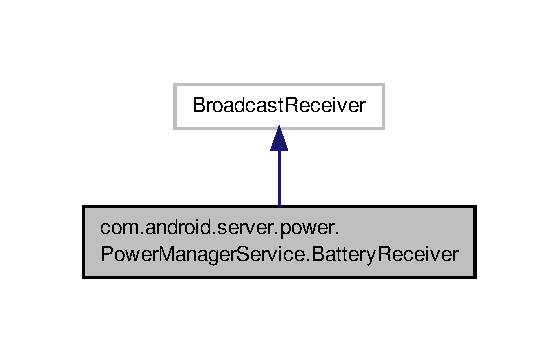
\includegraphics[width=268pt]{classcom_1_1android_1_1server_1_1power_1_1PowerManagerService_1_1BatteryReceiver__inherit__graph}
\end{center}
\end{figure}


Collaboration diagram for com.\-android.\-server.\-power.\-Power\-Manager\-Service.\-Battery\-Receiver\-:
\nopagebreak
\begin{figure}[H]
\begin{center}
\leavevmode
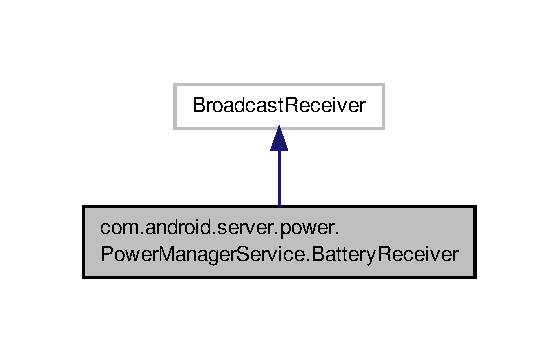
\includegraphics[width=268pt]{classcom_1_1android_1_1server_1_1power_1_1PowerManagerService_1_1BatteryReceiver__coll__graph}
\end{center}
\end{figure}
\subsection*{Public Member Functions}
\begin{DoxyCompactItemize}
\item 
void \hyperlink{classcom_1_1android_1_1server_1_1power_1_1PowerManagerService_1_1BatteryReceiver_a6de53659a9ad464737178de62a15fc42}{on\-Receive} (Context context, Intent intent)
\end{DoxyCompactItemize}


\subsection{Member Function Documentation}
\hypertarget{classcom_1_1android_1_1server_1_1power_1_1PowerManagerService_1_1BatteryReceiver_a6de53659a9ad464737178de62a15fc42}{\index{com\-::android\-::server\-::power\-::\-Power\-Manager\-Service\-::\-Battery\-Receiver@{com\-::android\-::server\-::power\-::\-Power\-Manager\-Service\-::\-Battery\-Receiver}!on\-Receive@{on\-Receive}}
\index{on\-Receive@{on\-Receive}!com::android::server::power::PowerManagerService::BatteryReceiver@{com\-::android\-::server\-::power\-::\-Power\-Manager\-Service\-::\-Battery\-Receiver}}
\subsubsection[{on\-Receive}]{\setlength{\rightskip}{0pt plus 5cm}void com.\-android.\-server.\-power.\-Power\-Manager\-Service.\-Battery\-Receiver.\-on\-Receive (
\begin{DoxyParamCaption}
\item[{Context}]{context, }
\item[{Intent}]{intent}
\end{DoxyParamCaption}
)\hspace{0.3cm}{\ttfamily [inline]}}}\label{classcom_1_1android_1_1server_1_1power_1_1PowerManagerService_1_1BatteryReceiver_a6de53659a9ad464737178de62a15fc42}


Here is the call graph for this function\-:
\nopagebreak
\begin{figure}[H]
\begin{center}
\leavevmode
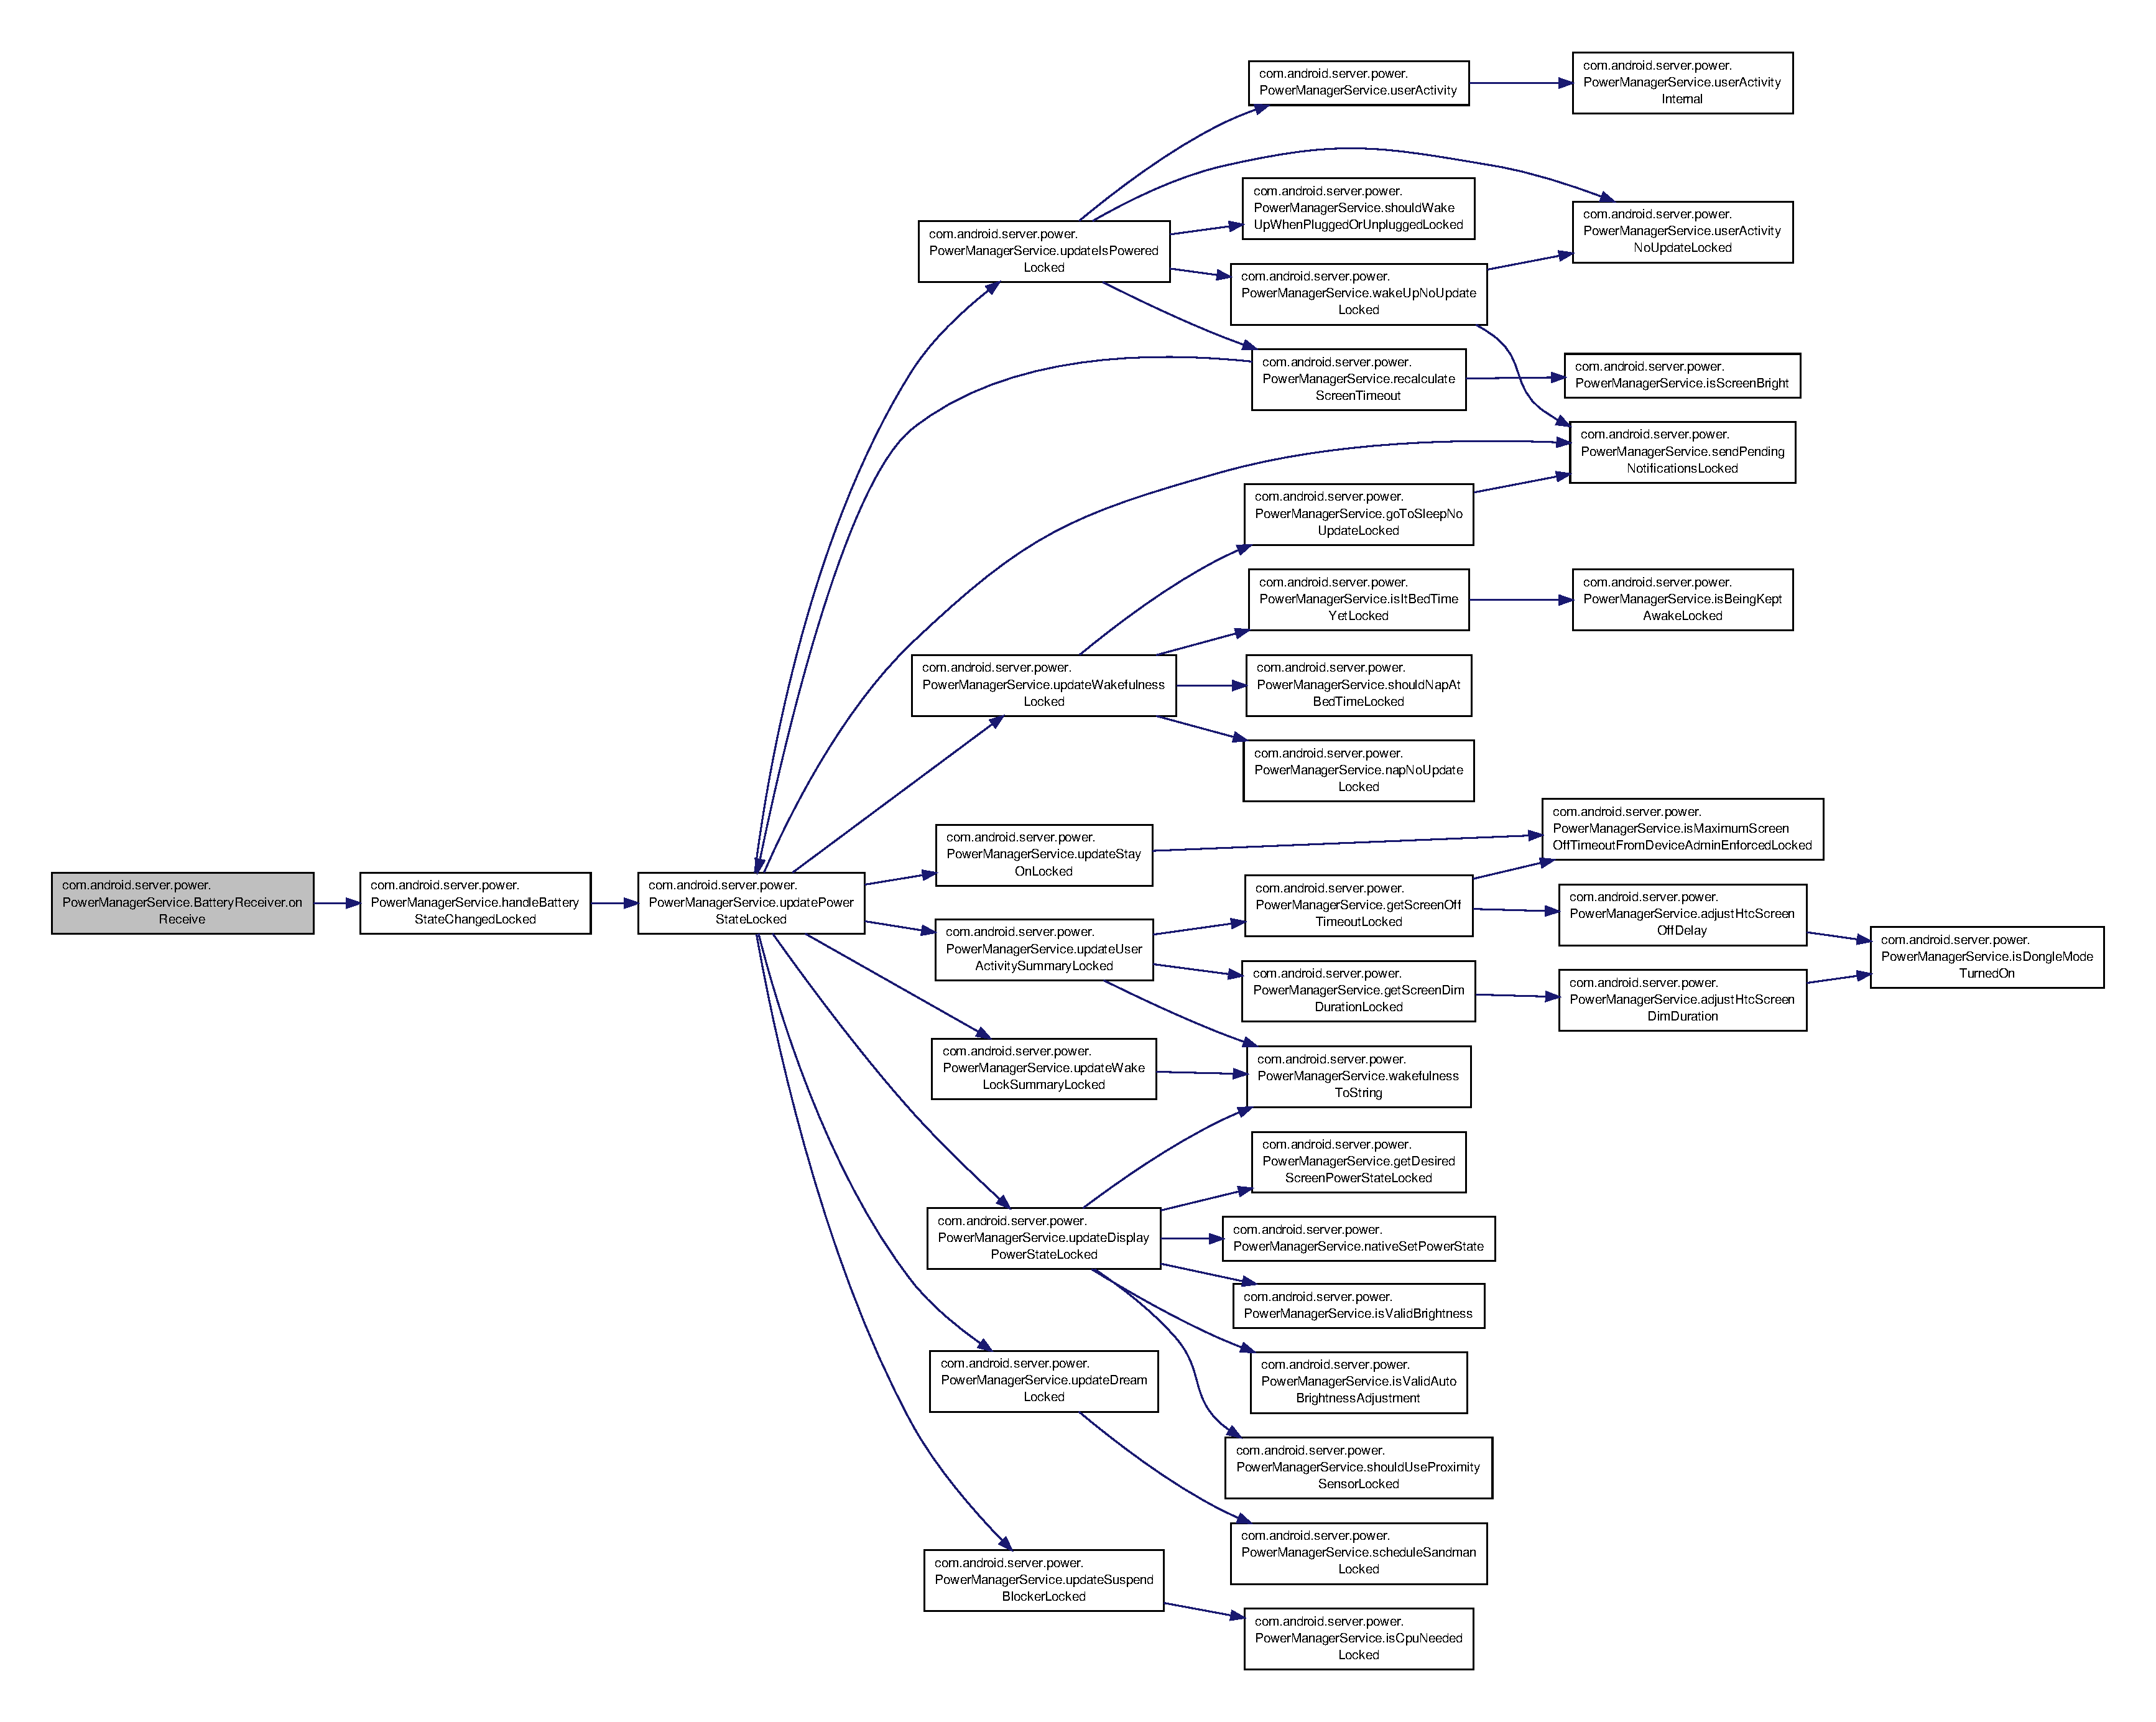
\includegraphics[width=350pt]{classcom_1_1android_1_1server_1_1power_1_1PowerManagerService_1_1BatteryReceiver_a6de53659a9ad464737178de62a15fc42_cgraph}
\end{center}
\end{figure}




The documentation for this class was generated from the following file\-:\begin{DoxyCompactItemize}
\item 
\hyperlink{PowerManagerService_8java}{Power\-Manager\-Service.\-java}\end{DoxyCompactItemize}

\hypertarget{classcom_1_1android_1_1server_1_1power_1_1PowerManagerService_1_1BootCompletedReceiver}{\section{com.\-android.\-server.\-power.\-Power\-Manager\-Service.\-Boot\-Completed\-Receiver Class Reference}
\label{classcom_1_1android_1_1server_1_1power_1_1PowerManagerService_1_1BootCompletedReceiver}\index{com.\-android.\-server.\-power.\-Power\-Manager\-Service.\-Boot\-Completed\-Receiver@{com.\-android.\-server.\-power.\-Power\-Manager\-Service.\-Boot\-Completed\-Receiver}}
}


Inheritance diagram for com.\-android.\-server.\-power.\-Power\-Manager\-Service.\-Boot\-Completed\-Receiver\-:
\nopagebreak
\begin{figure}[H]
\begin{center}
\leavevmode
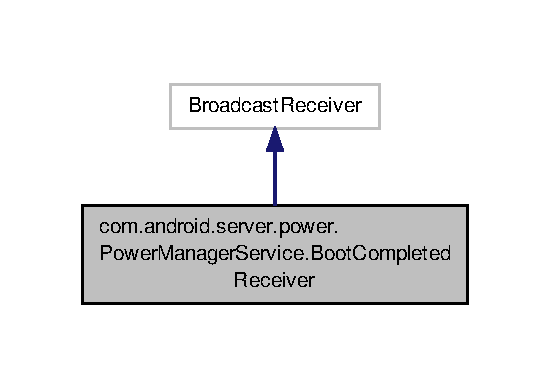
\includegraphics[width=264pt]{classcom_1_1android_1_1server_1_1power_1_1PowerManagerService_1_1BootCompletedReceiver__inherit__graph}
\end{center}
\end{figure}


Collaboration diagram for com.\-android.\-server.\-power.\-Power\-Manager\-Service.\-Boot\-Completed\-Receiver\-:
\nopagebreak
\begin{figure}[H]
\begin{center}
\leavevmode
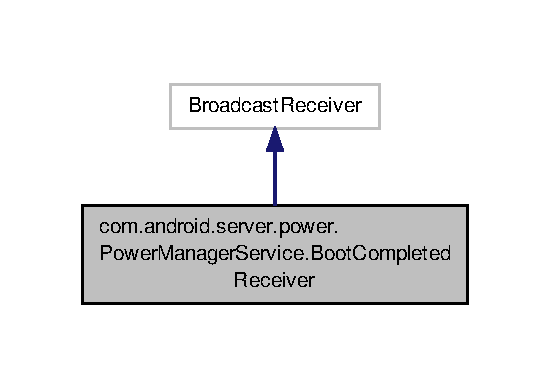
\includegraphics[width=264pt]{classcom_1_1android_1_1server_1_1power_1_1PowerManagerService_1_1BootCompletedReceiver__coll__graph}
\end{center}
\end{figure}
\subsection*{Public Member Functions}
\begin{DoxyCompactItemize}
\item 
void \hyperlink{classcom_1_1android_1_1server_1_1power_1_1PowerManagerService_1_1BootCompletedReceiver_a94ceb3bc4a7f0a01cffa720cb483f098}{on\-Receive} (Context context, Intent intent)
\end{DoxyCompactItemize}


\subsection{Member Function Documentation}
\hypertarget{classcom_1_1android_1_1server_1_1power_1_1PowerManagerService_1_1BootCompletedReceiver_a94ceb3bc4a7f0a01cffa720cb483f098}{\index{com\-::android\-::server\-::power\-::\-Power\-Manager\-Service\-::\-Boot\-Completed\-Receiver@{com\-::android\-::server\-::power\-::\-Power\-Manager\-Service\-::\-Boot\-Completed\-Receiver}!on\-Receive@{on\-Receive}}
\index{on\-Receive@{on\-Receive}!com::android::server::power::PowerManagerService::BootCompletedReceiver@{com\-::android\-::server\-::power\-::\-Power\-Manager\-Service\-::\-Boot\-Completed\-Receiver}}
\subsubsection[{on\-Receive}]{\setlength{\rightskip}{0pt plus 5cm}void com.\-android.\-server.\-power.\-Power\-Manager\-Service.\-Boot\-Completed\-Receiver.\-on\-Receive (
\begin{DoxyParamCaption}
\item[{Context}]{context, }
\item[{Intent}]{intent}
\end{DoxyParamCaption}
)\hspace{0.3cm}{\ttfamily [inline]}}}\label{classcom_1_1android_1_1server_1_1power_1_1PowerManagerService_1_1BootCompletedReceiver_a94ceb3bc4a7f0a01cffa720cb483f098}


Here is the call graph for this function\-:
\nopagebreak
\begin{figure}[H]
\begin{center}
\leavevmode
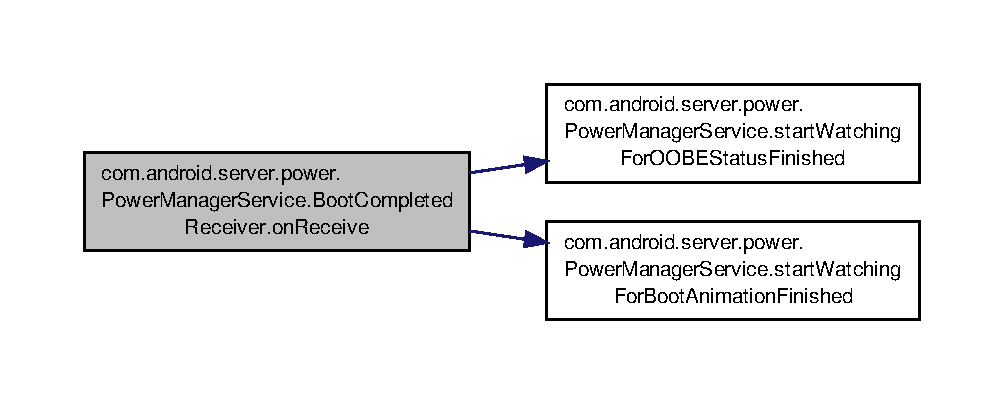
\includegraphics[width=350pt]{classcom_1_1android_1_1server_1_1power_1_1PowerManagerService_1_1BootCompletedReceiver_a94ceb3bc4a7f0a01cffa720cb483f098_cgraph}
\end{center}
\end{figure}




The documentation for this class was generated from the following file\-:\begin{DoxyCompactItemize}
\item 
\hyperlink{PowerManagerService_8java}{Power\-Manager\-Service.\-java}\end{DoxyCompactItemize}

\hypertarget{interfacecom_1_1android_1_1server_1_1power_1_1DisplayPowerController_1_1Callbacks}{\section{com.\-android.\-server.\-power.\-Display\-Power\-Controller.\-Callbacks Interface Reference}
\label{interfacecom_1_1android_1_1server_1_1power_1_1DisplayPowerController_1_1Callbacks}\index{com.\-android.\-server.\-power.\-Display\-Power\-Controller.\-Callbacks@{com.\-android.\-server.\-power.\-Display\-Power\-Controller.\-Callbacks}}
}
\subsection*{Public Member Functions}
\begin{DoxyCompactItemize}
\item 
void \hyperlink{interfacecom_1_1android_1_1server_1_1power_1_1DisplayPowerController_1_1Callbacks_a835253ee700d0bc38de6dd75f02fbb89}{on\-State\-Changed} ()
\item 
void \hyperlink{interfacecom_1_1android_1_1server_1_1power_1_1DisplayPowerController_1_1Callbacks_ac409b04585db7e8c3dba79a9e341608e}{on\-Proximity\-Positive} ()
\item 
void \hyperlink{interfacecom_1_1android_1_1server_1_1power_1_1DisplayPowerController_1_1Callbacks_aa99816ae70cdf6fdeea318054a18319a}{on\-Proximity\-Negative} ()
\item 
void \hyperlink{interfacecom_1_1android_1_1server_1_1power_1_1DisplayPowerController_1_1Callbacks_a9d3ddfd702875172756518fadf5c7563}{on\-Angle\-Detector\-Talking\-Detected} ()
\item 
void \hyperlink{interfacecom_1_1android_1_1server_1_1power_1_1DisplayPowerController_1_1Callbacks_a27ae924ac862c1eaa29c9a63b309eee6}{on\-Angle\-Detector\-Reading\-Detected} ()
\end{DoxyCompactItemize}


\subsection{Detailed Description}
Asynchronous callbacks from the power controller to the power manager service. 

\subsection{Member Function Documentation}
\hypertarget{interfacecom_1_1android_1_1server_1_1power_1_1DisplayPowerController_1_1Callbacks_a27ae924ac862c1eaa29c9a63b309eee6}{\index{com\-::android\-::server\-::power\-::\-Display\-Power\-Controller\-::\-Callbacks@{com\-::android\-::server\-::power\-::\-Display\-Power\-Controller\-::\-Callbacks}!on\-Angle\-Detector\-Reading\-Detected@{on\-Angle\-Detector\-Reading\-Detected}}
\index{on\-Angle\-Detector\-Reading\-Detected@{on\-Angle\-Detector\-Reading\-Detected}!com::android::server::power::DisplayPowerController::Callbacks@{com\-::android\-::server\-::power\-::\-Display\-Power\-Controller\-::\-Callbacks}}
\subsubsection[{on\-Angle\-Detector\-Reading\-Detected}]{\setlength{\rightskip}{0pt plus 5cm}void com.\-android.\-server.\-power.\-Display\-Power\-Controller.\-Callbacks.\-on\-Angle\-Detector\-Reading\-Detected (
\begin{DoxyParamCaption}
{}
\end{DoxyParamCaption}
)}}\label{interfacecom_1_1android_1_1server_1_1power_1_1DisplayPowerController_1_1Callbacks_a27ae924ac862c1eaa29c9a63b309eee6}
\hypertarget{interfacecom_1_1android_1_1server_1_1power_1_1DisplayPowerController_1_1Callbacks_a9d3ddfd702875172756518fadf5c7563}{\index{com\-::android\-::server\-::power\-::\-Display\-Power\-Controller\-::\-Callbacks@{com\-::android\-::server\-::power\-::\-Display\-Power\-Controller\-::\-Callbacks}!on\-Angle\-Detector\-Talking\-Detected@{on\-Angle\-Detector\-Talking\-Detected}}
\index{on\-Angle\-Detector\-Talking\-Detected@{on\-Angle\-Detector\-Talking\-Detected}!com::android::server::power::DisplayPowerController::Callbacks@{com\-::android\-::server\-::power\-::\-Display\-Power\-Controller\-::\-Callbacks}}
\subsubsection[{on\-Angle\-Detector\-Talking\-Detected}]{\setlength{\rightskip}{0pt plus 5cm}void com.\-android.\-server.\-power.\-Display\-Power\-Controller.\-Callbacks.\-on\-Angle\-Detector\-Talking\-Detected (
\begin{DoxyParamCaption}
{}
\end{DoxyParamCaption}
)}}\label{interfacecom_1_1android_1_1server_1_1power_1_1DisplayPowerController_1_1Callbacks_a9d3ddfd702875172756518fadf5c7563}
\hypertarget{interfacecom_1_1android_1_1server_1_1power_1_1DisplayPowerController_1_1Callbacks_aa99816ae70cdf6fdeea318054a18319a}{\index{com\-::android\-::server\-::power\-::\-Display\-Power\-Controller\-::\-Callbacks@{com\-::android\-::server\-::power\-::\-Display\-Power\-Controller\-::\-Callbacks}!on\-Proximity\-Negative@{on\-Proximity\-Negative}}
\index{on\-Proximity\-Negative@{on\-Proximity\-Negative}!com::android::server::power::DisplayPowerController::Callbacks@{com\-::android\-::server\-::power\-::\-Display\-Power\-Controller\-::\-Callbacks}}
\subsubsection[{on\-Proximity\-Negative}]{\setlength{\rightskip}{0pt plus 5cm}void com.\-android.\-server.\-power.\-Display\-Power\-Controller.\-Callbacks.\-on\-Proximity\-Negative (
\begin{DoxyParamCaption}
{}
\end{DoxyParamCaption}
)}}\label{interfacecom_1_1android_1_1server_1_1power_1_1DisplayPowerController_1_1Callbacks_aa99816ae70cdf6fdeea318054a18319a}
\hypertarget{interfacecom_1_1android_1_1server_1_1power_1_1DisplayPowerController_1_1Callbacks_ac409b04585db7e8c3dba79a9e341608e}{\index{com\-::android\-::server\-::power\-::\-Display\-Power\-Controller\-::\-Callbacks@{com\-::android\-::server\-::power\-::\-Display\-Power\-Controller\-::\-Callbacks}!on\-Proximity\-Positive@{on\-Proximity\-Positive}}
\index{on\-Proximity\-Positive@{on\-Proximity\-Positive}!com::android::server::power::DisplayPowerController::Callbacks@{com\-::android\-::server\-::power\-::\-Display\-Power\-Controller\-::\-Callbacks}}
\subsubsection[{on\-Proximity\-Positive}]{\setlength{\rightskip}{0pt plus 5cm}void com.\-android.\-server.\-power.\-Display\-Power\-Controller.\-Callbacks.\-on\-Proximity\-Positive (
\begin{DoxyParamCaption}
{}
\end{DoxyParamCaption}
)}}\label{interfacecom_1_1android_1_1server_1_1power_1_1DisplayPowerController_1_1Callbacks_ac409b04585db7e8c3dba79a9e341608e}
\hypertarget{interfacecom_1_1android_1_1server_1_1power_1_1DisplayPowerController_1_1Callbacks_a835253ee700d0bc38de6dd75f02fbb89}{\index{com\-::android\-::server\-::power\-::\-Display\-Power\-Controller\-::\-Callbacks@{com\-::android\-::server\-::power\-::\-Display\-Power\-Controller\-::\-Callbacks}!on\-State\-Changed@{on\-State\-Changed}}
\index{on\-State\-Changed@{on\-State\-Changed}!com::android::server::power::DisplayPowerController::Callbacks@{com\-::android\-::server\-::power\-::\-Display\-Power\-Controller\-::\-Callbacks}}
\subsubsection[{on\-State\-Changed}]{\setlength{\rightskip}{0pt plus 5cm}void com.\-android.\-server.\-power.\-Display\-Power\-Controller.\-Callbacks.\-on\-State\-Changed (
\begin{DoxyParamCaption}
{}
\end{DoxyParamCaption}
)}}\label{interfacecom_1_1android_1_1server_1_1power_1_1DisplayPowerController_1_1Callbacks_a835253ee700d0bc38de6dd75f02fbb89}


The documentation for this interface was generated from the following file\-:\begin{DoxyCompactItemize}
\item 
\hyperlink{DisplayPowerController_8java}{Display\-Power\-Controller.\-java}\end{DoxyCompactItemize}

\hypertarget{classcom_1_1android_1_1server_1_1power_1_1ShutdownThread_1_1CloseDialogReceiver}{\section{com.\-android.\-server.\-power.\-Shutdown\-Thread.\-Close\-Dialog\-Receiver Class Reference}
\label{classcom_1_1android_1_1server_1_1power_1_1ShutdownThread_1_1CloseDialogReceiver}\index{com.\-android.\-server.\-power.\-Shutdown\-Thread.\-Close\-Dialog\-Receiver@{com.\-android.\-server.\-power.\-Shutdown\-Thread.\-Close\-Dialog\-Receiver}}
}


Inheritance diagram for com.\-android.\-server.\-power.\-Shutdown\-Thread.\-Close\-Dialog\-Receiver\-:
\nopagebreak
\begin{figure}[H]
\begin{center}
\leavevmode
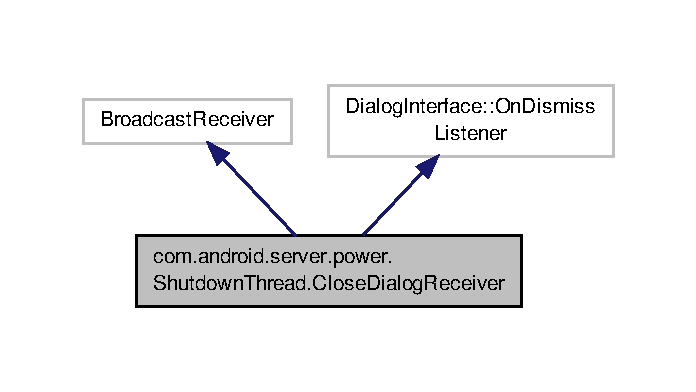
\includegraphics[width=334pt]{classcom_1_1android_1_1server_1_1power_1_1ShutdownThread_1_1CloseDialogReceiver__inherit__graph}
\end{center}
\end{figure}


Collaboration diagram for com.\-android.\-server.\-power.\-Shutdown\-Thread.\-Close\-Dialog\-Receiver\-:
\nopagebreak
\begin{figure}[H]
\begin{center}
\leavevmode
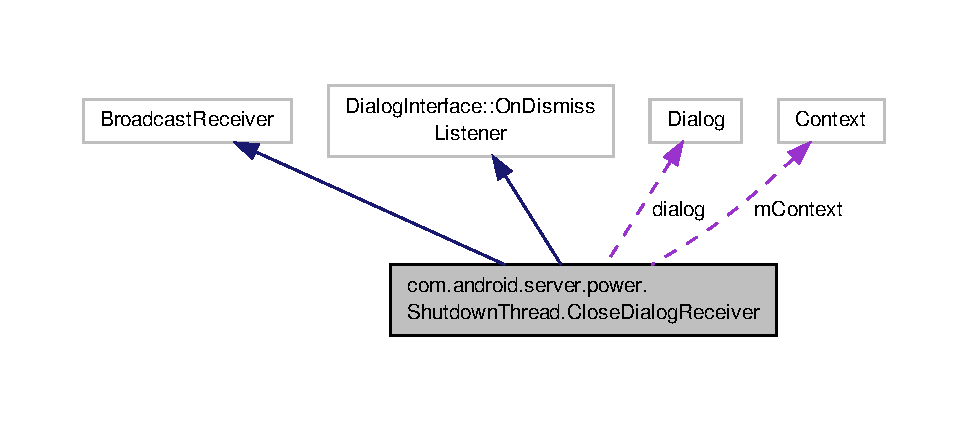
\includegraphics[width=350pt]{classcom_1_1android_1_1server_1_1power_1_1ShutdownThread_1_1CloseDialogReceiver__coll__graph}
\end{center}
\end{figure}
\subsection*{Public Member Functions}
\begin{DoxyCompactItemize}
\item 
void \hyperlink{classcom_1_1android_1_1server_1_1power_1_1ShutdownThread_1_1CloseDialogReceiver_a6f11c6d2c5343843e5b1194abd48623e}{on\-Receive} (Context context, Intent intent)
\item 
void \hyperlink{classcom_1_1android_1_1server_1_1power_1_1ShutdownThread_1_1CloseDialogReceiver_ae17a10bd92e80ad0961167a1af3ddadb}{on\-Dismiss} (Dialog\-Interface unused)
\end{DoxyCompactItemize}
\subsection*{Public Attributes}
\begin{DoxyCompactItemize}
\item 
Dialog \hyperlink{classcom_1_1android_1_1server_1_1power_1_1ShutdownThread_1_1CloseDialogReceiver_a93b406c3e8b9976aa981ee369846f775}{dialog}
\end{DoxyCompactItemize}
\subsection*{Private Attributes}
\begin{DoxyCompactItemize}
\item 
Context \hyperlink{classcom_1_1android_1_1server_1_1power_1_1ShutdownThread_1_1CloseDialogReceiver_a7f5161219feb6ce136795e9451047daf}{m\-Context}
\end{DoxyCompactItemize}


\subsection{Member Function Documentation}
\hypertarget{classcom_1_1android_1_1server_1_1power_1_1ShutdownThread_1_1CloseDialogReceiver_ae17a10bd92e80ad0961167a1af3ddadb}{\index{com\-::android\-::server\-::power\-::\-Shutdown\-Thread\-::\-Close\-Dialog\-Receiver@{com\-::android\-::server\-::power\-::\-Shutdown\-Thread\-::\-Close\-Dialog\-Receiver}!on\-Dismiss@{on\-Dismiss}}
\index{on\-Dismiss@{on\-Dismiss}!com::android::server::power::ShutdownThread::CloseDialogReceiver@{com\-::android\-::server\-::power\-::\-Shutdown\-Thread\-::\-Close\-Dialog\-Receiver}}
\subsubsection[{on\-Dismiss}]{\setlength{\rightskip}{0pt plus 5cm}void com.\-android.\-server.\-power.\-Shutdown\-Thread.\-Close\-Dialog\-Receiver.\-on\-Dismiss (
\begin{DoxyParamCaption}
\item[{Dialog\-Interface}]{unused}
\end{DoxyParamCaption}
)\hspace{0.3cm}{\ttfamily [inline]}}}\label{classcom_1_1android_1_1server_1_1power_1_1ShutdownThread_1_1CloseDialogReceiver_ae17a10bd92e80ad0961167a1af3ddadb}
\hypertarget{classcom_1_1android_1_1server_1_1power_1_1ShutdownThread_1_1CloseDialogReceiver_a6f11c6d2c5343843e5b1194abd48623e}{\index{com\-::android\-::server\-::power\-::\-Shutdown\-Thread\-::\-Close\-Dialog\-Receiver@{com\-::android\-::server\-::power\-::\-Shutdown\-Thread\-::\-Close\-Dialog\-Receiver}!on\-Receive@{on\-Receive}}
\index{on\-Receive@{on\-Receive}!com::android::server::power::ShutdownThread::CloseDialogReceiver@{com\-::android\-::server\-::power\-::\-Shutdown\-Thread\-::\-Close\-Dialog\-Receiver}}
\subsubsection[{on\-Receive}]{\setlength{\rightskip}{0pt plus 5cm}void com.\-android.\-server.\-power.\-Shutdown\-Thread.\-Close\-Dialog\-Receiver.\-on\-Receive (
\begin{DoxyParamCaption}
\item[{Context}]{context, }
\item[{Intent}]{intent}
\end{DoxyParamCaption}
)\hspace{0.3cm}{\ttfamily [inline]}}}\label{classcom_1_1android_1_1server_1_1power_1_1ShutdownThread_1_1CloseDialogReceiver_a6f11c6d2c5343843e5b1194abd48623e}


\subsection{Member Data Documentation}
\hypertarget{classcom_1_1android_1_1server_1_1power_1_1ShutdownThread_1_1CloseDialogReceiver_a93b406c3e8b9976aa981ee369846f775}{\index{com\-::android\-::server\-::power\-::\-Shutdown\-Thread\-::\-Close\-Dialog\-Receiver@{com\-::android\-::server\-::power\-::\-Shutdown\-Thread\-::\-Close\-Dialog\-Receiver}!dialog@{dialog}}
\index{dialog@{dialog}!com::android::server::power::ShutdownThread::CloseDialogReceiver@{com\-::android\-::server\-::power\-::\-Shutdown\-Thread\-::\-Close\-Dialog\-Receiver}}
\subsubsection[{dialog}]{\setlength{\rightskip}{0pt plus 5cm}Dialog com.\-android.\-server.\-power.\-Shutdown\-Thread.\-Close\-Dialog\-Receiver.\-dialog}}\label{classcom_1_1android_1_1server_1_1power_1_1ShutdownThread_1_1CloseDialogReceiver_a93b406c3e8b9976aa981ee369846f775}
\hypertarget{classcom_1_1android_1_1server_1_1power_1_1ShutdownThread_1_1CloseDialogReceiver_a7f5161219feb6ce136795e9451047daf}{\index{com\-::android\-::server\-::power\-::\-Shutdown\-Thread\-::\-Close\-Dialog\-Receiver@{com\-::android\-::server\-::power\-::\-Shutdown\-Thread\-::\-Close\-Dialog\-Receiver}!m\-Context@{m\-Context}}
\index{m\-Context@{m\-Context}!com::android::server::power::ShutdownThread::CloseDialogReceiver@{com\-::android\-::server\-::power\-::\-Shutdown\-Thread\-::\-Close\-Dialog\-Receiver}}
\subsubsection[{m\-Context}]{\setlength{\rightskip}{0pt plus 5cm}Context com.\-android.\-server.\-power.\-Shutdown\-Thread.\-Close\-Dialog\-Receiver.\-m\-Context\hspace{0.3cm}{\ttfamily [private]}}}\label{classcom_1_1android_1_1server_1_1power_1_1ShutdownThread_1_1CloseDialogReceiver_a7f5161219feb6ce136795e9451047daf}


The documentation for this class was generated from the following file\-:\begin{DoxyCompactItemize}
\item 
\hyperlink{ShutdownThread_8java}{Shutdown\-Thread.\-java}\end{DoxyCompactItemize}

\hypertarget{classcom_1_1android_1_1server_1_1power_1_1PowerManagerService_1_1DisplayBlankerImpl}{\section{com.\-android.\-server.\-power.\-Power\-Manager\-Service.\-Display\-Blanker\-Impl Class Reference}
\label{classcom_1_1android_1_1server_1_1power_1_1PowerManagerService_1_1DisplayBlankerImpl}\index{com.\-android.\-server.\-power.\-Power\-Manager\-Service.\-Display\-Blanker\-Impl@{com.\-android.\-server.\-power.\-Power\-Manager\-Service.\-Display\-Blanker\-Impl}}
}


Inheritance diagram for com.\-android.\-server.\-power.\-Power\-Manager\-Service.\-Display\-Blanker\-Impl\-:
\nopagebreak
\begin{figure}[H]
\begin{center}
\leavevmode
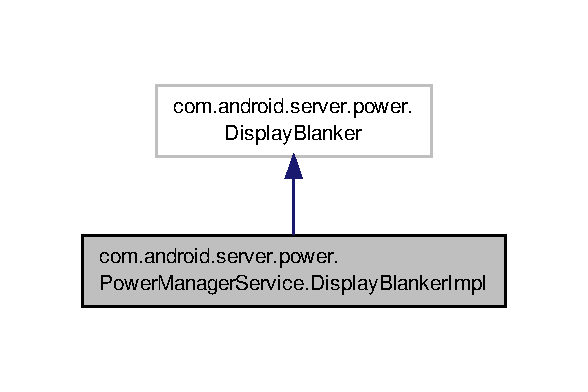
\includegraphics[width=282pt]{classcom_1_1android_1_1server_1_1power_1_1PowerManagerService_1_1DisplayBlankerImpl__inherit__graph}
\end{center}
\end{figure}


Collaboration diagram for com.\-android.\-server.\-power.\-Power\-Manager\-Service.\-Display\-Blanker\-Impl\-:
\nopagebreak
\begin{figure}[H]
\begin{center}
\leavevmode
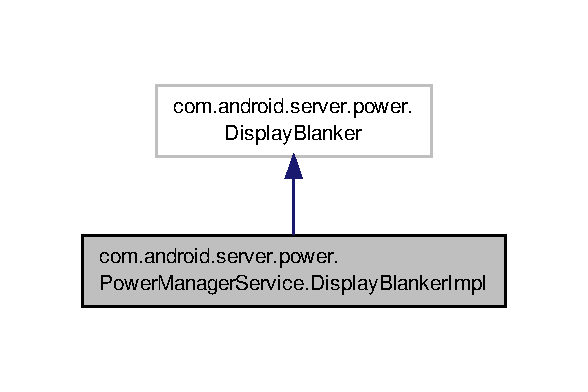
\includegraphics[width=282pt]{classcom_1_1android_1_1server_1_1power_1_1PowerManagerService_1_1DisplayBlankerImpl__coll__graph}
\end{center}
\end{figure}
\subsection*{Public Member Functions}
\begin{DoxyCompactItemize}
\item 
void \hyperlink{classcom_1_1android_1_1server_1_1power_1_1PowerManagerService_1_1DisplayBlankerImpl_a44d0289807a476d574b0c5545520c937}{blank\-All\-Displays} ()
\item 
void \hyperlink{classcom_1_1android_1_1server_1_1power_1_1PowerManagerService_1_1DisplayBlankerImpl_a7bf7b567ffe18d6263bba13baa1f8673}{unblank\-All\-Displays} ()
\item 
String \hyperlink{classcom_1_1android_1_1server_1_1power_1_1PowerManagerService_1_1DisplayBlankerImpl_a73bfd3b63c1fb9424a7e3a7d08c6bbf4}{to\-String} ()
\end{DoxyCompactItemize}
\subsection*{Private Member Functions}
\begin{DoxyCompactItemize}
\item 
void \hyperlink{classcom_1_1android_1_1server_1_1power_1_1PowerManagerService_1_1DisplayBlankerImpl_a2b01016d7172201aae2e8f417327c84d}{screen\-State\-Notifier} (boolean on)
\end{DoxyCompactItemize}
\subsection*{Private Attributes}
\begin{DoxyCompactItemize}
\item 
boolean \hyperlink{classcom_1_1android_1_1server_1_1power_1_1PowerManagerService_1_1DisplayBlankerImpl_a2588920f9e1fca260ee7a4e4738c5bed}{m\-Blanked}
\end{DoxyCompactItemize}


\subsection{Member Function Documentation}
\hypertarget{classcom_1_1android_1_1server_1_1power_1_1PowerManagerService_1_1DisplayBlankerImpl_a44d0289807a476d574b0c5545520c937}{\index{com\-::android\-::server\-::power\-::\-Power\-Manager\-Service\-::\-Display\-Blanker\-Impl@{com\-::android\-::server\-::power\-::\-Power\-Manager\-Service\-::\-Display\-Blanker\-Impl}!blank\-All\-Displays@{blank\-All\-Displays}}
\index{blank\-All\-Displays@{blank\-All\-Displays}!com::android::server::power::PowerManagerService::DisplayBlankerImpl@{com\-::android\-::server\-::power\-::\-Power\-Manager\-Service\-::\-Display\-Blanker\-Impl}}
\subsubsection[{blank\-All\-Displays}]{\setlength{\rightskip}{0pt plus 5cm}void com.\-android.\-server.\-power.\-Power\-Manager\-Service.\-Display\-Blanker\-Impl.\-blank\-All\-Displays (
\begin{DoxyParamCaption}
{}
\end{DoxyParamCaption}
)\hspace{0.3cm}{\ttfamily [inline]}}}\label{classcom_1_1android_1_1server_1_1power_1_1PowerManagerService_1_1DisplayBlankerImpl_a44d0289807a476d574b0c5545520c937}


Here is the call graph for this function\-:
\nopagebreak
\begin{figure}[H]
\begin{center}
\leavevmode
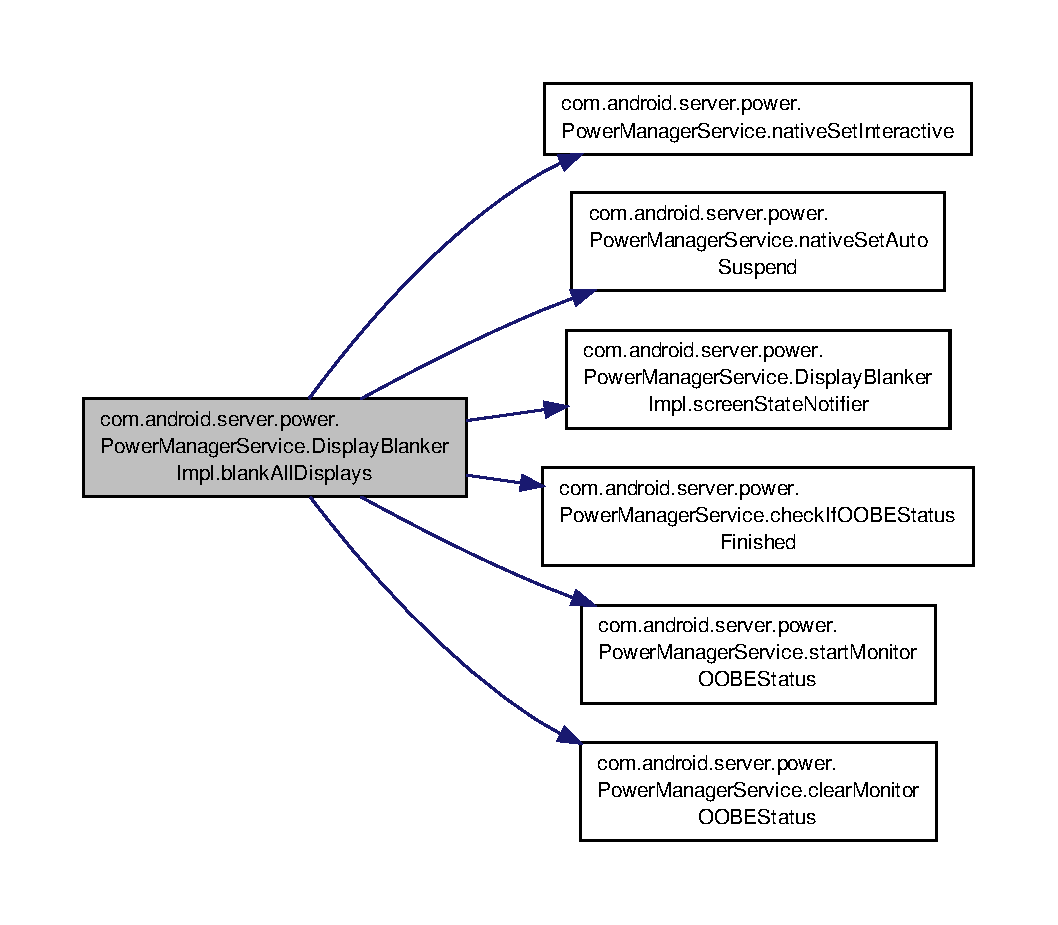
\includegraphics[width=350pt]{classcom_1_1android_1_1server_1_1power_1_1PowerManagerService_1_1DisplayBlankerImpl_a44d0289807a476d574b0c5545520c937_cgraph}
\end{center}
\end{figure}


\hypertarget{classcom_1_1android_1_1server_1_1power_1_1PowerManagerService_1_1DisplayBlankerImpl_a2b01016d7172201aae2e8f417327c84d}{\index{com\-::android\-::server\-::power\-::\-Power\-Manager\-Service\-::\-Display\-Blanker\-Impl@{com\-::android\-::server\-::power\-::\-Power\-Manager\-Service\-::\-Display\-Blanker\-Impl}!screen\-State\-Notifier@{screen\-State\-Notifier}}
\index{screen\-State\-Notifier@{screen\-State\-Notifier}!com::android::server::power::PowerManagerService::DisplayBlankerImpl@{com\-::android\-::server\-::power\-::\-Power\-Manager\-Service\-::\-Display\-Blanker\-Impl}}
\subsubsection[{screen\-State\-Notifier}]{\setlength{\rightskip}{0pt plus 5cm}void com.\-android.\-server.\-power.\-Power\-Manager\-Service.\-Display\-Blanker\-Impl.\-screen\-State\-Notifier (
\begin{DoxyParamCaption}
\item[{boolean}]{on}
\end{DoxyParamCaption}
)\hspace{0.3cm}{\ttfamily [inline]}, {\ttfamily [private]}}}\label{classcom_1_1android_1_1server_1_1power_1_1PowerManagerService_1_1DisplayBlankerImpl_a2b01016d7172201aae2e8f417327c84d}
\hypertarget{classcom_1_1android_1_1server_1_1power_1_1PowerManagerService_1_1DisplayBlankerImpl_a73bfd3b63c1fb9424a7e3a7d08c6bbf4}{\index{com\-::android\-::server\-::power\-::\-Power\-Manager\-Service\-::\-Display\-Blanker\-Impl@{com\-::android\-::server\-::power\-::\-Power\-Manager\-Service\-::\-Display\-Blanker\-Impl}!to\-String@{to\-String}}
\index{to\-String@{to\-String}!com::android::server::power::PowerManagerService::DisplayBlankerImpl@{com\-::android\-::server\-::power\-::\-Power\-Manager\-Service\-::\-Display\-Blanker\-Impl}}
\subsubsection[{to\-String}]{\setlength{\rightskip}{0pt plus 5cm}String com.\-android.\-server.\-power.\-Power\-Manager\-Service.\-Display\-Blanker\-Impl.\-to\-String (
\begin{DoxyParamCaption}
{}
\end{DoxyParamCaption}
)\hspace{0.3cm}{\ttfamily [inline]}}}\label{classcom_1_1android_1_1server_1_1power_1_1PowerManagerService_1_1DisplayBlankerImpl_a73bfd3b63c1fb9424a7e3a7d08c6bbf4}
\hypertarget{classcom_1_1android_1_1server_1_1power_1_1PowerManagerService_1_1DisplayBlankerImpl_a7bf7b567ffe18d6263bba13baa1f8673}{\index{com\-::android\-::server\-::power\-::\-Power\-Manager\-Service\-::\-Display\-Blanker\-Impl@{com\-::android\-::server\-::power\-::\-Power\-Manager\-Service\-::\-Display\-Blanker\-Impl}!unblank\-All\-Displays@{unblank\-All\-Displays}}
\index{unblank\-All\-Displays@{unblank\-All\-Displays}!com::android::server::power::PowerManagerService::DisplayBlankerImpl@{com\-::android\-::server\-::power\-::\-Power\-Manager\-Service\-::\-Display\-Blanker\-Impl}}
\subsubsection[{unblank\-All\-Displays}]{\setlength{\rightskip}{0pt plus 5cm}void com.\-android.\-server.\-power.\-Power\-Manager\-Service.\-Display\-Blanker\-Impl.\-unblank\-All\-Displays (
\begin{DoxyParamCaption}
{}
\end{DoxyParamCaption}
)\hspace{0.3cm}{\ttfamily [inline]}}}\label{classcom_1_1android_1_1server_1_1power_1_1PowerManagerService_1_1DisplayBlankerImpl_a7bf7b567ffe18d6263bba13baa1f8673}


Here is the call graph for this function\-:
\nopagebreak
\begin{figure}[H]
\begin{center}
\leavevmode
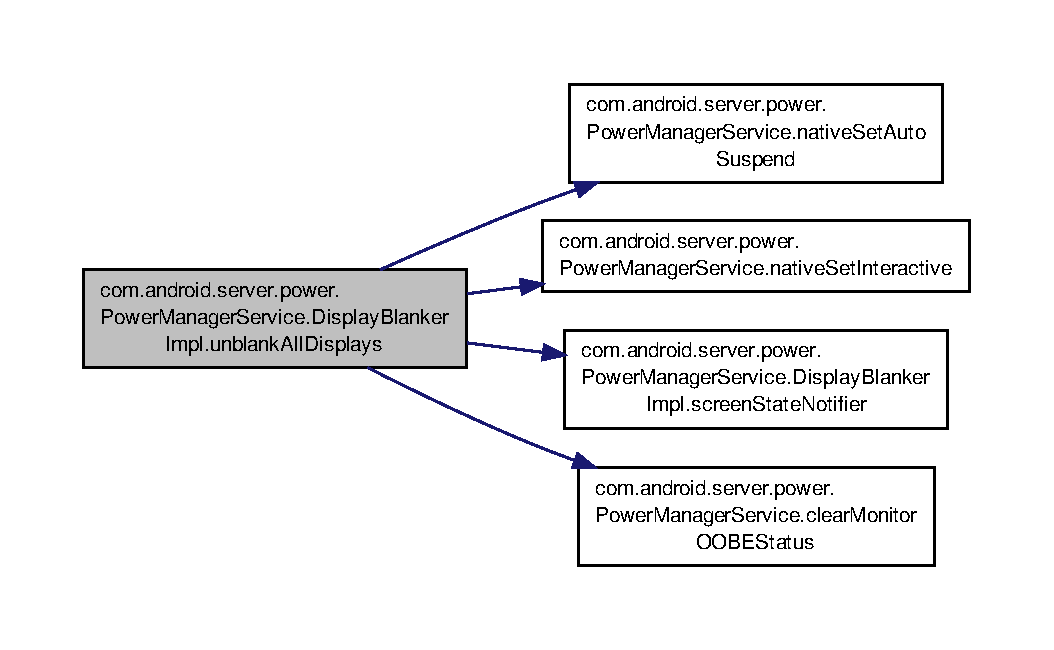
\includegraphics[width=350pt]{classcom_1_1android_1_1server_1_1power_1_1PowerManagerService_1_1DisplayBlankerImpl_a7bf7b567ffe18d6263bba13baa1f8673_cgraph}
\end{center}
\end{figure}




\subsection{Member Data Documentation}
\hypertarget{classcom_1_1android_1_1server_1_1power_1_1PowerManagerService_1_1DisplayBlankerImpl_a2588920f9e1fca260ee7a4e4738c5bed}{\index{com\-::android\-::server\-::power\-::\-Power\-Manager\-Service\-::\-Display\-Blanker\-Impl@{com\-::android\-::server\-::power\-::\-Power\-Manager\-Service\-::\-Display\-Blanker\-Impl}!m\-Blanked@{m\-Blanked}}
\index{m\-Blanked@{m\-Blanked}!com::android::server::power::PowerManagerService::DisplayBlankerImpl@{com\-::android\-::server\-::power\-::\-Power\-Manager\-Service\-::\-Display\-Blanker\-Impl}}
\subsubsection[{m\-Blanked}]{\setlength{\rightskip}{0pt plus 5cm}boolean com.\-android.\-server.\-power.\-Power\-Manager\-Service.\-Display\-Blanker\-Impl.\-m\-Blanked\hspace{0.3cm}{\ttfamily [private]}}}\label{classcom_1_1android_1_1server_1_1power_1_1PowerManagerService_1_1DisplayBlankerImpl_a2588920f9e1fca260ee7a4e4738c5bed}


The documentation for this class was generated from the following file\-:\begin{DoxyCompactItemize}
\item 
\hyperlink{PowerManagerService_8java}{Power\-Manager\-Service.\-java}\end{DoxyCompactItemize}

\hypertarget{classcom_1_1android_1_1server_1_1power_1_1DisplayPowerController_1_1DisplayControllerHandler}{\section{com.\-android.\-server.\-power.\-Display\-Power\-Controller.\-Display\-Controller\-Handler Class Reference}
\label{classcom_1_1android_1_1server_1_1power_1_1DisplayPowerController_1_1DisplayControllerHandler}\index{com.\-android.\-server.\-power.\-Display\-Power\-Controller.\-Display\-Controller\-Handler@{com.\-android.\-server.\-power.\-Display\-Power\-Controller.\-Display\-Controller\-Handler}}
}


Inheritance diagram for com.\-android.\-server.\-power.\-Display\-Power\-Controller.\-Display\-Controller\-Handler\-:
\nopagebreak
\begin{figure}[H]
\begin{center}
\leavevmode
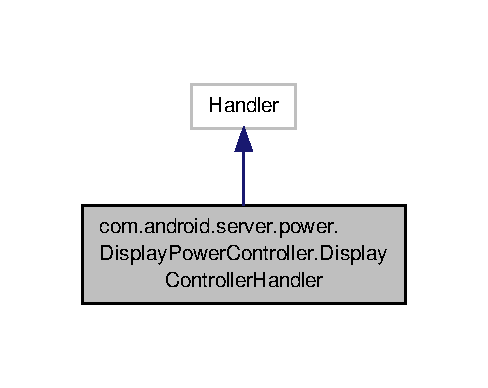
\includegraphics[width=234pt]{classcom_1_1android_1_1server_1_1power_1_1DisplayPowerController_1_1DisplayControllerHandler__inherit__graph}
\end{center}
\end{figure}


Collaboration diagram for com.\-android.\-server.\-power.\-Display\-Power\-Controller.\-Display\-Controller\-Handler\-:
\nopagebreak
\begin{figure}[H]
\begin{center}
\leavevmode
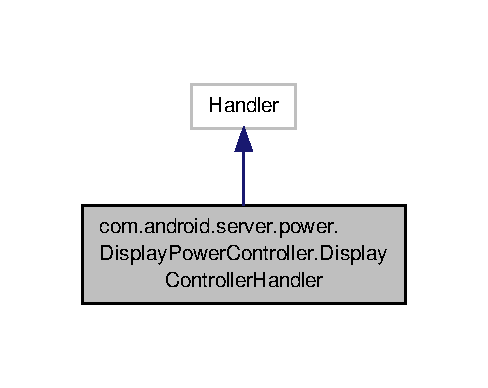
\includegraphics[width=234pt]{classcom_1_1android_1_1server_1_1power_1_1DisplayPowerController_1_1DisplayControllerHandler__coll__graph}
\end{center}
\end{figure}
\subsection*{Public Member Functions}
\begin{DoxyCompactItemize}
\item 
\hyperlink{classcom_1_1android_1_1server_1_1power_1_1DisplayPowerController_1_1DisplayControllerHandler_a8474bdda5d5b42c48896d58cee4fceac}{Display\-Controller\-Handler} (Looper looper)
\item 
void \hyperlink{classcom_1_1android_1_1server_1_1power_1_1DisplayPowerController_1_1DisplayControllerHandler_af41eba45590974d63993f9d85409d706}{handle\-Message} (Message msg)
\end{DoxyCompactItemize}


\subsection{Constructor \& Destructor Documentation}
\hypertarget{classcom_1_1android_1_1server_1_1power_1_1DisplayPowerController_1_1DisplayControllerHandler_a8474bdda5d5b42c48896d58cee4fceac}{\index{com\-::android\-::server\-::power\-::\-Display\-Power\-Controller\-::\-Display\-Controller\-Handler@{com\-::android\-::server\-::power\-::\-Display\-Power\-Controller\-::\-Display\-Controller\-Handler}!Display\-Controller\-Handler@{Display\-Controller\-Handler}}
\index{Display\-Controller\-Handler@{Display\-Controller\-Handler}!com::android::server::power::DisplayPowerController::DisplayControllerHandler@{com\-::android\-::server\-::power\-::\-Display\-Power\-Controller\-::\-Display\-Controller\-Handler}}
\subsubsection[{Display\-Controller\-Handler}]{\setlength{\rightskip}{0pt plus 5cm}com.\-android.\-server.\-power.\-Display\-Power\-Controller.\-Display\-Controller\-Handler.\-Display\-Controller\-Handler (
\begin{DoxyParamCaption}
\item[{Looper}]{looper}
\end{DoxyParamCaption}
)\hspace{0.3cm}{\ttfamily [inline]}}}\label{classcom_1_1android_1_1server_1_1power_1_1DisplayPowerController_1_1DisplayControllerHandler_a8474bdda5d5b42c48896d58cee4fceac}


\subsection{Member Function Documentation}
\hypertarget{classcom_1_1android_1_1server_1_1power_1_1DisplayPowerController_1_1DisplayControllerHandler_af41eba45590974d63993f9d85409d706}{\index{com\-::android\-::server\-::power\-::\-Display\-Power\-Controller\-::\-Display\-Controller\-Handler@{com\-::android\-::server\-::power\-::\-Display\-Power\-Controller\-::\-Display\-Controller\-Handler}!handle\-Message@{handle\-Message}}
\index{handle\-Message@{handle\-Message}!com::android::server::power::DisplayPowerController::DisplayControllerHandler@{com\-::android\-::server\-::power\-::\-Display\-Power\-Controller\-::\-Display\-Controller\-Handler}}
\subsubsection[{handle\-Message}]{\setlength{\rightskip}{0pt plus 5cm}void com.\-android.\-server.\-power.\-Display\-Power\-Controller.\-Display\-Controller\-Handler.\-handle\-Message (
\begin{DoxyParamCaption}
\item[{Message}]{msg}
\end{DoxyParamCaption}
)\hspace{0.3cm}{\ttfamily [inline]}}}\label{classcom_1_1android_1_1server_1_1power_1_1DisplayPowerController_1_1DisplayControllerHandler_af41eba45590974d63993f9d85409d706}


The documentation for this class was generated from the following file\-:\begin{DoxyCompactItemize}
\item 
\hyperlink{DisplayPowerController_8java}{Display\-Power\-Controller.\-java}\end{DoxyCompactItemize}

\hypertarget{classcom_1_1android_1_1server_1_1power_1_1PowerManagerService_1_1DockReceiver}{\section{com.\-android.\-server.\-power.\-Power\-Manager\-Service.\-Dock\-Receiver Class Reference}
\label{classcom_1_1android_1_1server_1_1power_1_1PowerManagerService_1_1DockReceiver}\index{com.\-android.\-server.\-power.\-Power\-Manager\-Service.\-Dock\-Receiver@{com.\-android.\-server.\-power.\-Power\-Manager\-Service.\-Dock\-Receiver}}
}


Inheritance diagram for com.\-android.\-server.\-power.\-Power\-Manager\-Service.\-Dock\-Receiver\-:
\nopagebreak
\begin{figure}[H]
\begin{center}
\leavevmode
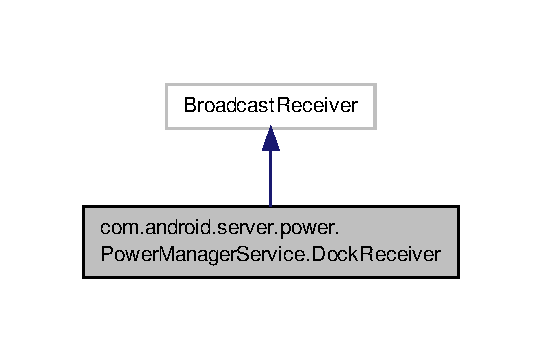
\includegraphics[width=260pt]{classcom_1_1android_1_1server_1_1power_1_1PowerManagerService_1_1DockReceiver__inherit__graph}
\end{center}
\end{figure}


Collaboration diagram for com.\-android.\-server.\-power.\-Power\-Manager\-Service.\-Dock\-Receiver\-:
\nopagebreak
\begin{figure}[H]
\begin{center}
\leavevmode
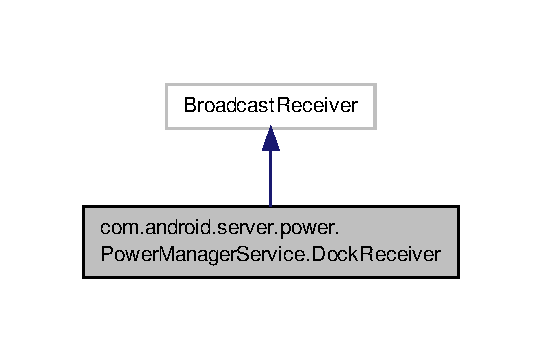
\includegraphics[width=260pt]{classcom_1_1android_1_1server_1_1power_1_1PowerManagerService_1_1DockReceiver__coll__graph}
\end{center}
\end{figure}
\subsection*{Public Member Functions}
\begin{DoxyCompactItemize}
\item 
void \hyperlink{classcom_1_1android_1_1server_1_1power_1_1PowerManagerService_1_1DockReceiver_a3334dd3d85872e0b85df18c73b2d4af7}{on\-Receive} (Context context, Intent intent)
\end{DoxyCompactItemize}


\subsection{Member Function Documentation}
\hypertarget{classcom_1_1android_1_1server_1_1power_1_1PowerManagerService_1_1DockReceiver_a3334dd3d85872e0b85df18c73b2d4af7}{\index{com\-::android\-::server\-::power\-::\-Power\-Manager\-Service\-::\-Dock\-Receiver@{com\-::android\-::server\-::power\-::\-Power\-Manager\-Service\-::\-Dock\-Receiver}!on\-Receive@{on\-Receive}}
\index{on\-Receive@{on\-Receive}!com::android::server::power::PowerManagerService::DockReceiver@{com\-::android\-::server\-::power\-::\-Power\-Manager\-Service\-::\-Dock\-Receiver}}
\subsubsection[{on\-Receive}]{\setlength{\rightskip}{0pt plus 5cm}void com.\-android.\-server.\-power.\-Power\-Manager\-Service.\-Dock\-Receiver.\-on\-Receive (
\begin{DoxyParamCaption}
\item[{Context}]{context, }
\item[{Intent}]{intent}
\end{DoxyParamCaption}
)\hspace{0.3cm}{\ttfamily [inline]}}}\label{classcom_1_1android_1_1server_1_1power_1_1PowerManagerService_1_1DockReceiver_a3334dd3d85872e0b85df18c73b2d4af7}


Here is the call graph for this function\-:
\nopagebreak
\begin{figure}[H]
\begin{center}
\leavevmode
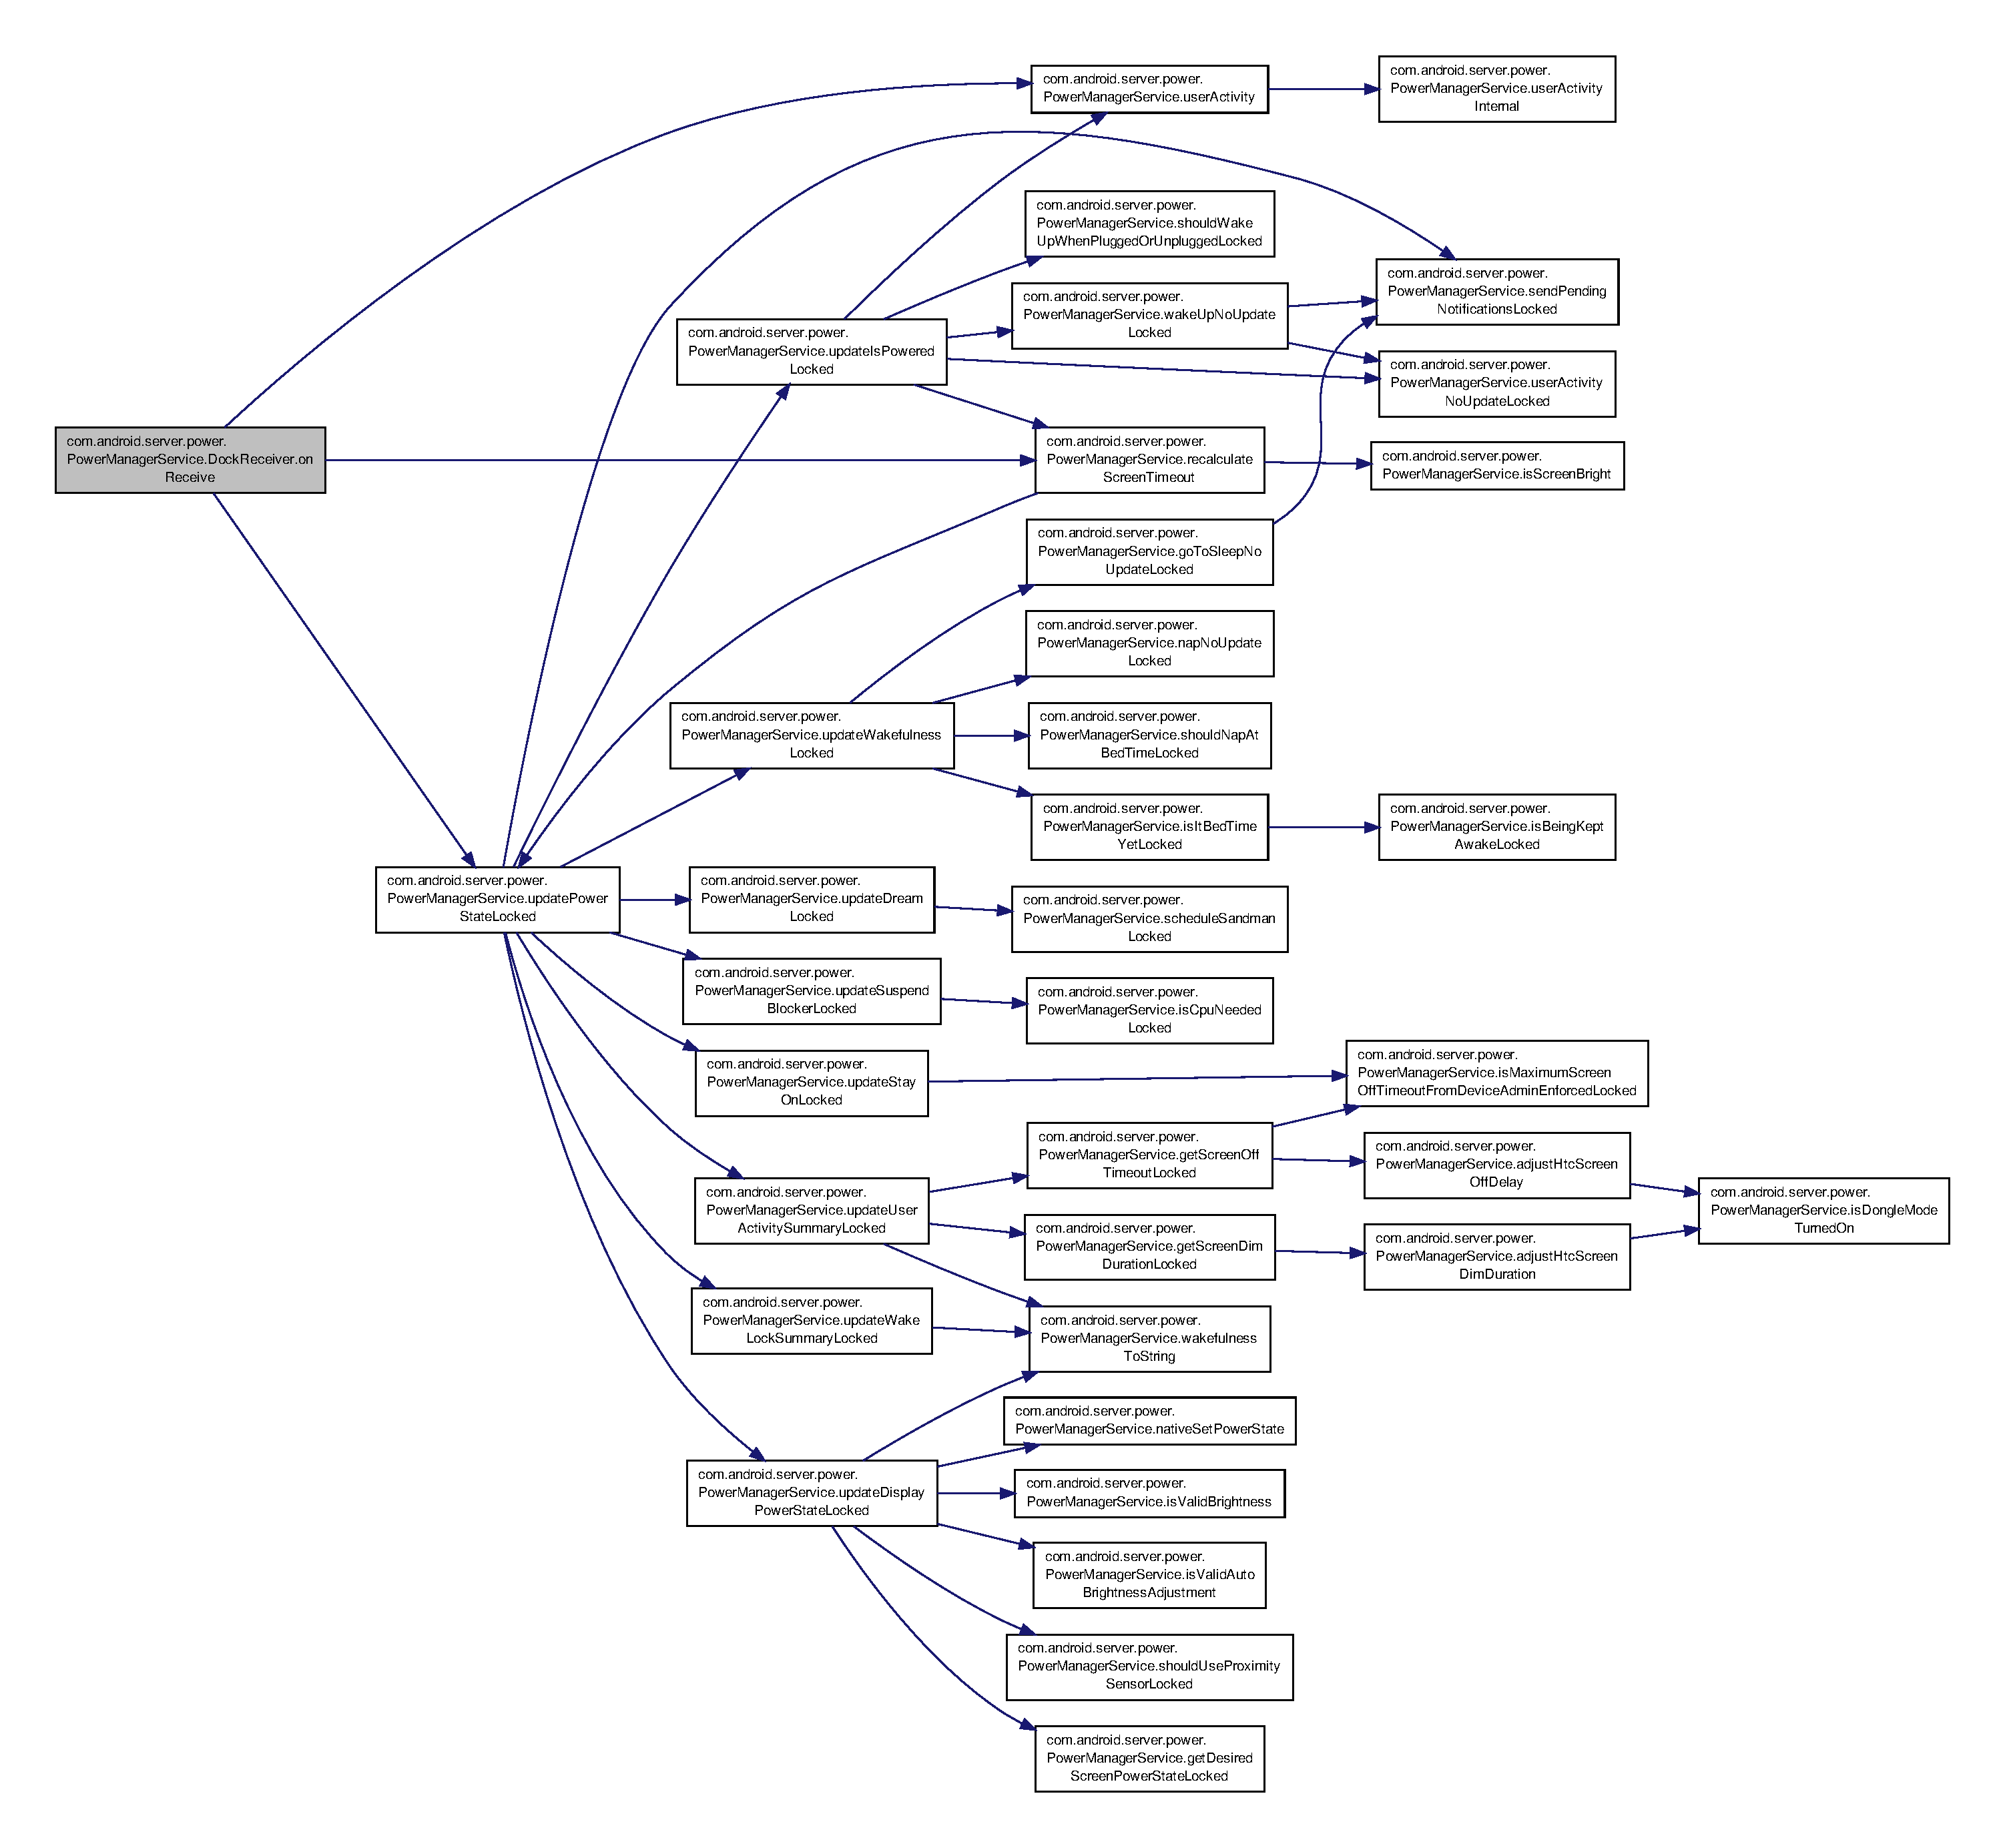
\includegraphics[width=350pt]{classcom_1_1android_1_1server_1_1power_1_1PowerManagerService_1_1DockReceiver_a3334dd3d85872e0b85df18c73b2d4af7_cgraph}
\end{center}
\end{figure}




The documentation for this class was generated from the following file\-:\begin{DoxyCompactItemize}
\item 
\hyperlink{PowerManagerService_8java}{Power\-Manager\-Service.\-java}\end{DoxyCompactItemize}

\hypertarget{classcom_1_1android_1_1server_1_1power_1_1DisplayPowerController_1_1DPCInternalAPI}{\section{com.\-android.\-server.\-power.\-Display\-Power\-Controller.\-D\-P\-C\-Internal\-A\-P\-I Class Reference}
\label{classcom_1_1android_1_1server_1_1power_1_1DisplayPowerController_1_1DPCInternalAPI}\index{com.\-android.\-server.\-power.\-Display\-Power\-Controller.\-D\-P\-C\-Internal\-A\-P\-I@{com.\-android.\-server.\-power.\-Display\-Power\-Controller.\-D\-P\-C\-Internal\-A\-P\-I}}
}
\subsection*{Protected Member Functions}
\begin{DoxyCompactItemize}
\item 
Spline \hyperlink{classcom_1_1android_1_1server_1_1power_1_1DisplayPowerController_1_1DPCInternalAPI_af719f1a4336338deff5689d39b774de6}{create\-Auto\-Brightness\-Spline} (int\mbox{[}$\,$\mbox{]} lux, int\mbox{[}$\,$\mbox{]} brightness)
\item 
void \hyperlink{classcom_1_1android_1_1server_1_1power_1_1DisplayPowerController_1_1DPCInternalAPI_a032004c23af272b086e9e5065e2447a5}{set\-Screen\-Brightness\-Mode} (int mode)
\item 
void \hyperlink{classcom_1_1android_1_1server_1_1power_1_1DisplayPowerController_1_1DPCInternalAPI_a3f131569d69c142341d26721af798574}{set\-Smooth\-Backlight} (int target\-Lcd\-Value, final int D\-U\-R\-A\-T\-I\-O\-N)
\item 
void \hyperlink{classcom_1_1android_1_1server_1_1power_1_1DisplayPowerController_1_1DPCInternalAPI_ab728f21a885e0c376a7f86406024fd87}{set\-Smooth\-Backlight\-For\-Camera} (int target\-Lcd\-Value, final int D\-U\-R\-A\-T\-I\-O\-N)
\item 
int \hyperlink{classcom_1_1android_1_1server_1_1power_1_1DisplayPowerController_1_1DPCInternalAPI_a0abf8f35bf3eaf286550fb4c4b8fa7bc}{get\-Current\-Brightness} ()
\item 
int \hyperlink{classcom_1_1android_1_1server_1_1power_1_1DisplayPowerController_1_1DPCInternalAPI_a4befd48a2deb6b135f55023cc34af003}{get\-Target\-Brightness} ()
\item 
void \hyperlink{classcom_1_1android_1_1server_1_1power_1_1DisplayPowerController_1_1DPCInternalAPI_a477f8db4ee8812198a20317c9bd8bb4f}{cancel\-Animation} ()
\item 
void \hyperlink{classcom_1_1android_1_1server_1_1power_1_1DisplayPowerController_1_1DPCInternalAPI_ad6c47e948ab63bc51cb6bbbf8331783e}{force\-Brightness\-Update} (final int D\-U\-R\-A\-T\-I\-O\-N)
\item 
void \hyperlink{classcom_1_1android_1_1server_1_1power_1_1DisplayPowerController_1_1DPCInternalAPI_a09aab6ed7aac7d7162bcac97e12da3fe}{send\-Update\-Power\-State} ()
\end{DoxyCompactItemize}
\subsection*{Private Member Functions}
\begin{DoxyCompactItemize}
\item 
\hyperlink{classcom_1_1android_1_1server_1_1power_1_1DisplayPowerController_1_1DPCInternalAPI_a2e7bfff67ec579b43f899138704f0e23}{D\-P\-C\-Internal\-A\-P\-I} ()
\end{DoxyCompactItemize}


\subsection{Constructor \& Destructor Documentation}
\hypertarget{classcom_1_1android_1_1server_1_1power_1_1DisplayPowerController_1_1DPCInternalAPI_a2e7bfff67ec579b43f899138704f0e23}{\index{com\-::android\-::server\-::power\-::\-Display\-Power\-Controller\-::\-D\-P\-C\-Internal\-A\-P\-I@{com\-::android\-::server\-::power\-::\-Display\-Power\-Controller\-::\-D\-P\-C\-Internal\-A\-P\-I}!D\-P\-C\-Internal\-A\-P\-I@{D\-P\-C\-Internal\-A\-P\-I}}
\index{D\-P\-C\-Internal\-A\-P\-I@{D\-P\-C\-Internal\-A\-P\-I}!com::android::server::power::DisplayPowerController::DPCInternalAPI@{com\-::android\-::server\-::power\-::\-Display\-Power\-Controller\-::\-D\-P\-C\-Internal\-A\-P\-I}}
\subsubsection[{D\-P\-C\-Internal\-A\-P\-I}]{\setlength{\rightskip}{0pt plus 5cm}com.\-android.\-server.\-power.\-Display\-Power\-Controller.\-D\-P\-C\-Internal\-A\-P\-I.\-D\-P\-C\-Internal\-A\-P\-I (
\begin{DoxyParamCaption}
{}
\end{DoxyParamCaption}
)\hspace{0.3cm}{\ttfamily [inline]}, {\ttfamily [private]}}}\label{classcom_1_1android_1_1server_1_1power_1_1DisplayPowerController_1_1DPCInternalAPI_a2e7bfff67ec579b43f899138704f0e23}


\subsection{Member Function Documentation}
\hypertarget{classcom_1_1android_1_1server_1_1power_1_1DisplayPowerController_1_1DPCInternalAPI_a477f8db4ee8812198a20317c9bd8bb4f}{\index{com\-::android\-::server\-::power\-::\-Display\-Power\-Controller\-::\-D\-P\-C\-Internal\-A\-P\-I@{com\-::android\-::server\-::power\-::\-Display\-Power\-Controller\-::\-D\-P\-C\-Internal\-A\-P\-I}!cancel\-Animation@{cancel\-Animation}}
\index{cancel\-Animation@{cancel\-Animation}!com::android::server::power::DisplayPowerController::DPCInternalAPI@{com\-::android\-::server\-::power\-::\-Display\-Power\-Controller\-::\-D\-P\-C\-Internal\-A\-P\-I}}
\subsubsection[{cancel\-Animation}]{\setlength{\rightskip}{0pt plus 5cm}void com.\-android.\-server.\-power.\-Display\-Power\-Controller.\-D\-P\-C\-Internal\-A\-P\-I.\-cancel\-Animation (
\begin{DoxyParamCaption}
{}
\end{DoxyParamCaption}
)\hspace{0.3cm}{\ttfamily [inline]}, {\ttfamily [protected]}}}\label{classcom_1_1android_1_1server_1_1power_1_1DisplayPowerController_1_1DPCInternalAPI_a477f8db4ee8812198a20317c9bd8bb4f}
\hypertarget{classcom_1_1android_1_1server_1_1power_1_1DisplayPowerController_1_1DPCInternalAPI_af719f1a4336338deff5689d39b774de6}{\index{com\-::android\-::server\-::power\-::\-Display\-Power\-Controller\-::\-D\-P\-C\-Internal\-A\-P\-I@{com\-::android\-::server\-::power\-::\-Display\-Power\-Controller\-::\-D\-P\-C\-Internal\-A\-P\-I}!create\-Auto\-Brightness\-Spline@{create\-Auto\-Brightness\-Spline}}
\index{create\-Auto\-Brightness\-Spline@{create\-Auto\-Brightness\-Spline}!com::android::server::power::DisplayPowerController::DPCInternalAPI@{com\-::android\-::server\-::power\-::\-Display\-Power\-Controller\-::\-D\-P\-C\-Internal\-A\-P\-I}}
\subsubsection[{create\-Auto\-Brightness\-Spline}]{\setlength{\rightskip}{0pt plus 5cm}Spline com.\-android.\-server.\-power.\-Display\-Power\-Controller.\-D\-P\-C\-Internal\-A\-P\-I.\-create\-Auto\-Brightness\-Spline (
\begin{DoxyParamCaption}
\item[{int\mbox{[}$\,$\mbox{]}}]{lux, }
\item[{int\mbox{[}$\,$\mbox{]}}]{brightness}
\end{DoxyParamCaption}
)\hspace{0.3cm}{\ttfamily [inline]}, {\ttfamily [protected]}}}\label{classcom_1_1android_1_1server_1_1power_1_1DisplayPowerController_1_1DPCInternalAPI_af719f1a4336338deff5689d39b774de6}
\hypertarget{classcom_1_1android_1_1server_1_1power_1_1DisplayPowerController_1_1DPCInternalAPI_ad6c47e948ab63bc51cb6bbbf8331783e}{\index{com\-::android\-::server\-::power\-::\-Display\-Power\-Controller\-::\-D\-P\-C\-Internal\-A\-P\-I@{com\-::android\-::server\-::power\-::\-Display\-Power\-Controller\-::\-D\-P\-C\-Internal\-A\-P\-I}!force\-Brightness\-Update@{force\-Brightness\-Update}}
\index{force\-Brightness\-Update@{force\-Brightness\-Update}!com::android::server::power::DisplayPowerController::DPCInternalAPI@{com\-::android\-::server\-::power\-::\-Display\-Power\-Controller\-::\-D\-P\-C\-Internal\-A\-P\-I}}
\subsubsection[{force\-Brightness\-Update}]{\setlength{\rightskip}{0pt plus 5cm}void com.\-android.\-server.\-power.\-Display\-Power\-Controller.\-D\-P\-C\-Internal\-A\-P\-I.\-force\-Brightness\-Update (
\begin{DoxyParamCaption}
\item[{final int}]{D\-U\-R\-A\-T\-I\-O\-N}
\end{DoxyParamCaption}
)\hspace{0.3cm}{\ttfamily [inline]}, {\ttfamily [protected]}}}\label{classcom_1_1android_1_1server_1_1power_1_1DisplayPowerController_1_1DPCInternalAPI_ad6c47e948ab63bc51cb6bbbf8331783e}
\hypertarget{classcom_1_1android_1_1server_1_1power_1_1DisplayPowerController_1_1DPCInternalAPI_a0abf8f35bf3eaf286550fb4c4b8fa7bc}{\index{com\-::android\-::server\-::power\-::\-Display\-Power\-Controller\-::\-D\-P\-C\-Internal\-A\-P\-I@{com\-::android\-::server\-::power\-::\-Display\-Power\-Controller\-::\-D\-P\-C\-Internal\-A\-P\-I}!get\-Current\-Brightness@{get\-Current\-Brightness}}
\index{get\-Current\-Brightness@{get\-Current\-Brightness}!com::android::server::power::DisplayPowerController::DPCInternalAPI@{com\-::android\-::server\-::power\-::\-Display\-Power\-Controller\-::\-D\-P\-C\-Internal\-A\-P\-I}}
\subsubsection[{get\-Current\-Brightness}]{\setlength{\rightskip}{0pt plus 5cm}int com.\-android.\-server.\-power.\-Display\-Power\-Controller.\-D\-P\-C\-Internal\-A\-P\-I.\-get\-Current\-Brightness (
\begin{DoxyParamCaption}
{}
\end{DoxyParamCaption}
)\hspace{0.3cm}{\ttfamily [inline]}, {\ttfamily [protected]}}}\label{classcom_1_1android_1_1server_1_1power_1_1DisplayPowerController_1_1DPCInternalAPI_a0abf8f35bf3eaf286550fb4c4b8fa7bc}
\hypertarget{classcom_1_1android_1_1server_1_1power_1_1DisplayPowerController_1_1DPCInternalAPI_a4befd48a2deb6b135f55023cc34af003}{\index{com\-::android\-::server\-::power\-::\-Display\-Power\-Controller\-::\-D\-P\-C\-Internal\-A\-P\-I@{com\-::android\-::server\-::power\-::\-Display\-Power\-Controller\-::\-D\-P\-C\-Internal\-A\-P\-I}!get\-Target\-Brightness@{get\-Target\-Brightness}}
\index{get\-Target\-Brightness@{get\-Target\-Brightness}!com::android::server::power::DisplayPowerController::DPCInternalAPI@{com\-::android\-::server\-::power\-::\-Display\-Power\-Controller\-::\-D\-P\-C\-Internal\-A\-P\-I}}
\subsubsection[{get\-Target\-Brightness}]{\setlength{\rightskip}{0pt plus 5cm}int com.\-android.\-server.\-power.\-Display\-Power\-Controller.\-D\-P\-C\-Internal\-A\-P\-I.\-get\-Target\-Brightness (
\begin{DoxyParamCaption}
{}
\end{DoxyParamCaption}
)\hspace{0.3cm}{\ttfamily [inline]}, {\ttfamily [protected]}}}\label{classcom_1_1android_1_1server_1_1power_1_1DisplayPowerController_1_1DPCInternalAPI_a4befd48a2deb6b135f55023cc34af003}
\hypertarget{classcom_1_1android_1_1server_1_1power_1_1DisplayPowerController_1_1DPCInternalAPI_a09aab6ed7aac7d7162bcac97e12da3fe}{\index{com\-::android\-::server\-::power\-::\-Display\-Power\-Controller\-::\-D\-P\-C\-Internal\-A\-P\-I@{com\-::android\-::server\-::power\-::\-Display\-Power\-Controller\-::\-D\-P\-C\-Internal\-A\-P\-I}!send\-Update\-Power\-State@{send\-Update\-Power\-State}}
\index{send\-Update\-Power\-State@{send\-Update\-Power\-State}!com::android::server::power::DisplayPowerController::DPCInternalAPI@{com\-::android\-::server\-::power\-::\-Display\-Power\-Controller\-::\-D\-P\-C\-Internal\-A\-P\-I}}
\subsubsection[{send\-Update\-Power\-State}]{\setlength{\rightskip}{0pt plus 5cm}void com.\-android.\-server.\-power.\-Display\-Power\-Controller.\-D\-P\-C\-Internal\-A\-P\-I.\-send\-Update\-Power\-State (
\begin{DoxyParamCaption}
{}
\end{DoxyParamCaption}
)\hspace{0.3cm}{\ttfamily [inline]}, {\ttfamily [protected]}}}\label{classcom_1_1android_1_1server_1_1power_1_1DisplayPowerController_1_1DPCInternalAPI_a09aab6ed7aac7d7162bcac97e12da3fe}
\hypertarget{classcom_1_1android_1_1server_1_1power_1_1DisplayPowerController_1_1DPCInternalAPI_a032004c23af272b086e9e5065e2447a5}{\index{com\-::android\-::server\-::power\-::\-Display\-Power\-Controller\-::\-D\-P\-C\-Internal\-A\-P\-I@{com\-::android\-::server\-::power\-::\-Display\-Power\-Controller\-::\-D\-P\-C\-Internal\-A\-P\-I}!set\-Screen\-Brightness\-Mode@{set\-Screen\-Brightness\-Mode}}
\index{set\-Screen\-Brightness\-Mode@{set\-Screen\-Brightness\-Mode}!com::android::server::power::DisplayPowerController::DPCInternalAPI@{com\-::android\-::server\-::power\-::\-Display\-Power\-Controller\-::\-D\-P\-C\-Internal\-A\-P\-I}}
\subsubsection[{set\-Screen\-Brightness\-Mode}]{\setlength{\rightskip}{0pt plus 5cm}void com.\-android.\-server.\-power.\-Display\-Power\-Controller.\-D\-P\-C\-Internal\-A\-P\-I.\-set\-Screen\-Brightness\-Mode (
\begin{DoxyParamCaption}
\item[{int}]{mode}
\end{DoxyParamCaption}
)\hspace{0.3cm}{\ttfamily [inline]}, {\ttfamily [protected]}}}\label{classcom_1_1android_1_1server_1_1power_1_1DisplayPowerController_1_1DPCInternalAPI_a032004c23af272b086e9e5065e2447a5}
\hypertarget{classcom_1_1android_1_1server_1_1power_1_1DisplayPowerController_1_1DPCInternalAPI_a3f131569d69c142341d26721af798574}{\index{com\-::android\-::server\-::power\-::\-Display\-Power\-Controller\-::\-D\-P\-C\-Internal\-A\-P\-I@{com\-::android\-::server\-::power\-::\-Display\-Power\-Controller\-::\-D\-P\-C\-Internal\-A\-P\-I}!set\-Smooth\-Backlight@{set\-Smooth\-Backlight}}
\index{set\-Smooth\-Backlight@{set\-Smooth\-Backlight}!com::android::server::power::DisplayPowerController::DPCInternalAPI@{com\-::android\-::server\-::power\-::\-Display\-Power\-Controller\-::\-D\-P\-C\-Internal\-A\-P\-I}}
\subsubsection[{set\-Smooth\-Backlight}]{\setlength{\rightskip}{0pt plus 5cm}void com.\-android.\-server.\-power.\-Display\-Power\-Controller.\-D\-P\-C\-Internal\-A\-P\-I.\-set\-Smooth\-Backlight (
\begin{DoxyParamCaption}
\item[{int}]{target\-Lcd\-Value, }
\item[{final int}]{D\-U\-R\-A\-T\-I\-O\-N}
\end{DoxyParamCaption}
)\hspace{0.3cm}{\ttfamily [inline]}, {\ttfamily [protected]}}}\label{classcom_1_1android_1_1server_1_1power_1_1DisplayPowerController_1_1DPCInternalAPI_a3f131569d69c142341d26721af798574}
\hypertarget{classcom_1_1android_1_1server_1_1power_1_1DisplayPowerController_1_1DPCInternalAPI_ab728f21a885e0c376a7f86406024fd87}{\index{com\-::android\-::server\-::power\-::\-Display\-Power\-Controller\-::\-D\-P\-C\-Internal\-A\-P\-I@{com\-::android\-::server\-::power\-::\-Display\-Power\-Controller\-::\-D\-P\-C\-Internal\-A\-P\-I}!set\-Smooth\-Backlight\-For\-Camera@{set\-Smooth\-Backlight\-For\-Camera}}
\index{set\-Smooth\-Backlight\-For\-Camera@{set\-Smooth\-Backlight\-For\-Camera}!com::android::server::power::DisplayPowerController::DPCInternalAPI@{com\-::android\-::server\-::power\-::\-Display\-Power\-Controller\-::\-D\-P\-C\-Internal\-A\-P\-I}}
\subsubsection[{set\-Smooth\-Backlight\-For\-Camera}]{\setlength{\rightskip}{0pt plus 5cm}void com.\-android.\-server.\-power.\-Display\-Power\-Controller.\-D\-P\-C\-Internal\-A\-P\-I.\-set\-Smooth\-Backlight\-For\-Camera (
\begin{DoxyParamCaption}
\item[{int}]{target\-Lcd\-Value, }
\item[{final int}]{D\-U\-R\-A\-T\-I\-O\-N}
\end{DoxyParamCaption}
)\hspace{0.3cm}{\ttfamily [inline]}, {\ttfamily [protected]}}}\label{classcom_1_1android_1_1server_1_1power_1_1DisplayPowerController_1_1DPCInternalAPI_ab728f21a885e0c376a7f86406024fd87}


The documentation for this class was generated from the following file\-:\begin{DoxyCompactItemize}
\item 
\hyperlink{DisplayPowerController_8java}{Display\-Power\-Controller.\-java}\end{DoxyCompactItemize}

\hypertarget{classcom_1_1android_1_1server_1_1power_1_1PowerManagerService_1_1DreamReceiver}{\section{com.\-android.\-server.\-power.\-Power\-Manager\-Service.\-Dream\-Receiver Class Reference}
\label{classcom_1_1android_1_1server_1_1power_1_1PowerManagerService_1_1DreamReceiver}\index{com.\-android.\-server.\-power.\-Power\-Manager\-Service.\-Dream\-Receiver@{com.\-android.\-server.\-power.\-Power\-Manager\-Service.\-Dream\-Receiver}}
}


Inheritance diagram for com.\-android.\-server.\-power.\-Power\-Manager\-Service.\-Dream\-Receiver\-:
\nopagebreak
\begin{figure}[H]
\begin{center}
\leavevmode
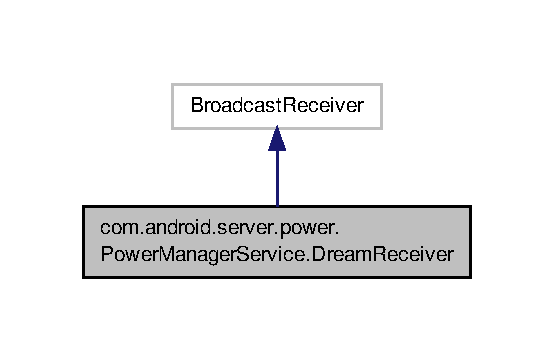
\includegraphics[width=266pt]{classcom_1_1android_1_1server_1_1power_1_1PowerManagerService_1_1DreamReceiver__inherit__graph}
\end{center}
\end{figure}


Collaboration diagram for com.\-android.\-server.\-power.\-Power\-Manager\-Service.\-Dream\-Receiver\-:
\nopagebreak
\begin{figure}[H]
\begin{center}
\leavevmode
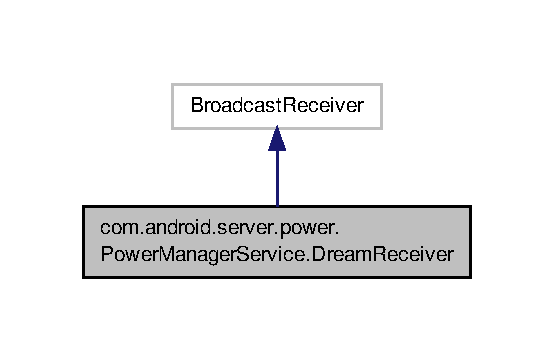
\includegraphics[width=266pt]{classcom_1_1android_1_1server_1_1power_1_1PowerManagerService_1_1DreamReceiver__coll__graph}
\end{center}
\end{figure}
\subsection*{Public Member Functions}
\begin{DoxyCompactItemize}
\item 
void \hyperlink{classcom_1_1android_1_1server_1_1power_1_1PowerManagerService_1_1DreamReceiver_a8169511c78f4f75ffac9433b94dfec31}{on\-Receive} (Context context, Intent intent)
\end{DoxyCompactItemize}


\subsection{Member Function Documentation}
\hypertarget{classcom_1_1android_1_1server_1_1power_1_1PowerManagerService_1_1DreamReceiver_a8169511c78f4f75ffac9433b94dfec31}{\index{com\-::android\-::server\-::power\-::\-Power\-Manager\-Service\-::\-Dream\-Receiver@{com\-::android\-::server\-::power\-::\-Power\-Manager\-Service\-::\-Dream\-Receiver}!on\-Receive@{on\-Receive}}
\index{on\-Receive@{on\-Receive}!com::android::server::power::PowerManagerService::DreamReceiver@{com\-::android\-::server\-::power\-::\-Power\-Manager\-Service\-::\-Dream\-Receiver}}
\subsubsection[{on\-Receive}]{\setlength{\rightskip}{0pt plus 5cm}void com.\-android.\-server.\-power.\-Power\-Manager\-Service.\-Dream\-Receiver.\-on\-Receive (
\begin{DoxyParamCaption}
\item[{Context}]{context, }
\item[{Intent}]{intent}
\end{DoxyParamCaption}
)\hspace{0.3cm}{\ttfamily [inline]}}}\label{classcom_1_1android_1_1server_1_1power_1_1PowerManagerService_1_1DreamReceiver_a8169511c78f4f75ffac9433b94dfec31}


Here is the call graph for this function\-:
\nopagebreak
\begin{figure}[H]
\begin{center}
\leavevmode
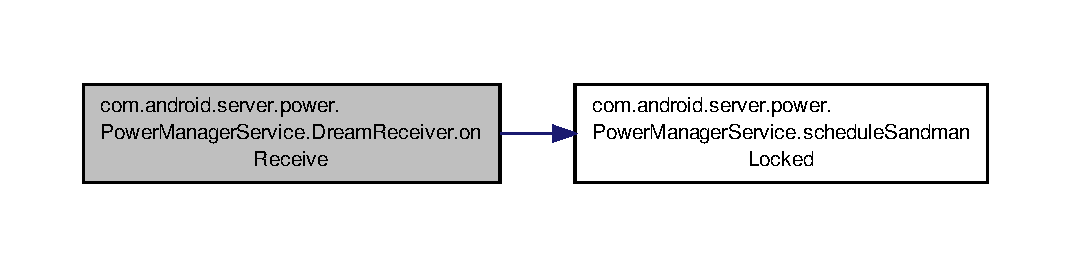
\includegraphics[width=350pt]{classcom_1_1android_1_1server_1_1power_1_1PowerManagerService_1_1DreamReceiver_a8169511c78f4f75ffac9433b94dfec31_cgraph}
\end{center}
\end{figure}




The documentation for this class was generated from the following file\-:\begin{DoxyCompactItemize}
\item 
\hyperlink{PowerManagerService_8java}{Power\-Manager\-Service.\-java}\end{DoxyCompactItemize}

\hypertarget{classcom_1_1android_1_1server_1_1power_1_1PowerManagerService_1_1HtcCpuCtrl}{\section{com.\-android.\-server.\-power.\-Power\-Manager\-Service.\-Htc\-Cpu\-Ctrl Class Reference}
\label{classcom_1_1android_1_1server_1_1power_1_1PowerManagerService_1_1HtcCpuCtrl}\index{com.\-android.\-server.\-power.\-Power\-Manager\-Service.\-Htc\-Cpu\-Ctrl@{com.\-android.\-server.\-power.\-Power\-Manager\-Service.\-Htc\-Cpu\-Ctrl}}
}


Inheritance diagram for com.\-android.\-server.\-power.\-Power\-Manager\-Service.\-Htc\-Cpu\-Ctrl\-:
\nopagebreak
\begin{figure}[H]
\begin{center}
\leavevmode
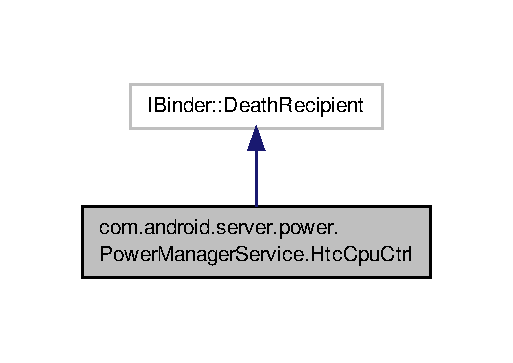
\includegraphics[width=246pt]{classcom_1_1android_1_1server_1_1power_1_1PowerManagerService_1_1HtcCpuCtrl__inherit__graph}
\end{center}
\end{figure}


Collaboration diagram for com.\-android.\-server.\-power.\-Power\-Manager\-Service.\-Htc\-Cpu\-Ctrl\-:
\nopagebreak
\begin{figure}[H]
\begin{center}
\leavevmode
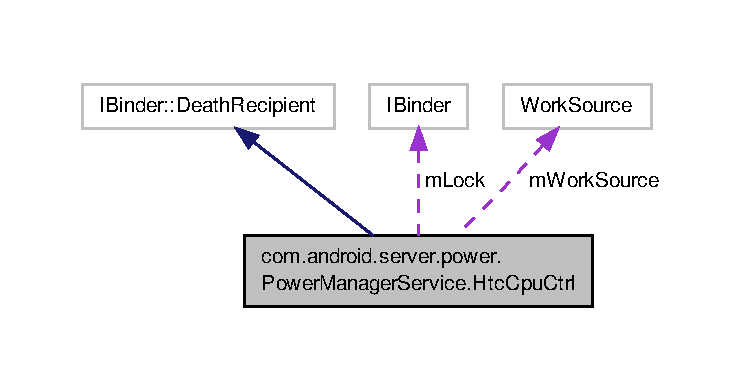
\includegraphics[width=350pt]{classcom_1_1android_1_1server_1_1power_1_1PowerManagerService_1_1HtcCpuCtrl__coll__graph}
\end{center}
\end{figure}
\subsection*{Public Member Functions}
\begin{DoxyCompactItemize}
\item 
\hyperlink{classcom_1_1android_1_1server_1_1power_1_1PowerManagerService_1_1HtcCpuCtrl_a7bd3fe868e78e2744c6b03a40e01128c}{Htc\-Cpu\-Ctrl} (I\-Binder lock, int flags, String tag, Work\-Source work\-Source, int owner\-Uid, int owner\-Pid, int level)
\item 
int \hyperlink{classcom_1_1android_1_1server_1_1power_1_1PowerManagerService_1_1HtcCpuCtrl_ada5ade08fc1bbc694eb3fbad8238102c}{get\-Level} ()
\item 
void \hyperlink{classcom_1_1android_1_1server_1_1power_1_1PowerManagerService_1_1HtcCpuCtrl_a74f222d6908370d9129ee780050df1e9}{binder\-Died} ()
\item 
boolean \hyperlink{classcom_1_1android_1_1server_1_1power_1_1PowerManagerService_1_1HtcCpuCtrl_a7da367150c7c4506ceffbac3283ee7e9}{has\-Same\-Properties} (int flags, String tag, Work\-Source work\-Source, int owner\-Uid, int owner\-Pid)
\item 
void \hyperlink{classcom_1_1android_1_1server_1_1power_1_1PowerManagerService_1_1HtcCpuCtrl_a97aaf5d3af48928c73af170a64a869b3}{update\-Properties} (int flags, String tag, Work\-Source work\-Source, int owner\-Uid, int owner\-Pid)
\item 
boolean \hyperlink{classcom_1_1android_1_1server_1_1power_1_1PowerManagerService_1_1HtcCpuCtrl_a31b1cc24bd6f3624ad1a71eafe2fad64}{has\-Same\-Work\-Source} (Work\-Source work\-Source)
\item 
void \hyperlink{classcom_1_1android_1_1server_1_1power_1_1PowerManagerService_1_1HtcCpuCtrl_abd81472be2ab5e7eccc8c68840b3bbfa}{update\-Work\-Source} (Work\-Source work\-Source)
\item 
String \hyperlink{classcom_1_1android_1_1server_1_1power_1_1PowerManagerService_1_1HtcCpuCtrl_a2e8197ca6777001ab61ab5ce23db7907}{to\-String} ()
\item 
String \hyperlink{classcom_1_1android_1_1server_1_1power_1_1PowerManagerService_1_1HtcCpuCtrl_a71169bb582d98e91065617e46be5dd03}{cpu\-Freq\-Level\-To\-String} ()
\item 
String \hyperlink{classcom_1_1android_1_1server_1_1power_1_1PowerManagerService_1_1HtcCpuCtrl_a1e5118d0b28e0b0bc81dbb3247b9c567}{cpu\-Num\-Level\-To\-String} ()
\end{DoxyCompactItemize}
\subsection*{Public Attributes}
\begin{DoxyCompactItemize}
\item 
final I\-Binder \hyperlink{classcom_1_1android_1_1server_1_1power_1_1PowerManagerService_1_1HtcCpuCtrl_a9c26de2babb8433dad620487e6da90ee}{m\-Lock}
\item 
int \hyperlink{classcom_1_1android_1_1server_1_1power_1_1PowerManagerService_1_1HtcCpuCtrl_a9658c794544e425656117e195286043f}{m\-Flags}
\item 
String \hyperlink{classcom_1_1android_1_1server_1_1power_1_1PowerManagerService_1_1HtcCpuCtrl_acd2763c41cf2375b632557850fa9f0cd}{m\-Tag}
\item 
Work\-Source \hyperlink{classcom_1_1android_1_1server_1_1power_1_1PowerManagerService_1_1HtcCpuCtrl_a29942ea13180d98f1a9e4ea444834d1b}{m\-Work\-Source}
\item 
int \hyperlink{classcom_1_1android_1_1server_1_1power_1_1PowerManagerService_1_1HtcCpuCtrl_ac14893ba75fd5aa8d1d1c7173adb90a0}{m\-Owner\-Uid}
\item 
int \hyperlink{classcom_1_1android_1_1server_1_1power_1_1PowerManagerService_1_1HtcCpuCtrl_adf0bb931ec82c6a5b68d8b2ab0c451b1}{m\-Owner\-Pid}
\end{DoxyCompactItemize}
\subsection*{Private Member Functions}
\begin{DoxyCompactItemize}
\item 
String \hyperlink{classcom_1_1android_1_1server_1_1power_1_1PowerManagerService_1_1HtcCpuCtrl_a56baa8905bc9d8a055b65b8a4f86a4fc}{get\-Lock\-Level\-String} ()
\item 
String \hyperlink{classcom_1_1android_1_1server_1_1power_1_1PowerManagerService_1_1HtcCpuCtrl_a095dd0137eb8fdb5155505205400d0c9}{dump\-Level\-If\-Exist} ()
\end{DoxyCompactItemize}
\subsection*{Private Attributes}
\begin{DoxyCompactItemize}
\item 
int \hyperlink{classcom_1_1android_1_1server_1_1power_1_1PowerManagerService_1_1HtcCpuCtrl_a6a210dc8e827717053a51bf27c637e0b}{m\-Level}
\end{DoxyCompactItemize}


\subsection{Constructor \& Destructor Documentation}
\hypertarget{classcom_1_1android_1_1server_1_1power_1_1PowerManagerService_1_1HtcCpuCtrl_a7bd3fe868e78e2744c6b03a40e01128c}{\index{com\-::android\-::server\-::power\-::\-Power\-Manager\-Service\-::\-Htc\-Cpu\-Ctrl@{com\-::android\-::server\-::power\-::\-Power\-Manager\-Service\-::\-Htc\-Cpu\-Ctrl}!Htc\-Cpu\-Ctrl@{Htc\-Cpu\-Ctrl}}
\index{Htc\-Cpu\-Ctrl@{Htc\-Cpu\-Ctrl}!com::android::server::power::PowerManagerService::HtcCpuCtrl@{com\-::android\-::server\-::power\-::\-Power\-Manager\-Service\-::\-Htc\-Cpu\-Ctrl}}
\subsubsection[{Htc\-Cpu\-Ctrl}]{\setlength{\rightskip}{0pt plus 5cm}com.\-android.\-server.\-power.\-Power\-Manager\-Service.\-Htc\-Cpu\-Ctrl.\-Htc\-Cpu\-Ctrl (
\begin{DoxyParamCaption}
\item[{I\-Binder}]{lock, }
\item[{int}]{flags, }
\item[{String}]{tag, }
\item[{Work\-Source}]{work\-Source, }
\item[{int}]{owner\-Uid, }
\item[{int}]{owner\-Pid, }
\item[{int}]{level}
\end{DoxyParamCaption}
)\hspace{0.3cm}{\ttfamily [inline]}}}\label{classcom_1_1android_1_1server_1_1power_1_1PowerManagerService_1_1HtcCpuCtrl_a7bd3fe868e78e2744c6b03a40e01128c}


Here is the call graph for this function\-:
\nopagebreak
\begin{figure}[H]
\begin{center}
\leavevmode
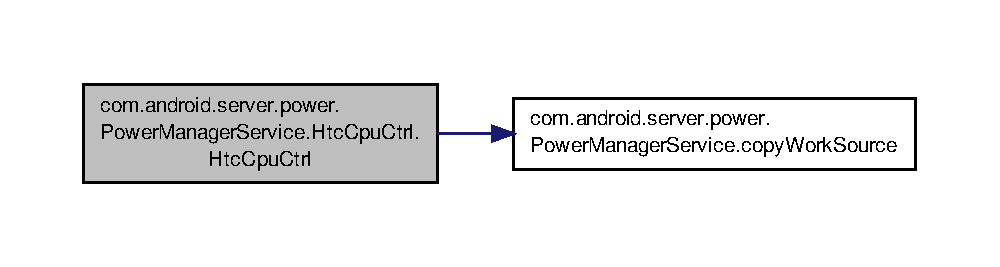
\includegraphics[width=350pt]{classcom_1_1android_1_1server_1_1power_1_1PowerManagerService_1_1HtcCpuCtrl_a7bd3fe868e78e2744c6b03a40e01128c_cgraph}
\end{center}
\end{figure}




\subsection{Member Function Documentation}
\hypertarget{classcom_1_1android_1_1server_1_1power_1_1PowerManagerService_1_1HtcCpuCtrl_a74f222d6908370d9129ee780050df1e9}{\index{com\-::android\-::server\-::power\-::\-Power\-Manager\-Service\-::\-Htc\-Cpu\-Ctrl@{com\-::android\-::server\-::power\-::\-Power\-Manager\-Service\-::\-Htc\-Cpu\-Ctrl}!binder\-Died@{binder\-Died}}
\index{binder\-Died@{binder\-Died}!com::android::server::power::PowerManagerService::HtcCpuCtrl@{com\-::android\-::server\-::power\-::\-Power\-Manager\-Service\-::\-Htc\-Cpu\-Ctrl}}
\subsubsection[{binder\-Died}]{\setlength{\rightskip}{0pt plus 5cm}void com.\-android.\-server.\-power.\-Power\-Manager\-Service.\-Htc\-Cpu\-Ctrl.\-binder\-Died (
\begin{DoxyParamCaption}
{}
\end{DoxyParamCaption}
)\hspace{0.3cm}{\ttfamily [inline]}}}\label{classcom_1_1android_1_1server_1_1power_1_1PowerManagerService_1_1HtcCpuCtrl_a74f222d6908370d9129ee780050df1e9}
\hypertarget{classcom_1_1android_1_1server_1_1power_1_1PowerManagerService_1_1HtcCpuCtrl_a71169bb582d98e91065617e46be5dd03}{\index{com\-::android\-::server\-::power\-::\-Power\-Manager\-Service\-::\-Htc\-Cpu\-Ctrl@{com\-::android\-::server\-::power\-::\-Power\-Manager\-Service\-::\-Htc\-Cpu\-Ctrl}!cpu\-Freq\-Level\-To\-String@{cpu\-Freq\-Level\-To\-String}}
\index{cpu\-Freq\-Level\-To\-String@{cpu\-Freq\-Level\-To\-String}!com::android::server::power::PowerManagerService::HtcCpuCtrl@{com\-::android\-::server\-::power\-::\-Power\-Manager\-Service\-::\-Htc\-Cpu\-Ctrl}}
\subsubsection[{cpu\-Freq\-Level\-To\-String}]{\setlength{\rightskip}{0pt plus 5cm}String com.\-android.\-server.\-power.\-Power\-Manager\-Service.\-Htc\-Cpu\-Ctrl.\-cpu\-Freq\-Level\-To\-String (
\begin{DoxyParamCaption}
{}
\end{DoxyParamCaption}
)\hspace{0.3cm}{\ttfamily [inline]}}}\label{classcom_1_1android_1_1server_1_1power_1_1PowerManagerService_1_1HtcCpuCtrl_a71169bb582d98e91065617e46be5dd03}
\hypertarget{classcom_1_1android_1_1server_1_1power_1_1PowerManagerService_1_1HtcCpuCtrl_a1e5118d0b28e0b0bc81dbb3247b9c567}{\index{com\-::android\-::server\-::power\-::\-Power\-Manager\-Service\-::\-Htc\-Cpu\-Ctrl@{com\-::android\-::server\-::power\-::\-Power\-Manager\-Service\-::\-Htc\-Cpu\-Ctrl}!cpu\-Num\-Level\-To\-String@{cpu\-Num\-Level\-To\-String}}
\index{cpu\-Num\-Level\-To\-String@{cpu\-Num\-Level\-To\-String}!com::android::server::power::PowerManagerService::HtcCpuCtrl@{com\-::android\-::server\-::power\-::\-Power\-Manager\-Service\-::\-Htc\-Cpu\-Ctrl}}
\subsubsection[{cpu\-Num\-Level\-To\-String}]{\setlength{\rightskip}{0pt plus 5cm}String com.\-android.\-server.\-power.\-Power\-Manager\-Service.\-Htc\-Cpu\-Ctrl.\-cpu\-Num\-Level\-To\-String (
\begin{DoxyParamCaption}
{}
\end{DoxyParamCaption}
)\hspace{0.3cm}{\ttfamily [inline]}}}\label{classcom_1_1android_1_1server_1_1power_1_1PowerManagerService_1_1HtcCpuCtrl_a1e5118d0b28e0b0bc81dbb3247b9c567}
\hypertarget{classcom_1_1android_1_1server_1_1power_1_1PowerManagerService_1_1HtcCpuCtrl_a095dd0137eb8fdb5155505205400d0c9}{\index{com\-::android\-::server\-::power\-::\-Power\-Manager\-Service\-::\-Htc\-Cpu\-Ctrl@{com\-::android\-::server\-::power\-::\-Power\-Manager\-Service\-::\-Htc\-Cpu\-Ctrl}!dump\-Level\-If\-Exist@{dump\-Level\-If\-Exist}}
\index{dump\-Level\-If\-Exist@{dump\-Level\-If\-Exist}!com::android::server::power::PowerManagerService::HtcCpuCtrl@{com\-::android\-::server\-::power\-::\-Power\-Manager\-Service\-::\-Htc\-Cpu\-Ctrl}}
\subsubsection[{dump\-Level\-If\-Exist}]{\setlength{\rightskip}{0pt plus 5cm}String com.\-android.\-server.\-power.\-Power\-Manager\-Service.\-Htc\-Cpu\-Ctrl.\-dump\-Level\-If\-Exist (
\begin{DoxyParamCaption}
{}
\end{DoxyParamCaption}
)\hspace{0.3cm}{\ttfamily [inline]}, {\ttfamily [private]}}}\label{classcom_1_1android_1_1server_1_1power_1_1PowerManagerService_1_1HtcCpuCtrl_a095dd0137eb8fdb5155505205400d0c9}


Here is the call graph for this function\-:
\nopagebreak
\begin{figure}[H]
\begin{center}
\leavevmode
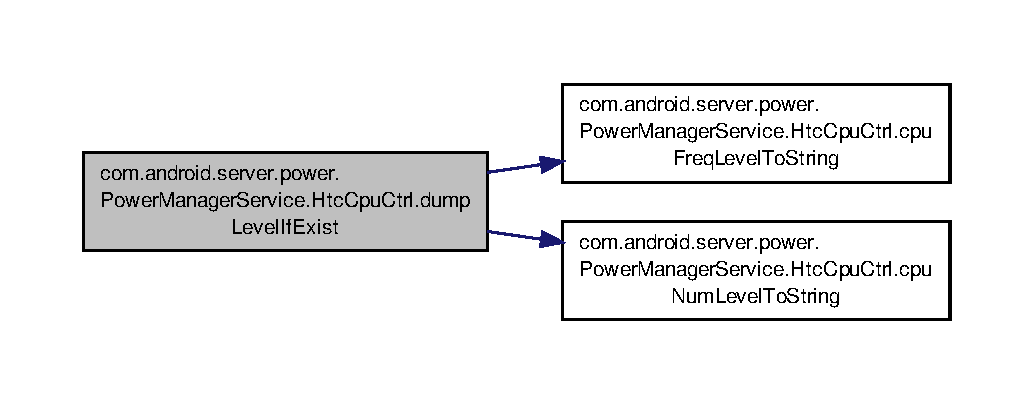
\includegraphics[width=350pt]{classcom_1_1android_1_1server_1_1power_1_1PowerManagerService_1_1HtcCpuCtrl_a095dd0137eb8fdb5155505205400d0c9_cgraph}
\end{center}
\end{figure}


\hypertarget{classcom_1_1android_1_1server_1_1power_1_1PowerManagerService_1_1HtcCpuCtrl_ada5ade08fc1bbc694eb3fbad8238102c}{\index{com\-::android\-::server\-::power\-::\-Power\-Manager\-Service\-::\-Htc\-Cpu\-Ctrl@{com\-::android\-::server\-::power\-::\-Power\-Manager\-Service\-::\-Htc\-Cpu\-Ctrl}!get\-Level@{get\-Level}}
\index{get\-Level@{get\-Level}!com::android::server::power::PowerManagerService::HtcCpuCtrl@{com\-::android\-::server\-::power\-::\-Power\-Manager\-Service\-::\-Htc\-Cpu\-Ctrl}}
\subsubsection[{get\-Level}]{\setlength{\rightskip}{0pt plus 5cm}int com.\-android.\-server.\-power.\-Power\-Manager\-Service.\-Htc\-Cpu\-Ctrl.\-get\-Level (
\begin{DoxyParamCaption}
{}
\end{DoxyParamCaption}
)\hspace{0.3cm}{\ttfamily [inline]}}}\label{classcom_1_1android_1_1server_1_1power_1_1PowerManagerService_1_1HtcCpuCtrl_ada5ade08fc1bbc694eb3fbad8238102c}
\hypertarget{classcom_1_1android_1_1server_1_1power_1_1PowerManagerService_1_1HtcCpuCtrl_a56baa8905bc9d8a055b65b8a4f86a4fc}{\index{com\-::android\-::server\-::power\-::\-Power\-Manager\-Service\-::\-Htc\-Cpu\-Ctrl@{com\-::android\-::server\-::power\-::\-Power\-Manager\-Service\-::\-Htc\-Cpu\-Ctrl}!get\-Lock\-Level\-String@{get\-Lock\-Level\-String}}
\index{get\-Lock\-Level\-String@{get\-Lock\-Level\-String}!com::android::server::power::PowerManagerService::HtcCpuCtrl@{com\-::android\-::server\-::power\-::\-Power\-Manager\-Service\-::\-Htc\-Cpu\-Ctrl}}
\subsubsection[{get\-Lock\-Level\-String}]{\setlength{\rightskip}{0pt plus 5cm}String com.\-android.\-server.\-power.\-Power\-Manager\-Service.\-Htc\-Cpu\-Ctrl.\-get\-Lock\-Level\-String (
\begin{DoxyParamCaption}
{}
\end{DoxyParamCaption}
)\hspace{0.3cm}{\ttfamily [inline]}, {\ttfamily [private]}}}\label{classcom_1_1android_1_1server_1_1power_1_1PowerManagerService_1_1HtcCpuCtrl_a56baa8905bc9d8a055b65b8a4f86a4fc}
\hypertarget{classcom_1_1android_1_1server_1_1power_1_1PowerManagerService_1_1HtcCpuCtrl_a7da367150c7c4506ceffbac3283ee7e9}{\index{com\-::android\-::server\-::power\-::\-Power\-Manager\-Service\-::\-Htc\-Cpu\-Ctrl@{com\-::android\-::server\-::power\-::\-Power\-Manager\-Service\-::\-Htc\-Cpu\-Ctrl}!has\-Same\-Properties@{has\-Same\-Properties}}
\index{has\-Same\-Properties@{has\-Same\-Properties}!com::android::server::power::PowerManagerService::HtcCpuCtrl@{com\-::android\-::server\-::power\-::\-Power\-Manager\-Service\-::\-Htc\-Cpu\-Ctrl}}
\subsubsection[{has\-Same\-Properties}]{\setlength{\rightskip}{0pt plus 5cm}boolean com.\-android.\-server.\-power.\-Power\-Manager\-Service.\-Htc\-Cpu\-Ctrl.\-has\-Same\-Properties (
\begin{DoxyParamCaption}
\item[{int}]{flags, }
\item[{String}]{tag, }
\item[{Work\-Source}]{work\-Source, }
\item[{int}]{owner\-Uid, }
\item[{int}]{owner\-Pid}
\end{DoxyParamCaption}
)\hspace{0.3cm}{\ttfamily [inline]}}}\label{classcom_1_1android_1_1server_1_1power_1_1PowerManagerService_1_1HtcCpuCtrl_a7da367150c7c4506ceffbac3283ee7e9}


Here is the call graph for this function\-:
\nopagebreak
\begin{figure}[H]
\begin{center}
\leavevmode
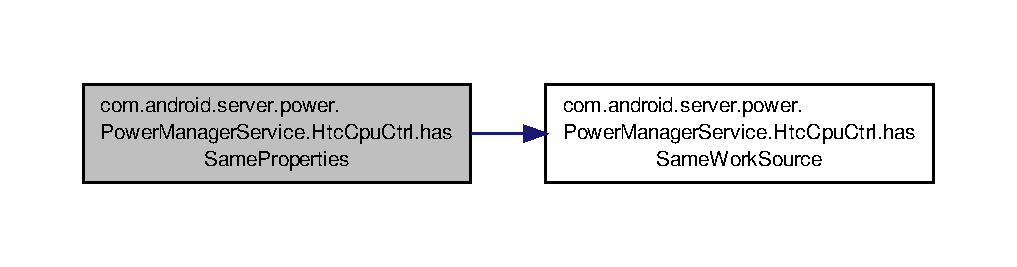
\includegraphics[width=350pt]{classcom_1_1android_1_1server_1_1power_1_1PowerManagerService_1_1HtcCpuCtrl_a7da367150c7c4506ceffbac3283ee7e9_cgraph}
\end{center}
\end{figure}


\hypertarget{classcom_1_1android_1_1server_1_1power_1_1PowerManagerService_1_1HtcCpuCtrl_a31b1cc24bd6f3624ad1a71eafe2fad64}{\index{com\-::android\-::server\-::power\-::\-Power\-Manager\-Service\-::\-Htc\-Cpu\-Ctrl@{com\-::android\-::server\-::power\-::\-Power\-Manager\-Service\-::\-Htc\-Cpu\-Ctrl}!has\-Same\-Work\-Source@{has\-Same\-Work\-Source}}
\index{has\-Same\-Work\-Source@{has\-Same\-Work\-Source}!com::android::server::power::PowerManagerService::HtcCpuCtrl@{com\-::android\-::server\-::power\-::\-Power\-Manager\-Service\-::\-Htc\-Cpu\-Ctrl}}
\subsubsection[{has\-Same\-Work\-Source}]{\setlength{\rightskip}{0pt plus 5cm}boolean com.\-android.\-server.\-power.\-Power\-Manager\-Service.\-Htc\-Cpu\-Ctrl.\-has\-Same\-Work\-Source (
\begin{DoxyParamCaption}
\item[{Work\-Source}]{work\-Source}
\end{DoxyParamCaption}
)\hspace{0.3cm}{\ttfamily [inline]}}}\label{classcom_1_1android_1_1server_1_1power_1_1PowerManagerService_1_1HtcCpuCtrl_a31b1cc24bd6f3624ad1a71eafe2fad64}
\hypertarget{classcom_1_1android_1_1server_1_1power_1_1PowerManagerService_1_1HtcCpuCtrl_a2e8197ca6777001ab61ab5ce23db7907}{\index{com\-::android\-::server\-::power\-::\-Power\-Manager\-Service\-::\-Htc\-Cpu\-Ctrl@{com\-::android\-::server\-::power\-::\-Power\-Manager\-Service\-::\-Htc\-Cpu\-Ctrl}!to\-String@{to\-String}}
\index{to\-String@{to\-String}!com::android::server::power::PowerManagerService::HtcCpuCtrl@{com\-::android\-::server\-::power\-::\-Power\-Manager\-Service\-::\-Htc\-Cpu\-Ctrl}}
\subsubsection[{to\-String}]{\setlength{\rightskip}{0pt plus 5cm}String com.\-android.\-server.\-power.\-Power\-Manager\-Service.\-Htc\-Cpu\-Ctrl.\-to\-String (
\begin{DoxyParamCaption}
{}
\end{DoxyParamCaption}
)\hspace{0.3cm}{\ttfamily [inline]}}}\label{classcom_1_1android_1_1server_1_1power_1_1PowerManagerService_1_1HtcCpuCtrl_a2e8197ca6777001ab61ab5ce23db7907}


Here is the call graph for this function\-:
\nopagebreak
\begin{figure}[H]
\begin{center}
\leavevmode
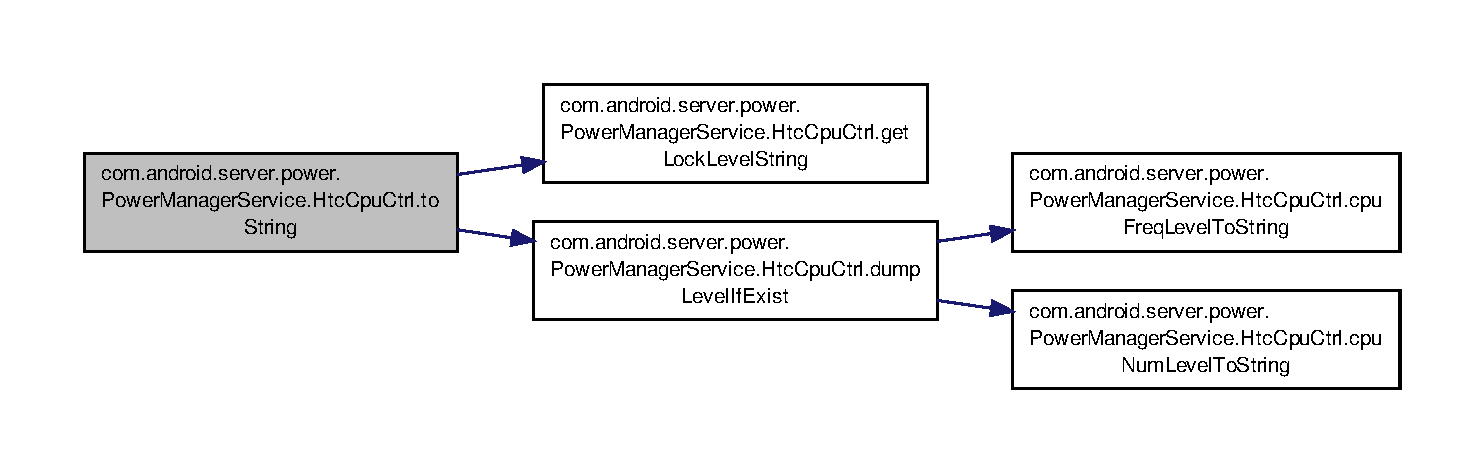
\includegraphics[width=350pt]{classcom_1_1android_1_1server_1_1power_1_1PowerManagerService_1_1HtcCpuCtrl_a2e8197ca6777001ab61ab5ce23db7907_cgraph}
\end{center}
\end{figure}


\hypertarget{classcom_1_1android_1_1server_1_1power_1_1PowerManagerService_1_1HtcCpuCtrl_a97aaf5d3af48928c73af170a64a869b3}{\index{com\-::android\-::server\-::power\-::\-Power\-Manager\-Service\-::\-Htc\-Cpu\-Ctrl@{com\-::android\-::server\-::power\-::\-Power\-Manager\-Service\-::\-Htc\-Cpu\-Ctrl}!update\-Properties@{update\-Properties}}
\index{update\-Properties@{update\-Properties}!com::android::server::power::PowerManagerService::HtcCpuCtrl@{com\-::android\-::server\-::power\-::\-Power\-Manager\-Service\-::\-Htc\-Cpu\-Ctrl}}
\subsubsection[{update\-Properties}]{\setlength{\rightskip}{0pt plus 5cm}void com.\-android.\-server.\-power.\-Power\-Manager\-Service.\-Htc\-Cpu\-Ctrl.\-update\-Properties (
\begin{DoxyParamCaption}
\item[{int}]{flags, }
\item[{String}]{tag, }
\item[{Work\-Source}]{work\-Source, }
\item[{int}]{owner\-Uid, }
\item[{int}]{owner\-Pid}
\end{DoxyParamCaption}
)\hspace{0.3cm}{\ttfamily [inline]}}}\label{classcom_1_1android_1_1server_1_1power_1_1PowerManagerService_1_1HtcCpuCtrl_a97aaf5d3af48928c73af170a64a869b3}


Here is the call graph for this function\-:
\nopagebreak
\begin{figure}[H]
\begin{center}
\leavevmode
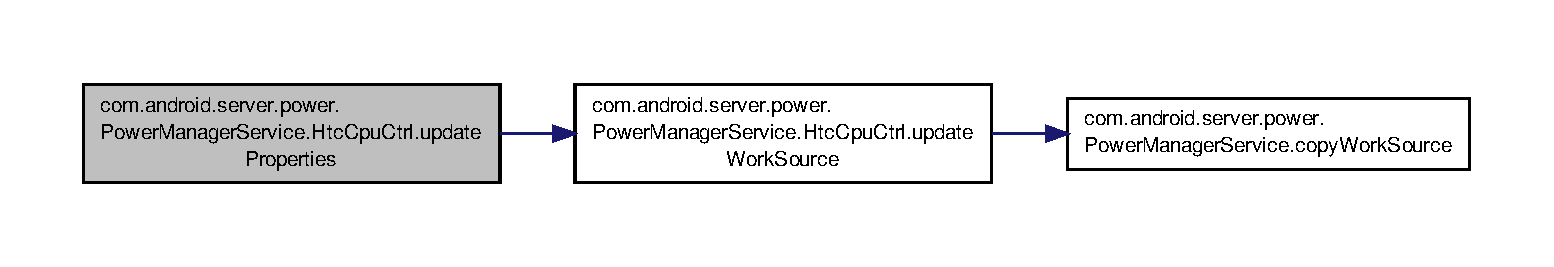
\includegraphics[width=350pt]{classcom_1_1android_1_1server_1_1power_1_1PowerManagerService_1_1HtcCpuCtrl_a97aaf5d3af48928c73af170a64a869b3_cgraph}
\end{center}
\end{figure}


\hypertarget{classcom_1_1android_1_1server_1_1power_1_1PowerManagerService_1_1HtcCpuCtrl_abd81472be2ab5e7eccc8c68840b3bbfa}{\index{com\-::android\-::server\-::power\-::\-Power\-Manager\-Service\-::\-Htc\-Cpu\-Ctrl@{com\-::android\-::server\-::power\-::\-Power\-Manager\-Service\-::\-Htc\-Cpu\-Ctrl}!update\-Work\-Source@{update\-Work\-Source}}
\index{update\-Work\-Source@{update\-Work\-Source}!com::android::server::power::PowerManagerService::HtcCpuCtrl@{com\-::android\-::server\-::power\-::\-Power\-Manager\-Service\-::\-Htc\-Cpu\-Ctrl}}
\subsubsection[{update\-Work\-Source}]{\setlength{\rightskip}{0pt plus 5cm}void com.\-android.\-server.\-power.\-Power\-Manager\-Service.\-Htc\-Cpu\-Ctrl.\-update\-Work\-Source (
\begin{DoxyParamCaption}
\item[{Work\-Source}]{work\-Source}
\end{DoxyParamCaption}
)\hspace{0.3cm}{\ttfamily [inline]}}}\label{classcom_1_1android_1_1server_1_1power_1_1PowerManagerService_1_1HtcCpuCtrl_abd81472be2ab5e7eccc8c68840b3bbfa}


Here is the call graph for this function\-:
\nopagebreak
\begin{figure}[H]
\begin{center}
\leavevmode
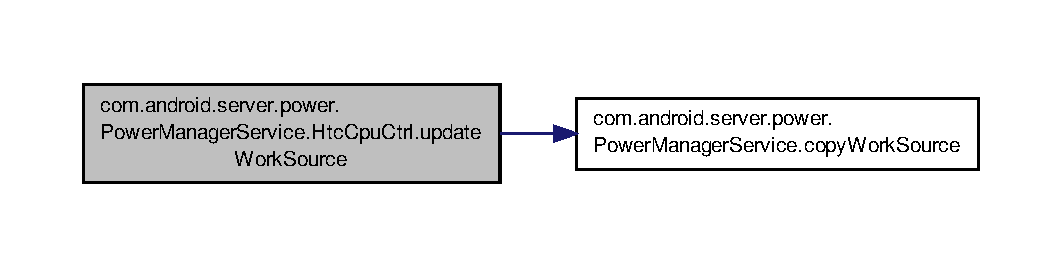
\includegraphics[width=350pt]{classcom_1_1android_1_1server_1_1power_1_1PowerManagerService_1_1HtcCpuCtrl_abd81472be2ab5e7eccc8c68840b3bbfa_cgraph}
\end{center}
\end{figure}




\subsection{Member Data Documentation}
\hypertarget{classcom_1_1android_1_1server_1_1power_1_1PowerManagerService_1_1HtcCpuCtrl_a9658c794544e425656117e195286043f}{\index{com\-::android\-::server\-::power\-::\-Power\-Manager\-Service\-::\-Htc\-Cpu\-Ctrl@{com\-::android\-::server\-::power\-::\-Power\-Manager\-Service\-::\-Htc\-Cpu\-Ctrl}!m\-Flags@{m\-Flags}}
\index{m\-Flags@{m\-Flags}!com::android::server::power::PowerManagerService::HtcCpuCtrl@{com\-::android\-::server\-::power\-::\-Power\-Manager\-Service\-::\-Htc\-Cpu\-Ctrl}}
\subsubsection[{m\-Flags}]{\setlength{\rightskip}{0pt plus 5cm}int com.\-android.\-server.\-power.\-Power\-Manager\-Service.\-Htc\-Cpu\-Ctrl.\-m\-Flags}}\label{classcom_1_1android_1_1server_1_1power_1_1PowerManagerService_1_1HtcCpuCtrl_a9658c794544e425656117e195286043f}
\hypertarget{classcom_1_1android_1_1server_1_1power_1_1PowerManagerService_1_1HtcCpuCtrl_a6a210dc8e827717053a51bf27c637e0b}{\index{com\-::android\-::server\-::power\-::\-Power\-Manager\-Service\-::\-Htc\-Cpu\-Ctrl@{com\-::android\-::server\-::power\-::\-Power\-Manager\-Service\-::\-Htc\-Cpu\-Ctrl}!m\-Level@{m\-Level}}
\index{m\-Level@{m\-Level}!com::android::server::power::PowerManagerService::HtcCpuCtrl@{com\-::android\-::server\-::power\-::\-Power\-Manager\-Service\-::\-Htc\-Cpu\-Ctrl}}
\subsubsection[{m\-Level}]{\setlength{\rightskip}{0pt plus 5cm}int com.\-android.\-server.\-power.\-Power\-Manager\-Service.\-Htc\-Cpu\-Ctrl.\-m\-Level\hspace{0.3cm}{\ttfamily [private]}}}\label{classcom_1_1android_1_1server_1_1power_1_1PowerManagerService_1_1HtcCpuCtrl_a6a210dc8e827717053a51bf27c637e0b}
\hypertarget{classcom_1_1android_1_1server_1_1power_1_1PowerManagerService_1_1HtcCpuCtrl_a9c26de2babb8433dad620487e6da90ee}{\index{com\-::android\-::server\-::power\-::\-Power\-Manager\-Service\-::\-Htc\-Cpu\-Ctrl@{com\-::android\-::server\-::power\-::\-Power\-Manager\-Service\-::\-Htc\-Cpu\-Ctrl}!m\-Lock@{m\-Lock}}
\index{m\-Lock@{m\-Lock}!com::android::server::power::PowerManagerService::HtcCpuCtrl@{com\-::android\-::server\-::power\-::\-Power\-Manager\-Service\-::\-Htc\-Cpu\-Ctrl}}
\subsubsection[{m\-Lock}]{\setlength{\rightskip}{0pt plus 5cm}final I\-Binder com.\-android.\-server.\-power.\-Power\-Manager\-Service.\-Htc\-Cpu\-Ctrl.\-m\-Lock}}\label{classcom_1_1android_1_1server_1_1power_1_1PowerManagerService_1_1HtcCpuCtrl_a9c26de2babb8433dad620487e6da90ee}
\hypertarget{classcom_1_1android_1_1server_1_1power_1_1PowerManagerService_1_1HtcCpuCtrl_adf0bb931ec82c6a5b68d8b2ab0c451b1}{\index{com\-::android\-::server\-::power\-::\-Power\-Manager\-Service\-::\-Htc\-Cpu\-Ctrl@{com\-::android\-::server\-::power\-::\-Power\-Manager\-Service\-::\-Htc\-Cpu\-Ctrl}!m\-Owner\-Pid@{m\-Owner\-Pid}}
\index{m\-Owner\-Pid@{m\-Owner\-Pid}!com::android::server::power::PowerManagerService::HtcCpuCtrl@{com\-::android\-::server\-::power\-::\-Power\-Manager\-Service\-::\-Htc\-Cpu\-Ctrl}}
\subsubsection[{m\-Owner\-Pid}]{\setlength{\rightskip}{0pt plus 5cm}int com.\-android.\-server.\-power.\-Power\-Manager\-Service.\-Htc\-Cpu\-Ctrl.\-m\-Owner\-Pid}}\label{classcom_1_1android_1_1server_1_1power_1_1PowerManagerService_1_1HtcCpuCtrl_adf0bb931ec82c6a5b68d8b2ab0c451b1}
\hypertarget{classcom_1_1android_1_1server_1_1power_1_1PowerManagerService_1_1HtcCpuCtrl_ac14893ba75fd5aa8d1d1c7173adb90a0}{\index{com\-::android\-::server\-::power\-::\-Power\-Manager\-Service\-::\-Htc\-Cpu\-Ctrl@{com\-::android\-::server\-::power\-::\-Power\-Manager\-Service\-::\-Htc\-Cpu\-Ctrl}!m\-Owner\-Uid@{m\-Owner\-Uid}}
\index{m\-Owner\-Uid@{m\-Owner\-Uid}!com::android::server::power::PowerManagerService::HtcCpuCtrl@{com\-::android\-::server\-::power\-::\-Power\-Manager\-Service\-::\-Htc\-Cpu\-Ctrl}}
\subsubsection[{m\-Owner\-Uid}]{\setlength{\rightskip}{0pt plus 5cm}int com.\-android.\-server.\-power.\-Power\-Manager\-Service.\-Htc\-Cpu\-Ctrl.\-m\-Owner\-Uid}}\label{classcom_1_1android_1_1server_1_1power_1_1PowerManagerService_1_1HtcCpuCtrl_ac14893ba75fd5aa8d1d1c7173adb90a0}
\hypertarget{classcom_1_1android_1_1server_1_1power_1_1PowerManagerService_1_1HtcCpuCtrl_acd2763c41cf2375b632557850fa9f0cd}{\index{com\-::android\-::server\-::power\-::\-Power\-Manager\-Service\-::\-Htc\-Cpu\-Ctrl@{com\-::android\-::server\-::power\-::\-Power\-Manager\-Service\-::\-Htc\-Cpu\-Ctrl}!m\-Tag@{m\-Tag}}
\index{m\-Tag@{m\-Tag}!com::android::server::power::PowerManagerService::HtcCpuCtrl@{com\-::android\-::server\-::power\-::\-Power\-Manager\-Service\-::\-Htc\-Cpu\-Ctrl}}
\subsubsection[{m\-Tag}]{\setlength{\rightskip}{0pt plus 5cm}String com.\-android.\-server.\-power.\-Power\-Manager\-Service.\-Htc\-Cpu\-Ctrl.\-m\-Tag}}\label{classcom_1_1android_1_1server_1_1power_1_1PowerManagerService_1_1HtcCpuCtrl_acd2763c41cf2375b632557850fa9f0cd}
\hypertarget{classcom_1_1android_1_1server_1_1power_1_1PowerManagerService_1_1HtcCpuCtrl_a29942ea13180d98f1a9e4ea444834d1b}{\index{com\-::android\-::server\-::power\-::\-Power\-Manager\-Service\-::\-Htc\-Cpu\-Ctrl@{com\-::android\-::server\-::power\-::\-Power\-Manager\-Service\-::\-Htc\-Cpu\-Ctrl}!m\-Work\-Source@{m\-Work\-Source}}
\index{m\-Work\-Source@{m\-Work\-Source}!com::android::server::power::PowerManagerService::HtcCpuCtrl@{com\-::android\-::server\-::power\-::\-Power\-Manager\-Service\-::\-Htc\-Cpu\-Ctrl}}
\subsubsection[{m\-Work\-Source}]{\setlength{\rightskip}{0pt plus 5cm}Work\-Source com.\-android.\-server.\-power.\-Power\-Manager\-Service.\-Htc\-Cpu\-Ctrl.\-m\-Work\-Source}}\label{classcom_1_1android_1_1server_1_1power_1_1PowerManagerService_1_1HtcCpuCtrl_a29942ea13180d98f1a9e4ea444834d1b}


The documentation for this class was generated from the following file\-:\begin{DoxyCompactItemize}
\item 
\hyperlink{PowerManagerService_8java}{Power\-Manager\-Service.\-java}\end{DoxyCompactItemize}

\hypertarget{classcom_1_1android_1_1server_1_1power_1_1ElectronBeam_1_1NaturalSurfaceLayout}{\section{com.\-android.\-server.\-power.\-Electron\-Beam.\-Natural\-Surface\-Layout Class Reference}
\label{classcom_1_1android_1_1server_1_1power_1_1ElectronBeam_1_1NaturalSurfaceLayout}\index{com.\-android.\-server.\-power.\-Electron\-Beam.\-Natural\-Surface\-Layout@{com.\-android.\-server.\-power.\-Electron\-Beam.\-Natural\-Surface\-Layout}}
}


Inheritance diagram for com.\-android.\-server.\-power.\-Electron\-Beam.\-Natural\-Surface\-Layout\-:
\nopagebreak
\begin{figure}[H]
\begin{center}
\leavevmode
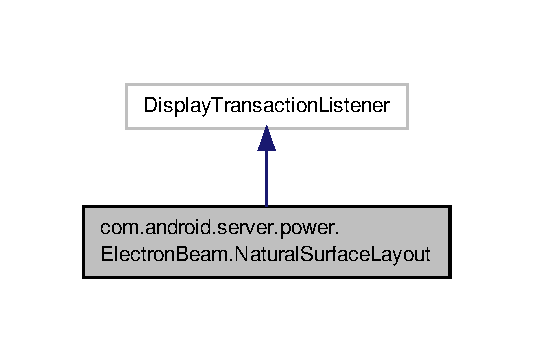
\includegraphics[width=256pt]{classcom_1_1android_1_1server_1_1power_1_1ElectronBeam_1_1NaturalSurfaceLayout__inherit__graph}
\end{center}
\end{figure}


Collaboration diagram for com.\-android.\-server.\-power.\-Electron\-Beam.\-Natural\-Surface\-Layout\-:
\nopagebreak
\begin{figure}[H]
\begin{center}
\leavevmode
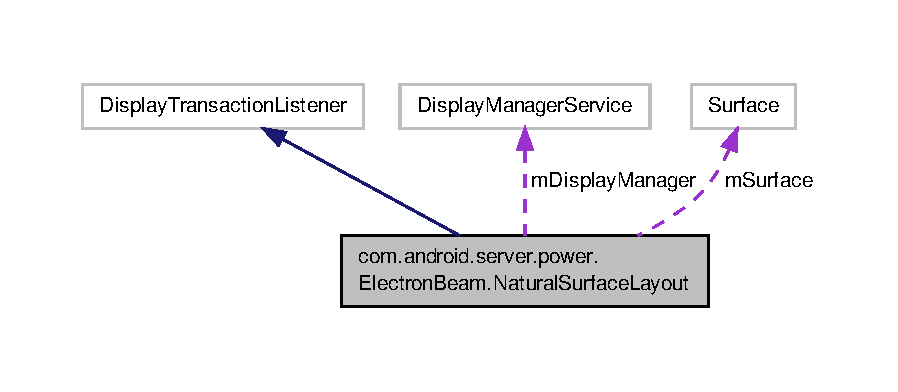
\includegraphics[width=350pt]{classcom_1_1android_1_1server_1_1power_1_1ElectronBeam_1_1NaturalSurfaceLayout__coll__graph}
\end{center}
\end{figure}
\subsection*{Public Member Functions}
\begin{DoxyCompactItemize}
\item 
\hyperlink{classcom_1_1android_1_1server_1_1power_1_1ElectronBeam_1_1NaturalSurfaceLayout_a36c9443f02e9afb0e21ac248aec3c04d}{Natural\-Surface\-Layout} (Display\-Manager\-Service display\-Manager, Surface surface)
\item 
void \hyperlink{classcom_1_1android_1_1server_1_1power_1_1ElectronBeam_1_1NaturalSurfaceLayout_a42e7b039790c30ea68acdb8df6bd95a5}{dispose} ()
\item 
void \hyperlink{classcom_1_1android_1_1server_1_1power_1_1ElectronBeam_1_1NaturalSurfaceLayout_a4de66347d52f912fb7878aac9f0c0887}{on\-Display\-Transaction} ()
\end{DoxyCompactItemize}
\subsection*{Private Attributes}
\begin{DoxyCompactItemize}
\item 
final Display\-Manager\-Service \hyperlink{classcom_1_1android_1_1server_1_1power_1_1ElectronBeam_1_1NaturalSurfaceLayout_a5b437ab809caf97d241478ce52c6c932}{m\-Display\-Manager}
\item 
Surface \hyperlink{classcom_1_1android_1_1server_1_1power_1_1ElectronBeam_1_1NaturalSurfaceLayout_abb69c08305d023474da59b30206b8fd8}{m\-Surface}
\end{DoxyCompactItemize}


\subsection{Detailed Description}
Keeps a surface aligned with the natural orientation of the device. Updates the position and transformation of the matrix whenever the display is rotated. This is a little tricky because the display transaction callback can be invoked on any thread, not necessarily the thread that owns the electron beam. 

\subsection{Constructor \& Destructor Documentation}
\hypertarget{classcom_1_1android_1_1server_1_1power_1_1ElectronBeam_1_1NaturalSurfaceLayout_a36c9443f02e9afb0e21ac248aec3c04d}{\index{com\-::android\-::server\-::power\-::\-Electron\-Beam\-::\-Natural\-Surface\-Layout@{com\-::android\-::server\-::power\-::\-Electron\-Beam\-::\-Natural\-Surface\-Layout}!Natural\-Surface\-Layout@{Natural\-Surface\-Layout}}
\index{Natural\-Surface\-Layout@{Natural\-Surface\-Layout}!com::android::server::power::ElectronBeam::NaturalSurfaceLayout@{com\-::android\-::server\-::power\-::\-Electron\-Beam\-::\-Natural\-Surface\-Layout}}
\subsubsection[{Natural\-Surface\-Layout}]{\setlength{\rightskip}{0pt plus 5cm}com.\-android.\-server.\-power.\-Electron\-Beam.\-Natural\-Surface\-Layout.\-Natural\-Surface\-Layout (
\begin{DoxyParamCaption}
\item[{Display\-Manager\-Service}]{display\-Manager, }
\item[{Surface}]{surface}
\end{DoxyParamCaption}
)\hspace{0.3cm}{\ttfamily [inline]}}}\label{classcom_1_1android_1_1server_1_1power_1_1ElectronBeam_1_1NaturalSurfaceLayout_a36c9443f02e9afb0e21ac248aec3c04d}


\subsection{Member Function Documentation}
\hypertarget{classcom_1_1android_1_1server_1_1power_1_1ElectronBeam_1_1NaturalSurfaceLayout_a42e7b039790c30ea68acdb8df6bd95a5}{\index{com\-::android\-::server\-::power\-::\-Electron\-Beam\-::\-Natural\-Surface\-Layout@{com\-::android\-::server\-::power\-::\-Electron\-Beam\-::\-Natural\-Surface\-Layout}!dispose@{dispose}}
\index{dispose@{dispose}!com::android::server::power::ElectronBeam::NaturalSurfaceLayout@{com\-::android\-::server\-::power\-::\-Electron\-Beam\-::\-Natural\-Surface\-Layout}}
\subsubsection[{dispose}]{\setlength{\rightskip}{0pt plus 5cm}void com.\-android.\-server.\-power.\-Electron\-Beam.\-Natural\-Surface\-Layout.\-dispose (
\begin{DoxyParamCaption}
{}
\end{DoxyParamCaption}
)\hspace{0.3cm}{\ttfamily [inline]}}}\label{classcom_1_1android_1_1server_1_1power_1_1ElectronBeam_1_1NaturalSurfaceLayout_a42e7b039790c30ea68acdb8df6bd95a5}
\hypertarget{classcom_1_1android_1_1server_1_1power_1_1ElectronBeam_1_1NaturalSurfaceLayout_a4de66347d52f912fb7878aac9f0c0887}{\index{com\-::android\-::server\-::power\-::\-Electron\-Beam\-::\-Natural\-Surface\-Layout@{com\-::android\-::server\-::power\-::\-Electron\-Beam\-::\-Natural\-Surface\-Layout}!on\-Display\-Transaction@{on\-Display\-Transaction}}
\index{on\-Display\-Transaction@{on\-Display\-Transaction}!com::android::server::power::ElectronBeam::NaturalSurfaceLayout@{com\-::android\-::server\-::power\-::\-Electron\-Beam\-::\-Natural\-Surface\-Layout}}
\subsubsection[{on\-Display\-Transaction}]{\setlength{\rightskip}{0pt plus 5cm}void com.\-android.\-server.\-power.\-Electron\-Beam.\-Natural\-Surface\-Layout.\-on\-Display\-Transaction (
\begin{DoxyParamCaption}
{}
\end{DoxyParamCaption}
)\hspace{0.3cm}{\ttfamily [inline]}}}\label{classcom_1_1android_1_1server_1_1power_1_1ElectronBeam_1_1NaturalSurfaceLayout_a4de66347d52f912fb7878aac9f0c0887}


\subsection{Member Data Documentation}
\hypertarget{classcom_1_1android_1_1server_1_1power_1_1ElectronBeam_1_1NaturalSurfaceLayout_a5b437ab809caf97d241478ce52c6c932}{\index{com\-::android\-::server\-::power\-::\-Electron\-Beam\-::\-Natural\-Surface\-Layout@{com\-::android\-::server\-::power\-::\-Electron\-Beam\-::\-Natural\-Surface\-Layout}!m\-Display\-Manager@{m\-Display\-Manager}}
\index{m\-Display\-Manager@{m\-Display\-Manager}!com::android::server::power::ElectronBeam::NaturalSurfaceLayout@{com\-::android\-::server\-::power\-::\-Electron\-Beam\-::\-Natural\-Surface\-Layout}}
\subsubsection[{m\-Display\-Manager}]{\setlength{\rightskip}{0pt plus 5cm}final Display\-Manager\-Service com.\-android.\-server.\-power.\-Electron\-Beam.\-Natural\-Surface\-Layout.\-m\-Display\-Manager\hspace{0.3cm}{\ttfamily [private]}}}\label{classcom_1_1android_1_1server_1_1power_1_1ElectronBeam_1_1NaturalSurfaceLayout_a5b437ab809caf97d241478ce52c6c932}
\hypertarget{classcom_1_1android_1_1server_1_1power_1_1ElectronBeam_1_1NaturalSurfaceLayout_abb69c08305d023474da59b30206b8fd8}{\index{com\-::android\-::server\-::power\-::\-Electron\-Beam\-::\-Natural\-Surface\-Layout@{com\-::android\-::server\-::power\-::\-Electron\-Beam\-::\-Natural\-Surface\-Layout}!m\-Surface@{m\-Surface}}
\index{m\-Surface@{m\-Surface}!com::android::server::power::ElectronBeam::NaturalSurfaceLayout@{com\-::android\-::server\-::power\-::\-Electron\-Beam\-::\-Natural\-Surface\-Layout}}
\subsubsection[{m\-Surface}]{\setlength{\rightskip}{0pt plus 5cm}Surface com.\-android.\-server.\-power.\-Electron\-Beam.\-Natural\-Surface\-Layout.\-m\-Surface\hspace{0.3cm}{\ttfamily [private]}}}\label{classcom_1_1android_1_1server_1_1power_1_1ElectronBeam_1_1NaturalSurfaceLayout_abb69c08305d023474da59b30206b8fd8}


The documentation for this class was generated from the following file\-:\begin{DoxyCompactItemize}
\item 
\hyperlink{ElectronBeam_8java}{Electron\-Beam.\-java}\end{DoxyCompactItemize}

\hypertarget{classcom_1_1android_1_1server_1_1power_1_1Notifier_1_1NotifierHandler}{\section{com.\-android.\-server.\-power.\-Notifier.\-Notifier\-Handler Class Reference}
\label{classcom_1_1android_1_1server_1_1power_1_1Notifier_1_1NotifierHandler}\index{com.\-android.\-server.\-power.\-Notifier.\-Notifier\-Handler@{com.\-android.\-server.\-power.\-Notifier.\-Notifier\-Handler}}
}


Inheritance diagram for com.\-android.\-server.\-power.\-Notifier.\-Notifier\-Handler\-:
\nopagebreak
\begin{figure}[H]
\begin{center}
\leavevmode
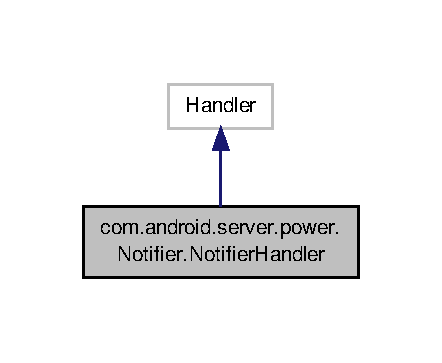
\includegraphics[width=212pt]{classcom_1_1android_1_1server_1_1power_1_1Notifier_1_1NotifierHandler__inherit__graph}
\end{center}
\end{figure}


Collaboration diagram for com.\-android.\-server.\-power.\-Notifier.\-Notifier\-Handler\-:
\nopagebreak
\begin{figure}[H]
\begin{center}
\leavevmode
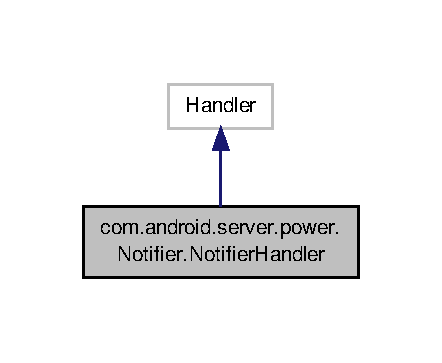
\includegraphics[width=212pt]{classcom_1_1android_1_1server_1_1power_1_1Notifier_1_1NotifierHandler__coll__graph}
\end{center}
\end{figure}
\subsection*{Public Member Functions}
\begin{DoxyCompactItemize}
\item 
\hyperlink{classcom_1_1android_1_1server_1_1power_1_1Notifier_1_1NotifierHandler_a41deb23331f45ee19d9f4b6602d9c408}{Notifier\-Handler} (Looper looper)
\item 
void \hyperlink{classcom_1_1android_1_1server_1_1power_1_1Notifier_1_1NotifierHandler_a3ab4d794ca3a712b7107fe67709e3eb6}{handle\-Message} (Message msg)
\end{DoxyCompactItemize}


\subsection{Constructor \& Destructor Documentation}
\hypertarget{classcom_1_1android_1_1server_1_1power_1_1Notifier_1_1NotifierHandler_a41deb23331f45ee19d9f4b6602d9c408}{\index{com\-::android\-::server\-::power\-::\-Notifier\-::\-Notifier\-Handler@{com\-::android\-::server\-::power\-::\-Notifier\-::\-Notifier\-Handler}!Notifier\-Handler@{Notifier\-Handler}}
\index{Notifier\-Handler@{Notifier\-Handler}!com::android::server::power::Notifier::NotifierHandler@{com\-::android\-::server\-::power\-::\-Notifier\-::\-Notifier\-Handler}}
\subsubsection[{Notifier\-Handler}]{\setlength{\rightskip}{0pt plus 5cm}com.\-android.\-server.\-power.\-Notifier.\-Notifier\-Handler.\-Notifier\-Handler (
\begin{DoxyParamCaption}
\item[{Looper}]{looper}
\end{DoxyParamCaption}
)\hspace{0.3cm}{\ttfamily [inline]}}}\label{classcom_1_1android_1_1server_1_1power_1_1Notifier_1_1NotifierHandler_a41deb23331f45ee19d9f4b6602d9c408}


\subsection{Member Function Documentation}
\hypertarget{classcom_1_1android_1_1server_1_1power_1_1Notifier_1_1NotifierHandler_a3ab4d794ca3a712b7107fe67709e3eb6}{\index{com\-::android\-::server\-::power\-::\-Notifier\-::\-Notifier\-Handler@{com\-::android\-::server\-::power\-::\-Notifier\-::\-Notifier\-Handler}!handle\-Message@{handle\-Message}}
\index{handle\-Message@{handle\-Message}!com::android::server::power::Notifier::NotifierHandler@{com\-::android\-::server\-::power\-::\-Notifier\-::\-Notifier\-Handler}}
\subsubsection[{handle\-Message}]{\setlength{\rightskip}{0pt plus 5cm}void com.\-android.\-server.\-power.\-Notifier.\-Notifier\-Handler.\-handle\-Message (
\begin{DoxyParamCaption}
\item[{Message}]{msg}
\end{DoxyParamCaption}
)\hspace{0.3cm}{\ttfamily [inline]}}}\label{classcom_1_1android_1_1server_1_1power_1_1Notifier_1_1NotifierHandler_a3ab4d794ca3a712b7107fe67709e3eb6}


The documentation for this class was generated from the following file\-:\begin{DoxyCompactItemize}
\item 
\hyperlink{Notifier_8java}{Notifier.\-java}\end{DoxyCompactItemize}

\hypertarget{classcom_1_1android_1_1server_1_1power_1_1PowerManagerService_1_1OOBETimeoutReceiver}{\section{com.\-android.\-server.\-power.\-Power\-Manager\-Service.\-O\-O\-B\-E\-Timeout\-Receiver Class Reference}
\label{classcom_1_1android_1_1server_1_1power_1_1PowerManagerService_1_1OOBETimeoutReceiver}\index{com.\-android.\-server.\-power.\-Power\-Manager\-Service.\-O\-O\-B\-E\-Timeout\-Receiver@{com.\-android.\-server.\-power.\-Power\-Manager\-Service.\-O\-O\-B\-E\-Timeout\-Receiver}}
}


Inheritance diagram for com.\-android.\-server.\-power.\-Power\-Manager\-Service.\-O\-O\-B\-E\-Timeout\-Receiver\-:
\nopagebreak
\begin{figure}[H]
\begin{center}
\leavevmode
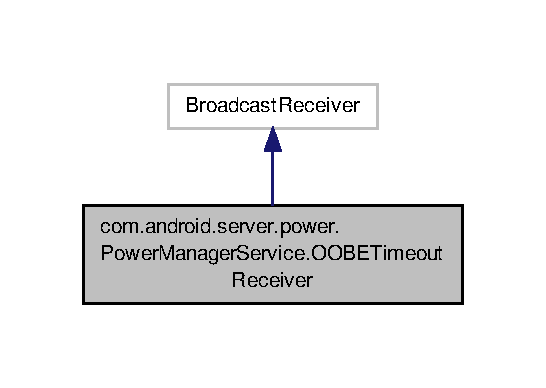
\includegraphics[width=262pt]{classcom_1_1android_1_1server_1_1power_1_1PowerManagerService_1_1OOBETimeoutReceiver__inherit__graph}
\end{center}
\end{figure}


Collaboration diagram for com.\-android.\-server.\-power.\-Power\-Manager\-Service.\-O\-O\-B\-E\-Timeout\-Receiver\-:
\nopagebreak
\begin{figure}[H]
\begin{center}
\leavevmode
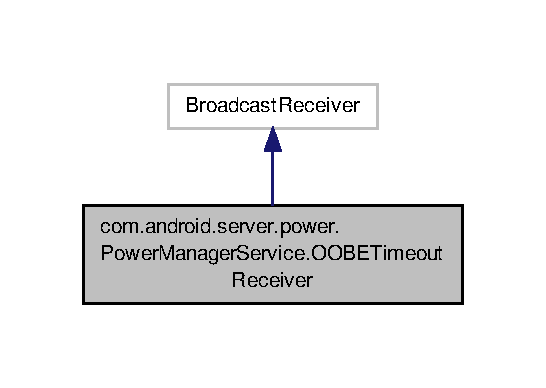
\includegraphics[width=262pt]{classcom_1_1android_1_1server_1_1power_1_1PowerManagerService_1_1OOBETimeoutReceiver__coll__graph}
\end{center}
\end{figure}
\subsection*{Public Member Functions}
\begin{DoxyCompactItemize}
\item 
void \hyperlink{classcom_1_1android_1_1server_1_1power_1_1PowerManagerService_1_1OOBETimeoutReceiver_abcc39669ac45306c8720cf578c488a8e}{on\-Receive} (Context context, Intent intent)
\end{DoxyCompactItemize}


\subsection{Member Function Documentation}
\hypertarget{classcom_1_1android_1_1server_1_1power_1_1PowerManagerService_1_1OOBETimeoutReceiver_abcc39669ac45306c8720cf578c488a8e}{\index{com\-::android\-::server\-::power\-::\-Power\-Manager\-Service\-::\-O\-O\-B\-E\-Timeout\-Receiver@{com\-::android\-::server\-::power\-::\-Power\-Manager\-Service\-::\-O\-O\-B\-E\-Timeout\-Receiver}!on\-Receive@{on\-Receive}}
\index{on\-Receive@{on\-Receive}!com::android::server::power::PowerManagerService::OOBETimeoutReceiver@{com\-::android\-::server\-::power\-::\-Power\-Manager\-Service\-::\-O\-O\-B\-E\-Timeout\-Receiver}}
\subsubsection[{on\-Receive}]{\setlength{\rightskip}{0pt plus 5cm}void com.\-android.\-server.\-power.\-Power\-Manager\-Service.\-O\-O\-B\-E\-Timeout\-Receiver.\-on\-Receive (
\begin{DoxyParamCaption}
\item[{Context}]{context, }
\item[{Intent}]{intent}
\end{DoxyParamCaption}
)\hspace{0.3cm}{\ttfamily [inline]}}}\label{classcom_1_1android_1_1server_1_1power_1_1PowerManagerService_1_1OOBETimeoutReceiver_abcc39669ac45306c8720cf578c488a8e}


The documentation for this class was generated from the following file\-:\begin{DoxyCompactItemize}
\item 
\hyperlink{PowerManagerService_8java}{Power\-Manager\-Service.\-java}\end{DoxyCompactItemize}

\hypertarget{classcom_1_1android_1_1server_1_1power_1_1DisplayPowerState_1_1PhotonicModulator}{\section{com.\-android.\-server.\-power.\-Display\-Power\-State.\-Photonic\-Modulator Class Reference}
\label{classcom_1_1android_1_1server_1_1power_1_1DisplayPowerState_1_1PhotonicModulator}\index{com.\-android.\-server.\-power.\-Display\-Power\-State.\-Photonic\-Modulator@{com.\-android.\-server.\-power.\-Display\-Power\-State.\-Photonic\-Modulator}}
}
\subsection*{Public Member Functions}
\begin{DoxyCompactItemize}
\item 
boolean \hyperlink{classcom_1_1android_1_1server_1_1power_1_1DisplayPowerState_1_1PhotonicModulator_a89a57d2602393b050bea05809ad00544}{set\-State} (boolean on, int backlight)
\item 
void \hyperlink{classcom_1_1android_1_1server_1_1power_1_1DisplayPowerState_1_1PhotonicModulator_a1985eb59872e7334f832b2762c8c07d7}{dump} (Print\-Writer pw)
\end{DoxyCompactItemize}
\subsection*{Private Attributes}
\begin{DoxyCompactItemize}
\item 
final Object \hyperlink{classcom_1_1android_1_1server_1_1power_1_1DisplayPowerState_1_1PhotonicModulator_a7be03ac416924266902cd7e001eb7044}{m\-Lock} = new Object()
\item 
boolean \hyperlink{classcom_1_1android_1_1server_1_1power_1_1DisplayPowerState_1_1PhotonicModulator_a5a7f23332c6937ca135a564157892816}{m\-Pending\-On} = \hyperlink{classcom_1_1android_1_1server_1_1power_1_1DisplayPowerState_1_1PhotonicModulator_aba2a7ba030813ba22a618a61511bfd48}{I\-N\-I\-T\-I\-A\-L\-\_\-\-S\-C\-R\-E\-E\-N\-\_\-\-O\-N}
\item 
int \hyperlink{classcom_1_1android_1_1server_1_1power_1_1DisplayPowerState_1_1PhotonicModulator_a382abc794aafa7743f1c2cff16f6a4ab}{m\-Pending\-Backlight} = \hyperlink{classcom_1_1android_1_1server_1_1power_1_1DisplayPowerState_1_1PhotonicModulator_ad07cac64078210d3346fea0041c25cfd}{I\-N\-I\-T\-I\-A\-L\-\_\-\-B\-A\-C\-K\-L\-I\-G\-H\-T}
\item 
boolean \hyperlink{classcom_1_1android_1_1server_1_1power_1_1DisplayPowerState_1_1PhotonicModulator_a9d38be17b604c637bc9430f55e2f4ba0}{m\-Actual\-On} = \hyperlink{classcom_1_1android_1_1server_1_1power_1_1DisplayPowerState_1_1PhotonicModulator_aba2a7ba030813ba22a618a61511bfd48}{I\-N\-I\-T\-I\-A\-L\-\_\-\-S\-C\-R\-E\-E\-N\-\_\-\-O\-N}
\item 
int \hyperlink{classcom_1_1android_1_1server_1_1power_1_1DisplayPowerState_1_1PhotonicModulator_a5e7e40b503507bedbc7808a473ce48f0}{m\-Actual\-Backlight} = \hyperlink{classcom_1_1android_1_1server_1_1power_1_1DisplayPowerState_1_1PhotonicModulator_ad07cac64078210d3346fea0041c25cfd}{I\-N\-I\-T\-I\-A\-L\-\_\-\-B\-A\-C\-K\-L\-I\-G\-H\-T}
\item 
boolean \hyperlink{classcom_1_1android_1_1server_1_1power_1_1DisplayPowerState_1_1PhotonicModulator_a76910dedf1065b2880753feecd8c3a09}{m\-Change\-In\-Progress}
\item 
int \hyperlink{classcom_1_1android_1_1server_1_1power_1_1DisplayPowerState_1_1PhotonicModulator_a0705a954e9dc796e3db0e162ed4b46ca}{m\-Current\-Button\-Value} = \hyperlink{classcom_1_1android_1_1server_1_1power_1_1DisplayPowerState_1_1PhotonicModulator_ad07cac64078210d3346fea0041c25cfd}{I\-N\-I\-T\-I\-A\-L\-\_\-\-B\-A\-C\-K\-L\-I\-G\-H\-T}
\item 
final Runnable \hyperlink{classcom_1_1android_1_1server_1_1power_1_1DisplayPowerState_1_1PhotonicModulator_af6dd80943227de9a16937b8d8b6f1ad4}{m\-Task}
\end{DoxyCompactItemize}
\subsection*{Static Private Attributes}
\begin{DoxyCompactItemize}
\item 
static final boolean \hyperlink{classcom_1_1android_1_1server_1_1power_1_1DisplayPowerState_1_1PhotonicModulator_aba2a7ba030813ba22a618a61511bfd48}{I\-N\-I\-T\-I\-A\-L\-\_\-\-S\-C\-R\-E\-E\-N\-\_\-\-O\-N} = false
\item 
static final int \hyperlink{classcom_1_1android_1_1server_1_1power_1_1DisplayPowerState_1_1PhotonicModulator_ad07cac64078210d3346fea0041c25cfd}{I\-N\-I\-T\-I\-A\-L\-\_\-\-B\-A\-C\-K\-L\-I\-G\-H\-T} = -\/1
\end{DoxyCompactItemize}


\subsection{Detailed Description}
Updates the state of the screen and backlight asynchronously on a separate thread. 

\subsection{Member Function Documentation}
\hypertarget{classcom_1_1android_1_1server_1_1power_1_1DisplayPowerState_1_1PhotonicModulator_a1985eb59872e7334f832b2762c8c07d7}{\index{com\-::android\-::server\-::power\-::\-Display\-Power\-State\-::\-Photonic\-Modulator@{com\-::android\-::server\-::power\-::\-Display\-Power\-State\-::\-Photonic\-Modulator}!dump@{dump}}
\index{dump@{dump}!com::android::server::power::DisplayPowerState::PhotonicModulator@{com\-::android\-::server\-::power\-::\-Display\-Power\-State\-::\-Photonic\-Modulator}}
\subsubsection[{dump}]{\setlength{\rightskip}{0pt plus 5cm}void com.\-android.\-server.\-power.\-Display\-Power\-State.\-Photonic\-Modulator.\-dump (
\begin{DoxyParamCaption}
\item[{Print\-Writer}]{pw}
\end{DoxyParamCaption}
)\hspace{0.3cm}{\ttfamily [inline]}}}\label{classcom_1_1android_1_1server_1_1power_1_1DisplayPowerState_1_1PhotonicModulator_a1985eb59872e7334f832b2762c8c07d7}
\hypertarget{classcom_1_1android_1_1server_1_1power_1_1DisplayPowerState_1_1PhotonicModulator_a89a57d2602393b050bea05809ad00544}{\index{com\-::android\-::server\-::power\-::\-Display\-Power\-State\-::\-Photonic\-Modulator@{com\-::android\-::server\-::power\-::\-Display\-Power\-State\-::\-Photonic\-Modulator}!set\-State@{set\-State}}
\index{set\-State@{set\-State}!com::android::server::power::DisplayPowerState::PhotonicModulator@{com\-::android\-::server\-::power\-::\-Display\-Power\-State\-::\-Photonic\-Modulator}}
\subsubsection[{set\-State}]{\setlength{\rightskip}{0pt plus 5cm}boolean com.\-android.\-server.\-power.\-Display\-Power\-State.\-Photonic\-Modulator.\-set\-State (
\begin{DoxyParamCaption}
\item[{boolean}]{on, }
\item[{int}]{backlight}
\end{DoxyParamCaption}
)\hspace{0.3cm}{\ttfamily [inline]}}}\label{classcom_1_1android_1_1server_1_1power_1_1DisplayPowerState_1_1PhotonicModulator_a89a57d2602393b050bea05809ad00544}


\subsection{Member Data Documentation}
\hypertarget{classcom_1_1android_1_1server_1_1power_1_1DisplayPowerState_1_1PhotonicModulator_ad07cac64078210d3346fea0041c25cfd}{\index{com\-::android\-::server\-::power\-::\-Display\-Power\-State\-::\-Photonic\-Modulator@{com\-::android\-::server\-::power\-::\-Display\-Power\-State\-::\-Photonic\-Modulator}!I\-N\-I\-T\-I\-A\-L\-\_\-\-B\-A\-C\-K\-L\-I\-G\-H\-T@{I\-N\-I\-T\-I\-A\-L\-\_\-\-B\-A\-C\-K\-L\-I\-G\-H\-T}}
\index{I\-N\-I\-T\-I\-A\-L\-\_\-\-B\-A\-C\-K\-L\-I\-G\-H\-T@{I\-N\-I\-T\-I\-A\-L\-\_\-\-B\-A\-C\-K\-L\-I\-G\-H\-T}!com::android::server::power::DisplayPowerState::PhotonicModulator@{com\-::android\-::server\-::power\-::\-Display\-Power\-State\-::\-Photonic\-Modulator}}
\subsubsection[{I\-N\-I\-T\-I\-A\-L\-\_\-\-B\-A\-C\-K\-L\-I\-G\-H\-T}]{\setlength{\rightskip}{0pt plus 5cm}final int com.\-android.\-server.\-power.\-Display\-Power\-State.\-Photonic\-Modulator.\-I\-N\-I\-T\-I\-A\-L\-\_\-\-B\-A\-C\-K\-L\-I\-G\-H\-T = -\/1\hspace{0.3cm}{\ttfamily [static]}, {\ttfamily [private]}}}\label{classcom_1_1android_1_1server_1_1power_1_1DisplayPowerState_1_1PhotonicModulator_ad07cac64078210d3346fea0041c25cfd}
\hypertarget{classcom_1_1android_1_1server_1_1power_1_1DisplayPowerState_1_1PhotonicModulator_aba2a7ba030813ba22a618a61511bfd48}{\index{com\-::android\-::server\-::power\-::\-Display\-Power\-State\-::\-Photonic\-Modulator@{com\-::android\-::server\-::power\-::\-Display\-Power\-State\-::\-Photonic\-Modulator}!I\-N\-I\-T\-I\-A\-L\-\_\-\-S\-C\-R\-E\-E\-N\-\_\-\-O\-N@{I\-N\-I\-T\-I\-A\-L\-\_\-\-S\-C\-R\-E\-E\-N\-\_\-\-O\-N}}
\index{I\-N\-I\-T\-I\-A\-L\-\_\-\-S\-C\-R\-E\-E\-N\-\_\-\-O\-N@{I\-N\-I\-T\-I\-A\-L\-\_\-\-S\-C\-R\-E\-E\-N\-\_\-\-O\-N}!com::android::server::power::DisplayPowerState::PhotonicModulator@{com\-::android\-::server\-::power\-::\-Display\-Power\-State\-::\-Photonic\-Modulator}}
\subsubsection[{I\-N\-I\-T\-I\-A\-L\-\_\-\-S\-C\-R\-E\-E\-N\-\_\-\-O\-N}]{\setlength{\rightskip}{0pt plus 5cm}final boolean com.\-android.\-server.\-power.\-Display\-Power\-State.\-Photonic\-Modulator.\-I\-N\-I\-T\-I\-A\-L\-\_\-\-S\-C\-R\-E\-E\-N\-\_\-\-O\-N = false\hspace{0.3cm}{\ttfamily [static]}, {\ttfamily [private]}}}\label{classcom_1_1android_1_1server_1_1power_1_1DisplayPowerState_1_1PhotonicModulator_aba2a7ba030813ba22a618a61511bfd48}
\hypertarget{classcom_1_1android_1_1server_1_1power_1_1DisplayPowerState_1_1PhotonicModulator_a5e7e40b503507bedbc7808a473ce48f0}{\index{com\-::android\-::server\-::power\-::\-Display\-Power\-State\-::\-Photonic\-Modulator@{com\-::android\-::server\-::power\-::\-Display\-Power\-State\-::\-Photonic\-Modulator}!m\-Actual\-Backlight@{m\-Actual\-Backlight}}
\index{m\-Actual\-Backlight@{m\-Actual\-Backlight}!com::android::server::power::DisplayPowerState::PhotonicModulator@{com\-::android\-::server\-::power\-::\-Display\-Power\-State\-::\-Photonic\-Modulator}}
\subsubsection[{m\-Actual\-Backlight}]{\setlength{\rightskip}{0pt plus 5cm}int com.\-android.\-server.\-power.\-Display\-Power\-State.\-Photonic\-Modulator.\-m\-Actual\-Backlight = {\bf I\-N\-I\-T\-I\-A\-L\-\_\-\-B\-A\-C\-K\-L\-I\-G\-H\-T}\hspace{0.3cm}{\ttfamily [private]}}}\label{classcom_1_1android_1_1server_1_1power_1_1DisplayPowerState_1_1PhotonicModulator_a5e7e40b503507bedbc7808a473ce48f0}
\hypertarget{classcom_1_1android_1_1server_1_1power_1_1DisplayPowerState_1_1PhotonicModulator_a9d38be17b604c637bc9430f55e2f4ba0}{\index{com\-::android\-::server\-::power\-::\-Display\-Power\-State\-::\-Photonic\-Modulator@{com\-::android\-::server\-::power\-::\-Display\-Power\-State\-::\-Photonic\-Modulator}!m\-Actual\-On@{m\-Actual\-On}}
\index{m\-Actual\-On@{m\-Actual\-On}!com::android::server::power::DisplayPowerState::PhotonicModulator@{com\-::android\-::server\-::power\-::\-Display\-Power\-State\-::\-Photonic\-Modulator}}
\subsubsection[{m\-Actual\-On}]{\setlength{\rightskip}{0pt plus 5cm}boolean com.\-android.\-server.\-power.\-Display\-Power\-State.\-Photonic\-Modulator.\-m\-Actual\-On = {\bf I\-N\-I\-T\-I\-A\-L\-\_\-\-S\-C\-R\-E\-E\-N\-\_\-\-O\-N}\hspace{0.3cm}{\ttfamily [private]}}}\label{classcom_1_1android_1_1server_1_1power_1_1DisplayPowerState_1_1PhotonicModulator_a9d38be17b604c637bc9430f55e2f4ba0}
\hypertarget{classcom_1_1android_1_1server_1_1power_1_1DisplayPowerState_1_1PhotonicModulator_a76910dedf1065b2880753feecd8c3a09}{\index{com\-::android\-::server\-::power\-::\-Display\-Power\-State\-::\-Photonic\-Modulator@{com\-::android\-::server\-::power\-::\-Display\-Power\-State\-::\-Photonic\-Modulator}!m\-Change\-In\-Progress@{m\-Change\-In\-Progress}}
\index{m\-Change\-In\-Progress@{m\-Change\-In\-Progress}!com::android::server::power::DisplayPowerState::PhotonicModulator@{com\-::android\-::server\-::power\-::\-Display\-Power\-State\-::\-Photonic\-Modulator}}
\subsubsection[{m\-Change\-In\-Progress}]{\setlength{\rightskip}{0pt plus 5cm}boolean com.\-android.\-server.\-power.\-Display\-Power\-State.\-Photonic\-Modulator.\-m\-Change\-In\-Progress\hspace{0.3cm}{\ttfamily [private]}}}\label{classcom_1_1android_1_1server_1_1power_1_1DisplayPowerState_1_1PhotonicModulator_a76910dedf1065b2880753feecd8c3a09}
\hypertarget{classcom_1_1android_1_1server_1_1power_1_1DisplayPowerState_1_1PhotonicModulator_a0705a954e9dc796e3db0e162ed4b46ca}{\index{com\-::android\-::server\-::power\-::\-Display\-Power\-State\-::\-Photonic\-Modulator@{com\-::android\-::server\-::power\-::\-Display\-Power\-State\-::\-Photonic\-Modulator}!m\-Current\-Button\-Value@{m\-Current\-Button\-Value}}
\index{m\-Current\-Button\-Value@{m\-Current\-Button\-Value}!com::android::server::power::DisplayPowerState::PhotonicModulator@{com\-::android\-::server\-::power\-::\-Display\-Power\-State\-::\-Photonic\-Modulator}}
\subsubsection[{m\-Current\-Button\-Value}]{\setlength{\rightskip}{0pt plus 5cm}int com.\-android.\-server.\-power.\-Display\-Power\-State.\-Photonic\-Modulator.\-m\-Current\-Button\-Value = {\bf I\-N\-I\-T\-I\-A\-L\-\_\-\-B\-A\-C\-K\-L\-I\-G\-H\-T}\hspace{0.3cm}{\ttfamily [private]}}}\label{classcom_1_1android_1_1server_1_1power_1_1DisplayPowerState_1_1PhotonicModulator_a0705a954e9dc796e3db0e162ed4b46ca}
\hypertarget{classcom_1_1android_1_1server_1_1power_1_1DisplayPowerState_1_1PhotonicModulator_a7be03ac416924266902cd7e001eb7044}{\index{com\-::android\-::server\-::power\-::\-Display\-Power\-State\-::\-Photonic\-Modulator@{com\-::android\-::server\-::power\-::\-Display\-Power\-State\-::\-Photonic\-Modulator}!m\-Lock@{m\-Lock}}
\index{m\-Lock@{m\-Lock}!com::android::server::power::DisplayPowerState::PhotonicModulator@{com\-::android\-::server\-::power\-::\-Display\-Power\-State\-::\-Photonic\-Modulator}}
\subsubsection[{m\-Lock}]{\setlength{\rightskip}{0pt plus 5cm}final Object com.\-android.\-server.\-power.\-Display\-Power\-State.\-Photonic\-Modulator.\-m\-Lock = new Object()\hspace{0.3cm}{\ttfamily [private]}}}\label{classcom_1_1android_1_1server_1_1power_1_1DisplayPowerState_1_1PhotonicModulator_a7be03ac416924266902cd7e001eb7044}
\hypertarget{classcom_1_1android_1_1server_1_1power_1_1DisplayPowerState_1_1PhotonicModulator_a382abc794aafa7743f1c2cff16f6a4ab}{\index{com\-::android\-::server\-::power\-::\-Display\-Power\-State\-::\-Photonic\-Modulator@{com\-::android\-::server\-::power\-::\-Display\-Power\-State\-::\-Photonic\-Modulator}!m\-Pending\-Backlight@{m\-Pending\-Backlight}}
\index{m\-Pending\-Backlight@{m\-Pending\-Backlight}!com::android::server::power::DisplayPowerState::PhotonicModulator@{com\-::android\-::server\-::power\-::\-Display\-Power\-State\-::\-Photonic\-Modulator}}
\subsubsection[{m\-Pending\-Backlight}]{\setlength{\rightskip}{0pt plus 5cm}int com.\-android.\-server.\-power.\-Display\-Power\-State.\-Photonic\-Modulator.\-m\-Pending\-Backlight = {\bf I\-N\-I\-T\-I\-A\-L\-\_\-\-B\-A\-C\-K\-L\-I\-G\-H\-T}\hspace{0.3cm}{\ttfamily [private]}}}\label{classcom_1_1android_1_1server_1_1power_1_1DisplayPowerState_1_1PhotonicModulator_a382abc794aafa7743f1c2cff16f6a4ab}
\hypertarget{classcom_1_1android_1_1server_1_1power_1_1DisplayPowerState_1_1PhotonicModulator_a5a7f23332c6937ca135a564157892816}{\index{com\-::android\-::server\-::power\-::\-Display\-Power\-State\-::\-Photonic\-Modulator@{com\-::android\-::server\-::power\-::\-Display\-Power\-State\-::\-Photonic\-Modulator}!m\-Pending\-On@{m\-Pending\-On}}
\index{m\-Pending\-On@{m\-Pending\-On}!com::android::server::power::DisplayPowerState::PhotonicModulator@{com\-::android\-::server\-::power\-::\-Display\-Power\-State\-::\-Photonic\-Modulator}}
\subsubsection[{m\-Pending\-On}]{\setlength{\rightskip}{0pt plus 5cm}boolean com.\-android.\-server.\-power.\-Display\-Power\-State.\-Photonic\-Modulator.\-m\-Pending\-On = {\bf I\-N\-I\-T\-I\-A\-L\-\_\-\-S\-C\-R\-E\-E\-N\-\_\-\-O\-N}\hspace{0.3cm}{\ttfamily [private]}}}\label{classcom_1_1android_1_1server_1_1power_1_1DisplayPowerState_1_1PhotonicModulator_a5a7f23332c6937ca135a564157892816}
\hypertarget{classcom_1_1android_1_1server_1_1power_1_1DisplayPowerState_1_1PhotonicModulator_af6dd80943227de9a16937b8d8b6f1ad4}{\index{com\-::android\-::server\-::power\-::\-Display\-Power\-State\-::\-Photonic\-Modulator@{com\-::android\-::server\-::power\-::\-Display\-Power\-State\-::\-Photonic\-Modulator}!m\-Task@{m\-Task}}
\index{m\-Task@{m\-Task}!com::android::server::power::DisplayPowerState::PhotonicModulator@{com\-::android\-::server\-::power\-::\-Display\-Power\-State\-::\-Photonic\-Modulator}}
\subsubsection[{m\-Task}]{\setlength{\rightskip}{0pt plus 5cm}final Runnable com.\-android.\-server.\-power.\-Display\-Power\-State.\-Photonic\-Modulator.\-m\-Task\hspace{0.3cm}{\ttfamily [private]}}}\label{classcom_1_1android_1_1server_1_1power_1_1DisplayPowerState_1_1PhotonicModulator_af6dd80943227de9a16937b8d8b6f1ad4}


The documentation for this class was generated from the following file\-:\begin{DoxyCompactItemize}
\item 
\hyperlink{DisplayPowerState_8java}{Display\-Power\-State.\-java}\end{DoxyCompactItemize}

\hypertarget{classcom_1_1android_1_1server_1_1power_1_1PowerManagerService_1_1PMSInternalAPI}{\section{com.\-android.\-server.\-power.\-Power\-Manager\-Service.\-P\-M\-S\-Internal\-A\-P\-I Class Reference}
\label{classcom_1_1android_1_1server_1_1power_1_1PowerManagerService_1_1PMSInternalAPI}\index{com.\-android.\-server.\-power.\-Power\-Manager\-Service.\-P\-M\-S\-Internal\-A\-P\-I@{com.\-android.\-server.\-power.\-Power\-Manager\-Service.\-P\-M\-S\-Internal\-A\-P\-I}}
}
\subsection*{Protected Member Functions}
\begin{DoxyCompactItemize}
\item 
void \hyperlink{classcom_1_1android_1_1server_1_1power_1_1PowerManagerService_1_1PMSInternalAPI_a2c21275390cd8f2b1f53cb6dd06c4877}{native\-Acquire\-Cpu\-Ap\-Dvcs\-Wake\-Lock} ()
\item 
void \hyperlink{classcom_1_1android_1_1server_1_1power_1_1PowerManagerService_1_1PMSInternalAPI_a4db20b5e9bfaa426031e83aa002d7b6e}{native\-Release\-Cpu\-Ap\-Dvcs\-Wake\-Lock} ()
\item 
void \hyperlink{classcom_1_1android_1_1server_1_1power_1_1PowerManagerService_1_1PMSInternalAPI_ae1761f4708d628f8f314c61b116c44eb}{set\-Screen\-Brightness\-Mode} (int mode)
\item 
void \hyperlink{classcom_1_1android_1_1server_1_1power_1_1PowerManagerService_1_1PMSInternalAPI_ad786fda0ee177bb56ab41a7d614a1780}{enable\-Dongle\-Mode} (boolean enable)
\item 
String \hyperlink{classcom_1_1android_1_1server_1_1power_1_1PowerManagerService_1_1PMSInternalAPI_aafa8d831439d29a684267d60c946bd10}{lock\-Type} (int flags)
\item 
void \hyperlink{classcom_1_1android_1_1server_1_1power_1_1PowerManagerService_1_1PMSInternalAPI_a8ac36d918efb5363603b8f1af9558902}{set\-Proximity\-State\-With\-Screen\-Off} (boolean value)
\end{DoxyCompactItemize}
\subsection*{Private Member Functions}
\begin{DoxyCompactItemize}
\item 
\hyperlink{classcom_1_1android_1_1server_1_1power_1_1PowerManagerService_1_1PMSInternalAPI_aaa5c9f5b6d38020de0ea61de3db0f82a}{P\-M\-S\-Internal\-A\-P\-I} ()
\end{DoxyCompactItemize}


\subsection{Constructor \& Destructor Documentation}
\hypertarget{classcom_1_1android_1_1server_1_1power_1_1PowerManagerService_1_1PMSInternalAPI_aaa5c9f5b6d38020de0ea61de3db0f82a}{\index{com\-::android\-::server\-::power\-::\-Power\-Manager\-Service\-::\-P\-M\-S\-Internal\-A\-P\-I@{com\-::android\-::server\-::power\-::\-Power\-Manager\-Service\-::\-P\-M\-S\-Internal\-A\-P\-I}!P\-M\-S\-Internal\-A\-P\-I@{P\-M\-S\-Internal\-A\-P\-I}}
\index{P\-M\-S\-Internal\-A\-P\-I@{P\-M\-S\-Internal\-A\-P\-I}!com::android::server::power::PowerManagerService::PMSInternalAPI@{com\-::android\-::server\-::power\-::\-Power\-Manager\-Service\-::\-P\-M\-S\-Internal\-A\-P\-I}}
\subsubsection[{P\-M\-S\-Internal\-A\-P\-I}]{\setlength{\rightskip}{0pt plus 5cm}com.\-android.\-server.\-power.\-Power\-Manager\-Service.\-P\-M\-S\-Internal\-A\-P\-I.\-P\-M\-S\-Internal\-A\-P\-I (
\begin{DoxyParamCaption}
{}
\end{DoxyParamCaption}
)\hspace{0.3cm}{\ttfamily [inline]}, {\ttfamily [private]}}}\label{classcom_1_1android_1_1server_1_1power_1_1PowerManagerService_1_1PMSInternalAPI_aaa5c9f5b6d38020de0ea61de3db0f82a}


\subsection{Member Function Documentation}
\hypertarget{classcom_1_1android_1_1server_1_1power_1_1PowerManagerService_1_1PMSInternalAPI_ad786fda0ee177bb56ab41a7d614a1780}{\index{com\-::android\-::server\-::power\-::\-Power\-Manager\-Service\-::\-P\-M\-S\-Internal\-A\-P\-I@{com\-::android\-::server\-::power\-::\-Power\-Manager\-Service\-::\-P\-M\-S\-Internal\-A\-P\-I}!enable\-Dongle\-Mode@{enable\-Dongle\-Mode}}
\index{enable\-Dongle\-Mode@{enable\-Dongle\-Mode}!com::android::server::power::PowerManagerService::PMSInternalAPI@{com\-::android\-::server\-::power\-::\-Power\-Manager\-Service\-::\-P\-M\-S\-Internal\-A\-P\-I}}
\subsubsection[{enable\-Dongle\-Mode}]{\setlength{\rightskip}{0pt plus 5cm}void com.\-android.\-server.\-power.\-Power\-Manager\-Service.\-P\-M\-S\-Internal\-A\-P\-I.\-enable\-Dongle\-Mode (
\begin{DoxyParamCaption}
\item[{boolean}]{enable}
\end{DoxyParamCaption}
)\hspace{0.3cm}{\ttfamily [inline]}, {\ttfamily [protected]}}}\label{classcom_1_1android_1_1server_1_1power_1_1PowerManagerService_1_1PMSInternalAPI_ad786fda0ee177bb56ab41a7d614a1780}


Here is the call graph for this function\-:
\nopagebreak
\begin{figure}[H]
\begin{center}
\leavevmode
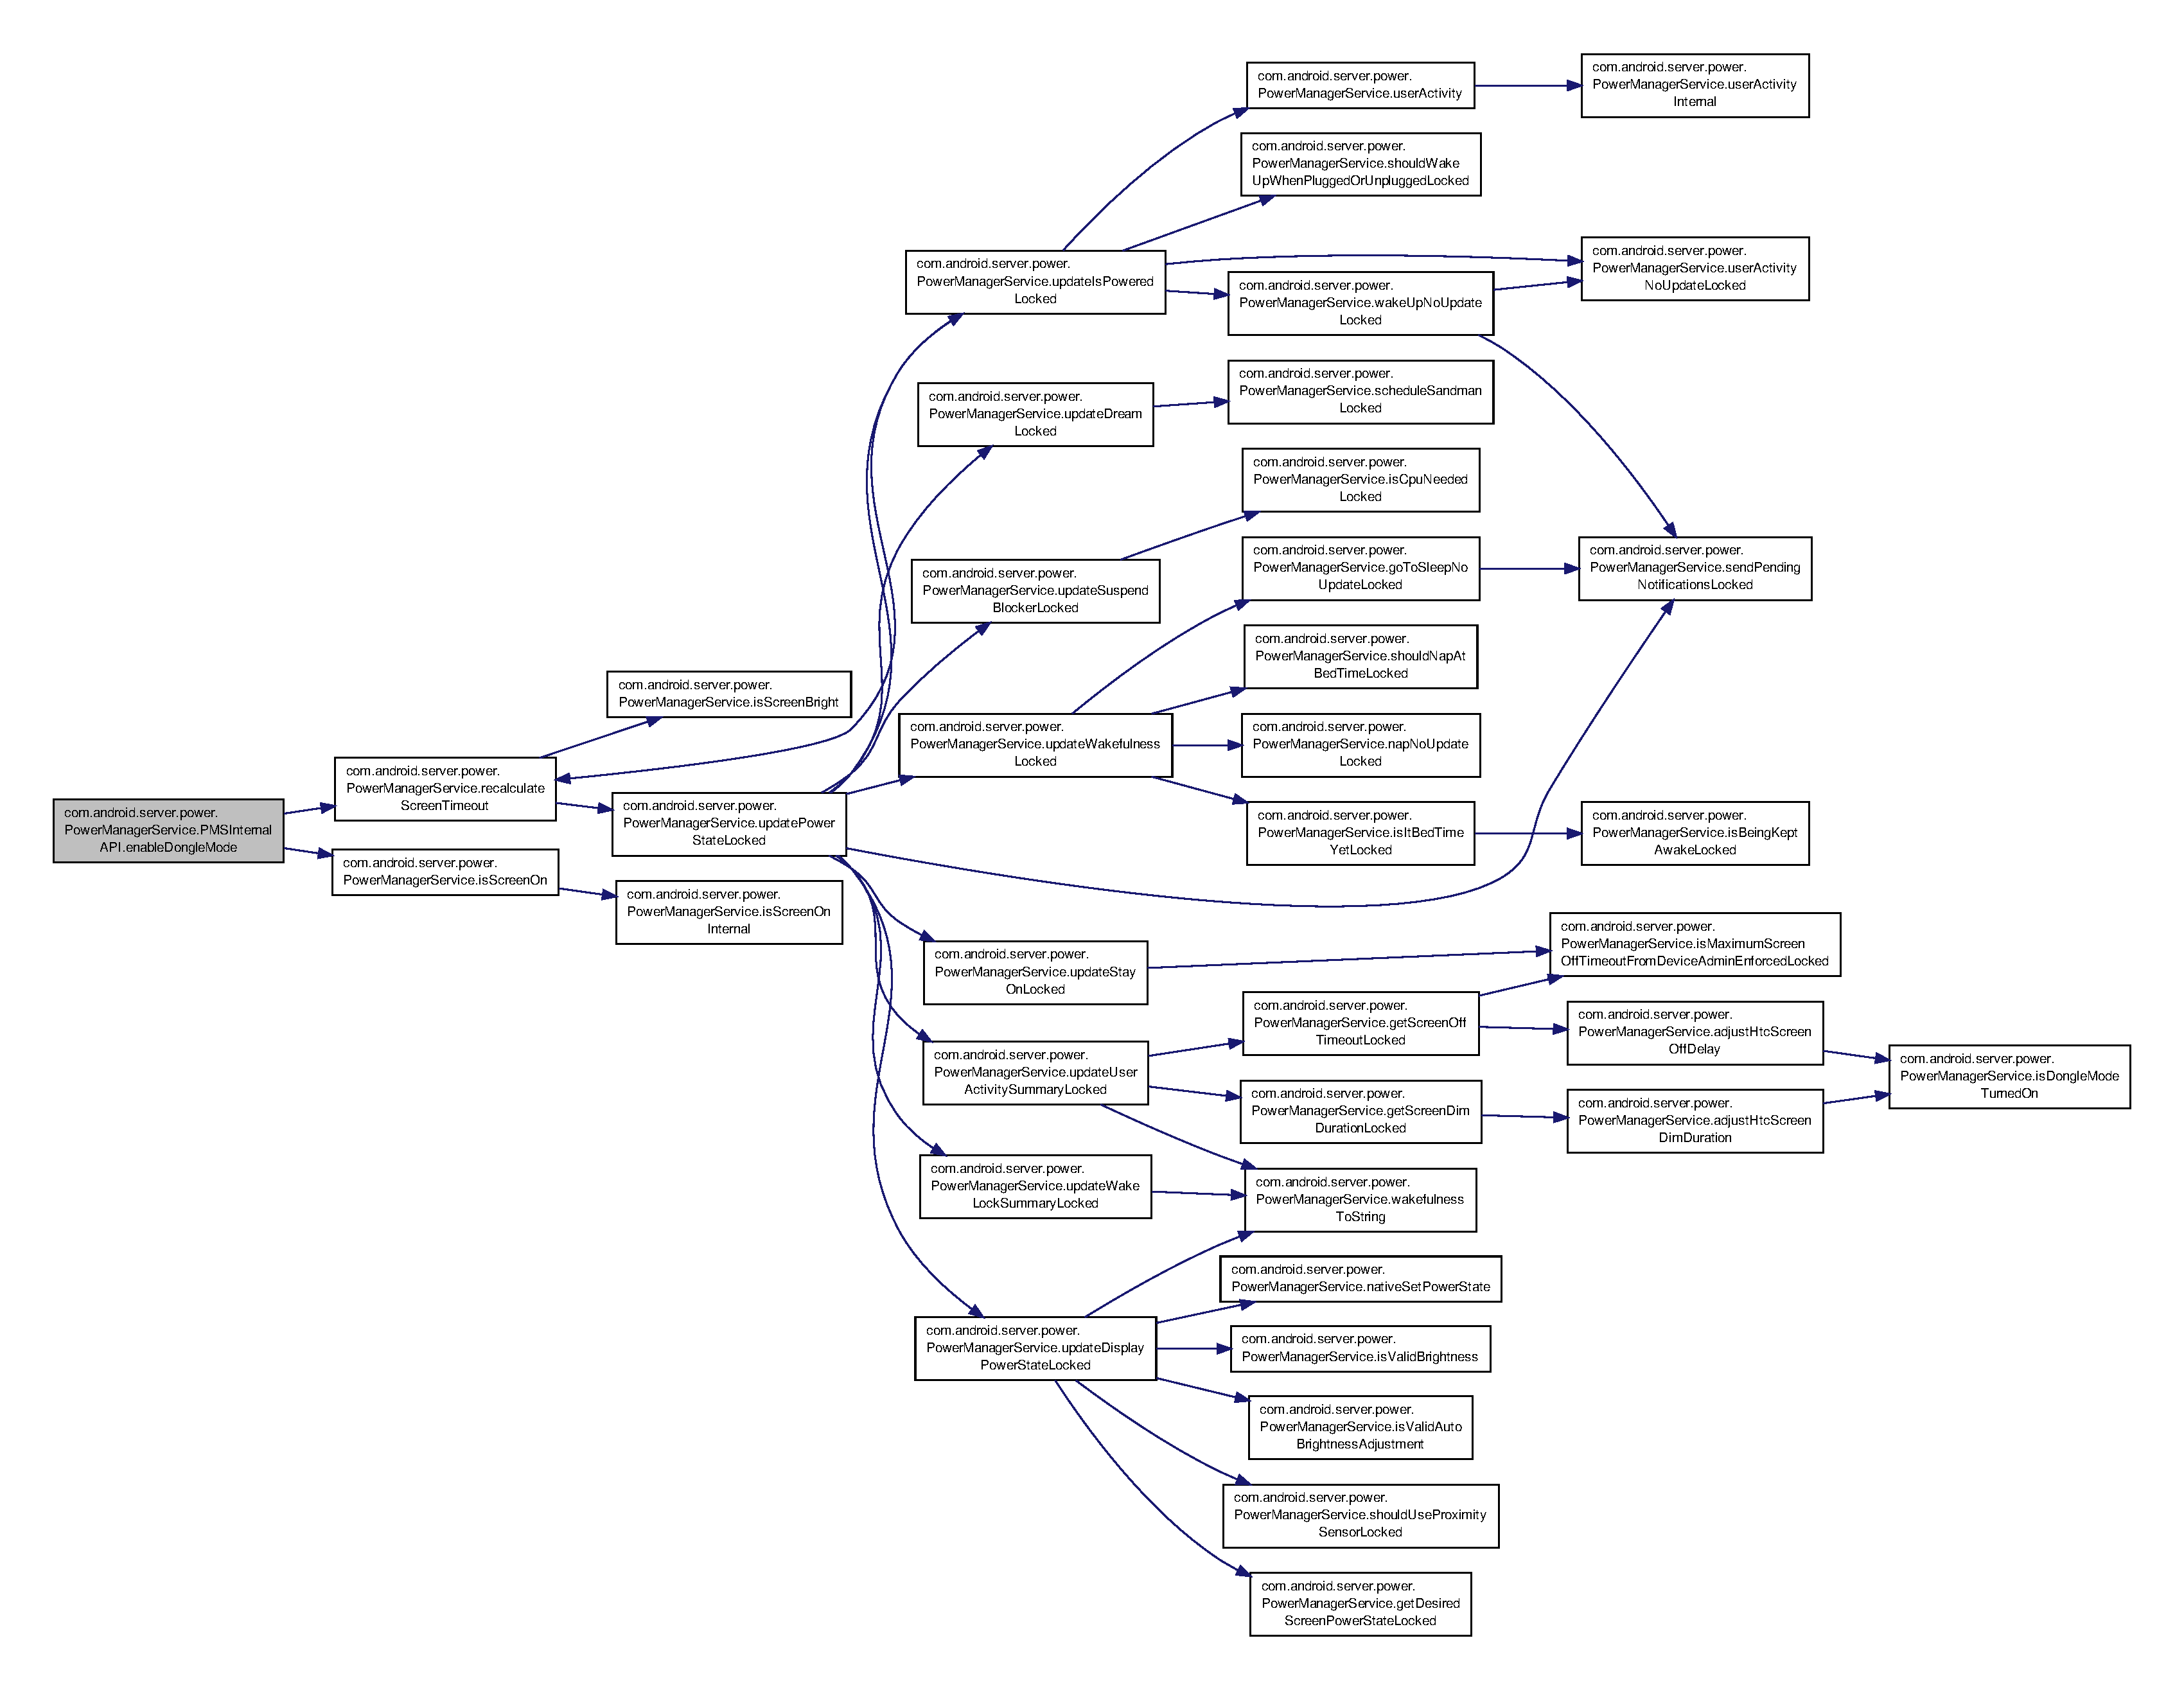
\includegraphics[width=350pt]{classcom_1_1android_1_1server_1_1power_1_1PowerManagerService_1_1PMSInternalAPI_ad786fda0ee177bb56ab41a7d614a1780_cgraph}
\end{center}
\end{figure}


\hypertarget{classcom_1_1android_1_1server_1_1power_1_1PowerManagerService_1_1PMSInternalAPI_aafa8d831439d29a684267d60c946bd10}{\index{com\-::android\-::server\-::power\-::\-Power\-Manager\-Service\-::\-P\-M\-S\-Internal\-A\-P\-I@{com\-::android\-::server\-::power\-::\-Power\-Manager\-Service\-::\-P\-M\-S\-Internal\-A\-P\-I}!lock\-Type@{lock\-Type}}
\index{lock\-Type@{lock\-Type}!com::android::server::power::PowerManagerService::PMSInternalAPI@{com\-::android\-::server\-::power\-::\-Power\-Manager\-Service\-::\-P\-M\-S\-Internal\-A\-P\-I}}
\subsubsection[{lock\-Type}]{\setlength{\rightskip}{0pt plus 5cm}String com.\-android.\-server.\-power.\-Power\-Manager\-Service.\-P\-M\-S\-Internal\-A\-P\-I.\-lock\-Type (
\begin{DoxyParamCaption}
\item[{int}]{flags}
\end{DoxyParamCaption}
)\hspace{0.3cm}{\ttfamily [inline]}, {\ttfamily [protected]}}}\label{classcom_1_1android_1_1server_1_1power_1_1PowerManagerService_1_1PMSInternalAPI_aafa8d831439d29a684267d60c946bd10}
\hypertarget{classcom_1_1android_1_1server_1_1power_1_1PowerManagerService_1_1PMSInternalAPI_a2c21275390cd8f2b1f53cb6dd06c4877}{\index{com\-::android\-::server\-::power\-::\-Power\-Manager\-Service\-::\-P\-M\-S\-Internal\-A\-P\-I@{com\-::android\-::server\-::power\-::\-Power\-Manager\-Service\-::\-P\-M\-S\-Internal\-A\-P\-I}!native\-Acquire\-Cpu\-Ap\-Dvcs\-Wake\-Lock@{native\-Acquire\-Cpu\-Ap\-Dvcs\-Wake\-Lock}}
\index{native\-Acquire\-Cpu\-Ap\-Dvcs\-Wake\-Lock@{native\-Acquire\-Cpu\-Ap\-Dvcs\-Wake\-Lock}!com::android::server::power::PowerManagerService::PMSInternalAPI@{com\-::android\-::server\-::power\-::\-Power\-Manager\-Service\-::\-P\-M\-S\-Internal\-A\-P\-I}}
\subsubsection[{native\-Acquire\-Cpu\-Ap\-Dvcs\-Wake\-Lock}]{\setlength{\rightskip}{0pt plus 5cm}void com.\-android.\-server.\-power.\-Power\-Manager\-Service.\-P\-M\-S\-Internal\-A\-P\-I.\-native\-Acquire\-Cpu\-Ap\-Dvcs\-Wake\-Lock (
\begin{DoxyParamCaption}
{}
\end{DoxyParamCaption}
)\hspace{0.3cm}{\ttfamily [inline]}, {\ttfamily [protected]}}}\label{classcom_1_1android_1_1server_1_1power_1_1PowerManagerService_1_1PMSInternalAPI_a2c21275390cd8f2b1f53cb6dd06c4877}
\hypertarget{classcom_1_1android_1_1server_1_1power_1_1PowerManagerService_1_1PMSInternalAPI_a4db20b5e9bfaa426031e83aa002d7b6e}{\index{com\-::android\-::server\-::power\-::\-Power\-Manager\-Service\-::\-P\-M\-S\-Internal\-A\-P\-I@{com\-::android\-::server\-::power\-::\-Power\-Manager\-Service\-::\-P\-M\-S\-Internal\-A\-P\-I}!native\-Release\-Cpu\-Ap\-Dvcs\-Wake\-Lock@{native\-Release\-Cpu\-Ap\-Dvcs\-Wake\-Lock}}
\index{native\-Release\-Cpu\-Ap\-Dvcs\-Wake\-Lock@{native\-Release\-Cpu\-Ap\-Dvcs\-Wake\-Lock}!com::android::server::power::PowerManagerService::PMSInternalAPI@{com\-::android\-::server\-::power\-::\-Power\-Manager\-Service\-::\-P\-M\-S\-Internal\-A\-P\-I}}
\subsubsection[{native\-Release\-Cpu\-Ap\-Dvcs\-Wake\-Lock}]{\setlength{\rightskip}{0pt plus 5cm}void com.\-android.\-server.\-power.\-Power\-Manager\-Service.\-P\-M\-S\-Internal\-A\-P\-I.\-native\-Release\-Cpu\-Ap\-Dvcs\-Wake\-Lock (
\begin{DoxyParamCaption}
{}
\end{DoxyParamCaption}
)\hspace{0.3cm}{\ttfamily [inline]}, {\ttfamily [protected]}}}\label{classcom_1_1android_1_1server_1_1power_1_1PowerManagerService_1_1PMSInternalAPI_a4db20b5e9bfaa426031e83aa002d7b6e}
\hypertarget{classcom_1_1android_1_1server_1_1power_1_1PowerManagerService_1_1PMSInternalAPI_a8ac36d918efb5363603b8f1af9558902}{\index{com\-::android\-::server\-::power\-::\-Power\-Manager\-Service\-::\-P\-M\-S\-Internal\-A\-P\-I@{com\-::android\-::server\-::power\-::\-Power\-Manager\-Service\-::\-P\-M\-S\-Internal\-A\-P\-I}!set\-Proximity\-State\-With\-Screen\-Off@{set\-Proximity\-State\-With\-Screen\-Off}}
\index{set\-Proximity\-State\-With\-Screen\-Off@{set\-Proximity\-State\-With\-Screen\-Off}!com::android::server::power::PowerManagerService::PMSInternalAPI@{com\-::android\-::server\-::power\-::\-Power\-Manager\-Service\-::\-P\-M\-S\-Internal\-A\-P\-I}}
\subsubsection[{set\-Proximity\-State\-With\-Screen\-Off}]{\setlength{\rightskip}{0pt plus 5cm}void com.\-android.\-server.\-power.\-Power\-Manager\-Service.\-P\-M\-S\-Internal\-A\-P\-I.\-set\-Proximity\-State\-With\-Screen\-Off (
\begin{DoxyParamCaption}
\item[{boolean}]{value}
\end{DoxyParamCaption}
)\hspace{0.3cm}{\ttfamily [inline]}, {\ttfamily [protected]}}}\label{classcom_1_1android_1_1server_1_1power_1_1PowerManagerService_1_1PMSInternalAPI_a8ac36d918efb5363603b8f1af9558902}
\hypertarget{classcom_1_1android_1_1server_1_1power_1_1PowerManagerService_1_1PMSInternalAPI_ae1761f4708d628f8f314c61b116c44eb}{\index{com\-::android\-::server\-::power\-::\-Power\-Manager\-Service\-::\-P\-M\-S\-Internal\-A\-P\-I@{com\-::android\-::server\-::power\-::\-Power\-Manager\-Service\-::\-P\-M\-S\-Internal\-A\-P\-I}!set\-Screen\-Brightness\-Mode@{set\-Screen\-Brightness\-Mode}}
\index{set\-Screen\-Brightness\-Mode@{set\-Screen\-Brightness\-Mode}!com::android::server::power::PowerManagerService::PMSInternalAPI@{com\-::android\-::server\-::power\-::\-Power\-Manager\-Service\-::\-P\-M\-S\-Internal\-A\-P\-I}}
\subsubsection[{set\-Screen\-Brightness\-Mode}]{\setlength{\rightskip}{0pt plus 5cm}void com.\-android.\-server.\-power.\-Power\-Manager\-Service.\-P\-M\-S\-Internal\-A\-P\-I.\-set\-Screen\-Brightness\-Mode (
\begin{DoxyParamCaption}
\item[{int}]{mode}
\end{DoxyParamCaption}
)\hspace{0.3cm}{\ttfamily [inline]}, {\ttfamily [protected]}}}\label{classcom_1_1android_1_1server_1_1power_1_1PowerManagerService_1_1PMSInternalAPI_ae1761f4708d628f8f314c61b116c44eb}


Here is the call graph for this function\-:
\nopagebreak
\begin{figure}[H]
\begin{center}
\leavevmode
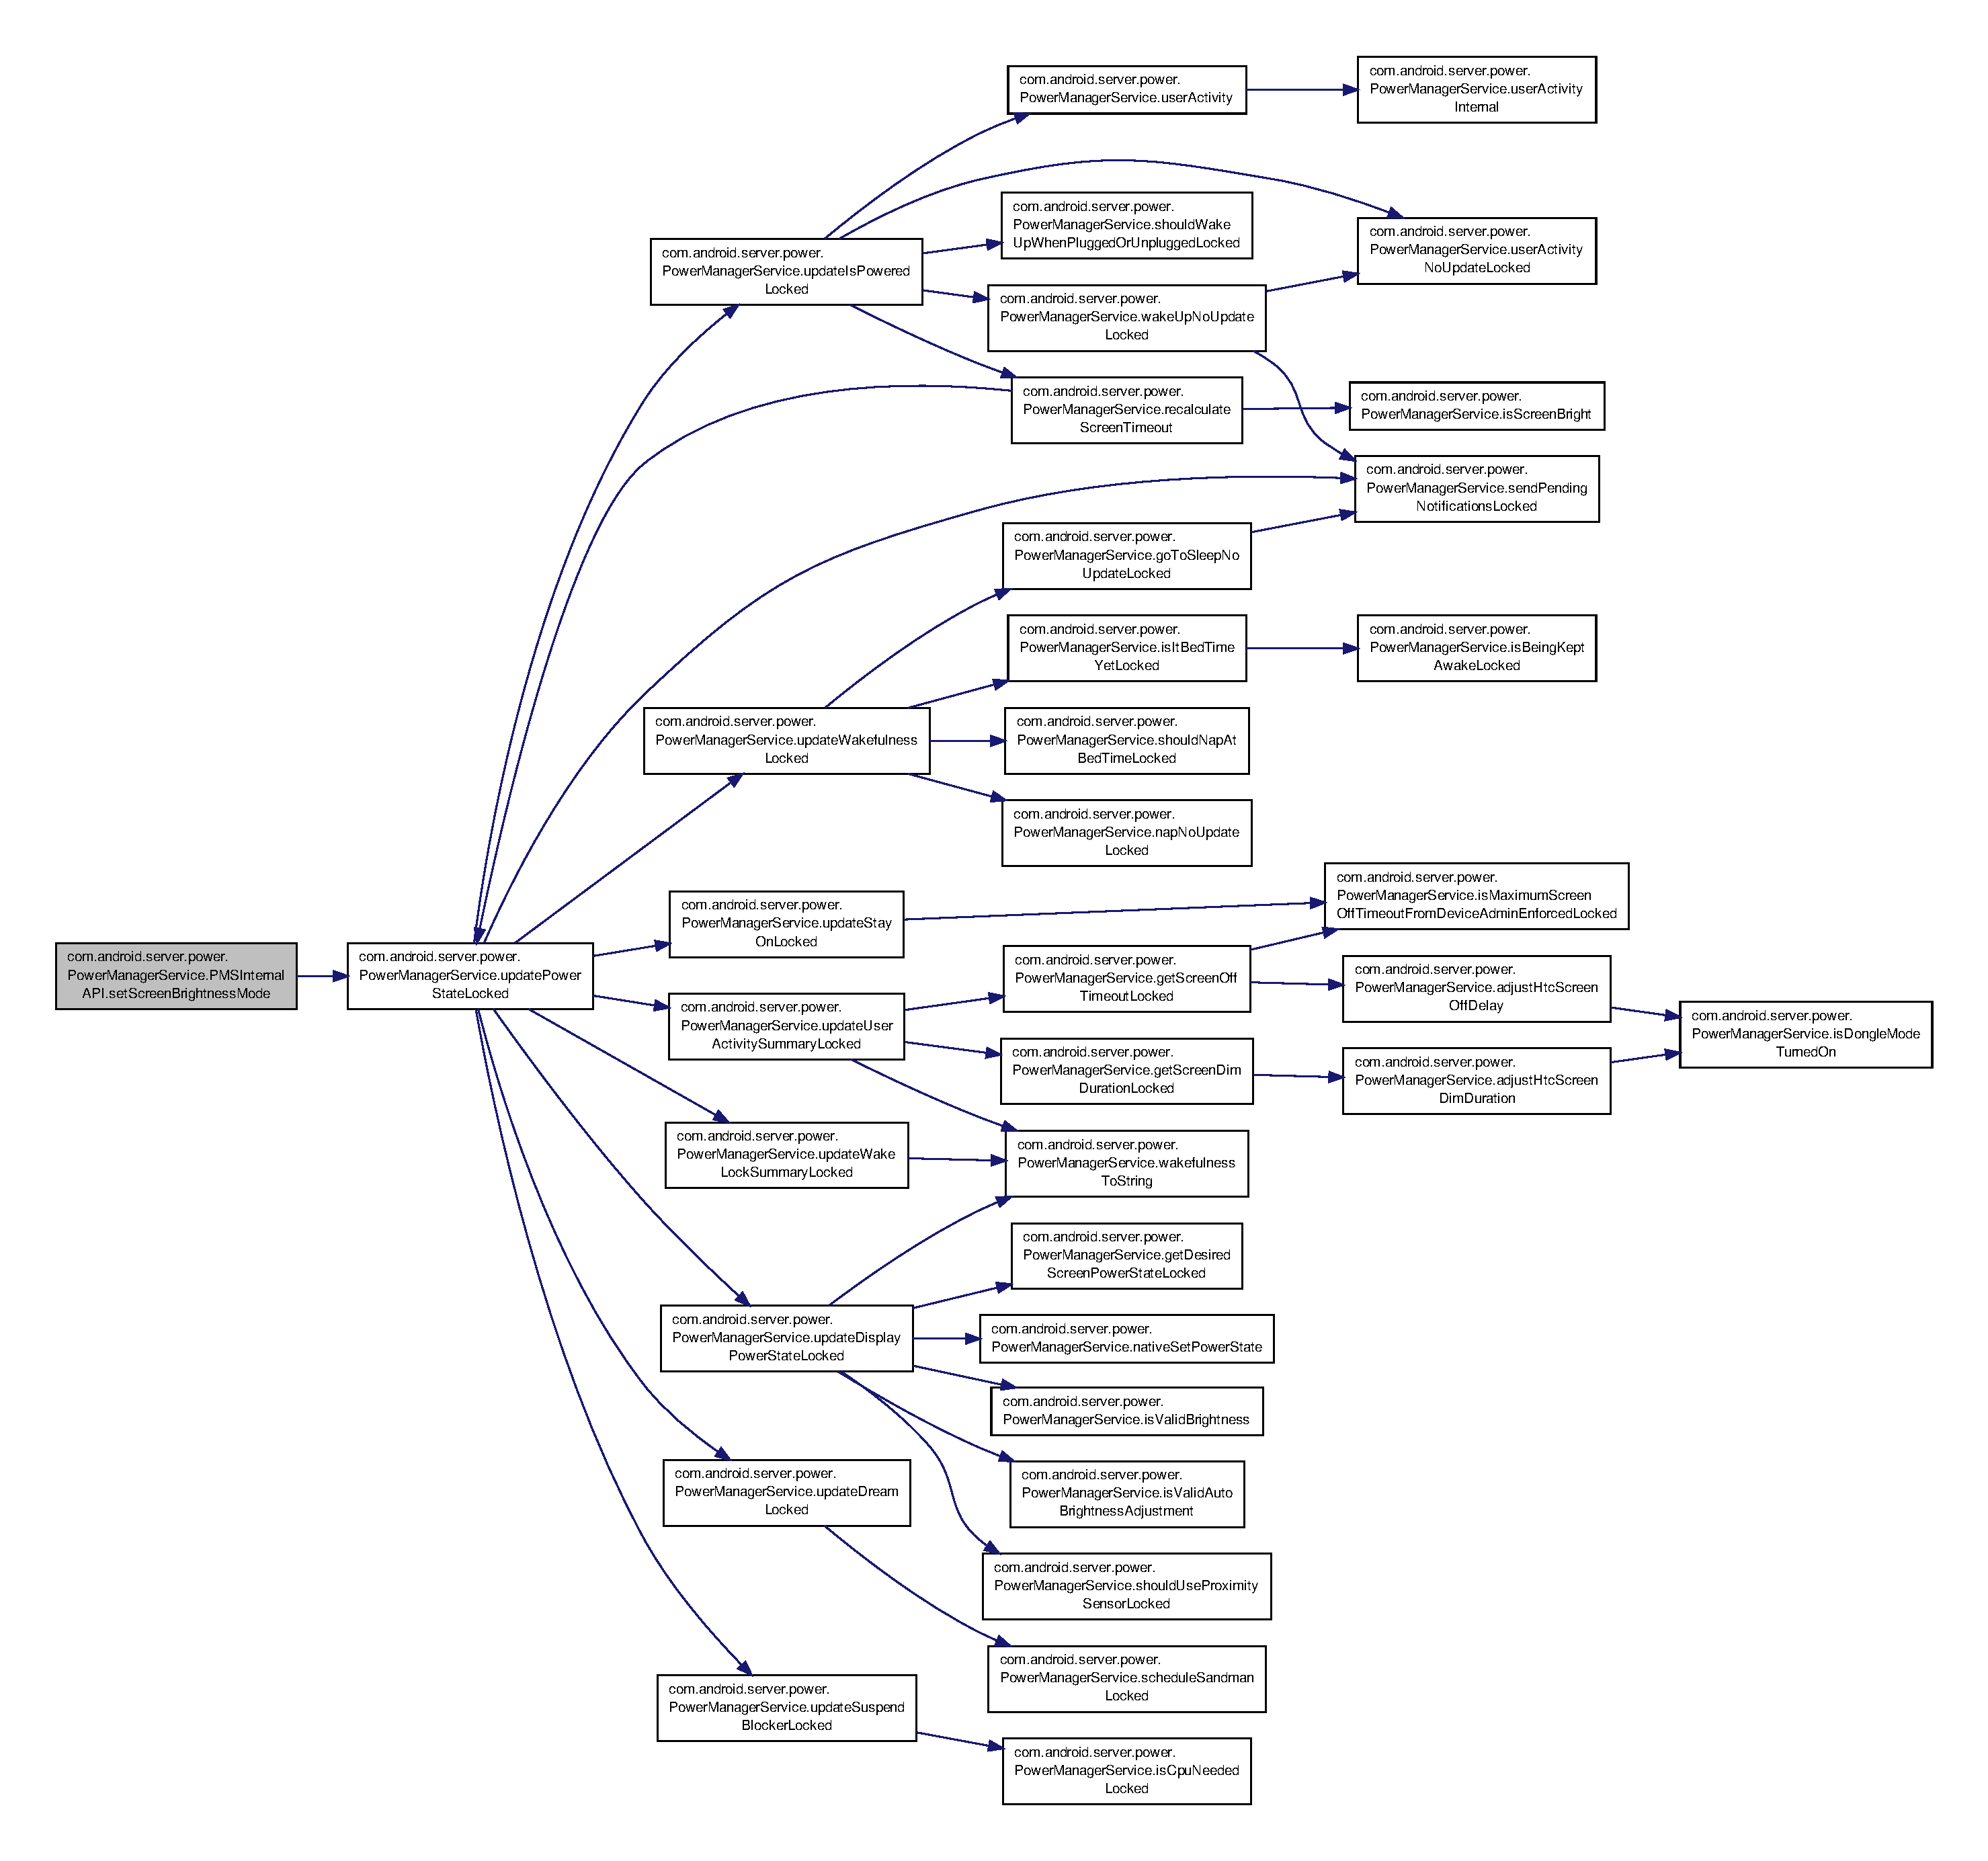
\includegraphics[width=350pt]{classcom_1_1android_1_1server_1_1power_1_1PowerManagerService_1_1PMSInternalAPI_ae1761f4708d628f8f314c61b116c44eb_cgraph}
\end{center}
\end{figure}




The documentation for this class was generated from the following file\-:\begin{DoxyCompactItemize}
\item 
\hyperlink{PowerManagerService_8java}{Power\-Manager\-Service.\-java}\end{DoxyCompactItemize}

\hypertarget{classcom_1_1android_1_1server_1_1power_1_1PowerManagerService_1_1PowerManagerHandler}{\section{com.\-android.\-server.\-power.\-Power\-Manager\-Service.\-Power\-Manager\-Handler Class Reference}
\label{classcom_1_1android_1_1server_1_1power_1_1PowerManagerService_1_1PowerManagerHandler}\index{com.\-android.\-server.\-power.\-Power\-Manager\-Service.\-Power\-Manager\-Handler@{com.\-android.\-server.\-power.\-Power\-Manager\-Service.\-Power\-Manager\-Handler}}
}


Inheritance diagram for com.\-android.\-server.\-power.\-Power\-Manager\-Service.\-Power\-Manager\-Handler\-:
\nopagebreak
\begin{figure}[H]
\begin{center}
\leavevmode
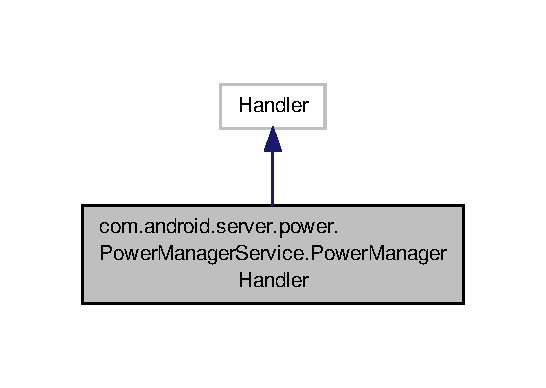
\includegraphics[width=262pt]{classcom_1_1android_1_1server_1_1power_1_1PowerManagerService_1_1PowerManagerHandler__inherit__graph}
\end{center}
\end{figure}


Collaboration diagram for com.\-android.\-server.\-power.\-Power\-Manager\-Service.\-Power\-Manager\-Handler\-:
\nopagebreak
\begin{figure}[H]
\begin{center}
\leavevmode
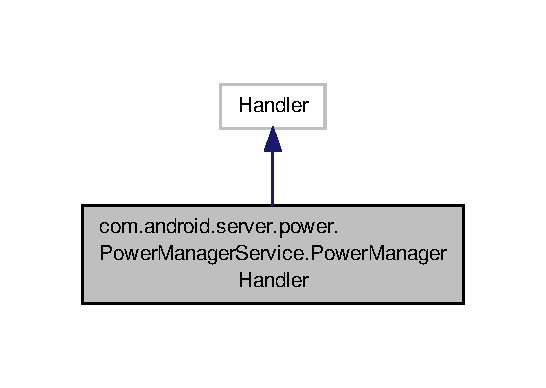
\includegraphics[width=262pt]{classcom_1_1android_1_1server_1_1power_1_1PowerManagerService_1_1PowerManagerHandler__coll__graph}
\end{center}
\end{figure}
\subsection*{Public Member Functions}
\begin{DoxyCompactItemize}
\item 
\hyperlink{classcom_1_1android_1_1server_1_1power_1_1PowerManagerService_1_1PowerManagerHandler_aaf7c53c19097c32845d5224322f3fcaf}{Power\-Manager\-Handler} (Looper looper)
\item 
void \hyperlink{classcom_1_1android_1_1server_1_1power_1_1PowerManagerService_1_1PowerManagerHandler_a34b202051e8ac690bc18055a069f3664}{handle\-Message} (Message msg)
\end{DoxyCompactItemize}


\subsection{Detailed Description}
Handler for asynchronous operations performed by the power manager. 

\subsection{Constructor \& Destructor Documentation}
\hypertarget{classcom_1_1android_1_1server_1_1power_1_1PowerManagerService_1_1PowerManagerHandler_aaf7c53c19097c32845d5224322f3fcaf}{\index{com\-::android\-::server\-::power\-::\-Power\-Manager\-Service\-::\-Power\-Manager\-Handler@{com\-::android\-::server\-::power\-::\-Power\-Manager\-Service\-::\-Power\-Manager\-Handler}!Power\-Manager\-Handler@{Power\-Manager\-Handler}}
\index{Power\-Manager\-Handler@{Power\-Manager\-Handler}!com::android::server::power::PowerManagerService::PowerManagerHandler@{com\-::android\-::server\-::power\-::\-Power\-Manager\-Service\-::\-Power\-Manager\-Handler}}
\subsubsection[{Power\-Manager\-Handler}]{\setlength{\rightskip}{0pt plus 5cm}com.\-android.\-server.\-power.\-Power\-Manager\-Service.\-Power\-Manager\-Handler.\-Power\-Manager\-Handler (
\begin{DoxyParamCaption}
\item[{Looper}]{looper}
\end{DoxyParamCaption}
)\hspace{0.3cm}{\ttfamily [inline]}}}\label{classcom_1_1android_1_1server_1_1power_1_1PowerManagerService_1_1PowerManagerHandler_aaf7c53c19097c32845d5224322f3fcaf}


\subsection{Member Function Documentation}
\hypertarget{classcom_1_1android_1_1server_1_1power_1_1PowerManagerService_1_1PowerManagerHandler_a34b202051e8ac690bc18055a069f3664}{\index{com\-::android\-::server\-::power\-::\-Power\-Manager\-Service\-::\-Power\-Manager\-Handler@{com\-::android\-::server\-::power\-::\-Power\-Manager\-Service\-::\-Power\-Manager\-Handler}!handle\-Message@{handle\-Message}}
\index{handle\-Message@{handle\-Message}!com::android::server::power::PowerManagerService::PowerManagerHandler@{com\-::android\-::server\-::power\-::\-Power\-Manager\-Service\-::\-Power\-Manager\-Handler}}
\subsubsection[{handle\-Message}]{\setlength{\rightskip}{0pt plus 5cm}void com.\-android.\-server.\-power.\-Power\-Manager\-Service.\-Power\-Manager\-Handler.\-handle\-Message (
\begin{DoxyParamCaption}
\item[{Message}]{msg}
\end{DoxyParamCaption}
)\hspace{0.3cm}{\ttfamily [inline]}}}\label{classcom_1_1android_1_1server_1_1power_1_1PowerManagerService_1_1PowerManagerHandler_a34b202051e8ac690bc18055a069f3664}


Here is the call graph for this function\-:
\nopagebreak
\begin{figure}[H]
\begin{center}
\leavevmode
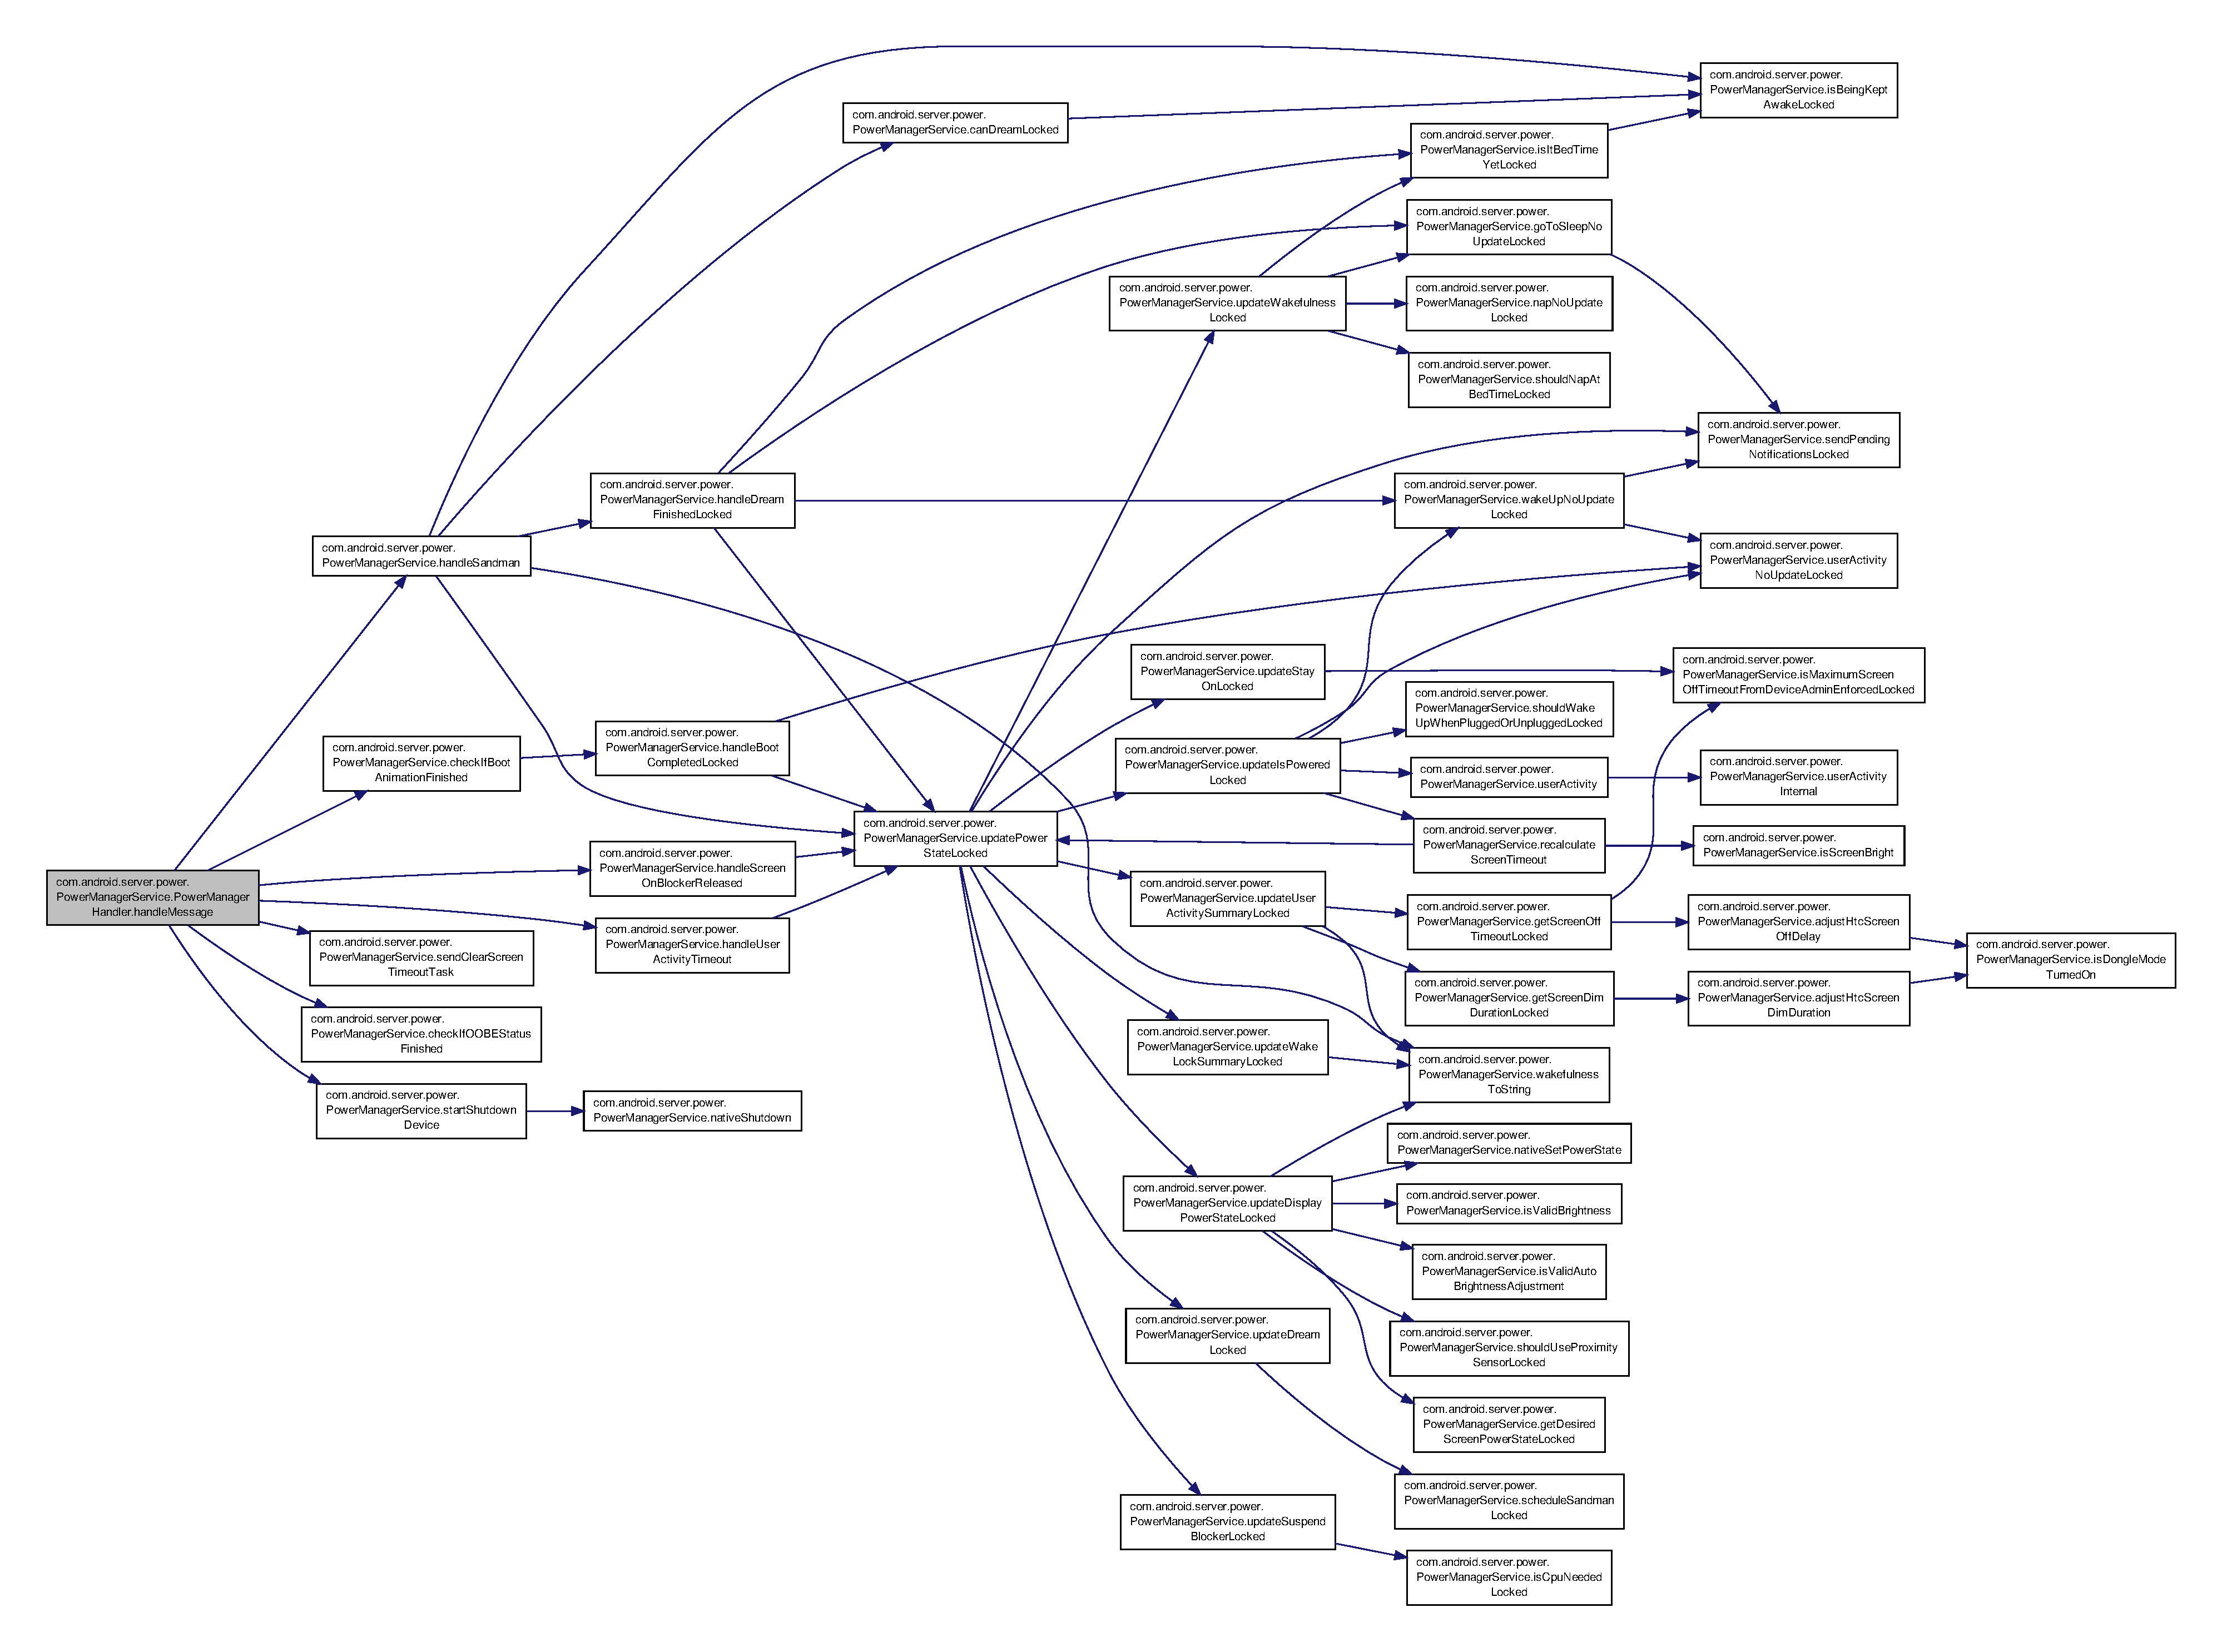
\includegraphics[width=350pt]{classcom_1_1android_1_1server_1_1power_1_1PowerManagerService_1_1PowerManagerHandler_a34b202051e8ac690bc18055a069f3664_cgraph}
\end{center}
\end{figure}




The documentation for this class was generated from the following file\-:\begin{DoxyCompactItemize}
\item 
\hyperlink{PowerManagerService_8java}{Power\-Manager\-Service.\-java}\end{DoxyCompactItemize}

\hypertarget{classcom_1_1android_1_1server_1_1power_1_1PowerManagerService}{\section{com.\-android.\-server.\-power.\-Power\-Manager\-Service Class Reference}
\label{classcom_1_1android_1_1server_1_1power_1_1PowerManagerService}\index{com.\-android.\-server.\-power.\-Power\-Manager\-Service@{com.\-android.\-server.\-power.\-Power\-Manager\-Service}}
}


Inheritance diagram for com.\-android.\-server.\-power.\-Power\-Manager\-Service\-:
\nopagebreak
\begin{figure}[H]
\begin{center}
\leavevmode
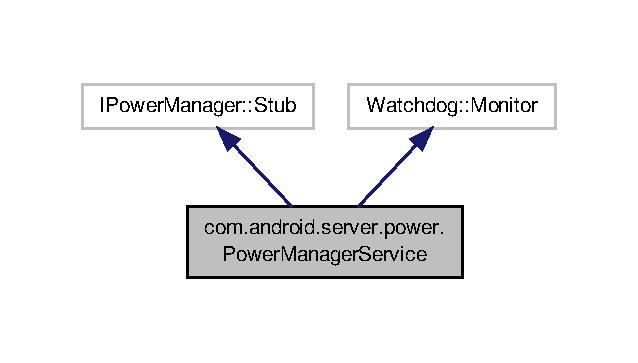
\includegraphics[width=306pt]{classcom_1_1android_1_1server_1_1power_1_1PowerManagerService__inherit__graph}
\end{center}
\end{figure}


Collaboration diagram for com.\-android.\-server.\-power.\-Power\-Manager\-Service\-:
\nopagebreak
\begin{figure}[H]
\begin{center}
\leavevmode
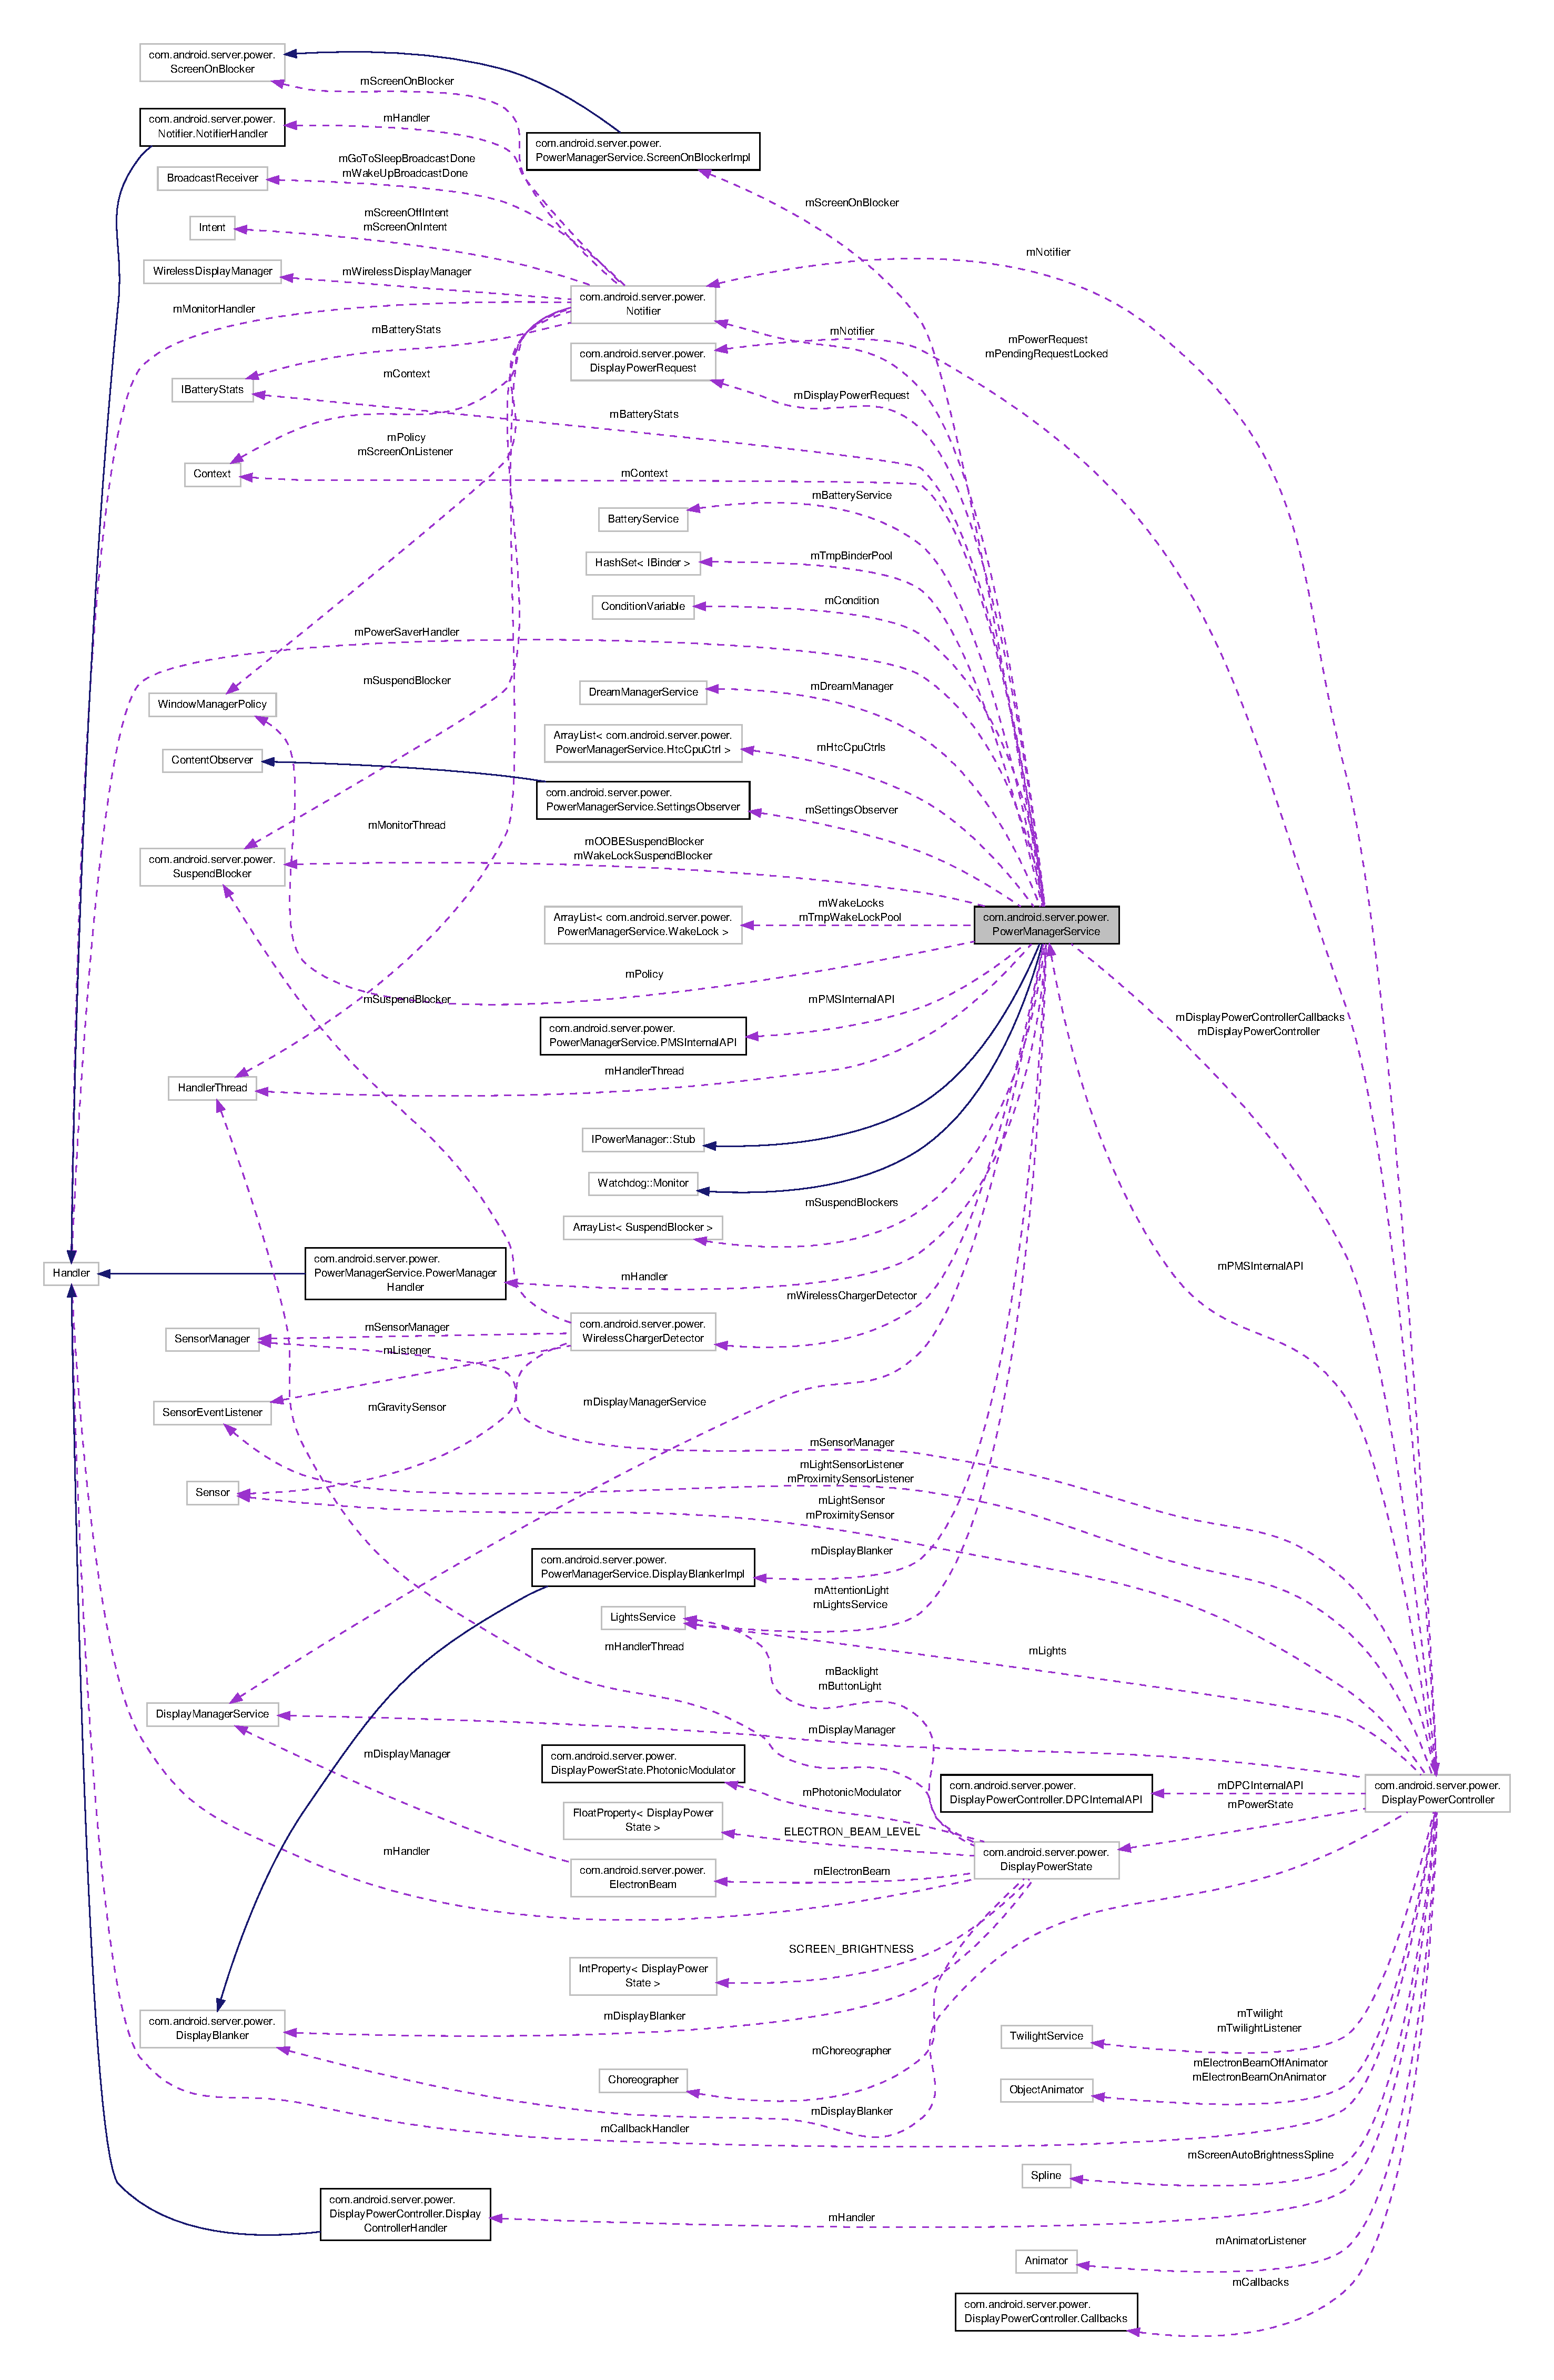
\includegraphics[width=350pt]{classcom_1_1android_1_1server_1_1power_1_1PowerManagerService__coll__graph}
\end{center}
\end{figure}
\subsection*{Classes}
\begin{DoxyCompactItemize}
\item 
class \hyperlink{classcom_1_1android_1_1server_1_1power_1_1PowerManagerService_1_1BatteryReceiver}{Battery\-Receiver}
\item 
class \hyperlink{classcom_1_1android_1_1server_1_1power_1_1PowerManagerService_1_1BootCompletedReceiver}{Boot\-Completed\-Receiver}
\item 
class \hyperlink{classcom_1_1android_1_1server_1_1power_1_1PowerManagerService_1_1DisplayBlankerImpl}{Display\-Blanker\-Impl}
\item 
class \hyperlink{classcom_1_1android_1_1server_1_1power_1_1PowerManagerService_1_1DockReceiver}{Dock\-Receiver}
\item 
class \hyperlink{classcom_1_1android_1_1server_1_1power_1_1PowerManagerService_1_1DreamReceiver}{Dream\-Receiver}
\item 
class \hyperlink{classcom_1_1android_1_1server_1_1power_1_1PowerManagerService_1_1HtcCpuCtrl}{Htc\-Cpu\-Ctrl}
\item 
class \hyperlink{classcom_1_1android_1_1server_1_1power_1_1PowerManagerService_1_1OOBETimeoutReceiver}{O\-O\-B\-E\-Timeout\-Receiver}
\item 
class \hyperlink{classcom_1_1android_1_1server_1_1power_1_1PowerManagerService_1_1PMSInternalAPI}{P\-M\-S\-Internal\-A\-P\-I}
\item 
class \hyperlink{classcom_1_1android_1_1server_1_1power_1_1PowerManagerService_1_1PowerManagerHandler}{Power\-Manager\-Handler}
\item 
class \hyperlink{classcom_1_1android_1_1server_1_1power_1_1PowerManagerService_1_1ScreenOnBlockerImpl}{Screen\-On\-Blocker\-Impl}
\item 
class \hyperlink{classcom_1_1android_1_1server_1_1power_1_1PowerManagerService_1_1SettingsObserver}{Settings\-Observer}
\item 
class \hyperlink{classcom_1_1android_1_1server_1_1power_1_1PowerManagerService_1_1SuspendBlockerImpl}{Suspend\-Blocker\-Impl}
\item 
class \hyperlink{classcom_1_1android_1_1server_1_1power_1_1PowerManagerService_1_1UserSwitchedReceiver}{User\-Switched\-Receiver}
\item 
class \hyperlink{classcom_1_1android_1_1server_1_1power_1_1PowerManagerService_1_1WakeLock}{Wake\-Lock}
\end{DoxyCompactItemize}
\subsection*{Public Member Functions}
\begin{DoxyCompactItemize}
\item 
\hyperlink{classcom_1_1android_1_1server_1_1power_1_1PowerManagerService_af61f43046957912e62237da840197b84}{Power\-Manager\-Service} ()
\item 
void \hyperlink{classcom_1_1android_1_1server_1_1power_1_1PowerManagerService_af4ef6caf8d8906988b32470167669ec6}{init} (Context context, Lights\-Service ls, Activity\-Manager\-Service am, Battery\-Service bs, I\-Battery\-Stats bss, Display\-Manager\-Service dm)
\item 
void \hyperlink{classcom_1_1android_1_1server_1_1power_1_1PowerManagerService_a9c258b7f4cfc587dfda695b47f75be9e}{set\-Policy} (Window\-Manager\-Policy policy)
\item 
void \hyperlink{classcom_1_1android_1_1server_1_1power_1_1PowerManagerService_a99479445bbbc687684f583c69a9ba39b}{system\-Ready} (Twilight\-Service twilight, Dream\-Manager\-Service dream\-Manager)
\item 
void \hyperlink{classcom_1_1android_1_1server_1_1power_1_1PowerManagerService_afeb6fabbab5aed353735777a05becf3f}{acquire\-Wake\-Lock} (I\-Binder lock, int flags, String tag, Work\-Source ws)
\item 
void \hyperlink{classcom_1_1android_1_1server_1_1power_1_1PowerManagerService_a92faede593a057488165d627041ee2c2}{acquire\-Htc\-Cpu\-Ctrl} (int flags, I\-Binder lock, String tag, Work\-Source ws, int level)
\item 
void \hyperlink{classcom_1_1android_1_1server_1_1power_1_1PowerManagerService_ab74ce4c78bc9df9d5a2af05a511487cb}{release\-Wake\-Lock} (I\-Binder lock, int flags)
\item 
void \hyperlink{classcom_1_1android_1_1server_1_1power_1_1PowerManagerService_accfbc813d8ba64b9672c5053862013f8}{release\-Htc\-Cpu\-Ctrl} (I\-Binder lock, int flags)
\item 
void \hyperlink{classcom_1_1android_1_1server_1_1power_1_1PowerManagerService_acc2cb88d3e5e70d961b404a2a7bb0483}{update\-Wake\-Lock\-Work\-Source} (I\-Binder lock, Work\-Source ws)
\item 
void \hyperlink{classcom_1_1android_1_1server_1_1power_1_1PowerManagerService_a1cf4fcda2fc126a0e8f7a1fed9f03574}{update\-Htc\-Cpu\-Ctrl\-Work\-Source} (I\-Binder lock, Work\-Source ws)
\item 
boolean \hyperlink{classcom_1_1android_1_1server_1_1power_1_1PowerManagerService_ad611e00d7d64d1d0f87ae76be7446b73}{is\-Wake\-Lock\-Level\-Supported} (int level)
\item 
void \hyperlink{classcom_1_1android_1_1server_1_1power_1_1PowerManagerService_a7b38d6b64ca48c42701d423494675c64}{user\-Activity} (long event\-Time, int event, int flags)
\item 
void \hyperlink{classcom_1_1android_1_1server_1_1power_1_1PowerManagerService_ab4216ff9e76a76254a64f4097becdf32}{wake\-Up} (long event\-Time)
\item 
void \hyperlink{classcom_1_1android_1_1server_1_1power_1_1PowerManagerService_acbf0e30e8cf85ab34974082d98321858}{go\-To\-Sleep\-For\-Shutdown} (long time, int reason)
\item 
boolean \hyperlink{classcom_1_1android_1_1server_1_1power_1_1PowerManagerService_a9a132717d1b3e6ab90aa5383229db1bf}{get\-Native\-Set\-Auto\-Suspend\-Done} ()
\item 
void \hyperlink{classcom_1_1android_1_1server_1_1power_1_1PowerManagerService_a988e232d9be4d9b76c69a386a9b2bddd}{go\-To\-Sleep} (long event\-Time, int reason)
\item 
void \hyperlink{classcom_1_1android_1_1server_1_1power_1_1PowerManagerService_a3838189fff42aad9929fd3b0493264cf}{nap} (long event\-Time)
\item 
void \hyperlink{classcom_1_1android_1_1server_1_1power_1_1PowerManagerService_ac3f7d0be2dfe51cbc4f4adfd11a8c58a}{user\-Activity\-With\-Screen\-Delay} (long when, boolean no\-Change\-Lights, final int keylight\-Delay, final int dim\-Delay, final int screen\-Off\-Delay)
\item 
void \hyperlink{classcom_1_1android_1_1server_1_1power_1_1PowerManagerService_a2c7c87f894a98724d0f917e49aab0638}{customize\-Screen\-Off\-Delay\-\_\-\-Once} (final int screen\-Off\-Delay, final boolean calc\-Remaining)
\item 
void \hyperlink{classcom_1_1android_1_1server_1_1power_1_1PowerManagerService_aaee5f3f019a74b2bf1099b85a61758a8}{customize\-Screen\-Off\-Delay\-\_\-\-Always} (final int screen\-Off\-Delay, final boolean calc\-Remaining)
\item 
void \hyperlink{classcom_1_1android_1_1server_1_1power_1_1PowerManagerService_a2f0c0d1672e980162d6e58e129934ae5}{customize\-Screen\-Off\-Delay\-\_\-\-System} (final int screen\-Off\-Delay, final boolean calc\-Remaining)
\item 
boolean \hyperlink{classcom_1_1android_1_1server_1_1power_1_1PowerManagerService_a7d58ccc5c065d016a6574f5ccb0485e3}{is\-Screen\-On} ()
\item 
boolean \hyperlink{classcom_1_1android_1_1server_1_1power_1_1PowerManagerService_a34fe3f3ab59f1cd9731cfb2eefa4431c}{is\-Actual\-Screen\-On} ()
\item 
void \hyperlink{classcom_1_1android_1_1server_1_1power_1_1PowerManagerService_a95eb0d786da21973541e4792885aa7b5}{reboot} (boolean confirm, String reason, boolean wait)
\item 
void \hyperlink{classcom_1_1android_1_1server_1_1power_1_1PowerManagerService_a1ae14154de05bc246283fa01687e4fc8}{shutdown} (boolean confirm, boolean wait)
\item 
void \hyperlink{classcom_1_1android_1_1server_1_1power_1_1PowerManagerService_a98ff223785ece7b9c30e8ecca67b7867}{crash} (String message)
\item 
void \hyperlink{classcom_1_1android_1_1server_1_1power_1_1PowerManagerService_ab81abded4b2577f62081dcf7d9659630}{set\-Stay\-On\-Setting} (int val)
\item 
void \hyperlink{classcom_1_1android_1_1server_1_1power_1_1PowerManagerService_a25ab9b6fb59613eb589fc4ab30ce21fd}{set\-Maximum\-Screen\-Off\-Timeout\-From\-Device\-Admin} (int time\-Ms)
\item 
void \hyperlink{classcom_1_1android_1_1server_1_1power_1_1PowerManagerService_a71af17d5f1b3caa01229f5a4c23c5e94}{set\-Attention\-Light} (boolean on, int color)
\item 
long \hyperlink{classcom_1_1android_1_1server_1_1power_1_1PowerManagerService_a057c323112fdc09f4b71f1d34e33996c}{time\-Since\-Screen\-Was\-Last\-On} ()
\item 
void \hyperlink{classcom_1_1android_1_1server_1_1power_1_1PowerManagerService_a5633964c7598882ca1c50f469d05f7fa}{set\-Screen\-Brightness\-Override\-From\-Window\-Manager} (int brightness)
\item 
void \hyperlink{classcom_1_1android_1_1server_1_1power_1_1PowerManagerService_a87213a2ce0f6b8a6dc478cd634979299}{set\-Button\-Brightness\-Override\-From\-Window\-Manager} (int brightness)
\item 
void \hyperlink{classcom_1_1android_1_1server_1_1power_1_1PowerManagerService_a14f403354cd8ee18ecc8a4d51263dc69}{set\-User\-Activity\-Timeout\-Override\-From\-Window\-Manager} (long timeout\-Millis)
\item 
void \hyperlink{classcom_1_1android_1_1server_1_1power_1_1PowerManagerService_a24f557fb66d9e937ad23747e6d89fd1d}{set\-Temporary\-Screen\-Brightness\-Setting\-Override} (int brightness)
\item 
void \hyperlink{classcom_1_1android_1_1server_1_1power_1_1PowerManagerService_ac6f361dfa708a4a0a96085f5117ef57a}{set\-Temporary\-Screen\-Auto\-Brightness\-Adjustment\-Setting\-Override} (float adj)
\item 
void \hyperlink{classcom_1_1android_1_1server_1_1power_1_1PowerManagerService_a3606a2b867c37574e88495a9839c65a8}{low\-Level\-Shutdown\-\_\-system} ()
\item 
void \hyperlink{classcom_1_1android_1_1server_1_1power_1_1PowerManagerService_a8ed23cef4d238b9c8079531213c3bb00}{low\-Level\-Reboot\-\_\-system} (String reason)
\item 
void \hyperlink{classcom_1_1android_1_1server_1_1power_1_1PowerManagerService_a199ecf0e643121b352dd497d5718049c}{low\-Level\-Shutdown\-E\-F\-S\-Sync} ()
\item 
void \hyperlink{classcom_1_1android_1_1server_1_1power_1_1PowerManagerService_a4dd8be1755b3f0cab3f8599e86379983}{low\-Level\-Shutdown\-E\-F\-S\-Sync\-\_\-wait} (int ms\-Timeout)
\item 
boolean \hyperlink{classcom_1_1android_1_1server_1_1power_1_1PowerManagerService_ae91981409b5fa94b9faaab5920f6c8ca}{wipe\-System} (byte\mbox{[}$\,$\mbox{]} imei, byte\mbox{[}$\,$\mbox{]} enc\-Msg)
\item 
void \hyperlink{classcom_1_1android_1_1server_1_1power_1_1PowerManagerService_ad0363a56b5777cd188abd1310bcd5fc2}{monitor} ()
\item 
void \hyperlink{classcom_1_1android_1_1server_1_1power_1_1PowerManagerService_a1980f91e957fd3661e615910f91b0778}{watchdog} ()
\begin{DoxyCompactList}\small\item\em H\-T\-C\-: trigger watchdog timeout. \end{DoxyCompactList}\item 
void \hyperlink{classcom_1_1android_1_1server_1_1power_1_1PowerManagerService_a5025e7fa3ab11ff7e6393430f4431989}{set\-Abl\-Active} (int on)
\item 
int \hyperlink{classcom_1_1android_1_1server_1_1power_1_1PowerManagerService_a9c8afb471b72eb9d448e1fc4a1649bbb}{fetch\-Current\-Brightness\-Value} ()
\item 
boolean \hyperlink{classcom_1_1android_1_1server_1_1power_1_1PowerManagerService_adf51be5faae092d09d844c34f57e2a50}{get\-Proximity\-Sensor\-Active} ()
\item 
int\mbox{[}$\,$\mbox{]} \hyperlink{classcom_1_1android_1_1server_1_1power_1_1PowerManagerService_a550a64aebe82e8c26233a2c334111aa2}{get\-Light\-Sensor\-Table\-Values} ()
\item 
void \hyperlink{classcom_1_1android_1_1server_1_1power_1_1PowerManagerService_a975fbb3607c855f15292e7a0e2896a80}{set\-Pen\-Menu\-Button\-Led} (int pen\-Button\-Led)
\item 
void \hyperlink{classcom_1_1android_1_1server_1_1power_1_1PowerManagerService_a70eb76239bdfc13c354eb17a1250bfb1}{set\-Orientation} (int orientation)
\item 
void \hyperlink{classcom_1_1android_1_1server_1_1power_1_1PowerManagerService_a2c37aeb0e678ef2884b9c19580f7834b}{inform\-O\-O\-B\-E\-Status\-Change} (boolean status)
\end{DoxyCompactItemize}
\subsection*{Static Public Member Functions}
\begin{DoxyCompactItemize}
\item 
static native void \hyperlink{classcom_1_1android_1_1server_1_1power_1_1PowerManagerService_a46a637df6dae5ddc05b11c2328e8fe84}{native\-Acquire\-Cpu\-Perf\-Wake\-Lock} ()
\item 
static native void \hyperlink{classcom_1_1android_1_1server_1_1power_1_1PowerManagerService_ad615daf1f57b0513b021d424ff7ec50c}{native\-Release\-Cpu\-Perf\-Wake\-Lock} ()
\item 
static void \hyperlink{classcom_1_1android_1_1server_1_1power_1_1PowerManagerService_a3dc7ceb97425c68eeb6fe18f83afc962}{low\-Level\-Shutdown} ()
\item 
static void \hyperlink{classcom_1_1android_1_1server_1_1power_1_1PowerManagerService_a3b4db5d2610f8a9965621dfa38babba6}{low\-Level\-Reboot} (String reason)  throws I\-O\-Exception 
\end{DoxyCompactItemize}
\subsection*{Static Public Attributes}
\begin{DoxyCompactItemize}
\item 
static final int \hyperlink{classcom_1_1android_1_1server_1_1power_1_1PowerManagerService_a4bdc68fe4ad23e067adfab89adbf8fcd}{P\-E\-N\-\_\-\-B\-U\-T\-T\-O\-N\-\_\-\-A\-M\-B\-E\-R} = 0x1
\item 
static final int \hyperlink{classcom_1_1android_1_1server_1_1power_1_1PowerManagerService_a62f5f092486db1615d11b39369d3e5a1}{P\-E\-N\-\_\-\-B\-U\-T\-T\-O\-N\-\_\-\-G\-R\-E\-E\-N} = 0x2
\item 
static final int \hyperlink{classcom_1_1android_1_1server_1_1power_1_1PowerManagerService_a75196cf300a4f2c33a62046ad07c66e5}{P\-E\-N\-\_\-\-B\-U\-T\-T\-O\-N\-\_\-\-B\-L\-U\-E} = 0x4
\end{DoxyCompactItemize}
\subsection*{Protected Member Functions}
\begin{DoxyCompactItemize}
\item 
void \hyperlink{classcom_1_1android_1_1server_1_1power_1_1PowerManagerService_aa036665f6b9bb78bfb386f90b40a65e8}{dump} (File\-Descriptor fd, Print\-Writer pw, String\mbox{[}$\,$\mbox{]} args)
\end{DoxyCompactItemize}
\subsection*{Private Member Functions}
\begin{DoxyCompactItemize}
\item 
native void \hyperlink{classcom_1_1android_1_1server_1_1power_1_1PowerManagerService_a6ead732c63f10b506478db164c4e08b3}{native\-Init} ()
\item 
native void \hyperlink{classcom_1_1android_1_1server_1_1power_1_1PowerManagerService_af00c42a312e5c98e6588ac1041cdf12d}{native\-Shutdown\-E\-F\-S\-Sync} ()
\item 
native void \hyperlink{classcom_1_1android_1_1server_1_1power_1_1PowerManagerService_a76cb1103b9171a73ce01646593771220}{native\-Shutdown\-E\-F\-S\-Sync\-\_\-wait} (int ms\-Timeout)
\item 
native void \hyperlink{classcom_1_1android_1_1server_1_1power_1_1PowerManagerService_a22b29be6f94082b12fe965ddeb3e90fa}{native\-Wipe\-System} (byte\mbox{[}$\,$\mbox{]} imei, byte\mbox{[}$\,$\mbox{]} enc\-Msg)
\item 
void \hyperlink{classcom_1_1android_1_1server_1_1power_1_1PowerManagerService_aba613d028f8d3d36cb70b70a13dce73d}{read\-Configuration\-Locked} ()
\item 
void \hyperlink{classcom_1_1android_1_1server_1_1power_1_1PowerManagerService_a46474c2cd7f9b0fecf03d72e449beb34}{update\-Settings\-Locked} ()
\item 
void \hyperlink{classcom_1_1android_1_1server_1_1power_1_1PowerManagerService_a9a44c6cbda6012967441349c7b0b0f04}{handle\-Settings\-Changed\-Locked} ()
\item 
int \hyperlink{classcom_1_1android_1_1server_1_1power_1_1PowerManagerService_a23fc9431b15e93a676ed2c9428e44426}{find\-Wake\-Lock\-Index\-Locked\-From\-Queue} (I\-Binder lock)
\item 
void \hyperlink{classcom_1_1android_1_1server_1_1power_1_1PowerManagerService_a07c4777bfd8a6f3cb3adb843277165d5}{add\-Wake\-Lock\-To\-Queue} (I\-Binder lock, int flags, String tag, Work\-Source ws, int uid, int pid)
\item 
void \hyperlink{classcom_1_1android_1_1server_1_1power_1_1PowerManagerService_a23a182508b3dbd6325248e829a35b112}{remove\-Wake\-Lock\-From\-Queue} (I\-Binder lock, int flags)
\item 
void \hyperlink{classcom_1_1android_1_1server_1_1power_1_1PowerManagerService_a1537fa2981353bfa7d1f91198dda3d1f}{handle\-Wake\-Lock\-From\-Queue} ()
\item 
void \hyperlink{classcom_1_1android_1_1server_1_1power_1_1PowerManagerService_a8062a7568b471234a9b21f700d9d1359}{acquire\-Wake\-Lock\-Internal} (I\-Binder lock, int flags, String tag, Work\-Source ws, int uid, int pid)
\item 
void \hyperlink{classcom_1_1android_1_1server_1_1power_1_1PowerManagerService_a322ee75df8e59595b7b35a8ee1a8d811}{acquire\-Htc\-Cpu\-Ctrl\-Internal} (I\-Binder lock, int flags, String tag, Work\-Source ws, int uid, int pid, int level)
\item 
void \hyperlink{classcom_1_1android_1_1server_1_1power_1_1PowerManagerService_a95099e0f6140722c01006bd184b74179}{apply\-Wake\-Lock\-Flags\-On\-Acquire\-Locked} (\hyperlink{classcom_1_1android_1_1server_1_1power_1_1PowerManagerService_1_1WakeLock}{Wake\-Lock} wake\-Lock)
\item 
void \hyperlink{classcom_1_1android_1_1server_1_1power_1_1PowerManagerService_afc424d995ac8ada9ce9d42ff4b0d543e}{update\-Htc\-Cpu\-Ctrl\-Level} (int flags)
\item 
void \hyperlink{classcom_1_1android_1_1server_1_1power_1_1PowerManagerService_a72f094a733821b0841fb87e6ce483e95}{release\-Wake\-Lock\-Internal} (I\-Binder lock, int flags)
\item 
void \hyperlink{classcom_1_1android_1_1server_1_1power_1_1PowerManagerService_a381e211c949f0174ee2e4e7b5657c36b}{release\-Htc\-Cpu\-Ctrl\-Internal} (I\-Binder lock, int flags)
\item 
void \hyperlink{classcom_1_1android_1_1server_1_1power_1_1PowerManagerService_a93770a6a702fa99b164d1218b35fcfec}{handle\-Wake\-Lock\-Death} (\hyperlink{classcom_1_1android_1_1server_1_1power_1_1PowerManagerService_1_1WakeLock}{Wake\-Lock} wake\-Lock)
\item 
void \hyperlink{classcom_1_1android_1_1server_1_1power_1_1PowerManagerService_af12cce8a20357a4f3eaa6370e3ba1315}{handle\-Htc\-Cpu\-Ctrl\-Death} (\hyperlink{classcom_1_1android_1_1server_1_1power_1_1PowerManagerService_1_1HtcCpuCtrl}{Htc\-Cpu\-Ctrl} htc\-Cpu\-Ctrl)
\item 
void \hyperlink{classcom_1_1android_1_1server_1_1power_1_1PowerManagerService_a6fd027d7c3d94f880afcde5f3fc67b0a}{apply\-Wake\-Lock\-Flags\-On\-Release\-Locked} (\hyperlink{classcom_1_1android_1_1server_1_1power_1_1PowerManagerService_1_1WakeLock}{Wake\-Lock} wake\-Lock)
\item 
void \hyperlink{classcom_1_1android_1_1server_1_1power_1_1PowerManagerService_af077f44df6024eccff085282c9cbc813}{update\-Wake\-Lock\-Work\-Source\-Internal} (I\-Binder lock, Work\-Source ws)
\item 
void \hyperlink{classcom_1_1android_1_1server_1_1power_1_1PowerManagerService_a287f4e2e105a54abffff1befaea4a660}{update\-Htc\-Cpu\-Ctrl\-Work\-Source\-Internal} (I\-Binder lock, Work\-Source ws)
\item 
int \hyperlink{classcom_1_1android_1_1server_1_1power_1_1PowerManagerService_a1bb8d588504dfc1b1e6f7ba7ba373a7c}{find\-Wake\-Lock\-Index\-Locked} (I\-Binder lock)
\item 
int \hyperlink{classcom_1_1android_1_1server_1_1power_1_1PowerManagerService_a7b7f62155456138e4ffd35c9fcaf3a79}{find\-Htc\-Cpu\-Ctrl\-Index\-Locked} (I\-Binder lock)
\item 
void \hyperlink{classcom_1_1android_1_1server_1_1power_1_1PowerManagerService_a21a264a61787f0794bfe81ae1f8ab9c1}{notify\-Wake\-Lock\-Acquired\-Locked} (\hyperlink{classcom_1_1android_1_1server_1_1power_1_1PowerManagerService_1_1WakeLock}{Wake\-Lock} wake\-Lock)
\item 
void \hyperlink{classcom_1_1android_1_1server_1_1power_1_1PowerManagerService_a9f598b614a30547774de431e9b8017f4}{notify\-Wake\-Lock\-Released\-Locked} (\hyperlink{classcom_1_1android_1_1server_1_1power_1_1PowerManagerService_1_1WakeLock}{Wake\-Lock} wake\-Lock)
\item 
void \hyperlink{classcom_1_1android_1_1server_1_1power_1_1PowerManagerService_a5768793a3d865057caf3ca310a0135e0}{notify\-Htc\-Cpu\-Ctrl\-Acquired\-Locked} (\hyperlink{classcom_1_1android_1_1server_1_1power_1_1PowerManagerService_1_1HtcCpuCtrl}{Htc\-Cpu\-Ctrl} htc\-Cpu\-Ctrl)
\item 
void \hyperlink{classcom_1_1android_1_1server_1_1power_1_1PowerManagerService_a8fdcc3347a886221347987941e3ffba2}{notify\-Htc\-Cpu\-Ctrl\-Released\-Locked} (\hyperlink{classcom_1_1android_1_1server_1_1power_1_1PowerManagerService_1_1HtcCpuCtrl}{Htc\-Cpu\-Ctrl} htc\-Cpu\-Ctrl)
\item 
boolean \hyperlink{classcom_1_1android_1_1server_1_1power_1_1PowerManagerService_a805e9c04fceaee1aaefe547c9c124fb1}{is\-Wake\-Lock\-Level\-Supported\-Internal} (int level)
\item 
void \hyperlink{classcom_1_1android_1_1server_1_1power_1_1PowerManagerService_afe3f2eda398d15da4350fceb83134b15}{user\-Activity\-From\-Native} (long event\-Time, int event, int flags, boolean force)
\item 
void \hyperlink{classcom_1_1android_1_1server_1_1power_1_1PowerManagerService_a5b71f3f25440eca5ea630197308ba3c3}{user\-Activity\-Internal} (long event\-Time, int event, int flags, int uid)
\item 
void \hyperlink{classcom_1_1android_1_1server_1_1power_1_1PowerManagerService_a6905de30775b56c1ab51c9a1b868d168}{user\-Activity\-Internal} (long event\-Time, int event, int flags, int uid, boolean force)
\item 
boolean \hyperlink{classcom_1_1android_1_1server_1_1power_1_1PowerManagerService_a90385ca3318864e1e239e7771f4a4acc}{user\-Activity\-No\-Update\-Locked} (long event\-Time, int event, int flags, int uid)
\item 
boolean \hyperlink{classcom_1_1android_1_1server_1_1power_1_1PowerManagerService_a113f66279bf31322a3b895e50c9ef76c}{user\-Activity\-No\-Update\-Locked} (long event\-Time, int event, int flags, int uid, boolean force)
\item 
void \hyperlink{classcom_1_1android_1_1server_1_1power_1_1PowerManagerService_ae54065d654ddb6739c8135addb636a1a}{wake\-Up\-From\-Native} (long event\-Time)
\item 
void \hyperlink{classcom_1_1android_1_1server_1_1power_1_1PowerManagerService_ab62226cc44fa872bd628429780f085fc}{wake\-Up\-Internal} (long event\-Time)
\item 
boolean \hyperlink{classcom_1_1android_1_1server_1_1power_1_1PowerManagerService_a69e83f125f27c4e5101b4f6a4053b293}{wake\-Up\-No\-Update\-Locked} (long event\-Time)
\item 
void \hyperlink{classcom_1_1android_1_1server_1_1power_1_1PowerManagerService_a1afff6c2ab0caa1d6beadc1cef259eba}{go\-To\-Sleep\-From\-Native} (long event\-Time, int reason)
\item 
void \hyperlink{classcom_1_1android_1_1server_1_1power_1_1PowerManagerService_a8ad81dd921c4a6f30bc5b23c12e9c8a9}{go\-To\-Sleep\-Internal} (long event\-Time, int reason)
\item 
boolean \hyperlink{classcom_1_1android_1_1server_1_1power_1_1PowerManagerService_a1fa18c03e778a5a28bb8cb3a04bccec4}{go\-To\-Sleep\-No\-Update\-Locked} (long event\-Time, int reason)
\item 
void \hyperlink{classcom_1_1android_1_1server_1_1power_1_1PowerManagerService_a0825ee46a31aad6ec4512e2f9049f32e}{nap\-Internal} (long event\-Time)
\item 
boolean \hyperlink{classcom_1_1android_1_1server_1_1power_1_1PowerManagerService_aebe3966fda8e017f14b84af642ed9469}{nap\-No\-Update\-Locked} (long event\-Time)
\item 
void \hyperlink{classcom_1_1android_1_1server_1_1power_1_1PowerManagerService_a82137423603e85ce338a33301f627f12}{update\-Power\-State\-Locked} ()
\item 
void \hyperlink{classcom_1_1android_1_1server_1_1power_1_1PowerManagerService_a2237c43016fe6e761e0ac2136d3e8976}{send\-Pending\-Notifications\-Locked} ()
\item 
void \hyperlink{classcom_1_1android_1_1server_1_1power_1_1PowerManagerService_a4b7d1527af4b81e1900109374a8e1051}{update\-Is\-Powered\-Locked} (int dirty)
\item 
boolean \hyperlink{classcom_1_1android_1_1server_1_1power_1_1PowerManagerService_acf3d33e60853d31a9ea034411e935bb2}{should\-Wake\-Up\-When\-Plugged\-Or\-Unplugged\-Locked} (boolean was\-Powered, int old\-Plug\-Type, boolean docked\-On\-Wireless\-Charger)
\item 
void \hyperlink{classcom_1_1android_1_1server_1_1power_1_1PowerManagerService_aaa3b1a2cd86bb4712f6268eb071ffc68}{update\-Stay\-On\-Locked} (int dirty)
\item 
void \hyperlink{classcom_1_1android_1_1server_1_1power_1_1PowerManagerService_a6b14bbbd97e854406ecc80692323b6c0}{update\-Wake\-Lock\-Summary\-Locked} (int dirty)
\item 
void \hyperlink{classcom_1_1android_1_1server_1_1power_1_1PowerManagerService_a65851f7656ef31149cf6526f0e0ad8b8}{update\-User\-Activity\-Summary\-Locked} (long now, int dirty)
\item 
void \hyperlink{classcom_1_1android_1_1server_1_1power_1_1PowerManagerService_ab4016c8cacfa518076dff189b9004cd0}{handle\-User\-Activity\-Timeout} ()
\item 
boolean \hyperlink{classcom_1_1android_1_1server_1_1power_1_1PowerManagerService_aaab59c6a09b50f25c3a26fa17c1f238a}{is\-Dongle\-Mode\-Turned\-On} ()
\item 
int \hyperlink{classcom_1_1android_1_1server_1_1power_1_1PowerManagerService_a944ee9e7d3d9808b2f65ea57b5e0a287}{get\-Screen\-Off\-Timeout\-Locked} ()
\item 
int \hyperlink{classcom_1_1android_1_1server_1_1power_1_1PowerManagerService_ad35714067b7f29786db9f25e6b897b29}{get\-Screen\-Dim\-Duration\-Locked} (int screen\-Off\-Timeout)
\item 
int \hyperlink{classcom_1_1android_1_1server_1_1power_1_1PowerManagerService_a6b6d93b9189fc73e7e1e3fd8e71238b6}{adjust\-Htc\-Screen\-Off\-Delay} (int total\-Delay)
\item 
int \hyperlink{classcom_1_1android_1_1server_1_1power_1_1PowerManagerService_a37c5f253d91125be9c855be7a777950f}{adjust\-Htc\-Screen\-Dim\-Duration} (final int screen\-Off\-Timeout)
\item 
void \hyperlink{classcom_1_1android_1_1server_1_1power_1_1PowerManagerService_a0d47dd85f1c38654631c77bcb187e550}{customize\-Screen\-Off\-Delay\-Locked} (final int flag, final int screen\-Off\-Delay, final boolean calc\-Remaining)
\item 
boolean \hyperlink{classcom_1_1android_1_1server_1_1power_1_1PowerManagerService_a602d34352a098033e9d32ba80b963171}{update\-Wakefulness\-Locked} (int dirty)
\item 
boolean \hyperlink{classcom_1_1android_1_1server_1_1power_1_1PowerManagerService_a39ea6ad032c7a47ab15b3c9f776e04bf}{should\-Nap\-At\-Bed\-Time\-Locked} ()
\item 
boolean \hyperlink{classcom_1_1android_1_1server_1_1power_1_1PowerManagerService_a8643470d860e5f6411a0dc710aa7e86d}{is\-It\-Bed\-Time\-Yet\-Locked} ()
\item 
boolean \hyperlink{classcom_1_1android_1_1server_1_1power_1_1PowerManagerService_a279565ba81245941643a0136a518dbef}{is\-Being\-Kept\-Awake\-Locked} ()
\item 
void \hyperlink{classcom_1_1android_1_1server_1_1power_1_1PowerManagerService_abd5540fc6acfe501a7c91fb9cd6f6169}{update\-Dream\-Locked} (int dirty)
\item 
void \hyperlink{classcom_1_1android_1_1server_1_1power_1_1PowerManagerService_a8ee4f96f8939910ef1c42939ad19ce77}{schedule\-Sandman\-Locked} ()
\item 
void \hyperlink{classcom_1_1android_1_1server_1_1power_1_1PowerManagerService_ab179453009d07b0567e470f3ee454ad0}{handle\-Sandman} ()
\item 
boolean \hyperlink{classcom_1_1android_1_1server_1_1power_1_1PowerManagerService_ae9ad75267601483cdd11f47940a15af1}{can\-Dream\-Locked} ()
\item 
void \hyperlink{classcom_1_1android_1_1server_1_1power_1_1PowerManagerService_afece0f0a3a763044fde8695102c1990b}{handle\-Dream\-Finished\-Locked} ()
\item 
void \hyperlink{classcom_1_1android_1_1server_1_1power_1_1PowerManagerService_a7482ef488a930d68eb9cf3df7aa18c85}{handle\-Screen\-On\-Blocker\-Released} ()
\item 
void \hyperlink{classcom_1_1android_1_1server_1_1power_1_1PowerManagerService_aae3945c0365aca81e86da7ab61fb8a8c}{update\-Display\-Power\-State\-Locked} (int dirty)
\item 
int \hyperlink{classcom_1_1android_1_1server_1_1power_1_1PowerManagerService_ad205b7f8dc4db8fc5c724cd257e6288b}{get\-Desired\-Screen\-Power\-State\-Locked} ()
\item 
boolean \hyperlink{classcom_1_1android_1_1server_1_1power_1_1PowerManagerService_a98db68dcd7bf77f8158451fc5478eb80}{should\-Use\-Proximity\-Sensor\-Locked} ()
\item 
void \hyperlink{classcom_1_1android_1_1server_1_1power_1_1PowerManagerService_afcf15f0aef53bda399443d8e29ba799c}{update\-Suspend\-Blocker\-Locked} ()
\item 
boolean \hyperlink{classcom_1_1android_1_1server_1_1power_1_1PowerManagerService_a33a8209e4cf120ddb296ebf809bcc843}{is\-Cpu\-Needed\-Locked} ()
\item 
boolean \hyperlink{classcom_1_1android_1_1server_1_1power_1_1PowerManagerService_ad7ea916625d782c4f2c458d9b964c68f}{is\-Screen\-Bright} ()
\item 
boolean \hyperlink{classcom_1_1android_1_1server_1_1power_1_1PowerManagerService_a2c6e49aa56bed839d366b749da9fbde8}{is\-Screen\-On\-Internal} ()
\item 
void \hyperlink{classcom_1_1android_1_1server_1_1power_1_1PowerManagerService_ad6d79c9037c63ee5443430697429d01a}{handle\-Battery\-State\-Changed\-Locked} ()
\item 
void \hyperlink{classcom_1_1android_1_1server_1_1power_1_1PowerManagerService_a193a63ec59546efe1a181f1edb99462c}{start\-Watching\-For\-Boot\-Animation\-Finished} ()
\item 
void \hyperlink{classcom_1_1android_1_1server_1_1power_1_1PowerManagerService_a6e6bee2d07f48c66f5eddb6247bce35a}{check\-If\-Boot\-Animation\-Finished} ()
\item 
void \hyperlink{classcom_1_1android_1_1server_1_1power_1_1PowerManagerService_a5e40ae78b0c7705435baecf75ba077e7}{handle\-Clear\-Screen\-Timeout\-Task} (int timeout, int calc\-Remaining)
\item 
void \hyperlink{classcom_1_1android_1_1server_1_1power_1_1PowerManagerService_ab436bac08404e11436eb930d6d976de9}{send\-Clear\-Screen\-Timeout\-Task} (int timeout, int calc\-Remaining)
\item 
void \hyperlink{classcom_1_1android_1_1server_1_1power_1_1PowerManagerService_a5ac6cc2d1dfb46da8cc1edf989f2870a}{handle\-Boot\-Completed\-Locked} ()
\item 
void \hyperlink{classcom_1_1android_1_1server_1_1power_1_1PowerManagerService_a571ede606824be1f6809211dae09f394}{shutdown\-Or\-Reboot\-Internal} (final boolean \hyperlink{classcom_1_1android_1_1server_1_1power_1_1PowerManagerService_a1ae14154de05bc246283fa01687e4fc8}{shutdown}, final boolean confirm, final String reason, boolean wait)
\item 
void \hyperlink{classcom_1_1android_1_1server_1_1power_1_1PowerManagerService_ad1a8d7c25597561b2adc8d41913d31c8}{crash\-Internal} (final String message)
\item 
void \hyperlink{classcom_1_1android_1_1server_1_1power_1_1PowerManagerService_a476a15a656079eea14ccdf0ac254efc3}{set\-Stay\-On\-Setting\-Internal} (int val)
\item 
void \hyperlink{classcom_1_1android_1_1server_1_1power_1_1PowerManagerService_a2c68b048df33d0f0d126669d9c77a7fa}{set\-Maximum\-Screen\-Off\-Timeout\-From\-Device\-Admin\-Internal} (int time\-Ms)
\item 
boolean \hyperlink{classcom_1_1android_1_1server_1_1power_1_1PowerManagerService_acf364d5ddca279d7b91325ef2eace263}{is\-Maximum\-Screen\-Off\-Timeout\-From\-Device\-Admin\-Enforced\-Locked} ()
\item 
void \hyperlink{classcom_1_1android_1_1server_1_1power_1_1PowerManagerService_a3187cf7a45a8ce318f86c6f1fdedf291}{set\-Attention\-Light\-Internal} (boolean on, int color)
\item 
void \hyperlink{classcom_1_1android_1_1server_1_1power_1_1PowerManagerService_a522b37fc3ab3890454d7f7d0c3419f97}{set\-Screen\-Brightness\-Override\-From\-Window\-Manager\-Internal} (int brightness)
\item 
void \hyperlink{classcom_1_1android_1_1server_1_1power_1_1PowerManagerService_a59dc79c24455a865c24038ccc4ef6d40}{set\-User\-Activity\-Timeout\-Override\-From\-Window\-Manager\-Internal} (long timeout\-Millis)
\item 
void \hyperlink{classcom_1_1android_1_1server_1_1power_1_1PowerManagerService_a54c53ec1feec474c1e4585881462d4fa}{set\-Temporary\-Screen\-Brightness\-Setting\-Override\-Internal} (int brightness)
\item 
void \hyperlink{classcom_1_1android_1_1server_1_1power_1_1PowerManagerService_a217610f7ba2584d72eb458e72cb78d1a}{set\-Temporary\-Screen\-Auto\-Brightness\-Adjustment\-Setting\-Override\-Internal} (float adj)
\item 
Suspend\-Blocker \hyperlink{classcom_1_1android_1_1server_1_1power_1_1PowerManagerService_ab3b092c1dc0fafc3a799aa63190236c4}{create\-Suspend\-Blocker\-Locked} (String name)
\item 
boolean \hyperlink{classcom_1_1android_1_1server_1_1power_1_1PowerManagerService_a7a9940524f04fc4cb73b0e68ae1f0b02}{is\-Perf\-Level\-Lock} (int flags)
\item 
void \hyperlink{classcom_1_1android_1_1server_1_1power_1_1PowerManagerService_ad4e7d0a1cbe7772d3bc03c5fb07bd14e}{recalculate\-Screen\-Timeout} ()
\item 
void \hyperlink{classcom_1_1android_1_1server_1_1power_1_1PowerManagerService_aab98754f2ccc27266bac3bd02284719a}{start\-Watching\-For\-O\-O\-B\-E\-Status\-Finished} ()
\item 
boolean \hyperlink{classcom_1_1android_1_1server_1_1power_1_1PowerManagerService_a01870610adf1bddff8377ead48478964}{check\-If\-O\-O\-B\-E\-Status\-Finished} (boolean is\-Timeout)
\item 
void \hyperlink{classcom_1_1android_1_1server_1_1power_1_1PowerManagerService_ab3037ad6c1df518c1a2a7ab1ab0caee8}{start\-Monitor\-O\-O\-B\-E\-Status} ()
\item 
void \hyperlink{classcom_1_1android_1_1server_1_1power_1_1PowerManagerService_a864904faf25924bfc3b6c5b268836741}{clear\-Monitor\-O\-O\-B\-E\-Status} ()
\item 
void \hyperlink{classcom_1_1android_1_1server_1_1power_1_1PowerManagerService_ad60b77735d29f83416b9a545ace38487}{start\-Shutdown\-Device} ()
\end{DoxyCompactItemize}
\subsection*{Static Private Member Functions}
\begin{DoxyCompactItemize}
\item 
static native void \hyperlink{classcom_1_1android_1_1server_1_1power_1_1PowerManagerService_a788cbc41a0e97dab627da5d125426fe8}{native\-Shutdown} ()
\item 
static native void \hyperlink{classcom_1_1android_1_1server_1_1power_1_1PowerManagerService_aaa6a3ca635982188b713421c38f256d2}{native\-Reboot} (String reason)  throws I\-O\-Exception
\item 
static native void \hyperlink{classcom_1_1android_1_1server_1_1power_1_1PowerManagerService_a913f12c5b2d091157b208fdefaac32fa}{native\-Set\-Power\-State} (boolean screen\-On, boolean screen\-Bright)
\item 
static native void \hyperlink{classcom_1_1android_1_1server_1_1power_1_1PowerManagerService_a3f7161cf8f28cb36b59f93b4d91afc9d}{native\-Acquire\-Suspend\-Blocker} (String name)
\item 
static native void \hyperlink{classcom_1_1android_1_1server_1_1power_1_1PowerManagerService_a1ece5a179df435cf2550360677d86a8c}{native\-Release\-Suspend\-Blocker} (String name)
\item 
static native void \hyperlink{classcom_1_1android_1_1server_1_1power_1_1PowerManagerService_ab1cf15410e70a723cd627a6bf2a8092b}{native\-Set\-Interactive} (boolean enable)
\item 
static native void \hyperlink{classcom_1_1android_1_1server_1_1power_1_1PowerManagerService_a8f3eeb9a6150f543880eb9f8f132563d}{native\-Set\-Auto\-Suspend} (boolean enable)
\item 
static native void \hyperlink{classcom_1_1android_1_1server_1_1power_1_1PowerManagerService_af607b14a3c769243afdec1ffe6706a9d}{native\-Acquire\-Cpu\-Ap\-Dvcs\-Wake\-Lock} ()
\item 
static native void \hyperlink{classcom_1_1android_1_1server_1_1power_1_1PowerManagerService_ab74390f4ca5fe26ede4cfbad3e842492}{native\-Release\-Cpu\-Ap\-Dvcs\-Wake\-Lock} ()
\item 
static native void \hyperlink{classcom_1_1android_1_1server_1_1power_1_1PowerManagerService_a7f2750073f5c2571eb00dedf77574ef3}{native\-Acquire\-Cpu\-Single\-Core\-Wake\-Lock} ()
\item 
static native void \hyperlink{classcom_1_1android_1_1server_1_1power_1_1PowerManagerService_a8bceafabddd9f05025a9eaba9c7c52d1}{native\-Release\-Cpu\-Single\-Core\-Wake\-Lock} ()
\item 
static native void \hyperlink{classcom_1_1android_1_1server_1_1power_1_1PowerManagerService_ae37459c0fe27439b31beab042babe2a8}{native\-Acquire\-Cpu\-Freq\-Min\-Wake\-Lock} (int level)
\item 
static native void \hyperlink{classcom_1_1android_1_1server_1_1power_1_1PowerManagerService_a750261ac7b125b7c9c950bf4c622032b}{native\-Release\-Cpu\-Freq\-Min\-Wake\-Lock} ()
\item 
static native void \hyperlink{classcom_1_1android_1_1server_1_1power_1_1PowerManagerService_ac1e5e58d120ca1702b1857e0510565b9}{native\-Acquire\-Cpu\-Freq\-Max\-Wake\-Lock} (int level)
\item 
static native void \hyperlink{classcom_1_1android_1_1server_1_1power_1_1PowerManagerService_a36f7e18ddb4b885f843758e1c1e997a0}{native\-Release\-Cpu\-Freq\-Max\-Wake\-Lock} ()
\item 
static native void \hyperlink{classcom_1_1android_1_1server_1_1power_1_1PowerManagerService_aff7d1ac8ab4f51048b8b627a943ec1ba}{native\-Acquire\-Cpu\-Num\-Min\-Wake\-Lock} (int level)
\item 
static native void \hyperlink{classcom_1_1android_1_1server_1_1power_1_1PowerManagerService_ac55cf5513bbe852edb7ed77027319e39}{native\-Release\-Cpu\-Num\-Min\-Wake\-Lock} ()
\item 
static native void \hyperlink{classcom_1_1android_1_1server_1_1power_1_1PowerManagerService_a596da73b038292457b3789e2dc185d03}{native\-Acquire\-Cpu\-Num\-Max\-Wake\-Lock} (int level)
\item 
static native void \hyperlink{classcom_1_1android_1_1server_1_1power_1_1PowerManagerService_a033633084ed18d7735dd115ca92bdb20}{native\-Release\-Cpu\-Num\-Max\-Wake\-Lock} ()
\item 
static native void \hyperlink{classcom_1_1android_1_1server_1_1power_1_1PowerManagerService_a935fae891149e7aa09584382c05520f7}{native\-Set\-Proximity\-State\-With\-Screen\-Off} (boolean value)
\item 
static boolean \hyperlink{classcom_1_1android_1_1server_1_1power_1_1PowerManagerService_a17708d5fc1c813813e949ad97648a2a3}{is\-Screen\-Lock} (final \hyperlink{classcom_1_1android_1_1server_1_1power_1_1PowerManagerService_1_1WakeLock}{Wake\-Lock} wake\-Lock)
\item 
static boolean \hyperlink{classcom_1_1android_1_1server_1_1power_1_1PowerManagerService_a2d8f9a25dbd9a8a827bccbe58c3f0831}{is\-Valid\-Brightness} (int value)
\item 
static boolean \hyperlink{classcom_1_1android_1_1server_1_1power_1_1PowerManagerService_a3e2e98dad235b0619922d39984863264}{is\-Valid\-Auto\-Brightness\-Adjustment} (float value)
\item 
static String \hyperlink{classcom_1_1android_1_1server_1_1power_1_1PowerManagerService_a63ed2a816b682eca0f3d24650fe7dbd8}{wakefulness\-To\-String} (int wakefulness)
\item 
static Work\-Source \hyperlink{classcom_1_1android_1_1server_1_1power_1_1PowerManagerService_a34fbb15121aaebb932695dcb81511734}{copy\-Work\-Source} (Work\-Source work\-Source)
\end{DoxyCompactItemize}
\subsection*{Private Attributes}
\begin{DoxyCompactItemize}
\item 
Context \hyperlink{classcom_1_1android_1_1server_1_1power_1_1PowerManagerService_af9124c559a6212ac027d1b51c5db72df}{m\-Context}
\item 
Lights\-Service \hyperlink{classcom_1_1android_1_1server_1_1power_1_1PowerManagerService_a6ce9c746f52b610e6a4c2aa92306e6b1}{m\-Lights\-Service}
\item 
Battery\-Service \hyperlink{classcom_1_1android_1_1server_1_1power_1_1PowerManagerService_aa731ac88de43815e2d5737b2f96e2b8e}{m\-Battery\-Service}
\item 
Display\-Manager\-Service \hyperlink{classcom_1_1android_1_1server_1_1power_1_1PowerManagerService_afb93a230a7ed013800071ced919d39a1}{m\-Display\-Manager\-Service}
\item 
I\-Battery\-Stats \hyperlink{classcom_1_1android_1_1server_1_1power_1_1PowerManagerService_ab462a504cf0394c7674da909a42ca2a3}{m\-Battery\-Stats}
\item 
Handler\-Thread \hyperlink{classcom_1_1android_1_1server_1_1power_1_1PowerManagerService_a4feebccdbcdb8d3005f3112686739204}{m\-Handler\-Thread}
\item 
\hyperlink{classcom_1_1android_1_1server_1_1power_1_1PowerManagerService_1_1PowerManagerHandler}{Power\-Manager\-Handler} \hyperlink{classcom_1_1android_1_1server_1_1power_1_1PowerManagerService_afc99eff54fb486133a393528dae56ee4}{m\-Handler}
\item 
Window\-Manager\-Policy \hyperlink{classcom_1_1android_1_1server_1_1power_1_1PowerManagerService_abf9ac285d38eaa92f88c609e5719bc54}{m\-Policy}
\item 
Notifier \hyperlink{classcom_1_1android_1_1server_1_1power_1_1PowerManagerService_aafa526c268bce540ab073a9a449e0a87}{m\-Notifier}
\item 
Display\-Power\-Controller \hyperlink{classcom_1_1android_1_1server_1_1power_1_1PowerManagerService_a8b30d5c6dbbaadbd935fd582f9024b96}{m\-Display\-Power\-Controller}
\item 
Wireless\-Charger\-Detector \hyperlink{classcom_1_1android_1_1server_1_1power_1_1PowerManagerService_a07ae6dc16ea444cf7d0b6dc393b49659}{m\-Wireless\-Charger\-Detector}
\item 
\hyperlink{classcom_1_1android_1_1server_1_1power_1_1PowerManagerService_1_1SettingsObserver}{Settings\-Observer} \hyperlink{classcom_1_1android_1_1server_1_1power_1_1PowerManagerService_afcadceca8d2c5e60e446f37e901d81dc}{m\-Settings\-Observer}
\item 
Dream\-Manager\-Service \hyperlink{classcom_1_1android_1_1server_1_1power_1_1PowerManagerService_a5007de59f9dc20fb9f05c83e94d82bf0}{m\-Dream\-Manager}
\item 
Lights\-Service.\-Light \hyperlink{classcom_1_1android_1_1server_1_1power_1_1PowerManagerService_aee856df1479631f78e8e848c783c9704}{m\-Attention\-Light}
\item 
final Object \hyperlink{classcom_1_1android_1_1server_1_1power_1_1PowerManagerService_a7aad3f627f3035bde7674bd7069baecf}{m\-Lock} = new Object()
\item 
int \hyperlink{classcom_1_1android_1_1server_1_1power_1_1PowerManagerService_ac68257fbed10dad0f7359d61d03e1fe2}{m\-Dirty}
\item 
int \hyperlink{classcom_1_1android_1_1server_1_1power_1_1PowerManagerService_a189bf90892753d87b458fac3cecbed9d}{m\-Wakefulness}
\item 
boolean \hyperlink{classcom_1_1android_1_1server_1_1power_1_1PowerManagerService_a0caf6be0b5608d195571fd01b70333df}{m\-Sandman\-Scheduled}
\item 
final Array\-List$<$ Suspend\-Blocker $>$ \hyperlink{classcom_1_1android_1_1server_1_1power_1_1PowerManagerService_ab2aa3feb0abba4de5525afa05633d2e3}{m\-Suspend\-Blockers} = new Array\-List$<$Suspend\-Blocker$>$()
\item 
final Array\-List$<$ \hyperlink{classcom_1_1android_1_1server_1_1power_1_1PowerManagerService_1_1WakeLock}{Wake\-Lock} $>$ \hyperlink{classcom_1_1android_1_1server_1_1power_1_1PowerManagerService_acd92b5c65febf2ecc2c25633f61d3773}{m\-Wake\-Locks} = new Array\-List$<$\hyperlink{classcom_1_1android_1_1server_1_1power_1_1PowerManagerService_1_1WakeLock}{Wake\-Lock}$>$()
\item 
final Array\-List$<$ \hyperlink{classcom_1_1android_1_1server_1_1power_1_1PowerManagerService_1_1HtcCpuCtrl}{Htc\-Cpu\-Ctrl} $>$ \hyperlink{classcom_1_1android_1_1server_1_1power_1_1PowerManagerService_aad0c790dfe893d94026f786ea9d2b950}{m\-Htc\-Cpu\-Ctrls} = new Array\-List$<$\hyperlink{classcom_1_1android_1_1server_1_1power_1_1PowerManagerService_1_1HtcCpuCtrl}{Htc\-Cpu\-Ctrl}$>$()
\item 
int \hyperlink{classcom_1_1android_1_1server_1_1power_1_1PowerManagerService_a6cf37384f9c8e09aeef23b0e1e27d09d}{m\-Wake\-Lock\-Summary}
\item 
boolean \hyperlink{classcom_1_1android_1_1server_1_1power_1_1PowerManagerService_ad9da9a0d701a53e6f3b66ff587632008}{m\-Request\-Wait\-For\-Negative\-Proximity}
\item 
long \hyperlink{classcom_1_1android_1_1server_1_1power_1_1PowerManagerService_a553ec532e50ab8569f506cbdbdec4a11}{m\-Last\-Wake\-Time}
\item 
long \hyperlink{classcom_1_1android_1_1server_1_1power_1_1PowerManagerService_af87d383eef0cde7d4c1ec51c320b4373}{m\-Last\-Sleep\-Time}
\item 
boolean \hyperlink{classcom_1_1android_1_1server_1_1power_1_1PowerManagerService_a64b16e044e7cf8040023c47a43e454d0}{m\-Send\-Wake\-Up\-Finished\-Notification\-When\-Ready}
\item 
boolean \hyperlink{classcom_1_1android_1_1server_1_1power_1_1PowerManagerService_afd18ea0d5356de33f2bc8fb1ce4ce909}{m\-Send\-Go\-To\-Sleep\-Finished\-Notification\-When\-Ready}
\item 
long \hyperlink{classcom_1_1android_1_1server_1_1power_1_1PowerManagerService_ae5fc023b330cd847e64c59a449bb89fd}{m\-Last\-User\-Activity\-Time}
\item 
long \hyperlink{classcom_1_1android_1_1server_1_1power_1_1PowerManagerService_a1b221967b8ecad6c41e7a9c56a540529}{m\-Last\-User\-Activity\-Time\-No\-Change\-Lights}
\item 
int \hyperlink{classcom_1_1android_1_1server_1_1power_1_1PowerManagerService_a998a95d99ff6d701e7d32f4396aa9bd5}{m\-User\-Activity\-Summary}
\item 
final Display\-Power\-Request \hyperlink{classcom_1_1android_1_1server_1_1power_1_1PowerManagerService_a5503b4aebb4f1398ec9fbf484458f5a1}{m\-Display\-Power\-Request} = new Display\-Power\-Request()
\item 
long \hyperlink{classcom_1_1android_1_1server_1_1power_1_1PowerManagerService_ac29b3604000b6c9fe239bbacfb227941}{m\-Last\-Screen\-Off\-Event\-Elapsed\-Real\-Time}
\item 
boolean \hyperlink{classcom_1_1android_1_1server_1_1power_1_1PowerManagerService_a673854abb5aae701b4fba5c5b37f7b50}{m\-Display\-Ready}
\item 
boolean \hyperlink{classcom_1_1android_1_1server_1_1power_1_1PowerManagerService_a14dd61533d51e108b9e442e7661f87f9}{m\-Holding\-Wake\-Lock\-Suspend\-Blocker}
\item 
final Suspend\-Blocker \hyperlink{classcom_1_1android_1_1server_1_1power_1_1PowerManagerService_aab5a1ba2a2eb5e46efbac6c17d78bf52}{m\-Wake\-Lock\-Suspend\-Blocker}
\item 
final \hyperlink{classcom_1_1android_1_1server_1_1power_1_1PowerManagerService_1_1ScreenOnBlockerImpl}{Screen\-On\-Blocker\-Impl} \hyperlink{classcom_1_1android_1_1server_1_1power_1_1PowerManagerService_a60ccb2aecc2625acbfeccb656fe87c11}{m\-Screen\-On\-Blocker}
\item 
final \hyperlink{classcom_1_1android_1_1server_1_1power_1_1PowerManagerService_1_1DisplayBlankerImpl}{Display\-Blanker\-Impl} \hyperlink{classcom_1_1android_1_1server_1_1power_1_1PowerManagerService_a6702009d7541f2a7f92a6dd548afede2}{m\-Display\-Blanker}
\item 
boolean \hyperlink{classcom_1_1android_1_1server_1_1power_1_1PowerManagerService_a9a5e6545c4fc296a928224b076532272}{m\-System\-Ready}
\item 
boolean \hyperlink{classcom_1_1android_1_1server_1_1power_1_1PowerManagerService_a480e8b314f537ff22298df8ca38af90c}{m\-Boot\-Completed}
\item 
boolean \hyperlink{classcom_1_1android_1_1server_1_1power_1_1PowerManagerService_aac18b8c361ea4cc03d1564e78e071653}{m\-Is\-Powered}
\item 
int \hyperlink{classcom_1_1android_1_1server_1_1power_1_1PowerManagerService_a80525836b592acfc57859cc2bf7d7105}{m\-Plug\-Type}
\item 
int \hyperlink{classcom_1_1android_1_1server_1_1power_1_1PowerManagerService_a5d7a0488db54dc52626cc7101bbab760}{m\-Battery\-Level}
\item 
int \hyperlink{classcom_1_1android_1_1server_1_1power_1_1PowerManagerService_a87e43214bec37e3501d95b0c5ca86107}{m\-Battery\-Level\-When\-Dream\-Started}
\item 
int \hyperlink{classcom_1_1android_1_1server_1_1power_1_1PowerManagerService_aa8f4e3b43061eaa7e594dddc3720778e}{m\-Dock\-State} = Intent.\-E\-X\-T\-R\-A\-\_\-\-D\-O\-C\-K\-\_\-\-S\-T\-A\-T\-E\-\_\-\-U\-N\-D\-O\-C\-K\-E\-D
\item 
boolean \hyperlink{classcom_1_1android_1_1server_1_1power_1_1PowerManagerService_a18d80fbc49da1743891384c91fa711a5}{m\-Wake\-Up\-When\-Plugged\-Or\-Unplugged\-Config}
\item 
boolean \hyperlink{classcom_1_1android_1_1server_1_1power_1_1PowerManagerService_af700b9eb40742ef9d93fdbfdb9d7b10b}{m\-Dreams\-Supported\-Config}
\item 
boolean \hyperlink{classcom_1_1android_1_1server_1_1power_1_1PowerManagerService_a491b8d99324daa76880faa8a8029603b}{m\-Dreams\-Enabled\-By\-Default\-Config}
\item 
boolean \hyperlink{classcom_1_1android_1_1server_1_1power_1_1PowerManagerService_a6b4f5bd99a7c1969c05877f69a92b54d}{m\-Dreams\-Activated\-On\-Sleep\-By\-Default\-Config}
\item 
boolean \hyperlink{classcom_1_1android_1_1server_1_1power_1_1PowerManagerService_a631caaf3c3456e1343677b641d8fe8af}{m\-Dreams\-Activated\-On\-Dock\-By\-Default\-Config}
\item 
boolean \hyperlink{classcom_1_1android_1_1server_1_1power_1_1PowerManagerService_a17c84b001198d25bddfbcd8cbc95dfa5}{m\-Dreams\-Enabled\-Setting}
\item 
boolean \hyperlink{classcom_1_1android_1_1server_1_1power_1_1PowerManagerService_a3c5fd5e8ef073be5e16dc75a0be9ee72}{m\-Dreams\-Activate\-On\-Sleep\-Setting}
\item 
boolean \hyperlink{classcom_1_1android_1_1server_1_1power_1_1PowerManagerService_a95fc861cdbe061af7dac579eee692186}{m\-Dreams\-Activate\-On\-Dock\-Setting}
\item 
int \hyperlink{classcom_1_1android_1_1server_1_1power_1_1PowerManagerService_aff54ed9e71f038ade439d18f68df1693}{m\-Screen\-Off\-Timeout\-Setting}
\item 
int \hyperlink{classcom_1_1android_1_1server_1_1power_1_1PowerManagerService_a4568ee32633119012abb8ba1778d322d}{m\-Maximum\-Screen\-Off\-Timeout\-From\-Device\-Admin} = Integer.\-M\-A\-X\-\_\-\-V\-A\-L\-U\-E
\item 
int \hyperlink{classcom_1_1android_1_1server_1_1power_1_1PowerManagerService_a6315de1c3522ae67c89c610c3ad25027}{m\-Stay\-On\-While\-Plugged\-In\-Setting}
\item 
boolean \hyperlink{classcom_1_1android_1_1server_1_1power_1_1PowerManagerService_a6232e1f32f3426014adc0bed62d0cb4f}{m\-Stay\-On}
\item 
boolean \hyperlink{classcom_1_1android_1_1server_1_1power_1_1PowerManagerService_a59d076d6594a3fad788a4cb2995eb193}{m\-Proximity\-Positive}
\item 
boolean \hyperlink{classcom_1_1android_1_1server_1_1power_1_1PowerManagerService_ab1be0e2ea03340f9160d118ab2bed62f}{m\-A\-D\-Talking\-Detected}
\item 
int \hyperlink{classcom_1_1android_1_1server_1_1power_1_1PowerManagerService_adda72145b07d6ed10a9d3c5e4fe3b0ff}{m\-Screen\-Brightness\-Setting\-Minimum}
\item 
int \hyperlink{classcom_1_1android_1_1server_1_1power_1_1PowerManagerService_aff9669ee980aff7d31c75d83a7c77a1c}{m\-Screen\-Brightness\-Setting\-Maximum}
\item 
int \hyperlink{classcom_1_1android_1_1server_1_1power_1_1PowerManagerService_ade01da168fceeaa1f2767acc30490519}{m\-Screen\-Brightness\-Setting\-Default}
\item 
int \hyperlink{classcom_1_1android_1_1server_1_1power_1_1PowerManagerService_a06fdba8431aca172de57d3c4a7e3585b}{m\-Screen\-Brightness\-Setting}
\item 
float \hyperlink{classcom_1_1android_1_1server_1_1power_1_1PowerManagerService_aed41fa36c75f829cf26d0b4100cbb7e8}{m\-Screen\-Auto\-Brightness\-Adjustment\-Setting}
\item 
int \hyperlink{classcom_1_1android_1_1server_1_1power_1_1PowerManagerService_a007da098d9b9b14d6eb37b6db50d0901}{m\-Screen\-Brightness\-Mode\-Setting}
\item 
int \hyperlink{classcom_1_1android_1_1server_1_1power_1_1PowerManagerService_ad807e892554d71487e838c5524adede1}{m\-Screen\-Brightness\-Override\-From\-Window\-Manager} = -\/1
\item 
long \hyperlink{classcom_1_1android_1_1server_1_1power_1_1PowerManagerService_a150f20be944612bed325176630ad2939}{m\-User\-Activity\-Timeout\-Override\-From\-Window\-Manager} = -\/1
\item 
int \hyperlink{classcom_1_1android_1_1server_1_1power_1_1PowerManagerService_a83b5f79bfd2d7ce16b69382d33cabc33}{m\-Temporary\-Screen\-Brightness\-Setting\-Override} = -\/1
\item 
float \hyperlink{classcom_1_1android_1_1server_1_1power_1_1PowerManagerService_af1290df33424ce977ca577b1703e62aa}{m\-Temporary\-Screen\-Auto\-Brightness\-Adjustment\-Setting\-Override} = Float.\-Na\-N
\item 
long \hyperlink{classcom_1_1android_1_1server_1_1power_1_1PowerManagerService_a7b1fdeb6ec3ee874453c0ba243f866f9}{m\-Last\-Warning\-About\-User\-Activity\-Permission} = Long.\-M\-I\-N\-\_\-\-V\-A\-L\-U\-E
\item 
int \hyperlink{classcom_1_1android_1_1server_1_1power_1_1PowerManagerService_aaec68d98d14dc715ea7796105c2f39d1}{m\-Cpu\-Freq\-Min\-Count} = 0
\item 
int \hyperlink{classcom_1_1android_1_1server_1_1power_1_1PowerManagerService_a980c643c23ace40c5127faebc6e6ad06}{m\-Cpu\-Freq\-Max\-Count} = 0
\item 
int \hyperlink{classcom_1_1android_1_1server_1_1power_1_1PowerManagerService_a447394a482656402a215028583d59a8f}{m\-Cpu\-Num\-Min\-Count} = 0
\item 
int \hyperlink{classcom_1_1android_1_1server_1_1power_1_1PowerManagerService_af54d36774ed17d3f3ce4bd98debbfefe}{m\-Cpu\-Num\-Max\-Count} = 0
\item 
int \hyperlink{classcom_1_1android_1_1server_1_1power_1_1PowerManagerService_adf09be0341d9225fa98041f0c2b0abca}{m\-Cpu\-Perf\-Count} = 0
\item 
boolean \hyperlink{classcom_1_1android_1_1server_1_1power_1_1PowerManagerService_a41f319293891c19eb1652b61b9cc4789}{m\-Actual\-Screen\-On} = true
\item 
int \hyperlink{classcom_1_1android_1_1server_1_1power_1_1PowerManagerService_ab9d50213c1081deb0663a7297eda7c55}{m\-Screen\-Off\-Delay\-For\-Desk\-Dock}
\item 
boolean \hyperlink{classcom_1_1android_1_1server_1_1power_1_1PowerManagerService_a6b181f4d4a51893371b0a351a30a20d1}{m\-Desk\-Mode\-Enabled} = false
\item 
\hyperlink{classcom_1_1android_1_1server_1_1power_1_1PowerManagerService_1_1PMSInternalAPI}{P\-M\-S\-Internal\-A\-P\-I} \hyperlink{classcom_1_1android_1_1server_1_1power_1_1PowerManagerService_ad51a0f516c7c73735a1f09ff7285b0ab}{m\-P\-M\-S\-Internal\-A\-P\-I}
\item 
Htc\-Dongle\-Mode \hyperlink{classcom_1_1android_1_1server_1_1power_1_1PowerManagerService_a2eedffb1e75239b86c8c1473463b1ff3}{m\-Htc\-Dongle\-Mode}
\item 
Htc\-Wake\-Lock\-Monitor \hyperlink{classcom_1_1android_1_1server_1_1power_1_1PowerManagerService_a9f70984c25681471bf0c8867faf976ed}{m\-Htc\-Wake\-Lock\-Monitor}
\item 
final int \hyperlink{classcom_1_1android_1_1server_1_1power_1_1PowerManagerService_a1e56d5b94bad2cde15b185cfaada69be}{D\-E\-F\-A\-U\-L\-T\-\_\-\-S\-Y\-S\-T\-E\-M\-\_\-\-T\-I\-M\-E\-O\-U\-T} = 60000
\item 
int \hyperlink{classcom_1_1android_1_1server_1_1power_1_1PowerManagerService_a92fc89ca04c787ef4ffae0671664dd83}{m\-Screen\-Timeout\-\_\-\-Once} = -\/1
\item 
int \hyperlink{classcom_1_1android_1_1server_1_1power_1_1PowerManagerService_a2068d738bd922f1730e4299253fe1147}{m\-Screen\-Timeout\-\_\-\-Always} = -\/1
\item 
int \hyperlink{classcom_1_1android_1_1server_1_1power_1_1PowerManagerService_a1bbb8e52b64211fbdb434f9eda3a094b}{m\-Screen\-Timeout\-\_\-\-System} = \hyperlink{classcom_1_1android_1_1server_1_1power_1_1PowerManagerService_a1e56d5b94bad2cde15b185cfaada69be}{D\-E\-F\-A\-U\-L\-T\-\_\-\-S\-Y\-S\-T\-E\-M\-\_\-\-T\-I\-M\-E\-O\-U\-T}
\item 
final Object \hyperlink{classcom_1_1android_1_1server_1_1power_1_1PowerManagerService_af2f61f27e92b46b0d255ef034098b3ce}{m\-Shutdown\-Lock} = new Object()
\item 
Handler \hyperlink{classcom_1_1android_1_1server_1_1power_1_1PowerManagerService_a51b4f66652f01219b1516010f069c6f3}{m\-Power\-Saver\-Handler}
\item 
Htc\-Power\-Saver \hyperlink{classcom_1_1android_1_1server_1_1power_1_1PowerManagerService_ae9a4593035165d0e8246614ad090f3ce}{m\-Htc\-Power\-Saver}
\item 
Runnable \hyperlink{classcom_1_1android_1_1server_1_1power_1_1PowerManagerService_a700a9e221f3690cd1dc9943487da1e4a}{run\-Htc\-Power\-Saver\-Check}
\item 
boolean \hyperlink{classcom_1_1android_1_1server_1_1power_1_1PowerManagerService_a5193cd7636caa24ff263e73205b91693}{m\-Init\-Ready} = false
\item 
final Array\-List$<$ \hyperlink{classcom_1_1android_1_1server_1_1power_1_1PowerManagerService_1_1WakeLock}{Wake\-Lock} $>$ \hyperlink{classcom_1_1android_1_1server_1_1power_1_1PowerManagerService_a71833e81b6536b0b2a568a531efb4c36}{m\-Tmp\-Wake\-Lock\-Pool} = new Array\-List$<$\hyperlink{classcom_1_1android_1_1server_1_1power_1_1PowerManagerService_1_1WakeLock}{Wake\-Lock}$>$()
\item 
final Object \hyperlink{classcom_1_1android_1_1server_1_1power_1_1PowerManagerService_ac528c41646d105d5617e235710f7440d}{m\-Init\-Lock} = new Object()
\item 
final Suspend\-Blocker \hyperlink{classcom_1_1android_1_1server_1_1power_1_1PowerManagerService_a70d11c093fa4d97706f5c315211e454a}{m\-O\-O\-B\-E\-Suspend\-Blocker}
\item 
boolean \hyperlink{classcom_1_1android_1_1server_1_1power_1_1PowerManagerService_a41ef0c0ada410c48b6dacfb1ca297279}{m\-Holding\-O\-O\-B\-E\-Suspend\-Blocker} = false
\item 
boolean \hyperlink{classcom_1_1android_1_1server_1_1power_1_1PowerManagerService_a286ddd846a41cc40e9d5e2fb31d23e0a}{m\-Has\-Set\-Timeout} = false
\item 
final int \hyperlink{classcom_1_1android_1_1server_1_1power_1_1PowerManagerService_af4b996646aa4f3eca85df30b1995dfc3}{D\-E\-F\-A\-U\-L\-T\-\_\-\-O\-O\-B\-E\-\_\-\-M\-O\-N\-I\-T\-O\-R\-\_\-\-T\-I\-M\-E\-O\-U\-T} = 60$\ast$60$\ast$1000
\item 
final Hash\-Set$<$ I\-Binder $>$ \hyperlink{classcom_1_1android_1_1server_1_1power_1_1PowerManagerService_aebefef80ddc430120a16c492034d49d4}{m\-Tmp\-Binder\-Pool} = new Hash\-Set$<$I\-Binder$>$()
\item 
Runnable \hyperlink{classcom_1_1android_1_1server_1_1power_1_1PowerManagerService_ab91b78eabc803eafeec8cebc1dff7eea}{m\-Clear\-Screen\-Timeout\-Task}
\item 
final \\*
Display\-Power\-Controller.\-Callbacks \hyperlink{classcom_1_1android_1_1server_1_1power_1_1PowerManagerService_a35f81b5366140009f56192f251a6168b}{m\-Display\-Power\-Controller\-Callbacks}
\end{DoxyCompactItemize}
\subsection*{Static Private Attributes}
\begin{DoxyCompactItemize}
\item 
static final String \hyperlink{classcom_1_1android_1_1server_1_1power_1_1PowerManagerService_a295d19078e6db3689fe23a04e2da2cfb}{T\-A\-G} = \char`\"{}Power\-Manager\-Service\char`\"{}
\item 
static final boolean \hyperlink{classcom_1_1android_1_1server_1_1power_1_1PowerManagerService_ae88b7d0affc4e24c6151967ab3fe29cd}{D\-E\-B\-U\-G\-\_\-\-O\-N} = Htc\-Build\-Flag.\-Htc\-\_\-\-D\-E\-B\-U\-G\-\_\-flag
\item 
static final boolean \hyperlink{classcom_1_1android_1_1server_1_1power_1_1PowerManagerService_a4e589f87f71f8a58be8e9eb0a2d4d092}{D\-E\-B\-U\-G} = false
\item 
static final boolean \hyperlink{classcom_1_1android_1_1server_1_1power_1_1PowerManagerService_ada98083f665ee411e11fef30ec1f2cc7}{D\-E\-B\-U\-G\-\_\-\-S\-P\-E\-W} = \hyperlink{classcom_1_1android_1_1server_1_1power_1_1PowerManagerService_a4e589f87f71f8a58be8e9eb0a2d4d092}{D\-E\-B\-U\-G} \&\& true
\item 
static final int \hyperlink{classcom_1_1android_1_1server_1_1power_1_1PowerManagerService_a4fed9e7362e49036dc9cb4915e1558b4}{M\-S\-G\-\_\-\-U\-S\-E\-R\-\_\-\-A\-C\-T\-I\-V\-I\-T\-Y\-\_\-\-T\-I\-M\-E\-O\-U\-T} = 1
\item 
static final int \hyperlink{classcom_1_1android_1_1server_1_1power_1_1PowerManagerService_a0e7d086a80e11b64a30e23b6cd164220}{M\-S\-G\-\_\-\-S\-A\-N\-D\-M\-A\-N} = 2
\item 
static final int \hyperlink{classcom_1_1android_1_1server_1_1power_1_1PowerManagerService_aa24ecb340d5101f2670b75ed4f697d77}{M\-S\-G\-\_\-\-S\-C\-R\-E\-E\-N\-\_\-\-O\-N\-\_\-\-B\-L\-O\-C\-K\-E\-R\-\_\-\-R\-E\-L\-E\-A\-S\-E\-D} = 3
\item 
static final int \hyperlink{classcom_1_1android_1_1server_1_1power_1_1PowerManagerService_a74126ba60f9b7c047dc7a5d57fdc7139}{M\-S\-G\-\_\-\-C\-H\-E\-C\-K\-\_\-\-I\-F\-\_\-\-B\-O\-O\-T\-\_\-\-A\-N\-I\-M\-A\-T\-I\-O\-N\-\_\-\-F\-I\-N\-I\-S\-H\-E\-D} = 4
\item 
static final int \hyperlink{classcom_1_1android_1_1server_1_1power_1_1PowerManagerService_a432ff8a51f91deb76a4e5eea8358a9e3}{M\-S\-G\-\_\-\-S\-E\-N\-D\-\_\-\-C\-L\-E\-A\-R\-\_\-\-S\-C\-R\-E\-E\-N\-\_\-\-T\-I\-M\-E\-O\-U\-T\-\_\-\-T\-A\-S\-K} = 8
\item 
static final int \hyperlink{classcom_1_1android_1_1server_1_1power_1_1PowerManagerService_a2c7b506f2dde25c105c0d47dee339f77}{M\-S\-G\-\_\-\-C\-H\-E\-C\-K\-\_\-\-I\-F\-\_\-\-O\-O\-B\-E\-\_\-\-S\-T\-A\-T\-U\-S\-\_\-\-F\-I\-N\-I\-S\-H\-E\-D} = 10
\item 
static final int \hyperlink{classcom_1_1android_1_1server_1_1power_1_1PowerManagerService_aaa203fb84f55a3de3757bb5c8c55c756}{M\-S\-G\-\_\-\-C\-H\-E\-C\-K\-\_\-\-I\-F\-\_\-\-O\-O\-B\-E\-\_\-\-S\-T\-A\-T\-U\-S\-\_\-\-F\-I\-N\-I\-S\-H\-E\-D\-\_\-\-T\-I\-M\-E\-O\-U\-T} = 11
\item 
static final int \hyperlink{classcom_1_1android_1_1server_1_1power_1_1PowerManagerService_a86a29a49a3fda20bd0c1bc1e4855027a}{D\-I\-R\-T\-Y\-\_\-\-W\-A\-K\-E\-\_\-\-L\-O\-C\-K\-S} = 1 $<$$<$ 0
\item 
static final int \hyperlink{classcom_1_1android_1_1server_1_1power_1_1PowerManagerService_a0fba7f1d5211ae73ed4892ce4a626dde}{D\-I\-R\-T\-Y\-\_\-\-W\-A\-K\-E\-F\-U\-L\-N\-E\-S\-S} = 1 $<$$<$ 1
\item 
static final int \hyperlink{classcom_1_1android_1_1server_1_1power_1_1PowerManagerService_aaa88f26a67b43b8233004080d8ba3614}{D\-I\-R\-T\-Y\-\_\-\-U\-S\-E\-R\-\_\-\-A\-C\-T\-I\-V\-I\-T\-Y} = 1 $<$$<$ 2
\item 
static final int \hyperlink{classcom_1_1android_1_1server_1_1power_1_1PowerManagerService_a95f16117f3e69c495773dcceca519ed9}{D\-I\-R\-T\-Y\-\_\-\-A\-C\-T\-U\-A\-L\-\_\-\-D\-I\-S\-P\-L\-A\-Y\-\_\-\-P\-O\-W\-E\-R\-\_\-\-S\-T\-A\-T\-E\-\_\-\-U\-P\-D\-A\-T\-E\-D} = 1 $<$$<$ 3
\item 
static final int \hyperlink{classcom_1_1android_1_1server_1_1power_1_1PowerManagerService_a8bb7388e3963af1e33be73c255e4f91f}{D\-I\-R\-T\-Y\-\_\-\-B\-O\-O\-T\-\_\-\-C\-O\-M\-P\-L\-E\-T\-E\-D} = 1 $<$$<$ 4
\item 
static final int \hyperlink{classcom_1_1android_1_1server_1_1power_1_1PowerManagerService_afeb55d425191be7b5ad0bbb1f0ff39f4}{D\-I\-R\-T\-Y\-\_\-\-S\-E\-T\-T\-I\-N\-G\-S} = 1 $<$$<$ 5
\item 
static final int \hyperlink{classcom_1_1android_1_1server_1_1power_1_1PowerManagerService_a7c86239146dd241366cacaf2cad9e63e}{D\-I\-R\-T\-Y\-\_\-\-I\-S\-\_\-\-P\-O\-W\-E\-R\-E\-D} = 1 $<$$<$ 6
\item 
static final int \hyperlink{classcom_1_1android_1_1server_1_1power_1_1PowerManagerService_ada85de177fca698c0bcf1b28d47c5e81}{D\-I\-R\-T\-Y\-\_\-\-S\-T\-A\-Y\-\_\-\-O\-N} = 1 $<$$<$ 7
\item 
static final int \hyperlink{classcom_1_1android_1_1server_1_1power_1_1PowerManagerService_a9de7ed0595caae250f0922b16c1f1b19}{D\-I\-R\-T\-Y\-\_\-\-B\-A\-T\-T\-E\-R\-Y\-\_\-\-S\-T\-A\-T\-E} = 1 $<$$<$ 8
\item 
static final int \hyperlink{classcom_1_1android_1_1server_1_1power_1_1PowerManagerService_ac9456c2d716242d6897b7167ade601b2}{D\-I\-R\-T\-Y\-\_\-\-P\-R\-O\-X\-I\-M\-I\-T\-Y\-\_\-\-P\-O\-S\-I\-T\-I\-V\-E} = 1 $<$$<$ 9
\item 
static final int \hyperlink{classcom_1_1android_1_1server_1_1power_1_1PowerManagerService_a5a42ebc9a38e113c6a58a4a2bc2ac84f}{D\-I\-R\-T\-Y\-\_\-\-S\-C\-R\-E\-E\-N\-\_\-\-O\-N\-\_\-\-B\-L\-O\-C\-K\-E\-R\-\_\-\-R\-E\-L\-E\-A\-S\-E\-D} = 1 $<$$<$ 10
\item 
static final int \hyperlink{classcom_1_1android_1_1server_1_1power_1_1PowerManagerService_acba72e0bbae68bd6432163a3268cfaf5}{D\-I\-R\-T\-Y\-\_\-\-D\-O\-C\-K\-\_\-\-S\-T\-A\-T\-E} = 1 $<$$<$ 11
\item 
static final int \hyperlink{classcom_1_1android_1_1server_1_1power_1_1PowerManagerService_a3bee8918eb0bdbdf9fdf2802afe68ad4}{W\-A\-K\-E\-F\-U\-L\-N\-E\-S\-S\-\_\-\-A\-S\-L\-E\-E\-P} = 0
\item 
static final int \hyperlink{classcom_1_1android_1_1server_1_1power_1_1PowerManagerService_a42624c0d8b944cf5b9bb5ee504bf2c1f}{W\-A\-K\-E\-F\-U\-L\-N\-E\-S\-S\-\_\-\-A\-W\-A\-K\-E} = 1
\item 
static final int \hyperlink{classcom_1_1android_1_1server_1_1power_1_1PowerManagerService_ae4479c168046860aca26cc4a8c424f06}{W\-A\-K\-E\-F\-U\-L\-N\-E\-S\-S\-\_\-\-N\-A\-P\-P\-I\-N\-G} = 2
\item 
static final int \hyperlink{classcom_1_1android_1_1server_1_1power_1_1PowerManagerService_aadfbc44d1ba017294010c88458f5e614}{W\-A\-K\-E\-F\-U\-L\-N\-E\-S\-S\-\_\-\-D\-R\-E\-A\-M\-I\-N\-G} = 3
\item 
static final int \hyperlink{classcom_1_1android_1_1server_1_1power_1_1PowerManagerService_ad024fa248d554da324071b18eb278e23}{W\-A\-K\-E\-\_\-\-L\-O\-C\-K\-\_\-\-C\-P\-U} = 1 $<$$<$ 0
\item 
static final int \hyperlink{classcom_1_1android_1_1server_1_1power_1_1PowerManagerService_af2859422370861df1b212cb46b09a92f}{W\-A\-K\-E\-\_\-\-L\-O\-C\-K\-\_\-\-S\-C\-R\-E\-E\-N\-\_\-\-B\-R\-I\-G\-H\-T} = 1 $<$$<$ 1
\item 
static final int \hyperlink{classcom_1_1android_1_1server_1_1power_1_1PowerManagerService_a4963f1b74621ae7a402d986e1668ab86}{W\-A\-K\-E\-\_\-\-L\-O\-C\-K\-\_\-\-S\-C\-R\-E\-E\-N\-\_\-\-D\-I\-M} = 1 $<$$<$ 2
\item 
static final int \hyperlink{classcom_1_1android_1_1server_1_1power_1_1PowerManagerService_a2e97552d78c97c05ae66e26065e5a655}{W\-A\-K\-E\-\_\-\-L\-O\-C\-K\-\_\-\-B\-U\-T\-T\-O\-N\-\_\-\-B\-R\-I\-G\-H\-T} = 1 $<$$<$ 3
\item 
static final int \hyperlink{classcom_1_1android_1_1server_1_1power_1_1PowerManagerService_a27afab6a6931801eaa2ae18f8be906ec}{W\-A\-K\-E\-\_\-\-L\-O\-C\-K\-\_\-\-P\-R\-O\-X\-I\-M\-I\-T\-Y\-\_\-\-S\-C\-R\-E\-E\-N\-\_\-\-O\-F\-F} = 1 $<$$<$ 4
\item 
static final int \hyperlink{classcom_1_1android_1_1server_1_1power_1_1PowerManagerService_a56de74ed15abbf33e8eaac5fb67068d6}{W\-A\-K\-E\-\_\-\-L\-O\-C\-K\-\_\-\-S\-T\-A\-Y\-\_\-\-A\-W\-A\-K\-E} = 1 $<$$<$ 5
\item 
static final int \hyperlink{classcom_1_1android_1_1server_1_1power_1_1PowerManagerService_a6ddc6cf52f131779a873cec3042a3de2}{U\-S\-E\-R\-\_\-\-A\-C\-T\-I\-V\-I\-T\-Y\-\_\-\-S\-C\-R\-E\-E\-N\-\_\-\-B\-R\-I\-G\-H\-T} = 1 $<$$<$ 0
\item 
static final int \hyperlink{classcom_1_1android_1_1server_1_1power_1_1PowerManagerService_ace802f31896d5ccfe4c49490d2a80ca3}{U\-S\-E\-R\-\_\-\-A\-C\-T\-I\-V\-I\-T\-Y\-\_\-\-S\-C\-R\-E\-E\-N\-\_\-\-D\-I\-M} = 1 $<$$<$ 1
\item 
static final int \hyperlink{classcom_1_1android_1_1server_1_1power_1_1PowerManagerService_a4ac90d0720c90b40c193344eede189d1}{D\-E\-F\-A\-U\-L\-T\-\_\-\-S\-C\-R\-E\-E\-N\-\_\-\-O\-F\-F\-\_\-\-T\-I\-M\-E\-O\-U\-T} = 15 $\ast$ 1000
\item 
static final int \hyperlink{classcom_1_1android_1_1server_1_1power_1_1PowerManagerService_ac3aace93ac2eccd572ac42a20515585f}{M\-I\-N\-I\-M\-U\-M\-\_\-\-S\-C\-R\-E\-E\-N\-\_\-\-O\-F\-F\-\_\-\-T\-I\-M\-E\-O\-U\-T} = 10 $\ast$ 1000
\item 
static final int \hyperlink{classcom_1_1android_1_1server_1_1power_1_1PowerManagerService_a053c695398140f41d61a1816d6244155}{S\-C\-R\-E\-E\-N\-\_\-\-D\-I\-M\-\_\-\-D\-U\-R\-A\-T\-I\-O\-N} = 7 $\ast$ 1000
\item 
static final float \hyperlink{classcom_1_1android_1_1server_1_1power_1_1PowerManagerService_a9fac086c2288051c63f9857c55b7ef5b}{M\-A\-X\-I\-M\-U\-M\-\_\-\-S\-C\-R\-E\-E\-N\-\_\-\-D\-I\-M\-\_\-\-R\-A\-T\-I\-O} = 0.\-2f
\item 
static final String \hyperlink{classcom_1_1android_1_1server_1_1power_1_1PowerManagerService_ad224cf25794cf60b9997083eb724cf5b}{B\-O\-O\-T\-\_\-\-A\-N\-I\-M\-A\-T\-I\-O\-N\-\_\-\-S\-E\-R\-V\-I\-C\-E} = \char`\"{}bootanim\char`\"{}
\item 
static final int \hyperlink{classcom_1_1android_1_1server_1_1power_1_1PowerManagerService_a77f8e0d5fb001942db81f286173b2b30}{B\-O\-O\-T\-\_\-\-A\-N\-I\-M\-A\-T\-I\-O\-N\-\_\-\-P\-O\-L\-L\-\_\-\-I\-N\-T\-E\-R\-V\-A\-L} = 200
\item 
static final int \hyperlink{classcom_1_1android_1_1server_1_1power_1_1PowerManagerService_ab37201c7b4e9d816c67dd14763ed8725}{D\-R\-E\-A\-M\-\_\-\-B\-A\-T\-T\-E\-R\-Y\-\_\-\-L\-E\-V\-E\-L\-\_\-\-D\-R\-A\-I\-N\-\_\-\-C\-U\-T\-O\-F\-F} = 5
\item 
static final int \hyperlink{classcom_1_1android_1_1server_1_1power_1_1PowerManagerService_aaf0d21b2acf3bf8b543c48f08a2d086d}{S\-C\-R\-E\-E\-N\-\_\-\-E\-N\-T\-E\-R\-\_\-\-D\-I\-M\-\_\-\-I\-N\-\_\-\-D\-O\-N\-G\-L\-E\-\_\-\-M\-O\-D\-E} = 13 $\ast$ 1000
\item 
static final int \hyperlink{classcom_1_1android_1_1server_1_1power_1_1PowerManagerService_a85b19c9d3ddb9d3bd836ad156b97e5d8}{S\-E\-N\-D\-\_\-\-C\-L\-E\-A\-R\-\_\-\-S\-C\-R\-E\-E\-N\-\_\-\-T\-I\-M\-E\-O\-U\-T\-\_\-\-D\-E\-L\-A\-Y\-\_\-\-V\-A\-L\-U\-E} = 0
\item 
static final int \hyperlink{classcom_1_1android_1_1server_1_1power_1_1PowerManagerService_a5137d6e2a25197ab15aad0175b256b28}{C\-P\-U\-\_\-\-L\-O\-C\-K\-\_\-\-M\-A\-S\-K}
\item 
static final float \hyperlink{classcom_1_1android_1_1server_1_1power_1_1PowerManagerService_a447452f8df9eef5a65a2da65fd5aa371}{S\-E\-N\-S\-E\-\_\-\-V\-E\-R\-S\-I\-O\-N\-\_\-\-F\-O\-R\-\_\-\-D\-E\-S\-K\-D\-O\-C\-K\-\_\-\-D\-I\-M\-\_\-\-B\-E\-H\-A\-V\-I\-O\-R} = 3.\-5f
\item 
static boolean \hyperlink{classcom_1_1android_1_1server_1_1power_1_1PowerManagerService_a2ac9f1ce24c1ca4df89c6b13c95f6b66}{mb\-Enable\-Desk\-Dock\-Behavior} = false
\item 
static final int \hyperlink{classcom_1_1android_1_1server_1_1power_1_1PowerManagerService_a4a4f1a29864e746adcd09b9395f8c057}{D\-E\-F\-A\-U\-L\-T\-\_\-\-D\-E\-S\-K\-D\-O\-C\-K\-\_\-\-D\-I\-M\-\_\-\-S\-C\-R\-E\-E\-N\-\_\-\-V\-A\-L\-U\-E} = 10
\item 
static final int \hyperlink{classcom_1_1android_1_1server_1_1power_1_1PowerManagerService_aabc4ab35b4e83159f3b22ee58a6c3373}{D\-E\-S\-K\-D\-O\-C\-K\-\_\-\-M\-I\-L\-L\-I\-S\-E\-C\-O\-N\-D\-\_\-\-P\-E\-R\-\_\-\-U\-N\-I\-T} = 60000
\item 
static final String \hyperlink{classcom_1_1android_1_1server_1_1power_1_1PowerManagerService_a805a21a75113b995d2487ef08a37768e}{D\-E\-S\-K\-D\-O\-C\-K\-\_\-\-D\-I\-M\-\_\-\-S\-C\-R\-E\-E\-N} = \char`\"{}deskdock\-\_\-dim\-\_\-screen\char`\"{}
\item 
static Htc\-P\-M\-S\-Extension \hyperlink{classcom_1_1android_1_1server_1_1power_1_1PowerManagerService_ab4a35db47d0b489865f480113e83079f}{m\-Htc\-P\-M\-S\-Extension}
\item 
static int \hyperlink{classcom_1_1android_1_1server_1_1power_1_1PowerManagerService_a427c6bb5a36660e6ad45d93dca62575e}{W\-A\-I\-T\-\_\-\-F\-O\-R\-\_\-\-S\-U\-S\-P\-E\-N\-D\-\_\-\-T\-O\-\_\-\-C\-O\-M\-P\-L\-E\-T\-E} = 5000
\item 
static Condition\-Variable \hyperlink{classcom_1_1android_1_1server_1_1power_1_1PowerManagerService_a94f4d1b811aff8658b9039c311459e12}{m\-Condition} = new Condition\-Variable()
\item 
static boolean \hyperlink{classcom_1_1android_1_1server_1_1power_1_1PowerManagerService_a6bc07b09a4f7def2eb3b97c29610b0ed}{start\-Go\-To\-Sleep\-By\-Shutdown} = false
\item 
static boolean \hyperlink{classcom_1_1android_1_1server_1_1power_1_1PowerManagerService_a4088ed8b06aca47231fdd1d4fa39a727}{done\-Native\-Set\-Auto\-Suspend} = false
\item 
static final int \hyperlink{classcom_1_1android_1_1server_1_1power_1_1PowerManagerService_a6fc29a287ca87543c34c395783f96241}{O\-O\-B\-E\-\_\-\-D\-E\-F\-A\-U\-L\-T} = -\/1
\item 
static final int \hyperlink{classcom_1_1android_1_1server_1_1power_1_1PowerManagerService_a23deb29bc3b498540302184da4dbdefa}{O\-O\-B\-E\-\_\-\-U\-N\-F\-I\-N\-I\-S\-H} = 0
\item 
static final int \hyperlink{classcom_1_1android_1_1server_1_1power_1_1PowerManagerService_a490b97ab4ecd268b6d9a502c4212eee6}{O\-O\-B\-E\-\_\-\-F\-I\-N\-I\-S\-H} = 1
\item 
static final int \hyperlink{classcom_1_1android_1_1server_1_1power_1_1PowerManagerService_a687e719cc7c3471a95a6fe1c3633b6fc}{O\-O\-B\-E\-\_\-\-P\-R\-O\-P\-\_\-\-U\-N\-F\-I\-N\-I\-S\-H} = 0
\item 
static final int \hyperlink{classcom_1_1android_1_1server_1_1power_1_1PowerManagerService_aeb9cbd4d6aa87f24ef88f99928c2a152}{O\-O\-B\-E\-\_\-\-P\-R\-O\-P\-\_\-\-F\-I\-N\-I\-S\-H} = 1
\item 
static final String \hyperlink{classcom_1_1android_1_1server_1_1power_1_1PowerManagerService_a43e6b272375d2b6f9b01230e1ba67aab}{A\-C\-T\-I\-O\-N\-\_\-\-O\-O\-B\-E\-\_\-\-T\-I\-M\-E\-O\-U\-T} = \char`\"{}com.\-htc.\-oobe.\-O\-O\-B\-E\-\_\-\-T\-I\-M\-E\-O\-U\-T\char`\"{}
\item 
static final String \hyperlink{classcom_1_1android_1_1server_1_1power_1_1PowerManagerService_abf417d30561cbdea1adfc17a70d79585}{S\-Y\-S\-\_\-\-P\-R\-O\-P\-\_\-\-O\-O\-B\-E\-\_\-\-D\-O\-N\-E} = \char`\"{}persist.\-sys.\-pms.\-oobe.\-done\char`\"{}
\item 
static final String \hyperlink{classcom_1_1android_1_1server_1_1power_1_1PowerManagerService_acdbd9e6decd07ab218922d663801febf}{A\-T\-T\-\_\-\-O\-O\-B\-E\-\_\-\-R2\-G\-\_\-\-P\-A\-C\-K\-A\-G\-E\-\_\-\-N\-A\-M\-E} = \char`\"{}com.\-synchronoss.\-dcs.\-att.\-r2g\char`\"{}
\item 
static final String \hyperlink{classcom_1_1android_1_1server_1_1power_1_1PowerManagerService_aa2d86f6f85417baeb1a3d69f58b1b6bd}{A\-T\-T\-\_\-\-O\-O\-B\-E\-\_\-\-R2\-G\-\_\-\-H\-O\-M\-E\-\_\-\-A\-C\-T\-I\-V\-I\-T\-Y} = \char`\"{}com.\-synchronoss.\-dcs.\-att.\-r2g.\-D\-C\-S\-Main\-Activity\char`\"{}
\item 
static final String \hyperlink{classcom_1_1android_1_1server_1_1power_1_1PowerManagerService_aff27485cc3b261fecf8b915684856218}{H\-T\-C\-\_\-\-O\-O\-B\-E\-\_\-\-U\-S\-E\-R\-\_\-\-O\-P\-E\-R\-A\-T\-E\-D} = \char`\"{}O\-O\-B\-E\-\_\-\-U\-S\-E\-R\-\_\-\-O\-P\-E\-R\-A\-T\-E\-D\char`\"{}
\item 
static final String \hyperlink{classcom_1_1android_1_1server_1_1power_1_1PowerManagerService_a6fb69ddcb606d60c55ffc060b36c2881}{H\-T\-C\-\_\-\-O\-O\-B\-E\-\_\-\-P\-A\-C\-K\-A\-G\-E\-\_\-\-N\-A\-M\-E} = \char`\"{}com.\-htc.\-android.\-htcsetupwizard\char`\"{}
\item 
static final String \hyperlink{classcom_1_1android_1_1server_1_1power_1_1PowerManagerService_a008f9d09a8914ed201b6783a06cd5cd1}{H\-T\-C\-\_\-\-O\-O\-B\-E\-\_\-\-H\-O\-M\-E\-\_\-\-A\-C\-T\-I\-V\-I\-T\-Y} = \char`\"{}com.\-htc.\-android.\-htcsetupwizard.\-Main\-Activity\char`\"{}
\end{DoxyCompactItemize}


\subsection{Detailed Description}
The power manager service is responsible for coordinating power management functions on the device. 

\subsection{Constructor \& Destructor Documentation}
\hypertarget{classcom_1_1android_1_1server_1_1power_1_1PowerManagerService_af61f43046957912e62237da840197b84}{\index{com\-::android\-::server\-::power\-::\-Power\-Manager\-Service@{com\-::android\-::server\-::power\-::\-Power\-Manager\-Service}!Power\-Manager\-Service@{Power\-Manager\-Service}}
\index{Power\-Manager\-Service@{Power\-Manager\-Service}!com::android::server::power::PowerManagerService@{com\-::android\-::server\-::power\-::\-Power\-Manager\-Service}}
\subsubsection[{Power\-Manager\-Service}]{\setlength{\rightskip}{0pt plus 5cm}com.\-android.\-server.\-power.\-Power\-Manager\-Service.\-Power\-Manager\-Service (
\begin{DoxyParamCaption}
{}
\end{DoxyParamCaption}
)\hspace{0.3cm}{\ttfamily [inline]}}}\label{classcom_1_1android_1_1server_1_1power_1_1PowerManagerService_af61f43046957912e62237da840197b84}


Here is the call graph for this function\-:
\nopagebreak
\begin{figure}[H]
\begin{center}
\leavevmode
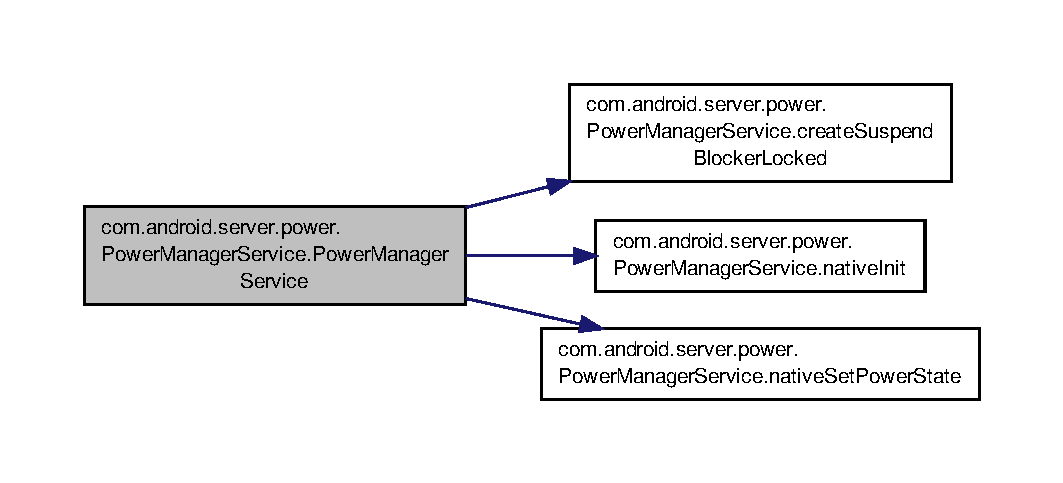
\includegraphics[width=350pt]{classcom_1_1android_1_1server_1_1power_1_1PowerManagerService_af61f43046957912e62237da840197b84_cgraph}
\end{center}
\end{figure}




\subsection{Member Function Documentation}
\hypertarget{classcom_1_1android_1_1server_1_1power_1_1PowerManagerService_a92faede593a057488165d627041ee2c2}{\index{com\-::android\-::server\-::power\-::\-Power\-Manager\-Service@{com\-::android\-::server\-::power\-::\-Power\-Manager\-Service}!acquire\-Htc\-Cpu\-Ctrl@{acquire\-Htc\-Cpu\-Ctrl}}
\index{acquire\-Htc\-Cpu\-Ctrl@{acquire\-Htc\-Cpu\-Ctrl}!com::android::server::power::PowerManagerService@{com\-::android\-::server\-::power\-::\-Power\-Manager\-Service}}
\subsubsection[{acquire\-Htc\-Cpu\-Ctrl}]{\setlength{\rightskip}{0pt plus 5cm}void com.\-android.\-server.\-power.\-Power\-Manager\-Service.\-acquire\-Htc\-Cpu\-Ctrl (
\begin{DoxyParamCaption}
\item[{int}]{flags, }
\item[{I\-Binder}]{lock, }
\item[{String}]{tag, }
\item[{Work\-Source}]{ws, }
\item[{int}]{level}
\end{DoxyParamCaption}
)\hspace{0.3cm}{\ttfamily [inline]}}}\label{classcom_1_1android_1_1server_1_1power_1_1PowerManagerService_a92faede593a057488165d627041ee2c2}


Here is the call graph for this function\-:
\nopagebreak
\begin{figure}[H]
\begin{center}
\leavevmode
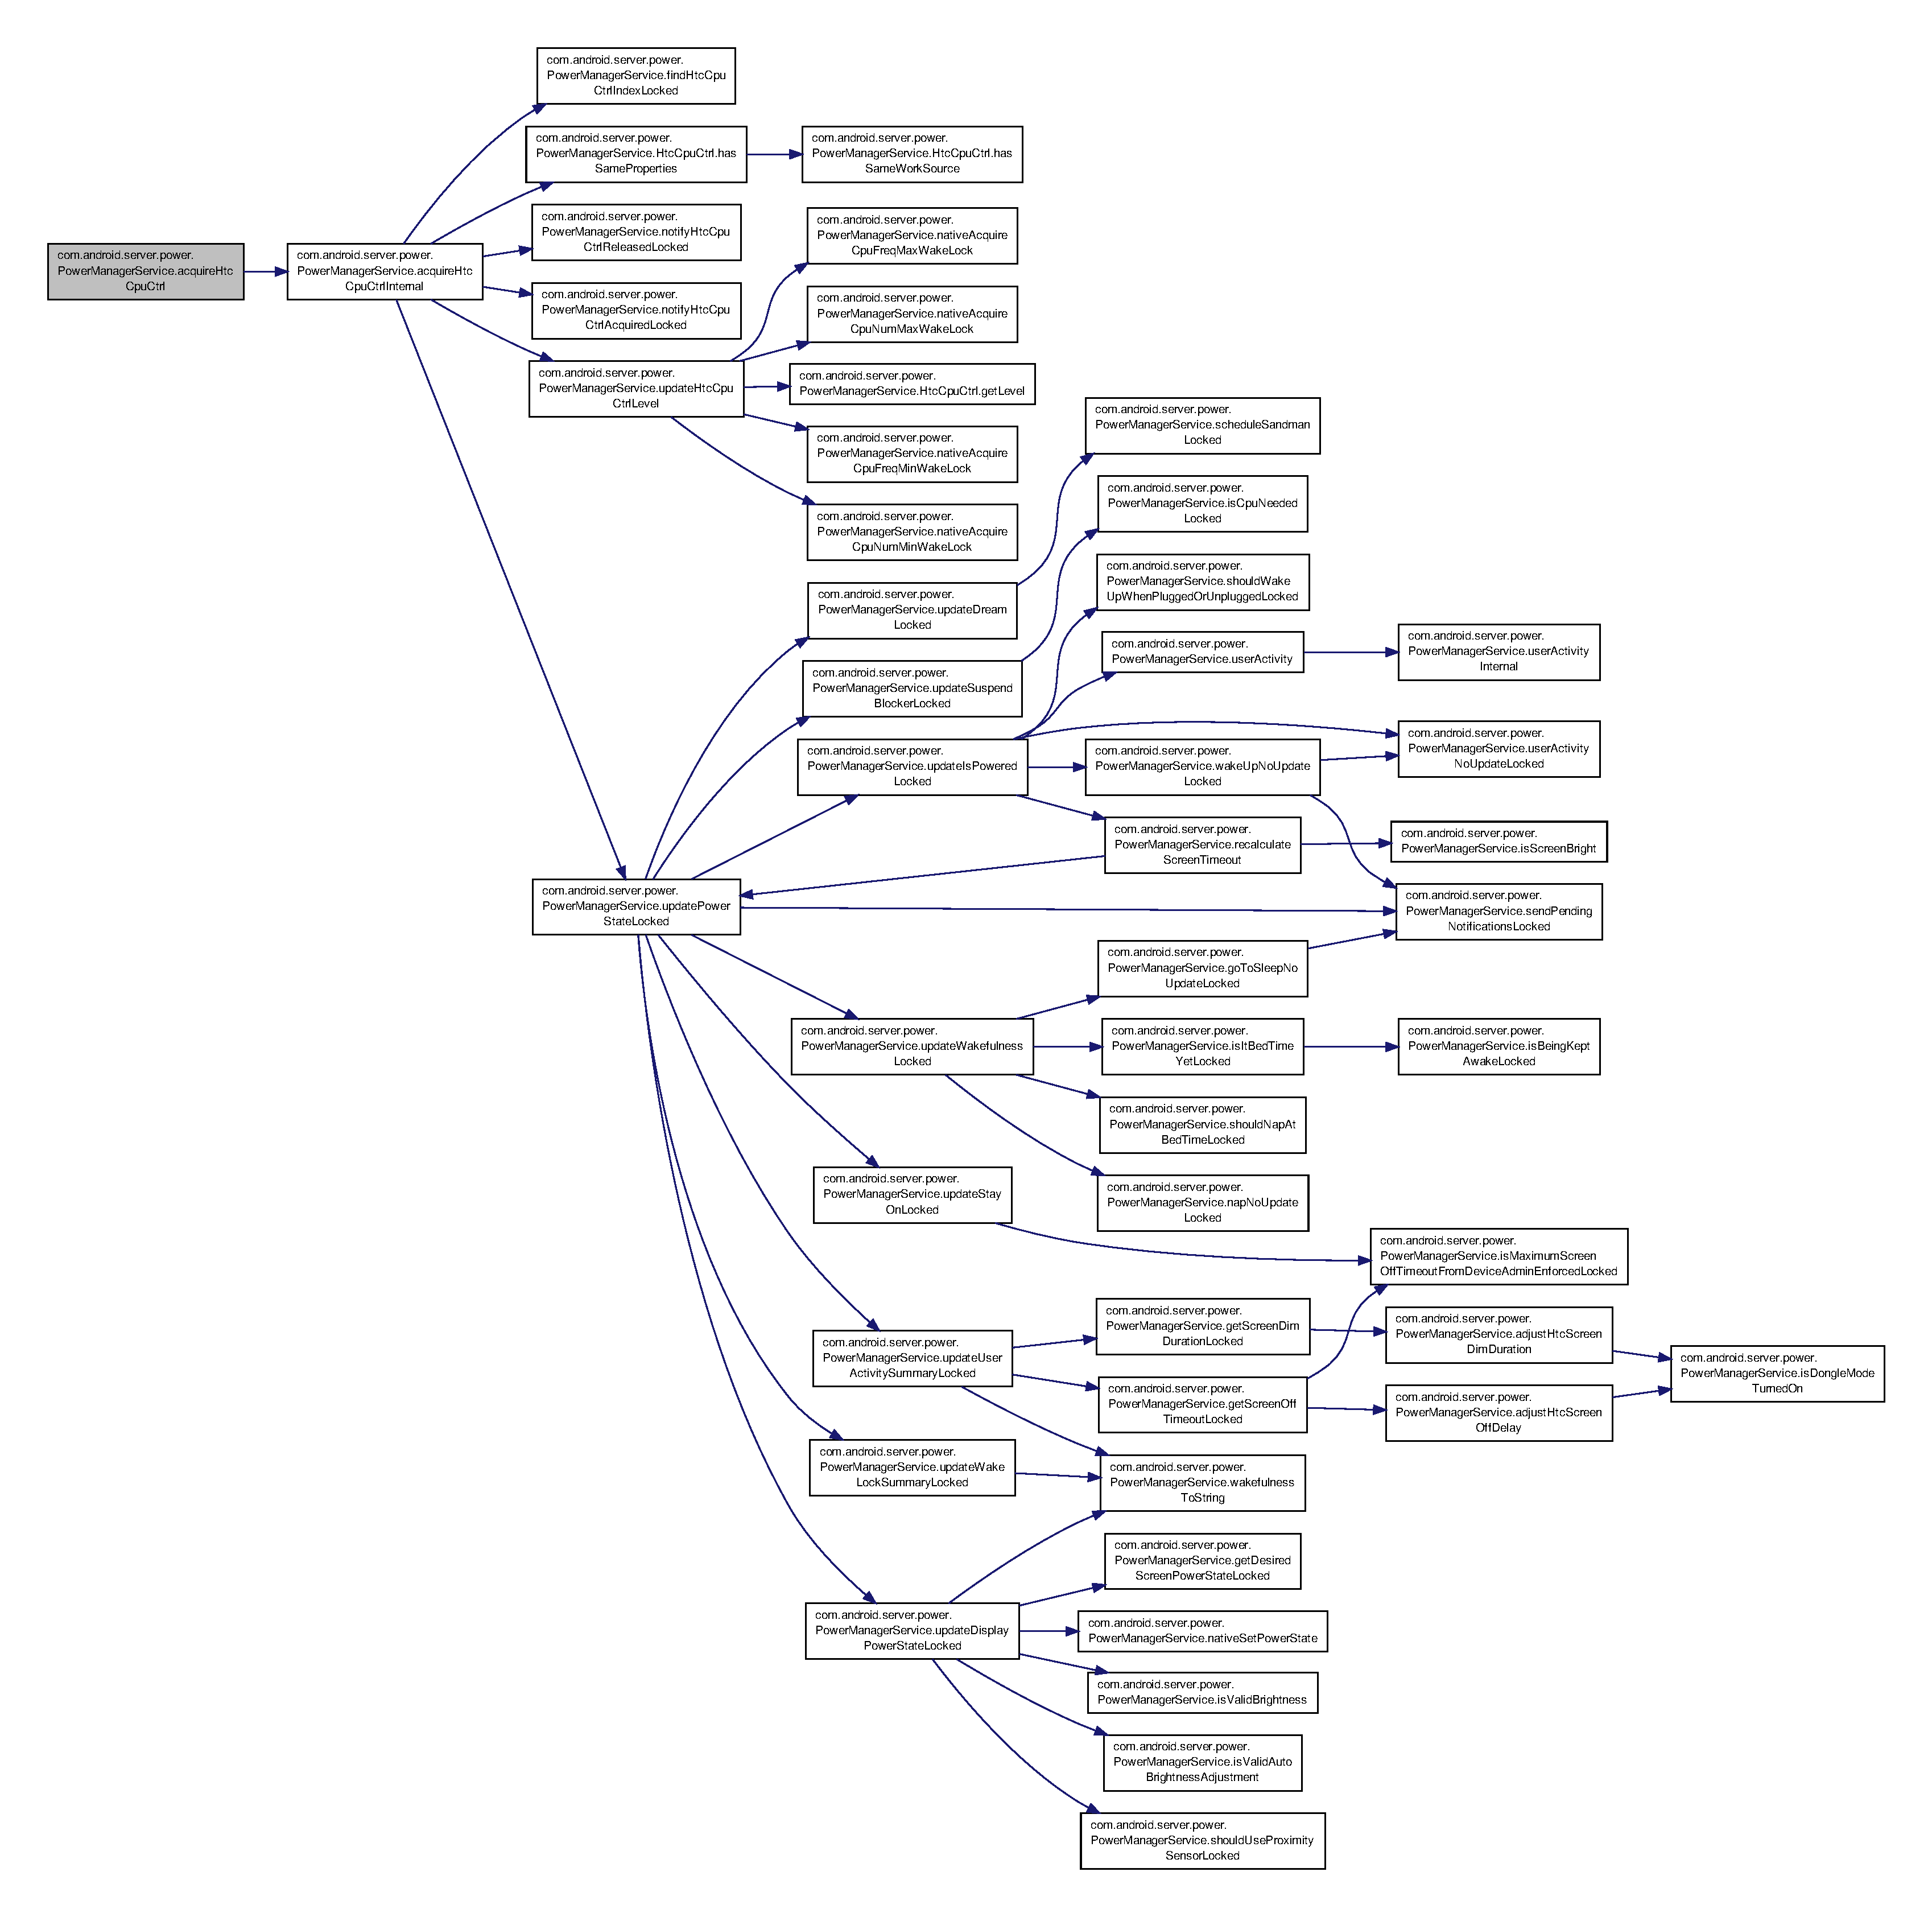
\includegraphics[width=350pt]{classcom_1_1android_1_1server_1_1power_1_1PowerManagerService_a92faede593a057488165d627041ee2c2_cgraph}
\end{center}
\end{figure}


\hypertarget{classcom_1_1android_1_1server_1_1power_1_1PowerManagerService_a322ee75df8e59595b7b35a8ee1a8d811}{\index{com\-::android\-::server\-::power\-::\-Power\-Manager\-Service@{com\-::android\-::server\-::power\-::\-Power\-Manager\-Service}!acquire\-Htc\-Cpu\-Ctrl\-Internal@{acquire\-Htc\-Cpu\-Ctrl\-Internal}}
\index{acquire\-Htc\-Cpu\-Ctrl\-Internal@{acquire\-Htc\-Cpu\-Ctrl\-Internal}!com::android::server::power::PowerManagerService@{com\-::android\-::server\-::power\-::\-Power\-Manager\-Service}}
\subsubsection[{acquire\-Htc\-Cpu\-Ctrl\-Internal}]{\setlength{\rightskip}{0pt plus 5cm}void com.\-android.\-server.\-power.\-Power\-Manager\-Service.\-acquire\-Htc\-Cpu\-Ctrl\-Internal (
\begin{DoxyParamCaption}
\item[{I\-Binder}]{lock, }
\item[{int}]{flags, }
\item[{String}]{tag, }
\item[{Work\-Source}]{ws, }
\item[{int}]{uid, }
\item[{int}]{pid, }
\item[{int}]{level}
\end{DoxyParamCaption}
)\hspace{0.3cm}{\ttfamily [inline]}, {\ttfamily [private]}}}\label{classcom_1_1android_1_1server_1_1power_1_1PowerManagerService_a322ee75df8e59595b7b35a8ee1a8d811}


Here is the call graph for this function\-:
\nopagebreak
\begin{figure}[H]
\begin{center}
\leavevmode
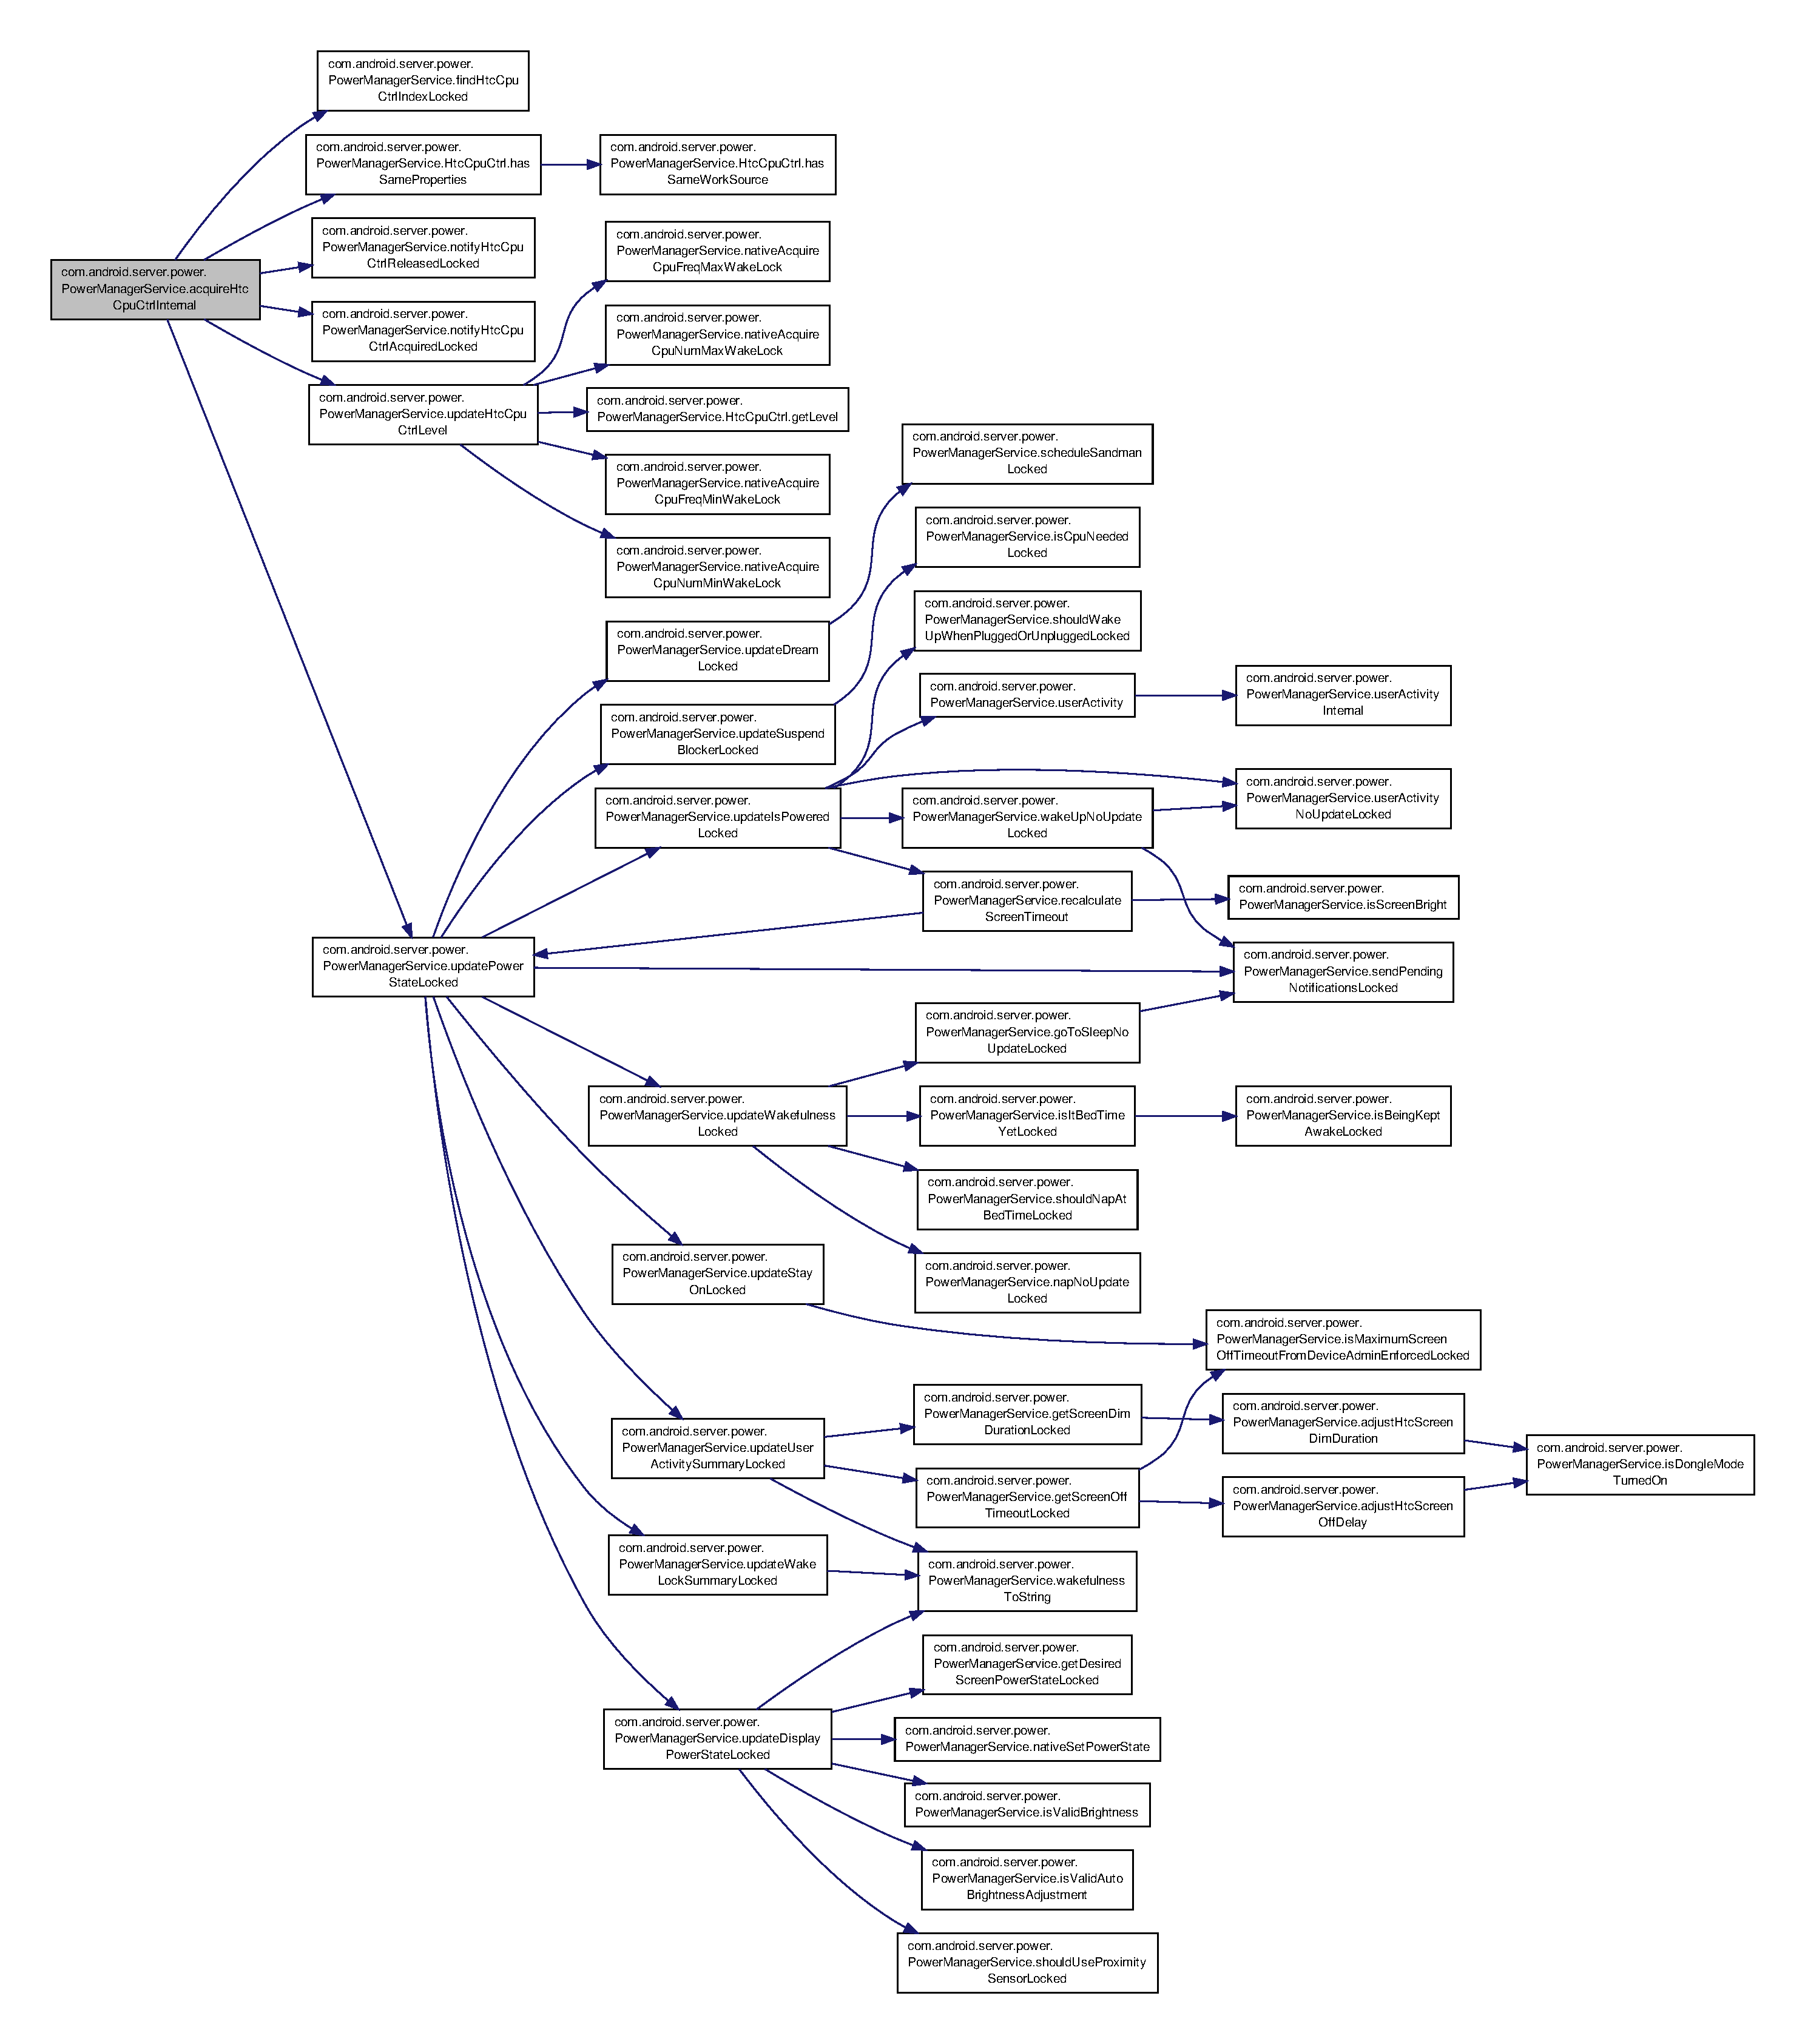
\includegraphics[width=350pt]{classcom_1_1android_1_1server_1_1power_1_1PowerManagerService_a322ee75df8e59595b7b35a8ee1a8d811_cgraph}
\end{center}
\end{figure}


\hypertarget{classcom_1_1android_1_1server_1_1power_1_1PowerManagerService_afeb6fabbab5aed353735777a05becf3f}{\index{com\-::android\-::server\-::power\-::\-Power\-Manager\-Service@{com\-::android\-::server\-::power\-::\-Power\-Manager\-Service}!acquire\-Wake\-Lock@{acquire\-Wake\-Lock}}
\index{acquire\-Wake\-Lock@{acquire\-Wake\-Lock}!com::android::server::power::PowerManagerService@{com\-::android\-::server\-::power\-::\-Power\-Manager\-Service}}
\subsubsection[{acquire\-Wake\-Lock}]{\setlength{\rightskip}{0pt plus 5cm}void com.\-android.\-server.\-power.\-Power\-Manager\-Service.\-acquire\-Wake\-Lock (
\begin{DoxyParamCaption}
\item[{I\-Binder}]{lock, }
\item[{int}]{flags, }
\item[{String}]{tag, }
\item[{Work\-Source}]{ws}
\end{DoxyParamCaption}
)\hspace{0.3cm}{\ttfamily [inline]}}}\label{classcom_1_1android_1_1server_1_1power_1_1PowerManagerService_afeb6fabbab5aed353735777a05becf3f}


Here is the call graph for this function\-:
\nopagebreak
\begin{figure}[H]
\begin{center}
\leavevmode
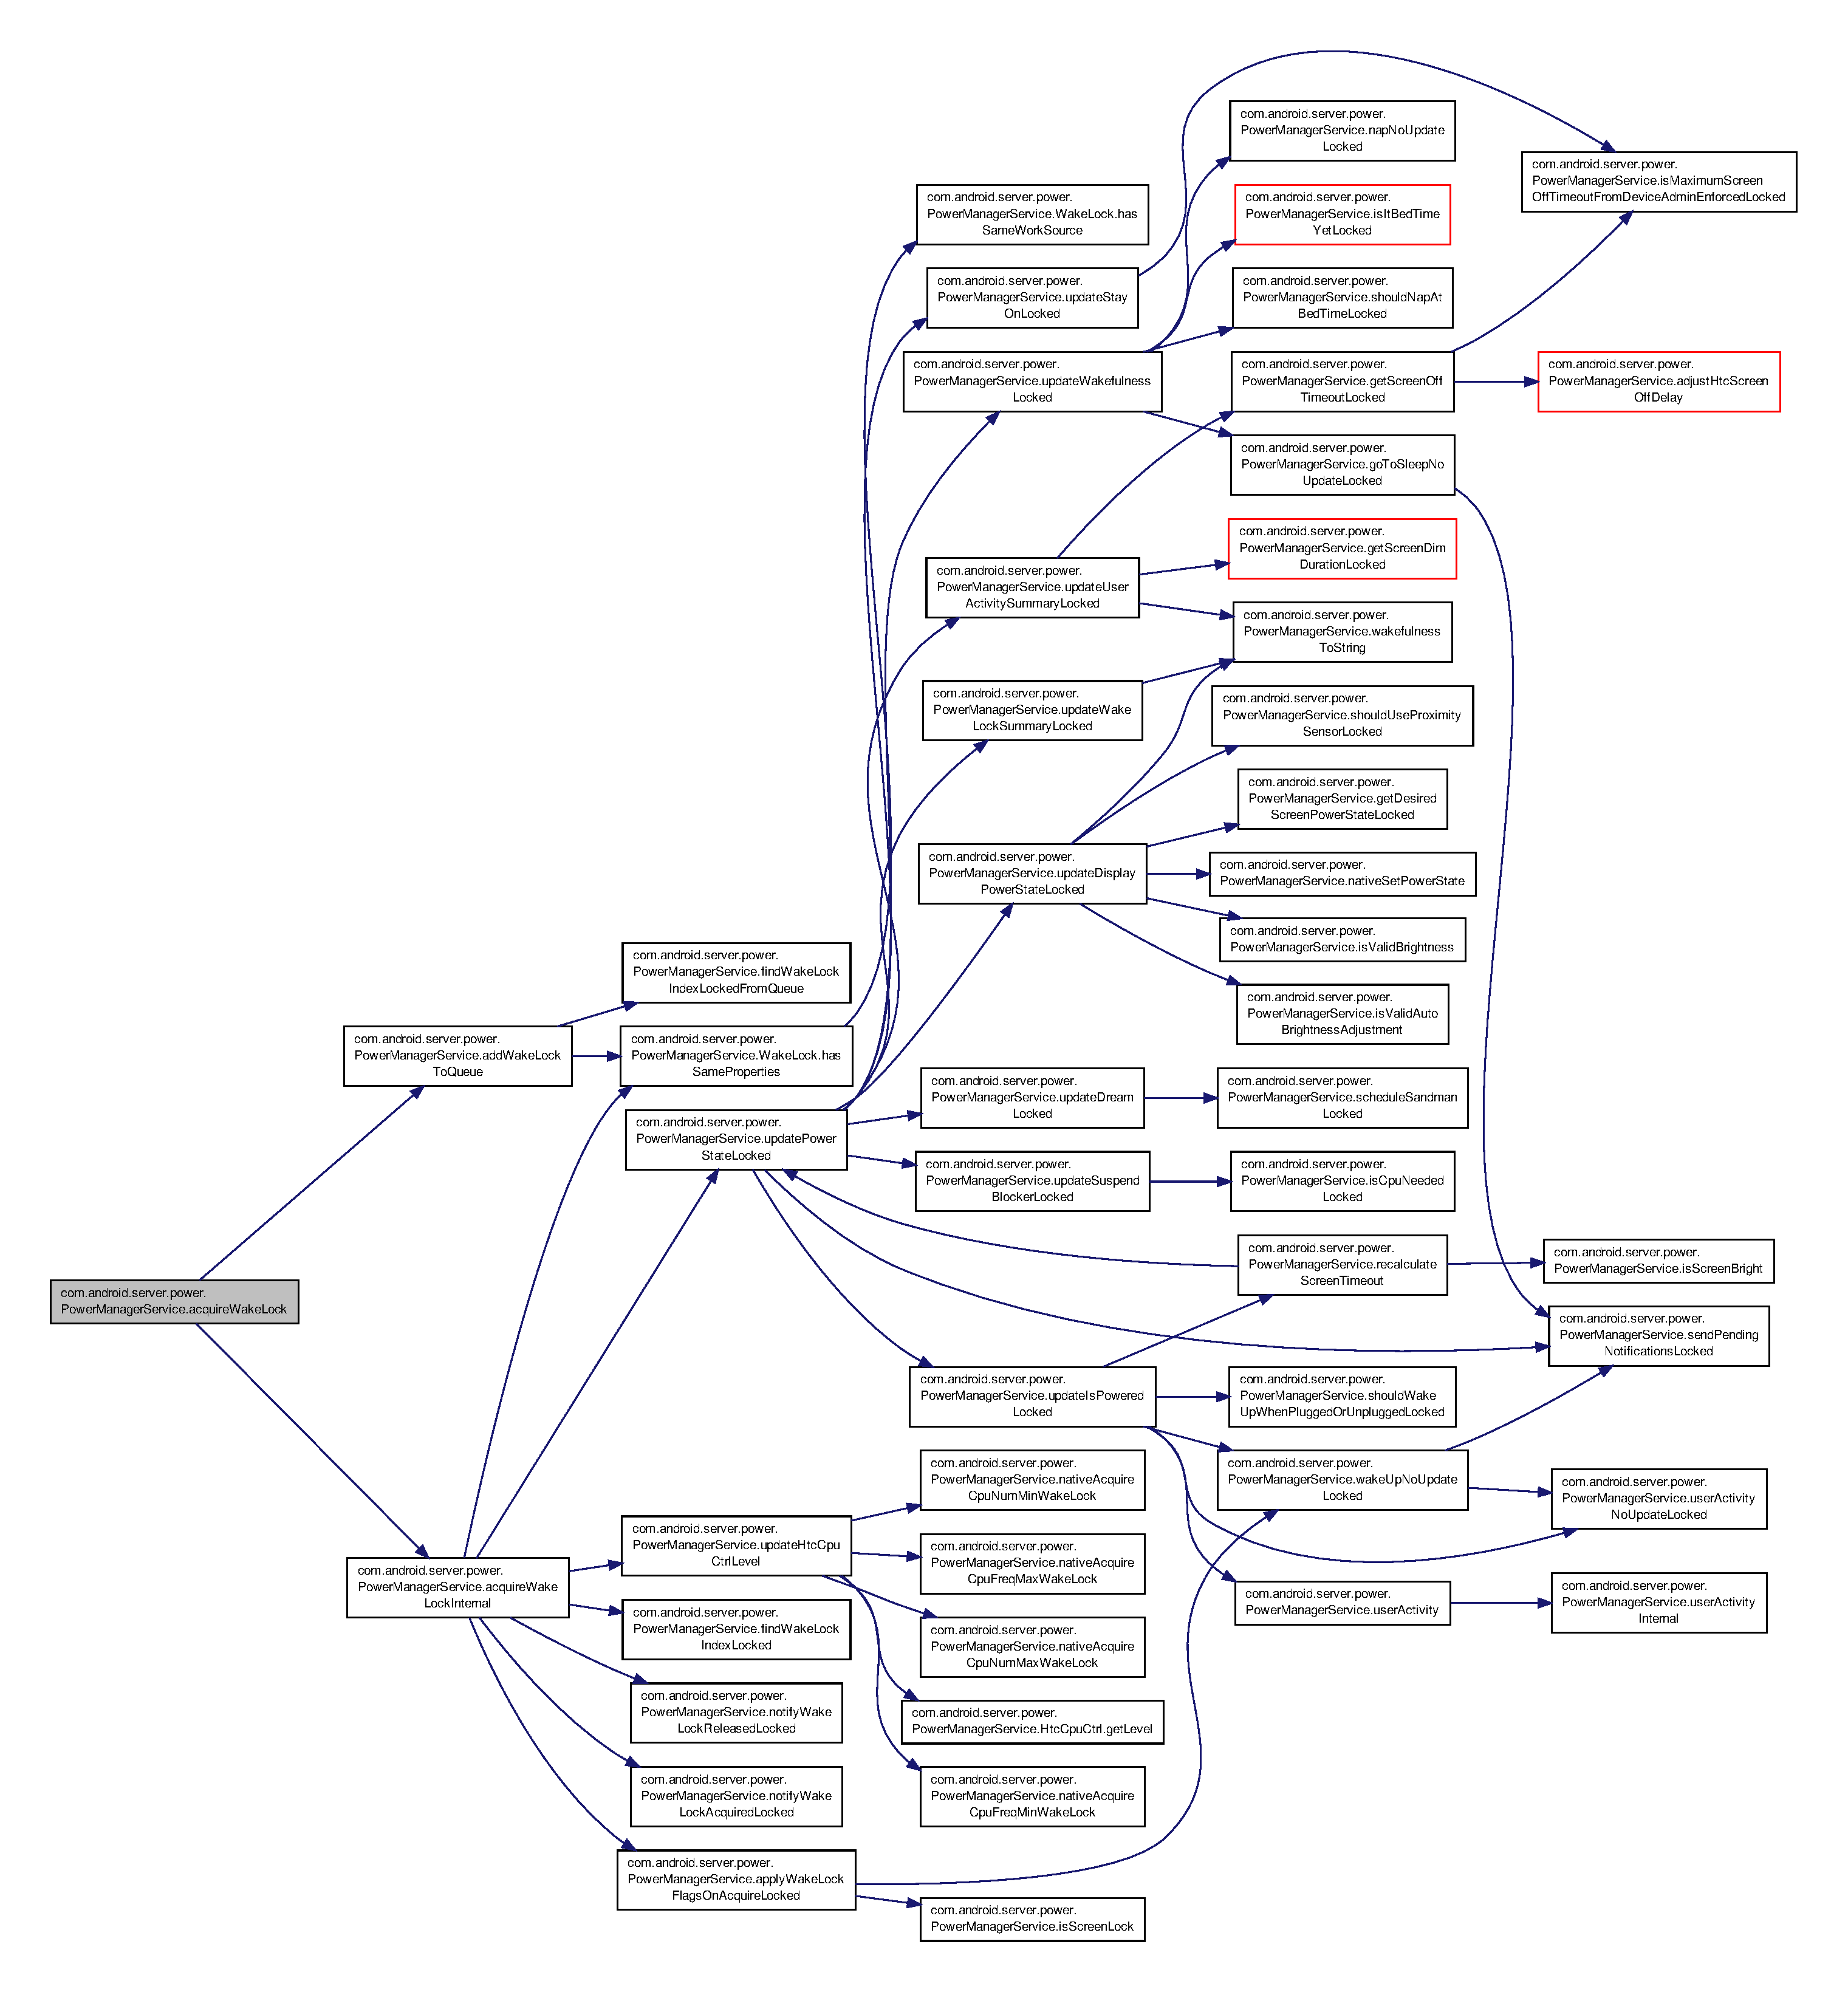
\includegraphics[width=350pt]{classcom_1_1android_1_1server_1_1power_1_1PowerManagerService_afeb6fabbab5aed353735777a05becf3f_cgraph}
\end{center}
\end{figure}


\hypertarget{classcom_1_1android_1_1server_1_1power_1_1PowerManagerService_a8062a7568b471234a9b21f700d9d1359}{\index{com\-::android\-::server\-::power\-::\-Power\-Manager\-Service@{com\-::android\-::server\-::power\-::\-Power\-Manager\-Service}!acquire\-Wake\-Lock\-Internal@{acquire\-Wake\-Lock\-Internal}}
\index{acquire\-Wake\-Lock\-Internal@{acquire\-Wake\-Lock\-Internal}!com::android::server::power::PowerManagerService@{com\-::android\-::server\-::power\-::\-Power\-Manager\-Service}}
\subsubsection[{acquire\-Wake\-Lock\-Internal}]{\setlength{\rightskip}{0pt plus 5cm}void com.\-android.\-server.\-power.\-Power\-Manager\-Service.\-acquire\-Wake\-Lock\-Internal (
\begin{DoxyParamCaption}
\item[{I\-Binder}]{lock, }
\item[{int}]{flags, }
\item[{String}]{tag, }
\item[{Work\-Source}]{ws, }
\item[{int}]{uid, }
\item[{int}]{pid}
\end{DoxyParamCaption}
)\hspace{0.3cm}{\ttfamily [inline]}, {\ttfamily [private]}}}\label{classcom_1_1android_1_1server_1_1power_1_1PowerManagerService_a8062a7568b471234a9b21f700d9d1359}


Here is the call graph for this function\-:
\nopagebreak
\begin{figure}[H]
\begin{center}
\leavevmode
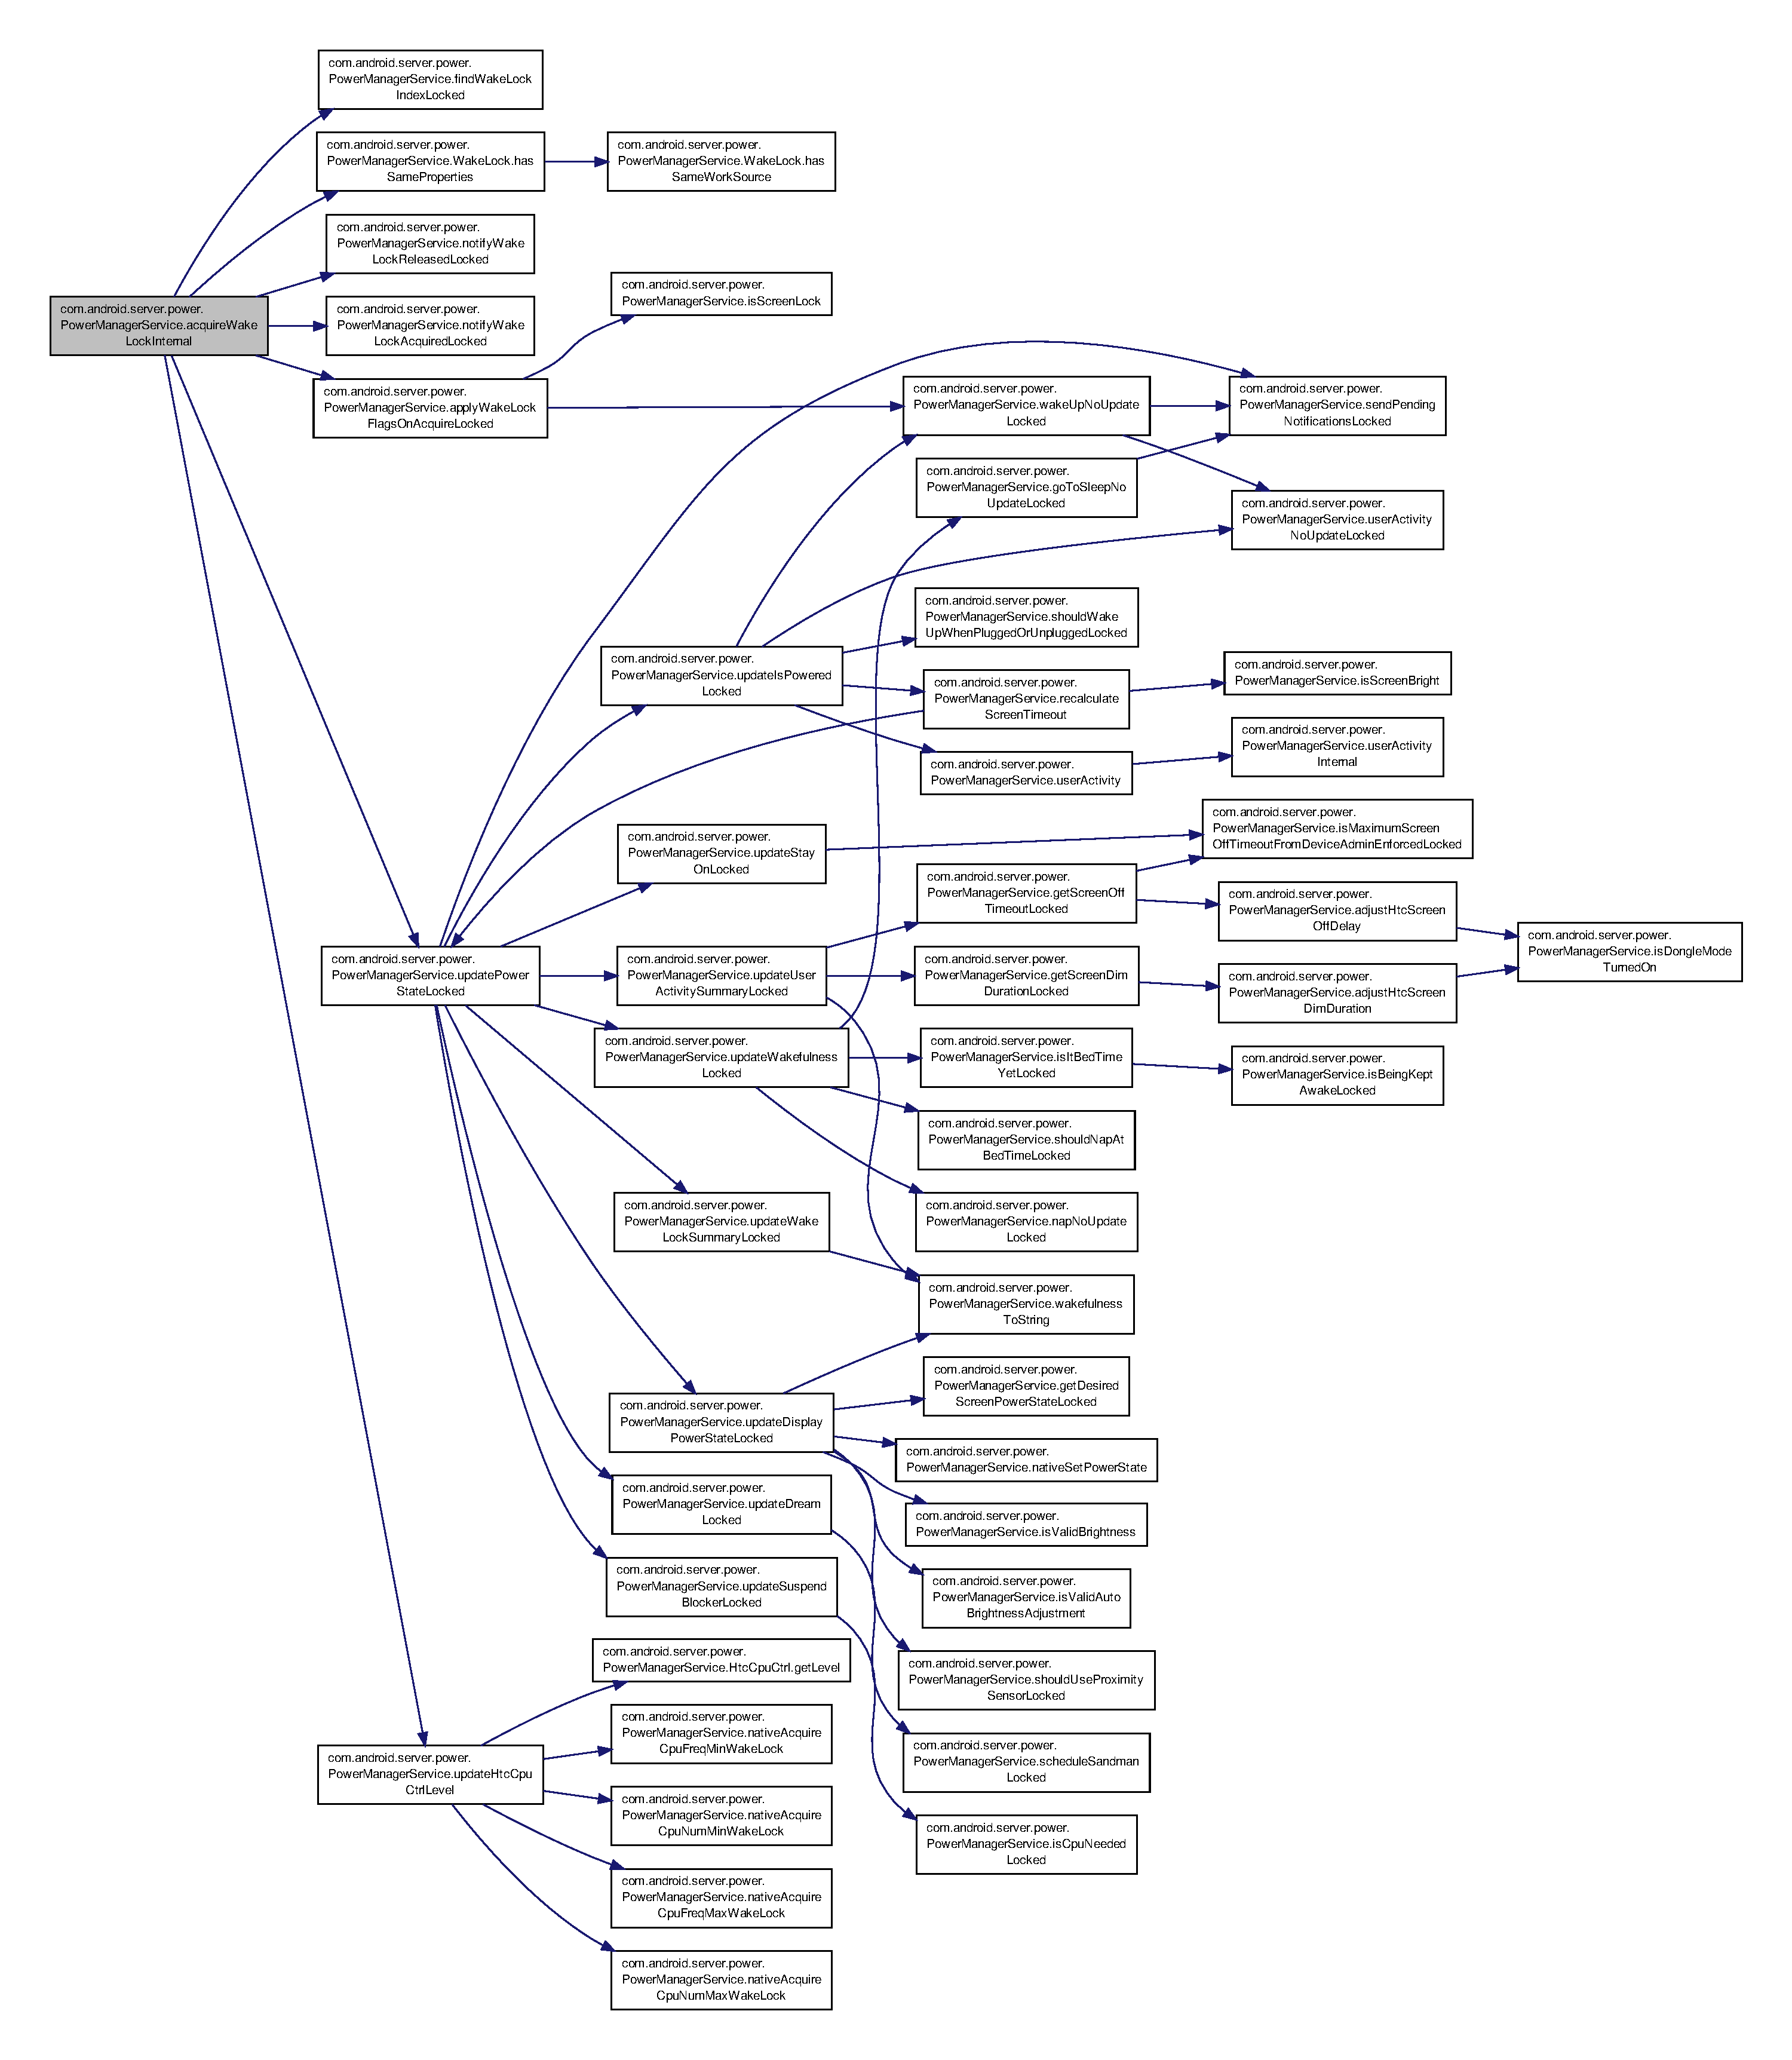
\includegraphics[width=350pt]{classcom_1_1android_1_1server_1_1power_1_1PowerManagerService_a8062a7568b471234a9b21f700d9d1359_cgraph}
\end{center}
\end{figure}


\hypertarget{classcom_1_1android_1_1server_1_1power_1_1PowerManagerService_a07c4777bfd8a6f3cb3adb843277165d5}{\index{com\-::android\-::server\-::power\-::\-Power\-Manager\-Service@{com\-::android\-::server\-::power\-::\-Power\-Manager\-Service}!add\-Wake\-Lock\-To\-Queue@{add\-Wake\-Lock\-To\-Queue}}
\index{add\-Wake\-Lock\-To\-Queue@{add\-Wake\-Lock\-To\-Queue}!com::android::server::power::PowerManagerService@{com\-::android\-::server\-::power\-::\-Power\-Manager\-Service}}
\subsubsection[{add\-Wake\-Lock\-To\-Queue}]{\setlength{\rightskip}{0pt plus 5cm}void com.\-android.\-server.\-power.\-Power\-Manager\-Service.\-add\-Wake\-Lock\-To\-Queue (
\begin{DoxyParamCaption}
\item[{I\-Binder}]{lock, }
\item[{int}]{flags, }
\item[{String}]{tag, }
\item[{Work\-Source}]{ws, }
\item[{int}]{uid, }
\item[{int}]{pid}
\end{DoxyParamCaption}
)\hspace{0.3cm}{\ttfamily [inline]}, {\ttfamily [private]}}}\label{classcom_1_1android_1_1server_1_1power_1_1PowerManagerService_a07c4777bfd8a6f3cb3adb843277165d5}


Here is the call graph for this function\-:
\nopagebreak
\begin{figure}[H]
\begin{center}
\leavevmode
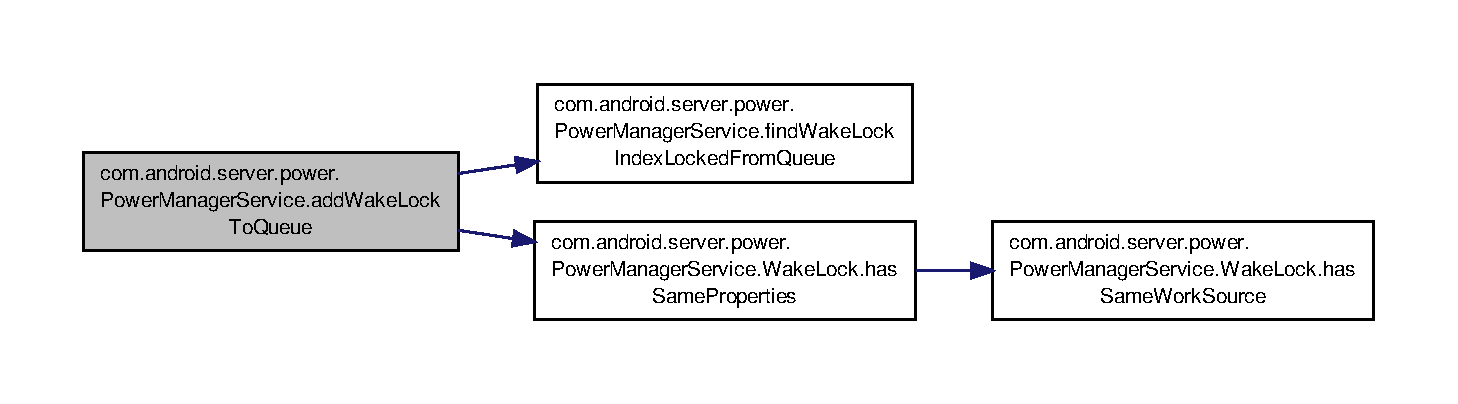
\includegraphics[width=350pt]{classcom_1_1android_1_1server_1_1power_1_1PowerManagerService_a07c4777bfd8a6f3cb3adb843277165d5_cgraph}
\end{center}
\end{figure}


\hypertarget{classcom_1_1android_1_1server_1_1power_1_1PowerManagerService_a37c5f253d91125be9c855be7a777950f}{\index{com\-::android\-::server\-::power\-::\-Power\-Manager\-Service@{com\-::android\-::server\-::power\-::\-Power\-Manager\-Service}!adjust\-Htc\-Screen\-Dim\-Duration@{adjust\-Htc\-Screen\-Dim\-Duration}}
\index{adjust\-Htc\-Screen\-Dim\-Duration@{adjust\-Htc\-Screen\-Dim\-Duration}!com::android::server::power::PowerManagerService@{com\-::android\-::server\-::power\-::\-Power\-Manager\-Service}}
\subsubsection[{adjust\-Htc\-Screen\-Dim\-Duration}]{\setlength{\rightskip}{0pt plus 5cm}int com.\-android.\-server.\-power.\-Power\-Manager\-Service.\-adjust\-Htc\-Screen\-Dim\-Duration (
\begin{DoxyParamCaption}
\item[{final int}]{screen\-Off\-Timeout}
\end{DoxyParamCaption}
)\hspace{0.3cm}{\ttfamily [inline]}, {\ttfamily [private]}}}\label{classcom_1_1android_1_1server_1_1power_1_1PowerManagerService_a37c5f253d91125be9c855be7a777950f}


Here is the call graph for this function\-:
\nopagebreak
\begin{figure}[H]
\begin{center}
\leavevmode
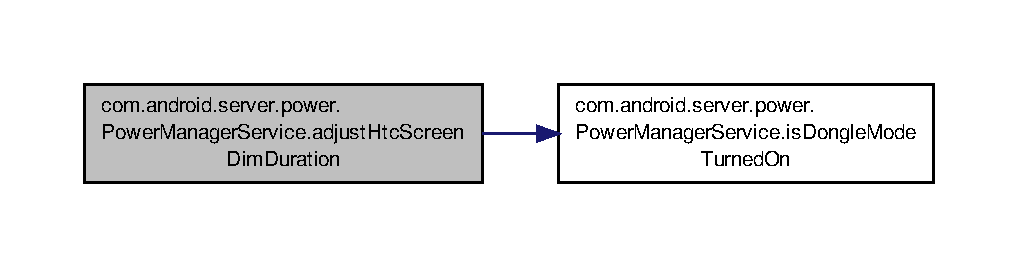
\includegraphics[width=350pt]{classcom_1_1android_1_1server_1_1power_1_1PowerManagerService_a37c5f253d91125be9c855be7a777950f_cgraph}
\end{center}
\end{figure}


\hypertarget{classcom_1_1android_1_1server_1_1power_1_1PowerManagerService_a6b6d93b9189fc73e7e1e3fd8e71238b6}{\index{com\-::android\-::server\-::power\-::\-Power\-Manager\-Service@{com\-::android\-::server\-::power\-::\-Power\-Manager\-Service}!adjust\-Htc\-Screen\-Off\-Delay@{adjust\-Htc\-Screen\-Off\-Delay}}
\index{adjust\-Htc\-Screen\-Off\-Delay@{adjust\-Htc\-Screen\-Off\-Delay}!com::android::server::power::PowerManagerService@{com\-::android\-::server\-::power\-::\-Power\-Manager\-Service}}
\subsubsection[{adjust\-Htc\-Screen\-Off\-Delay}]{\setlength{\rightskip}{0pt plus 5cm}int com.\-android.\-server.\-power.\-Power\-Manager\-Service.\-adjust\-Htc\-Screen\-Off\-Delay (
\begin{DoxyParamCaption}
\item[{int}]{total\-Delay}
\end{DoxyParamCaption}
)\hspace{0.3cm}{\ttfamily [inline]}, {\ttfamily [private]}}}\label{classcom_1_1android_1_1server_1_1power_1_1PowerManagerService_a6b6d93b9189fc73e7e1e3fd8e71238b6}


Here is the call graph for this function\-:
\nopagebreak
\begin{figure}[H]
\begin{center}
\leavevmode
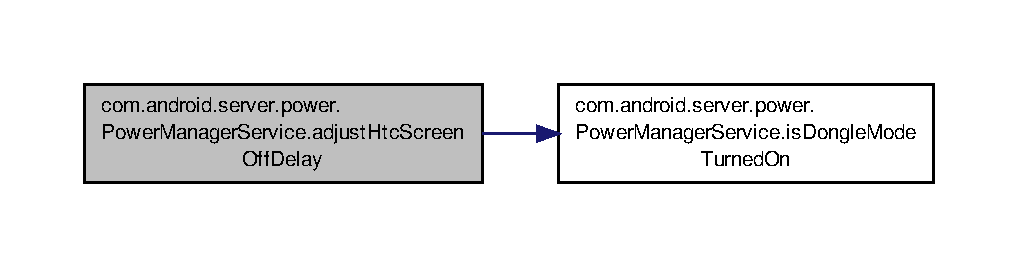
\includegraphics[width=350pt]{classcom_1_1android_1_1server_1_1power_1_1PowerManagerService_a6b6d93b9189fc73e7e1e3fd8e71238b6_cgraph}
\end{center}
\end{figure}


\hypertarget{classcom_1_1android_1_1server_1_1power_1_1PowerManagerService_a95099e0f6140722c01006bd184b74179}{\index{com\-::android\-::server\-::power\-::\-Power\-Manager\-Service@{com\-::android\-::server\-::power\-::\-Power\-Manager\-Service}!apply\-Wake\-Lock\-Flags\-On\-Acquire\-Locked@{apply\-Wake\-Lock\-Flags\-On\-Acquire\-Locked}}
\index{apply\-Wake\-Lock\-Flags\-On\-Acquire\-Locked@{apply\-Wake\-Lock\-Flags\-On\-Acquire\-Locked}!com::android::server::power::PowerManagerService@{com\-::android\-::server\-::power\-::\-Power\-Manager\-Service}}
\subsubsection[{apply\-Wake\-Lock\-Flags\-On\-Acquire\-Locked}]{\setlength{\rightskip}{0pt plus 5cm}void com.\-android.\-server.\-power.\-Power\-Manager\-Service.\-apply\-Wake\-Lock\-Flags\-On\-Acquire\-Locked (
\begin{DoxyParamCaption}
\item[{{\bf Wake\-Lock}}]{wake\-Lock}
\end{DoxyParamCaption}
)\hspace{0.3cm}{\ttfamily [inline]}, {\ttfamily [private]}}}\label{classcom_1_1android_1_1server_1_1power_1_1PowerManagerService_a95099e0f6140722c01006bd184b74179}


Here is the call graph for this function\-:
\nopagebreak
\begin{figure}[H]
\begin{center}
\leavevmode
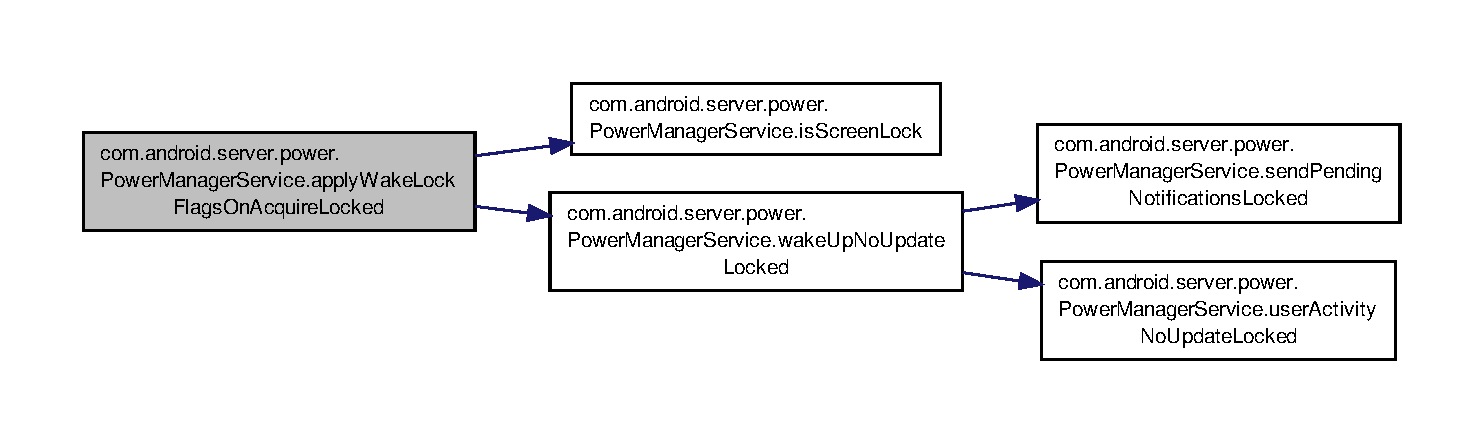
\includegraphics[width=350pt]{classcom_1_1android_1_1server_1_1power_1_1PowerManagerService_a95099e0f6140722c01006bd184b74179_cgraph}
\end{center}
\end{figure}


\hypertarget{classcom_1_1android_1_1server_1_1power_1_1PowerManagerService_a6fd027d7c3d94f880afcde5f3fc67b0a}{\index{com\-::android\-::server\-::power\-::\-Power\-Manager\-Service@{com\-::android\-::server\-::power\-::\-Power\-Manager\-Service}!apply\-Wake\-Lock\-Flags\-On\-Release\-Locked@{apply\-Wake\-Lock\-Flags\-On\-Release\-Locked}}
\index{apply\-Wake\-Lock\-Flags\-On\-Release\-Locked@{apply\-Wake\-Lock\-Flags\-On\-Release\-Locked}!com::android::server::power::PowerManagerService@{com\-::android\-::server\-::power\-::\-Power\-Manager\-Service}}
\subsubsection[{apply\-Wake\-Lock\-Flags\-On\-Release\-Locked}]{\setlength{\rightskip}{0pt plus 5cm}void com.\-android.\-server.\-power.\-Power\-Manager\-Service.\-apply\-Wake\-Lock\-Flags\-On\-Release\-Locked (
\begin{DoxyParamCaption}
\item[{{\bf Wake\-Lock}}]{wake\-Lock}
\end{DoxyParamCaption}
)\hspace{0.3cm}{\ttfamily [inline]}, {\ttfamily [private]}}}\label{classcom_1_1android_1_1server_1_1power_1_1PowerManagerService_a6fd027d7c3d94f880afcde5f3fc67b0a}


Here is the call graph for this function\-:
\nopagebreak
\begin{figure}[H]
\begin{center}
\leavevmode
\includegraphics[width=350pt]{classcom_1_1android_1_1server_1_1power_1_1PowerManagerService_a6fd027d7c3d94f880afcde5f3fc67b0a_cgraph}
\end{center}
\end{figure}


\hypertarget{classcom_1_1android_1_1server_1_1power_1_1PowerManagerService_ae9ad75267601483cdd11f47940a15af1}{\index{com\-::android\-::server\-::power\-::\-Power\-Manager\-Service@{com\-::android\-::server\-::power\-::\-Power\-Manager\-Service}!can\-Dream\-Locked@{can\-Dream\-Locked}}
\index{can\-Dream\-Locked@{can\-Dream\-Locked}!com::android::server::power::PowerManagerService@{com\-::android\-::server\-::power\-::\-Power\-Manager\-Service}}
\subsubsection[{can\-Dream\-Locked}]{\setlength{\rightskip}{0pt plus 5cm}boolean com.\-android.\-server.\-power.\-Power\-Manager\-Service.\-can\-Dream\-Locked (
\begin{DoxyParamCaption}
{}
\end{DoxyParamCaption}
)\hspace{0.3cm}{\ttfamily [inline]}, {\ttfamily [private]}}}\label{classcom_1_1android_1_1server_1_1power_1_1PowerManagerService_ae9ad75267601483cdd11f47940a15af1}
Returns true if the device is allowed to dream in its current state assuming that it is currently napping or dreaming. 

Here is the call graph for this function\-:
\nopagebreak
\begin{figure}[H]
\begin{center}
\leavevmode
\includegraphics[width=350pt]{classcom_1_1android_1_1server_1_1power_1_1PowerManagerService_ae9ad75267601483cdd11f47940a15af1_cgraph}
\end{center}
\end{figure}


\hypertarget{classcom_1_1android_1_1server_1_1power_1_1PowerManagerService_a6e6bee2d07f48c66f5eddb6247bce35a}{\index{com\-::android\-::server\-::power\-::\-Power\-Manager\-Service@{com\-::android\-::server\-::power\-::\-Power\-Manager\-Service}!check\-If\-Boot\-Animation\-Finished@{check\-If\-Boot\-Animation\-Finished}}
\index{check\-If\-Boot\-Animation\-Finished@{check\-If\-Boot\-Animation\-Finished}!com::android::server::power::PowerManagerService@{com\-::android\-::server\-::power\-::\-Power\-Manager\-Service}}
\subsubsection[{check\-If\-Boot\-Animation\-Finished}]{\setlength{\rightskip}{0pt plus 5cm}void com.\-android.\-server.\-power.\-Power\-Manager\-Service.\-check\-If\-Boot\-Animation\-Finished (
\begin{DoxyParamCaption}
{}
\end{DoxyParamCaption}
)\hspace{0.3cm}{\ttfamily [inline]}, {\ttfamily [private]}}}\label{classcom_1_1android_1_1server_1_1power_1_1PowerManagerService_a6e6bee2d07f48c66f5eddb6247bce35a}


Here is the call graph for this function\-:
\nopagebreak
\begin{figure}[H]
\begin{center}
\leavevmode
\includegraphics[width=350pt]{classcom_1_1android_1_1server_1_1power_1_1PowerManagerService_a6e6bee2d07f48c66f5eddb6247bce35a_cgraph}
\end{center}
\end{figure}


\hypertarget{classcom_1_1android_1_1server_1_1power_1_1PowerManagerService_a01870610adf1bddff8377ead48478964}{\index{com\-::android\-::server\-::power\-::\-Power\-Manager\-Service@{com\-::android\-::server\-::power\-::\-Power\-Manager\-Service}!check\-If\-O\-O\-B\-E\-Status\-Finished@{check\-If\-O\-O\-B\-E\-Status\-Finished}}
\index{check\-If\-O\-O\-B\-E\-Status\-Finished@{check\-If\-O\-O\-B\-E\-Status\-Finished}!com::android::server::power::PowerManagerService@{com\-::android\-::server\-::power\-::\-Power\-Manager\-Service}}
\subsubsection[{check\-If\-O\-O\-B\-E\-Status\-Finished}]{\setlength{\rightskip}{0pt plus 5cm}boolean com.\-android.\-server.\-power.\-Power\-Manager\-Service.\-check\-If\-O\-O\-B\-E\-Status\-Finished (
\begin{DoxyParamCaption}
\item[{boolean}]{is\-Timeout}
\end{DoxyParamCaption}
)\hspace{0.3cm}{\ttfamily [inline]}, {\ttfamily [private]}}}\label{classcom_1_1android_1_1server_1_1power_1_1PowerManagerService_a01870610adf1bddff8377ead48478964}
\hypertarget{classcom_1_1android_1_1server_1_1power_1_1PowerManagerService_a864904faf25924bfc3b6c5b268836741}{\index{com\-::android\-::server\-::power\-::\-Power\-Manager\-Service@{com\-::android\-::server\-::power\-::\-Power\-Manager\-Service}!clear\-Monitor\-O\-O\-B\-E\-Status@{clear\-Monitor\-O\-O\-B\-E\-Status}}
\index{clear\-Monitor\-O\-O\-B\-E\-Status@{clear\-Monitor\-O\-O\-B\-E\-Status}!com::android::server::power::PowerManagerService@{com\-::android\-::server\-::power\-::\-Power\-Manager\-Service}}
\subsubsection[{clear\-Monitor\-O\-O\-B\-E\-Status}]{\setlength{\rightskip}{0pt plus 5cm}void com.\-android.\-server.\-power.\-Power\-Manager\-Service.\-clear\-Monitor\-O\-O\-B\-E\-Status (
\begin{DoxyParamCaption}
{}
\end{DoxyParamCaption}
)\hspace{0.3cm}{\ttfamily [inline]}, {\ttfamily [private]}}}\label{classcom_1_1android_1_1server_1_1power_1_1PowerManagerService_a864904faf25924bfc3b6c5b268836741}
\hypertarget{classcom_1_1android_1_1server_1_1power_1_1PowerManagerService_a34fbb15121aaebb932695dcb81511734}{\index{com\-::android\-::server\-::power\-::\-Power\-Manager\-Service@{com\-::android\-::server\-::power\-::\-Power\-Manager\-Service}!copy\-Work\-Source@{copy\-Work\-Source}}
\index{copy\-Work\-Source@{copy\-Work\-Source}!com::android::server::power::PowerManagerService@{com\-::android\-::server\-::power\-::\-Power\-Manager\-Service}}
\subsubsection[{copy\-Work\-Source}]{\setlength{\rightskip}{0pt plus 5cm}static Work\-Source com.\-android.\-server.\-power.\-Power\-Manager\-Service.\-copy\-Work\-Source (
\begin{DoxyParamCaption}
\item[{Work\-Source}]{work\-Source}
\end{DoxyParamCaption}
)\hspace{0.3cm}{\ttfamily [inline]}, {\ttfamily [static]}, {\ttfamily [private]}}}\label{classcom_1_1android_1_1server_1_1power_1_1PowerManagerService_a34fbb15121aaebb932695dcb81511734}
\hypertarget{classcom_1_1android_1_1server_1_1power_1_1PowerManagerService_a98ff223785ece7b9c30e8ecca67b7867}{\index{com\-::android\-::server\-::power\-::\-Power\-Manager\-Service@{com\-::android\-::server\-::power\-::\-Power\-Manager\-Service}!crash@{crash}}
\index{crash@{crash}!com::android::server::power::PowerManagerService@{com\-::android\-::server\-::power\-::\-Power\-Manager\-Service}}
\subsubsection[{crash}]{\setlength{\rightskip}{0pt plus 5cm}void com.\-android.\-server.\-power.\-Power\-Manager\-Service.\-crash (
\begin{DoxyParamCaption}
\item[{String}]{message}
\end{DoxyParamCaption}
)\hspace{0.3cm}{\ttfamily [inline]}}}\label{classcom_1_1android_1_1server_1_1power_1_1PowerManagerService_a98ff223785ece7b9c30e8ecca67b7867}
Crash the runtime (causing a complete restart of the Android framework). Requires R\-E\-B\-O\-O\-T permission. Mostly for testing. Should not return. 

Here is the call graph for this function\-:
\nopagebreak
\begin{figure}[H]
\begin{center}
\leavevmode
\includegraphics[width=350pt]{classcom_1_1android_1_1server_1_1power_1_1PowerManagerService_a98ff223785ece7b9c30e8ecca67b7867_cgraph}
\end{center}
\end{figure}


\hypertarget{classcom_1_1android_1_1server_1_1power_1_1PowerManagerService_ad1a8d7c25597561b2adc8d41913d31c8}{\index{com\-::android\-::server\-::power\-::\-Power\-Manager\-Service@{com\-::android\-::server\-::power\-::\-Power\-Manager\-Service}!crash\-Internal@{crash\-Internal}}
\index{crash\-Internal@{crash\-Internal}!com::android::server::power::PowerManagerService@{com\-::android\-::server\-::power\-::\-Power\-Manager\-Service}}
\subsubsection[{crash\-Internal}]{\setlength{\rightskip}{0pt plus 5cm}void com.\-android.\-server.\-power.\-Power\-Manager\-Service.\-crash\-Internal (
\begin{DoxyParamCaption}
\item[{final String}]{message}
\end{DoxyParamCaption}
)\hspace{0.3cm}{\ttfamily [inline]}, {\ttfamily [private]}}}\label{classcom_1_1android_1_1server_1_1power_1_1PowerManagerService_ad1a8d7c25597561b2adc8d41913d31c8}
\hypertarget{classcom_1_1android_1_1server_1_1power_1_1PowerManagerService_ab3b092c1dc0fafc3a799aa63190236c4}{\index{com\-::android\-::server\-::power\-::\-Power\-Manager\-Service@{com\-::android\-::server\-::power\-::\-Power\-Manager\-Service}!create\-Suspend\-Blocker\-Locked@{create\-Suspend\-Blocker\-Locked}}
\index{create\-Suspend\-Blocker\-Locked@{create\-Suspend\-Blocker\-Locked}!com::android::server::power::PowerManagerService@{com\-::android\-::server\-::power\-::\-Power\-Manager\-Service}}
\subsubsection[{create\-Suspend\-Blocker\-Locked}]{\setlength{\rightskip}{0pt plus 5cm}Suspend\-Blocker com.\-android.\-server.\-power.\-Power\-Manager\-Service.\-create\-Suspend\-Blocker\-Locked (
\begin{DoxyParamCaption}
\item[{String}]{name}
\end{DoxyParamCaption}
)\hspace{0.3cm}{\ttfamily [inline]}, {\ttfamily [private]}}}\label{classcom_1_1android_1_1server_1_1power_1_1PowerManagerService_ab3b092c1dc0fafc3a799aa63190236c4}
\hypertarget{classcom_1_1android_1_1server_1_1power_1_1PowerManagerService_aaee5f3f019a74b2bf1099b85a61758a8}{\index{com\-::android\-::server\-::power\-::\-Power\-Manager\-Service@{com\-::android\-::server\-::power\-::\-Power\-Manager\-Service}!customize\-Screen\-Off\-Delay\-\_\-\-Always@{customize\-Screen\-Off\-Delay\-\_\-\-Always}}
\index{customize\-Screen\-Off\-Delay\-\_\-\-Always@{customize\-Screen\-Off\-Delay\-\_\-\-Always}!com::android::server::power::PowerManagerService@{com\-::android\-::server\-::power\-::\-Power\-Manager\-Service}}
\subsubsection[{customize\-Screen\-Off\-Delay\-\_\-\-Always}]{\setlength{\rightskip}{0pt plus 5cm}void com.\-android.\-server.\-power.\-Power\-Manager\-Service.\-customize\-Screen\-Off\-Delay\-\_\-\-Always (
\begin{DoxyParamCaption}
\item[{final int}]{screen\-Off\-Delay, }
\item[{final boolean}]{calc\-Remaining}
\end{DoxyParamCaption}
)\hspace{0.3cm}{\ttfamily [inline]}}}\label{classcom_1_1android_1_1server_1_1power_1_1PowerManagerService_aaee5f3f019a74b2bf1099b85a61758a8}


Here is the call graph for this function\-:
\nopagebreak
\begin{figure}[H]
\begin{center}
\leavevmode
\includegraphics[width=350pt]{classcom_1_1android_1_1server_1_1power_1_1PowerManagerService_aaee5f3f019a74b2bf1099b85a61758a8_cgraph}
\end{center}
\end{figure}


\hypertarget{classcom_1_1android_1_1server_1_1power_1_1PowerManagerService_a2c7c87f894a98724d0f917e49aab0638}{\index{com\-::android\-::server\-::power\-::\-Power\-Manager\-Service@{com\-::android\-::server\-::power\-::\-Power\-Manager\-Service}!customize\-Screen\-Off\-Delay\-\_\-\-Once@{customize\-Screen\-Off\-Delay\-\_\-\-Once}}
\index{customize\-Screen\-Off\-Delay\-\_\-\-Once@{customize\-Screen\-Off\-Delay\-\_\-\-Once}!com::android::server::power::PowerManagerService@{com\-::android\-::server\-::power\-::\-Power\-Manager\-Service}}
\subsubsection[{customize\-Screen\-Off\-Delay\-\_\-\-Once}]{\setlength{\rightskip}{0pt plus 5cm}void com.\-android.\-server.\-power.\-Power\-Manager\-Service.\-customize\-Screen\-Off\-Delay\-\_\-\-Once (
\begin{DoxyParamCaption}
\item[{final int}]{screen\-Off\-Delay, }
\item[{final boolean}]{calc\-Remaining}
\end{DoxyParamCaption}
)\hspace{0.3cm}{\ttfamily [inline]}}}\label{classcom_1_1android_1_1server_1_1power_1_1PowerManagerService_a2c7c87f894a98724d0f917e49aab0638}


Here is the call graph for this function\-:
\nopagebreak
\begin{figure}[H]
\begin{center}
\leavevmode
\includegraphics[width=350pt]{classcom_1_1android_1_1server_1_1power_1_1PowerManagerService_a2c7c87f894a98724d0f917e49aab0638_cgraph}
\end{center}
\end{figure}


\hypertarget{classcom_1_1android_1_1server_1_1power_1_1PowerManagerService_a2f0c0d1672e980162d6e58e129934ae5}{\index{com\-::android\-::server\-::power\-::\-Power\-Manager\-Service@{com\-::android\-::server\-::power\-::\-Power\-Manager\-Service}!customize\-Screen\-Off\-Delay\-\_\-\-System@{customize\-Screen\-Off\-Delay\-\_\-\-System}}
\index{customize\-Screen\-Off\-Delay\-\_\-\-System@{customize\-Screen\-Off\-Delay\-\_\-\-System}!com::android::server::power::PowerManagerService@{com\-::android\-::server\-::power\-::\-Power\-Manager\-Service}}
\subsubsection[{customize\-Screen\-Off\-Delay\-\_\-\-System}]{\setlength{\rightskip}{0pt plus 5cm}void com.\-android.\-server.\-power.\-Power\-Manager\-Service.\-customize\-Screen\-Off\-Delay\-\_\-\-System (
\begin{DoxyParamCaption}
\item[{final int}]{screen\-Off\-Delay, }
\item[{final boolean}]{calc\-Remaining}
\end{DoxyParamCaption}
)\hspace{0.3cm}{\ttfamily [inline]}}}\label{classcom_1_1android_1_1server_1_1power_1_1PowerManagerService_a2f0c0d1672e980162d6e58e129934ae5}


Here is the call graph for this function\-:
\nopagebreak
\begin{figure}[H]
\begin{center}
\leavevmode
\includegraphics[width=350pt]{classcom_1_1android_1_1server_1_1power_1_1PowerManagerService_a2f0c0d1672e980162d6e58e129934ae5_cgraph}
\end{center}
\end{figure}


\hypertarget{classcom_1_1android_1_1server_1_1power_1_1PowerManagerService_a0d47dd85f1c38654631c77bcb187e550}{\index{com\-::android\-::server\-::power\-::\-Power\-Manager\-Service@{com\-::android\-::server\-::power\-::\-Power\-Manager\-Service}!customize\-Screen\-Off\-Delay\-Locked@{customize\-Screen\-Off\-Delay\-Locked}}
\index{customize\-Screen\-Off\-Delay\-Locked@{customize\-Screen\-Off\-Delay\-Locked}!com::android::server::power::PowerManagerService@{com\-::android\-::server\-::power\-::\-Power\-Manager\-Service}}
\subsubsection[{customize\-Screen\-Off\-Delay\-Locked}]{\setlength{\rightskip}{0pt plus 5cm}void com.\-android.\-server.\-power.\-Power\-Manager\-Service.\-customize\-Screen\-Off\-Delay\-Locked (
\begin{DoxyParamCaption}
\item[{final int}]{flag, }
\item[{final int}]{screen\-Off\-Delay, }
\item[{final boolean}]{calc\-Remaining}
\end{DoxyParamCaption}
)\hspace{0.3cm}{\ttfamily [inline]}, {\ttfamily [private]}}}\label{classcom_1_1android_1_1server_1_1power_1_1PowerManagerService_a0d47dd85f1c38654631c77bcb187e550}


Here is the call graph for this function\-:
\nopagebreak
\begin{figure}[H]
\begin{center}
\leavevmode
\includegraphics[width=350pt]{classcom_1_1android_1_1server_1_1power_1_1PowerManagerService_a0d47dd85f1c38654631c77bcb187e550_cgraph}
\end{center}
\end{figure}


\hypertarget{classcom_1_1android_1_1server_1_1power_1_1PowerManagerService_aa036665f6b9bb78bfb386f90b40a65e8}{\index{com\-::android\-::server\-::power\-::\-Power\-Manager\-Service@{com\-::android\-::server\-::power\-::\-Power\-Manager\-Service}!dump@{dump}}
\index{dump@{dump}!com::android::server::power::PowerManagerService@{com\-::android\-::server\-::power\-::\-Power\-Manager\-Service}}
\subsubsection[{dump}]{\setlength{\rightskip}{0pt plus 5cm}void com.\-android.\-server.\-power.\-Power\-Manager\-Service.\-dump (
\begin{DoxyParamCaption}
\item[{File\-Descriptor}]{fd, }
\item[{Print\-Writer}]{pw, }
\item[{String\mbox{[}$\,$\mbox{]}}]{args}
\end{DoxyParamCaption}
)\hspace{0.3cm}{\ttfamily [inline]}, {\ttfamily [protected]}}}\label{classcom_1_1android_1_1server_1_1power_1_1PowerManagerService_aa036665f6b9bb78bfb386f90b40a65e8}


Here is the call graph for this function\-:
\nopagebreak
\begin{figure}[H]
\begin{center}
\leavevmode
\includegraphics[width=350pt]{classcom_1_1android_1_1server_1_1power_1_1PowerManagerService_aa036665f6b9bb78bfb386f90b40a65e8_cgraph}
\end{center}
\end{figure}


\hypertarget{classcom_1_1android_1_1server_1_1power_1_1PowerManagerService_a9c8afb471b72eb9d448e1fc4a1649bbb}{\index{com\-::android\-::server\-::power\-::\-Power\-Manager\-Service@{com\-::android\-::server\-::power\-::\-Power\-Manager\-Service}!fetch\-Current\-Brightness\-Value@{fetch\-Current\-Brightness\-Value}}
\index{fetch\-Current\-Brightness\-Value@{fetch\-Current\-Brightness\-Value}!com::android::server::power::PowerManagerService@{com\-::android\-::server\-::power\-::\-Power\-Manager\-Service}}
\subsubsection[{fetch\-Current\-Brightness\-Value}]{\setlength{\rightskip}{0pt plus 5cm}int com.\-android.\-server.\-power.\-Power\-Manager\-Service.\-fetch\-Current\-Brightness\-Value (
\begin{DoxyParamCaption}
{}
\end{DoxyParamCaption}
)\hspace{0.3cm}{\ttfamily [inline]}}}\label{classcom_1_1android_1_1server_1_1power_1_1PowerManagerService_a9c8afb471b72eb9d448e1fc4a1649bbb}
\hypertarget{classcom_1_1android_1_1server_1_1power_1_1PowerManagerService_a7b7f62155456138e4ffd35c9fcaf3a79}{\index{com\-::android\-::server\-::power\-::\-Power\-Manager\-Service@{com\-::android\-::server\-::power\-::\-Power\-Manager\-Service}!find\-Htc\-Cpu\-Ctrl\-Index\-Locked@{find\-Htc\-Cpu\-Ctrl\-Index\-Locked}}
\index{find\-Htc\-Cpu\-Ctrl\-Index\-Locked@{find\-Htc\-Cpu\-Ctrl\-Index\-Locked}!com::android::server::power::PowerManagerService@{com\-::android\-::server\-::power\-::\-Power\-Manager\-Service}}
\subsubsection[{find\-Htc\-Cpu\-Ctrl\-Index\-Locked}]{\setlength{\rightskip}{0pt plus 5cm}int com.\-android.\-server.\-power.\-Power\-Manager\-Service.\-find\-Htc\-Cpu\-Ctrl\-Index\-Locked (
\begin{DoxyParamCaption}
\item[{I\-Binder}]{lock}
\end{DoxyParamCaption}
)\hspace{0.3cm}{\ttfamily [inline]}, {\ttfamily [private]}}}\label{classcom_1_1android_1_1server_1_1power_1_1PowerManagerService_a7b7f62155456138e4ffd35c9fcaf3a79}
\hypertarget{classcom_1_1android_1_1server_1_1power_1_1PowerManagerService_a1bb8d588504dfc1b1e6f7ba7ba373a7c}{\index{com\-::android\-::server\-::power\-::\-Power\-Manager\-Service@{com\-::android\-::server\-::power\-::\-Power\-Manager\-Service}!find\-Wake\-Lock\-Index\-Locked@{find\-Wake\-Lock\-Index\-Locked}}
\index{find\-Wake\-Lock\-Index\-Locked@{find\-Wake\-Lock\-Index\-Locked}!com::android::server::power::PowerManagerService@{com\-::android\-::server\-::power\-::\-Power\-Manager\-Service}}
\subsubsection[{find\-Wake\-Lock\-Index\-Locked}]{\setlength{\rightskip}{0pt plus 5cm}int com.\-android.\-server.\-power.\-Power\-Manager\-Service.\-find\-Wake\-Lock\-Index\-Locked (
\begin{DoxyParamCaption}
\item[{I\-Binder}]{lock}
\end{DoxyParamCaption}
)\hspace{0.3cm}{\ttfamily [inline]}, {\ttfamily [private]}}}\label{classcom_1_1android_1_1server_1_1power_1_1PowerManagerService_a1bb8d588504dfc1b1e6f7ba7ba373a7c}
\hypertarget{classcom_1_1android_1_1server_1_1power_1_1PowerManagerService_a23fc9431b15e93a676ed2c9428e44426}{\index{com\-::android\-::server\-::power\-::\-Power\-Manager\-Service@{com\-::android\-::server\-::power\-::\-Power\-Manager\-Service}!find\-Wake\-Lock\-Index\-Locked\-From\-Queue@{find\-Wake\-Lock\-Index\-Locked\-From\-Queue}}
\index{find\-Wake\-Lock\-Index\-Locked\-From\-Queue@{find\-Wake\-Lock\-Index\-Locked\-From\-Queue}!com::android::server::power::PowerManagerService@{com\-::android\-::server\-::power\-::\-Power\-Manager\-Service}}
\subsubsection[{find\-Wake\-Lock\-Index\-Locked\-From\-Queue}]{\setlength{\rightskip}{0pt plus 5cm}int com.\-android.\-server.\-power.\-Power\-Manager\-Service.\-find\-Wake\-Lock\-Index\-Locked\-From\-Queue (
\begin{DoxyParamCaption}
\item[{I\-Binder}]{lock}
\end{DoxyParamCaption}
)\hspace{0.3cm}{\ttfamily [inline]}, {\ttfamily [private]}}}\label{classcom_1_1android_1_1server_1_1power_1_1PowerManagerService_a23fc9431b15e93a676ed2c9428e44426}
\hypertarget{classcom_1_1android_1_1server_1_1power_1_1PowerManagerService_ad205b7f8dc4db8fc5c724cd257e6288b}{\index{com\-::android\-::server\-::power\-::\-Power\-Manager\-Service@{com\-::android\-::server\-::power\-::\-Power\-Manager\-Service}!get\-Desired\-Screen\-Power\-State\-Locked@{get\-Desired\-Screen\-Power\-State\-Locked}}
\index{get\-Desired\-Screen\-Power\-State\-Locked@{get\-Desired\-Screen\-Power\-State\-Locked}!com::android::server::power::PowerManagerService@{com\-::android\-::server\-::power\-::\-Power\-Manager\-Service}}
\subsubsection[{get\-Desired\-Screen\-Power\-State\-Locked}]{\setlength{\rightskip}{0pt plus 5cm}int com.\-android.\-server.\-power.\-Power\-Manager\-Service.\-get\-Desired\-Screen\-Power\-State\-Locked (
\begin{DoxyParamCaption}
{}
\end{DoxyParamCaption}
)\hspace{0.3cm}{\ttfamily [inline]}, {\ttfamily [private]}}}\label{classcom_1_1android_1_1server_1_1power_1_1PowerManagerService_ad205b7f8dc4db8fc5c724cd257e6288b}
\hypertarget{classcom_1_1android_1_1server_1_1power_1_1PowerManagerService_a550a64aebe82e8c26233a2c334111aa2}{\index{com\-::android\-::server\-::power\-::\-Power\-Manager\-Service@{com\-::android\-::server\-::power\-::\-Power\-Manager\-Service}!get\-Light\-Sensor\-Table\-Values@{get\-Light\-Sensor\-Table\-Values}}
\index{get\-Light\-Sensor\-Table\-Values@{get\-Light\-Sensor\-Table\-Values}!com::android::server::power::PowerManagerService@{com\-::android\-::server\-::power\-::\-Power\-Manager\-Service}}
\subsubsection[{get\-Light\-Sensor\-Table\-Values}]{\setlength{\rightskip}{0pt plus 5cm}int \mbox{[}$\,$\mbox{]} com.\-android.\-server.\-power.\-Power\-Manager\-Service.\-get\-Light\-Sensor\-Table\-Values (
\begin{DoxyParamCaption}
{}
\end{DoxyParamCaption}
)\hspace{0.3cm}{\ttfamily [inline]}}}\label{classcom_1_1android_1_1server_1_1power_1_1PowerManagerService_a550a64aebe82e8c26233a2c334111aa2}
\hypertarget{classcom_1_1android_1_1server_1_1power_1_1PowerManagerService_a9a132717d1b3e6ab90aa5383229db1bf}{\index{com\-::android\-::server\-::power\-::\-Power\-Manager\-Service@{com\-::android\-::server\-::power\-::\-Power\-Manager\-Service}!get\-Native\-Set\-Auto\-Suspend\-Done@{get\-Native\-Set\-Auto\-Suspend\-Done}}
\index{get\-Native\-Set\-Auto\-Suspend\-Done@{get\-Native\-Set\-Auto\-Suspend\-Done}!com::android::server::power::PowerManagerService@{com\-::android\-::server\-::power\-::\-Power\-Manager\-Service}}
\subsubsection[{get\-Native\-Set\-Auto\-Suspend\-Done}]{\setlength{\rightskip}{0pt plus 5cm}boolean com.\-android.\-server.\-power.\-Power\-Manager\-Service.\-get\-Native\-Set\-Auto\-Suspend\-Done (
\begin{DoxyParamCaption}
{}
\end{DoxyParamCaption}
)\hspace{0.3cm}{\ttfamily [inline]}}}\label{classcom_1_1android_1_1server_1_1power_1_1PowerManagerService_a9a132717d1b3e6ab90aa5383229db1bf}
\hypertarget{classcom_1_1android_1_1server_1_1power_1_1PowerManagerService_adf51be5faae092d09d844c34f57e2a50}{\index{com\-::android\-::server\-::power\-::\-Power\-Manager\-Service@{com\-::android\-::server\-::power\-::\-Power\-Manager\-Service}!get\-Proximity\-Sensor\-Active@{get\-Proximity\-Sensor\-Active}}
\index{get\-Proximity\-Sensor\-Active@{get\-Proximity\-Sensor\-Active}!com::android::server::power::PowerManagerService@{com\-::android\-::server\-::power\-::\-Power\-Manager\-Service}}
\subsubsection[{get\-Proximity\-Sensor\-Active}]{\setlength{\rightskip}{0pt plus 5cm}boolean com.\-android.\-server.\-power.\-Power\-Manager\-Service.\-get\-Proximity\-Sensor\-Active (
\begin{DoxyParamCaption}
{}
\end{DoxyParamCaption}
)\hspace{0.3cm}{\ttfamily [inline]}}}\label{classcom_1_1android_1_1server_1_1power_1_1PowerManagerService_adf51be5faae092d09d844c34f57e2a50}
\hypertarget{classcom_1_1android_1_1server_1_1power_1_1PowerManagerService_ad35714067b7f29786db9f25e6b897b29}{\index{com\-::android\-::server\-::power\-::\-Power\-Manager\-Service@{com\-::android\-::server\-::power\-::\-Power\-Manager\-Service}!get\-Screen\-Dim\-Duration\-Locked@{get\-Screen\-Dim\-Duration\-Locked}}
\index{get\-Screen\-Dim\-Duration\-Locked@{get\-Screen\-Dim\-Duration\-Locked}!com::android::server::power::PowerManagerService@{com\-::android\-::server\-::power\-::\-Power\-Manager\-Service}}
\subsubsection[{get\-Screen\-Dim\-Duration\-Locked}]{\setlength{\rightskip}{0pt plus 5cm}int com.\-android.\-server.\-power.\-Power\-Manager\-Service.\-get\-Screen\-Dim\-Duration\-Locked (
\begin{DoxyParamCaption}
\item[{int}]{screen\-Off\-Timeout}
\end{DoxyParamCaption}
)\hspace{0.3cm}{\ttfamily [inline]}, {\ttfamily [private]}}}\label{classcom_1_1android_1_1server_1_1power_1_1PowerManagerService_ad35714067b7f29786db9f25e6b897b29}


Here is the call graph for this function\-:
\nopagebreak
\begin{figure}[H]
\begin{center}
\leavevmode
\includegraphics[width=350pt]{classcom_1_1android_1_1server_1_1power_1_1PowerManagerService_ad35714067b7f29786db9f25e6b897b29_cgraph}
\end{center}
\end{figure}


\hypertarget{classcom_1_1android_1_1server_1_1power_1_1PowerManagerService_a944ee9e7d3d9808b2f65ea57b5e0a287}{\index{com\-::android\-::server\-::power\-::\-Power\-Manager\-Service@{com\-::android\-::server\-::power\-::\-Power\-Manager\-Service}!get\-Screen\-Off\-Timeout\-Locked@{get\-Screen\-Off\-Timeout\-Locked}}
\index{get\-Screen\-Off\-Timeout\-Locked@{get\-Screen\-Off\-Timeout\-Locked}!com::android::server::power::PowerManagerService@{com\-::android\-::server\-::power\-::\-Power\-Manager\-Service}}
\subsubsection[{get\-Screen\-Off\-Timeout\-Locked}]{\setlength{\rightskip}{0pt plus 5cm}int com.\-android.\-server.\-power.\-Power\-Manager\-Service.\-get\-Screen\-Off\-Timeout\-Locked (
\begin{DoxyParamCaption}
{}
\end{DoxyParamCaption}
)\hspace{0.3cm}{\ttfamily [inline]}, {\ttfamily [private]}}}\label{classcom_1_1android_1_1server_1_1power_1_1PowerManagerService_a944ee9e7d3d9808b2f65ea57b5e0a287}


Here is the call graph for this function\-:
\nopagebreak
\begin{figure}[H]
\begin{center}
\leavevmode
\includegraphics[width=350pt]{classcom_1_1android_1_1server_1_1power_1_1PowerManagerService_a944ee9e7d3d9808b2f65ea57b5e0a287_cgraph}
\end{center}
\end{figure}


\hypertarget{classcom_1_1android_1_1server_1_1power_1_1PowerManagerService_a988e232d9be4d9b76c69a386a9b2bddd}{\index{com\-::android\-::server\-::power\-::\-Power\-Manager\-Service@{com\-::android\-::server\-::power\-::\-Power\-Manager\-Service}!go\-To\-Sleep@{go\-To\-Sleep}}
\index{go\-To\-Sleep@{go\-To\-Sleep}!com::android::server::power::PowerManagerService@{com\-::android\-::server\-::power\-::\-Power\-Manager\-Service}}
\subsubsection[{go\-To\-Sleep}]{\setlength{\rightskip}{0pt plus 5cm}void com.\-android.\-server.\-power.\-Power\-Manager\-Service.\-go\-To\-Sleep (
\begin{DoxyParamCaption}
\item[{long}]{event\-Time, }
\item[{int}]{reason}
\end{DoxyParamCaption}
)\hspace{0.3cm}{\ttfamily [inline]}}}\label{classcom_1_1android_1_1server_1_1power_1_1PowerManagerService_a988e232d9be4d9b76c69a386a9b2bddd}


Here is the call graph for this function\-:
\nopagebreak
\begin{figure}[H]
\begin{center}
\leavevmode
\includegraphics[width=350pt]{classcom_1_1android_1_1server_1_1power_1_1PowerManagerService_a988e232d9be4d9b76c69a386a9b2bddd_cgraph}
\end{center}
\end{figure}


\hypertarget{classcom_1_1android_1_1server_1_1power_1_1PowerManagerService_acbf0e30e8cf85ab34974082d98321858}{\index{com\-::android\-::server\-::power\-::\-Power\-Manager\-Service@{com\-::android\-::server\-::power\-::\-Power\-Manager\-Service}!go\-To\-Sleep\-For\-Shutdown@{go\-To\-Sleep\-For\-Shutdown}}
\index{go\-To\-Sleep\-For\-Shutdown@{go\-To\-Sleep\-For\-Shutdown}!com::android::server::power::PowerManagerService@{com\-::android\-::server\-::power\-::\-Power\-Manager\-Service}}
\subsubsection[{go\-To\-Sleep\-For\-Shutdown}]{\setlength{\rightskip}{0pt plus 5cm}void com.\-android.\-server.\-power.\-Power\-Manager\-Service.\-go\-To\-Sleep\-For\-Shutdown (
\begin{DoxyParamCaption}
\item[{long}]{time, }
\item[{int}]{reason}
\end{DoxyParamCaption}
)\hspace{0.3cm}{\ttfamily [inline]}}}\label{classcom_1_1android_1_1server_1_1power_1_1PowerManagerService_acbf0e30e8cf85ab34974082d98321858}


Here is the call graph for this function\-:
\nopagebreak
\begin{figure}[H]
\begin{center}
\leavevmode
\includegraphics[width=350pt]{classcom_1_1android_1_1server_1_1power_1_1PowerManagerService_acbf0e30e8cf85ab34974082d98321858_cgraph}
\end{center}
\end{figure}


\hypertarget{classcom_1_1android_1_1server_1_1power_1_1PowerManagerService_a1afff6c2ab0caa1d6beadc1cef259eba}{\index{com\-::android\-::server\-::power\-::\-Power\-Manager\-Service@{com\-::android\-::server\-::power\-::\-Power\-Manager\-Service}!go\-To\-Sleep\-From\-Native@{go\-To\-Sleep\-From\-Native}}
\index{go\-To\-Sleep\-From\-Native@{go\-To\-Sleep\-From\-Native}!com::android::server::power::PowerManagerService@{com\-::android\-::server\-::power\-::\-Power\-Manager\-Service}}
\subsubsection[{go\-To\-Sleep\-From\-Native}]{\setlength{\rightskip}{0pt plus 5cm}void com.\-android.\-server.\-power.\-Power\-Manager\-Service.\-go\-To\-Sleep\-From\-Native (
\begin{DoxyParamCaption}
\item[{long}]{event\-Time, }
\item[{int}]{reason}
\end{DoxyParamCaption}
)\hspace{0.3cm}{\ttfamily [inline]}, {\ttfamily [private]}}}\label{classcom_1_1android_1_1server_1_1power_1_1PowerManagerService_a1afff6c2ab0caa1d6beadc1cef259eba}


Here is the call graph for this function\-:
\nopagebreak
\begin{figure}[H]
\begin{center}
\leavevmode
\includegraphics[width=350pt]{classcom_1_1android_1_1server_1_1power_1_1PowerManagerService_a1afff6c2ab0caa1d6beadc1cef259eba_cgraph}
\end{center}
\end{figure}


\hypertarget{classcom_1_1android_1_1server_1_1power_1_1PowerManagerService_a8ad81dd921c4a6f30bc5b23c12e9c8a9}{\index{com\-::android\-::server\-::power\-::\-Power\-Manager\-Service@{com\-::android\-::server\-::power\-::\-Power\-Manager\-Service}!go\-To\-Sleep\-Internal@{go\-To\-Sleep\-Internal}}
\index{go\-To\-Sleep\-Internal@{go\-To\-Sleep\-Internal}!com::android::server::power::PowerManagerService@{com\-::android\-::server\-::power\-::\-Power\-Manager\-Service}}
\subsubsection[{go\-To\-Sleep\-Internal}]{\setlength{\rightskip}{0pt plus 5cm}void com.\-android.\-server.\-power.\-Power\-Manager\-Service.\-go\-To\-Sleep\-Internal (
\begin{DoxyParamCaption}
\item[{long}]{event\-Time, }
\item[{int}]{reason}
\end{DoxyParamCaption}
)\hspace{0.3cm}{\ttfamily [inline]}, {\ttfamily [private]}}}\label{classcom_1_1android_1_1server_1_1power_1_1PowerManagerService_a8ad81dd921c4a6f30bc5b23c12e9c8a9}


Here is the call graph for this function\-:
\nopagebreak
\begin{figure}[H]
\begin{center}
\leavevmode
\includegraphics[width=350pt]{classcom_1_1android_1_1server_1_1power_1_1PowerManagerService_a8ad81dd921c4a6f30bc5b23c12e9c8a9_cgraph}
\end{center}
\end{figure}


\hypertarget{classcom_1_1android_1_1server_1_1power_1_1PowerManagerService_a1fa18c03e778a5a28bb8cb3a04bccec4}{\index{com\-::android\-::server\-::power\-::\-Power\-Manager\-Service@{com\-::android\-::server\-::power\-::\-Power\-Manager\-Service}!go\-To\-Sleep\-No\-Update\-Locked@{go\-To\-Sleep\-No\-Update\-Locked}}
\index{go\-To\-Sleep\-No\-Update\-Locked@{go\-To\-Sleep\-No\-Update\-Locked}!com::android::server::power::PowerManagerService@{com\-::android\-::server\-::power\-::\-Power\-Manager\-Service}}
\subsubsection[{go\-To\-Sleep\-No\-Update\-Locked}]{\setlength{\rightskip}{0pt plus 5cm}boolean com.\-android.\-server.\-power.\-Power\-Manager\-Service.\-go\-To\-Sleep\-No\-Update\-Locked (
\begin{DoxyParamCaption}
\item[{long}]{event\-Time, }
\item[{int}]{reason}
\end{DoxyParamCaption}
)\hspace{0.3cm}{\ttfamily [inline]}, {\ttfamily [private]}}}\label{classcom_1_1android_1_1server_1_1power_1_1PowerManagerService_a1fa18c03e778a5a28bb8cb3a04bccec4}


Here is the call graph for this function\-:
\nopagebreak
\begin{figure}[H]
\begin{center}
\leavevmode
\includegraphics[width=350pt]{classcom_1_1android_1_1server_1_1power_1_1PowerManagerService_a1fa18c03e778a5a28bb8cb3a04bccec4_cgraph}
\end{center}
\end{figure}


\hypertarget{classcom_1_1android_1_1server_1_1power_1_1PowerManagerService_ad6d79c9037c63ee5443430697429d01a}{\index{com\-::android\-::server\-::power\-::\-Power\-Manager\-Service@{com\-::android\-::server\-::power\-::\-Power\-Manager\-Service}!handle\-Battery\-State\-Changed\-Locked@{handle\-Battery\-State\-Changed\-Locked}}
\index{handle\-Battery\-State\-Changed\-Locked@{handle\-Battery\-State\-Changed\-Locked}!com::android::server::power::PowerManagerService@{com\-::android\-::server\-::power\-::\-Power\-Manager\-Service}}
\subsubsection[{handle\-Battery\-State\-Changed\-Locked}]{\setlength{\rightskip}{0pt plus 5cm}void com.\-android.\-server.\-power.\-Power\-Manager\-Service.\-handle\-Battery\-State\-Changed\-Locked (
\begin{DoxyParamCaption}
{}
\end{DoxyParamCaption}
)\hspace{0.3cm}{\ttfamily [inline]}, {\ttfamily [private]}}}\label{classcom_1_1android_1_1server_1_1power_1_1PowerManagerService_ad6d79c9037c63ee5443430697429d01a}


Here is the call graph for this function\-:
\nopagebreak
\begin{figure}[H]
\begin{center}
\leavevmode
\includegraphics[width=350pt]{classcom_1_1android_1_1server_1_1power_1_1PowerManagerService_ad6d79c9037c63ee5443430697429d01a_cgraph}
\end{center}
\end{figure}


\hypertarget{classcom_1_1android_1_1server_1_1power_1_1PowerManagerService_a5ac6cc2d1dfb46da8cc1edf989f2870a}{\index{com\-::android\-::server\-::power\-::\-Power\-Manager\-Service@{com\-::android\-::server\-::power\-::\-Power\-Manager\-Service}!handle\-Boot\-Completed\-Locked@{handle\-Boot\-Completed\-Locked}}
\index{handle\-Boot\-Completed\-Locked@{handle\-Boot\-Completed\-Locked}!com::android::server::power::PowerManagerService@{com\-::android\-::server\-::power\-::\-Power\-Manager\-Service}}
\subsubsection[{handle\-Boot\-Completed\-Locked}]{\setlength{\rightskip}{0pt plus 5cm}void com.\-android.\-server.\-power.\-Power\-Manager\-Service.\-handle\-Boot\-Completed\-Locked (
\begin{DoxyParamCaption}
{}
\end{DoxyParamCaption}
)\hspace{0.3cm}{\ttfamily [inline]}, {\ttfamily [private]}}}\label{classcom_1_1android_1_1server_1_1power_1_1PowerManagerService_a5ac6cc2d1dfb46da8cc1edf989f2870a}


Here is the call graph for this function\-:
\nopagebreak
\begin{figure}[H]
\begin{center}
\leavevmode
\includegraphics[width=350pt]{classcom_1_1android_1_1server_1_1power_1_1PowerManagerService_a5ac6cc2d1dfb46da8cc1edf989f2870a_cgraph}
\end{center}
\end{figure}


\hypertarget{classcom_1_1android_1_1server_1_1power_1_1PowerManagerService_a5e40ae78b0c7705435baecf75ba077e7}{\index{com\-::android\-::server\-::power\-::\-Power\-Manager\-Service@{com\-::android\-::server\-::power\-::\-Power\-Manager\-Service}!handle\-Clear\-Screen\-Timeout\-Task@{handle\-Clear\-Screen\-Timeout\-Task}}
\index{handle\-Clear\-Screen\-Timeout\-Task@{handle\-Clear\-Screen\-Timeout\-Task}!com::android::server::power::PowerManagerService@{com\-::android\-::server\-::power\-::\-Power\-Manager\-Service}}
\subsubsection[{handle\-Clear\-Screen\-Timeout\-Task}]{\setlength{\rightskip}{0pt plus 5cm}void com.\-android.\-server.\-power.\-Power\-Manager\-Service.\-handle\-Clear\-Screen\-Timeout\-Task (
\begin{DoxyParamCaption}
\item[{int}]{timeout, }
\item[{int}]{calc\-Remaining}
\end{DoxyParamCaption}
)\hspace{0.3cm}{\ttfamily [inline]}, {\ttfamily [private]}}}\label{classcom_1_1android_1_1server_1_1power_1_1PowerManagerService_a5e40ae78b0c7705435baecf75ba077e7}
\hypertarget{classcom_1_1android_1_1server_1_1power_1_1PowerManagerService_afece0f0a3a763044fde8695102c1990b}{\index{com\-::android\-::server\-::power\-::\-Power\-Manager\-Service@{com\-::android\-::server\-::power\-::\-Power\-Manager\-Service}!handle\-Dream\-Finished\-Locked@{handle\-Dream\-Finished\-Locked}}
\index{handle\-Dream\-Finished\-Locked@{handle\-Dream\-Finished\-Locked}!com::android::server::power::PowerManagerService@{com\-::android\-::server\-::power\-::\-Power\-Manager\-Service}}
\subsubsection[{handle\-Dream\-Finished\-Locked}]{\setlength{\rightskip}{0pt plus 5cm}void com.\-android.\-server.\-power.\-Power\-Manager\-Service.\-handle\-Dream\-Finished\-Locked (
\begin{DoxyParamCaption}
{}
\end{DoxyParamCaption}
)\hspace{0.3cm}{\ttfamily [inline]}, {\ttfamily [private]}}}\label{classcom_1_1android_1_1server_1_1power_1_1PowerManagerService_afece0f0a3a763044fde8695102c1990b}
Called when a dream is ending to figure out what to do next. 

Here is the call graph for this function\-:
\nopagebreak
\begin{figure}[H]
\begin{center}
\leavevmode
\includegraphics[width=350pt]{classcom_1_1android_1_1server_1_1power_1_1PowerManagerService_afece0f0a3a763044fde8695102c1990b_cgraph}
\end{center}
\end{figure}


\hypertarget{classcom_1_1android_1_1server_1_1power_1_1PowerManagerService_af12cce8a20357a4f3eaa6370e3ba1315}{\index{com\-::android\-::server\-::power\-::\-Power\-Manager\-Service@{com\-::android\-::server\-::power\-::\-Power\-Manager\-Service}!handle\-Htc\-Cpu\-Ctrl\-Death@{handle\-Htc\-Cpu\-Ctrl\-Death}}
\index{handle\-Htc\-Cpu\-Ctrl\-Death@{handle\-Htc\-Cpu\-Ctrl\-Death}!com::android::server::power::PowerManagerService@{com\-::android\-::server\-::power\-::\-Power\-Manager\-Service}}
\subsubsection[{handle\-Htc\-Cpu\-Ctrl\-Death}]{\setlength{\rightskip}{0pt plus 5cm}void com.\-android.\-server.\-power.\-Power\-Manager\-Service.\-handle\-Htc\-Cpu\-Ctrl\-Death (
\begin{DoxyParamCaption}
\item[{{\bf Htc\-Cpu\-Ctrl}}]{htc\-Cpu\-Ctrl}
\end{DoxyParamCaption}
)\hspace{0.3cm}{\ttfamily [inline]}, {\ttfamily [private]}}}\label{classcom_1_1android_1_1server_1_1power_1_1PowerManagerService_af12cce8a20357a4f3eaa6370e3ba1315}


Here is the call graph for this function\-:
\nopagebreak
\begin{figure}[H]
\begin{center}
\leavevmode
\includegraphics[width=350pt]{classcom_1_1android_1_1server_1_1power_1_1PowerManagerService_af12cce8a20357a4f3eaa6370e3ba1315_cgraph}
\end{center}
\end{figure}


\hypertarget{classcom_1_1android_1_1server_1_1power_1_1PowerManagerService_ab179453009d07b0567e470f3ee454ad0}{\index{com\-::android\-::server\-::power\-::\-Power\-Manager\-Service@{com\-::android\-::server\-::power\-::\-Power\-Manager\-Service}!handle\-Sandman@{handle\-Sandman}}
\index{handle\-Sandman@{handle\-Sandman}!com::android::server::power::PowerManagerService@{com\-::android\-::server\-::power\-::\-Power\-Manager\-Service}}
\subsubsection[{handle\-Sandman}]{\setlength{\rightskip}{0pt plus 5cm}void com.\-android.\-server.\-power.\-Power\-Manager\-Service.\-handle\-Sandman (
\begin{DoxyParamCaption}
{}
\end{DoxyParamCaption}
)\hspace{0.3cm}{\ttfamily [inline]}, {\ttfamily [private]}}}\label{classcom_1_1android_1_1server_1_1power_1_1PowerManagerService_ab179453009d07b0567e470f3ee454ad0}
Called when the device enters or exits a napping or dreaming state.

We do this asynchronously because we must call out of the power manager to start the dream and we don't want to hold our lock while doing so. There is a risk that the device will wake or go to sleep in the meantime so we have to handle that case. 

Here is the call graph for this function\-:
\nopagebreak
\begin{figure}[H]
\begin{center}
\leavevmode
\includegraphics[width=350pt]{classcom_1_1android_1_1server_1_1power_1_1PowerManagerService_ab179453009d07b0567e470f3ee454ad0_cgraph}
\end{center}
\end{figure}


\hypertarget{classcom_1_1android_1_1server_1_1power_1_1PowerManagerService_a7482ef488a930d68eb9cf3df7aa18c85}{\index{com\-::android\-::server\-::power\-::\-Power\-Manager\-Service@{com\-::android\-::server\-::power\-::\-Power\-Manager\-Service}!handle\-Screen\-On\-Blocker\-Released@{handle\-Screen\-On\-Blocker\-Released}}
\index{handle\-Screen\-On\-Blocker\-Released@{handle\-Screen\-On\-Blocker\-Released}!com::android::server::power::PowerManagerService@{com\-::android\-::server\-::power\-::\-Power\-Manager\-Service}}
\subsubsection[{handle\-Screen\-On\-Blocker\-Released}]{\setlength{\rightskip}{0pt plus 5cm}void com.\-android.\-server.\-power.\-Power\-Manager\-Service.\-handle\-Screen\-On\-Blocker\-Released (
\begin{DoxyParamCaption}
{}
\end{DoxyParamCaption}
)\hspace{0.3cm}{\ttfamily [inline]}, {\ttfamily [private]}}}\label{classcom_1_1android_1_1server_1_1power_1_1PowerManagerService_a7482ef488a930d68eb9cf3df7aa18c85}


Here is the call graph for this function\-:
\nopagebreak
\begin{figure}[H]
\begin{center}
\leavevmode
\includegraphics[width=350pt]{classcom_1_1android_1_1server_1_1power_1_1PowerManagerService_a7482ef488a930d68eb9cf3df7aa18c85_cgraph}
\end{center}
\end{figure}


\hypertarget{classcom_1_1android_1_1server_1_1power_1_1PowerManagerService_a9a44c6cbda6012967441349c7b0b0f04}{\index{com\-::android\-::server\-::power\-::\-Power\-Manager\-Service@{com\-::android\-::server\-::power\-::\-Power\-Manager\-Service}!handle\-Settings\-Changed\-Locked@{handle\-Settings\-Changed\-Locked}}
\index{handle\-Settings\-Changed\-Locked@{handle\-Settings\-Changed\-Locked}!com::android::server::power::PowerManagerService@{com\-::android\-::server\-::power\-::\-Power\-Manager\-Service}}
\subsubsection[{handle\-Settings\-Changed\-Locked}]{\setlength{\rightskip}{0pt plus 5cm}void com.\-android.\-server.\-power.\-Power\-Manager\-Service.\-handle\-Settings\-Changed\-Locked (
\begin{DoxyParamCaption}
{}
\end{DoxyParamCaption}
)\hspace{0.3cm}{\ttfamily [inline]}, {\ttfamily [private]}}}\label{classcom_1_1android_1_1server_1_1power_1_1PowerManagerService_a9a44c6cbda6012967441349c7b0b0f04}


Here is the call graph for this function\-:
\nopagebreak
\begin{figure}[H]
\begin{center}
\leavevmode
\includegraphics[width=350pt]{classcom_1_1android_1_1server_1_1power_1_1PowerManagerService_a9a44c6cbda6012967441349c7b0b0f04_cgraph}
\end{center}
\end{figure}


\hypertarget{classcom_1_1android_1_1server_1_1power_1_1PowerManagerService_ab4016c8cacfa518076dff189b9004cd0}{\index{com\-::android\-::server\-::power\-::\-Power\-Manager\-Service@{com\-::android\-::server\-::power\-::\-Power\-Manager\-Service}!handle\-User\-Activity\-Timeout@{handle\-User\-Activity\-Timeout}}
\index{handle\-User\-Activity\-Timeout@{handle\-User\-Activity\-Timeout}!com::android::server::power::PowerManagerService@{com\-::android\-::server\-::power\-::\-Power\-Manager\-Service}}
\subsubsection[{handle\-User\-Activity\-Timeout}]{\setlength{\rightskip}{0pt plus 5cm}void com.\-android.\-server.\-power.\-Power\-Manager\-Service.\-handle\-User\-Activity\-Timeout (
\begin{DoxyParamCaption}
{}
\end{DoxyParamCaption}
)\hspace{0.3cm}{\ttfamily [inline]}, {\ttfamily [private]}}}\label{classcom_1_1android_1_1server_1_1power_1_1PowerManagerService_ab4016c8cacfa518076dff189b9004cd0}
Called when a user activity timeout has occurred. Simply indicates that something about user activity has changed so that the new state can be recomputed when the power state is updated.

This function must have no other side-\/effects besides setting the dirty bit and calling update power state. Wakefulness transitions are handled elsewhere. 

Here is the call graph for this function\-:
\nopagebreak
\begin{figure}[H]
\begin{center}
\leavevmode
\includegraphics[width=350pt]{classcom_1_1android_1_1server_1_1power_1_1PowerManagerService_ab4016c8cacfa518076dff189b9004cd0_cgraph}
\end{center}
\end{figure}


\hypertarget{classcom_1_1android_1_1server_1_1power_1_1PowerManagerService_a93770a6a702fa99b164d1218b35fcfec}{\index{com\-::android\-::server\-::power\-::\-Power\-Manager\-Service@{com\-::android\-::server\-::power\-::\-Power\-Manager\-Service}!handle\-Wake\-Lock\-Death@{handle\-Wake\-Lock\-Death}}
\index{handle\-Wake\-Lock\-Death@{handle\-Wake\-Lock\-Death}!com::android::server::power::PowerManagerService@{com\-::android\-::server\-::power\-::\-Power\-Manager\-Service}}
\subsubsection[{handle\-Wake\-Lock\-Death}]{\setlength{\rightskip}{0pt plus 5cm}void com.\-android.\-server.\-power.\-Power\-Manager\-Service.\-handle\-Wake\-Lock\-Death (
\begin{DoxyParamCaption}
\item[{{\bf Wake\-Lock}}]{wake\-Lock}
\end{DoxyParamCaption}
)\hspace{0.3cm}{\ttfamily [inline]}, {\ttfamily [private]}}}\label{classcom_1_1android_1_1server_1_1power_1_1PowerManagerService_a93770a6a702fa99b164d1218b35fcfec}


Here is the call graph for this function\-:
\nopagebreak
\begin{figure}[H]
\begin{center}
\leavevmode
\includegraphics[width=350pt]{classcom_1_1android_1_1server_1_1power_1_1PowerManagerService_a93770a6a702fa99b164d1218b35fcfec_cgraph}
\end{center}
\end{figure}


\hypertarget{classcom_1_1android_1_1server_1_1power_1_1PowerManagerService_a1537fa2981353bfa7d1f91198dda3d1f}{\index{com\-::android\-::server\-::power\-::\-Power\-Manager\-Service@{com\-::android\-::server\-::power\-::\-Power\-Manager\-Service}!handle\-Wake\-Lock\-From\-Queue@{handle\-Wake\-Lock\-From\-Queue}}
\index{handle\-Wake\-Lock\-From\-Queue@{handle\-Wake\-Lock\-From\-Queue}!com::android::server::power::PowerManagerService@{com\-::android\-::server\-::power\-::\-Power\-Manager\-Service}}
\subsubsection[{handle\-Wake\-Lock\-From\-Queue}]{\setlength{\rightskip}{0pt plus 5cm}void com.\-android.\-server.\-power.\-Power\-Manager\-Service.\-handle\-Wake\-Lock\-From\-Queue (
\begin{DoxyParamCaption}
{}
\end{DoxyParamCaption}
)\hspace{0.3cm}{\ttfamily [inline]}, {\ttfamily [private]}}}\label{classcom_1_1android_1_1server_1_1power_1_1PowerManagerService_a1537fa2981353bfa7d1f91198dda3d1f}


Here is the call graph for this function\-:
\nopagebreak
\begin{figure}[H]
\begin{center}
\leavevmode
\includegraphics[width=350pt]{classcom_1_1android_1_1server_1_1power_1_1PowerManagerService_a1537fa2981353bfa7d1f91198dda3d1f_cgraph}
\end{center}
\end{figure}


\hypertarget{classcom_1_1android_1_1server_1_1power_1_1PowerManagerService_a2c37aeb0e678ef2884b9c19580f7834b}{\index{com\-::android\-::server\-::power\-::\-Power\-Manager\-Service@{com\-::android\-::server\-::power\-::\-Power\-Manager\-Service}!inform\-O\-O\-B\-E\-Status\-Change@{inform\-O\-O\-B\-E\-Status\-Change}}
\index{inform\-O\-O\-B\-E\-Status\-Change@{inform\-O\-O\-B\-E\-Status\-Change}!com::android::server::power::PowerManagerService@{com\-::android\-::server\-::power\-::\-Power\-Manager\-Service}}
\subsubsection[{inform\-O\-O\-B\-E\-Status\-Change}]{\setlength{\rightskip}{0pt plus 5cm}void com.\-android.\-server.\-power.\-Power\-Manager\-Service.\-inform\-O\-O\-B\-E\-Status\-Change (
\begin{DoxyParamCaption}
\item[{boolean}]{status}
\end{DoxyParamCaption}
)\hspace{0.3cm}{\ttfamily [inline]}}}\label{classcom_1_1android_1_1server_1_1power_1_1PowerManagerService_a2c37aeb0e678ef2884b9c19580f7834b}


Here is the call graph for this function\-:
\nopagebreak
\begin{figure}[H]
\begin{center}
\leavevmode
\includegraphics[width=350pt]{classcom_1_1android_1_1server_1_1power_1_1PowerManagerService_a2c37aeb0e678ef2884b9c19580f7834b_cgraph}
\end{center}
\end{figure}


\hypertarget{classcom_1_1android_1_1server_1_1power_1_1PowerManagerService_af4ef6caf8d8906988b32470167669ec6}{\index{com\-::android\-::server\-::power\-::\-Power\-Manager\-Service@{com\-::android\-::server\-::power\-::\-Power\-Manager\-Service}!init@{init}}
\index{init@{init}!com::android::server::power::PowerManagerService@{com\-::android\-::server\-::power\-::\-Power\-Manager\-Service}}
\subsubsection[{init}]{\setlength{\rightskip}{0pt plus 5cm}void com.\-android.\-server.\-power.\-Power\-Manager\-Service.\-init (
\begin{DoxyParamCaption}
\item[{Context}]{context, }
\item[{Lights\-Service}]{ls, }
\item[{Activity\-Manager\-Service}]{am, }
\item[{Battery\-Service}]{bs, }
\item[{I\-Battery\-Stats}]{bss, }
\item[{Display\-Manager\-Service}]{dm}
\end{DoxyParamCaption}
)\hspace{0.3cm}{\ttfamily [inline]}}}\label{classcom_1_1android_1_1server_1_1power_1_1PowerManagerService_af4ef6caf8d8906988b32470167669ec6}
Initialize the power manager. Must be called before any other functions within the power manager are called. 

Here is the call graph for this function\-:
\nopagebreak
\begin{figure}[H]
\begin{center}
\leavevmode
\includegraphics[width=350pt]{classcom_1_1android_1_1server_1_1power_1_1PowerManagerService_af4ef6caf8d8906988b32470167669ec6_cgraph}
\end{center}
\end{figure}


\hypertarget{classcom_1_1android_1_1server_1_1power_1_1PowerManagerService_a34fe3f3ab59f1cd9731cfb2eefa4431c}{\index{com\-::android\-::server\-::power\-::\-Power\-Manager\-Service@{com\-::android\-::server\-::power\-::\-Power\-Manager\-Service}!is\-Actual\-Screen\-On@{is\-Actual\-Screen\-On}}
\index{is\-Actual\-Screen\-On@{is\-Actual\-Screen\-On}!com::android::server::power::PowerManagerService@{com\-::android\-::server\-::power\-::\-Power\-Manager\-Service}}
\subsubsection[{is\-Actual\-Screen\-On}]{\setlength{\rightskip}{0pt plus 5cm}boolean com.\-android.\-server.\-power.\-Power\-Manager\-Service.\-is\-Actual\-Screen\-On (
\begin{DoxyParamCaption}
{}
\end{DoxyParamCaption}
)\hspace{0.3cm}{\ttfamily [inline]}}}\label{classcom_1_1android_1_1server_1_1power_1_1PowerManagerService_a34fe3f3ab59f1cd9731cfb2eefa4431c}
\hypertarget{classcom_1_1android_1_1server_1_1power_1_1PowerManagerService_a279565ba81245941643a0136a518dbef}{\index{com\-::android\-::server\-::power\-::\-Power\-Manager\-Service@{com\-::android\-::server\-::power\-::\-Power\-Manager\-Service}!is\-Being\-Kept\-Awake\-Locked@{is\-Being\-Kept\-Awake\-Locked}}
\index{is\-Being\-Kept\-Awake\-Locked@{is\-Being\-Kept\-Awake\-Locked}!com::android::server::power::PowerManagerService@{com\-::android\-::server\-::power\-::\-Power\-Manager\-Service}}
\subsubsection[{is\-Being\-Kept\-Awake\-Locked}]{\setlength{\rightskip}{0pt plus 5cm}boolean com.\-android.\-server.\-power.\-Power\-Manager\-Service.\-is\-Being\-Kept\-Awake\-Locked (
\begin{DoxyParamCaption}
{}
\end{DoxyParamCaption}
)\hspace{0.3cm}{\ttfamily [inline]}, {\ttfamily [private]}}}\label{classcom_1_1android_1_1server_1_1power_1_1PowerManagerService_a279565ba81245941643a0136a518dbef}
Returns true if the device is being kept awake by a wake lock, user activity or the stay on while powered setting. \hypertarget{classcom_1_1android_1_1server_1_1power_1_1PowerManagerService_a33a8209e4cf120ddb296ebf809bcc843}{\index{com\-::android\-::server\-::power\-::\-Power\-Manager\-Service@{com\-::android\-::server\-::power\-::\-Power\-Manager\-Service}!is\-Cpu\-Needed\-Locked@{is\-Cpu\-Needed\-Locked}}
\index{is\-Cpu\-Needed\-Locked@{is\-Cpu\-Needed\-Locked}!com::android::server::power::PowerManagerService@{com\-::android\-::server\-::power\-::\-Power\-Manager\-Service}}
\subsubsection[{is\-Cpu\-Needed\-Locked}]{\setlength{\rightskip}{0pt plus 5cm}boolean com.\-android.\-server.\-power.\-Power\-Manager\-Service.\-is\-Cpu\-Needed\-Locked (
\begin{DoxyParamCaption}
{}
\end{DoxyParamCaption}
)\hspace{0.3cm}{\ttfamily [inline]}, {\ttfamily [private]}}}\label{classcom_1_1android_1_1server_1_1power_1_1PowerManagerService_a33a8209e4cf120ddb296ebf809bcc843}
\hypertarget{classcom_1_1android_1_1server_1_1power_1_1PowerManagerService_aaab59c6a09b50f25c3a26fa17c1f238a}{\index{com\-::android\-::server\-::power\-::\-Power\-Manager\-Service@{com\-::android\-::server\-::power\-::\-Power\-Manager\-Service}!is\-Dongle\-Mode\-Turned\-On@{is\-Dongle\-Mode\-Turned\-On}}
\index{is\-Dongle\-Mode\-Turned\-On@{is\-Dongle\-Mode\-Turned\-On}!com::android::server::power::PowerManagerService@{com\-::android\-::server\-::power\-::\-Power\-Manager\-Service}}
\subsubsection[{is\-Dongle\-Mode\-Turned\-On}]{\setlength{\rightskip}{0pt plus 5cm}boolean com.\-android.\-server.\-power.\-Power\-Manager\-Service.\-is\-Dongle\-Mode\-Turned\-On (
\begin{DoxyParamCaption}
{}
\end{DoxyParamCaption}
)\hspace{0.3cm}{\ttfamily [inline]}, {\ttfamily [private]}}}\label{classcom_1_1android_1_1server_1_1power_1_1PowerManagerService_aaab59c6a09b50f25c3a26fa17c1f238a}
\hypertarget{classcom_1_1android_1_1server_1_1power_1_1PowerManagerService_a8643470d860e5f6411a0dc710aa7e86d}{\index{com\-::android\-::server\-::power\-::\-Power\-Manager\-Service@{com\-::android\-::server\-::power\-::\-Power\-Manager\-Service}!is\-It\-Bed\-Time\-Yet\-Locked@{is\-It\-Bed\-Time\-Yet\-Locked}}
\index{is\-It\-Bed\-Time\-Yet\-Locked@{is\-It\-Bed\-Time\-Yet\-Locked}!com::android::server::power::PowerManagerService@{com\-::android\-::server\-::power\-::\-Power\-Manager\-Service}}
\subsubsection[{is\-It\-Bed\-Time\-Yet\-Locked}]{\setlength{\rightskip}{0pt plus 5cm}boolean com.\-android.\-server.\-power.\-Power\-Manager\-Service.\-is\-It\-Bed\-Time\-Yet\-Locked (
\begin{DoxyParamCaption}
{}
\end{DoxyParamCaption}
)\hspace{0.3cm}{\ttfamily [inline]}, {\ttfamily [private]}}}\label{classcom_1_1android_1_1server_1_1power_1_1PowerManagerService_a8643470d860e5f6411a0dc710aa7e86d}
Returns true if the device should go to sleep now. Also used when exiting a dream to determine whether we should go back to being fully awake or else go to sleep for good. 

Here is the call graph for this function\-:
\nopagebreak
\begin{figure}[H]
\begin{center}
\leavevmode
\includegraphics[width=350pt]{classcom_1_1android_1_1server_1_1power_1_1PowerManagerService_a8643470d860e5f6411a0dc710aa7e86d_cgraph}
\end{center}
\end{figure}


\hypertarget{classcom_1_1android_1_1server_1_1power_1_1PowerManagerService_acf364d5ddca279d7b91325ef2eace263}{\index{com\-::android\-::server\-::power\-::\-Power\-Manager\-Service@{com\-::android\-::server\-::power\-::\-Power\-Manager\-Service}!is\-Maximum\-Screen\-Off\-Timeout\-From\-Device\-Admin\-Enforced\-Locked@{is\-Maximum\-Screen\-Off\-Timeout\-From\-Device\-Admin\-Enforced\-Locked}}
\index{is\-Maximum\-Screen\-Off\-Timeout\-From\-Device\-Admin\-Enforced\-Locked@{is\-Maximum\-Screen\-Off\-Timeout\-From\-Device\-Admin\-Enforced\-Locked}!com::android::server::power::PowerManagerService@{com\-::android\-::server\-::power\-::\-Power\-Manager\-Service}}
\subsubsection[{is\-Maximum\-Screen\-Off\-Timeout\-From\-Device\-Admin\-Enforced\-Locked}]{\setlength{\rightskip}{0pt plus 5cm}boolean com.\-android.\-server.\-power.\-Power\-Manager\-Service.\-is\-Maximum\-Screen\-Off\-Timeout\-From\-Device\-Admin\-Enforced\-Locked (
\begin{DoxyParamCaption}
{}
\end{DoxyParamCaption}
)\hspace{0.3cm}{\ttfamily [inline]}, {\ttfamily [private]}}}\label{classcom_1_1android_1_1server_1_1power_1_1PowerManagerService_acf364d5ddca279d7b91325ef2eace263}
\hypertarget{classcom_1_1android_1_1server_1_1power_1_1PowerManagerService_a7a9940524f04fc4cb73b0e68ae1f0b02}{\index{com\-::android\-::server\-::power\-::\-Power\-Manager\-Service@{com\-::android\-::server\-::power\-::\-Power\-Manager\-Service}!is\-Perf\-Level\-Lock@{is\-Perf\-Level\-Lock}}
\index{is\-Perf\-Level\-Lock@{is\-Perf\-Level\-Lock}!com::android::server::power::PowerManagerService@{com\-::android\-::server\-::power\-::\-Power\-Manager\-Service}}
\subsubsection[{is\-Perf\-Level\-Lock}]{\setlength{\rightskip}{0pt plus 5cm}boolean com.\-android.\-server.\-power.\-Power\-Manager\-Service.\-is\-Perf\-Level\-Lock (
\begin{DoxyParamCaption}
\item[{int}]{flags}
\end{DoxyParamCaption}
)\hspace{0.3cm}{\ttfamily [inline]}, {\ttfamily [private]}}}\label{classcom_1_1android_1_1server_1_1power_1_1PowerManagerService_a7a9940524f04fc4cb73b0e68ae1f0b02}
\hypertarget{classcom_1_1android_1_1server_1_1power_1_1PowerManagerService_ad7ea916625d782c4f2c458d9b964c68f}{\index{com\-::android\-::server\-::power\-::\-Power\-Manager\-Service@{com\-::android\-::server\-::power\-::\-Power\-Manager\-Service}!is\-Screen\-Bright@{is\-Screen\-Bright}}
\index{is\-Screen\-Bright@{is\-Screen\-Bright}!com::android::server::power::PowerManagerService@{com\-::android\-::server\-::power\-::\-Power\-Manager\-Service}}
\subsubsection[{is\-Screen\-Bright}]{\setlength{\rightskip}{0pt plus 5cm}boolean com.\-android.\-server.\-power.\-Power\-Manager\-Service.\-is\-Screen\-Bright (
\begin{DoxyParamCaption}
{}
\end{DoxyParamCaption}
)\hspace{0.3cm}{\ttfamily [inline]}, {\ttfamily [private]}}}\label{classcom_1_1android_1_1server_1_1power_1_1PowerManagerService_ad7ea916625d782c4f2c458d9b964c68f}
\hypertarget{classcom_1_1android_1_1server_1_1power_1_1PowerManagerService_a17708d5fc1c813813e949ad97648a2a3}{\index{com\-::android\-::server\-::power\-::\-Power\-Manager\-Service@{com\-::android\-::server\-::power\-::\-Power\-Manager\-Service}!is\-Screen\-Lock@{is\-Screen\-Lock}}
\index{is\-Screen\-Lock@{is\-Screen\-Lock}!com::android::server::power::PowerManagerService@{com\-::android\-::server\-::power\-::\-Power\-Manager\-Service}}
\subsubsection[{is\-Screen\-Lock}]{\setlength{\rightskip}{0pt plus 5cm}static boolean com.\-android.\-server.\-power.\-Power\-Manager\-Service.\-is\-Screen\-Lock (
\begin{DoxyParamCaption}
\item[{final {\bf Wake\-Lock}}]{wake\-Lock}
\end{DoxyParamCaption}
)\hspace{0.3cm}{\ttfamily [inline]}, {\ttfamily [static]}, {\ttfamily [private]}}}\label{classcom_1_1android_1_1server_1_1power_1_1PowerManagerService_a17708d5fc1c813813e949ad97648a2a3}
\hypertarget{classcom_1_1android_1_1server_1_1power_1_1PowerManagerService_a7d58ccc5c065d016a6574f5ccb0485e3}{\index{com\-::android\-::server\-::power\-::\-Power\-Manager\-Service@{com\-::android\-::server\-::power\-::\-Power\-Manager\-Service}!is\-Screen\-On@{is\-Screen\-On}}
\index{is\-Screen\-On@{is\-Screen\-On}!com::android::server::power::PowerManagerService@{com\-::android\-::server\-::power\-::\-Power\-Manager\-Service}}
\subsubsection[{is\-Screen\-On}]{\setlength{\rightskip}{0pt plus 5cm}boolean com.\-android.\-server.\-power.\-Power\-Manager\-Service.\-is\-Screen\-On (
\begin{DoxyParamCaption}
{}
\end{DoxyParamCaption}
)\hspace{0.3cm}{\ttfamily [inline]}}}\label{classcom_1_1android_1_1server_1_1power_1_1PowerManagerService_a7d58ccc5c065d016a6574f5ccb0485e3}


Here is the call graph for this function\-:
\nopagebreak
\begin{figure}[H]
\begin{center}
\leavevmode
\includegraphics[width=350pt]{classcom_1_1android_1_1server_1_1power_1_1PowerManagerService_a7d58ccc5c065d016a6574f5ccb0485e3_cgraph}
\end{center}
\end{figure}


\hypertarget{classcom_1_1android_1_1server_1_1power_1_1PowerManagerService_a2c6e49aa56bed839d366b749da9fbde8}{\index{com\-::android\-::server\-::power\-::\-Power\-Manager\-Service@{com\-::android\-::server\-::power\-::\-Power\-Manager\-Service}!is\-Screen\-On\-Internal@{is\-Screen\-On\-Internal}}
\index{is\-Screen\-On\-Internal@{is\-Screen\-On\-Internal}!com::android::server::power::PowerManagerService@{com\-::android\-::server\-::power\-::\-Power\-Manager\-Service}}
\subsubsection[{is\-Screen\-On\-Internal}]{\setlength{\rightskip}{0pt plus 5cm}boolean com.\-android.\-server.\-power.\-Power\-Manager\-Service.\-is\-Screen\-On\-Internal (
\begin{DoxyParamCaption}
{}
\end{DoxyParamCaption}
)\hspace{0.3cm}{\ttfamily [inline]}, {\ttfamily [private]}}}\label{classcom_1_1android_1_1server_1_1power_1_1PowerManagerService_a2c6e49aa56bed839d366b749da9fbde8}
\hypertarget{classcom_1_1android_1_1server_1_1power_1_1PowerManagerService_a3e2e98dad235b0619922d39984863264}{\index{com\-::android\-::server\-::power\-::\-Power\-Manager\-Service@{com\-::android\-::server\-::power\-::\-Power\-Manager\-Service}!is\-Valid\-Auto\-Brightness\-Adjustment@{is\-Valid\-Auto\-Brightness\-Adjustment}}
\index{is\-Valid\-Auto\-Brightness\-Adjustment@{is\-Valid\-Auto\-Brightness\-Adjustment}!com::android::server::power::PowerManagerService@{com\-::android\-::server\-::power\-::\-Power\-Manager\-Service}}
\subsubsection[{is\-Valid\-Auto\-Brightness\-Adjustment}]{\setlength{\rightskip}{0pt plus 5cm}static boolean com.\-android.\-server.\-power.\-Power\-Manager\-Service.\-is\-Valid\-Auto\-Brightness\-Adjustment (
\begin{DoxyParamCaption}
\item[{float}]{value}
\end{DoxyParamCaption}
)\hspace{0.3cm}{\ttfamily [inline]}, {\ttfamily [static]}, {\ttfamily [private]}}}\label{classcom_1_1android_1_1server_1_1power_1_1PowerManagerService_a3e2e98dad235b0619922d39984863264}
\hypertarget{classcom_1_1android_1_1server_1_1power_1_1PowerManagerService_a2d8f9a25dbd9a8a827bccbe58c3f0831}{\index{com\-::android\-::server\-::power\-::\-Power\-Manager\-Service@{com\-::android\-::server\-::power\-::\-Power\-Manager\-Service}!is\-Valid\-Brightness@{is\-Valid\-Brightness}}
\index{is\-Valid\-Brightness@{is\-Valid\-Brightness}!com::android::server::power::PowerManagerService@{com\-::android\-::server\-::power\-::\-Power\-Manager\-Service}}
\subsubsection[{is\-Valid\-Brightness}]{\setlength{\rightskip}{0pt plus 5cm}static boolean com.\-android.\-server.\-power.\-Power\-Manager\-Service.\-is\-Valid\-Brightness (
\begin{DoxyParamCaption}
\item[{int}]{value}
\end{DoxyParamCaption}
)\hspace{0.3cm}{\ttfamily [inline]}, {\ttfamily [static]}, {\ttfamily [private]}}}\label{classcom_1_1android_1_1server_1_1power_1_1PowerManagerService_a2d8f9a25dbd9a8a827bccbe58c3f0831}
\hypertarget{classcom_1_1android_1_1server_1_1power_1_1PowerManagerService_ad611e00d7d64d1d0f87ae76be7446b73}{\index{com\-::android\-::server\-::power\-::\-Power\-Manager\-Service@{com\-::android\-::server\-::power\-::\-Power\-Manager\-Service}!is\-Wake\-Lock\-Level\-Supported@{is\-Wake\-Lock\-Level\-Supported}}
\index{is\-Wake\-Lock\-Level\-Supported@{is\-Wake\-Lock\-Level\-Supported}!com::android::server::power::PowerManagerService@{com\-::android\-::server\-::power\-::\-Power\-Manager\-Service}}
\subsubsection[{is\-Wake\-Lock\-Level\-Supported}]{\setlength{\rightskip}{0pt plus 5cm}boolean com.\-android.\-server.\-power.\-Power\-Manager\-Service.\-is\-Wake\-Lock\-Level\-Supported (
\begin{DoxyParamCaption}
\item[{int}]{level}
\end{DoxyParamCaption}
)\hspace{0.3cm}{\ttfamily [inline]}}}\label{classcom_1_1android_1_1server_1_1power_1_1PowerManagerService_ad611e00d7d64d1d0f87ae76be7446b73}


Here is the call graph for this function\-:
\nopagebreak
\begin{figure}[H]
\begin{center}
\leavevmode
\includegraphics[width=350pt]{classcom_1_1android_1_1server_1_1power_1_1PowerManagerService_ad611e00d7d64d1d0f87ae76be7446b73_cgraph}
\end{center}
\end{figure}


\hypertarget{classcom_1_1android_1_1server_1_1power_1_1PowerManagerService_a805e9c04fceaee1aaefe547c9c124fb1}{\index{com\-::android\-::server\-::power\-::\-Power\-Manager\-Service@{com\-::android\-::server\-::power\-::\-Power\-Manager\-Service}!is\-Wake\-Lock\-Level\-Supported\-Internal@{is\-Wake\-Lock\-Level\-Supported\-Internal}}
\index{is\-Wake\-Lock\-Level\-Supported\-Internal@{is\-Wake\-Lock\-Level\-Supported\-Internal}!com::android::server::power::PowerManagerService@{com\-::android\-::server\-::power\-::\-Power\-Manager\-Service}}
\subsubsection[{is\-Wake\-Lock\-Level\-Supported\-Internal}]{\setlength{\rightskip}{0pt plus 5cm}boolean com.\-android.\-server.\-power.\-Power\-Manager\-Service.\-is\-Wake\-Lock\-Level\-Supported\-Internal (
\begin{DoxyParamCaption}
\item[{int}]{level}
\end{DoxyParamCaption}
)\hspace{0.3cm}{\ttfamily [inline]}, {\ttfamily [private]}}}\label{classcom_1_1android_1_1server_1_1power_1_1PowerManagerService_a805e9c04fceaee1aaefe547c9c124fb1}
\hypertarget{classcom_1_1android_1_1server_1_1power_1_1PowerManagerService_a3b4db5d2610f8a9965621dfa38babba6}{\index{com\-::android\-::server\-::power\-::\-Power\-Manager\-Service@{com\-::android\-::server\-::power\-::\-Power\-Manager\-Service}!low\-Level\-Reboot@{low\-Level\-Reboot}}
\index{low\-Level\-Reboot@{low\-Level\-Reboot}!com::android::server::power::PowerManagerService@{com\-::android\-::server\-::power\-::\-Power\-Manager\-Service}}
\subsubsection[{low\-Level\-Reboot}]{\setlength{\rightskip}{0pt plus 5cm}static void com.\-android.\-server.\-power.\-Power\-Manager\-Service.\-low\-Level\-Reboot (
\begin{DoxyParamCaption}
\item[{String}]{reason}
\end{DoxyParamCaption}
) throws I\-O\-Exception\hspace{0.3cm}{\ttfamily [inline]}, {\ttfamily [static]}}}\label{classcom_1_1android_1_1server_1_1power_1_1PowerManagerService_a3b4db5d2610f8a9965621dfa38babba6}
Low-\/level function to reboot the device.


\begin{DoxyParams}{Parameters}
{\em reason} & code to pass to the kernel (e.\-g. \char`\"{}recovery\char`\"{}), or null. \\
\hline
\end{DoxyParams}

\begin{DoxyExceptions}{Exceptions}
{\em I\-O\-Exception} & if reboot fails for some reason (eg, lack of permission) \\
\hline
\end{DoxyExceptions}


Here is the call graph for this function\-:
\nopagebreak
\begin{figure}[H]
\begin{center}
\leavevmode
\includegraphics[width=350pt]{classcom_1_1android_1_1server_1_1power_1_1PowerManagerService_a3b4db5d2610f8a9965621dfa38babba6_cgraph}
\end{center}
\end{figure}


\hypertarget{classcom_1_1android_1_1server_1_1power_1_1PowerManagerService_a8ed23cef4d238b9c8079531213c3bb00}{\index{com\-::android\-::server\-::power\-::\-Power\-Manager\-Service@{com\-::android\-::server\-::power\-::\-Power\-Manager\-Service}!low\-Level\-Reboot\-\_\-system@{low\-Level\-Reboot\-\_\-system}}
\index{low\-Level\-Reboot\-\_\-system@{low\-Level\-Reboot\-\_\-system}!com::android::server::power::PowerManagerService@{com\-::android\-::server\-::power\-::\-Power\-Manager\-Service}}
\subsubsection[{low\-Level\-Reboot\-\_\-system}]{\setlength{\rightskip}{0pt plus 5cm}void com.\-android.\-server.\-power.\-Power\-Manager\-Service.\-low\-Level\-Reboot\-\_\-system (
\begin{DoxyParamCaption}
\item[{String}]{reason}
\end{DoxyParamCaption}
)\hspace{0.3cm}{\ttfamily [inline]}}}\label{classcom_1_1android_1_1server_1_1power_1_1PowerManagerService_a8ed23cef4d238b9c8079531213c3bb00}


Here is the call graph for this function\-:
\nopagebreak
\begin{figure}[H]
\begin{center}
\leavevmode
\includegraphics[width=350pt]{classcom_1_1android_1_1server_1_1power_1_1PowerManagerService_a8ed23cef4d238b9c8079531213c3bb00_cgraph}
\end{center}
\end{figure}


\hypertarget{classcom_1_1android_1_1server_1_1power_1_1PowerManagerService_a3dc7ceb97425c68eeb6fe18f83afc962}{\index{com\-::android\-::server\-::power\-::\-Power\-Manager\-Service@{com\-::android\-::server\-::power\-::\-Power\-Manager\-Service}!low\-Level\-Shutdown@{low\-Level\-Shutdown}}
\index{low\-Level\-Shutdown@{low\-Level\-Shutdown}!com::android::server::power::PowerManagerService@{com\-::android\-::server\-::power\-::\-Power\-Manager\-Service}}
\subsubsection[{low\-Level\-Shutdown}]{\setlength{\rightskip}{0pt plus 5cm}static void com.\-android.\-server.\-power.\-Power\-Manager\-Service.\-low\-Level\-Shutdown (
\begin{DoxyParamCaption}
{}
\end{DoxyParamCaption}
)\hspace{0.3cm}{\ttfamily [inline]}, {\ttfamily [static]}}}\label{classcom_1_1android_1_1server_1_1power_1_1PowerManagerService_a3dc7ceb97425c68eeb6fe18f83afc962}
Low-\/level function turn the device off immediately, without trying to be clean. Most people should use \hyperlink{classcom_1_1android_1_1server_1_1power_1_1ShutdownThread}{Shutdown\-Thread} for a clean shutdown. 

Here is the call graph for this function\-:
\nopagebreak
\begin{figure}[H]
\begin{center}
\leavevmode
\includegraphics[width=350pt]{classcom_1_1android_1_1server_1_1power_1_1PowerManagerService_a3dc7ceb97425c68eeb6fe18f83afc962_cgraph}
\end{center}
\end{figure}


\hypertarget{classcom_1_1android_1_1server_1_1power_1_1PowerManagerService_a3606a2b867c37574e88495a9839c65a8}{\index{com\-::android\-::server\-::power\-::\-Power\-Manager\-Service@{com\-::android\-::server\-::power\-::\-Power\-Manager\-Service}!low\-Level\-Shutdown\-\_\-system@{low\-Level\-Shutdown\-\_\-system}}
\index{low\-Level\-Shutdown\-\_\-system@{low\-Level\-Shutdown\-\_\-system}!com::android::server::power::PowerManagerService@{com\-::android\-::server\-::power\-::\-Power\-Manager\-Service}}
\subsubsection[{low\-Level\-Shutdown\-\_\-system}]{\setlength{\rightskip}{0pt plus 5cm}void com.\-android.\-server.\-power.\-Power\-Manager\-Service.\-low\-Level\-Shutdown\-\_\-system (
\begin{DoxyParamCaption}
{}
\end{DoxyParamCaption}
)\hspace{0.3cm}{\ttfamily [inline]}}}\label{classcom_1_1android_1_1server_1_1power_1_1PowerManagerService_a3606a2b867c37574e88495a9839c65a8}


Here is the call graph for this function\-:
\nopagebreak
\begin{figure}[H]
\begin{center}
\leavevmode
\includegraphics[width=350pt]{classcom_1_1android_1_1server_1_1power_1_1PowerManagerService_a3606a2b867c37574e88495a9839c65a8_cgraph}
\end{center}
\end{figure}


\hypertarget{classcom_1_1android_1_1server_1_1power_1_1PowerManagerService_a199ecf0e643121b352dd497d5718049c}{\index{com\-::android\-::server\-::power\-::\-Power\-Manager\-Service@{com\-::android\-::server\-::power\-::\-Power\-Manager\-Service}!low\-Level\-Shutdown\-E\-F\-S\-Sync@{low\-Level\-Shutdown\-E\-F\-S\-Sync}}
\index{low\-Level\-Shutdown\-E\-F\-S\-Sync@{low\-Level\-Shutdown\-E\-F\-S\-Sync}!com::android::server::power::PowerManagerService@{com\-::android\-::server\-::power\-::\-Power\-Manager\-Service}}
\subsubsection[{low\-Level\-Shutdown\-E\-F\-S\-Sync}]{\setlength{\rightskip}{0pt plus 5cm}void com.\-android.\-server.\-power.\-Power\-Manager\-Service.\-low\-Level\-Shutdown\-E\-F\-S\-Sync (
\begin{DoxyParamCaption}
{}
\end{DoxyParamCaption}
)\hspace{0.3cm}{\ttfamily [inline]}}}\label{classcom_1_1android_1_1server_1_1power_1_1PowerManagerService_a199ecf0e643121b352dd497d5718049c}


Here is the call graph for this function\-:
\nopagebreak
\begin{figure}[H]
\begin{center}
\leavevmode
\includegraphics[width=350pt]{classcom_1_1android_1_1server_1_1power_1_1PowerManagerService_a199ecf0e643121b352dd497d5718049c_cgraph}
\end{center}
\end{figure}


\hypertarget{classcom_1_1android_1_1server_1_1power_1_1PowerManagerService_a4dd8be1755b3f0cab3f8599e86379983}{\index{com\-::android\-::server\-::power\-::\-Power\-Manager\-Service@{com\-::android\-::server\-::power\-::\-Power\-Manager\-Service}!low\-Level\-Shutdown\-E\-F\-S\-Sync\-\_\-wait@{low\-Level\-Shutdown\-E\-F\-S\-Sync\-\_\-wait}}
\index{low\-Level\-Shutdown\-E\-F\-S\-Sync\-\_\-wait@{low\-Level\-Shutdown\-E\-F\-S\-Sync\-\_\-wait}!com::android::server::power::PowerManagerService@{com\-::android\-::server\-::power\-::\-Power\-Manager\-Service}}
\subsubsection[{low\-Level\-Shutdown\-E\-F\-S\-Sync\-\_\-wait}]{\setlength{\rightskip}{0pt plus 5cm}void com.\-android.\-server.\-power.\-Power\-Manager\-Service.\-low\-Level\-Shutdown\-E\-F\-S\-Sync\-\_\-wait (
\begin{DoxyParamCaption}
\item[{int}]{ms\-Timeout}
\end{DoxyParamCaption}
)\hspace{0.3cm}{\ttfamily [inline]}}}\label{classcom_1_1android_1_1server_1_1power_1_1PowerManagerService_a4dd8be1755b3f0cab3f8599e86379983}


Here is the call graph for this function\-:
\nopagebreak
\begin{figure}[H]
\begin{center}
\leavevmode
\includegraphics[width=350pt]{classcom_1_1android_1_1server_1_1power_1_1PowerManagerService_a4dd8be1755b3f0cab3f8599e86379983_cgraph}
\end{center}
\end{figure}


\hypertarget{classcom_1_1android_1_1server_1_1power_1_1PowerManagerService_ad0363a56b5777cd188abd1310bcd5fc2}{\index{com\-::android\-::server\-::power\-::\-Power\-Manager\-Service@{com\-::android\-::server\-::power\-::\-Power\-Manager\-Service}!monitor@{monitor}}
\index{monitor@{monitor}!com::android::server::power::PowerManagerService@{com\-::android\-::server\-::power\-::\-Power\-Manager\-Service}}
\subsubsection[{monitor}]{\setlength{\rightskip}{0pt plus 5cm}void com.\-android.\-server.\-power.\-Power\-Manager\-Service.\-monitor (
\begin{DoxyParamCaption}
{}
\end{DoxyParamCaption}
)\hspace{0.3cm}{\ttfamily [inline]}}}\label{classcom_1_1android_1_1server_1_1power_1_1PowerManagerService_ad0363a56b5777cd188abd1310bcd5fc2}
\hypertarget{classcom_1_1android_1_1server_1_1power_1_1PowerManagerService_a3838189fff42aad9929fd3b0493264cf}{\index{com\-::android\-::server\-::power\-::\-Power\-Manager\-Service@{com\-::android\-::server\-::power\-::\-Power\-Manager\-Service}!nap@{nap}}
\index{nap@{nap}!com::android::server::power::PowerManagerService@{com\-::android\-::server\-::power\-::\-Power\-Manager\-Service}}
\subsubsection[{nap}]{\setlength{\rightskip}{0pt plus 5cm}void com.\-android.\-server.\-power.\-Power\-Manager\-Service.\-nap (
\begin{DoxyParamCaption}
\item[{long}]{event\-Time}
\end{DoxyParamCaption}
)\hspace{0.3cm}{\ttfamily [inline]}}}\label{classcom_1_1android_1_1server_1_1power_1_1PowerManagerService_a3838189fff42aad9929fd3b0493264cf}


Here is the call graph for this function\-:
\nopagebreak
\begin{figure}[H]
\begin{center}
\leavevmode
\includegraphics[width=350pt]{classcom_1_1android_1_1server_1_1power_1_1PowerManagerService_a3838189fff42aad9929fd3b0493264cf_cgraph}
\end{center}
\end{figure}


\hypertarget{classcom_1_1android_1_1server_1_1power_1_1PowerManagerService_a0825ee46a31aad6ec4512e2f9049f32e}{\index{com\-::android\-::server\-::power\-::\-Power\-Manager\-Service@{com\-::android\-::server\-::power\-::\-Power\-Manager\-Service}!nap\-Internal@{nap\-Internal}}
\index{nap\-Internal@{nap\-Internal}!com::android::server::power::PowerManagerService@{com\-::android\-::server\-::power\-::\-Power\-Manager\-Service}}
\subsubsection[{nap\-Internal}]{\setlength{\rightskip}{0pt plus 5cm}void com.\-android.\-server.\-power.\-Power\-Manager\-Service.\-nap\-Internal (
\begin{DoxyParamCaption}
\item[{long}]{event\-Time}
\end{DoxyParamCaption}
)\hspace{0.3cm}{\ttfamily [inline]}, {\ttfamily [private]}}}\label{classcom_1_1android_1_1server_1_1power_1_1PowerManagerService_a0825ee46a31aad6ec4512e2f9049f32e}


Here is the call graph for this function\-:
\nopagebreak
\begin{figure}[H]
\begin{center}
\leavevmode
\includegraphics[width=350pt]{classcom_1_1android_1_1server_1_1power_1_1PowerManagerService_a0825ee46a31aad6ec4512e2f9049f32e_cgraph}
\end{center}
\end{figure}


\hypertarget{classcom_1_1android_1_1server_1_1power_1_1PowerManagerService_aebe3966fda8e017f14b84af642ed9469}{\index{com\-::android\-::server\-::power\-::\-Power\-Manager\-Service@{com\-::android\-::server\-::power\-::\-Power\-Manager\-Service}!nap\-No\-Update\-Locked@{nap\-No\-Update\-Locked}}
\index{nap\-No\-Update\-Locked@{nap\-No\-Update\-Locked}!com::android::server::power::PowerManagerService@{com\-::android\-::server\-::power\-::\-Power\-Manager\-Service}}
\subsubsection[{nap\-No\-Update\-Locked}]{\setlength{\rightskip}{0pt plus 5cm}boolean com.\-android.\-server.\-power.\-Power\-Manager\-Service.\-nap\-No\-Update\-Locked (
\begin{DoxyParamCaption}
\item[{long}]{event\-Time}
\end{DoxyParamCaption}
)\hspace{0.3cm}{\ttfamily [inline]}, {\ttfamily [private]}}}\label{classcom_1_1android_1_1server_1_1power_1_1PowerManagerService_aebe3966fda8e017f14b84af642ed9469}
\hypertarget{classcom_1_1android_1_1server_1_1power_1_1PowerManagerService_af607b14a3c769243afdec1ffe6706a9d}{\index{com\-::android\-::server\-::power\-::\-Power\-Manager\-Service@{com\-::android\-::server\-::power\-::\-Power\-Manager\-Service}!native\-Acquire\-Cpu\-Ap\-Dvcs\-Wake\-Lock@{native\-Acquire\-Cpu\-Ap\-Dvcs\-Wake\-Lock}}
\index{native\-Acquire\-Cpu\-Ap\-Dvcs\-Wake\-Lock@{native\-Acquire\-Cpu\-Ap\-Dvcs\-Wake\-Lock}!com::android::server::power::PowerManagerService@{com\-::android\-::server\-::power\-::\-Power\-Manager\-Service}}
\subsubsection[{native\-Acquire\-Cpu\-Ap\-Dvcs\-Wake\-Lock}]{\setlength{\rightskip}{0pt plus 5cm}static native void com.\-android.\-server.\-power.\-Power\-Manager\-Service.\-native\-Acquire\-Cpu\-Ap\-Dvcs\-Wake\-Lock (
\begin{DoxyParamCaption}
{}
\end{DoxyParamCaption}
)\hspace{0.3cm}{\ttfamily [static]}, {\ttfamily [private]}}}\label{classcom_1_1android_1_1server_1_1power_1_1PowerManagerService_af607b14a3c769243afdec1ffe6706a9d}
\hypertarget{classcom_1_1android_1_1server_1_1power_1_1PowerManagerService_ac1e5e58d120ca1702b1857e0510565b9}{\index{com\-::android\-::server\-::power\-::\-Power\-Manager\-Service@{com\-::android\-::server\-::power\-::\-Power\-Manager\-Service}!native\-Acquire\-Cpu\-Freq\-Max\-Wake\-Lock@{native\-Acquire\-Cpu\-Freq\-Max\-Wake\-Lock}}
\index{native\-Acquire\-Cpu\-Freq\-Max\-Wake\-Lock@{native\-Acquire\-Cpu\-Freq\-Max\-Wake\-Lock}!com::android::server::power::PowerManagerService@{com\-::android\-::server\-::power\-::\-Power\-Manager\-Service}}
\subsubsection[{native\-Acquire\-Cpu\-Freq\-Max\-Wake\-Lock}]{\setlength{\rightskip}{0pt plus 5cm}static native void com.\-android.\-server.\-power.\-Power\-Manager\-Service.\-native\-Acquire\-Cpu\-Freq\-Max\-Wake\-Lock (
\begin{DoxyParamCaption}
\item[{int}]{level}
\end{DoxyParamCaption}
)\hspace{0.3cm}{\ttfamily [static]}, {\ttfamily [private]}}}\label{classcom_1_1android_1_1server_1_1power_1_1PowerManagerService_ac1e5e58d120ca1702b1857e0510565b9}
\hypertarget{classcom_1_1android_1_1server_1_1power_1_1PowerManagerService_ae37459c0fe27439b31beab042babe2a8}{\index{com\-::android\-::server\-::power\-::\-Power\-Manager\-Service@{com\-::android\-::server\-::power\-::\-Power\-Manager\-Service}!native\-Acquire\-Cpu\-Freq\-Min\-Wake\-Lock@{native\-Acquire\-Cpu\-Freq\-Min\-Wake\-Lock}}
\index{native\-Acquire\-Cpu\-Freq\-Min\-Wake\-Lock@{native\-Acquire\-Cpu\-Freq\-Min\-Wake\-Lock}!com::android::server::power::PowerManagerService@{com\-::android\-::server\-::power\-::\-Power\-Manager\-Service}}
\subsubsection[{native\-Acquire\-Cpu\-Freq\-Min\-Wake\-Lock}]{\setlength{\rightskip}{0pt plus 5cm}static native void com.\-android.\-server.\-power.\-Power\-Manager\-Service.\-native\-Acquire\-Cpu\-Freq\-Min\-Wake\-Lock (
\begin{DoxyParamCaption}
\item[{int}]{level}
\end{DoxyParamCaption}
)\hspace{0.3cm}{\ttfamily [static]}, {\ttfamily [private]}}}\label{classcom_1_1android_1_1server_1_1power_1_1PowerManagerService_ae37459c0fe27439b31beab042babe2a8}
\hypertarget{classcom_1_1android_1_1server_1_1power_1_1PowerManagerService_a596da73b038292457b3789e2dc185d03}{\index{com\-::android\-::server\-::power\-::\-Power\-Manager\-Service@{com\-::android\-::server\-::power\-::\-Power\-Manager\-Service}!native\-Acquire\-Cpu\-Num\-Max\-Wake\-Lock@{native\-Acquire\-Cpu\-Num\-Max\-Wake\-Lock}}
\index{native\-Acquire\-Cpu\-Num\-Max\-Wake\-Lock@{native\-Acquire\-Cpu\-Num\-Max\-Wake\-Lock}!com::android::server::power::PowerManagerService@{com\-::android\-::server\-::power\-::\-Power\-Manager\-Service}}
\subsubsection[{native\-Acquire\-Cpu\-Num\-Max\-Wake\-Lock}]{\setlength{\rightskip}{0pt plus 5cm}static native void com.\-android.\-server.\-power.\-Power\-Manager\-Service.\-native\-Acquire\-Cpu\-Num\-Max\-Wake\-Lock (
\begin{DoxyParamCaption}
\item[{int}]{level}
\end{DoxyParamCaption}
)\hspace{0.3cm}{\ttfamily [static]}, {\ttfamily [private]}}}\label{classcom_1_1android_1_1server_1_1power_1_1PowerManagerService_a596da73b038292457b3789e2dc185d03}
\hypertarget{classcom_1_1android_1_1server_1_1power_1_1PowerManagerService_aff7d1ac8ab4f51048b8b627a943ec1ba}{\index{com\-::android\-::server\-::power\-::\-Power\-Manager\-Service@{com\-::android\-::server\-::power\-::\-Power\-Manager\-Service}!native\-Acquire\-Cpu\-Num\-Min\-Wake\-Lock@{native\-Acquire\-Cpu\-Num\-Min\-Wake\-Lock}}
\index{native\-Acquire\-Cpu\-Num\-Min\-Wake\-Lock@{native\-Acquire\-Cpu\-Num\-Min\-Wake\-Lock}!com::android::server::power::PowerManagerService@{com\-::android\-::server\-::power\-::\-Power\-Manager\-Service}}
\subsubsection[{native\-Acquire\-Cpu\-Num\-Min\-Wake\-Lock}]{\setlength{\rightskip}{0pt plus 5cm}static native void com.\-android.\-server.\-power.\-Power\-Manager\-Service.\-native\-Acquire\-Cpu\-Num\-Min\-Wake\-Lock (
\begin{DoxyParamCaption}
\item[{int}]{level}
\end{DoxyParamCaption}
)\hspace{0.3cm}{\ttfamily [static]}, {\ttfamily [private]}}}\label{classcom_1_1android_1_1server_1_1power_1_1PowerManagerService_aff7d1ac8ab4f51048b8b627a943ec1ba}
\hypertarget{classcom_1_1android_1_1server_1_1power_1_1PowerManagerService_a46a637df6dae5ddc05b11c2328e8fe84}{\index{com\-::android\-::server\-::power\-::\-Power\-Manager\-Service@{com\-::android\-::server\-::power\-::\-Power\-Manager\-Service}!native\-Acquire\-Cpu\-Perf\-Wake\-Lock@{native\-Acquire\-Cpu\-Perf\-Wake\-Lock}}
\index{native\-Acquire\-Cpu\-Perf\-Wake\-Lock@{native\-Acquire\-Cpu\-Perf\-Wake\-Lock}!com::android::server::power::PowerManagerService@{com\-::android\-::server\-::power\-::\-Power\-Manager\-Service}}
\subsubsection[{native\-Acquire\-Cpu\-Perf\-Wake\-Lock}]{\setlength{\rightskip}{0pt plus 5cm}static native void com.\-android.\-server.\-power.\-Power\-Manager\-Service.\-native\-Acquire\-Cpu\-Perf\-Wake\-Lock (
\begin{DoxyParamCaption}
{}
\end{DoxyParamCaption}
)\hspace{0.3cm}{\ttfamily [static]}}}\label{classcom_1_1android_1_1server_1_1power_1_1PowerManagerService_a46a637df6dae5ddc05b11c2328e8fe84}
\hypertarget{classcom_1_1android_1_1server_1_1power_1_1PowerManagerService_a7f2750073f5c2571eb00dedf77574ef3}{\index{com\-::android\-::server\-::power\-::\-Power\-Manager\-Service@{com\-::android\-::server\-::power\-::\-Power\-Manager\-Service}!native\-Acquire\-Cpu\-Single\-Core\-Wake\-Lock@{native\-Acquire\-Cpu\-Single\-Core\-Wake\-Lock}}
\index{native\-Acquire\-Cpu\-Single\-Core\-Wake\-Lock@{native\-Acquire\-Cpu\-Single\-Core\-Wake\-Lock}!com::android::server::power::PowerManagerService@{com\-::android\-::server\-::power\-::\-Power\-Manager\-Service}}
\subsubsection[{native\-Acquire\-Cpu\-Single\-Core\-Wake\-Lock}]{\setlength{\rightskip}{0pt plus 5cm}static native void com.\-android.\-server.\-power.\-Power\-Manager\-Service.\-native\-Acquire\-Cpu\-Single\-Core\-Wake\-Lock (
\begin{DoxyParamCaption}
{}
\end{DoxyParamCaption}
)\hspace{0.3cm}{\ttfamily [static]}, {\ttfamily [private]}}}\label{classcom_1_1android_1_1server_1_1power_1_1PowerManagerService_a7f2750073f5c2571eb00dedf77574ef3}
\hypertarget{classcom_1_1android_1_1server_1_1power_1_1PowerManagerService_a3f7161cf8f28cb36b59f93b4d91afc9d}{\index{com\-::android\-::server\-::power\-::\-Power\-Manager\-Service@{com\-::android\-::server\-::power\-::\-Power\-Manager\-Service}!native\-Acquire\-Suspend\-Blocker@{native\-Acquire\-Suspend\-Blocker}}
\index{native\-Acquire\-Suspend\-Blocker@{native\-Acquire\-Suspend\-Blocker}!com::android::server::power::PowerManagerService@{com\-::android\-::server\-::power\-::\-Power\-Manager\-Service}}
\subsubsection[{native\-Acquire\-Suspend\-Blocker}]{\setlength{\rightskip}{0pt plus 5cm}static native void com.\-android.\-server.\-power.\-Power\-Manager\-Service.\-native\-Acquire\-Suspend\-Blocker (
\begin{DoxyParamCaption}
\item[{String}]{name}
\end{DoxyParamCaption}
)\hspace{0.3cm}{\ttfamily [static]}, {\ttfamily [private]}}}\label{classcom_1_1android_1_1server_1_1power_1_1PowerManagerService_a3f7161cf8f28cb36b59f93b4d91afc9d}
\hypertarget{classcom_1_1android_1_1server_1_1power_1_1PowerManagerService_a6ead732c63f10b506478db164c4e08b3}{\index{com\-::android\-::server\-::power\-::\-Power\-Manager\-Service@{com\-::android\-::server\-::power\-::\-Power\-Manager\-Service}!native\-Init@{native\-Init}}
\index{native\-Init@{native\-Init}!com::android::server::power::PowerManagerService@{com\-::android\-::server\-::power\-::\-Power\-Manager\-Service}}
\subsubsection[{native\-Init}]{\setlength{\rightskip}{0pt plus 5cm}native void com.\-android.\-server.\-power.\-Power\-Manager\-Service.\-native\-Init (
\begin{DoxyParamCaption}
{}
\end{DoxyParamCaption}
)\hspace{0.3cm}{\ttfamily [private]}}}\label{classcom_1_1android_1_1server_1_1power_1_1PowerManagerService_a6ead732c63f10b506478db164c4e08b3}
\hypertarget{classcom_1_1android_1_1server_1_1power_1_1PowerManagerService_aaa6a3ca635982188b713421c38f256d2}{\index{com\-::android\-::server\-::power\-::\-Power\-Manager\-Service@{com\-::android\-::server\-::power\-::\-Power\-Manager\-Service}!native\-Reboot@{native\-Reboot}}
\index{native\-Reboot@{native\-Reboot}!com::android::server::power::PowerManagerService@{com\-::android\-::server\-::power\-::\-Power\-Manager\-Service}}
\subsubsection[{native\-Reboot}]{\setlength{\rightskip}{0pt plus 5cm}static native void com.\-android.\-server.\-power.\-Power\-Manager\-Service.\-native\-Reboot (
\begin{DoxyParamCaption}
\item[{String}]{reason}
\end{DoxyParamCaption}
) throws I\-O\-Exception\hspace{0.3cm}{\ttfamily [static]}, {\ttfamily [private]}}}\label{classcom_1_1android_1_1server_1_1power_1_1PowerManagerService_aaa6a3ca635982188b713421c38f256d2}
\hypertarget{classcom_1_1android_1_1server_1_1power_1_1PowerManagerService_ab74390f4ca5fe26ede4cfbad3e842492}{\index{com\-::android\-::server\-::power\-::\-Power\-Manager\-Service@{com\-::android\-::server\-::power\-::\-Power\-Manager\-Service}!native\-Release\-Cpu\-Ap\-Dvcs\-Wake\-Lock@{native\-Release\-Cpu\-Ap\-Dvcs\-Wake\-Lock}}
\index{native\-Release\-Cpu\-Ap\-Dvcs\-Wake\-Lock@{native\-Release\-Cpu\-Ap\-Dvcs\-Wake\-Lock}!com::android::server::power::PowerManagerService@{com\-::android\-::server\-::power\-::\-Power\-Manager\-Service}}
\subsubsection[{native\-Release\-Cpu\-Ap\-Dvcs\-Wake\-Lock}]{\setlength{\rightskip}{0pt plus 5cm}static native void com.\-android.\-server.\-power.\-Power\-Manager\-Service.\-native\-Release\-Cpu\-Ap\-Dvcs\-Wake\-Lock (
\begin{DoxyParamCaption}
{}
\end{DoxyParamCaption}
)\hspace{0.3cm}{\ttfamily [static]}, {\ttfamily [private]}}}\label{classcom_1_1android_1_1server_1_1power_1_1PowerManagerService_ab74390f4ca5fe26ede4cfbad3e842492}
\hypertarget{classcom_1_1android_1_1server_1_1power_1_1PowerManagerService_a36f7e18ddb4b885f843758e1c1e997a0}{\index{com\-::android\-::server\-::power\-::\-Power\-Manager\-Service@{com\-::android\-::server\-::power\-::\-Power\-Manager\-Service}!native\-Release\-Cpu\-Freq\-Max\-Wake\-Lock@{native\-Release\-Cpu\-Freq\-Max\-Wake\-Lock}}
\index{native\-Release\-Cpu\-Freq\-Max\-Wake\-Lock@{native\-Release\-Cpu\-Freq\-Max\-Wake\-Lock}!com::android::server::power::PowerManagerService@{com\-::android\-::server\-::power\-::\-Power\-Manager\-Service}}
\subsubsection[{native\-Release\-Cpu\-Freq\-Max\-Wake\-Lock}]{\setlength{\rightskip}{0pt plus 5cm}static native void com.\-android.\-server.\-power.\-Power\-Manager\-Service.\-native\-Release\-Cpu\-Freq\-Max\-Wake\-Lock (
\begin{DoxyParamCaption}
{}
\end{DoxyParamCaption}
)\hspace{0.3cm}{\ttfamily [static]}, {\ttfamily [private]}}}\label{classcom_1_1android_1_1server_1_1power_1_1PowerManagerService_a36f7e18ddb4b885f843758e1c1e997a0}
\hypertarget{classcom_1_1android_1_1server_1_1power_1_1PowerManagerService_a750261ac7b125b7c9c950bf4c622032b}{\index{com\-::android\-::server\-::power\-::\-Power\-Manager\-Service@{com\-::android\-::server\-::power\-::\-Power\-Manager\-Service}!native\-Release\-Cpu\-Freq\-Min\-Wake\-Lock@{native\-Release\-Cpu\-Freq\-Min\-Wake\-Lock}}
\index{native\-Release\-Cpu\-Freq\-Min\-Wake\-Lock@{native\-Release\-Cpu\-Freq\-Min\-Wake\-Lock}!com::android::server::power::PowerManagerService@{com\-::android\-::server\-::power\-::\-Power\-Manager\-Service}}
\subsubsection[{native\-Release\-Cpu\-Freq\-Min\-Wake\-Lock}]{\setlength{\rightskip}{0pt plus 5cm}static native void com.\-android.\-server.\-power.\-Power\-Manager\-Service.\-native\-Release\-Cpu\-Freq\-Min\-Wake\-Lock (
\begin{DoxyParamCaption}
{}
\end{DoxyParamCaption}
)\hspace{0.3cm}{\ttfamily [static]}, {\ttfamily [private]}}}\label{classcom_1_1android_1_1server_1_1power_1_1PowerManagerService_a750261ac7b125b7c9c950bf4c622032b}
\hypertarget{classcom_1_1android_1_1server_1_1power_1_1PowerManagerService_a033633084ed18d7735dd115ca92bdb20}{\index{com\-::android\-::server\-::power\-::\-Power\-Manager\-Service@{com\-::android\-::server\-::power\-::\-Power\-Manager\-Service}!native\-Release\-Cpu\-Num\-Max\-Wake\-Lock@{native\-Release\-Cpu\-Num\-Max\-Wake\-Lock}}
\index{native\-Release\-Cpu\-Num\-Max\-Wake\-Lock@{native\-Release\-Cpu\-Num\-Max\-Wake\-Lock}!com::android::server::power::PowerManagerService@{com\-::android\-::server\-::power\-::\-Power\-Manager\-Service}}
\subsubsection[{native\-Release\-Cpu\-Num\-Max\-Wake\-Lock}]{\setlength{\rightskip}{0pt plus 5cm}static native void com.\-android.\-server.\-power.\-Power\-Manager\-Service.\-native\-Release\-Cpu\-Num\-Max\-Wake\-Lock (
\begin{DoxyParamCaption}
{}
\end{DoxyParamCaption}
)\hspace{0.3cm}{\ttfamily [static]}, {\ttfamily [private]}}}\label{classcom_1_1android_1_1server_1_1power_1_1PowerManagerService_a033633084ed18d7735dd115ca92bdb20}
\hypertarget{classcom_1_1android_1_1server_1_1power_1_1PowerManagerService_ac55cf5513bbe852edb7ed77027319e39}{\index{com\-::android\-::server\-::power\-::\-Power\-Manager\-Service@{com\-::android\-::server\-::power\-::\-Power\-Manager\-Service}!native\-Release\-Cpu\-Num\-Min\-Wake\-Lock@{native\-Release\-Cpu\-Num\-Min\-Wake\-Lock}}
\index{native\-Release\-Cpu\-Num\-Min\-Wake\-Lock@{native\-Release\-Cpu\-Num\-Min\-Wake\-Lock}!com::android::server::power::PowerManagerService@{com\-::android\-::server\-::power\-::\-Power\-Manager\-Service}}
\subsubsection[{native\-Release\-Cpu\-Num\-Min\-Wake\-Lock}]{\setlength{\rightskip}{0pt plus 5cm}static native void com.\-android.\-server.\-power.\-Power\-Manager\-Service.\-native\-Release\-Cpu\-Num\-Min\-Wake\-Lock (
\begin{DoxyParamCaption}
{}
\end{DoxyParamCaption}
)\hspace{0.3cm}{\ttfamily [static]}, {\ttfamily [private]}}}\label{classcom_1_1android_1_1server_1_1power_1_1PowerManagerService_ac55cf5513bbe852edb7ed77027319e39}
\hypertarget{classcom_1_1android_1_1server_1_1power_1_1PowerManagerService_ad615daf1f57b0513b021d424ff7ec50c}{\index{com\-::android\-::server\-::power\-::\-Power\-Manager\-Service@{com\-::android\-::server\-::power\-::\-Power\-Manager\-Service}!native\-Release\-Cpu\-Perf\-Wake\-Lock@{native\-Release\-Cpu\-Perf\-Wake\-Lock}}
\index{native\-Release\-Cpu\-Perf\-Wake\-Lock@{native\-Release\-Cpu\-Perf\-Wake\-Lock}!com::android::server::power::PowerManagerService@{com\-::android\-::server\-::power\-::\-Power\-Manager\-Service}}
\subsubsection[{native\-Release\-Cpu\-Perf\-Wake\-Lock}]{\setlength{\rightskip}{0pt plus 5cm}static native void com.\-android.\-server.\-power.\-Power\-Manager\-Service.\-native\-Release\-Cpu\-Perf\-Wake\-Lock (
\begin{DoxyParamCaption}
{}
\end{DoxyParamCaption}
)\hspace{0.3cm}{\ttfamily [static]}}}\label{classcom_1_1android_1_1server_1_1power_1_1PowerManagerService_ad615daf1f57b0513b021d424ff7ec50c}
\hypertarget{classcom_1_1android_1_1server_1_1power_1_1PowerManagerService_a8bceafabddd9f05025a9eaba9c7c52d1}{\index{com\-::android\-::server\-::power\-::\-Power\-Manager\-Service@{com\-::android\-::server\-::power\-::\-Power\-Manager\-Service}!native\-Release\-Cpu\-Single\-Core\-Wake\-Lock@{native\-Release\-Cpu\-Single\-Core\-Wake\-Lock}}
\index{native\-Release\-Cpu\-Single\-Core\-Wake\-Lock@{native\-Release\-Cpu\-Single\-Core\-Wake\-Lock}!com::android::server::power::PowerManagerService@{com\-::android\-::server\-::power\-::\-Power\-Manager\-Service}}
\subsubsection[{native\-Release\-Cpu\-Single\-Core\-Wake\-Lock}]{\setlength{\rightskip}{0pt plus 5cm}static native void com.\-android.\-server.\-power.\-Power\-Manager\-Service.\-native\-Release\-Cpu\-Single\-Core\-Wake\-Lock (
\begin{DoxyParamCaption}
{}
\end{DoxyParamCaption}
)\hspace{0.3cm}{\ttfamily [static]}, {\ttfamily [private]}}}\label{classcom_1_1android_1_1server_1_1power_1_1PowerManagerService_a8bceafabddd9f05025a9eaba9c7c52d1}
\hypertarget{classcom_1_1android_1_1server_1_1power_1_1PowerManagerService_a1ece5a179df435cf2550360677d86a8c}{\index{com\-::android\-::server\-::power\-::\-Power\-Manager\-Service@{com\-::android\-::server\-::power\-::\-Power\-Manager\-Service}!native\-Release\-Suspend\-Blocker@{native\-Release\-Suspend\-Blocker}}
\index{native\-Release\-Suspend\-Blocker@{native\-Release\-Suspend\-Blocker}!com::android::server::power::PowerManagerService@{com\-::android\-::server\-::power\-::\-Power\-Manager\-Service}}
\subsubsection[{native\-Release\-Suspend\-Blocker}]{\setlength{\rightskip}{0pt plus 5cm}static native void com.\-android.\-server.\-power.\-Power\-Manager\-Service.\-native\-Release\-Suspend\-Blocker (
\begin{DoxyParamCaption}
\item[{String}]{name}
\end{DoxyParamCaption}
)\hspace{0.3cm}{\ttfamily [static]}, {\ttfamily [private]}}}\label{classcom_1_1android_1_1server_1_1power_1_1PowerManagerService_a1ece5a179df435cf2550360677d86a8c}
\hypertarget{classcom_1_1android_1_1server_1_1power_1_1PowerManagerService_a8f3eeb9a6150f543880eb9f8f132563d}{\index{com\-::android\-::server\-::power\-::\-Power\-Manager\-Service@{com\-::android\-::server\-::power\-::\-Power\-Manager\-Service}!native\-Set\-Auto\-Suspend@{native\-Set\-Auto\-Suspend}}
\index{native\-Set\-Auto\-Suspend@{native\-Set\-Auto\-Suspend}!com::android::server::power::PowerManagerService@{com\-::android\-::server\-::power\-::\-Power\-Manager\-Service}}
\subsubsection[{native\-Set\-Auto\-Suspend}]{\setlength{\rightskip}{0pt plus 5cm}static native void com.\-android.\-server.\-power.\-Power\-Manager\-Service.\-native\-Set\-Auto\-Suspend (
\begin{DoxyParamCaption}
\item[{boolean}]{enable}
\end{DoxyParamCaption}
)\hspace{0.3cm}{\ttfamily [static]}, {\ttfamily [private]}}}\label{classcom_1_1android_1_1server_1_1power_1_1PowerManagerService_a8f3eeb9a6150f543880eb9f8f132563d}
\hypertarget{classcom_1_1android_1_1server_1_1power_1_1PowerManagerService_ab1cf15410e70a723cd627a6bf2a8092b}{\index{com\-::android\-::server\-::power\-::\-Power\-Manager\-Service@{com\-::android\-::server\-::power\-::\-Power\-Manager\-Service}!native\-Set\-Interactive@{native\-Set\-Interactive}}
\index{native\-Set\-Interactive@{native\-Set\-Interactive}!com::android::server::power::PowerManagerService@{com\-::android\-::server\-::power\-::\-Power\-Manager\-Service}}
\subsubsection[{native\-Set\-Interactive}]{\setlength{\rightskip}{0pt plus 5cm}static native void com.\-android.\-server.\-power.\-Power\-Manager\-Service.\-native\-Set\-Interactive (
\begin{DoxyParamCaption}
\item[{boolean}]{enable}
\end{DoxyParamCaption}
)\hspace{0.3cm}{\ttfamily [static]}, {\ttfamily [private]}}}\label{classcom_1_1android_1_1server_1_1power_1_1PowerManagerService_ab1cf15410e70a723cd627a6bf2a8092b}
\hypertarget{classcom_1_1android_1_1server_1_1power_1_1PowerManagerService_a913f12c5b2d091157b208fdefaac32fa}{\index{com\-::android\-::server\-::power\-::\-Power\-Manager\-Service@{com\-::android\-::server\-::power\-::\-Power\-Manager\-Service}!native\-Set\-Power\-State@{native\-Set\-Power\-State}}
\index{native\-Set\-Power\-State@{native\-Set\-Power\-State}!com::android::server::power::PowerManagerService@{com\-::android\-::server\-::power\-::\-Power\-Manager\-Service}}
\subsubsection[{native\-Set\-Power\-State}]{\setlength{\rightskip}{0pt plus 5cm}static native void com.\-android.\-server.\-power.\-Power\-Manager\-Service.\-native\-Set\-Power\-State (
\begin{DoxyParamCaption}
\item[{boolean}]{screen\-On, }
\item[{boolean}]{screen\-Bright}
\end{DoxyParamCaption}
)\hspace{0.3cm}{\ttfamily [static]}, {\ttfamily [private]}}}\label{classcom_1_1android_1_1server_1_1power_1_1PowerManagerService_a913f12c5b2d091157b208fdefaac32fa}
\hypertarget{classcom_1_1android_1_1server_1_1power_1_1PowerManagerService_a935fae891149e7aa09584382c05520f7}{\index{com\-::android\-::server\-::power\-::\-Power\-Manager\-Service@{com\-::android\-::server\-::power\-::\-Power\-Manager\-Service}!native\-Set\-Proximity\-State\-With\-Screen\-Off@{native\-Set\-Proximity\-State\-With\-Screen\-Off}}
\index{native\-Set\-Proximity\-State\-With\-Screen\-Off@{native\-Set\-Proximity\-State\-With\-Screen\-Off}!com::android::server::power::PowerManagerService@{com\-::android\-::server\-::power\-::\-Power\-Manager\-Service}}
\subsubsection[{native\-Set\-Proximity\-State\-With\-Screen\-Off}]{\setlength{\rightskip}{0pt plus 5cm}static native void com.\-android.\-server.\-power.\-Power\-Manager\-Service.\-native\-Set\-Proximity\-State\-With\-Screen\-Off (
\begin{DoxyParamCaption}
\item[{boolean}]{value}
\end{DoxyParamCaption}
)\hspace{0.3cm}{\ttfamily [static]}, {\ttfamily [private]}}}\label{classcom_1_1android_1_1server_1_1power_1_1PowerManagerService_a935fae891149e7aa09584382c05520f7}
\hypertarget{classcom_1_1android_1_1server_1_1power_1_1PowerManagerService_a788cbc41a0e97dab627da5d125426fe8}{\index{com\-::android\-::server\-::power\-::\-Power\-Manager\-Service@{com\-::android\-::server\-::power\-::\-Power\-Manager\-Service}!native\-Shutdown@{native\-Shutdown}}
\index{native\-Shutdown@{native\-Shutdown}!com::android::server::power::PowerManagerService@{com\-::android\-::server\-::power\-::\-Power\-Manager\-Service}}
\subsubsection[{native\-Shutdown}]{\setlength{\rightskip}{0pt plus 5cm}static native void com.\-android.\-server.\-power.\-Power\-Manager\-Service.\-native\-Shutdown (
\begin{DoxyParamCaption}
{}
\end{DoxyParamCaption}
)\hspace{0.3cm}{\ttfamily [static]}, {\ttfamily [private]}}}\label{classcom_1_1android_1_1server_1_1power_1_1PowerManagerService_a788cbc41a0e97dab627da5d125426fe8}
\hypertarget{classcom_1_1android_1_1server_1_1power_1_1PowerManagerService_af00c42a312e5c98e6588ac1041cdf12d}{\index{com\-::android\-::server\-::power\-::\-Power\-Manager\-Service@{com\-::android\-::server\-::power\-::\-Power\-Manager\-Service}!native\-Shutdown\-E\-F\-S\-Sync@{native\-Shutdown\-E\-F\-S\-Sync}}
\index{native\-Shutdown\-E\-F\-S\-Sync@{native\-Shutdown\-E\-F\-S\-Sync}!com::android::server::power::PowerManagerService@{com\-::android\-::server\-::power\-::\-Power\-Manager\-Service}}
\subsubsection[{native\-Shutdown\-E\-F\-S\-Sync}]{\setlength{\rightskip}{0pt plus 5cm}native void com.\-android.\-server.\-power.\-Power\-Manager\-Service.\-native\-Shutdown\-E\-F\-S\-Sync (
\begin{DoxyParamCaption}
{}
\end{DoxyParamCaption}
)\hspace{0.3cm}{\ttfamily [private]}}}\label{classcom_1_1android_1_1server_1_1power_1_1PowerManagerService_af00c42a312e5c98e6588ac1041cdf12d}
\hypertarget{classcom_1_1android_1_1server_1_1power_1_1PowerManagerService_a76cb1103b9171a73ce01646593771220}{\index{com\-::android\-::server\-::power\-::\-Power\-Manager\-Service@{com\-::android\-::server\-::power\-::\-Power\-Manager\-Service}!native\-Shutdown\-E\-F\-S\-Sync\-\_\-wait@{native\-Shutdown\-E\-F\-S\-Sync\-\_\-wait}}
\index{native\-Shutdown\-E\-F\-S\-Sync\-\_\-wait@{native\-Shutdown\-E\-F\-S\-Sync\-\_\-wait}!com::android::server::power::PowerManagerService@{com\-::android\-::server\-::power\-::\-Power\-Manager\-Service}}
\subsubsection[{native\-Shutdown\-E\-F\-S\-Sync\-\_\-wait}]{\setlength{\rightskip}{0pt plus 5cm}native void com.\-android.\-server.\-power.\-Power\-Manager\-Service.\-native\-Shutdown\-E\-F\-S\-Sync\-\_\-wait (
\begin{DoxyParamCaption}
\item[{int}]{ms\-Timeout}
\end{DoxyParamCaption}
)\hspace{0.3cm}{\ttfamily [private]}}}\label{classcom_1_1android_1_1server_1_1power_1_1PowerManagerService_a76cb1103b9171a73ce01646593771220}
\hypertarget{classcom_1_1android_1_1server_1_1power_1_1PowerManagerService_a22b29be6f94082b12fe965ddeb3e90fa}{\index{com\-::android\-::server\-::power\-::\-Power\-Manager\-Service@{com\-::android\-::server\-::power\-::\-Power\-Manager\-Service}!native\-Wipe\-System@{native\-Wipe\-System}}
\index{native\-Wipe\-System@{native\-Wipe\-System}!com::android::server::power::PowerManagerService@{com\-::android\-::server\-::power\-::\-Power\-Manager\-Service}}
\subsubsection[{native\-Wipe\-System}]{\setlength{\rightskip}{0pt plus 5cm}native void com.\-android.\-server.\-power.\-Power\-Manager\-Service.\-native\-Wipe\-System (
\begin{DoxyParamCaption}
\item[{byte\mbox{[}$\,$\mbox{]}}]{imei, }
\item[{byte\mbox{[}$\,$\mbox{]}}]{enc\-Msg}
\end{DoxyParamCaption}
)\hspace{0.3cm}{\ttfamily [private]}}}\label{classcom_1_1android_1_1server_1_1power_1_1PowerManagerService_a22b29be6f94082b12fe965ddeb3e90fa}
\hypertarget{classcom_1_1android_1_1server_1_1power_1_1PowerManagerService_a5768793a3d865057caf3ca310a0135e0}{\index{com\-::android\-::server\-::power\-::\-Power\-Manager\-Service@{com\-::android\-::server\-::power\-::\-Power\-Manager\-Service}!notify\-Htc\-Cpu\-Ctrl\-Acquired\-Locked@{notify\-Htc\-Cpu\-Ctrl\-Acquired\-Locked}}
\index{notify\-Htc\-Cpu\-Ctrl\-Acquired\-Locked@{notify\-Htc\-Cpu\-Ctrl\-Acquired\-Locked}!com::android::server::power::PowerManagerService@{com\-::android\-::server\-::power\-::\-Power\-Manager\-Service}}
\subsubsection[{notify\-Htc\-Cpu\-Ctrl\-Acquired\-Locked}]{\setlength{\rightskip}{0pt plus 5cm}void com.\-android.\-server.\-power.\-Power\-Manager\-Service.\-notify\-Htc\-Cpu\-Ctrl\-Acquired\-Locked (
\begin{DoxyParamCaption}
\item[{{\bf Htc\-Cpu\-Ctrl}}]{htc\-Cpu\-Ctrl}
\end{DoxyParamCaption}
)\hspace{0.3cm}{\ttfamily [inline]}, {\ttfamily [private]}}}\label{classcom_1_1android_1_1server_1_1power_1_1PowerManagerService_a5768793a3d865057caf3ca310a0135e0}
\hypertarget{classcom_1_1android_1_1server_1_1power_1_1PowerManagerService_a8fdcc3347a886221347987941e3ffba2}{\index{com\-::android\-::server\-::power\-::\-Power\-Manager\-Service@{com\-::android\-::server\-::power\-::\-Power\-Manager\-Service}!notify\-Htc\-Cpu\-Ctrl\-Released\-Locked@{notify\-Htc\-Cpu\-Ctrl\-Released\-Locked}}
\index{notify\-Htc\-Cpu\-Ctrl\-Released\-Locked@{notify\-Htc\-Cpu\-Ctrl\-Released\-Locked}!com::android::server::power::PowerManagerService@{com\-::android\-::server\-::power\-::\-Power\-Manager\-Service}}
\subsubsection[{notify\-Htc\-Cpu\-Ctrl\-Released\-Locked}]{\setlength{\rightskip}{0pt plus 5cm}void com.\-android.\-server.\-power.\-Power\-Manager\-Service.\-notify\-Htc\-Cpu\-Ctrl\-Released\-Locked (
\begin{DoxyParamCaption}
\item[{{\bf Htc\-Cpu\-Ctrl}}]{htc\-Cpu\-Ctrl}
\end{DoxyParamCaption}
)\hspace{0.3cm}{\ttfamily [inline]}, {\ttfamily [private]}}}\label{classcom_1_1android_1_1server_1_1power_1_1PowerManagerService_a8fdcc3347a886221347987941e3ffba2}
\hypertarget{classcom_1_1android_1_1server_1_1power_1_1PowerManagerService_a21a264a61787f0794bfe81ae1f8ab9c1}{\index{com\-::android\-::server\-::power\-::\-Power\-Manager\-Service@{com\-::android\-::server\-::power\-::\-Power\-Manager\-Service}!notify\-Wake\-Lock\-Acquired\-Locked@{notify\-Wake\-Lock\-Acquired\-Locked}}
\index{notify\-Wake\-Lock\-Acquired\-Locked@{notify\-Wake\-Lock\-Acquired\-Locked}!com::android::server::power::PowerManagerService@{com\-::android\-::server\-::power\-::\-Power\-Manager\-Service}}
\subsubsection[{notify\-Wake\-Lock\-Acquired\-Locked}]{\setlength{\rightskip}{0pt plus 5cm}void com.\-android.\-server.\-power.\-Power\-Manager\-Service.\-notify\-Wake\-Lock\-Acquired\-Locked (
\begin{DoxyParamCaption}
\item[{{\bf Wake\-Lock}}]{wake\-Lock}
\end{DoxyParamCaption}
)\hspace{0.3cm}{\ttfamily [inline]}, {\ttfamily [private]}}}\label{classcom_1_1android_1_1server_1_1power_1_1PowerManagerService_a21a264a61787f0794bfe81ae1f8ab9c1}
\hypertarget{classcom_1_1android_1_1server_1_1power_1_1PowerManagerService_a9f598b614a30547774de431e9b8017f4}{\index{com\-::android\-::server\-::power\-::\-Power\-Manager\-Service@{com\-::android\-::server\-::power\-::\-Power\-Manager\-Service}!notify\-Wake\-Lock\-Released\-Locked@{notify\-Wake\-Lock\-Released\-Locked}}
\index{notify\-Wake\-Lock\-Released\-Locked@{notify\-Wake\-Lock\-Released\-Locked}!com::android::server::power::PowerManagerService@{com\-::android\-::server\-::power\-::\-Power\-Manager\-Service}}
\subsubsection[{notify\-Wake\-Lock\-Released\-Locked}]{\setlength{\rightskip}{0pt plus 5cm}void com.\-android.\-server.\-power.\-Power\-Manager\-Service.\-notify\-Wake\-Lock\-Released\-Locked (
\begin{DoxyParamCaption}
\item[{{\bf Wake\-Lock}}]{wake\-Lock}
\end{DoxyParamCaption}
)\hspace{0.3cm}{\ttfamily [inline]}, {\ttfamily [private]}}}\label{classcom_1_1android_1_1server_1_1power_1_1PowerManagerService_a9f598b614a30547774de431e9b8017f4}
\hypertarget{classcom_1_1android_1_1server_1_1power_1_1PowerManagerService_aba613d028f8d3d36cb70b70a13dce73d}{\index{com\-::android\-::server\-::power\-::\-Power\-Manager\-Service@{com\-::android\-::server\-::power\-::\-Power\-Manager\-Service}!read\-Configuration\-Locked@{read\-Configuration\-Locked}}
\index{read\-Configuration\-Locked@{read\-Configuration\-Locked}!com::android::server::power::PowerManagerService@{com\-::android\-::server\-::power\-::\-Power\-Manager\-Service}}
\subsubsection[{read\-Configuration\-Locked}]{\setlength{\rightskip}{0pt plus 5cm}void com.\-android.\-server.\-power.\-Power\-Manager\-Service.\-read\-Configuration\-Locked (
\begin{DoxyParamCaption}
{}
\end{DoxyParamCaption}
)\hspace{0.3cm}{\ttfamily [inline]}, {\ttfamily [private]}}}\label{classcom_1_1android_1_1server_1_1power_1_1PowerManagerService_aba613d028f8d3d36cb70b70a13dce73d}
\hypertarget{classcom_1_1android_1_1server_1_1power_1_1PowerManagerService_a95eb0d786da21973541e4792885aa7b5}{\index{com\-::android\-::server\-::power\-::\-Power\-Manager\-Service@{com\-::android\-::server\-::power\-::\-Power\-Manager\-Service}!reboot@{reboot}}
\index{reboot@{reboot}!com::android::server::power::PowerManagerService@{com\-::android\-::server\-::power\-::\-Power\-Manager\-Service}}
\subsubsection[{reboot}]{\setlength{\rightskip}{0pt plus 5cm}void com.\-android.\-server.\-power.\-Power\-Manager\-Service.\-reboot (
\begin{DoxyParamCaption}
\item[{boolean}]{confirm, }
\item[{String}]{reason, }
\item[{boolean}]{wait}
\end{DoxyParamCaption}
)\hspace{0.3cm}{\ttfamily [inline]}}}\label{classcom_1_1android_1_1server_1_1power_1_1PowerManagerService_a95eb0d786da21973541e4792885aa7b5}
Reboots the device.


\begin{DoxyParams}{Parameters}
{\em confirm} & If true, shows a reboot confirmation dialog. \\
\hline
{\em reason} & The reason for the reboot, or null if none. \\
\hline
{\em wait} & If true, this call waits for the reboot to complete and does not return. \\
\hline
\end{DoxyParams}


Here is the call graph for this function\-:
\nopagebreak
\begin{figure}[H]
\begin{center}
\leavevmode
\includegraphics[width=350pt]{classcom_1_1android_1_1server_1_1power_1_1PowerManagerService_a95eb0d786da21973541e4792885aa7b5_cgraph}
\end{center}
\end{figure}


\hypertarget{classcom_1_1android_1_1server_1_1power_1_1PowerManagerService_ad4e7d0a1cbe7772d3bc03c5fb07bd14e}{\index{com\-::android\-::server\-::power\-::\-Power\-Manager\-Service@{com\-::android\-::server\-::power\-::\-Power\-Manager\-Service}!recalculate\-Screen\-Timeout@{recalculate\-Screen\-Timeout}}
\index{recalculate\-Screen\-Timeout@{recalculate\-Screen\-Timeout}!com::android::server::power::PowerManagerService@{com\-::android\-::server\-::power\-::\-Power\-Manager\-Service}}
\subsubsection[{recalculate\-Screen\-Timeout}]{\setlength{\rightskip}{0pt plus 5cm}void com.\-android.\-server.\-power.\-Power\-Manager\-Service.\-recalculate\-Screen\-Timeout (
\begin{DoxyParamCaption}
{}
\end{DoxyParamCaption}
)\hspace{0.3cm}{\ttfamily [inline]}, {\ttfamily [private]}}}\label{classcom_1_1android_1_1server_1_1power_1_1PowerManagerService_ad4e7d0a1cbe7772d3bc03c5fb07bd14e}


Here is the call graph for this function\-:
\nopagebreak
\begin{figure}[H]
\begin{center}
\leavevmode
\includegraphics[width=350pt]{classcom_1_1android_1_1server_1_1power_1_1PowerManagerService_ad4e7d0a1cbe7772d3bc03c5fb07bd14e_cgraph}
\end{center}
\end{figure}


\hypertarget{classcom_1_1android_1_1server_1_1power_1_1PowerManagerService_accfbc813d8ba64b9672c5053862013f8}{\index{com\-::android\-::server\-::power\-::\-Power\-Manager\-Service@{com\-::android\-::server\-::power\-::\-Power\-Manager\-Service}!release\-Htc\-Cpu\-Ctrl@{release\-Htc\-Cpu\-Ctrl}}
\index{release\-Htc\-Cpu\-Ctrl@{release\-Htc\-Cpu\-Ctrl}!com::android::server::power::PowerManagerService@{com\-::android\-::server\-::power\-::\-Power\-Manager\-Service}}
\subsubsection[{release\-Htc\-Cpu\-Ctrl}]{\setlength{\rightskip}{0pt plus 5cm}void com.\-android.\-server.\-power.\-Power\-Manager\-Service.\-release\-Htc\-Cpu\-Ctrl (
\begin{DoxyParamCaption}
\item[{I\-Binder}]{lock, }
\item[{int}]{flags}
\end{DoxyParamCaption}
)\hspace{0.3cm}{\ttfamily [inline]}}}\label{classcom_1_1android_1_1server_1_1power_1_1PowerManagerService_accfbc813d8ba64b9672c5053862013f8}


Here is the call graph for this function\-:
\nopagebreak
\begin{figure}[H]
\begin{center}
\leavevmode
\includegraphics[width=350pt]{classcom_1_1android_1_1server_1_1power_1_1PowerManagerService_accfbc813d8ba64b9672c5053862013f8_cgraph}
\end{center}
\end{figure}


\hypertarget{classcom_1_1android_1_1server_1_1power_1_1PowerManagerService_a381e211c949f0174ee2e4e7b5657c36b}{\index{com\-::android\-::server\-::power\-::\-Power\-Manager\-Service@{com\-::android\-::server\-::power\-::\-Power\-Manager\-Service}!release\-Htc\-Cpu\-Ctrl\-Internal@{release\-Htc\-Cpu\-Ctrl\-Internal}}
\index{release\-Htc\-Cpu\-Ctrl\-Internal@{release\-Htc\-Cpu\-Ctrl\-Internal}!com::android::server::power::PowerManagerService@{com\-::android\-::server\-::power\-::\-Power\-Manager\-Service}}
\subsubsection[{release\-Htc\-Cpu\-Ctrl\-Internal}]{\setlength{\rightskip}{0pt plus 5cm}void com.\-android.\-server.\-power.\-Power\-Manager\-Service.\-release\-Htc\-Cpu\-Ctrl\-Internal (
\begin{DoxyParamCaption}
\item[{I\-Binder}]{lock, }
\item[{int}]{flags}
\end{DoxyParamCaption}
)\hspace{0.3cm}{\ttfamily [inline]}, {\ttfamily [private]}}}\label{classcom_1_1android_1_1server_1_1power_1_1PowerManagerService_a381e211c949f0174ee2e4e7b5657c36b}


Here is the call graph for this function\-:
\nopagebreak
\begin{figure}[H]
\begin{center}
\leavevmode
\includegraphics[width=350pt]{classcom_1_1android_1_1server_1_1power_1_1PowerManagerService_a381e211c949f0174ee2e4e7b5657c36b_cgraph}
\end{center}
\end{figure}


\hypertarget{classcom_1_1android_1_1server_1_1power_1_1PowerManagerService_ab74ce4c78bc9df9d5a2af05a511487cb}{\index{com\-::android\-::server\-::power\-::\-Power\-Manager\-Service@{com\-::android\-::server\-::power\-::\-Power\-Manager\-Service}!release\-Wake\-Lock@{release\-Wake\-Lock}}
\index{release\-Wake\-Lock@{release\-Wake\-Lock}!com::android::server::power::PowerManagerService@{com\-::android\-::server\-::power\-::\-Power\-Manager\-Service}}
\subsubsection[{release\-Wake\-Lock}]{\setlength{\rightskip}{0pt plus 5cm}void com.\-android.\-server.\-power.\-Power\-Manager\-Service.\-release\-Wake\-Lock (
\begin{DoxyParamCaption}
\item[{I\-Binder}]{lock, }
\item[{int}]{flags}
\end{DoxyParamCaption}
)\hspace{0.3cm}{\ttfamily [inline]}}}\label{classcom_1_1android_1_1server_1_1power_1_1PowerManagerService_ab74ce4c78bc9df9d5a2af05a511487cb}


Here is the call graph for this function\-:
\nopagebreak
\begin{figure}[H]
\begin{center}
\leavevmode
\includegraphics[width=350pt]{classcom_1_1android_1_1server_1_1power_1_1PowerManagerService_ab74ce4c78bc9df9d5a2af05a511487cb_cgraph}
\end{center}
\end{figure}


\hypertarget{classcom_1_1android_1_1server_1_1power_1_1PowerManagerService_a72f094a733821b0841fb87e6ce483e95}{\index{com\-::android\-::server\-::power\-::\-Power\-Manager\-Service@{com\-::android\-::server\-::power\-::\-Power\-Manager\-Service}!release\-Wake\-Lock\-Internal@{release\-Wake\-Lock\-Internal}}
\index{release\-Wake\-Lock\-Internal@{release\-Wake\-Lock\-Internal}!com::android::server::power::PowerManagerService@{com\-::android\-::server\-::power\-::\-Power\-Manager\-Service}}
\subsubsection[{release\-Wake\-Lock\-Internal}]{\setlength{\rightskip}{0pt plus 5cm}void com.\-android.\-server.\-power.\-Power\-Manager\-Service.\-release\-Wake\-Lock\-Internal (
\begin{DoxyParamCaption}
\item[{I\-Binder}]{lock, }
\item[{int}]{flags}
\end{DoxyParamCaption}
)\hspace{0.3cm}{\ttfamily [inline]}, {\ttfamily [private]}}}\label{classcom_1_1android_1_1server_1_1power_1_1PowerManagerService_a72f094a733821b0841fb87e6ce483e95}


Here is the call graph for this function\-:
\nopagebreak
\begin{figure}[H]
\begin{center}
\leavevmode
\includegraphics[width=350pt]{classcom_1_1android_1_1server_1_1power_1_1PowerManagerService_a72f094a733821b0841fb87e6ce483e95_cgraph}
\end{center}
\end{figure}


\hypertarget{classcom_1_1android_1_1server_1_1power_1_1PowerManagerService_a23a182508b3dbd6325248e829a35b112}{\index{com\-::android\-::server\-::power\-::\-Power\-Manager\-Service@{com\-::android\-::server\-::power\-::\-Power\-Manager\-Service}!remove\-Wake\-Lock\-From\-Queue@{remove\-Wake\-Lock\-From\-Queue}}
\index{remove\-Wake\-Lock\-From\-Queue@{remove\-Wake\-Lock\-From\-Queue}!com::android::server::power::PowerManagerService@{com\-::android\-::server\-::power\-::\-Power\-Manager\-Service}}
\subsubsection[{remove\-Wake\-Lock\-From\-Queue}]{\setlength{\rightskip}{0pt plus 5cm}void com.\-android.\-server.\-power.\-Power\-Manager\-Service.\-remove\-Wake\-Lock\-From\-Queue (
\begin{DoxyParamCaption}
\item[{I\-Binder}]{lock, }
\item[{int}]{flags}
\end{DoxyParamCaption}
)\hspace{0.3cm}{\ttfamily [inline]}, {\ttfamily [private]}}}\label{classcom_1_1android_1_1server_1_1power_1_1PowerManagerService_a23a182508b3dbd6325248e829a35b112}


Here is the call graph for this function\-:
\nopagebreak
\begin{figure}[H]
\begin{center}
\leavevmode
\includegraphics[width=350pt]{classcom_1_1android_1_1server_1_1power_1_1PowerManagerService_a23a182508b3dbd6325248e829a35b112_cgraph}
\end{center}
\end{figure}


\hypertarget{classcom_1_1android_1_1server_1_1power_1_1PowerManagerService_a8ee4f96f8939910ef1c42939ad19ce77}{\index{com\-::android\-::server\-::power\-::\-Power\-Manager\-Service@{com\-::android\-::server\-::power\-::\-Power\-Manager\-Service}!schedule\-Sandman\-Locked@{schedule\-Sandman\-Locked}}
\index{schedule\-Sandman\-Locked@{schedule\-Sandman\-Locked}!com::android::server::power::PowerManagerService@{com\-::android\-::server\-::power\-::\-Power\-Manager\-Service}}
\subsubsection[{schedule\-Sandman\-Locked}]{\setlength{\rightskip}{0pt plus 5cm}void com.\-android.\-server.\-power.\-Power\-Manager\-Service.\-schedule\-Sandman\-Locked (
\begin{DoxyParamCaption}
{}
\end{DoxyParamCaption}
)\hspace{0.3cm}{\ttfamily [inline]}, {\ttfamily [private]}}}\label{classcom_1_1android_1_1server_1_1power_1_1PowerManagerService_a8ee4f96f8939910ef1c42939ad19ce77}
\hypertarget{classcom_1_1android_1_1server_1_1power_1_1PowerManagerService_ab436bac08404e11436eb930d6d976de9}{\index{com\-::android\-::server\-::power\-::\-Power\-Manager\-Service@{com\-::android\-::server\-::power\-::\-Power\-Manager\-Service}!send\-Clear\-Screen\-Timeout\-Task@{send\-Clear\-Screen\-Timeout\-Task}}
\index{send\-Clear\-Screen\-Timeout\-Task@{send\-Clear\-Screen\-Timeout\-Task}!com::android::server::power::PowerManagerService@{com\-::android\-::server\-::power\-::\-Power\-Manager\-Service}}
\subsubsection[{send\-Clear\-Screen\-Timeout\-Task}]{\setlength{\rightskip}{0pt plus 5cm}void com.\-android.\-server.\-power.\-Power\-Manager\-Service.\-send\-Clear\-Screen\-Timeout\-Task (
\begin{DoxyParamCaption}
\item[{int}]{timeout, }
\item[{int}]{calc\-Remaining}
\end{DoxyParamCaption}
)\hspace{0.3cm}{\ttfamily [inline]}, {\ttfamily [private]}}}\label{classcom_1_1android_1_1server_1_1power_1_1PowerManagerService_ab436bac08404e11436eb930d6d976de9}
\hypertarget{classcom_1_1android_1_1server_1_1power_1_1PowerManagerService_a2237c43016fe6e761e0ac2136d3e8976}{\index{com\-::android\-::server\-::power\-::\-Power\-Manager\-Service@{com\-::android\-::server\-::power\-::\-Power\-Manager\-Service}!send\-Pending\-Notifications\-Locked@{send\-Pending\-Notifications\-Locked}}
\index{send\-Pending\-Notifications\-Locked@{send\-Pending\-Notifications\-Locked}!com::android::server::power::PowerManagerService@{com\-::android\-::server\-::power\-::\-Power\-Manager\-Service}}
\subsubsection[{send\-Pending\-Notifications\-Locked}]{\setlength{\rightskip}{0pt plus 5cm}void com.\-android.\-server.\-power.\-Power\-Manager\-Service.\-send\-Pending\-Notifications\-Locked (
\begin{DoxyParamCaption}
{}
\end{DoxyParamCaption}
)\hspace{0.3cm}{\ttfamily [inline]}, {\ttfamily [private]}}}\label{classcom_1_1android_1_1server_1_1power_1_1PowerManagerService_a2237c43016fe6e761e0ac2136d3e8976}
\hypertarget{classcom_1_1android_1_1server_1_1power_1_1PowerManagerService_a5025e7fa3ab11ff7e6393430f4431989}{\index{com\-::android\-::server\-::power\-::\-Power\-Manager\-Service@{com\-::android\-::server\-::power\-::\-Power\-Manager\-Service}!set\-Abl\-Active@{set\-Abl\-Active}}
\index{set\-Abl\-Active@{set\-Abl\-Active}!com::android::server::power::PowerManagerService@{com\-::android\-::server\-::power\-::\-Power\-Manager\-Service}}
\subsubsection[{set\-Abl\-Active}]{\setlength{\rightskip}{0pt plus 5cm}void com.\-android.\-server.\-power.\-Power\-Manager\-Service.\-set\-Abl\-Active (
\begin{DoxyParamCaption}
\item[{int}]{on}
\end{DoxyParamCaption}
)\hspace{0.3cm}{\ttfamily [inline]}}}\label{classcom_1_1android_1_1server_1_1power_1_1PowerManagerService_a5025e7fa3ab11ff7e6393430f4431989}
\hypertarget{classcom_1_1android_1_1server_1_1power_1_1PowerManagerService_a71af17d5f1b3caa01229f5a4c23c5e94}{\index{com\-::android\-::server\-::power\-::\-Power\-Manager\-Service@{com\-::android\-::server\-::power\-::\-Power\-Manager\-Service}!set\-Attention\-Light@{set\-Attention\-Light}}
\index{set\-Attention\-Light@{set\-Attention\-Light}!com::android::server::power::PowerManagerService@{com\-::android\-::server\-::power\-::\-Power\-Manager\-Service}}
\subsubsection[{set\-Attention\-Light}]{\setlength{\rightskip}{0pt plus 5cm}void com.\-android.\-server.\-power.\-Power\-Manager\-Service.\-set\-Attention\-Light (
\begin{DoxyParamCaption}
\item[{boolean}]{on, }
\item[{int}]{color}
\end{DoxyParamCaption}
)\hspace{0.3cm}{\ttfamily [inline]}}}\label{classcom_1_1android_1_1server_1_1power_1_1PowerManagerService_a71af17d5f1b3caa01229f5a4c23c5e94}
Used by the phone application to make the attention L\-E\-D flash when ringing. 

Here is the call graph for this function\-:
\nopagebreak
\begin{figure}[H]
\begin{center}
\leavevmode
\includegraphics[width=350pt]{classcom_1_1android_1_1server_1_1power_1_1PowerManagerService_a71af17d5f1b3caa01229f5a4c23c5e94_cgraph}
\end{center}
\end{figure}


\hypertarget{classcom_1_1android_1_1server_1_1power_1_1PowerManagerService_a3187cf7a45a8ce318f86c6f1fdedf291}{\index{com\-::android\-::server\-::power\-::\-Power\-Manager\-Service@{com\-::android\-::server\-::power\-::\-Power\-Manager\-Service}!set\-Attention\-Light\-Internal@{set\-Attention\-Light\-Internal}}
\index{set\-Attention\-Light\-Internal@{set\-Attention\-Light\-Internal}!com::android::server::power::PowerManagerService@{com\-::android\-::server\-::power\-::\-Power\-Manager\-Service}}
\subsubsection[{set\-Attention\-Light\-Internal}]{\setlength{\rightskip}{0pt plus 5cm}void com.\-android.\-server.\-power.\-Power\-Manager\-Service.\-set\-Attention\-Light\-Internal (
\begin{DoxyParamCaption}
\item[{boolean}]{on, }
\item[{int}]{color}
\end{DoxyParamCaption}
)\hspace{0.3cm}{\ttfamily [inline]}, {\ttfamily [private]}}}\label{classcom_1_1android_1_1server_1_1power_1_1PowerManagerService_a3187cf7a45a8ce318f86c6f1fdedf291}
\hypertarget{classcom_1_1android_1_1server_1_1power_1_1PowerManagerService_a87213a2ce0f6b8a6dc478cd634979299}{\index{com\-::android\-::server\-::power\-::\-Power\-Manager\-Service@{com\-::android\-::server\-::power\-::\-Power\-Manager\-Service}!set\-Button\-Brightness\-Override\-From\-Window\-Manager@{set\-Button\-Brightness\-Override\-From\-Window\-Manager}}
\index{set\-Button\-Brightness\-Override\-From\-Window\-Manager@{set\-Button\-Brightness\-Override\-From\-Window\-Manager}!com::android::server::power::PowerManagerService@{com\-::android\-::server\-::power\-::\-Power\-Manager\-Service}}
\subsubsection[{set\-Button\-Brightness\-Override\-From\-Window\-Manager}]{\setlength{\rightskip}{0pt plus 5cm}void com.\-android.\-server.\-power.\-Power\-Manager\-Service.\-set\-Button\-Brightness\-Override\-From\-Window\-Manager (
\begin{DoxyParamCaption}
\item[{int}]{brightness}
\end{DoxyParamCaption}
)\hspace{0.3cm}{\ttfamily [inline]}}}\label{classcom_1_1android_1_1server_1_1power_1_1PowerManagerService_a87213a2ce0f6b8a6dc478cd634979299}
Used by the window manager to override the button brightness based on the current foreground activity.

This method must only be called by the window manager.


\begin{DoxyParams}{Parameters}
{\em brightness} & The overridden brightness, or -\/1 to disable the override. \\
\hline
\end{DoxyParams}
\hypertarget{classcom_1_1android_1_1server_1_1power_1_1PowerManagerService_a25ab9b6fb59613eb589fc4ab30ce21fd}{\index{com\-::android\-::server\-::power\-::\-Power\-Manager\-Service@{com\-::android\-::server\-::power\-::\-Power\-Manager\-Service}!set\-Maximum\-Screen\-Off\-Timeout\-From\-Device\-Admin@{set\-Maximum\-Screen\-Off\-Timeout\-From\-Device\-Admin}}
\index{set\-Maximum\-Screen\-Off\-Timeout\-From\-Device\-Admin@{set\-Maximum\-Screen\-Off\-Timeout\-From\-Device\-Admin}!com::android::server::power::PowerManagerService@{com\-::android\-::server\-::power\-::\-Power\-Manager\-Service}}
\subsubsection[{set\-Maximum\-Screen\-Off\-Timeout\-From\-Device\-Admin}]{\setlength{\rightskip}{0pt plus 5cm}void com.\-android.\-server.\-power.\-Power\-Manager\-Service.\-set\-Maximum\-Screen\-Off\-Timeout\-From\-Device\-Admin (
\begin{DoxyParamCaption}
\item[{int}]{time\-Ms}
\end{DoxyParamCaption}
)\hspace{0.3cm}{\ttfamily [inline]}}}\label{classcom_1_1android_1_1server_1_1power_1_1PowerManagerService_a25ab9b6fb59613eb589fc4ab30ce21fd}
Used by device administration to set the maximum screen off timeout.

This method must only be called by the device administration policy manager. 

Here is the call graph for this function\-:
\nopagebreak
\begin{figure}[H]
\begin{center}
\leavevmode
\includegraphics[width=350pt]{classcom_1_1android_1_1server_1_1power_1_1PowerManagerService_a25ab9b6fb59613eb589fc4ab30ce21fd_cgraph}
\end{center}
\end{figure}


\hypertarget{classcom_1_1android_1_1server_1_1power_1_1PowerManagerService_a2c68b048df33d0f0d126669d9c77a7fa}{\index{com\-::android\-::server\-::power\-::\-Power\-Manager\-Service@{com\-::android\-::server\-::power\-::\-Power\-Manager\-Service}!set\-Maximum\-Screen\-Off\-Timeout\-From\-Device\-Admin\-Internal@{set\-Maximum\-Screen\-Off\-Timeout\-From\-Device\-Admin\-Internal}}
\index{set\-Maximum\-Screen\-Off\-Timeout\-From\-Device\-Admin\-Internal@{set\-Maximum\-Screen\-Off\-Timeout\-From\-Device\-Admin\-Internal}!com::android::server::power::PowerManagerService@{com\-::android\-::server\-::power\-::\-Power\-Manager\-Service}}
\subsubsection[{set\-Maximum\-Screen\-Off\-Timeout\-From\-Device\-Admin\-Internal}]{\setlength{\rightskip}{0pt plus 5cm}void com.\-android.\-server.\-power.\-Power\-Manager\-Service.\-set\-Maximum\-Screen\-Off\-Timeout\-From\-Device\-Admin\-Internal (
\begin{DoxyParamCaption}
\item[{int}]{time\-Ms}
\end{DoxyParamCaption}
)\hspace{0.3cm}{\ttfamily [inline]}, {\ttfamily [private]}}}\label{classcom_1_1android_1_1server_1_1power_1_1PowerManagerService_a2c68b048df33d0f0d126669d9c77a7fa}


Here is the call graph for this function\-:
\nopagebreak
\begin{figure}[H]
\begin{center}
\leavevmode
\includegraphics[width=350pt]{classcom_1_1android_1_1server_1_1power_1_1PowerManagerService_a2c68b048df33d0f0d126669d9c77a7fa_cgraph}
\end{center}
\end{figure}


\hypertarget{classcom_1_1android_1_1server_1_1power_1_1PowerManagerService_a70eb76239bdfc13c354eb17a1250bfb1}{\index{com\-::android\-::server\-::power\-::\-Power\-Manager\-Service@{com\-::android\-::server\-::power\-::\-Power\-Manager\-Service}!set\-Orientation@{set\-Orientation}}
\index{set\-Orientation@{set\-Orientation}!com::android::server::power::PowerManagerService@{com\-::android\-::server\-::power\-::\-Power\-Manager\-Service}}
\subsubsection[{set\-Orientation}]{\setlength{\rightskip}{0pt plus 5cm}void com.\-android.\-server.\-power.\-Power\-Manager\-Service.\-set\-Orientation (
\begin{DoxyParamCaption}
\item[{int}]{orientation}
\end{DoxyParamCaption}
)\hspace{0.3cm}{\ttfamily [inline]}}}\label{classcom_1_1android_1_1server_1_1power_1_1PowerManagerService_a70eb76239bdfc13c354eb17a1250bfb1}


Here is the call graph for this function\-:
\nopagebreak
\begin{figure}[H]
\begin{center}
\leavevmode
\includegraphics[width=350pt]{classcom_1_1android_1_1server_1_1power_1_1PowerManagerService_a70eb76239bdfc13c354eb17a1250bfb1_cgraph}
\end{center}
\end{figure}


\hypertarget{classcom_1_1android_1_1server_1_1power_1_1PowerManagerService_a975fbb3607c855f15292e7a0e2896a80}{\index{com\-::android\-::server\-::power\-::\-Power\-Manager\-Service@{com\-::android\-::server\-::power\-::\-Power\-Manager\-Service}!set\-Pen\-Menu\-Button\-Led@{set\-Pen\-Menu\-Button\-Led}}
\index{set\-Pen\-Menu\-Button\-Led@{set\-Pen\-Menu\-Button\-Led}!com::android::server::power::PowerManagerService@{com\-::android\-::server\-::power\-::\-Power\-Manager\-Service}}
\subsubsection[{set\-Pen\-Menu\-Button\-Led}]{\setlength{\rightskip}{0pt plus 5cm}void com.\-android.\-server.\-power.\-Power\-Manager\-Service.\-set\-Pen\-Menu\-Button\-Led (
\begin{DoxyParamCaption}
\item[{int}]{pen\-Button\-Led}
\end{DoxyParamCaption}
)\hspace{0.3cm}{\ttfamily [inline]}}}\label{classcom_1_1android_1_1server_1_1power_1_1PowerManagerService_a975fbb3607c855f15292e7a0e2896a80}


Here is the call graph for this function\-:
\nopagebreak
\begin{figure}[H]
\begin{center}
\leavevmode
\includegraphics[width=350pt]{classcom_1_1android_1_1server_1_1power_1_1PowerManagerService_a975fbb3607c855f15292e7a0e2896a80_cgraph}
\end{center}
\end{figure}


\hypertarget{classcom_1_1android_1_1server_1_1power_1_1PowerManagerService_a9c258b7f4cfc587dfda695b47f75be9e}{\index{com\-::android\-::server\-::power\-::\-Power\-Manager\-Service@{com\-::android\-::server\-::power\-::\-Power\-Manager\-Service}!set\-Policy@{set\-Policy}}
\index{set\-Policy@{set\-Policy}!com::android::server::power::PowerManagerService@{com\-::android\-::server\-::power\-::\-Power\-Manager\-Service}}
\subsubsection[{set\-Policy}]{\setlength{\rightskip}{0pt plus 5cm}void com.\-android.\-server.\-power.\-Power\-Manager\-Service.\-set\-Policy (
\begin{DoxyParamCaption}
\item[{Window\-Manager\-Policy}]{policy}
\end{DoxyParamCaption}
)\hspace{0.3cm}{\ttfamily [inline]}}}\label{classcom_1_1android_1_1server_1_1power_1_1PowerManagerService_a9c258b7f4cfc587dfda695b47f75be9e}
\hypertarget{classcom_1_1android_1_1server_1_1power_1_1PowerManagerService_a5633964c7598882ca1c50f469d05f7fa}{\index{com\-::android\-::server\-::power\-::\-Power\-Manager\-Service@{com\-::android\-::server\-::power\-::\-Power\-Manager\-Service}!set\-Screen\-Brightness\-Override\-From\-Window\-Manager@{set\-Screen\-Brightness\-Override\-From\-Window\-Manager}}
\index{set\-Screen\-Brightness\-Override\-From\-Window\-Manager@{set\-Screen\-Brightness\-Override\-From\-Window\-Manager}!com::android::server::power::PowerManagerService@{com\-::android\-::server\-::power\-::\-Power\-Manager\-Service}}
\subsubsection[{set\-Screen\-Brightness\-Override\-From\-Window\-Manager}]{\setlength{\rightskip}{0pt plus 5cm}void com.\-android.\-server.\-power.\-Power\-Manager\-Service.\-set\-Screen\-Brightness\-Override\-From\-Window\-Manager (
\begin{DoxyParamCaption}
\item[{int}]{brightness}
\end{DoxyParamCaption}
)\hspace{0.3cm}{\ttfamily [inline]}}}\label{classcom_1_1android_1_1server_1_1power_1_1PowerManagerService_a5633964c7598882ca1c50f469d05f7fa}
Used by the window manager to override the screen brightness based on the current foreground activity.

This method must only be called by the window manager.


\begin{DoxyParams}{Parameters}
{\em brightness} & The overridden brightness, or -\/1 to disable the override. \\
\hline
\end{DoxyParams}


Here is the call graph for this function\-:
\nopagebreak
\begin{figure}[H]
\begin{center}
\leavevmode
\includegraphics[width=350pt]{classcom_1_1android_1_1server_1_1power_1_1PowerManagerService_a5633964c7598882ca1c50f469d05f7fa_cgraph}
\end{center}
\end{figure}


\hypertarget{classcom_1_1android_1_1server_1_1power_1_1PowerManagerService_a522b37fc3ab3890454d7f7d0c3419f97}{\index{com\-::android\-::server\-::power\-::\-Power\-Manager\-Service@{com\-::android\-::server\-::power\-::\-Power\-Manager\-Service}!set\-Screen\-Brightness\-Override\-From\-Window\-Manager\-Internal@{set\-Screen\-Brightness\-Override\-From\-Window\-Manager\-Internal}}
\index{set\-Screen\-Brightness\-Override\-From\-Window\-Manager\-Internal@{set\-Screen\-Brightness\-Override\-From\-Window\-Manager\-Internal}!com::android::server::power::PowerManagerService@{com\-::android\-::server\-::power\-::\-Power\-Manager\-Service}}
\subsubsection[{set\-Screen\-Brightness\-Override\-From\-Window\-Manager\-Internal}]{\setlength{\rightskip}{0pt plus 5cm}void com.\-android.\-server.\-power.\-Power\-Manager\-Service.\-set\-Screen\-Brightness\-Override\-From\-Window\-Manager\-Internal (
\begin{DoxyParamCaption}
\item[{int}]{brightness}
\end{DoxyParamCaption}
)\hspace{0.3cm}{\ttfamily [inline]}, {\ttfamily [private]}}}\label{classcom_1_1android_1_1server_1_1power_1_1PowerManagerService_a522b37fc3ab3890454d7f7d0c3419f97}


Here is the call graph for this function\-:
\nopagebreak
\begin{figure}[H]
\begin{center}
\leavevmode
\includegraphics[width=350pt]{classcom_1_1android_1_1server_1_1power_1_1PowerManagerService_a522b37fc3ab3890454d7f7d0c3419f97_cgraph}
\end{center}
\end{figure}


\hypertarget{classcom_1_1android_1_1server_1_1power_1_1PowerManagerService_ab81abded4b2577f62081dcf7d9659630}{\index{com\-::android\-::server\-::power\-::\-Power\-Manager\-Service@{com\-::android\-::server\-::power\-::\-Power\-Manager\-Service}!set\-Stay\-On\-Setting@{set\-Stay\-On\-Setting}}
\index{set\-Stay\-On\-Setting@{set\-Stay\-On\-Setting}!com::android::server::power::PowerManagerService@{com\-::android\-::server\-::power\-::\-Power\-Manager\-Service}}
\subsubsection[{set\-Stay\-On\-Setting}]{\setlength{\rightskip}{0pt plus 5cm}void com.\-android.\-server.\-power.\-Power\-Manager\-Service.\-set\-Stay\-On\-Setting (
\begin{DoxyParamCaption}
\item[{int}]{val}
\end{DoxyParamCaption}
)\hspace{0.3cm}{\ttfamily [inline]}}}\label{classcom_1_1android_1_1server_1_1power_1_1PowerManagerService_ab81abded4b2577f62081dcf7d9659630}
Set the setting that determines whether the device stays on when plugged in. The argument is a bit string, with each bit specifying a power source that, when the device is connected to that source, causes the device to stay on. See \hyperlink{}{android.\-os.\-Battery\-Manager} for the list of power sources that can be specified. Current values include \hyperlink{}{android.\-os.\-Battery\-Manager\#\-B\-A\-T\-T\-E\-R\-Y\-\_\-\-P\-L\-U\-G\-G\-E\-D\-\_\-\-A\-C} and \hyperlink{}{android.\-os.\-Battery\-Manager\#\-B\-A\-T\-T\-E\-R\-Y\-\_\-\-P\-L\-U\-G\-G\-E\-D\-\_\-\-U\-S\-B}

Used by \char`\"{}adb shell svc power stayon ...\char`\"{}


\begin{DoxyParams}{Parameters}
{\em val} & an
\begin{DoxyCode}
\textcolor{keywordtype}{int} 
\end{DoxyCode}
 containing the bits that specify which power sources should cause the device to stay on. \\
\hline
\end{DoxyParams}


Here is the call graph for this function\-:
\nopagebreak
\begin{figure}[H]
\begin{center}
\leavevmode
\includegraphics[width=350pt]{classcom_1_1android_1_1server_1_1power_1_1PowerManagerService_ab81abded4b2577f62081dcf7d9659630_cgraph}
\end{center}
\end{figure}


\hypertarget{classcom_1_1android_1_1server_1_1power_1_1PowerManagerService_a476a15a656079eea14ccdf0ac254efc3}{\index{com\-::android\-::server\-::power\-::\-Power\-Manager\-Service@{com\-::android\-::server\-::power\-::\-Power\-Manager\-Service}!set\-Stay\-On\-Setting\-Internal@{set\-Stay\-On\-Setting\-Internal}}
\index{set\-Stay\-On\-Setting\-Internal@{set\-Stay\-On\-Setting\-Internal}!com::android::server::power::PowerManagerService@{com\-::android\-::server\-::power\-::\-Power\-Manager\-Service}}
\subsubsection[{set\-Stay\-On\-Setting\-Internal}]{\setlength{\rightskip}{0pt plus 5cm}void com.\-android.\-server.\-power.\-Power\-Manager\-Service.\-set\-Stay\-On\-Setting\-Internal (
\begin{DoxyParamCaption}
\item[{int}]{val}
\end{DoxyParamCaption}
)\hspace{0.3cm}{\ttfamily [inline]}, {\ttfamily [private]}}}\label{classcom_1_1android_1_1server_1_1power_1_1PowerManagerService_a476a15a656079eea14ccdf0ac254efc3}
\hypertarget{classcom_1_1android_1_1server_1_1power_1_1PowerManagerService_ac6f361dfa708a4a0a96085f5117ef57a}{\index{com\-::android\-::server\-::power\-::\-Power\-Manager\-Service@{com\-::android\-::server\-::power\-::\-Power\-Manager\-Service}!set\-Temporary\-Screen\-Auto\-Brightness\-Adjustment\-Setting\-Override@{set\-Temporary\-Screen\-Auto\-Brightness\-Adjustment\-Setting\-Override}}
\index{set\-Temporary\-Screen\-Auto\-Brightness\-Adjustment\-Setting\-Override@{set\-Temporary\-Screen\-Auto\-Brightness\-Adjustment\-Setting\-Override}!com::android::server::power::PowerManagerService@{com\-::android\-::server\-::power\-::\-Power\-Manager\-Service}}
\subsubsection[{set\-Temporary\-Screen\-Auto\-Brightness\-Adjustment\-Setting\-Override}]{\setlength{\rightskip}{0pt plus 5cm}void com.\-android.\-server.\-power.\-Power\-Manager\-Service.\-set\-Temporary\-Screen\-Auto\-Brightness\-Adjustment\-Setting\-Override (
\begin{DoxyParamCaption}
\item[{float}]{adj}
\end{DoxyParamCaption}
)\hspace{0.3cm}{\ttfamily [inline]}}}\label{classcom_1_1android_1_1server_1_1power_1_1PowerManagerService_ac6f361dfa708a4a0a96085f5117ef57a}
Used by the settings application and brightness control widgets to temporarily override the current screen auto-\/brightness adjustment setting so that the user can observe the effect of an intended settings change without applying it immediately.

The override will be canceled when the setting value is next updated.


\begin{DoxyParams}{Parameters}
{\em adj} & The overridden brightness, or Float.\-Na\-N to disable the override.\\
\hline
\end{DoxyParams}
\begin{DoxySeeAlso}{See Also}
Settings.\-System\-::\-S\-C\-R\-E\-E\-N\-\_\-\-A\-U\-T\-O\-\_\-\-B\-R\-I\-G\-H\-T\-N\-E\-S\-S\-\_\-\-A\-D\-J 
\end{DoxySeeAlso}


Here is the call graph for this function\-:
\nopagebreak
\begin{figure}[H]
\begin{center}
\leavevmode
\includegraphics[width=350pt]{classcom_1_1android_1_1server_1_1power_1_1PowerManagerService_ac6f361dfa708a4a0a96085f5117ef57a_cgraph}
\end{center}
\end{figure}


\hypertarget{classcom_1_1android_1_1server_1_1power_1_1PowerManagerService_a217610f7ba2584d72eb458e72cb78d1a}{\index{com\-::android\-::server\-::power\-::\-Power\-Manager\-Service@{com\-::android\-::server\-::power\-::\-Power\-Manager\-Service}!set\-Temporary\-Screen\-Auto\-Brightness\-Adjustment\-Setting\-Override\-Internal@{set\-Temporary\-Screen\-Auto\-Brightness\-Adjustment\-Setting\-Override\-Internal}}
\index{set\-Temporary\-Screen\-Auto\-Brightness\-Adjustment\-Setting\-Override\-Internal@{set\-Temporary\-Screen\-Auto\-Brightness\-Adjustment\-Setting\-Override\-Internal}!com::android::server::power::PowerManagerService@{com\-::android\-::server\-::power\-::\-Power\-Manager\-Service}}
\subsubsection[{set\-Temporary\-Screen\-Auto\-Brightness\-Adjustment\-Setting\-Override\-Internal}]{\setlength{\rightskip}{0pt plus 5cm}void com.\-android.\-server.\-power.\-Power\-Manager\-Service.\-set\-Temporary\-Screen\-Auto\-Brightness\-Adjustment\-Setting\-Override\-Internal (
\begin{DoxyParamCaption}
\item[{float}]{adj}
\end{DoxyParamCaption}
)\hspace{0.3cm}{\ttfamily [inline]}, {\ttfamily [private]}}}\label{classcom_1_1android_1_1server_1_1power_1_1PowerManagerService_a217610f7ba2584d72eb458e72cb78d1a}


Here is the call graph for this function\-:
\nopagebreak
\begin{figure}[H]
\begin{center}
\leavevmode
\includegraphics[width=350pt]{classcom_1_1android_1_1server_1_1power_1_1PowerManagerService_a217610f7ba2584d72eb458e72cb78d1a_cgraph}
\end{center}
\end{figure}


\hypertarget{classcom_1_1android_1_1server_1_1power_1_1PowerManagerService_a24f557fb66d9e937ad23747e6d89fd1d}{\index{com\-::android\-::server\-::power\-::\-Power\-Manager\-Service@{com\-::android\-::server\-::power\-::\-Power\-Manager\-Service}!set\-Temporary\-Screen\-Brightness\-Setting\-Override@{set\-Temporary\-Screen\-Brightness\-Setting\-Override}}
\index{set\-Temporary\-Screen\-Brightness\-Setting\-Override@{set\-Temporary\-Screen\-Brightness\-Setting\-Override}!com::android::server::power::PowerManagerService@{com\-::android\-::server\-::power\-::\-Power\-Manager\-Service}}
\subsubsection[{set\-Temporary\-Screen\-Brightness\-Setting\-Override}]{\setlength{\rightskip}{0pt plus 5cm}void com.\-android.\-server.\-power.\-Power\-Manager\-Service.\-set\-Temporary\-Screen\-Brightness\-Setting\-Override (
\begin{DoxyParamCaption}
\item[{int}]{brightness}
\end{DoxyParamCaption}
)\hspace{0.3cm}{\ttfamily [inline]}}}\label{classcom_1_1android_1_1server_1_1power_1_1PowerManagerService_a24f557fb66d9e937ad23747e6d89fd1d}
Used by the settings application and brightness control widgets to temporarily override the current screen brightness setting so that the user can observe the effect of an intended settings change without applying it immediately.

The override will be canceled when the setting value is next updated.


\begin{DoxyParams}{Parameters}
{\em brightness} & The overridden brightness.\\
\hline
\end{DoxyParams}
\begin{DoxySeeAlso}{See Also}
Settings.\-System\-::\-S\-C\-R\-E\-E\-N\-\_\-\-B\-R\-I\-G\-H\-T\-N\-E\-S\-S 
\end{DoxySeeAlso}


Here is the call graph for this function\-:
\nopagebreak
\begin{figure}[H]
\begin{center}
\leavevmode
\includegraphics[width=350pt]{classcom_1_1android_1_1server_1_1power_1_1PowerManagerService_a24f557fb66d9e937ad23747e6d89fd1d_cgraph}
\end{center}
\end{figure}


\hypertarget{classcom_1_1android_1_1server_1_1power_1_1PowerManagerService_a54c53ec1feec474c1e4585881462d4fa}{\index{com\-::android\-::server\-::power\-::\-Power\-Manager\-Service@{com\-::android\-::server\-::power\-::\-Power\-Manager\-Service}!set\-Temporary\-Screen\-Brightness\-Setting\-Override\-Internal@{set\-Temporary\-Screen\-Brightness\-Setting\-Override\-Internal}}
\index{set\-Temporary\-Screen\-Brightness\-Setting\-Override\-Internal@{set\-Temporary\-Screen\-Brightness\-Setting\-Override\-Internal}!com::android::server::power::PowerManagerService@{com\-::android\-::server\-::power\-::\-Power\-Manager\-Service}}
\subsubsection[{set\-Temporary\-Screen\-Brightness\-Setting\-Override\-Internal}]{\setlength{\rightskip}{0pt plus 5cm}void com.\-android.\-server.\-power.\-Power\-Manager\-Service.\-set\-Temporary\-Screen\-Brightness\-Setting\-Override\-Internal (
\begin{DoxyParamCaption}
\item[{int}]{brightness}
\end{DoxyParamCaption}
)\hspace{0.3cm}{\ttfamily [inline]}, {\ttfamily [private]}}}\label{classcom_1_1android_1_1server_1_1power_1_1PowerManagerService_a54c53ec1feec474c1e4585881462d4fa}


Here is the call graph for this function\-:
\nopagebreak
\begin{figure}[H]
\begin{center}
\leavevmode
\includegraphics[width=350pt]{classcom_1_1android_1_1server_1_1power_1_1PowerManagerService_a54c53ec1feec474c1e4585881462d4fa_cgraph}
\end{center}
\end{figure}


\hypertarget{classcom_1_1android_1_1server_1_1power_1_1PowerManagerService_a14f403354cd8ee18ecc8a4d51263dc69}{\index{com\-::android\-::server\-::power\-::\-Power\-Manager\-Service@{com\-::android\-::server\-::power\-::\-Power\-Manager\-Service}!set\-User\-Activity\-Timeout\-Override\-From\-Window\-Manager@{set\-User\-Activity\-Timeout\-Override\-From\-Window\-Manager}}
\index{set\-User\-Activity\-Timeout\-Override\-From\-Window\-Manager@{set\-User\-Activity\-Timeout\-Override\-From\-Window\-Manager}!com::android::server::power::PowerManagerService@{com\-::android\-::server\-::power\-::\-Power\-Manager\-Service}}
\subsubsection[{set\-User\-Activity\-Timeout\-Override\-From\-Window\-Manager}]{\setlength{\rightskip}{0pt plus 5cm}void com.\-android.\-server.\-power.\-Power\-Manager\-Service.\-set\-User\-Activity\-Timeout\-Override\-From\-Window\-Manager (
\begin{DoxyParamCaption}
\item[{long}]{timeout\-Millis}
\end{DoxyParamCaption}
)\hspace{0.3cm}{\ttfamily [inline]}}}\label{classcom_1_1android_1_1server_1_1power_1_1PowerManagerService_a14f403354cd8ee18ecc8a4d51263dc69}
Used by the window manager to override the user activity timeout based on the current foreground activity. It can only be used to make the timeout shorter than usual, not longer.

This method must only be called by the window manager.


\begin{DoxyParams}{Parameters}
{\em timeout\-Millis} & The overridden timeout, or -\/1 to disable the override. \\
\hline
\end{DoxyParams}


Here is the call graph for this function\-:
\nopagebreak
\begin{figure}[H]
\begin{center}
\leavevmode
\includegraphics[width=350pt]{classcom_1_1android_1_1server_1_1power_1_1PowerManagerService_a14f403354cd8ee18ecc8a4d51263dc69_cgraph}
\end{center}
\end{figure}


\hypertarget{classcom_1_1android_1_1server_1_1power_1_1PowerManagerService_a59dc79c24455a865c24038ccc4ef6d40}{\index{com\-::android\-::server\-::power\-::\-Power\-Manager\-Service@{com\-::android\-::server\-::power\-::\-Power\-Manager\-Service}!set\-User\-Activity\-Timeout\-Override\-From\-Window\-Manager\-Internal@{set\-User\-Activity\-Timeout\-Override\-From\-Window\-Manager\-Internal}}
\index{set\-User\-Activity\-Timeout\-Override\-From\-Window\-Manager\-Internal@{set\-User\-Activity\-Timeout\-Override\-From\-Window\-Manager\-Internal}!com::android::server::power::PowerManagerService@{com\-::android\-::server\-::power\-::\-Power\-Manager\-Service}}
\subsubsection[{set\-User\-Activity\-Timeout\-Override\-From\-Window\-Manager\-Internal}]{\setlength{\rightskip}{0pt plus 5cm}void com.\-android.\-server.\-power.\-Power\-Manager\-Service.\-set\-User\-Activity\-Timeout\-Override\-From\-Window\-Manager\-Internal (
\begin{DoxyParamCaption}
\item[{long}]{timeout\-Millis}
\end{DoxyParamCaption}
)\hspace{0.3cm}{\ttfamily [inline]}, {\ttfamily [private]}}}\label{classcom_1_1android_1_1server_1_1power_1_1PowerManagerService_a59dc79c24455a865c24038ccc4ef6d40}


Here is the call graph for this function\-:
\nopagebreak
\begin{figure}[H]
\begin{center}
\leavevmode
\includegraphics[width=350pt]{classcom_1_1android_1_1server_1_1power_1_1PowerManagerService_a59dc79c24455a865c24038ccc4ef6d40_cgraph}
\end{center}
\end{figure}


\hypertarget{classcom_1_1android_1_1server_1_1power_1_1PowerManagerService_a39ea6ad032c7a47ab15b3c9f776e04bf}{\index{com\-::android\-::server\-::power\-::\-Power\-Manager\-Service@{com\-::android\-::server\-::power\-::\-Power\-Manager\-Service}!should\-Nap\-At\-Bed\-Time\-Locked@{should\-Nap\-At\-Bed\-Time\-Locked}}
\index{should\-Nap\-At\-Bed\-Time\-Locked@{should\-Nap\-At\-Bed\-Time\-Locked}!com::android::server::power::PowerManagerService@{com\-::android\-::server\-::power\-::\-Power\-Manager\-Service}}
\subsubsection[{should\-Nap\-At\-Bed\-Time\-Locked}]{\setlength{\rightskip}{0pt plus 5cm}boolean com.\-android.\-server.\-power.\-Power\-Manager\-Service.\-should\-Nap\-At\-Bed\-Time\-Locked (
\begin{DoxyParamCaption}
{}
\end{DoxyParamCaption}
)\hspace{0.3cm}{\ttfamily [inline]}, {\ttfamily [private]}}}\label{classcom_1_1android_1_1server_1_1power_1_1PowerManagerService_a39ea6ad032c7a47ab15b3c9f776e04bf}
Returns true if the device should automatically nap and start dreaming when the user activity timeout has expired and it's bedtime. \hypertarget{classcom_1_1android_1_1server_1_1power_1_1PowerManagerService_a98db68dcd7bf77f8158451fc5478eb80}{\index{com\-::android\-::server\-::power\-::\-Power\-Manager\-Service@{com\-::android\-::server\-::power\-::\-Power\-Manager\-Service}!should\-Use\-Proximity\-Sensor\-Locked@{should\-Use\-Proximity\-Sensor\-Locked}}
\index{should\-Use\-Proximity\-Sensor\-Locked@{should\-Use\-Proximity\-Sensor\-Locked}!com::android::server::power::PowerManagerService@{com\-::android\-::server\-::power\-::\-Power\-Manager\-Service}}
\subsubsection[{should\-Use\-Proximity\-Sensor\-Locked}]{\setlength{\rightskip}{0pt plus 5cm}boolean com.\-android.\-server.\-power.\-Power\-Manager\-Service.\-should\-Use\-Proximity\-Sensor\-Locked (
\begin{DoxyParamCaption}
{}
\end{DoxyParamCaption}
)\hspace{0.3cm}{\ttfamily [inline]}, {\ttfamily [private]}}}\label{classcom_1_1android_1_1server_1_1power_1_1PowerManagerService_a98db68dcd7bf77f8158451fc5478eb80}
\hypertarget{classcom_1_1android_1_1server_1_1power_1_1PowerManagerService_acf3d33e60853d31a9ea034411e935bb2}{\index{com\-::android\-::server\-::power\-::\-Power\-Manager\-Service@{com\-::android\-::server\-::power\-::\-Power\-Manager\-Service}!should\-Wake\-Up\-When\-Plugged\-Or\-Unplugged\-Locked@{should\-Wake\-Up\-When\-Plugged\-Or\-Unplugged\-Locked}}
\index{should\-Wake\-Up\-When\-Plugged\-Or\-Unplugged\-Locked@{should\-Wake\-Up\-When\-Plugged\-Or\-Unplugged\-Locked}!com::android::server::power::PowerManagerService@{com\-::android\-::server\-::power\-::\-Power\-Manager\-Service}}
\subsubsection[{should\-Wake\-Up\-When\-Plugged\-Or\-Unplugged\-Locked}]{\setlength{\rightskip}{0pt plus 5cm}boolean com.\-android.\-server.\-power.\-Power\-Manager\-Service.\-should\-Wake\-Up\-When\-Plugged\-Or\-Unplugged\-Locked (
\begin{DoxyParamCaption}
\item[{boolean}]{was\-Powered, }
\item[{int}]{old\-Plug\-Type, }
\item[{boolean}]{docked\-On\-Wireless\-Charger}
\end{DoxyParamCaption}
)\hspace{0.3cm}{\ttfamily [inline]}, {\ttfamily [private]}}}\label{classcom_1_1android_1_1server_1_1power_1_1PowerManagerService_acf3d33e60853d31a9ea034411e935bb2}
\hypertarget{classcom_1_1android_1_1server_1_1power_1_1PowerManagerService_a1ae14154de05bc246283fa01687e4fc8}{\index{com\-::android\-::server\-::power\-::\-Power\-Manager\-Service@{com\-::android\-::server\-::power\-::\-Power\-Manager\-Service}!shutdown@{shutdown}}
\index{shutdown@{shutdown}!com::android::server::power::PowerManagerService@{com\-::android\-::server\-::power\-::\-Power\-Manager\-Service}}
\subsubsection[{shutdown}]{\setlength{\rightskip}{0pt plus 5cm}void com.\-android.\-server.\-power.\-Power\-Manager\-Service.\-shutdown (
\begin{DoxyParamCaption}
\item[{boolean}]{confirm, }
\item[{boolean}]{wait}
\end{DoxyParamCaption}
)\hspace{0.3cm}{\ttfamily [inline]}}}\label{classcom_1_1android_1_1server_1_1power_1_1PowerManagerService_a1ae14154de05bc246283fa01687e4fc8}
Shuts down the device.


\begin{DoxyParams}{Parameters}
{\em confirm} & If true, shows a shutdown confirmation dialog. \\
\hline
{\em wait} & If true, this call waits for the shutdown to complete and does not return. \\
\hline
\end{DoxyParams}


Here is the call graph for this function\-:
\nopagebreak
\begin{figure}[H]
\begin{center}
\leavevmode
\includegraphics[width=350pt]{classcom_1_1android_1_1server_1_1power_1_1PowerManagerService_a1ae14154de05bc246283fa01687e4fc8_cgraph}
\end{center}
\end{figure}


\hypertarget{classcom_1_1android_1_1server_1_1power_1_1PowerManagerService_a571ede606824be1f6809211dae09f394}{\index{com\-::android\-::server\-::power\-::\-Power\-Manager\-Service@{com\-::android\-::server\-::power\-::\-Power\-Manager\-Service}!shutdown\-Or\-Reboot\-Internal@{shutdown\-Or\-Reboot\-Internal}}
\index{shutdown\-Or\-Reboot\-Internal@{shutdown\-Or\-Reboot\-Internal}!com::android::server::power::PowerManagerService@{com\-::android\-::server\-::power\-::\-Power\-Manager\-Service}}
\subsubsection[{shutdown\-Or\-Reboot\-Internal}]{\setlength{\rightskip}{0pt plus 5cm}void com.\-android.\-server.\-power.\-Power\-Manager\-Service.\-shutdown\-Or\-Reboot\-Internal (
\begin{DoxyParamCaption}
\item[{final boolean}]{shutdown, }
\item[{final boolean}]{confirm, }
\item[{final String}]{reason, }
\item[{boolean}]{wait}
\end{DoxyParamCaption}
)\hspace{0.3cm}{\ttfamily [inline]}, {\ttfamily [private]}}}\label{classcom_1_1android_1_1server_1_1power_1_1PowerManagerService_a571ede606824be1f6809211dae09f394}
\hypertarget{classcom_1_1android_1_1server_1_1power_1_1PowerManagerService_ab3037ad6c1df518c1a2a7ab1ab0caee8}{\index{com\-::android\-::server\-::power\-::\-Power\-Manager\-Service@{com\-::android\-::server\-::power\-::\-Power\-Manager\-Service}!start\-Monitor\-O\-O\-B\-E\-Status@{start\-Monitor\-O\-O\-B\-E\-Status}}
\index{start\-Monitor\-O\-O\-B\-E\-Status@{start\-Monitor\-O\-O\-B\-E\-Status}!com::android::server::power::PowerManagerService@{com\-::android\-::server\-::power\-::\-Power\-Manager\-Service}}
\subsubsection[{start\-Monitor\-O\-O\-B\-E\-Status}]{\setlength{\rightskip}{0pt plus 5cm}void com.\-android.\-server.\-power.\-Power\-Manager\-Service.\-start\-Monitor\-O\-O\-B\-E\-Status (
\begin{DoxyParamCaption}
{}
\end{DoxyParamCaption}
)\hspace{0.3cm}{\ttfamily [inline]}, {\ttfamily [private]}}}\label{classcom_1_1android_1_1server_1_1power_1_1PowerManagerService_ab3037ad6c1df518c1a2a7ab1ab0caee8}
\hypertarget{classcom_1_1android_1_1server_1_1power_1_1PowerManagerService_ad60b77735d29f83416b9a545ace38487}{\index{com\-::android\-::server\-::power\-::\-Power\-Manager\-Service@{com\-::android\-::server\-::power\-::\-Power\-Manager\-Service}!start\-Shutdown\-Device@{start\-Shutdown\-Device}}
\index{start\-Shutdown\-Device@{start\-Shutdown\-Device}!com::android::server::power::PowerManagerService@{com\-::android\-::server\-::power\-::\-Power\-Manager\-Service}}
\subsubsection[{start\-Shutdown\-Device}]{\setlength{\rightskip}{0pt plus 5cm}void com.\-android.\-server.\-power.\-Power\-Manager\-Service.\-start\-Shutdown\-Device (
\begin{DoxyParamCaption}
{}
\end{DoxyParamCaption}
)\hspace{0.3cm}{\ttfamily [inline]}, {\ttfamily [private]}}}\label{classcom_1_1android_1_1server_1_1power_1_1PowerManagerService_ad60b77735d29f83416b9a545ace38487}


Here is the call graph for this function\-:
\nopagebreak
\begin{figure}[H]
\begin{center}
\leavevmode
\includegraphics[width=350pt]{classcom_1_1android_1_1server_1_1power_1_1PowerManagerService_ad60b77735d29f83416b9a545ace38487_cgraph}
\end{center}
\end{figure}


\hypertarget{classcom_1_1android_1_1server_1_1power_1_1PowerManagerService_a193a63ec59546efe1a181f1edb99462c}{\index{com\-::android\-::server\-::power\-::\-Power\-Manager\-Service@{com\-::android\-::server\-::power\-::\-Power\-Manager\-Service}!start\-Watching\-For\-Boot\-Animation\-Finished@{start\-Watching\-For\-Boot\-Animation\-Finished}}
\index{start\-Watching\-For\-Boot\-Animation\-Finished@{start\-Watching\-For\-Boot\-Animation\-Finished}!com::android::server::power::PowerManagerService@{com\-::android\-::server\-::power\-::\-Power\-Manager\-Service}}
\subsubsection[{start\-Watching\-For\-Boot\-Animation\-Finished}]{\setlength{\rightskip}{0pt plus 5cm}void com.\-android.\-server.\-power.\-Power\-Manager\-Service.\-start\-Watching\-For\-Boot\-Animation\-Finished (
\begin{DoxyParamCaption}
{}
\end{DoxyParamCaption}
)\hspace{0.3cm}{\ttfamily [inline]}, {\ttfamily [private]}}}\label{classcom_1_1android_1_1server_1_1power_1_1PowerManagerService_a193a63ec59546efe1a181f1edb99462c}
\hypertarget{classcom_1_1android_1_1server_1_1power_1_1PowerManagerService_aab98754f2ccc27266bac3bd02284719a}{\index{com\-::android\-::server\-::power\-::\-Power\-Manager\-Service@{com\-::android\-::server\-::power\-::\-Power\-Manager\-Service}!start\-Watching\-For\-O\-O\-B\-E\-Status\-Finished@{start\-Watching\-For\-O\-O\-B\-E\-Status\-Finished}}
\index{start\-Watching\-For\-O\-O\-B\-E\-Status\-Finished@{start\-Watching\-For\-O\-O\-B\-E\-Status\-Finished}!com::android::server::power::PowerManagerService@{com\-::android\-::server\-::power\-::\-Power\-Manager\-Service}}
\subsubsection[{start\-Watching\-For\-O\-O\-B\-E\-Status\-Finished}]{\setlength{\rightskip}{0pt plus 5cm}void com.\-android.\-server.\-power.\-Power\-Manager\-Service.\-start\-Watching\-For\-O\-O\-B\-E\-Status\-Finished (
\begin{DoxyParamCaption}
{}
\end{DoxyParamCaption}
)\hspace{0.3cm}{\ttfamily [inline]}, {\ttfamily [private]}}}\label{classcom_1_1android_1_1server_1_1power_1_1PowerManagerService_aab98754f2ccc27266bac3bd02284719a}
\hypertarget{classcom_1_1android_1_1server_1_1power_1_1PowerManagerService_a99479445bbbc687684f583c69a9ba39b}{\index{com\-::android\-::server\-::power\-::\-Power\-Manager\-Service@{com\-::android\-::server\-::power\-::\-Power\-Manager\-Service}!system\-Ready@{system\-Ready}}
\index{system\-Ready@{system\-Ready}!com::android::server::power::PowerManagerService@{com\-::android\-::server\-::power\-::\-Power\-Manager\-Service}}
\subsubsection[{system\-Ready}]{\setlength{\rightskip}{0pt plus 5cm}void com.\-android.\-server.\-power.\-Power\-Manager\-Service.\-system\-Ready (
\begin{DoxyParamCaption}
\item[{Twilight\-Service}]{twilight, }
\item[{Dream\-Manager\-Service}]{dream\-Manager}
\end{DoxyParamCaption}
)\hspace{0.3cm}{\ttfamily [inline]}}}\label{classcom_1_1android_1_1server_1_1power_1_1PowerManagerService_a99479445bbbc687684f583c69a9ba39b}


Here is the call graph for this function\-:
\nopagebreak
\begin{figure}[H]
\begin{center}
\leavevmode
\includegraphics[width=350pt]{classcom_1_1android_1_1server_1_1power_1_1PowerManagerService_a99479445bbbc687684f583c69a9ba39b_cgraph}
\end{center}
\end{figure}


\hypertarget{classcom_1_1android_1_1server_1_1power_1_1PowerManagerService_a057c323112fdc09f4b71f1d34e33996c}{\index{com\-::android\-::server\-::power\-::\-Power\-Manager\-Service@{com\-::android\-::server\-::power\-::\-Power\-Manager\-Service}!time\-Since\-Screen\-Was\-Last\-On@{time\-Since\-Screen\-Was\-Last\-On}}
\index{time\-Since\-Screen\-Was\-Last\-On@{time\-Since\-Screen\-Was\-Last\-On}!com::android::server::power::PowerManagerService@{com\-::android\-::server\-::power\-::\-Power\-Manager\-Service}}
\subsubsection[{time\-Since\-Screen\-Was\-Last\-On}]{\setlength{\rightskip}{0pt plus 5cm}long com.\-android.\-server.\-power.\-Power\-Manager\-Service.\-time\-Since\-Screen\-Was\-Last\-On (
\begin{DoxyParamCaption}
{}
\end{DoxyParamCaption}
)\hspace{0.3cm}{\ttfamily [inline]}}}\label{classcom_1_1android_1_1server_1_1power_1_1PowerManagerService_a057c323112fdc09f4b71f1d34e33996c}
Used by the Watchdog. \hypertarget{classcom_1_1android_1_1server_1_1power_1_1PowerManagerService_aae3945c0365aca81e86da7ab61fb8a8c}{\index{com\-::android\-::server\-::power\-::\-Power\-Manager\-Service@{com\-::android\-::server\-::power\-::\-Power\-Manager\-Service}!update\-Display\-Power\-State\-Locked@{update\-Display\-Power\-State\-Locked}}
\index{update\-Display\-Power\-State\-Locked@{update\-Display\-Power\-State\-Locked}!com::android::server::power::PowerManagerService@{com\-::android\-::server\-::power\-::\-Power\-Manager\-Service}}
\subsubsection[{update\-Display\-Power\-State\-Locked}]{\setlength{\rightskip}{0pt plus 5cm}void com.\-android.\-server.\-power.\-Power\-Manager\-Service.\-update\-Display\-Power\-State\-Locked (
\begin{DoxyParamCaption}
\item[{int}]{dirty}
\end{DoxyParamCaption}
)\hspace{0.3cm}{\ttfamily [inline]}, {\ttfamily [private]}}}\label{classcom_1_1android_1_1server_1_1power_1_1PowerManagerService_aae3945c0365aca81e86da7ab61fb8a8c}
Updates the display power state asynchronously. When the update is finished, m\-Display\-Ready will be set to true. The display controller posts a message to tell us when the actual display power state has been updated so we come back here to double-\/check and finish up.

This function recalculates the display power state each time. 

Here is the call graph for this function\-:
\nopagebreak
\begin{figure}[H]
\begin{center}
\leavevmode
\includegraphics[width=350pt]{classcom_1_1android_1_1server_1_1power_1_1PowerManagerService_aae3945c0365aca81e86da7ab61fb8a8c_cgraph}
\end{center}
\end{figure}


\hypertarget{classcom_1_1android_1_1server_1_1power_1_1PowerManagerService_abd5540fc6acfe501a7c91fb9cd6f6169}{\index{com\-::android\-::server\-::power\-::\-Power\-Manager\-Service@{com\-::android\-::server\-::power\-::\-Power\-Manager\-Service}!update\-Dream\-Locked@{update\-Dream\-Locked}}
\index{update\-Dream\-Locked@{update\-Dream\-Locked}!com::android::server::power::PowerManagerService@{com\-::android\-::server\-::power\-::\-Power\-Manager\-Service}}
\subsubsection[{update\-Dream\-Locked}]{\setlength{\rightskip}{0pt plus 5cm}void com.\-android.\-server.\-power.\-Power\-Manager\-Service.\-update\-Dream\-Locked (
\begin{DoxyParamCaption}
\item[{int}]{dirty}
\end{DoxyParamCaption}
)\hspace{0.3cm}{\ttfamily [inline]}, {\ttfamily [private]}}}\label{classcom_1_1android_1_1server_1_1power_1_1PowerManagerService_abd5540fc6acfe501a7c91fb9cd6f6169}
Determines whether to post a message to the sandman to update the dream state. 

Here is the call graph for this function\-:
\nopagebreak
\begin{figure}[H]
\begin{center}
\leavevmode
\includegraphics[width=350pt]{classcom_1_1android_1_1server_1_1power_1_1PowerManagerService_abd5540fc6acfe501a7c91fb9cd6f6169_cgraph}
\end{center}
\end{figure}


\hypertarget{classcom_1_1android_1_1server_1_1power_1_1PowerManagerService_afc424d995ac8ada9ce9d42ff4b0d543e}{\index{com\-::android\-::server\-::power\-::\-Power\-Manager\-Service@{com\-::android\-::server\-::power\-::\-Power\-Manager\-Service}!update\-Htc\-Cpu\-Ctrl\-Level@{update\-Htc\-Cpu\-Ctrl\-Level}}
\index{update\-Htc\-Cpu\-Ctrl\-Level@{update\-Htc\-Cpu\-Ctrl\-Level}!com::android::server::power::PowerManagerService@{com\-::android\-::server\-::power\-::\-Power\-Manager\-Service}}
\subsubsection[{update\-Htc\-Cpu\-Ctrl\-Level}]{\setlength{\rightskip}{0pt plus 5cm}void com.\-android.\-server.\-power.\-Power\-Manager\-Service.\-update\-Htc\-Cpu\-Ctrl\-Level (
\begin{DoxyParamCaption}
\item[{int}]{flags}
\end{DoxyParamCaption}
)\hspace{0.3cm}{\ttfamily [inline]}, {\ttfamily [private]}}}\label{classcom_1_1android_1_1server_1_1power_1_1PowerManagerService_afc424d995ac8ada9ce9d42ff4b0d543e}


Here is the call graph for this function\-:
\nopagebreak
\begin{figure}[H]
\begin{center}
\leavevmode
\includegraphics[width=350pt]{classcom_1_1android_1_1server_1_1power_1_1PowerManagerService_afc424d995ac8ada9ce9d42ff4b0d543e_cgraph}
\end{center}
\end{figure}


\hypertarget{classcom_1_1android_1_1server_1_1power_1_1PowerManagerService_a1cf4fcda2fc126a0e8f7a1fed9f03574}{\index{com\-::android\-::server\-::power\-::\-Power\-Manager\-Service@{com\-::android\-::server\-::power\-::\-Power\-Manager\-Service}!update\-Htc\-Cpu\-Ctrl\-Work\-Source@{update\-Htc\-Cpu\-Ctrl\-Work\-Source}}
\index{update\-Htc\-Cpu\-Ctrl\-Work\-Source@{update\-Htc\-Cpu\-Ctrl\-Work\-Source}!com::android::server::power::PowerManagerService@{com\-::android\-::server\-::power\-::\-Power\-Manager\-Service}}
\subsubsection[{update\-Htc\-Cpu\-Ctrl\-Work\-Source}]{\setlength{\rightskip}{0pt plus 5cm}void com.\-android.\-server.\-power.\-Power\-Manager\-Service.\-update\-Htc\-Cpu\-Ctrl\-Work\-Source (
\begin{DoxyParamCaption}
\item[{I\-Binder}]{lock, }
\item[{Work\-Source}]{ws}
\end{DoxyParamCaption}
)\hspace{0.3cm}{\ttfamily [inline]}}}\label{classcom_1_1android_1_1server_1_1power_1_1PowerManagerService_a1cf4fcda2fc126a0e8f7a1fed9f03574}


Here is the call graph for this function\-:
\nopagebreak
\begin{figure}[H]
\begin{center}
\leavevmode
\includegraphics[width=350pt]{classcom_1_1android_1_1server_1_1power_1_1PowerManagerService_a1cf4fcda2fc126a0e8f7a1fed9f03574_cgraph}
\end{center}
\end{figure}


\hypertarget{classcom_1_1android_1_1server_1_1power_1_1PowerManagerService_a287f4e2e105a54abffff1befaea4a660}{\index{com\-::android\-::server\-::power\-::\-Power\-Manager\-Service@{com\-::android\-::server\-::power\-::\-Power\-Manager\-Service}!update\-Htc\-Cpu\-Ctrl\-Work\-Source\-Internal@{update\-Htc\-Cpu\-Ctrl\-Work\-Source\-Internal}}
\index{update\-Htc\-Cpu\-Ctrl\-Work\-Source\-Internal@{update\-Htc\-Cpu\-Ctrl\-Work\-Source\-Internal}!com::android::server::power::PowerManagerService@{com\-::android\-::server\-::power\-::\-Power\-Manager\-Service}}
\subsubsection[{update\-Htc\-Cpu\-Ctrl\-Work\-Source\-Internal}]{\setlength{\rightskip}{0pt plus 5cm}void com.\-android.\-server.\-power.\-Power\-Manager\-Service.\-update\-Htc\-Cpu\-Ctrl\-Work\-Source\-Internal (
\begin{DoxyParamCaption}
\item[{I\-Binder}]{lock, }
\item[{Work\-Source}]{ws}
\end{DoxyParamCaption}
)\hspace{0.3cm}{\ttfamily [inline]}, {\ttfamily [private]}}}\label{classcom_1_1android_1_1server_1_1power_1_1PowerManagerService_a287f4e2e105a54abffff1befaea4a660}


Here is the call graph for this function\-:
\nopagebreak
\begin{figure}[H]
\begin{center}
\leavevmode
\includegraphics[width=350pt]{classcom_1_1android_1_1server_1_1power_1_1PowerManagerService_a287f4e2e105a54abffff1befaea4a660_cgraph}
\end{center}
\end{figure}


\hypertarget{classcom_1_1android_1_1server_1_1power_1_1PowerManagerService_a4b7d1527af4b81e1900109374a8e1051}{\index{com\-::android\-::server\-::power\-::\-Power\-Manager\-Service@{com\-::android\-::server\-::power\-::\-Power\-Manager\-Service}!update\-Is\-Powered\-Locked@{update\-Is\-Powered\-Locked}}
\index{update\-Is\-Powered\-Locked@{update\-Is\-Powered\-Locked}!com::android::server::power::PowerManagerService@{com\-::android\-::server\-::power\-::\-Power\-Manager\-Service}}
\subsubsection[{update\-Is\-Powered\-Locked}]{\setlength{\rightskip}{0pt plus 5cm}void com.\-android.\-server.\-power.\-Power\-Manager\-Service.\-update\-Is\-Powered\-Locked (
\begin{DoxyParamCaption}
\item[{int}]{dirty}
\end{DoxyParamCaption}
)\hspace{0.3cm}{\ttfamily [inline]}, {\ttfamily [private]}}}\label{classcom_1_1android_1_1server_1_1power_1_1PowerManagerService_a4b7d1527af4b81e1900109374a8e1051}
Updates the value of m\-Is\-Powered. Sets D\-I\-R\-T\-Y\-\_\-\-I\-S\-\_\-\-P\-O\-W\-E\-R\-E\-D if a change occurred. 

Here is the call graph for this function\-:
\nopagebreak
\begin{figure}[H]
\begin{center}
\leavevmode
\includegraphics[width=350pt]{classcom_1_1android_1_1server_1_1power_1_1PowerManagerService_a4b7d1527af4b81e1900109374a8e1051_cgraph}
\end{center}
\end{figure}


\hypertarget{classcom_1_1android_1_1server_1_1power_1_1PowerManagerService_a82137423603e85ce338a33301f627f12}{\index{com\-::android\-::server\-::power\-::\-Power\-Manager\-Service@{com\-::android\-::server\-::power\-::\-Power\-Manager\-Service}!update\-Power\-State\-Locked@{update\-Power\-State\-Locked}}
\index{update\-Power\-State\-Locked@{update\-Power\-State\-Locked}!com::android::server::power::PowerManagerService@{com\-::android\-::server\-::power\-::\-Power\-Manager\-Service}}
\subsubsection[{update\-Power\-State\-Locked}]{\setlength{\rightskip}{0pt plus 5cm}void com.\-android.\-server.\-power.\-Power\-Manager\-Service.\-update\-Power\-State\-Locked (
\begin{DoxyParamCaption}
{}
\end{DoxyParamCaption}
)\hspace{0.3cm}{\ttfamily [inline]}, {\ttfamily [private]}}}\label{classcom_1_1android_1_1server_1_1power_1_1PowerManagerService_a82137423603e85ce338a33301f627f12}
Updates the global power state based on dirty bits recorded in m\-Dirty.

This is the main function that performs power state transitions. We centralize them here so that we can recompute the power state completely each time something important changes, and ensure that we do it the same way each time. The point is to gather all of the transition logic here. 

Here is the call graph for this function\-:
\nopagebreak
\begin{figure}[H]
\begin{center}
\leavevmode
\includegraphics[width=350pt]{classcom_1_1android_1_1server_1_1power_1_1PowerManagerService_a82137423603e85ce338a33301f627f12_cgraph}
\end{center}
\end{figure}


\hypertarget{classcom_1_1android_1_1server_1_1power_1_1PowerManagerService_a46474c2cd7f9b0fecf03d72e449beb34}{\index{com\-::android\-::server\-::power\-::\-Power\-Manager\-Service@{com\-::android\-::server\-::power\-::\-Power\-Manager\-Service}!update\-Settings\-Locked@{update\-Settings\-Locked}}
\index{update\-Settings\-Locked@{update\-Settings\-Locked}!com::android::server::power::PowerManagerService@{com\-::android\-::server\-::power\-::\-Power\-Manager\-Service}}
\subsubsection[{update\-Settings\-Locked}]{\setlength{\rightskip}{0pt plus 5cm}void com.\-android.\-server.\-power.\-Power\-Manager\-Service.\-update\-Settings\-Locked (
\begin{DoxyParamCaption}
{}
\end{DoxyParamCaption}
)\hspace{0.3cm}{\ttfamily [inline]}, {\ttfamily [private]}}}\label{classcom_1_1android_1_1server_1_1power_1_1PowerManagerService_a46474c2cd7f9b0fecf03d72e449beb34}
\hypertarget{classcom_1_1android_1_1server_1_1power_1_1PowerManagerService_aaa3b1a2cd86bb4712f6268eb071ffc68}{\index{com\-::android\-::server\-::power\-::\-Power\-Manager\-Service@{com\-::android\-::server\-::power\-::\-Power\-Manager\-Service}!update\-Stay\-On\-Locked@{update\-Stay\-On\-Locked}}
\index{update\-Stay\-On\-Locked@{update\-Stay\-On\-Locked}!com::android::server::power::PowerManagerService@{com\-::android\-::server\-::power\-::\-Power\-Manager\-Service}}
\subsubsection[{update\-Stay\-On\-Locked}]{\setlength{\rightskip}{0pt plus 5cm}void com.\-android.\-server.\-power.\-Power\-Manager\-Service.\-update\-Stay\-On\-Locked (
\begin{DoxyParamCaption}
\item[{int}]{dirty}
\end{DoxyParamCaption}
)\hspace{0.3cm}{\ttfamily [inline]}, {\ttfamily [private]}}}\label{classcom_1_1android_1_1server_1_1power_1_1PowerManagerService_aaa3b1a2cd86bb4712f6268eb071ffc68}
Updates the value of m\-Stay\-On. Sets D\-I\-R\-T\-Y\-\_\-\-S\-T\-A\-Y\-\_\-\-O\-N if a change occurred. 

Here is the call graph for this function\-:
\nopagebreak
\begin{figure}[H]
\begin{center}
\leavevmode
\includegraphics[width=350pt]{classcom_1_1android_1_1server_1_1power_1_1PowerManagerService_aaa3b1a2cd86bb4712f6268eb071ffc68_cgraph}
\end{center}
\end{figure}


\hypertarget{classcom_1_1android_1_1server_1_1power_1_1PowerManagerService_afcf15f0aef53bda399443d8e29ba799c}{\index{com\-::android\-::server\-::power\-::\-Power\-Manager\-Service@{com\-::android\-::server\-::power\-::\-Power\-Manager\-Service}!update\-Suspend\-Blocker\-Locked@{update\-Suspend\-Blocker\-Locked}}
\index{update\-Suspend\-Blocker\-Locked@{update\-Suspend\-Blocker\-Locked}!com::android::server::power::PowerManagerService@{com\-::android\-::server\-::power\-::\-Power\-Manager\-Service}}
\subsubsection[{update\-Suspend\-Blocker\-Locked}]{\setlength{\rightskip}{0pt plus 5cm}void com.\-android.\-server.\-power.\-Power\-Manager\-Service.\-update\-Suspend\-Blocker\-Locked (
\begin{DoxyParamCaption}
{}
\end{DoxyParamCaption}
)\hspace{0.3cm}{\ttfamily [inline]}, {\ttfamily [private]}}}\label{classcom_1_1android_1_1server_1_1power_1_1PowerManagerService_afcf15f0aef53bda399443d8e29ba799c}
Updates the suspend blocker that keeps the C\-P\-U alive.

This function must have no other side-\/effects. 

Here is the call graph for this function\-:
\nopagebreak
\begin{figure}[H]
\begin{center}
\leavevmode
\includegraphics[width=350pt]{classcom_1_1android_1_1server_1_1power_1_1PowerManagerService_afcf15f0aef53bda399443d8e29ba799c_cgraph}
\end{center}
\end{figure}


\hypertarget{classcom_1_1android_1_1server_1_1power_1_1PowerManagerService_a65851f7656ef31149cf6526f0e0ad8b8}{\index{com\-::android\-::server\-::power\-::\-Power\-Manager\-Service@{com\-::android\-::server\-::power\-::\-Power\-Manager\-Service}!update\-User\-Activity\-Summary\-Locked@{update\-User\-Activity\-Summary\-Locked}}
\index{update\-User\-Activity\-Summary\-Locked@{update\-User\-Activity\-Summary\-Locked}!com::android::server::power::PowerManagerService@{com\-::android\-::server\-::power\-::\-Power\-Manager\-Service}}
\subsubsection[{update\-User\-Activity\-Summary\-Locked}]{\setlength{\rightskip}{0pt plus 5cm}void com.\-android.\-server.\-power.\-Power\-Manager\-Service.\-update\-User\-Activity\-Summary\-Locked (
\begin{DoxyParamCaption}
\item[{long}]{now, }
\item[{int}]{dirty}
\end{DoxyParamCaption}
)\hspace{0.3cm}{\ttfamily [inline]}, {\ttfamily [private]}}}\label{classcom_1_1android_1_1server_1_1power_1_1PowerManagerService_a65851f7656ef31149cf6526f0e0ad8b8}
Updates the value of m\-User\-Activity\-Summary to summarize the user requested state of the system such as whether the screen should be bright or dim. Note that user activity is ignored when the system is asleep.

This function must have no other side-\/effects. 

Here is the call graph for this function\-:
\nopagebreak
\begin{figure}[H]
\begin{center}
\leavevmode
\includegraphics[width=350pt]{classcom_1_1android_1_1server_1_1power_1_1PowerManagerService_a65851f7656ef31149cf6526f0e0ad8b8_cgraph}
\end{center}
\end{figure}


\hypertarget{classcom_1_1android_1_1server_1_1power_1_1PowerManagerService_a602d34352a098033e9d32ba80b963171}{\index{com\-::android\-::server\-::power\-::\-Power\-Manager\-Service@{com\-::android\-::server\-::power\-::\-Power\-Manager\-Service}!update\-Wakefulness\-Locked@{update\-Wakefulness\-Locked}}
\index{update\-Wakefulness\-Locked@{update\-Wakefulness\-Locked}!com::android::server::power::PowerManagerService@{com\-::android\-::server\-::power\-::\-Power\-Manager\-Service}}
\subsubsection[{update\-Wakefulness\-Locked}]{\setlength{\rightskip}{0pt plus 5cm}boolean com.\-android.\-server.\-power.\-Power\-Manager\-Service.\-update\-Wakefulness\-Locked (
\begin{DoxyParamCaption}
\item[{int}]{dirty}
\end{DoxyParamCaption}
)\hspace{0.3cm}{\ttfamily [inline]}, {\ttfamily [private]}}}\label{classcom_1_1android_1_1server_1_1power_1_1PowerManagerService_a602d34352a098033e9d32ba80b963171}
Updates the wakefulness of the device.

This is the function that decides whether the device should start napping based on the current wake locks and user activity state. It may modify m\-Dirty if the wakefulness changes.

Returns true if the wakefulness changed and we need to restart power state calculation. 

Here is the call graph for this function\-:
\nopagebreak
\begin{figure}[H]
\begin{center}
\leavevmode
\includegraphics[width=350pt]{classcom_1_1android_1_1server_1_1power_1_1PowerManagerService_a602d34352a098033e9d32ba80b963171_cgraph}
\end{center}
\end{figure}


\hypertarget{classcom_1_1android_1_1server_1_1power_1_1PowerManagerService_a6b14bbbd97e854406ecc80692323b6c0}{\index{com\-::android\-::server\-::power\-::\-Power\-Manager\-Service@{com\-::android\-::server\-::power\-::\-Power\-Manager\-Service}!update\-Wake\-Lock\-Summary\-Locked@{update\-Wake\-Lock\-Summary\-Locked}}
\index{update\-Wake\-Lock\-Summary\-Locked@{update\-Wake\-Lock\-Summary\-Locked}!com::android::server::power::PowerManagerService@{com\-::android\-::server\-::power\-::\-Power\-Manager\-Service}}
\subsubsection[{update\-Wake\-Lock\-Summary\-Locked}]{\setlength{\rightskip}{0pt plus 5cm}void com.\-android.\-server.\-power.\-Power\-Manager\-Service.\-update\-Wake\-Lock\-Summary\-Locked (
\begin{DoxyParamCaption}
\item[{int}]{dirty}
\end{DoxyParamCaption}
)\hspace{0.3cm}{\ttfamily [inline]}, {\ttfamily [private]}}}\label{classcom_1_1android_1_1server_1_1power_1_1PowerManagerService_a6b14bbbd97e854406ecc80692323b6c0}
Updates the value of m\-Wake\-Lock\-Summary to summarize the state of all active wake locks. Note that most wake-\/locks are ignored when the system is asleep.

This function must have no other side-\/effects. 

Here is the call graph for this function\-:
\nopagebreak
\begin{figure}[H]
\begin{center}
\leavevmode
\includegraphics[width=350pt]{classcom_1_1android_1_1server_1_1power_1_1PowerManagerService_a6b14bbbd97e854406ecc80692323b6c0_cgraph}
\end{center}
\end{figure}


\hypertarget{classcom_1_1android_1_1server_1_1power_1_1PowerManagerService_acc2cb88d3e5e70d961b404a2a7bb0483}{\index{com\-::android\-::server\-::power\-::\-Power\-Manager\-Service@{com\-::android\-::server\-::power\-::\-Power\-Manager\-Service}!update\-Wake\-Lock\-Work\-Source@{update\-Wake\-Lock\-Work\-Source}}
\index{update\-Wake\-Lock\-Work\-Source@{update\-Wake\-Lock\-Work\-Source}!com::android::server::power::PowerManagerService@{com\-::android\-::server\-::power\-::\-Power\-Manager\-Service}}
\subsubsection[{update\-Wake\-Lock\-Work\-Source}]{\setlength{\rightskip}{0pt plus 5cm}void com.\-android.\-server.\-power.\-Power\-Manager\-Service.\-update\-Wake\-Lock\-Work\-Source (
\begin{DoxyParamCaption}
\item[{I\-Binder}]{lock, }
\item[{Work\-Source}]{ws}
\end{DoxyParamCaption}
)\hspace{0.3cm}{\ttfamily [inline]}}}\label{classcom_1_1android_1_1server_1_1power_1_1PowerManagerService_acc2cb88d3e5e70d961b404a2a7bb0483}


Here is the call graph for this function\-:
\nopagebreak
\begin{figure}[H]
\begin{center}
\leavevmode
\includegraphics[width=350pt]{classcom_1_1android_1_1server_1_1power_1_1PowerManagerService_acc2cb88d3e5e70d961b404a2a7bb0483_cgraph}
\end{center}
\end{figure}


\hypertarget{classcom_1_1android_1_1server_1_1power_1_1PowerManagerService_af077f44df6024eccff085282c9cbc813}{\index{com\-::android\-::server\-::power\-::\-Power\-Manager\-Service@{com\-::android\-::server\-::power\-::\-Power\-Manager\-Service}!update\-Wake\-Lock\-Work\-Source\-Internal@{update\-Wake\-Lock\-Work\-Source\-Internal}}
\index{update\-Wake\-Lock\-Work\-Source\-Internal@{update\-Wake\-Lock\-Work\-Source\-Internal}!com::android::server::power::PowerManagerService@{com\-::android\-::server\-::power\-::\-Power\-Manager\-Service}}
\subsubsection[{update\-Wake\-Lock\-Work\-Source\-Internal}]{\setlength{\rightskip}{0pt plus 5cm}void com.\-android.\-server.\-power.\-Power\-Manager\-Service.\-update\-Wake\-Lock\-Work\-Source\-Internal (
\begin{DoxyParamCaption}
\item[{I\-Binder}]{lock, }
\item[{Work\-Source}]{ws}
\end{DoxyParamCaption}
)\hspace{0.3cm}{\ttfamily [inline]}, {\ttfamily [private]}}}\label{classcom_1_1android_1_1server_1_1power_1_1PowerManagerService_af077f44df6024eccff085282c9cbc813}


Here is the call graph for this function\-:
\nopagebreak
\begin{figure}[H]
\begin{center}
\leavevmode
\includegraphics[width=350pt]{classcom_1_1android_1_1server_1_1power_1_1PowerManagerService_af077f44df6024eccff085282c9cbc813_cgraph}
\end{center}
\end{figure}


\hypertarget{classcom_1_1android_1_1server_1_1power_1_1PowerManagerService_a7b38d6b64ca48c42701d423494675c64}{\index{com\-::android\-::server\-::power\-::\-Power\-Manager\-Service@{com\-::android\-::server\-::power\-::\-Power\-Manager\-Service}!user\-Activity@{user\-Activity}}
\index{user\-Activity@{user\-Activity}!com::android::server::power::PowerManagerService@{com\-::android\-::server\-::power\-::\-Power\-Manager\-Service}}
\subsubsection[{user\-Activity}]{\setlength{\rightskip}{0pt plus 5cm}void com.\-android.\-server.\-power.\-Power\-Manager\-Service.\-user\-Activity (
\begin{DoxyParamCaption}
\item[{long}]{event\-Time, }
\item[{int}]{event, }
\item[{int}]{flags}
\end{DoxyParamCaption}
)\hspace{0.3cm}{\ttfamily [inline]}}}\label{classcom_1_1android_1_1server_1_1power_1_1PowerManagerService_a7b38d6b64ca48c42701d423494675c64}


Here is the call graph for this function\-:
\nopagebreak
\begin{figure}[H]
\begin{center}
\leavevmode
\includegraphics[width=350pt]{classcom_1_1android_1_1server_1_1power_1_1PowerManagerService_a7b38d6b64ca48c42701d423494675c64_cgraph}
\end{center}
\end{figure}


\hypertarget{classcom_1_1android_1_1server_1_1power_1_1PowerManagerService_afe3f2eda398d15da4350fceb83134b15}{\index{com\-::android\-::server\-::power\-::\-Power\-Manager\-Service@{com\-::android\-::server\-::power\-::\-Power\-Manager\-Service}!user\-Activity\-From\-Native@{user\-Activity\-From\-Native}}
\index{user\-Activity\-From\-Native@{user\-Activity\-From\-Native}!com::android::server::power::PowerManagerService@{com\-::android\-::server\-::power\-::\-Power\-Manager\-Service}}
\subsubsection[{user\-Activity\-From\-Native}]{\setlength{\rightskip}{0pt plus 5cm}void com.\-android.\-server.\-power.\-Power\-Manager\-Service.\-user\-Activity\-From\-Native (
\begin{DoxyParamCaption}
\item[{long}]{event\-Time, }
\item[{int}]{event, }
\item[{int}]{flags, }
\item[{boolean}]{force}
\end{DoxyParamCaption}
)\hspace{0.3cm}{\ttfamily [inline]}, {\ttfamily [private]}}}\label{classcom_1_1android_1_1server_1_1power_1_1PowerManagerService_afe3f2eda398d15da4350fceb83134b15}


Here is the call graph for this function\-:
\nopagebreak
\begin{figure}[H]
\begin{center}
\leavevmode
\includegraphics[width=350pt]{classcom_1_1android_1_1server_1_1power_1_1PowerManagerService_afe3f2eda398d15da4350fceb83134b15_cgraph}
\end{center}
\end{figure}


\hypertarget{classcom_1_1android_1_1server_1_1power_1_1PowerManagerService_a5b71f3f25440eca5ea630197308ba3c3}{\index{com\-::android\-::server\-::power\-::\-Power\-Manager\-Service@{com\-::android\-::server\-::power\-::\-Power\-Manager\-Service}!user\-Activity\-Internal@{user\-Activity\-Internal}}
\index{user\-Activity\-Internal@{user\-Activity\-Internal}!com::android::server::power::PowerManagerService@{com\-::android\-::server\-::power\-::\-Power\-Manager\-Service}}
\subsubsection[{user\-Activity\-Internal}]{\setlength{\rightskip}{0pt plus 5cm}void com.\-android.\-server.\-power.\-Power\-Manager\-Service.\-user\-Activity\-Internal (
\begin{DoxyParamCaption}
\item[{long}]{event\-Time, }
\item[{int}]{event, }
\item[{int}]{flags, }
\item[{int}]{uid}
\end{DoxyParamCaption}
)\hspace{0.3cm}{\ttfamily [inline]}, {\ttfamily [private]}}}\label{classcom_1_1android_1_1server_1_1power_1_1PowerManagerService_a5b71f3f25440eca5ea630197308ba3c3}
\hypertarget{classcom_1_1android_1_1server_1_1power_1_1PowerManagerService_a6905de30775b56c1ab51c9a1b868d168}{\index{com\-::android\-::server\-::power\-::\-Power\-Manager\-Service@{com\-::android\-::server\-::power\-::\-Power\-Manager\-Service}!user\-Activity\-Internal@{user\-Activity\-Internal}}
\index{user\-Activity\-Internal@{user\-Activity\-Internal}!com::android::server::power::PowerManagerService@{com\-::android\-::server\-::power\-::\-Power\-Manager\-Service}}
\subsubsection[{user\-Activity\-Internal}]{\setlength{\rightskip}{0pt plus 5cm}void com.\-android.\-server.\-power.\-Power\-Manager\-Service.\-user\-Activity\-Internal (
\begin{DoxyParamCaption}
\item[{long}]{event\-Time, }
\item[{int}]{event, }
\item[{int}]{flags, }
\item[{int}]{uid, }
\item[{boolean}]{force}
\end{DoxyParamCaption}
)\hspace{0.3cm}{\ttfamily [inline]}, {\ttfamily [private]}}}\label{classcom_1_1android_1_1server_1_1power_1_1PowerManagerService_a6905de30775b56c1ab51c9a1b868d168}


Here is the call graph for this function\-:
\nopagebreak
\begin{figure}[H]
\begin{center}
\leavevmode
\includegraphics[width=350pt]{classcom_1_1android_1_1server_1_1power_1_1PowerManagerService_a6905de30775b56c1ab51c9a1b868d168_cgraph}
\end{center}
\end{figure}


\hypertarget{classcom_1_1android_1_1server_1_1power_1_1PowerManagerService_a90385ca3318864e1e239e7771f4a4acc}{\index{com\-::android\-::server\-::power\-::\-Power\-Manager\-Service@{com\-::android\-::server\-::power\-::\-Power\-Manager\-Service}!user\-Activity\-No\-Update\-Locked@{user\-Activity\-No\-Update\-Locked}}
\index{user\-Activity\-No\-Update\-Locked@{user\-Activity\-No\-Update\-Locked}!com::android::server::power::PowerManagerService@{com\-::android\-::server\-::power\-::\-Power\-Manager\-Service}}
\subsubsection[{user\-Activity\-No\-Update\-Locked}]{\setlength{\rightskip}{0pt plus 5cm}boolean com.\-android.\-server.\-power.\-Power\-Manager\-Service.\-user\-Activity\-No\-Update\-Locked (
\begin{DoxyParamCaption}
\item[{long}]{event\-Time, }
\item[{int}]{event, }
\item[{int}]{flags, }
\item[{int}]{uid}
\end{DoxyParamCaption}
)\hspace{0.3cm}{\ttfamily [inline]}, {\ttfamily [private]}}}\label{classcom_1_1android_1_1server_1_1power_1_1PowerManagerService_a90385ca3318864e1e239e7771f4a4acc}
\hypertarget{classcom_1_1android_1_1server_1_1power_1_1PowerManagerService_a113f66279bf31322a3b895e50c9ef76c}{\index{com\-::android\-::server\-::power\-::\-Power\-Manager\-Service@{com\-::android\-::server\-::power\-::\-Power\-Manager\-Service}!user\-Activity\-No\-Update\-Locked@{user\-Activity\-No\-Update\-Locked}}
\index{user\-Activity\-No\-Update\-Locked@{user\-Activity\-No\-Update\-Locked}!com::android::server::power::PowerManagerService@{com\-::android\-::server\-::power\-::\-Power\-Manager\-Service}}
\subsubsection[{user\-Activity\-No\-Update\-Locked}]{\setlength{\rightskip}{0pt plus 5cm}boolean com.\-android.\-server.\-power.\-Power\-Manager\-Service.\-user\-Activity\-No\-Update\-Locked (
\begin{DoxyParamCaption}
\item[{long}]{event\-Time, }
\item[{int}]{event, }
\item[{int}]{flags, }
\item[{int}]{uid, }
\item[{boolean}]{force}
\end{DoxyParamCaption}
)\hspace{0.3cm}{\ttfamily [inline]}, {\ttfamily [private]}}}\label{classcom_1_1android_1_1server_1_1power_1_1PowerManagerService_a113f66279bf31322a3b895e50c9ef76c}


Here is the call graph for this function\-:
\nopagebreak
\begin{figure}[H]
\begin{center}
\leavevmode
\includegraphics[width=350pt]{classcom_1_1android_1_1server_1_1power_1_1PowerManagerService_a113f66279bf31322a3b895e50c9ef76c_cgraph}
\end{center}
\end{figure}


\hypertarget{classcom_1_1android_1_1server_1_1power_1_1PowerManagerService_ac3f7d0be2dfe51cbc4f4adfd11a8c58a}{\index{com\-::android\-::server\-::power\-::\-Power\-Manager\-Service@{com\-::android\-::server\-::power\-::\-Power\-Manager\-Service}!user\-Activity\-With\-Screen\-Delay@{user\-Activity\-With\-Screen\-Delay}}
\index{user\-Activity\-With\-Screen\-Delay@{user\-Activity\-With\-Screen\-Delay}!com::android::server::power::PowerManagerService@{com\-::android\-::server\-::power\-::\-Power\-Manager\-Service}}
\subsubsection[{user\-Activity\-With\-Screen\-Delay}]{\setlength{\rightskip}{0pt plus 5cm}void com.\-android.\-server.\-power.\-Power\-Manager\-Service.\-user\-Activity\-With\-Screen\-Delay (
\begin{DoxyParamCaption}
\item[{long}]{when, }
\item[{boolean}]{no\-Change\-Lights, }
\item[{final int}]{keylight\-Delay, }
\item[{final int}]{dim\-Delay, }
\item[{final int}]{screen\-Off\-Delay}
\end{DoxyParamCaption}
)\hspace{0.3cm}{\ttfamily [inline]}}}\label{classcom_1_1android_1_1server_1_1power_1_1PowerManagerService_ac3f7d0be2dfe51cbc4f4adfd11a8c58a}


Here is the call graph for this function\-:
\nopagebreak
\begin{figure}[H]
\begin{center}
\leavevmode
\includegraphics[width=350pt]{classcom_1_1android_1_1server_1_1power_1_1PowerManagerService_ac3f7d0be2dfe51cbc4f4adfd11a8c58a_cgraph}
\end{center}
\end{figure}


\hypertarget{classcom_1_1android_1_1server_1_1power_1_1PowerManagerService_a63ed2a816b682eca0f3d24650fe7dbd8}{\index{com\-::android\-::server\-::power\-::\-Power\-Manager\-Service@{com\-::android\-::server\-::power\-::\-Power\-Manager\-Service}!wakefulness\-To\-String@{wakefulness\-To\-String}}
\index{wakefulness\-To\-String@{wakefulness\-To\-String}!com::android::server::power::PowerManagerService@{com\-::android\-::server\-::power\-::\-Power\-Manager\-Service}}
\subsubsection[{wakefulness\-To\-String}]{\setlength{\rightskip}{0pt plus 5cm}static String com.\-android.\-server.\-power.\-Power\-Manager\-Service.\-wakefulness\-To\-String (
\begin{DoxyParamCaption}
\item[{int}]{wakefulness}
\end{DoxyParamCaption}
)\hspace{0.3cm}{\ttfamily [inline]}, {\ttfamily [static]}, {\ttfamily [private]}}}\label{classcom_1_1android_1_1server_1_1power_1_1PowerManagerService_a63ed2a816b682eca0f3d24650fe7dbd8}
\hypertarget{classcom_1_1android_1_1server_1_1power_1_1PowerManagerService_ab4216ff9e76a76254a64f4097becdf32}{\index{com\-::android\-::server\-::power\-::\-Power\-Manager\-Service@{com\-::android\-::server\-::power\-::\-Power\-Manager\-Service}!wake\-Up@{wake\-Up}}
\index{wake\-Up@{wake\-Up}!com::android::server::power::PowerManagerService@{com\-::android\-::server\-::power\-::\-Power\-Manager\-Service}}
\subsubsection[{wake\-Up}]{\setlength{\rightskip}{0pt plus 5cm}void com.\-android.\-server.\-power.\-Power\-Manager\-Service.\-wake\-Up (
\begin{DoxyParamCaption}
\item[{long}]{event\-Time}
\end{DoxyParamCaption}
)\hspace{0.3cm}{\ttfamily [inline]}}}\label{classcom_1_1android_1_1server_1_1power_1_1PowerManagerService_ab4216ff9e76a76254a64f4097becdf32}


Here is the call graph for this function\-:
\nopagebreak
\begin{figure}[H]
\begin{center}
\leavevmode
\includegraphics[width=350pt]{classcom_1_1android_1_1server_1_1power_1_1PowerManagerService_ab4216ff9e76a76254a64f4097becdf32_cgraph}
\end{center}
\end{figure}


\hypertarget{classcom_1_1android_1_1server_1_1power_1_1PowerManagerService_ae54065d654ddb6739c8135addb636a1a}{\index{com\-::android\-::server\-::power\-::\-Power\-Manager\-Service@{com\-::android\-::server\-::power\-::\-Power\-Manager\-Service}!wake\-Up\-From\-Native@{wake\-Up\-From\-Native}}
\index{wake\-Up\-From\-Native@{wake\-Up\-From\-Native}!com::android::server::power::PowerManagerService@{com\-::android\-::server\-::power\-::\-Power\-Manager\-Service}}
\subsubsection[{wake\-Up\-From\-Native}]{\setlength{\rightskip}{0pt plus 5cm}void com.\-android.\-server.\-power.\-Power\-Manager\-Service.\-wake\-Up\-From\-Native (
\begin{DoxyParamCaption}
\item[{long}]{event\-Time}
\end{DoxyParamCaption}
)\hspace{0.3cm}{\ttfamily [inline]}, {\ttfamily [private]}}}\label{classcom_1_1android_1_1server_1_1power_1_1PowerManagerService_ae54065d654ddb6739c8135addb636a1a}


Here is the call graph for this function\-:
\nopagebreak
\begin{figure}[H]
\begin{center}
\leavevmode
\includegraphics[width=350pt]{classcom_1_1android_1_1server_1_1power_1_1PowerManagerService_ae54065d654ddb6739c8135addb636a1a_cgraph}
\end{center}
\end{figure}


\hypertarget{classcom_1_1android_1_1server_1_1power_1_1PowerManagerService_ab62226cc44fa872bd628429780f085fc}{\index{com\-::android\-::server\-::power\-::\-Power\-Manager\-Service@{com\-::android\-::server\-::power\-::\-Power\-Manager\-Service}!wake\-Up\-Internal@{wake\-Up\-Internal}}
\index{wake\-Up\-Internal@{wake\-Up\-Internal}!com::android::server::power::PowerManagerService@{com\-::android\-::server\-::power\-::\-Power\-Manager\-Service}}
\subsubsection[{wake\-Up\-Internal}]{\setlength{\rightskip}{0pt plus 5cm}void com.\-android.\-server.\-power.\-Power\-Manager\-Service.\-wake\-Up\-Internal (
\begin{DoxyParamCaption}
\item[{long}]{event\-Time}
\end{DoxyParamCaption}
)\hspace{0.3cm}{\ttfamily [inline]}, {\ttfamily [private]}}}\label{classcom_1_1android_1_1server_1_1power_1_1PowerManagerService_ab62226cc44fa872bd628429780f085fc}


Here is the call graph for this function\-:
\nopagebreak
\begin{figure}[H]
\begin{center}
\leavevmode
\includegraphics[width=350pt]{classcom_1_1android_1_1server_1_1power_1_1PowerManagerService_ab62226cc44fa872bd628429780f085fc_cgraph}
\end{center}
\end{figure}


\hypertarget{classcom_1_1android_1_1server_1_1power_1_1PowerManagerService_a69e83f125f27c4e5101b4f6a4053b293}{\index{com\-::android\-::server\-::power\-::\-Power\-Manager\-Service@{com\-::android\-::server\-::power\-::\-Power\-Manager\-Service}!wake\-Up\-No\-Update\-Locked@{wake\-Up\-No\-Update\-Locked}}
\index{wake\-Up\-No\-Update\-Locked@{wake\-Up\-No\-Update\-Locked}!com::android::server::power::PowerManagerService@{com\-::android\-::server\-::power\-::\-Power\-Manager\-Service}}
\subsubsection[{wake\-Up\-No\-Update\-Locked}]{\setlength{\rightskip}{0pt plus 5cm}boolean com.\-android.\-server.\-power.\-Power\-Manager\-Service.\-wake\-Up\-No\-Update\-Locked (
\begin{DoxyParamCaption}
\item[{long}]{event\-Time}
\end{DoxyParamCaption}
)\hspace{0.3cm}{\ttfamily [inline]}, {\ttfamily [private]}}}\label{classcom_1_1android_1_1server_1_1power_1_1PowerManagerService_a69e83f125f27c4e5101b4f6a4053b293}


Here is the call graph for this function\-:
\nopagebreak
\begin{figure}[H]
\begin{center}
\leavevmode
\includegraphics[width=350pt]{classcom_1_1android_1_1server_1_1power_1_1PowerManagerService_a69e83f125f27c4e5101b4f6a4053b293_cgraph}
\end{center}
\end{figure}


\hypertarget{classcom_1_1android_1_1server_1_1power_1_1PowerManagerService_a1980f91e957fd3661e615910f91b0778}{\index{com\-::android\-::server\-::power\-::\-Power\-Manager\-Service@{com\-::android\-::server\-::power\-::\-Power\-Manager\-Service}!watchdog@{watchdog}}
\index{watchdog@{watchdog}!com::android::server::power::PowerManagerService@{com\-::android\-::server\-::power\-::\-Power\-Manager\-Service}}
\subsubsection[{watchdog}]{\setlength{\rightskip}{0pt plus 5cm}void com.\-android.\-server.\-power.\-Power\-Manager\-Service.\-watchdog (
\begin{DoxyParamCaption}
{}
\end{DoxyParamCaption}
)\hspace{0.3cm}{\ttfamily [inline]}}}\label{classcom_1_1android_1_1server_1_1power_1_1PowerManagerService_a1980f91e957fd3661e615910f91b0778}


H\-T\-C\-: trigger watchdog timeout. 

Trigger watchdog timeout. Requires R\-E\-B\-O\-O\-T permission. For testing purpose only.\hypertarget{classcom_1_1android_1_1server_1_1power_1_1PowerManagerService_ae91981409b5fa94b9faaab5920f6c8ca}{\index{com\-::android\-::server\-::power\-::\-Power\-Manager\-Service@{com\-::android\-::server\-::power\-::\-Power\-Manager\-Service}!wipe\-System@{wipe\-System}}
\index{wipe\-System@{wipe\-System}!com::android::server::power::PowerManagerService@{com\-::android\-::server\-::power\-::\-Power\-Manager\-Service}}
\subsubsection[{wipe\-System}]{\setlength{\rightskip}{0pt plus 5cm}boolean com.\-android.\-server.\-power.\-Power\-Manager\-Service.\-wipe\-System (
\begin{DoxyParamCaption}
\item[{byte\mbox{[}$\,$\mbox{]}}]{imei, }
\item[{byte\mbox{[}$\,$\mbox{]}}]{enc\-Msg}
\end{DoxyParamCaption}
)\hspace{0.3cm}{\ttfamily [inline]}}}\label{classcom_1_1android_1_1server_1_1power_1_1PowerManagerService_ae91981409b5fa94b9faaab5920f6c8ca}


Here is the call graph for this function\-:
\nopagebreak
\begin{figure}[H]
\begin{center}
\leavevmode
\includegraphics[width=350pt]{classcom_1_1android_1_1server_1_1power_1_1PowerManagerService_ae91981409b5fa94b9faaab5920f6c8ca_cgraph}
\end{center}
\end{figure}




\subsection{Member Data Documentation}
\hypertarget{classcom_1_1android_1_1server_1_1power_1_1PowerManagerService_a43e6b272375d2b6f9b01230e1ba67aab}{\index{com\-::android\-::server\-::power\-::\-Power\-Manager\-Service@{com\-::android\-::server\-::power\-::\-Power\-Manager\-Service}!A\-C\-T\-I\-O\-N\-\_\-\-O\-O\-B\-E\-\_\-\-T\-I\-M\-E\-O\-U\-T@{A\-C\-T\-I\-O\-N\-\_\-\-O\-O\-B\-E\-\_\-\-T\-I\-M\-E\-O\-U\-T}}
\index{A\-C\-T\-I\-O\-N\-\_\-\-O\-O\-B\-E\-\_\-\-T\-I\-M\-E\-O\-U\-T@{A\-C\-T\-I\-O\-N\-\_\-\-O\-O\-B\-E\-\_\-\-T\-I\-M\-E\-O\-U\-T}!com::android::server::power::PowerManagerService@{com\-::android\-::server\-::power\-::\-Power\-Manager\-Service}}
\subsubsection[{A\-C\-T\-I\-O\-N\-\_\-\-O\-O\-B\-E\-\_\-\-T\-I\-M\-E\-O\-U\-T}]{\setlength{\rightskip}{0pt plus 5cm}final String com.\-android.\-server.\-power.\-Power\-Manager\-Service.\-A\-C\-T\-I\-O\-N\-\_\-\-O\-O\-B\-E\-\_\-\-T\-I\-M\-E\-O\-U\-T = \char`\"{}com.\-htc.\-oobe.\-O\-O\-B\-E\-\_\-\-T\-I\-M\-E\-O\-U\-T\char`\"{}\hspace{0.3cm}{\ttfamily [static]}, {\ttfamily [private]}}}\label{classcom_1_1android_1_1server_1_1power_1_1PowerManagerService_a43e6b272375d2b6f9b01230e1ba67aab}
\hypertarget{classcom_1_1android_1_1server_1_1power_1_1PowerManagerService_aa2d86f6f85417baeb1a3d69f58b1b6bd}{\index{com\-::android\-::server\-::power\-::\-Power\-Manager\-Service@{com\-::android\-::server\-::power\-::\-Power\-Manager\-Service}!A\-T\-T\-\_\-\-O\-O\-B\-E\-\_\-\-R2\-G\-\_\-\-H\-O\-M\-E\-\_\-\-A\-C\-T\-I\-V\-I\-T\-Y@{A\-T\-T\-\_\-\-O\-O\-B\-E\-\_\-\-R2\-G\-\_\-\-H\-O\-M\-E\-\_\-\-A\-C\-T\-I\-V\-I\-T\-Y}}
\index{A\-T\-T\-\_\-\-O\-O\-B\-E\-\_\-\-R2\-G\-\_\-\-H\-O\-M\-E\-\_\-\-A\-C\-T\-I\-V\-I\-T\-Y@{A\-T\-T\-\_\-\-O\-O\-B\-E\-\_\-\-R2\-G\-\_\-\-H\-O\-M\-E\-\_\-\-A\-C\-T\-I\-V\-I\-T\-Y}!com::android::server::power::PowerManagerService@{com\-::android\-::server\-::power\-::\-Power\-Manager\-Service}}
\subsubsection[{A\-T\-T\-\_\-\-O\-O\-B\-E\-\_\-\-R2\-G\-\_\-\-H\-O\-M\-E\-\_\-\-A\-C\-T\-I\-V\-I\-T\-Y}]{\setlength{\rightskip}{0pt plus 5cm}final String com.\-android.\-server.\-power.\-Power\-Manager\-Service.\-A\-T\-T\-\_\-\-O\-O\-B\-E\-\_\-\-R2\-G\-\_\-\-H\-O\-M\-E\-\_\-\-A\-C\-T\-I\-V\-I\-T\-Y = \char`\"{}com.\-synchronoss.\-dcs.\-att.\-r2g.\-D\-C\-S\-Main\-Activity\char`\"{}\hspace{0.3cm}{\ttfamily [static]}, {\ttfamily [private]}}}\label{classcom_1_1android_1_1server_1_1power_1_1PowerManagerService_aa2d86f6f85417baeb1a3d69f58b1b6bd}
\hypertarget{classcom_1_1android_1_1server_1_1power_1_1PowerManagerService_acdbd9e6decd07ab218922d663801febf}{\index{com\-::android\-::server\-::power\-::\-Power\-Manager\-Service@{com\-::android\-::server\-::power\-::\-Power\-Manager\-Service}!A\-T\-T\-\_\-\-O\-O\-B\-E\-\_\-\-R2\-G\-\_\-\-P\-A\-C\-K\-A\-G\-E\-\_\-\-N\-A\-M\-E@{A\-T\-T\-\_\-\-O\-O\-B\-E\-\_\-\-R2\-G\-\_\-\-P\-A\-C\-K\-A\-G\-E\-\_\-\-N\-A\-M\-E}}
\index{A\-T\-T\-\_\-\-O\-O\-B\-E\-\_\-\-R2\-G\-\_\-\-P\-A\-C\-K\-A\-G\-E\-\_\-\-N\-A\-M\-E@{A\-T\-T\-\_\-\-O\-O\-B\-E\-\_\-\-R2\-G\-\_\-\-P\-A\-C\-K\-A\-G\-E\-\_\-\-N\-A\-M\-E}!com::android::server::power::PowerManagerService@{com\-::android\-::server\-::power\-::\-Power\-Manager\-Service}}
\subsubsection[{A\-T\-T\-\_\-\-O\-O\-B\-E\-\_\-\-R2\-G\-\_\-\-P\-A\-C\-K\-A\-G\-E\-\_\-\-N\-A\-M\-E}]{\setlength{\rightskip}{0pt plus 5cm}final String com.\-android.\-server.\-power.\-Power\-Manager\-Service.\-A\-T\-T\-\_\-\-O\-O\-B\-E\-\_\-\-R2\-G\-\_\-\-P\-A\-C\-K\-A\-G\-E\-\_\-\-N\-A\-M\-E = \char`\"{}com.\-synchronoss.\-dcs.\-att.\-r2g\char`\"{}\hspace{0.3cm}{\ttfamily [static]}, {\ttfamily [private]}}}\label{classcom_1_1android_1_1server_1_1power_1_1PowerManagerService_acdbd9e6decd07ab218922d663801febf}
\hypertarget{classcom_1_1android_1_1server_1_1power_1_1PowerManagerService_a77f8e0d5fb001942db81f286173b2b30}{\index{com\-::android\-::server\-::power\-::\-Power\-Manager\-Service@{com\-::android\-::server\-::power\-::\-Power\-Manager\-Service}!B\-O\-O\-T\-\_\-\-A\-N\-I\-M\-A\-T\-I\-O\-N\-\_\-\-P\-O\-L\-L\-\_\-\-I\-N\-T\-E\-R\-V\-A\-L@{B\-O\-O\-T\-\_\-\-A\-N\-I\-M\-A\-T\-I\-O\-N\-\_\-\-P\-O\-L\-L\-\_\-\-I\-N\-T\-E\-R\-V\-A\-L}}
\index{B\-O\-O\-T\-\_\-\-A\-N\-I\-M\-A\-T\-I\-O\-N\-\_\-\-P\-O\-L\-L\-\_\-\-I\-N\-T\-E\-R\-V\-A\-L@{B\-O\-O\-T\-\_\-\-A\-N\-I\-M\-A\-T\-I\-O\-N\-\_\-\-P\-O\-L\-L\-\_\-\-I\-N\-T\-E\-R\-V\-A\-L}!com::android::server::power::PowerManagerService@{com\-::android\-::server\-::power\-::\-Power\-Manager\-Service}}
\subsubsection[{B\-O\-O\-T\-\_\-\-A\-N\-I\-M\-A\-T\-I\-O\-N\-\_\-\-P\-O\-L\-L\-\_\-\-I\-N\-T\-E\-R\-V\-A\-L}]{\setlength{\rightskip}{0pt plus 5cm}final int com.\-android.\-server.\-power.\-Power\-Manager\-Service.\-B\-O\-O\-T\-\_\-\-A\-N\-I\-M\-A\-T\-I\-O\-N\-\_\-\-P\-O\-L\-L\-\_\-\-I\-N\-T\-E\-R\-V\-A\-L = 200\hspace{0.3cm}{\ttfamily [static]}, {\ttfamily [private]}}}\label{classcom_1_1android_1_1server_1_1power_1_1PowerManagerService_a77f8e0d5fb001942db81f286173b2b30}
\hypertarget{classcom_1_1android_1_1server_1_1power_1_1PowerManagerService_ad224cf25794cf60b9997083eb724cf5b}{\index{com\-::android\-::server\-::power\-::\-Power\-Manager\-Service@{com\-::android\-::server\-::power\-::\-Power\-Manager\-Service}!B\-O\-O\-T\-\_\-\-A\-N\-I\-M\-A\-T\-I\-O\-N\-\_\-\-S\-E\-R\-V\-I\-C\-E@{B\-O\-O\-T\-\_\-\-A\-N\-I\-M\-A\-T\-I\-O\-N\-\_\-\-S\-E\-R\-V\-I\-C\-E}}
\index{B\-O\-O\-T\-\_\-\-A\-N\-I\-M\-A\-T\-I\-O\-N\-\_\-\-S\-E\-R\-V\-I\-C\-E@{B\-O\-O\-T\-\_\-\-A\-N\-I\-M\-A\-T\-I\-O\-N\-\_\-\-S\-E\-R\-V\-I\-C\-E}!com::android::server::power::PowerManagerService@{com\-::android\-::server\-::power\-::\-Power\-Manager\-Service}}
\subsubsection[{B\-O\-O\-T\-\_\-\-A\-N\-I\-M\-A\-T\-I\-O\-N\-\_\-\-S\-E\-R\-V\-I\-C\-E}]{\setlength{\rightskip}{0pt plus 5cm}final String com.\-android.\-server.\-power.\-Power\-Manager\-Service.\-B\-O\-O\-T\-\_\-\-A\-N\-I\-M\-A\-T\-I\-O\-N\-\_\-\-S\-E\-R\-V\-I\-C\-E = \char`\"{}bootanim\char`\"{}\hspace{0.3cm}{\ttfamily [static]}, {\ttfamily [private]}}}\label{classcom_1_1android_1_1server_1_1power_1_1PowerManagerService_ad224cf25794cf60b9997083eb724cf5b}
\hypertarget{classcom_1_1android_1_1server_1_1power_1_1PowerManagerService_a5137d6e2a25197ab15aad0175b256b28}{\index{com\-::android\-::server\-::power\-::\-Power\-Manager\-Service@{com\-::android\-::server\-::power\-::\-Power\-Manager\-Service}!C\-P\-U\-\_\-\-L\-O\-C\-K\-\_\-\-M\-A\-S\-K@{C\-P\-U\-\_\-\-L\-O\-C\-K\-\_\-\-M\-A\-S\-K}}
\index{C\-P\-U\-\_\-\-L\-O\-C\-K\-\_\-\-M\-A\-S\-K@{C\-P\-U\-\_\-\-L\-O\-C\-K\-\_\-\-M\-A\-S\-K}!com::android::server::power::PowerManagerService@{com\-::android\-::server\-::power\-::\-Power\-Manager\-Service}}
\subsubsection[{C\-P\-U\-\_\-\-L\-O\-C\-K\-\_\-\-M\-A\-S\-K}]{\setlength{\rightskip}{0pt plus 5cm}final int com.\-android.\-server.\-power.\-Power\-Manager\-Service.\-C\-P\-U\-\_\-\-L\-O\-C\-K\-\_\-\-M\-A\-S\-K\hspace{0.3cm}{\ttfamily [static]}, {\ttfamily [private]}}}\label{classcom_1_1android_1_1server_1_1power_1_1PowerManagerService_a5137d6e2a25197ab15aad0175b256b28}
{\bfseries Initial value\-:}
\begin{DoxyCode}
= PowerManager.CPU\_MAX\_FREQ
                                           | PowerManager.CPU\_MIN\_FREQ
                                           | PowerManager.CPU\_MAX\_NUM
                                           | PowerManager.CPU\_MIN\_NUM
\end{DoxyCode}
\hypertarget{classcom_1_1android_1_1server_1_1power_1_1PowerManagerService_a4e589f87f71f8a58be8e9eb0a2d4d092}{\index{com\-::android\-::server\-::power\-::\-Power\-Manager\-Service@{com\-::android\-::server\-::power\-::\-Power\-Manager\-Service}!D\-E\-B\-U\-G@{D\-E\-B\-U\-G}}
\index{D\-E\-B\-U\-G@{D\-E\-B\-U\-G}!com::android::server::power::PowerManagerService@{com\-::android\-::server\-::power\-::\-Power\-Manager\-Service}}
\subsubsection[{D\-E\-B\-U\-G}]{\setlength{\rightskip}{0pt plus 5cm}final boolean com.\-android.\-server.\-power.\-Power\-Manager\-Service.\-D\-E\-B\-U\-G = false\hspace{0.3cm}{\ttfamily [static]}, {\ttfamily [private]}}}\label{classcom_1_1android_1_1server_1_1power_1_1PowerManagerService_a4e589f87f71f8a58be8e9eb0a2d4d092}
\hypertarget{classcom_1_1android_1_1server_1_1power_1_1PowerManagerService_ae88b7d0affc4e24c6151967ab3fe29cd}{\index{com\-::android\-::server\-::power\-::\-Power\-Manager\-Service@{com\-::android\-::server\-::power\-::\-Power\-Manager\-Service}!D\-E\-B\-U\-G\-\_\-\-O\-N@{D\-E\-B\-U\-G\-\_\-\-O\-N}}
\index{D\-E\-B\-U\-G\-\_\-\-O\-N@{D\-E\-B\-U\-G\-\_\-\-O\-N}!com::android::server::power::PowerManagerService@{com\-::android\-::server\-::power\-::\-Power\-Manager\-Service}}
\subsubsection[{D\-E\-B\-U\-G\-\_\-\-O\-N}]{\setlength{\rightskip}{0pt plus 5cm}final boolean com.\-android.\-server.\-power.\-Power\-Manager\-Service.\-D\-E\-B\-U\-G\-\_\-\-O\-N = Htc\-Build\-Flag.\-Htc\-\_\-\-D\-E\-B\-U\-G\-\_\-flag\hspace{0.3cm}{\ttfamily [static]}, {\ttfamily [private]}}}\label{classcom_1_1android_1_1server_1_1power_1_1PowerManagerService_ae88b7d0affc4e24c6151967ab3fe29cd}
\hypertarget{classcom_1_1android_1_1server_1_1power_1_1PowerManagerService_ada98083f665ee411e11fef30ec1f2cc7}{\index{com\-::android\-::server\-::power\-::\-Power\-Manager\-Service@{com\-::android\-::server\-::power\-::\-Power\-Manager\-Service}!D\-E\-B\-U\-G\-\_\-\-S\-P\-E\-W@{D\-E\-B\-U\-G\-\_\-\-S\-P\-E\-W}}
\index{D\-E\-B\-U\-G\-\_\-\-S\-P\-E\-W@{D\-E\-B\-U\-G\-\_\-\-S\-P\-E\-W}!com::android::server::power::PowerManagerService@{com\-::android\-::server\-::power\-::\-Power\-Manager\-Service}}
\subsubsection[{D\-E\-B\-U\-G\-\_\-\-S\-P\-E\-W}]{\setlength{\rightskip}{0pt plus 5cm}final boolean com.\-android.\-server.\-power.\-Power\-Manager\-Service.\-D\-E\-B\-U\-G\-\_\-\-S\-P\-E\-W = {\bf D\-E\-B\-U\-G} \&\& true\hspace{0.3cm}{\ttfamily [static]}, {\ttfamily [private]}}}\label{classcom_1_1android_1_1server_1_1power_1_1PowerManagerService_ada98083f665ee411e11fef30ec1f2cc7}
\hypertarget{classcom_1_1android_1_1server_1_1power_1_1PowerManagerService_a4a4f1a29864e746adcd09b9395f8c057}{\index{com\-::android\-::server\-::power\-::\-Power\-Manager\-Service@{com\-::android\-::server\-::power\-::\-Power\-Manager\-Service}!D\-E\-F\-A\-U\-L\-T\-\_\-\-D\-E\-S\-K\-D\-O\-C\-K\-\_\-\-D\-I\-M\-\_\-\-S\-C\-R\-E\-E\-N\-\_\-\-V\-A\-L\-U\-E@{D\-E\-F\-A\-U\-L\-T\-\_\-\-D\-E\-S\-K\-D\-O\-C\-K\-\_\-\-D\-I\-M\-\_\-\-S\-C\-R\-E\-E\-N\-\_\-\-V\-A\-L\-U\-E}}
\index{D\-E\-F\-A\-U\-L\-T\-\_\-\-D\-E\-S\-K\-D\-O\-C\-K\-\_\-\-D\-I\-M\-\_\-\-S\-C\-R\-E\-E\-N\-\_\-\-V\-A\-L\-U\-E@{D\-E\-F\-A\-U\-L\-T\-\_\-\-D\-E\-S\-K\-D\-O\-C\-K\-\_\-\-D\-I\-M\-\_\-\-S\-C\-R\-E\-E\-N\-\_\-\-V\-A\-L\-U\-E}!com::android::server::power::PowerManagerService@{com\-::android\-::server\-::power\-::\-Power\-Manager\-Service}}
\subsubsection[{D\-E\-F\-A\-U\-L\-T\-\_\-\-D\-E\-S\-K\-D\-O\-C\-K\-\_\-\-D\-I\-M\-\_\-\-S\-C\-R\-E\-E\-N\-\_\-\-V\-A\-L\-U\-E}]{\setlength{\rightskip}{0pt plus 5cm}final int com.\-android.\-server.\-power.\-Power\-Manager\-Service.\-D\-E\-F\-A\-U\-L\-T\-\_\-\-D\-E\-S\-K\-D\-O\-C\-K\-\_\-\-D\-I\-M\-\_\-\-S\-C\-R\-E\-E\-N\-\_\-\-V\-A\-L\-U\-E = 10\hspace{0.3cm}{\ttfamily [static]}, {\ttfamily [private]}}}\label{classcom_1_1android_1_1server_1_1power_1_1PowerManagerService_a4a4f1a29864e746adcd09b9395f8c057}
\hypertarget{classcom_1_1android_1_1server_1_1power_1_1PowerManagerService_af4b996646aa4f3eca85df30b1995dfc3}{\index{com\-::android\-::server\-::power\-::\-Power\-Manager\-Service@{com\-::android\-::server\-::power\-::\-Power\-Manager\-Service}!D\-E\-F\-A\-U\-L\-T\-\_\-\-O\-O\-B\-E\-\_\-\-M\-O\-N\-I\-T\-O\-R\-\_\-\-T\-I\-M\-E\-O\-U\-T@{D\-E\-F\-A\-U\-L\-T\-\_\-\-O\-O\-B\-E\-\_\-\-M\-O\-N\-I\-T\-O\-R\-\_\-\-T\-I\-M\-E\-O\-U\-T}}
\index{D\-E\-F\-A\-U\-L\-T\-\_\-\-O\-O\-B\-E\-\_\-\-M\-O\-N\-I\-T\-O\-R\-\_\-\-T\-I\-M\-E\-O\-U\-T@{D\-E\-F\-A\-U\-L\-T\-\_\-\-O\-O\-B\-E\-\_\-\-M\-O\-N\-I\-T\-O\-R\-\_\-\-T\-I\-M\-E\-O\-U\-T}!com::android::server::power::PowerManagerService@{com\-::android\-::server\-::power\-::\-Power\-Manager\-Service}}
\subsubsection[{D\-E\-F\-A\-U\-L\-T\-\_\-\-O\-O\-B\-E\-\_\-\-M\-O\-N\-I\-T\-O\-R\-\_\-\-T\-I\-M\-E\-O\-U\-T}]{\setlength{\rightskip}{0pt plus 5cm}final int com.\-android.\-server.\-power.\-Power\-Manager\-Service.\-D\-E\-F\-A\-U\-L\-T\-\_\-\-O\-O\-B\-E\-\_\-\-M\-O\-N\-I\-T\-O\-R\-\_\-\-T\-I\-M\-E\-O\-U\-T = 60$\ast$60$\ast$1000\hspace{0.3cm}{\ttfamily [private]}}}\label{classcom_1_1android_1_1server_1_1power_1_1PowerManagerService_af4b996646aa4f3eca85df30b1995dfc3}
\hypertarget{classcom_1_1android_1_1server_1_1power_1_1PowerManagerService_a4ac90d0720c90b40c193344eede189d1}{\index{com\-::android\-::server\-::power\-::\-Power\-Manager\-Service@{com\-::android\-::server\-::power\-::\-Power\-Manager\-Service}!D\-E\-F\-A\-U\-L\-T\-\_\-\-S\-C\-R\-E\-E\-N\-\_\-\-O\-F\-F\-\_\-\-T\-I\-M\-E\-O\-U\-T@{D\-E\-F\-A\-U\-L\-T\-\_\-\-S\-C\-R\-E\-E\-N\-\_\-\-O\-F\-F\-\_\-\-T\-I\-M\-E\-O\-U\-T}}
\index{D\-E\-F\-A\-U\-L\-T\-\_\-\-S\-C\-R\-E\-E\-N\-\_\-\-O\-F\-F\-\_\-\-T\-I\-M\-E\-O\-U\-T@{D\-E\-F\-A\-U\-L\-T\-\_\-\-S\-C\-R\-E\-E\-N\-\_\-\-O\-F\-F\-\_\-\-T\-I\-M\-E\-O\-U\-T}!com::android::server::power::PowerManagerService@{com\-::android\-::server\-::power\-::\-Power\-Manager\-Service}}
\subsubsection[{D\-E\-F\-A\-U\-L\-T\-\_\-\-S\-C\-R\-E\-E\-N\-\_\-\-O\-F\-F\-\_\-\-T\-I\-M\-E\-O\-U\-T}]{\setlength{\rightskip}{0pt plus 5cm}final int com.\-android.\-server.\-power.\-Power\-Manager\-Service.\-D\-E\-F\-A\-U\-L\-T\-\_\-\-S\-C\-R\-E\-E\-N\-\_\-\-O\-F\-F\-\_\-\-T\-I\-M\-E\-O\-U\-T = 15 $\ast$ 1000\hspace{0.3cm}{\ttfamily [static]}, {\ttfamily [private]}}}\label{classcom_1_1android_1_1server_1_1power_1_1PowerManagerService_a4ac90d0720c90b40c193344eede189d1}
\hypertarget{classcom_1_1android_1_1server_1_1power_1_1PowerManagerService_a1e56d5b94bad2cde15b185cfaada69be}{\index{com\-::android\-::server\-::power\-::\-Power\-Manager\-Service@{com\-::android\-::server\-::power\-::\-Power\-Manager\-Service}!D\-E\-F\-A\-U\-L\-T\-\_\-\-S\-Y\-S\-T\-E\-M\-\_\-\-T\-I\-M\-E\-O\-U\-T@{D\-E\-F\-A\-U\-L\-T\-\_\-\-S\-Y\-S\-T\-E\-M\-\_\-\-T\-I\-M\-E\-O\-U\-T}}
\index{D\-E\-F\-A\-U\-L\-T\-\_\-\-S\-Y\-S\-T\-E\-M\-\_\-\-T\-I\-M\-E\-O\-U\-T@{D\-E\-F\-A\-U\-L\-T\-\_\-\-S\-Y\-S\-T\-E\-M\-\_\-\-T\-I\-M\-E\-O\-U\-T}!com::android::server::power::PowerManagerService@{com\-::android\-::server\-::power\-::\-Power\-Manager\-Service}}
\subsubsection[{D\-E\-F\-A\-U\-L\-T\-\_\-\-S\-Y\-S\-T\-E\-M\-\_\-\-T\-I\-M\-E\-O\-U\-T}]{\setlength{\rightskip}{0pt plus 5cm}final int com.\-android.\-server.\-power.\-Power\-Manager\-Service.\-D\-E\-F\-A\-U\-L\-T\-\_\-\-S\-Y\-S\-T\-E\-M\-\_\-\-T\-I\-M\-E\-O\-U\-T = 60000\hspace{0.3cm}{\ttfamily [private]}}}\label{classcom_1_1android_1_1server_1_1power_1_1PowerManagerService_a1e56d5b94bad2cde15b185cfaada69be}
\hypertarget{classcom_1_1android_1_1server_1_1power_1_1PowerManagerService_a805a21a75113b995d2487ef08a37768e}{\index{com\-::android\-::server\-::power\-::\-Power\-Manager\-Service@{com\-::android\-::server\-::power\-::\-Power\-Manager\-Service}!D\-E\-S\-K\-D\-O\-C\-K\-\_\-\-D\-I\-M\-\_\-\-S\-C\-R\-E\-E\-N@{D\-E\-S\-K\-D\-O\-C\-K\-\_\-\-D\-I\-M\-\_\-\-S\-C\-R\-E\-E\-N}}
\index{D\-E\-S\-K\-D\-O\-C\-K\-\_\-\-D\-I\-M\-\_\-\-S\-C\-R\-E\-E\-N@{D\-E\-S\-K\-D\-O\-C\-K\-\_\-\-D\-I\-M\-\_\-\-S\-C\-R\-E\-E\-N}!com::android::server::power::PowerManagerService@{com\-::android\-::server\-::power\-::\-Power\-Manager\-Service}}
\subsubsection[{D\-E\-S\-K\-D\-O\-C\-K\-\_\-\-D\-I\-M\-\_\-\-S\-C\-R\-E\-E\-N}]{\setlength{\rightskip}{0pt plus 5cm}final String com.\-android.\-server.\-power.\-Power\-Manager\-Service.\-D\-E\-S\-K\-D\-O\-C\-K\-\_\-\-D\-I\-M\-\_\-\-S\-C\-R\-E\-E\-N = \char`\"{}deskdock\-\_\-dim\-\_\-screen\char`\"{}\hspace{0.3cm}{\ttfamily [static]}, {\ttfamily [private]}}}\label{classcom_1_1android_1_1server_1_1power_1_1PowerManagerService_a805a21a75113b995d2487ef08a37768e}
\hypertarget{classcom_1_1android_1_1server_1_1power_1_1PowerManagerService_aabc4ab35b4e83159f3b22ee58a6c3373}{\index{com\-::android\-::server\-::power\-::\-Power\-Manager\-Service@{com\-::android\-::server\-::power\-::\-Power\-Manager\-Service}!D\-E\-S\-K\-D\-O\-C\-K\-\_\-\-M\-I\-L\-L\-I\-S\-E\-C\-O\-N\-D\-\_\-\-P\-E\-R\-\_\-\-U\-N\-I\-T@{D\-E\-S\-K\-D\-O\-C\-K\-\_\-\-M\-I\-L\-L\-I\-S\-E\-C\-O\-N\-D\-\_\-\-P\-E\-R\-\_\-\-U\-N\-I\-T}}
\index{D\-E\-S\-K\-D\-O\-C\-K\-\_\-\-M\-I\-L\-L\-I\-S\-E\-C\-O\-N\-D\-\_\-\-P\-E\-R\-\_\-\-U\-N\-I\-T@{D\-E\-S\-K\-D\-O\-C\-K\-\_\-\-M\-I\-L\-L\-I\-S\-E\-C\-O\-N\-D\-\_\-\-P\-E\-R\-\_\-\-U\-N\-I\-T}!com::android::server::power::PowerManagerService@{com\-::android\-::server\-::power\-::\-Power\-Manager\-Service}}
\subsubsection[{D\-E\-S\-K\-D\-O\-C\-K\-\_\-\-M\-I\-L\-L\-I\-S\-E\-C\-O\-N\-D\-\_\-\-P\-E\-R\-\_\-\-U\-N\-I\-T}]{\setlength{\rightskip}{0pt plus 5cm}final int com.\-android.\-server.\-power.\-Power\-Manager\-Service.\-D\-E\-S\-K\-D\-O\-C\-K\-\_\-\-M\-I\-L\-L\-I\-S\-E\-C\-O\-N\-D\-\_\-\-P\-E\-R\-\_\-\-U\-N\-I\-T = 60000\hspace{0.3cm}{\ttfamily [static]}, {\ttfamily [private]}}}\label{classcom_1_1android_1_1server_1_1power_1_1PowerManagerService_aabc4ab35b4e83159f3b22ee58a6c3373}
\hypertarget{classcom_1_1android_1_1server_1_1power_1_1PowerManagerService_a95f16117f3e69c495773dcceca519ed9}{\index{com\-::android\-::server\-::power\-::\-Power\-Manager\-Service@{com\-::android\-::server\-::power\-::\-Power\-Manager\-Service}!D\-I\-R\-T\-Y\-\_\-\-A\-C\-T\-U\-A\-L\-\_\-\-D\-I\-S\-P\-L\-A\-Y\-\_\-\-P\-O\-W\-E\-R\-\_\-\-S\-T\-A\-T\-E\-\_\-\-U\-P\-D\-A\-T\-E\-D@{D\-I\-R\-T\-Y\-\_\-\-A\-C\-T\-U\-A\-L\-\_\-\-D\-I\-S\-P\-L\-A\-Y\-\_\-\-P\-O\-W\-E\-R\-\_\-\-S\-T\-A\-T\-E\-\_\-\-U\-P\-D\-A\-T\-E\-D}}
\index{D\-I\-R\-T\-Y\-\_\-\-A\-C\-T\-U\-A\-L\-\_\-\-D\-I\-S\-P\-L\-A\-Y\-\_\-\-P\-O\-W\-E\-R\-\_\-\-S\-T\-A\-T\-E\-\_\-\-U\-P\-D\-A\-T\-E\-D@{D\-I\-R\-T\-Y\-\_\-\-A\-C\-T\-U\-A\-L\-\_\-\-D\-I\-S\-P\-L\-A\-Y\-\_\-\-P\-O\-W\-E\-R\-\_\-\-S\-T\-A\-T\-E\-\_\-\-U\-P\-D\-A\-T\-E\-D}!com::android::server::power::PowerManagerService@{com\-::android\-::server\-::power\-::\-Power\-Manager\-Service}}
\subsubsection[{D\-I\-R\-T\-Y\-\_\-\-A\-C\-T\-U\-A\-L\-\_\-\-D\-I\-S\-P\-L\-A\-Y\-\_\-\-P\-O\-W\-E\-R\-\_\-\-S\-T\-A\-T\-E\-\_\-\-U\-P\-D\-A\-T\-E\-D}]{\setlength{\rightskip}{0pt plus 5cm}final int com.\-android.\-server.\-power.\-Power\-Manager\-Service.\-D\-I\-R\-T\-Y\-\_\-\-A\-C\-T\-U\-A\-L\-\_\-\-D\-I\-S\-P\-L\-A\-Y\-\_\-\-P\-O\-W\-E\-R\-\_\-\-S\-T\-A\-T\-E\-\_\-\-U\-P\-D\-A\-T\-E\-D = 1 $<$$<$ 3\hspace{0.3cm}{\ttfamily [static]}, {\ttfamily [private]}}}\label{classcom_1_1android_1_1server_1_1power_1_1PowerManagerService_a95f16117f3e69c495773dcceca519ed9}
\hypertarget{classcom_1_1android_1_1server_1_1power_1_1PowerManagerService_a9de7ed0595caae250f0922b16c1f1b19}{\index{com\-::android\-::server\-::power\-::\-Power\-Manager\-Service@{com\-::android\-::server\-::power\-::\-Power\-Manager\-Service}!D\-I\-R\-T\-Y\-\_\-\-B\-A\-T\-T\-E\-R\-Y\-\_\-\-S\-T\-A\-T\-E@{D\-I\-R\-T\-Y\-\_\-\-B\-A\-T\-T\-E\-R\-Y\-\_\-\-S\-T\-A\-T\-E}}
\index{D\-I\-R\-T\-Y\-\_\-\-B\-A\-T\-T\-E\-R\-Y\-\_\-\-S\-T\-A\-T\-E@{D\-I\-R\-T\-Y\-\_\-\-B\-A\-T\-T\-E\-R\-Y\-\_\-\-S\-T\-A\-T\-E}!com::android::server::power::PowerManagerService@{com\-::android\-::server\-::power\-::\-Power\-Manager\-Service}}
\subsubsection[{D\-I\-R\-T\-Y\-\_\-\-B\-A\-T\-T\-E\-R\-Y\-\_\-\-S\-T\-A\-T\-E}]{\setlength{\rightskip}{0pt plus 5cm}final int com.\-android.\-server.\-power.\-Power\-Manager\-Service.\-D\-I\-R\-T\-Y\-\_\-\-B\-A\-T\-T\-E\-R\-Y\-\_\-\-S\-T\-A\-T\-E = 1 $<$$<$ 8\hspace{0.3cm}{\ttfamily [static]}, {\ttfamily [private]}}}\label{classcom_1_1android_1_1server_1_1power_1_1PowerManagerService_a9de7ed0595caae250f0922b16c1f1b19}
\hypertarget{classcom_1_1android_1_1server_1_1power_1_1PowerManagerService_a8bb7388e3963af1e33be73c255e4f91f}{\index{com\-::android\-::server\-::power\-::\-Power\-Manager\-Service@{com\-::android\-::server\-::power\-::\-Power\-Manager\-Service}!D\-I\-R\-T\-Y\-\_\-\-B\-O\-O\-T\-\_\-\-C\-O\-M\-P\-L\-E\-T\-E\-D@{D\-I\-R\-T\-Y\-\_\-\-B\-O\-O\-T\-\_\-\-C\-O\-M\-P\-L\-E\-T\-E\-D}}
\index{D\-I\-R\-T\-Y\-\_\-\-B\-O\-O\-T\-\_\-\-C\-O\-M\-P\-L\-E\-T\-E\-D@{D\-I\-R\-T\-Y\-\_\-\-B\-O\-O\-T\-\_\-\-C\-O\-M\-P\-L\-E\-T\-E\-D}!com::android::server::power::PowerManagerService@{com\-::android\-::server\-::power\-::\-Power\-Manager\-Service}}
\subsubsection[{D\-I\-R\-T\-Y\-\_\-\-B\-O\-O\-T\-\_\-\-C\-O\-M\-P\-L\-E\-T\-E\-D}]{\setlength{\rightskip}{0pt plus 5cm}final int com.\-android.\-server.\-power.\-Power\-Manager\-Service.\-D\-I\-R\-T\-Y\-\_\-\-B\-O\-O\-T\-\_\-\-C\-O\-M\-P\-L\-E\-T\-E\-D = 1 $<$$<$ 4\hspace{0.3cm}{\ttfamily [static]}, {\ttfamily [private]}}}\label{classcom_1_1android_1_1server_1_1power_1_1PowerManagerService_a8bb7388e3963af1e33be73c255e4f91f}
\hypertarget{classcom_1_1android_1_1server_1_1power_1_1PowerManagerService_acba72e0bbae68bd6432163a3268cfaf5}{\index{com\-::android\-::server\-::power\-::\-Power\-Manager\-Service@{com\-::android\-::server\-::power\-::\-Power\-Manager\-Service}!D\-I\-R\-T\-Y\-\_\-\-D\-O\-C\-K\-\_\-\-S\-T\-A\-T\-E@{D\-I\-R\-T\-Y\-\_\-\-D\-O\-C\-K\-\_\-\-S\-T\-A\-T\-E}}
\index{D\-I\-R\-T\-Y\-\_\-\-D\-O\-C\-K\-\_\-\-S\-T\-A\-T\-E@{D\-I\-R\-T\-Y\-\_\-\-D\-O\-C\-K\-\_\-\-S\-T\-A\-T\-E}!com::android::server::power::PowerManagerService@{com\-::android\-::server\-::power\-::\-Power\-Manager\-Service}}
\subsubsection[{D\-I\-R\-T\-Y\-\_\-\-D\-O\-C\-K\-\_\-\-S\-T\-A\-T\-E}]{\setlength{\rightskip}{0pt plus 5cm}final int com.\-android.\-server.\-power.\-Power\-Manager\-Service.\-D\-I\-R\-T\-Y\-\_\-\-D\-O\-C\-K\-\_\-\-S\-T\-A\-T\-E = 1 $<$$<$ 11\hspace{0.3cm}{\ttfamily [static]}, {\ttfamily [private]}}}\label{classcom_1_1android_1_1server_1_1power_1_1PowerManagerService_acba72e0bbae68bd6432163a3268cfaf5}
\hypertarget{classcom_1_1android_1_1server_1_1power_1_1PowerManagerService_a7c86239146dd241366cacaf2cad9e63e}{\index{com\-::android\-::server\-::power\-::\-Power\-Manager\-Service@{com\-::android\-::server\-::power\-::\-Power\-Manager\-Service}!D\-I\-R\-T\-Y\-\_\-\-I\-S\-\_\-\-P\-O\-W\-E\-R\-E\-D@{D\-I\-R\-T\-Y\-\_\-\-I\-S\-\_\-\-P\-O\-W\-E\-R\-E\-D}}
\index{D\-I\-R\-T\-Y\-\_\-\-I\-S\-\_\-\-P\-O\-W\-E\-R\-E\-D@{D\-I\-R\-T\-Y\-\_\-\-I\-S\-\_\-\-P\-O\-W\-E\-R\-E\-D}!com::android::server::power::PowerManagerService@{com\-::android\-::server\-::power\-::\-Power\-Manager\-Service}}
\subsubsection[{D\-I\-R\-T\-Y\-\_\-\-I\-S\-\_\-\-P\-O\-W\-E\-R\-E\-D}]{\setlength{\rightskip}{0pt plus 5cm}final int com.\-android.\-server.\-power.\-Power\-Manager\-Service.\-D\-I\-R\-T\-Y\-\_\-\-I\-S\-\_\-\-P\-O\-W\-E\-R\-E\-D = 1 $<$$<$ 6\hspace{0.3cm}{\ttfamily [static]}, {\ttfamily [private]}}}\label{classcom_1_1android_1_1server_1_1power_1_1PowerManagerService_a7c86239146dd241366cacaf2cad9e63e}
\hypertarget{classcom_1_1android_1_1server_1_1power_1_1PowerManagerService_ac9456c2d716242d6897b7167ade601b2}{\index{com\-::android\-::server\-::power\-::\-Power\-Manager\-Service@{com\-::android\-::server\-::power\-::\-Power\-Manager\-Service}!D\-I\-R\-T\-Y\-\_\-\-P\-R\-O\-X\-I\-M\-I\-T\-Y\-\_\-\-P\-O\-S\-I\-T\-I\-V\-E@{D\-I\-R\-T\-Y\-\_\-\-P\-R\-O\-X\-I\-M\-I\-T\-Y\-\_\-\-P\-O\-S\-I\-T\-I\-V\-E}}
\index{D\-I\-R\-T\-Y\-\_\-\-P\-R\-O\-X\-I\-M\-I\-T\-Y\-\_\-\-P\-O\-S\-I\-T\-I\-V\-E@{D\-I\-R\-T\-Y\-\_\-\-P\-R\-O\-X\-I\-M\-I\-T\-Y\-\_\-\-P\-O\-S\-I\-T\-I\-V\-E}!com::android::server::power::PowerManagerService@{com\-::android\-::server\-::power\-::\-Power\-Manager\-Service}}
\subsubsection[{D\-I\-R\-T\-Y\-\_\-\-P\-R\-O\-X\-I\-M\-I\-T\-Y\-\_\-\-P\-O\-S\-I\-T\-I\-V\-E}]{\setlength{\rightskip}{0pt plus 5cm}final int com.\-android.\-server.\-power.\-Power\-Manager\-Service.\-D\-I\-R\-T\-Y\-\_\-\-P\-R\-O\-X\-I\-M\-I\-T\-Y\-\_\-\-P\-O\-S\-I\-T\-I\-V\-E = 1 $<$$<$ 9\hspace{0.3cm}{\ttfamily [static]}, {\ttfamily [private]}}}\label{classcom_1_1android_1_1server_1_1power_1_1PowerManagerService_ac9456c2d716242d6897b7167ade601b2}
\hypertarget{classcom_1_1android_1_1server_1_1power_1_1PowerManagerService_a5a42ebc9a38e113c6a58a4a2bc2ac84f}{\index{com\-::android\-::server\-::power\-::\-Power\-Manager\-Service@{com\-::android\-::server\-::power\-::\-Power\-Manager\-Service}!D\-I\-R\-T\-Y\-\_\-\-S\-C\-R\-E\-E\-N\-\_\-\-O\-N\-\_\-\-B\-L\-O\-C\-K\-E\-R\-\_\-\-R\-E\-L\-E\-A\-S\-E\-D@{D\-I\-R\-T\-Y\-\_\-\-S\-C\-R\-E\-E\-N\-\_\-\-O\-N\-\_\-\-B\-L\-O\-C\-K\-E\-R\-\_\-\-R\-E\-L\-E\-A\-S\-E\-D}}
\index{D\-I\-R\-T\-Y\-\_\-\-S\-C\-R\-E\-E\-N\-\_\-\-O\-N\-\_\-\-B\-L\-O\-C\-K\-E\-R\-\_\-\-R\-E\-L\-E\-A\-S\-E\-D@{D\-I\-R\-T\-Y\-\_\-\-S\-C\-R\-E\-E\-N\-\_\-\-O\-N\-\_\-\-B\-L\-O\-C\-K\-E\-R\-\_\-\-R\-E\-L\-E\-A\-S\-E\-D}!com::android::server::power::PowerManagerService@{com\-::android\-::server\-::power\-::\-Power\-Manager\-Service}}
\subsubsection[{D\-I\-R\-T\-Y\-\_\-\-S\-C\-R\-E\-E\-N\-\_\-\-O\-N\-\_\-\-B\-L\-O\-C\-K\-E\-R\-\_\-\-R\-E\-L\-E\-A\-S\-E\-D}]{\setlength{\rightskip}{0pt plus 5cm}final int com.\-android.\-server.\-power.\-Power\-Manager\-Service.\-D\-I\-R\-T\-Y\-\_\-\-S\-C\-R\-E\-E\-N\-\_\-\-O\-N\-\_\-\-B\-L\-O\-C\-K\-E\-R\-\_\-\-R\-E\-L\-E\-A\-S\-E\-D = 1 $<$$<$ 10\hspace{0.3cm}{\ttfamily [static]}, {\ttfamily [private]}}}\label{classcom_1_1android_1_1server_1_1power_1_1PowerManagerService_a5a42ebc9a38e113c6a58a4a2bc2ac84f}
\hypertarget{classcom_1_1android_1_1server_1_1power_1_1PowerManagerService_afeb55d425191be7b5ad0bbb1f0ff39f4}{\index{com\-::android\-::server\-::power\-::\-Power\-Manager\-Service@{com\-::android\-::server\-::power\-::\-Power\-Manager\-Service}!D\-I\-R\-T\-Y\-\_\-\-S\-E\-T\-T\-I\-N\-G\-S@{D\-I\-R\-T\-Y\-\_\-\-S\-E\-T\-T\-I\-N\-G\-S}}
\index{D\-I\-R\-T\-Y\-\_\-\-S\-E\-T\-T\-I\-N\-G\-S@{D\-I\-R\-T\-Y\-\_\-\-S\-E\-T\-T\-I\-N\-G\-S}!com::android::server::power::PowerManagerService@{com\-::android\-::server\-::power\-::\-Power\-Manager\-Service}}
\subsubsection[{D\-I\-R\-T\-Y\-\_\-\-S\-E\-T\-T\-I\-N\-G\-S}]{\setlength{\rightskip}{0pt plus 5cm}final int com.\-android.\-server.\-power.\-Power\-Manager\-Service.\-D\-I\-R\-T\-Y\-\_\-\-S\-E\-T\-T\-I\-N\-G\-S = 1 $<$$<$ 5\hspace{0.3cm}{\ttfamily [static]}, {\ttfamily [private]}}}\label{classcom_1_1android_1_1server_1_1power_1_1PowerManagerService_afeb55d425191be7b5ad0bbb1f0ff39f4}
\hypertarget{classcom_1_1android_1_1server_1_1power_1_1PowerManagerService_ada85de177fca698c0bcf1b28d47c5e81}{\index{com\-::android\-::server\-::power\-::\-Power\-Manager\-Service@{com\-::android\-::server\-::power\-::\-Power\-Manager\-Service}!D\-I\-R\-T\-Y\-\_\-\-S\-T\-A\-Y\-\_\-\-O\-N@{D\-I\-R\-T\-Y\-\_\-\-S\-T\-A\-Y\-\_\-\-O\-N}}
\index{D\-I\-R\-T\-Y\-\_\-\-S\-T\-A\-Y\-\_\-\-O\-N@{D\-I\-R\-T\-Y\-\_\-\-S\-T\-A\-Y\-\_\-\-O\-N}!com::android::server::power::PowerManagerService@{com\-::android\-::server\-::power\-::\-Power\-Manager\-Service}}
\subsubsection[{D\-I\-R\-T\-Y\-\_\-\-S\-T\-A\-Y\-\_\-\-O\-N}]{\setlength{\rightskip}{0pt plus 5cm}final int com.\-android.\-server.\-power.\-Power\-Manager\-Service.\-D\-I\-R\-T\-Y\-\_\-\-S\-T\-A\-Y\-\_\-\-O\-N = 1 $<$$<$ 7\hspace{0.3cm}{\ttfamily [static]}, {\ttfamily [private]}}}\label{classcom_1_1android_1_1server_1_1power_1_1PowerManagerService_ada85de177fca698c0bcf1b28d47c5e81}
\hypertarget{classcom_1_1android_1_1server_1_1power_1_1PowerManagerService_aaa88f26a67b43b8233004080d8ba3614}{\index{com\-::android\-::server\-::power\-::\-Power\-Manager\-Service@{com\-::android\-::server\-::power\-::\-Power\-Manager\-Service}!D\-I\-R\-T\-Y\-\_\-\-U\-S\-E\-R\-\_\-\-A\-C\-T\-I\-V\-I\-T\-Y@{D\-I\-R\-T\-Y\-\_\-\-U\-S\-E\-R\-\_\-\-A\-C\-T\-I\-V\-I\-T\-Y}}
\index{D\-I\-R\-T\-Y\-\_\-\-U\-S\-E\-R\-\_\-\-A\-C\-T\-I\-V\-I\-T\-Y@{D\-I\-R\-T\-Y\-\_\-\-U\-S\-E\-R\-\_\-\-A\-C\-T\-I\-V\-I\-T\-Y}!com::android::server::power::PowerManagerService@{com\-::android\-::server\-::power\-::\-Power\-Manager\-Service}}
\subsubsection[{D\-I\-R\-T\-Y\-\_\-\-U\-S\-E\-R\-\_\-\-A\-C\-T\-I\-V\-I\-T\-Y}]{\setlength{\rightskip}{0pt plus 5cm}final int com.\-android.\-server.\-power.\-Power\-Manager\-Service.\-D\-I\-R\-T\-Y\-\_\-\-U\-S\-E\-R\-\_\-\-A\-C\-T\-I\-V\-I\-T\-Y = 1 $<$$<$ 2\hspace{0.3cm}{\ttfamily [static]}, {\ttfamily [private]}}}\label{classcom_1_1android_1_1server_1_1power_1_1PowerManagerService_aaa88f26a67b43b8233004080d8ba3614}
\hypertarget{classcom_1_1android_1_1server_1_1power_1_1PowerManagerService_a86a29a49a3fda20bd0c1bc1e4855027a}{\index{com\-::android\-::server\-::power\-::\-Power\-Manager\-Service@{com\-::android\-::server\-::power\-::\-Power\-Manager\-Service}!D\-I\-R\-T\-Y\-\_\-\-W\-A\-K\-E\-\_\-\-L\-O\-C\-K\-S@{D\-I\-R\-T\-Y\-\_\-\-W\-A\-K\-E\-\_\-\-L\-O\-C\-K\-S}}
\index{D\-I\-R\-T\-Y\-\_\-\-W\-A\-K\-E\-\_\-\-L\-O\-C\-K\-S@{D\-I\-R\-T\-Y\-\_\-\-W\-A\-K\-E\-\_\-\-L\-O\-C\-K\-S}!com::android::server::power::PowerManagerService@{com\-::android\-::server\-::power\-::\-Power\-Manager\-Service}}
\subsubsection[{D\-I\-R\-T\-Y\-\_\-\-W\-A\-K\-E\-\_\-\-L\-O\-C\-K\-S}]{\setlength{\rightskip}{0pt plus 5cm}final int com.\-android.\-server.\-power.\-Power\-Manager\-Service.\-D\-I\-R\-T\-Y\-\_\-\-W\-A\-K\-E\-\_\-\-L\-O\-C\-K\-S = 1 $<$$<$ 0\hspace{0.3cm}{\ttfamily [static]}, {\ttfamily [private]}}}\label{classcom_1_1android_1_1server_1_1power_1_1PowerManagerService_a86a29a49a3fda20bd0c1bc1e4855027a}
\hypertarget{classcom_1_1android_1_1server_1_1power_1_1PowerManagerService_a0fba7f1d5211ae73ed4892ce4a626dde}{\index{com\-::android\-::server\-::power\-::\-Power\-Manager\-Service@{com\-::android\-::server\-::power\-::\-Power\-Manager\-Service}!D\-I\-R\-T\-Y\-\_\-\-W\-A\-K\-E\-F\-U\-L\-N\-E\-S\-S@{D\-I\-R\-T\-Y\-\_\-\-W\-A\-K\-E\-F\-U\-L\-N\-E\-S\-S}}
\index{D\-I\-R\-T\-Y\-\_\-\-W\-A\-K\-E\-F\-U\-L\-N\-E\-S\-S@{D\-I\-R\-T\-Y\-\_\-\-W\-A\-K\-E\-F\-U\-L\-N\-E\-S\-S}!com::android::server::power::PowerManagerService@{com\-::android\-::server\-::power\-::\-Power\-Manager\-Service}}
\subsubsection[{D\-I\-R\-T\-Y\-\_\-\-W\-A\-K\-E\-F\-U\-L\-N\-E\-S\-S}]{\setlength{\rightskip}{0pt plus 5cm}final int com.\-android.\-server.\-power.\-Power\-Manager\-Service.\-D\-I\-R\-T\-Y\-\_\-\-W\-A\-K\-E\-F\-U\-L\-N\-E\-S\-S = 1 $<$$<$ 1\hspace{0.3cm}{\ttfamily [static]}, {\ttfamily [private]}}}\label{classcom_1_1android_1_1server_1_1power_1_1PowerManagerService_a0fba7f1d5211ae73ed4892ce4a626dde}
\hypertarget{classcom_1_1android_1_1server_1_1power_1_1PowerManagerService_a4088ed8b06aca47231fdd1d4fa39a727}{\index{com\-::android\-::server\-::power\-::\-Power\-Manager\-Service@{com\-::android\-::server\-::power\-::\-Power\-Manager\-Service}!done\-Native\-Set\-Auto\-Suspend@{done\-Native\-Set\-Auto\-Suspend}}
\index{done\-Native\-Set\-Auto\-Suspend@{done\-Native\-Set\-Auto\-Suspend}!com::android::server::power::PowerManagerService@{com\-::android\-::server\-::power\-::\-Power\-Manager\-Service}}
\subsubsection[{done\-Native\-Set\-Auto\-Suspend}]{\setlength{\rightskip}{0pt plus 5cm}boolean com.\-android.\-server.\-power.\-Power\-Manager\-Service.\-done\-Native\-Set\-Auto\-Suspend = false\hspace{0.3cm}{\ttfamily [static]}, {\ttfamily [private]}}}\label{classcom_1_1android_1_1server_1_1power_1_1PowerManagerService_a4088ed8b06aca47231fdd1d4fa39a727}
\hypertarget{classcom_1_1android_1_1server_1_1power_1_1PowerManagerService_ab37201c7b4e9d816c67dd14763ed8725}{\index{com\-::android\-::server\-::power\-::\-Power\-Manager\-Service@{com\-::android\-::server\-::power\-::\-Power\-Manager\-Service}!D\-R\-E\-A\-M\-\_\-\-B\-A\-T\-T\-E\-R\-Y\-\_\-\-L\-E\-V\-E\-L\-\_\-\-D\-R\-A\-I\-N\-\_\-\-C\-U\-T\-O\-F\-F@{D\-R\-E\-A\-M\-\_\-\-B\-A\-T\-T\-E\-R\-Y\-\_\-\-L\-E\-V\-E\-L\-\_\-\-D\-R\-A\-I\-N\-\_\-\-C\-U\-T\-O\-F\-F}}
\index{D\-R\-E\-A\-M\-\_\-\-B\-A\-T\-T\-E\-R\-Y\-\_\-\-L\-E\-V\-E\-L\-\_\-\-D\-R\-A\-I\-N\-\_\-\-C\-U\-T\-O\-F\-F@{D\-R\-E\-A\-M\-\_\-\-B\-A\-T\-T\-E\-R\-Y\-\_\-\-L\-E\-V\-E\-L\-\_\-\-D\-R\-A\-I\-N\-\_\-\-C\-U\-T\-O\-F\-F}!com::android::server::power::PowerManagerService@{com\-::android\-::server\-::power\-::\-Power\-Manager\-Service}}
\subsubsection[{D\-R\-E\-A\-M\-\_\-\-B\-A\-T\-T\-E\-R\-Y\-\_\-\-L\-E\-V\-E\-L\-\_\-\-D\-R\-A\-I\-N\-\_\-\-C\-U\-T\-O\-F\-F}]{\setlength{\rightskip}{0pt plus 5cm}final int com.\-android.\-server.\-power.\-Power\-Manager\-Service.\-D\-R\-E\-A\-M\-\_\-\-B\-A\-T\-T\-E\-R\-Y\-\_\-\-L\-E\-V\-E\-L\-\_\-\-D\-R\-A\-I\-N\-\_\-\-C\-U\-T\-O\-F\-F = 5\hspace{0.3cm}{\ttfamily [static]}, {\ttfamily [private]}}}\label{classcom_1_1android_1_1server_1_1power_1_1PowerManagerService_ab37201c7b4e9d816c67dd14763ed8725}
\hypertarget{classcom_1_1android_1_1server_1_1power_1_1PowerManagerService_a008f9d09a8914ed201b6783a06cd5cd1}{\index{com\-::android\-::server\-::power\-::\-Power\-Manager\-Service@{com\-::android\-::server\-::power\-::\-Power\-Manager\-Service}!H\-T\-C\-\_\-\-O\-O\-B\-E\-\_\-\-H\-O\-M\-E\-\_\-\-A\-C\-T\-I\-V\-I\-T\-Y@{H\-T\-C\-\_\-\-O\-O\-B\-E\-\_\-\-H\-O\-M\-E\-\_\-\-A\-C\-T\-I\-V\-I\-T\-Y}}
\index{H\-T\-C\-\_\-\-O\-O\-B\-E\-\_\-\-H\-O\-M\-E\-\_\-\-A\-C\-T\-I\-V\-I\-T\-Y@{H\-T\-C\-\_\-\-O\-O\-B\-E\-\_\-\-H\-O\-M\-E\-\_\-\-A\-C\-T\-I\-V\-I\-T\-Y}!com::android::server::power::PowerManagerService@{com\-::android\-::server\-::power\-::\-Power\-Manager\-Service}}
\subsubsection[{H\-T\-C\-\_\-\-O\-O\-B\-E\-\_\-\-H\-O\-M\-E\-\_\-\-A\-C\-T\-I\-V\-I\-T\-Y}]{\setlength{\rightskip}{0pt plus 5cm}final String com.\-android.\-server.\-power.\-Power\-Manager\-Service.\-H\-T\-C\-\_\-\-O\-O\-B\-E\-\_\-\-H\-O\-M\-E\-\_\-\-A\-C\-T\-I\-V\-I\-T\-Y = \char`\"{}com.\-htc.\-android.\-htcsetupwizard.\-Main\-Activity\char`\"{}\hspace{0.3cm}{\ttfamily [static]}, {\ttfamily [private]}}}\label{classcom_1_1android_1_1server_1_1power_1_1PowerManagerService_a008f9d09a8914ed201b6783a06cd5cd1}
\hypertarget{classcom_1_1android_1_1server_1_1power_1_1PowerManagerService_a6fb69ddcb606d60c55ffc060b36c2881}{\index{com\-::android\-::server\-::power\-::\-Power\-Manager\-Service@{com\-::android\-::server\-::power\-::\-Power\-Manager\-Service}!H\-T\-C\-\_\-\-O\-O\-B\-E\-\_\-\-P\-A\-C\-K\-A\-G\-E\-\_\-\-N\-A\-M\-E@{H\-T\-C\-\_\-\-O\-O\-B\-E\-\_\-\-P\-A\-C\-K\-A\-G\-E\-\_\-\-N\-A\-M\-E}}
\index{H\-T\-C\-\_\-\-O\-O\-B\-E\-\_\-\-P\-A\-C\-K\-A\-G\-E\-\_\-\-N\-A\-M\-E@{H\-T\-C\-\_\-\-O\-O\-B\-E\-\_\-\-P\-A\-C\-K\-A\-G\-E\-\_\-\-N\-A\-M\-E}!com::android::server::power::PowerManagerService@{com\-::android\-::server\-::power\-::\-Power\-Manager\-Service}}
\subsubsection[{H\-T\-C\-\_\-\-O\-O\-B\-E\-\_\-\-P\-A\-C\-K\-A\-G\-E\-\_\-\-N\-A\-M\-E}]{\setlength{\rightskip}{0pt plus 5cm}final String com.\-android.\-server.\-power.\-Power\-Manager\-Service.\-H\-T\-C\-\_\-\-O\-O\-B\-E\-\_\-\-P\-A\-C\-K\-A\-G\-E\-\_\-\-N\-A\-M\-E = \char`\"{}com.\-htc.\-android.\-htcsetupwizard\char`\"{}\hspace{0.3cm}{\ttfamily [static]}, {\ttfamily [private]}}}\label{classcom_1_1android_1_1server_1_1power_1_1PowerManagerService_a6fb69ddcb606d60c55ffc060b36c2881}
\hypertarget{classcom_1_1android_1_1server_1_1power_1_1PowerManagerService_aff27485cc3b261fecf8b915684856218}{\index{com\-::android\-::server\-::power\-::\-Power\-Manager\-Service@{com\-::android\-::server\-::power\-::\-Power\-Manager\-Service}!H\-T\-C\-\_\-\-O\-O\-B\-E\-\_\-\-U\-S\-E\-R\-\_\-\-O\-P\-E\-R\-A\-T\-E\-D@{H\-T\-C\-\_\-\-O\-O\-B\-E\-\_\-\-U\-S\-E\-R\-\_\-\-O\-P\-E\-R\-A\-T\-E\-D}}
\index{H\-T\-C\-\_\-\-O\-O\-B\-E\-\_\-\-U\-S\-E\-R\-\_\-\-O\-P\-E\-R\-A\-T\-E\-D@{H\-T\-C\-\_\-\-O\-O\-B\-E\-\_\-\-U\-S\-E\-R\-\_\-\-O\-P\-E\-R\-A\-T\-E\-D}!com::android::server::power::PowerManagerService@{com\-::android\-::server\-::power\-::\-Power\-Manager\-Service}}
\subsubsection[{H\-T\-C\-\_\-\-O\-O\-B\-E\-\_\-\-U\-S\-E\-R\-\_\-\-O\-P\-E\-R\-A\-T\-E\-D}]{\setlength{\rightskip}{0pt plus 5cm}final String com.\-android.\-server.\-power.\-Power\-Manager\-Service.\-H\-T\-C\-\_\-\-O\-O\-B\-E\-\_\-\-U\-S\-E\-R\-\_\-\-O\-P\-E\-R\-A\-T\-E\-D = \char`\"{}O\-O\-B\-E\-\_\-\-U\-S\-E\-R\-\_\-\-O\-P\-E\-R\-A\-T\-E\-D\char`\"{}\hspace{0.3cm}{\ttfamily [static]}, {\ttfamily [private]}}}\label{classcom_1_1android_1_1server_1_1power_1_1PowerManagerService_aff27485cc3b261fecf8b915684856218}
\hypertarget{classcom_1_1android_1_1server_1_1power_1_1PowerManagerService_a41f319293891c19eb1652b61b9cc4789}{\index{com\-::android\-::server\-::power\-::\-Power\-Manager\-Service@{com\-::android\-::server\-::power\-::\-Power\-Manager\-Service}!m\-Actual\-Screen\-On@{m\-Actual\-Screen\-On}}
\index{m\-Actual\-Screen\-On@{m\-Actual\-Screen\-On}!com::android::server::power::PowerManagerService@{com\-::android\-::server\-::power\-::\-Power\-Manager\-Service}}
\subsubsection[{m\-Actual\-Screen\-On}]{\setlength{\rightskip}{0pt plus 5cm}boolean com.\-android.\-server.\-power.\-Power\-Manager\-Service.\-m\-Actual\-Screen\-On = true\hspace{0.3cm}{\ttfamily [private]}}}\label{classcom_1_1android_1_1server_1_1power_1_1PowerManagerService_a41f319293891c19eb1652b61b9cc4789}
\hypertarget{classcom_1_1android_1_1server_1_1power_1_1PowerManagerService_ab1be0e2ea03340f9160d118ab2bed62f}{\index{com\-::android\-::server\-::power\-::\-Power\-Manager\-Service@{com\-::android\-::server\-::power\-::\-Power\-Manager\-Service}!m\-A\-D\-Talking\-Detected@{m\-A\-D\-Talking\-Detected}}
\index{m\-A\-D\-Talking\-Detected@{m\-A\-D\-Talking\-Detected}!com::android::server::power::PowerManagerService@{com\-::android\-::server\-::power\-::\-Power\-Manager\-Service}}
\subsubsection[{m\-A\-D\-Talking\-Detected}]{\setlength{\rightskip}{0pt plus 5cm}boolean com.\-android.\-server.\-power.\-Power\-Manager\-Service.\-m\-A\-D\-Talking\-Detected\hspace{0.3cm}{\ttfamily [private]}}}\label{classcom_1_1android_1_1server_1_1power_1_1PowerManagerService_ab1be0e2ea03340f9160d118ab2bed62f}
\hypertarget{classcom_1_1android_1_1server_1_1power_1_1PowerManagerService_aee856df1479631f78e8e848c783c9704}{\index{com\-::android\-::server\-::power\-::\-Power\-Manager\-Service@{com\-::android\-::server\-::power\-::\-Power\-Manager\-Service}!m\-Attention\-Light@{m\-Attention\-Light}}
\index{m\-Attention\-Light@{m\-Attention\-Light}!com::android::server::power::PowerManagerService@{com\-::android\-::server\-::power\-::\-Power\-Manager\-Service}}
\subsubsection[{m\-Attention\-Light}]{\setlength{\rightskip}{0pt plus 5cm}Lights\-Service.\-Light com.\-android.\-server.\-power.\-Power\-Manager\-Service.\-m\-Attention\-Light\hspace{0.3cm}{\ttfamily [private]}}}\label{classcom_1_1android_1_1server_1_1power_1_1PowerManagerService_aee856df1479631f78e8e848c783c9704}
\hypertarget{classcom_1_1android_1_1server_1_1power_1_1PowerManagerService_a9fac086c2288051c63f9857c55b7ef5b}{\index{com\-::android\-::server\-::power\-::\-Power\-Manager\-Service@{com\-::android\-::server\-::power\-::\-Power\-Manager\-Service}!M\-A\-X\-I\-M\-U\-M\-\_\-\-S\-C\-R\-E\-E\-N\-\_\-\-D\-I\-M\-\_\-\-R\-A\-T\-I\-O@{M\-A\-X\-I\-M\-U\-M\-\_\-\-S\-C\-R\-E\-E\-N\-\_\-\-D\-I\-M\-\_\-\-R\-A\-T\-I\-O}}
\index{M\-A\-X\-I\-M\-U\-M\-\_\-\-S\-C\-R\-E\-E\-N\-\_\-\-D\-I\-M\-\_\-\-R\-A\-T\-I\-O@{M\-A\-X\-I\-M\-U\-M\-\_\-\-S\-C\-R\-E\-E\-N\-\_\-\-D\-I\-M\-\_\-\-R\-A\-T\-I\-O}!com::android::server::power::PowerManagerService@{com\-::android\-::server\-::power\-::\-Power\-Manager\-Service}}
\subsubsection[{M\-A\-X\-I\-M\-U\-M\-\_\-\-S\-C\-R\-E\-E\-N\-\_\-\-D\-I\-M\-\_\-\-R\-A\-T\-I\-O}]{\setlength{\rightskip}{0pt plus 5cm}final float com.\-android.\-server.\-power.\-Power\-Manager\-Service.\-M\-A\-X\-I\-M\-U\-M\-\_\-\-S\-C\-R\-E\-E\-N\-\_\-\-D\-I\-M\-\_\-\-R\-A\-T\-I\-O = 0.\-2f\hspace{0.3cm}{\ttfamily [static]}, {\ttfamily [private]}}}\label{classcom_1_1android_1_1server_1_1power_1_1PowerManagerService_a9fac086c2288051c63f9857c55b7ef5b}
\hypertarget{classcom_1_1android_1_1server_1_1power_1_1PowerManagerService_a5d7a0488db54dc52626cc7101bbab760}{\index{com\-::android\-::server\-::power\-::\-Power\-Manager\-Service@{com\-::android\-::server\-::power\-::\-Power\-Manager\-Service}!m\-Battery\-Level@{m\-Battery\-Level}}
\index{m\-Battery\-Level@{m\-Battery\-Level}!com::android::server::power::PowerManagerService@{com\-::android\-::server\-::power\-::\-Power\-Manager\-Service}}
\subsubsection[{m\-Battery\-Level}]{\setlength{\rightskip}{0pt plus 5cm}int com.\-android.\-server.\-power.\-Power\-Manager\-Service.\-m\-Battery\-Level\hspace{0.3cm}{\ttfamily [private]}}}\label{classcom_1_1android_1_1server_1_1power_1_1PowerManagerService_a5d7a0488db54dc52626cc7101bbab760}
\hypertarget{classcom_1_1android_1_1server_1_1power_1_1PowerManagerService_a87e43214bec37e3501d95b0c5ca86107}{\index{com\-::android\-::server\-::power\-::\-Power\-Manager\-Service@{com\-::android\-::server\-::power\-::\-Power\-Manager\-Service}!m\-Battery\-Level\-When\-Dream\-Started@{m\-Battery\-Level\-When\-Dream\-Started}}
\index{m\-Battery\-Level\-When\-Dream\-Started@{m\-Battery\-Level\-When\-Dream\-Started}!com::android::server::power::PowerManagerService@{com\-::android\-::server\-::power\-::\-Power\-Manager\-Service}}
\subsubsection[{m\-Battery\-Level\-When\-Dream\-Started}]{\setlength{\rightskip}{0pt plus 5cm}int com.\-android.\-server.\-power.\-Power\-Manager\-Service.\-m\-Battery\-Level\-When\-Dream\-Started\hspace{0.3cm}{\ttfamily [private]}}}\label{classcom_1_1android_1_1server_1_1power_1_1PowerManagerService_a87e43214bec37e3501d95b0c5ca86107}
\hypertarget{classcom_1_1android_1_1server_1_1power_1_1PowerManagerService_aa731ac88de43815e2d5737b2f96e2b8e}{\index{com\-::android\-::server\-::power\-::\-Power\-Manager\-Service@{com\-::android\-::server\-::power\-::\-Power\-Manager\-Service}!m\-Battery\-Service@{m\-Battery\-Service}}
\index{m\-Battery\-Service@{m\-Battery\-Service}!com::android::server::power::PowerManagerService@{com\-::android\-::server\-::power\-::\-Power\-Manager\-Service}}
\subsubsection[{m\-Battery\-Service}]{\setlength{\rightskip}{0pt plus 5cm}Battery\-Service com.\-android.\-server.\-power.\-Power\-Manager\-Service.\-m\-Battery\-Service\hspace{0.3cm}{\ttfamily [private]}}}\label{classcom_1_1android_1_1server_1_1power_1_1PowerManagerService_aa731ac88de43815e2d5737b2f96e2b8e}
\hypertarget{classcom_1_1android_1_1server_1_1power_1_1PowerManagerService_ab462a504cf0394c7674da909a42ca2a3}{\index{com\-::android\-::server\-::power\-::\-Power\-Manager\-Service@{com\-::android\-::server\-::power\-::\-Power\-Manager\-Service}!m\-Battery\-Stats@{m\-Battery\-Stats}}
\index{m\-Battery\-Stats@{m\-Battery\-Stats}!com::android::server::power::PowerManagerService@{com\-::android\-::server\-::power\-::\-Power\-Manager\-Service}}
\subsubsection[{m\-Battery\-Stats}]{\setlength{\rightskip}{0pt plus 5cm}I\-Battery\-Stats com.\-android.\-server.\-power.\-Power\-Manager\-Service.\-m\-Battery\-Stats\hspace{0.3cm}{\ttfamily [private]}}}\label{classcom_1_1android_1_1server_1_1power_1_1PowerManagerService_ab462a504cf0394c7674da909a42ca2a3}
\hypertarget{classcom_1_1android_1_1server_1_1power_1_1PowerManagerService_a2ac9f1ce24c1ca4df89c6b13c95f6b66}{\index{com\-::android\-::server\-::power\-::\-Power\-Manager\-Service@{com\-::android\-::server\-::power\-::\-Power\-Manager\-Service}!mb\-Enable\-Desk\-Dock\-Behavior@{mb\-Enable\-Desk\-Dock\-Behavior}}
\index{mb\-Enable\-Desk\-Dock\-Behavior@{mb\-Enable\-Desk\-Dock\-Behavior}!com::android::server::power::PowerManagerService@{com\-::android\-::server\-::power\-::\-Power\-Manager\-Service}}
\subsubsection[{mb\-Enable\-Desk\-Dock\-Behavior}]{\setlength{\rightskip}{0pt plus 5cm}boolean com.\-android.\-server.\-power.\-Power\-Manager\-Service.\-mb\-Enable\-Desk\-Dock\-Behavior = false\hspace{0.3cm}{\ttfamily [static]}, {\ttfamily [private]}}}\label{classcom_1_1android_1_1server_1_1power_1_1PowerManagerService_a2ac9f1ce24c1ca4df89c6b13c95f6b66}
\hypertarget{classcom_1_1android_1_1server_1_1power_1_1PowerManagerService_a480e8b314f537ff22298df8ca38af90c}{\index{com\-::android\-::server\-::power\-::\-Power\-Manager\-Service@{com\-::android\-::server\-::power\-::\-Power\-Manager\-Service}!m\-Boot\-Completed@{m\-Boot\-Completed}}
\index{m\-Boot\-Completed@{m\-Boot\-Completed}!com::android::server::power::PowerManagerService@{com\-::android\-::server\-::power\-::\-Power\-Manager\-Service}}
\subsubsection[{m\-Boot\-Completed}]{\setlength{\rightskip}{0pt plus 5cm}boolean com.\-android.\-server.\-power.\-Power\-Manager\-Service.\-m\-Boot\-Completed\hspace{0.3cm}{\ttfamily [private]}}}\label{classcom_1_1android_1_1server_1_1power_1_1PowerManagerService_a480e8b314f537ff22298df8ca38af90c}
\hypertarget{classcom_1_1android_1_1server_1_1power_1_1PowerManagerService_ab91b78eabc803eafeec8cebc1dff7eea}{\index{com\-::android\-::server\-::power\-::\-Power\-Manager\-Service@{com\-::android\-::server\-::power\-::\-Power\-Manager\-Service}!m\-Clear\-Screen\-Timeout\-Task@{m\-Clear\-Screen\-Timeout\-Task}}
\index{m\-Clear\-Screen\-Timeout\-Task@{m\-Clear\-Screen\-Timeout\-Task}!com::android::server::power::PowerManagerService@{com\-::android\-::server\-::power\-::\-Power\-Manager\-Service}}
\subsubsection[{m\-Clear\-Screen\-Timeout\-Task}]{\setlength{\rightskip}{0pt plus 5cm}Runnable com.\-android.\-server.\-power.\-Power\-Manager\-Service.\-m\-Clear\-Screen\-Timeout\-Task\hspace{0.3cm}{\ttfamily [private]}}}\label{classcom_1_1android_1_1server_1_1power_1_1PowerManagerService_ab91b78eabc803eafeec8cebc1dff7eea}
{\bfseries Initial value\-:}
\begin{DoxyCode}
= \textcolor{keyword}{new} Runnable() \{
        \textcolor{keyword}{public} \textcolor{keywordtype}{void} run() \{
            \textcolor{keywordflow}{if} (\hyperlink{classcom_1_1android_1_1server_1_1power_1_1PowerManagerService_ae88b7d0affc4e24c6151967ab3fe29cd}{DEBUG\_ON}) \{
                Slog.d(\hyperlink{classcom_1_1android_1_1server_1_1power_1_1PowerManagerService_a295d19078e6db3689fe23a04e2da2cfb}{TAG}, \textcolor{stringliteral}{"Clear Once ScreenTimeout"});
            \}
            \textcolor{keyword}{synchronized} (\textcolor{keyword}{this}) \{
                mHandler.removeMessages(\hyperlink{classcom_1_1android_1_1server_1_1power_1_1PowerManagerService_a432ff8a51f91deb76a4e5eea8358a9e3}{MSG\_SEND\_CLEAR\_SCREEN\_TIMEOUT\_TASK}
      );
                mHandler.removeCallbacks(\textcolor{keyword}{this});
                \hyperlink{classcom_1_1android_1_1server_1_1power_1_1PowerManagerService_a92fc89ca04c787ef4ffae0671664dd83}{mScreenTimeout\_Once} = -1;
                
            \}
        \}
    \}
\end{DoxyCode}
\hypertarget{classcom_1_1android_1_1server_1_1power_1_1PowerManagerService_a94f4d1b811aff8658b9039c311459e12}{\index{com\-::android\-::server\-::power\-::\-Power\-Manager\-Service@{com\-::android\-::server\-::power\-::\-Power\-Manager\-Service}!m\-Condition@{m\-Condition}}
\index{m\-Condition@{m\-Condition}!com::android::server::power::PowerManagerService@{com\-::android\-::server\-::power\-::\-Power\-Manager\-Service}}
\subsubsection[{m\-Condition}]{\setlength{\rightskip}{0pt plus 5cm}Condition\-Variable com.\-android.\-server.\-power.\-Power\-Manager\-Service.\-m\-Condition = new Condition\-Variable()\hspace{0.3cm}{\ttfamily [static]}, {\ttfamily [private]}}}\label{classcom_1_1android_1_1server_1_1power_1_1PowerManagerService_a94f4d1b811aff8658b9039c311459e12}
\hypertarget{classcom_1_1android_1_1server_1_1power_1_1PowerManagerService_af9124c559a6212ac027d1b51c5db72df}{\index{com\-::android\-::server\-::power\-::\-Power\-Manager\-Service@{com\-::android\-::server\-::power\-::\-Power\-Manager\-Service}!m\-Context@{m\-Context}}
\index{m\-Context@{m\-Context}!com::android::server::power::PowerManagerService@{com\-::android\-::server\-::power\-::\-Power\-Manager\-Service}}
\subsubsection[{m\-Context}]{\setlength{\rightskip}{0pt plus 5cm}Context com.\-android.\-server.\-power.\-Power\-Manager\-Service.\-m\-Context\hspace{0.3cm}{\ttfamily [private]}}}\label{classcom_1_1android_1_1server_1_1power_1_1PowerManagerService_af9124c559a6212ac027d1b51c5db72df}
\hypertarget{classcom_1_1android_1_1server_1_1power_1_1PowerManagerService_a980c643c23ace40c5127faebc6e6ad06}{\index{com\-::android\-::server\-::power\-::\-Power\-Manager\-Service@{com\-::android\-::server\-::power\-::\-Power\-Manager\-Service}!m\-Cpu\-Freq\-Max\-Count@{m\-Cpu\-Freq\-Max\-Count}}
\index{m\-Cpu\-Freq\-Max\-Count@{m\-Cpu\-Freq\-Max\-Count}!com::android::server::power::PowerManagerService@{com\-::android\-::server\-::power\-::\-Power\-Manager\-Service}}
\subsubsection[{m\-Cpu\-Freq\-Max\-Count}]{\setlength{\rightskip}{0pt plus 5cm}int com.\-android.\-server.\-power.\-Power\-Manager\-Service.\-m\-Cpu\-Freq\-Max\-Count = 0\hspace{0.3cm}{\ttfamily [private]}}}\label{classcom_1_1android_1_1server_1_1power_1_1PowerManagerService_a980c643c23ace40c5127faebc6e6ad06}
\hypertarget{classcom_1_1android_1_1server_1_1power_1_1PowerManagerService_aaec68d98d14dc715ea7796105c2f39d1}{\index{com\-::android\-::server\-::power\-::\-Power\-Manager\-Service@{com\-::android\-::server\-::power\-::\-Power\-Manager\-Service}!m\-Cpu\-Freq\-Min\-Count@{m\-Cpu\-Freq\-Min\-Count}}
\index{m\-Cpu\-Freq\-Min\-Count@{m\-Cpu\-Freq\-Min\-Count}!com::android::server::power::PowerManagerService@{com\-::android\-::server\-::power\-::\-Power\-Manager\-Service}}
\subsubsection[{m\-Cpu\-Freq\-Min\-Count}]{\setlength{\rightskip}{0pt plus 5cm}int com.\-android.\-server.\-power.\-Power\-Manager\-Service.\-m\-Cpu\-Freq\-Min\-Count = 0\hspace{0.3cm}{\ttfamily [private]}}}\label{classcom_1_1android_1_1server_1_1power_1_1PowerManagerService_aaec68d98d14dc715ea7796105c2f39d1}
\hypertarget{classcom_1_1android_1_1server_1_1power_1_1PowerManagerService_af54d36774ed17d3f3ce4bd98debbfefe}{\index{com\-::android\-::server\-::power\-::\-Power\-Manager\-Service@{com\-::android\-::server\-::power\-::\-Power\-Manager\-Service}!m\-Cpu\-Num\-Max\-Count@{m\-Cpu\-Num\-Max\-Count}}
\index{m\-Cpu\-Num\-Max\-Count@{m\-Cpu\-Num\-Max\-Count}!com::android::server::power::PowerManagerService@{com\-::android\-::server\-::power\-::\-Power\-Manager\-Service}}
\subsubsection[{m\-Cpu\-Num\-Max\-Count}]{\setlength{\rightskip}{0pt plus 5cm}int com.\-android.\-server.\-power.\-Power\-Manager\-Service.\-m\-Cpu\-Num\-Max\-Count = 0\hspace{0.3cm}{\ttfamily [private]}}}\label{classcom_1_1android_1_1server_1_1power_1_1PowerManagerService_af54d36774ed17d3f3ce4bd98debbfefe}
\hypertarget{classcom_1_1android_1_1server_1_1power_1_1PowerManagerService_a447394a482656402a215028583d59a8f}{\index{com\-::android\-::server\-::power\-::\-Power\-Manager\-Service@{com\-::android\-::server\-::power\-::\-Power\-Manager\-Service}!m\-Cpu\-Num\-Min\-Count@{m\-Cpu\-Num\-Min\-Count}}
\index{m\-Cpu\-Num\-Min\-Count@{m\-Cpu\-Num\-Min\-Count}!com::android::server::power::PowerManagerService@{com\-::android\-::server\-::power\-::\-Power\-Manager\-Service}}
\subsubsection[{m\-Cpu\-Num\-Min\-Count}]{\setlength{\rightskip}{0pt plus 5cm}int com.\-android.\-server.\-power.\-Power\-Manager\-Service.\-m\-Cpu\-Num\-Min\-Count = 0\hspace{0.3cm}{\ttfamily [private]}}}\label{classcom_1_1android_1_1server_1_1power_1_1PowerManagerService_a447394a482656402a215028583d59a8f}
\hypertarget{classcom_1_1android_1_1server_1_1power_1_1PowerManagerService_adf09be0341d9225fa98041f0c2b0abca}{\index{com\-::android\-::server\-::power\-::\-Power\-Manager\-Service@{com\-::android\-::server\-::power\-::\-Power\-Manager\-Service}!m\-Cpu\-Perf\-Count@{m\-Cpu\-Perf\-Count}}
\index{m\-Cpu\-Perf\-Count@{m\-Cpu\-Perf\-Count}!com::android::server::power::PowerManagerService@{com\-::android\-::server\-::power\-::\-Power\-Manager\-Service}}
\subsubsection[{m\-Cpu\-Perf\-Count}]{\setlength{\rightskip}{0pt plus 5cm}int com.\-android.\-server.\-power.\-Power\-Manager\-Service.\-m\-Cpu\-Perf\-Count = 0\hspace{0.3cm}{\ttfamily [private]}}}\label{classcom_1_1android_1_1server_1_1power_1_1PowerManagerService_adf09be0341d9225fa98041f0c2b0abca}
\hypertarget{classcom_1_1android_1_1server_1_1power_1_1PowerManagerService_a6b181f4d4a51893371b0a351a30a20d1}{\index{com\-::android\-::server\-::power\-::\-Power\-Manager\-Service@{com\-::android\-::server\-::power\-::\-Power\-Manager\-Service}!m\-Desk\-Mode\-Enabled@{m\-Desk\-Mode\-Enabled}}
\index{m\-Desk\-Mode\-Enabled@{m\-Desk\-Mode\-Enabled}!com::android::server::power::PowerManagerService@{com\-::android\-::server\-::power\-::\-Power\-Manager\-Service}}
\subsubsection[{m\-Desk\-Mode\-Enabled}]{\setlength{\rightskip}{0pt plus 5cm}boolean com.\-android.\-server.\-power.\-Power\-Manager\-Service.\-m\-Desk\-Mode\-Enabled = false\hspace{0.3cm}{\ttfamily [private]}}}\label{classcom_1_1android_1_1server_1_1power_1_1PowerManagerService_a6b181f4d4a51893371b0a351a30a20d1}
\hypertarget{classcom_1_1android_1_1server_1_1power_1_1PowerManagerService_ac68257fbed10dad0f7359d61d03e1fe2}{\index{com\-::android\-::server\-::power\-::\-Power\-Manager\-Service@{com\-::android\-::server\-::power\-::\-Power\-Manager\-Service}!m\-Dirty@{m\-Dirty}}
\index{m\-Dirty@{m\-Dirty}!com::android::server::power::PowerManagerService@{com\-::android\-::server\-::power\-::\-Power\-Manager\-Service}}
\subsubsection[{m\-Dirty}]{\setlength{\rightskip}{0pt plus 5cm}int com.\-android.\-server.\-power.\-Power\-Manager\-Service.\-m\-Dirty\hspace{0.3cm}{\ttfamily [private]}}}\label{classcom_1_1android_1_1server_1_1power_1_1PowerManagerService_ac68257fbed10dad0f7359d61d03e1fe2}
\hypertarget{classcom_1_1android_1_1server_1_1power_1_1PowerManagerService_a6702009d7541f2a7f92a6dd548afede2}{\index{com\-::android\-::server\-::power\-::\-Power\-Manager\-Service@{com\-::android\-::server\-::power\-::\-Power\-Manager\-Service}!m\-Display\-Blanker@{m\-Display\-Blanker}}
\index{m\-Display\-Blanker@{m\-Display\-Blanker}!com::android::server::power::PowerManagerService@{com\-::android\-::server\-::power\-::\-Power\-Manager\-Service}}
\subsubsection[{m\-Display\-Blanker}]{\setlength{\rightskip}{0pt plus 5cm}final {\bf Display\-Blanker\-Impl} com.\-android.\-server.\-power.\-Power\-Manager\-Service.\-m\-Display\-Blanker\hspace{0.3cm}{\ttfamily [private]}}}\label{classcom_1_1android_1_1server_1_1power_1_1PowerManagerService_a6702009d7541f2a7f92a6dd548afede2}
\hypertarget{classcom_1_1android_1_1server_1_1power_1_1PowerManagerService_afb93a230a7ed013800071ced919d39a1}{\index{com\-::android\-::server\-::power\-::\-Power\-Manager\-Service@{com\-::android\-::server\-::power\-::\-Power\-Manager\-Service}!m\-Display\-Manager\-Service@{m\-Display\-Manager\-Service}}
\index{m\-Display\-Manager\-Service@{m\-Display\-Manager\-Service}!com::android::server::power::PowerManagerService@{com\-::android\-::server\-::power\-::\-Power\-Manager\-Service}}
\subsubsection[{m\-Display\-Manager\-Service}]{\setlength{\rightskip}{0pt plus 5cm}Display\-Manager\-Service com.\-android.\-server.\-power.\-Power\-Manager\-Service.\-m\-Display\-Manager\-Service\hspace{0.3cm}{\ttfamily [private]}}}\label{classcom_1_1android_1_1server_1_1power_1_1PowerManagerService_afb93a230a7ed013800071ced919d39a1}
\hypertarget{classcom_1_1android_1_1server_1_1power_1_1PowerManagerService_a8b30d5c6dbbaadbd935fd582f9024b96}{\index{com\-::android\-::server\-::power\-::\-Power\-Manager\-Service@{com\-::android\-::server\-::power\-::\-Power\-Manager\-Service}!m\-Display\-Power\-Controller@{m\-Display\-Power\-Controller}}
\index{m\-Display\-Power\-Controller@{m\-Display\-Power\-Controller}!com::android::server::power::PowerManagerService@{com\-::android\-::server\-::power\-::\-Power\-Manager\-Service}}
\subsubsection[{m\-Display\-Power\-Controller}]{\setlength{\rightskip}{0pt plus 5cm}Display\-Power\-Controller com.\-android.\-server.\-power.\-Power\-Manager\-Service.\-m\-Display\-Power\-Controller\hspace{0.3cm}{\ttfamily [private]}}}\label{classcom_1_1android_1_1server_1_1power_1_1PowerManagerService_a8b30d5c6dbbaadbd935fd582f9024b96}
\hypertarget{classcom_1_1android_1_1server_1_1power_1_1PowerManagerService_a35f81b5366140009f56192f251a6168b}{\index{com\-::android\-::server\-::power\-::\-Power\-Manager\-Service@{com\-::android\-::server\-::power\-::\-Power\-Manager\-Service}!m\-Display\-Power\-Controller\-Callbacks@{m\-Display\-Power\-Controller\-Callbacks}}
\index{m\-Display\-Power\-Controller\-Callbacks@{m\-Display\-Power\-Controller\-Callbacks}!com::android::server::power::PowerManagerService@{com\-::android\-::server\-::power\-::\-Power\-Manager\-Service}}
\subsubsection[{m\-Display\-Power\-Controller\-Callbacks}]{\setlength{\rightskip}{0pt plus 5cm}final Display\-Power\-Controller.\-Callbacks com.\-android.\-server.\-power.\-Power\-Manager\-Service.\-m\-Display\-Power\-Controller\-Callbacks\hspace{0.3cm}{\ttfamily [private]}}}\label{classcom_1_1android_1_1server_1_1power_1_1PowerManagerService_a35f81b5366140009f56192f251a6168b}
\hypertarget{classcom_1_1android_1_1server_1_1power_1_1PowerManagerService_a5503b4aebb4f1398ec9fbf484458f5a1}{\index{com\-::android\-::server\-::power\-::\-Power\-Manager\-Service@{com\-::android\-::server\-::power\-::\-Power\-Manager\-Service}!m\-Display\-Power\-Request@{m\-Display\-Power\-Request}}
\index{m\-Display\-Power\-Request@{m\-Display\-Power\-Request}!com::android::server::power::PowerManagerService@{com\-::android\-::server\-::power\-::\-Power\-Manager\-Service}}
\subsubsection[{m\-Display\-Power\-Request}]{\setlength{\rightskip}{0pt plus 5cm}final Display\-Power\-Request com.\-android.\-server.\-power.\-Power\-Manager\-Service.\-m\-Display\-Power\-Request = new Display\-Power\-Request()\hspace{0.3cm}{\ttfamily [private]}}}\label{classcom_1_1android_1_1server_1_1power_1_1PowerManagerService_a5503b4aebb4f1398ec9fbf484458f5a1}
\hypertarget{classcom_1_1android_1_1server_1_1power_1_1PowerManagerService_a673854abb5aae701b4fba5c5b37f7b50}{\index{com\-::android\-::server\-::power\-::\-Power\-Manager\-Service@{com\-::android\-::server\-::power\-::\-Power\-Manager\-Service}!m\-Display\-Ready@{m\-Display\-Ready}}
\index{m\-Display\-Ready@{m\-Display\-Ready}!com::android::server::power::PowerManagerService@{com\-::android\-::server\-::power\-::\-Power\-Manager\-Service}}
\subsubsection[{m\-Display\-Ready}]{\setlength{\rightskip}{0pt plus 5cm}boolean com.\-android.\-server.\-power.\-Power\-Manager\-Service.\-m\-Display\-Ready\hspace{0.3cm}{\ttfamily [private]}}}\label{classcom_1_1android_1_1server_1_1power_1_1PowerManagerService_a673854abb5aae701b4fba5c5b37f7b50}
\hypertarget{classcom_1_1android_1_1server_1_1power_1_1PowerManagerService_aa8f4e3b43061eaa7e594dddc3720778e}{\index{com\-::android\-::server\-::power\-::\-Power\-Manager\-Service@{com\-::android\-::server\-::power\-::\-Power\-Manager\-Service}!m\-Dock\-State@{m\-Dock\-State}}
\index{m\-Dock\-State@{m\-Dock\-State}!com::android::server::power::PowerManagerService@{com\-::android\-::server\-::power\-::\-Power\-Manager\-Service}}
\subsubsection[{m\-Dock\-State}]{\setlength{\rightskip}{0pt plus 5cm}int com.\-android.\-server.\-power.\-Power\-Manager\-Service.\-m\-Dock\-State = Intent.\-E\-X\-T\-R\-A\-\_\-\-D\-O\-C\-K\-\_\-\-S\-T\-A\-T\-E\-\_\-\-U\-N\-D\-O\-C\-K\-E\-D\hspace{0.3cm}{\ttfamily [private]}}}\label{classcom_1_1android_1_1server_1_1power_1_1PowerManagerService_aa8f4e3b43061eaa7e594dddc3720778e}
\hypertarget{classcom_1_1android_1_1server_1_1power_1_1PowerManagerService_a5007de59f9dc20fb9f05c83e94d82bf0}{\index{com\-::android\-::server\-::power\-::\-Power\-Manager\-Service@{com\-::android\-::server\-::power\-::\-Power\-Manager\-Service}!m\-Dream\-Manager@{m\-Dream\-Manager}}
\index{m\-Dream\-Manager@{m\-Dream\-Manager}!com::android::server::power::PowerManagerService@{com\-::android\-::server\-::power\-::\-Power\-Manager\-Service}}
\subsubsection[{m\-Dream\-Manager}]{\setlength{\rightskip}{0pt plus 5cm}Dream\-Manager\-Service com.\-android.\-server.\-power.\-Power\-Manager\-Service.\-m\-Dream\-Manager\hspace{0.3cm}{\ttfamily [private]}}}\label{classcom_1_1android_1_1server_1_1power_1_1PowerManagerService_a5007de59f9dc20fb9f05c83e94d82bf0}
\hypertarget{classcom_1_1android_1_1server_1_1power_1_1PowerManagerService_a631caaf3c3456e1343677b641d8fe8af}{\index{com\-::android\-::server\-::power\-::\-Power\-Manager\-Service@{com\-::android\-::server\-::power\-::\-Power\-Manager\-Service}!m\-Dreams\-Activated\-On\-Dock\-By\-Default\-Config@{m\-Dreams\-Activated\-On\-Dock\-By\-Default\-Config}}
\index{m\-Dreams\-Activated\-On\-Dock\-By\-Default\-Config@{m\-Dreams\-Activated\-On\-Dock\-By\-Default\-Config}!com::android::server::power::PowerManagerService@{com\-::android\-::server\-::power\-::\-Power\-Manager\-Service}}
\subsubsection[{m\-Dreams\-Activated\-On\-Dock\-By\-Default\-Config}]{\setlength{\rightskip}{0pt plus 5cm}boolean com.\-android.\-server.\-power.\-Power\-Manager\-Service.\-m\-Dreams\-Activated\-On\-Dock\-By\-Default\-Config\hspace{0.3cm}{\ttfamily [private]}}}\label{classcom_1_1android_1_1server_1_1power_1_1PowerManagerService_a631caaf3c3456e1343677b641d8fe8af}
\hypertarget{classcom_1_1android_1_1server_1_1power_1_1PowerManagerService_a6b4f5bd99a7c1969c05877f69a92b54d}{\index{com\-::android\-::server\-::power\-::\-Power\-Manager\-Service@{com\-::android\-::server\-::power\-::\-Power\-Manager\-Service}!m\-Dreams\-Activated\-On\-Sleep\-By\-Default\-Config@{m\-Dreams\-Activated\-On\-Sleep\-By\-Default\-Config}}
\index{m\-Dreams\-Activated\-On\-Sleep\-By\-Default\-Config@{m\-Dreams\-Activated\-On\-Sleep\-By\-Default\-Config}!com::android::server::power::PowerManagerService@{com\-::android\-::server\-::power\-::\-Power\-Manager\-Service}}
\subsubsection[{m\-Dreams\-Activated\-On\-Sleep\-By\-Default\-Config}]{\setlength{\rightskip}{0pt plus 5cm}boolean com.\-android.\-server.\-power.\-Power\-Manager\-Service.\-m\-Dreams\-Activated\-On\-Sleep\-By\-Default\-Config\hspace{0.3cm}{\ttfamily [private]}}}\label{classcom_1_1android_1_1server_1_1power_1_1PowerManagerService_a6b4f5bd99a7c1969c05877f69a92b54d}
\hypertarget{classcom_1_1android_1_1server_1_1power_1_1PowerManagerService_a95fc861cdbe061af7dac579eee692186}{\index{com\-::android\-::server\-::power\-::\-Power\-Manager\-Service@{com\-::android\-::server\-::power\-::\-Power\-Manager\-Service}!m\-Dreams\-Activate\-On\-Dock\-Setting@{m\-Dreams\-Activate\-On\-Dock\-Setting}}
\index{m\-Dreams\-Activate\-On\-Dock\-Setting@{m\-Dreams\-Activate\-On\-Dock\-Setting}!com::android::server::power::PowerManagerService@{com\-::android\-::server\-::power\-::\-Power\-Manager\-Service}}
\subsubsection[{m\-Dreams\-Activate\-On\-Dock\-Setting}]{\setlength{\rightskip}{0pt plus 5cm}boolean com.\-android.\-server.\-power.\-Power\-Manager\-Service.\-m\-Dreams\-Activate\-On\-Dock\-Setting\hspace{0.3cm}{\ttfamily [private]}}}\label{classcom_1_1android_1_1server_1_1power_1_1PowerManagerService_a95fc861cdbe061af7dac579eee692186}
\hypertarget{classcom_1_1android_1_1server_1_1power_1_1PowerManagerService_a3c5fd5e8ef073be5e16dc75a0be9ee72}{\index{com\-::android\-::server\-::power\-::\-Power\-Manager\-Service@{com\-::android\-::server\-::power\-::\-Power\-Manager\-Service}!m\-Dreams\-Activate\-On\-Sleep\-Setting@{m\-Dreams\-Activate\-On\-Sleep\-Setting}}
\index{m\-Dreams\-Activate\-On\-Sleep\-Setting@{m\-Dreams\-Activate\-On\-Sleep\-Setting}!com::android::server::power::PowerManagerService@{com\-::android\-::server\-::power\-::\-Power\-Manager\-Service}}
\subsubsection[{m\-Dreams\-Activate\-On\-Sleep\-Setting}]{\setlength{\rightskip}{0pt plus 5cm}boolean com.\-android.\-server.\-power.\-Power\-Manager\-Service.\-m\-Dreams\-Activate\-On\-Sleep\-Setting\hspace{0.3cm}{\ttfamily [private]}}}\label{classcom_1_1android_1_1server_1_1power_1_1PowerManagerService_a3c5fd5e8ef073be5e16dc75a0be9ee72}
\hypertarget{classcom_1_1android_1_1server_1_1power_1_1PowerManagerService_a491b8d99324daa76880faa8a8029603b}{\index{com\-::android\-::server\-::power\-::\-Power\-Manager\-Service@{com\-::android\-::server\-::power\-::\-Power\-Manager\-Service}!m\-Dreams\-Enabled\-By\-Default\-Config@{m\-Dreams\-Enabled\-By\-Default\-Config}}
\index{m\-Dreams\-Enabled\-By\-Default\-Config@{m\-Dreams\-Enabled\-By\-Default\-Config}!com::android::server::power::PowerManagerService@{com\-::android\-::server\-::power\-::\-Power\-Manager\-Service}}
\subsubsection[{m\-Dreams\-Enabled\-By\-Default\-Config}]{\setlength{\rightskip}{0pt plus 5cm}boolean com.\-android.\-server.\-power.\-Power\-Manager\-Service.\-m\-Dreams\-Enabled\-By\-Default\-Config\hspace{0.3cm}{\ttfamily [private]}}}\label{classcom_1_1android_1_1server_1_1power_1_1PowerManagerService_a491b8d99324daa76880faa8a8029603b}
\hypertarget{classcom_1_1android_1_1server_1_1power_1_1PowerManagerService_a17c84b001198d25bddfbcd8cbc95dfa5}{\index{com\-::android\-::server\-::power\-::\-Power\-Manager\-Service@{com\-::android\-::server\-::power\-::\-Power\-Manager\-Service}!m\-Dreams\-Enabled\-Setting@{m\-Dreams\-Enabled\-Setting}}
\index{m\-Dreams\-Enabled\-Setting@{m\-Dreams\-Enabled\-Setting}!com::android::server::power::PowerManagerService@{com\-::android\-::server\-::power\-::\-Power\-Manager\-Service}}
\subsubsection[{m\-Dreams\-Enabled\-Setting}]{\setlength{\rightskip}{0pt plus 5cm}boolean com.\-android.\-server.\-power.\-Power\-Manager\-Service.\-m\-Dreams\-Enabled\-Setting\hspace{0.3cm}{\ttfamily [private]}}}\label{classcom_1_1android_1_1server_1_1power_1_1PowerManagerService_a17c84b001198d25bddfbcd8cbc95dfa5}
\hypertarget{classcom_1_1android_1_1server_1_1power_1_1PowerManagerService_af700b9eb40742ef9d93fdbfdb9d7b10b}{\index{com\-::android\-::server\-::power\-::\-Power\-Manager\-Service@{com\-::android\-::server\-::power\-::\-Power\-Manager\-Service}!m\-Dreams\-Supported\-Config@{m\-Dreams\-Supported\-Config}}
\index{m\-Dreams\-Supported\-Config@{m\-Dreams\-Supported\-Config}!com::android::server::power::PowerManagerService@{com\-::android\-::server\-::power\-::\-Power\-Manager\-Service}}
\subsubsection[{m\-Dreams\-Supported\-Config}]{\setlength{\rightskip}{0pt plus 5cm}boolean com.\-android.\-server.\-power.\-Power\-Manager\-Service.\-m\-Dreams\-Supported\-Config\hspace{0.3cm}{\ttfamily [private]}}}\label{classcom_1_1android_1_1server_1_1power_1_1PowerManagerService_af700b9eb40742ef9d93fdbfdb9d7b10b}
\hypertarget{classcom_1_1android_1_1server_1_1power_1_1PowerManagerService_afc99eff54fb486133a393528dae56ee4}{\index{com\-::android\-::server\-::power\-::\-Power\-Manager\-Service@{com\-::android\-::server\-::power\-::\-Power\-Manager\-Service}!m\-Handler@{m\-Handler}}
\index{m\-Handler@{m\-Handler}!com::android::server::power::PowerManagerService@{com\-::android\-::server\-::power\-::\-Power\-Manager\-Service}}
\subsubsection[{m\-Handler}]{\setlength{\rightskip}{0pt plus 5cm}{\bf Power\-Manager\-Handler} com.\-android.\-server.\-power.\-Power\-Manager\-Service.\-m\-Handler\hspace{0.3cm}{\ttfamily [private]}}}\label{classcom_1_1android_1_1server_1_1power_1_1PowerManagerService_afc99eff54fb486133a393528dae56ee4}
\hypertarget{classcom_1_1android_1_1server_1_1power_1_1PowerManagerService_a4feebccdbcdb8d3005f3112686739204}{\index{com\-::android\-::server\-::power\-::\-Power\-Manager\-Service@{com\-::android\-::server\-::power\-::\-Power\-Manager\-Service}!m\-Handler\-Thread@{m\-Handler\-Thread}}
\index{m\-Handler\-Thread@{m\-Handler\-Thread}!com::android::server::power::PowerManagerService@{com\-::android\-::server\-::power\-::\-Power\-Manager\-Service}}
\subsubsection[{m\-Handler\-Thread}]{\setlength{\rightskip}{0pt plus 5cm}Handler\-Thread com.\-android.\-server.\-power.\-Power\-Manager\-Service.\-m\-Handler\-Thread\hspace{0.3cm}{\ttfamily [private]}}}\label{classcom_1_1android_1_1server_1_1power_1_1PowerManagerService_a4feebccdbcdb8d3005f3112686739204}
\hypertarget{classcom_1_1android_1_1server_1_1power_1_1PowerManagerService_a286ddd846a41cc40e9d5e2fb31d23e0a}{\index{com\-::android\-::server\-::power\-::\-Power\-Manager\-Service@{com\-::android\-::server\-::power\-::\-Power\-Manager\-Service}!m\-Has\-Set\-Timeout@{m\-Has\-Set\-Timeout}}
\index{m\-Has\-Set\-Timeout@{m\-Has\-Set\-Timeout}!com::android::server::power::PowerManagerService@{com\-::android\-::server\-::power\-::\-Power\-Manager\-Service}}
\subsubsection[{m\-Has\-Set\-Timeout}]{\setlength{\rightskip}{0pt plus 5cm}boolean com.\-android.\-server.\-power.\-Power\-Manager\-Service.\-m\-Has\-Set\-Timeout = false\hspace{0.3cm}{\ttfamily [private]}}}\label{classcom_1_1android_1_1server_1_1power_1_1PowerManagerService_a286ddd846a41cc40e9d5e2fb31d23e0a}
\hypertarget{classcom_1_1android_1_1server_1_1power_1_1PowerManagerService_a41ef0c0ada410c48b6dacfb1ca297279}{\index{com\-::android\-::server\-::power\-::\-Power\-Manager\-Service@{com\-::android\-::server\-::power\-::\-Power\-Manager\-Service}!m\-Holding\-O\-O\-B\-E\-Suspend\-Blocker@{m\-Holding\-O\-O\-B\-E\-Suspend\-Blocker}}
\index{m\-Holding\-O\-O\-B\-E\-Suspend\-Blocker@{m\-Holding\-O\-O\-B\-E\-Suspend\-Blocker}!com::android::server::power::PowerManagerService@{com\-::android\-::server\-::power\-::\-Power\-Manager\-Service}}
\subsubsection[{m\-Holding\-O\-O\-B\-E\-Suspend\-Blocker}]{\setlength{\rightskip}{0pt plus 5cm}boolean com.\-android.\-server.\-power.\-Power\-Manager\-Service.\-m\-Holding\-O\-O\-B\-E\-Suspend\-Blocker = false\hspace{0.3cm}{\ttfamily [private]}}}\label{classcom_1_1android_1_1server_1_1power_1_1PowerManagerService_a41ef0c0ada410c48b6dacfb1ca297279}
\hypertarget{classcom_1_1android_1_1server_1_1power_1_1PowerManagerService_a14dd61533d51e108b9e442e7661f87f9}{\index{com\-::android\-::server\-::power\-::\-Power\-Manager\-Service@{com\-::android\-::server\-::power\-::\-Power\-Manager\-Service}!m\-Holding\-Wake\-Lock\-Suspend\-Blocker@{m\-Holding\-Wake\-Lock\-Suspend\-Blocker}}
\index{m\-Holding\-Wake\-Lock\-Suspend\-Blocker@{m\-Holding\-Wake\-Lock\-Suspend\-Blocker}!com::android::server::power::PowerManagerService@{com\-::android\-::server\-::power\-::\-Power\-Manager\-Service}}
\subsubsection[{m\-Holding\-Wake\-Lock\-Suspend\-Blocker}]{\setlength{\rightskip}{0pt plus 5cm}boolean com.\-android.\-server.\-power.\-Power\-Manager\-Service.\-m\-Holding\-Wake\-Lock\-Suspend\-Blocker\hspace{0.3cm}{\ttfamily [private]}}}\label{classcom_1_1android_1_1server_1_1power_1_1PowerManagerService_a14dd61533d51e108b9e442e7661f87f9}
\hypertarget{classcom_1_1android_1_1server_1_1power_1_1PowerManagerService_aad0c790dfe893d94026f786ea9d2b950}{\index{com\-::android\-::server\-::power\-::\-Power\-Manager\-Service@{com\-::android\-::server\-::power\-::\-Power\-Manager\-Service}!m\-Htc\-Cpu\-Ctrls@{m\-Htc\-Cpu\-Ctrls}}
\index{m\-Htc\-Cpu\-Ctrls@{m\-Htc\-Cpu\-Ctrls}!com::android::server::power::PowerManagerService@{com\-::android\-::server\-::power\-::\-Power\-Manager\-Service}}
\subsubsection[{m\-Htc\-Cpu\-Ctrls}]{\setlength{\rightskip}{0pt plus 5cm}final Array\-List$<${\bf Htc\-Cpu\-Ctrl}$>$ com.\-android.\-server.\-power.\-Power\-Manager\-Service.\-m\-Htc\-Cpu\-Ctrls = new Array\-List$<${\bf Htc\-Cpu\-Ctrl}$>$()\hspace{0.3cm}{\ttfamily [private]}}}\label{classcom_1_1android_1_1server_1_1power_1_1PowerManagerService_aad0c790dfe893d94026f786ea9d2b950}
\hypertarget{classcom_1_1android_1_1server_1_1power_1_1PowerManagerService_a2eedffb1e75239b86c8c1473463b1ff3}{\index{com\-::android\-::server\-::power\-::\-Power\-Manager\-Service@{com\-::android\-::server\-::power\-::\-Power\-Manager\-Service}!m\-Htc\-Dongle\-Mode@{m\-Htc\-Dongle\-Mode}}
\index{m\-Htc\-Dongle\-Mode@{m\-Htc\-Dongle\-Mode}!com::android::server::power::PowerManagerService@{com\-::android\-::server\-::power\-::\-Power\-Manager\-Service}}
\subsubsection[{m\-Htc\-Dongle\-Mode}]{\setlength{\rightskip}{0pt plus 5cm}Htc\-Dongle\-Mode com.\-android.\-server.\-power.\-Power\-Manager\-Service.\-m\-Htc\-Dongle\-Mode\hspace{0.3cm}{\ttfamily [private]}}}\label{classcom_1_1android_1_1server_1_1power_1_1PowerManagerService_a2eedffb1e75239b86c8c1473463b1ff3}
\hypertarget{classcom_1_1android_1_1server_1_1power_1_1PowerManagerService_ab4a35db47d0b489865f480113e83079f}{\index{com\-::android\-::server\-::power\-::\-Power\-Manager\-Service@{com\-::android\-::server\-::power\-::\-Power\-Manager\-Service}!m\-Htc\-P\-M\-S\-Extension@{m\-Htc\-P\-M\-S\-Extension}}
\index{m\-Htc\-P\-M\-S\-Extension@{m\-Htc\-P\-M\-S\-Extension}!com::android::server::power::PowerManagerService@{com\-::android\-::server\-::power\-::\-Power\-Manager\-Service}}
\subsubsection[{m\-Htc\-P\-M\-S\-Extension}]{\setlength{\rightskip}{0pt plus 5cm}Htc\-P\-M\-S\-Extension com.\-android.\-server.\-power.\-Power\-Manager\-Service.\-m\-Htc\-P\-M\-S\-Extension\hspace{0.3cm}{\ttfamily [static]}, {\ttfamily [private]}}}\label{classcom_1_1android_1_1server_1_1power_1_1PowerManagerService_ab4a35db47d0b489865f480113e83079f}
\hypertarget{classcom_1_1android_1_1server_1_1power_1_1PowerManagerService_ae9a4593035165d0e8246614ad090f3ce}{\index{com\-::android\-::server\-::power\-::\-Power\-Manager\-Service@{com\-::android\-::server\-::power\-::\-Power\-Manager\-Service}!m\-Htc\-Power\-Saver@{m\-Htc\-Power\-Saver}}
\index{m\-Htc\-Power\-Saver@{m\-Htc\-Power\-Saver}!com::android::server::power::PowerManagerService@{com\-::android\-::server\-::power\-::\-Power\-Manager\-Service}}
\subsubsection[{m\-Htc\-Power\-Saver}]{\setlength{\rightskip}{0pt plus 5cm}Htc\-Power\-Saver com.\-android.\-server.\-power.\-Power\-Manager\-Service.\-m\-Htc\-Power\-Saver\hspace{0.3cm}{\ttfamily [private]}}}\label{classcom_1_1android_1_1server_1_1power_1_1PowerManagerService_ae9a4593035165d0e8246614ad090f3ce}
\hypertarget{classcom_1_1android_1_1server_1_1power_1_1PowerManagerService_a9f70984c25681471bf0c8867faf976ed}{\index{com\-::android\-::server\-::power\-::\-Power\-Manager\-Service@{com\-::android\-::server\-::power\-::\-Power\-Manager\-Service}!m\-Htc\-Wake\-Lock\-Monitor@{m\-Htc\-Wake\-Lock\-Monitor}}
\index{m\-Htc\-Wake\-Lock\-Monitor@{m\-Htc\-Wake\-Lock\-Monitor}!com::android::server::power::PowerManagerService@{com\-::android\-::server\-::power\-::\-Power\-Manager\-Service}}
\subsubsection[{m\-Htc\-Wake\-Lock\-Monitor}]{\setlength{\rightskip}{0pt plus 5cm}Htc\-Wake\-Lock\-Monitor com.\-android.\-server.\-power.\-Power\-Manager\-Service.\-m\-Htc\-Wake\-Lock\-Monitor\hspace{0.3cm}{\ttfamily [private]}}}\label{classcom_1_1android_1_1server_1_1power_1_1PowerManagerService_a9f70984c25681471bf0c8867faf976ed}
\hypertarget{classcom_1_1android_1_1server_1_1power_1_1PowerManagerService_ac3aace93ac2eccd572ac42a20515585f}{\index{com\-::android\-::server\-::power\-::\-Power\-Manager\-Service@{com\-::android\-::server\-::power\-::\-Power\-Manager\-Service}!M\-I\-N\-I\-M\-U\-M\-\_\-\-S\-C\-R\-E\-E\-N\-\_\-\-O\-F\-F\-\_\-\-T\-I\-M\-E\-O\-U\-T@{M\-I\-N\-I\-M\-U\-M\-\_\-\-S\-C\-R\-E\-E\-N\-\_\-\-O\-F\-F\-\_\-\-T\-I\-M\-E\-O\-U\-T}}
\index{M\-I\-N\-I\-M\-U\-M\-\_\-\-S\-C\-R\-E\-E\-N\-\_\-\-O\-F\-F\-\_\-\-T\-I\-M\-E\-O\-U\-T@{M\-I\-N\-I\-M\-U\-M\-\_\-\-S\-C\-R\-E\-E\-N\-\_\-\-O\-F\-F\-\_\-\-T\-I\-M\-E\-O\-U\-T}!com::android::server::power::PowerManagerService@{com\-::android\-::server\-::power\-::\-Power\-Manager\-Service}}
\subsubsection[{M\-I\-N\-I\-M\-U\-M\-\_\-\-S\-C\-R\-E\-E\-N\-\_\-\-O\-F\-F\-\_\-\-T\-I\-M\-E\-O\-U\-T}]{\setlength{\rightskip}{0pt plus 5cm}final int com.\-android.\-server.\-power.\-Power\-Manager\-Service.\-M\-I\-N\-I\-M\-U\-M\-\_\-\-S\-C\-R\-E\-E\-N\-\_\-\-O\-F\-F\-\_\-\-T\-I\-M\-E\-O\-U\-T = 10 $\ast$ 1000\hspace{0.3cm}{\ttfamily [static]}, {\ttfamily [private]}}}\label{classcom_1_1android_1_1server_1_1power_1_1PowerManagerService_ac3aace93ac2eccd572ac42a20515585f}
\hypertarget{classcom_1_1android_1_1server_1_1power_1_1PowerManagerService_ac528c41646d105d5617e235710f7440d}{\index{com\-::android\-::server\-::power\-::\-Power\-Manager\-Service@{com\-::android\-::server\-::power\-::\-Power\-Manager\-Service}!m\-Init\-Lock@{m\-Init\-Lock}}
\index{m\-Init\-Lock@{m\-Init\-Lock}!com::android::server::power::PowerManagerService@{com\-::android\-::server\-::power\-::\-Power\-Manager\-Service}}
\subsubsection[{m\-Init\-Lock}]{\setlength{\rightskip}{0pt plus 5cm}final Object com.\-android.\-server.\-power.\-Power\-Manager\-Service.\-m\-Init\-Lock = new Object()\hspace{0.3cm}{\ttfamily [private]}}}\label{classcom_1_1android_1_1server_1_1power_1_1PowerManagerService_ac528c41646d105d5617e235710f7440d}
\hypertarget{classcom_1_1android_1_1server_1_1power_1_1PowerManagerService_a5193cd7636caa24ff263e73205b91693}{\index{com\-::android\-::server\-::power\-::\-Power\-Manager\-Service@{com\-::android\-::server\-::power\-::\-Power\-Manager\-Service}!m\-Init\-Ready@{m\-Init\-Ready}}
\index{m\-Init\-Ready@{m\-Init\-Ready}!com::android::server::power::PowerManagerService@{com\-::android\-::server\-::power\-::\-Power\-Manager\-Service}}
\subsubsection[{m\-Init\-Ready}]{\setlength{\rightskip}{0pt plus 5cm}boolean com.\-android.\-server.\-power.\-Power\-Manager\-Service.\-m\-Init\-Ready = false\hspace{0.3cm}{\ttfamily [private]}}}\label{classcom_1_1android_1_1server_1_1power_1_1PowerManagerService_a5193cd7636caa24ff263e73205b91693}
\hypertarget{classcom_1_1android_1_1server_1_1power_1_1PowerManagerService_aac18b8c361ea4cc03d1564e78e071653}{\index{com\-::android\-::server\-::power\-::\-Power\-Manager\-Service@{com\-::android\-::server\-::power\-::\-Power\-Manager\-Service}!m\-Is\-Powered@{m\-Is\-Powered}}
\index{m\-Is\-Powered@{m\-Is\-Powered}!com::android::server::power::PowerManagerService@{com\-::android\-::server\-::power\-::\-Power\-Manager\-Service}}
\subsubsection[{m\-Is\-Powered}]{\setlength{\rightskip}{0pt plus 5cm}boolean com.\-android.\-server.\-power.\-Power\-Manager\-Service.\-m\-Is\-Powered\hspace{0.3cm}{\ttfamily [private]}}}\label{classcom_1_1android_1_1server_1_1power_1_1PowerManagerService_aac18b8c361ea4cc03d1564e78e071653}
\hypertarget{classcom_1_1android_1_1server_1_1power_1_1PowerManagerService_ac29b3604000b6c9fe239bbacfb227941}{\index{com\-::android\-::server\-::power\-::\-Power\-Manager\-Service@{com\-::android\-::server\-::power\-::\-Power\-Manager\-Service}!m\-Last\-Screen\-Off\-Event\-Elapsed\-Real\-Time@{m\-Last\-Screen\-Off\-Event\-Elapsed\-Real\-Time}}
\index{m\-Last\-Screen\-Off\-Event\-Elapsed\-Real\-Time@{m\-Last\-Screen\-Off\-Event\-Elapsed\-Real\-Time}!com::android::server::power::PowerManagerService@{com\-::android\-::server\-::power\-::\-Power\-Manager\-Service}}
\subsubsection[{m\-Last\-Screen\-Off\-Event\-Elapsed\-Real\-Time}]{\setlength{\rightskip}{0pt plus 5cm}long com.\-android.\-server.\-power.\-Power\-Manager\-Service.\-m\-Last\-Screen\-Off\-Event\-Elapsed\-Real\-Time\hspace{0.3cm}{\ttfamily [private]}}}\label{classcom_1_1android_1_1server_1_1power_1_1PowerManagerService_ac29b3604000b6c9fe239bbacfb227941}
\hypertarget{classcom_1_1android_1_1server_1_1power_1_1PowerManagerService_af87d383eef0cde7d4c1ec51c320b4373}{\index{com\-::android\-::server\-::power\-::\-Power\-Manager\-Service@{com\-::android\-::server\-::power\-::\-Power\-Manager\-Service}!m\-Last\-Sleep\-Time@{m\-Last\-Sleep\-Time}}
\index{m\-Last\-Sleep\-Time@{m\-Last\-Sleep\-Time}!com::android::server::power::PowerManagerService@{com\-::android\-::server\-::power\-::\-Power\-Manager\-Service}}
\subsubsection[{m\-Last\-Sleep\-Time}]{\setlength{\rightskip}{0pt plus 5cm}long com.\-android.\-server.\-power.\-Power\-Manager\-Service.\-m\-Last\-Sleep\-Time\hspace{0.3cm}{\ttfamily [private]}}}\label{classcom_1_1android_1_1server_1_1power_1_1PowerManagerService_af87d383eef0cde7d4c1ec51c320b4373}
\hypertarget{classcom_1_1android_1_1server_1_1power_1_1PowerManagerService_ae5fc023b330cd847e64c59a449bb89fd}{\index{com\-::android\-::server\-::power\-::\-Power\-Manager\-Service@{com\-::android\-::server\-::power\-::\-Power\-Manager\-Service}!m\-Last\-User\-Activity\-Time@{m\-Last\-User\-Activity\-Time}}
\index{m\-Last\-User\-Activity\-Time@{m\-Last\-User\-Activity\-Time}!com::android::server::power::PowerManagerService@{com\-::android\-::server\-::power\-::\-Power\-Manager\-Service}}
\subsubsection[{m\-Last\-User\-Activity\-Time}]{\setlength{\rightskip}{0pt plus 5cm}long com.\-android.\-server.\-power.\-Power\-Manager\-Service.\-m\-Last\-User\-Activity\-Time\hspace{0.3cm}{\ttfamily [private]}}}\label{classcom_1_1android_1_1server_1_1power_1_1PowerManagerService_ae5fc023b330cd847e64c59a449bb89fd}
\hypertarget{classcom_1_1android_1_1server_1_1power_1_1PowerManagerService_a1b221967b8ecad6c41e7a9c56a540529}{\index{com\-::android\-::server\-::power\-::\-Power\-Manager\-Service@{com\-::android\-::server\-::power\-::\-Power\-Manager\-Service}!m\-Last\-User\-Activity\-Time\-No\-Change\-Lights@{m\-Last\-User\-Activity\-Time\-No\-Change\-Lights}}
\index{m\-Last\-User\-Activity\-Time\-No\-Change\-Lights@{m\-Last\-User\-Activity\-Time\-No\-Change\-Lights}!com::android::server::power::PowerManagerService@{com\-::android\-::server\-::power\-::\-Power\-Manager\-Service}}
\subsubsection[{m\-Last\-User\-Activity\-Time\-No\-Change\-Lights}]{\setlength{\rightskip}{0pt plus 5cm}long com.\-android.\-server.\-power.\-Power\-Manager\-Service.\-m\-Last\-User\-Activity\-Time\-No\-Change\-Lights\hspace{0.3cm}{\ttfamily [private]}}}\label{classcom_1_1android_1_1server_1_1power_1_1PowerManagerService_a1b221967b8ecad6c41e7a9c56a540529}
\hypertarget{classcom_1_1android_1_1server_1_1power_1_1PowerManagerService_a553ec532e50ab8569f506cbdbdec4a11}{\index{com\-::android\-::server\-::power\-::\-Power\-Manager\-Service@{com\-::android\-::server\-::power\-::\-Power\-Manager\-Service}!m\-Last\-Wake\-Time@{m\-Last\-Wake\-Time}}
\index{m\-Last\-Wake\-Time@{m\-Last\-Wake\-Time}!com::android::server::power::PowerManagerService@{com\-::android\-::server\-::power\-::\-Power\-Manager\-Service}}
\subsubsection[{m\-Last\-Wake\-Time}]{\setlength{\rightskip}{0pt plus 5cm}long com.\-android.\-server.\-power.\-Power\-Manager\-Service.\-m\-Last\-Wake\-Time\hspace{0.3cm}{\ttfamily [private]}}}\label{classcom_1_1android_1_1server_1_1power_1_1PowerManagerService_a553ec532e50ab8569f506cbdbdec4a11}
\hypertarget{classcom_1_1android_1_1server_1_1power_1_1PowerManagerService_a7b1fdeb6ec3ee874453c0ba243f866f9}{\index{com\-::android\-::server\-::power\-::\-Power\-Manager\-Service@{com\-::android\-::server\-::power\-::\-Power\-Manager\-Service}!m\-Last\-Warning\-About\-User\-Activity\-Permission@{m\-Last\-Warning\-About\-User\-Activity\-Permission}}
\index{m\-Last\-Warning\-About\-User\-Activity\-Permission@{m\-Last\-Warning\-About\-User\-Activity\-Permission}!com::android::server::power::PowerManagerService@{com\-::android\-::server\-::power\-::\-Power\-Manager\-Service}}
\subsubsection[{m\-Last\-Warning\-About\-User\-Activity\-Permission}]{\setlength{\rightskip}{0pt plus 5cm}long com.\-android.\-server.\-power.\-Power\-Manager\-Service.\-m\-Last\-Warning\-About\-User\-Activity\-Permission = Long.\-M\-I\-N\-\_\-\-V\-A\-L\-U\-E\hspace{0.3cm}{\ttfamily [private]}}}\label{classcom_1_1android_1_1server_1_1power_1_1PowerManagerService_a7b1fdeb6ec3ee874453c0ba243f866f9}
\hypertarget{classcom_1_1android_1_1server_1_1power_1_1PowerManagerService_a6ce9c746f52b610e6a4c2aa92306e6b1}{\index{com\-::android\-::server\-::power\-::\-Power\-Manager\-Service@{com\-::android\-::server\-::power\-::\-Power\-Manager\-Service}!m\-Lights\-Service@{m\-Lights\-Service}}
\index{m\-Lights\-Service@{m\-Lights\-Service}!com::android::server::power::PowerManagerService@{com\-::android\-::server\-::power\-::\-Power\-Manager\-Service}}
\subsubsection[{m\-Lights\-Service}]{\setlength{\rightskip}{0pt plus 5cm}Lights\-Service com.\-android.\-server.\-power.\-Power\-Manager\-Service.\-m\-Lights\-Service\hspace{0.3cm}{\ttfamily [private]}}}\label{classcom_1_1android_1_1server_1_1power_1_1PowerManagerService_a6ce9c746f52b610e6a4c2aa92306e6b1}
\hypertarget{classcom_1_1android_1_1server_1_1power_1_1PowerManagerService_a7aad3f627f3035bde7674bd7069baecf}{\index{com\-::android\-::server\-::power\-::\-Power\-Manager\-Service@{com\-::android\-::server\-::power\-::\-Power\-Manager\-Service}!m\-Lock@{m\-Lock}}
\index{m\-Lock@{m\-Lock}!com::android::server::power::PowerManagerService@{com\-::android\-::server\-::power\-::\-Power\-Manager\-Service}}
\subsubsection[{m\-Lock}]{\setlength{\rightskip}{0pt plus 5cm}final Object com.\-android.\-server.\-power.\-Power\-Manager\-Service.\-m\-Lock = new Object()\hspace{0.3cm}{\ttfamily [private]}}}\label{classcom_1_1android_1_1server_1_1power_1_1PowerManagerService_a7aad3f627f3035bde7674bd7069baecf}
\hypertarget{classcom_1_1android_1_1server_1_1power_1_1PowerManagerService_a4568ee32633119012abb8ba1778d322d}{\index{com\-::android\-::server\-::power\-::\-Power\-Manager\-Service@{com\-::android\-::server\-::power\-::\-Power\-Manager\-Service}!m\-Maximum\-Screen\-Off\-Timeout\-From\-Device\-Admin@{m\-Maximum\-Screen\-Off\-Timeout\-From\-Device\-Admin}}
\index{m\-Maximum\-Screen\-Off\-Timeout\-From\-Device\-Admin@{m\-Maximum\-Screen\-Off\-Timeout\-From\-Device\-Admin}!com::android::server::power::PowerManagerService@{com\-::android\-::server\-::power\-::\-Power\-Manager\-Service}}
\subsubsection[{m\-Maximum\-Screen\-Off\-Timeout\-From\-Device\-Admin}]{\setlength{\rightskip}{0pt plus 5cm}int com.\-android.\-server.\-power.\-Power\-Manager\-Service.\-m\-Maximum\-Screen\-Off\-Timeout\-From\-Device\-Admin = Integer.\-M\-A\-X\-\_\-\-V\-A\-L\-U\-E\hspace{0.3cm}{\ttfamily [private]}}}\label{classcom_1_1android_1_1server_1_1power_1_1PowerManagerService_a4568ee32633119012abb8ba1778d322d}
\hypertarget{classcom_1_1android_1_1server_1_1power_1_1PowerManagerService_aafa526c268bce540ab073a9a449e0a87}{\index{com\-::android\-::server\-::power\-::\-Power\-Manager\-Service@{com\-::android\-::server\-::power\-::\-Power\-Manager\-Service}!m\-Notifier@{m\-Notifier}}
\index{m\-Notifier@{m\-Notifier}!com::android::server::power::PowerManagerService@{com\-::android\-::server\-::power\-::\-Power\-Manager\-Service}}
\subsubsection[{m\-Notifier}]{\setlength{\rightskip}{0pt plus 5cm}Notifier com.\-android.\-server.\-power.\-Power\-Manager\-Service.\-m\-Notifier\hspace{0.3cm}{\ttfamily [private]}}}\label{classcom_1_1android_1_1server_1_1power_1_1PowerManagerService_aafa526c268bce540ab073a9a449e0a87}
\hypertarget{classcom_1_1android_1_1server_1_1power_1_1PowerManagerService_a70d11c093fa4d97706f5c315211e454a}{\index{com\-::android\-::server\-::power\-::\-Power\-Manager\-Service@{com\-::android\-::server\-::power\-::\-Power\-Manager\-Service}!m\-O\-O\-B\-E\-Suspend\-Blocker@{m\-O\-O\-B\-E\-Suspend\-Blocker}}
\index{m\-O\-O\-B\-E\-Suspend\-Blocker@{m\-O\-O\-B\-E\-Suspend\-Blocker}!com::android::server::power::PowerManagerService@{com\-::android\-::server\-::power\-::\-Power\-Manager\-Service}}
\subsubsection[{m\-O\-O\-B\-E\-Suspend\-Blocker}]{\setlength{\rightskip}{0pt plus 5cm}final Suspend\-Blocker com.\-android.\-server.\-power.\-Power\-Manager\-Service.\-m\-O\-O\-B\-E\-Suspend\-Blocker\hspace{0.3cm}{\ttfamily [private]}}}\label{classcom_1_1android_1_1server_1_1power_1_1PowerManagerService_a70d11c093fa4d97706f5c315211e454a}
\hypertarget{classcom_1_1android_1_1server_1_1power_1_1PowerManagerService_a80525836b592acfc57859cc2bf7d7105}{\index{com\-::android\-::server\-::power\-::\-Power\-Manager\-Service@{com\-::android\-::server\-::power\-::\-Power\-Manager\-Service}!m\-Plug\-Type@{m\-Plug\-Type}}
\index{m\-Plug\-Type@{m\-Plug\-Type}!com::android::server::power::PowerManagerService@{com\-::android\-::server\-::power\-::\-Power\-Manager\-Service}}
\subsubsection[{m\-Plug\-Type}]{\setlength{\rightskip}{0pt plus 5cm}int com.\-android.\-server.\-power.\-Power\-Manager\-Service.\-m\-Plug\-Type\hspace{0.3cm}{\ttfamily [private]}}}\label{classcom_1_1android_1_1server_1_1power_1_1PowerManagerService_a80525836b592acfc57859cc2bf7d7105}
\hypertarget{classcom_1_1android_1_1server_1_1power_1_1PowerManagerService_ad51a0f516c7c73735a1f09ff7285b0ab}{\index{com\-::android\-::server\-::power\-::\-Power\-Manager\-Service@{com\-::android\-::server\-::power\-::\-Power\-Manager\-Service}!m\-P\-M\-S\-Internal\-A\-P\-I@{m\-P\-M\-S\-Internal\-A\-P\-I}}
\index{m\-P\-M\-S\-Internal\-A\-P\-I@{m\-P\-M\-S\-Internal\-A\-P\-I}!com::android::server::power::PowerManagerService@{com\-::android\-::server\-::power\-::\-Power\-Manager\-Service}}
\subsubsection[{m\-P\-M\-S\-Internal\-A\-P\-I}]{\setlength{\rightskip}{0pt plus 5cm}{\bf P\-M\-S\-Internal\-A\-P\-I} com.\-android.\-server.\-power.\-Power\-Manager\-Service.\-m\-P\-M\-S\-Internal\-A\-P\-I\hspace{0.3cm}{\ttfamily [private]}}}\label{classcom_1_1android_1_1server_1_1power_1_1PowerManagerService_ad51a0f516c7c73735a1f09ff7285b0ab}
\hypertarget{classcom_1_1android_1_1server_1_1power_1_1PowerManagerService_abf9ac285d38eaa92f88c609e5719bc54}{\index{com\-::android\-::server\-::power\-::\-Power\-Manager\-Service@{com\-::android\-::server\-::power\-::\-Power\-Manager\-Service}!m\-Policy@{m\-Policy}}
\index{m\-Policy@{m\-Policy}!com::android::server::power::PowerManagerService@{com\-::android\-::server\-::power\-::\-Power\-Manager\-Service}}
\subsubsection[{m\-Policy}]{\setlength{\rightskip}{0pt plus 5cm}Window\-Manager\-Policy com.\-android.\-server.\-power.\-Power\-Manager\-Service.\-m\-Policy\hspace{0.3cm}{\ttfamily [private]}}}\label{classcom_1_1android_1_1server_1_1power_1_1PowerManagerService_abf9ac285d38eaa92f88c609e5719bc54}
\hypertarget{classcom_1_1android_1_1server_1_1power_1_1PowerManagerService_a51b4f66652f01219b1516010f069c6f3}{\index{com\-::android\-::server\-::power\-::\-Power\-Manager\-Service@{com\-::android\-::server\-::power\-::\-Power\-Manager\-Service}!m\-Power\-Saver\-Handler@{m\-Power\-Saver\-Handler}}
\index{m\-Power\-Saver\-Handler@{m\-Power\-Saver\-Handler}!com::android::server::power::PowerManagerService@{com\-::android\-::server\-::power\-::\-Power\-Manager\-Service}}
\subsubsection[{m\-Power\-Saver\-Handler}]{\setlength{\rightskip}{0pt plus 5cm}Handler com.\-android.\-server.\-power.\-Power\-Manager\-Service.\-m\-Power\-Saver\-Handler\hspace{0.3cm}{\ttfamily [private]}}}\label{classcom_1_1android_1_1server_1_1power_1_1PowerManagerService_a51b4f66652f01219b1516010f069c6f3}
\hypertarget{classcom_1_1android_1_1server_1_1power_1_1PowerManagerService_a59d076d6594a3fad788a4cb2995eb193}{\index{com\-::android\-::server\-::power\-::\-Power\-Manager\-Service@{com\-::android\-::server\-::power\-::\-Power\-Manager\-Service}!m\-Proximity\-Positive@{m\-Proximity\-Positive}}
\index{m\-Proximity\-Positive@{m\-Proximity\-Positive}!com::android::server::power::PowerManagerService@{com\-::android\-::server\-::power\-::\-Power\-Manager\-Service}}
\subsubsection[{m\-Proximity\-Positive}]{\setlength{\rightskip}{0pt plus 5cm}boolean com.\-android.\-server.\-power.\-Power\-Manager\-Service.\-m\-Proximity\-Positive\hspace{0.3cm}{\ttfamily [private]}}}\label{classcom_1_1android_1_1server_1_1power_1_1PowerManagerService_a59d076d6594a3fad788a4cb2995eb193}
\hypertarget{classcom_1_1android_1_1server_1_1power_1_1PowerManagerService_ad9da9a0d701a53e6f3b66ff587632008}{\index{com\-::android\-::server\-::power\-::\-Power\-Manager\-Service@{com\-::android\-::server\-::power\-::\-Power\-Manager\-Service}!m\-Request\-Wait\-For\-Negative\-Proximity@{m\-Request\-Wait\-For\-Negative\-Proximity}}
\index{m\-Request\-Wait\-For\-Negative\-Proximity@{m\-Request\-Wait\-For\-Negative\-Proximity}!com::android::server::power::PowerManagerService@{com\-::android\-::server\-::power\-::\-Power\-Manager\-Service}}
\subsubsection[{m\-Request\-Wait\-For\-Negative\-Proximity}]{\setlength{\rightskip}{0pt plus 5cm}boolean com.\-android.\-server.\-power.\-Power\-Manager\-Service.\-m\-Request\-Wait\-For\-Negative\-Proximity\hspace{0.3cm}{\ttfamily [private]}}}\label{classcom_1_1android_1_1server_1_1power_1_1PowerManagerService_ad9da9a0d701a53e6f3b66ff587632008}
\hypertarget{classcom_1_1android_1_1server_1_1power_1_1PowerManagerService_a0caf6be0b5608d195571fd01b70333df}{\index{com\-::android\-::server\-::power\-::\-Power\-Manager\-Service@{com\-::android\-::server\-::power\-::\-Power\-Manager\-Service}!m\-Sandman\-Scheduled@{m\-Sandman\-Scheduled}}
\index{m\-Sandman\-Scheduled@{m\-Sandman\-Scheduled}!com::android::server::power::PowerManagerService@{com\-::android\-::server\-::power\-::\-Power\-Manager\-Service}}
\subsubsection[{m\-Sandman\-Scheduled}]{\setlength{\rightskip}{0pt plus 5cm}boolean com.\-android.\-server.\-power.\-Power\-Manager\-Service.\-m\-Sandman\-Scheduled\hspace{0.3cm}{\ttfamily [private]}}}\label{classcom_1_1android_1_1server_1_1power_1_1PowerManagerService_a0caf6be0b5608d195571fd01b70333df}
\hypertarget{classcom_1_1android_1_1server_1_1power_1_1PowerManagerService_aed41fa36c75f829cf26d0b4100cbb7e8}{\index{com\-::android\-::server\-::power\-::\-Power\-Manager\-Service@{com\-::android\-::server\-::power\-::\-Power\-Manager\-Service}!m\-Screen\-Auto\-Brightness\-Adjustment\-Setting@{m\-Screen\-Auto\-Brightness\-Adjustment\-Setting}}
\index{m\-Screen\-Auto\-Brightness\-Adjustment\-Setting@{m\-Screen\-Auto\-Brightness\-Adjustment\-Setting}!com::android::server::power::PowerManagerService@{com\-::android\-::server\-::power\-::\-Power\-Manager\-Service}}
\subsubsection[{m\-Screen\-Auto\-Brightness\-Adjustment\-Setting}]{\setlength{\rightskip}{0pt plus 5cm}float com.\-android.\-server.\-power.\-Power\-Manager\-Service.\-m\-Screen\-Auto\-Brightness\-Adjustment\-Setting\hspace{0.3cm}{\ttfamily [private]}}}\label{classcom_1_1android_1_1server_1_1power_1_1PowerManagerService_aed41fa36c75f829cf26d0b4100cbb7e8}
\hypertarget{classcom_1_1android_1_1server_1_1power_1_1PowerManagerService_a007da098d9b9b14d6eb37b6db50d0901}{\index{com\-::android\-::server\-::power\-::\-Power\-Manager\-Service@{com\-::android\-::server\-::power\-::\-Power\-Manager\-Service}!m\-Screen\-Brightness\-Mode\-Setting@{m\-Screen\-Brightness\-Mode\-Setting}}
\index{m\-Screen\-Brightness\-Mode\-Setting@{m\-Screen\-Brightness\-Mode\-Setting}!com::android::server::power::PowerManagerService@{com\-::android\-::server\-::power\-::\-Power\-Manager\-Service}}
\subsubsection[{m\-Screen\-Brightness\-Mode\-Setting}]{\setlength{\rightskip}{0pt plus 5cm}int com.\-android.\-server.\-power.\-Power\-Manager\-Service.\-m\-Screen\-Brightness\-Mode\-Setting\hspace{0.3cm}{\ttfamily [private]}}}\label{classcom_1_1android_1_1server_1_1power_1_1PowerManagerService_a007da098d9b9b14d6eb37b6db50d0901}
\hypertarget{classcom_1_1android_1_1server_1_1power_1_1PowerManagerService_ad807e892554d71487e838c5524adede1}{\index{com\-::android\-::server\-::power\-::\-Power\-Manager\-Service@{com\-::android\-::server\-::power\-::\-Power\-Manager\-Service}!m\-Screen\-Brightness\-Override\-From\-Window\-Manager@{m\-Screen\-Brightness\-Override\-From\-Window\-Manager}}
\index{m\-Screen\-Brightness\-Override\-From\-Window\-Manager@{m\-Screen\-Brightness\-Override\-From\-Window\-Manager}!com::android::server::power::PowerManagerService@{com\-::android\-::server\-::power\-::\-Power\-Manager\-Service}}
\subsubsection[{m\-Screen\-Brightness\-Override\-From\-Window\-Manager}]{\setlength{\rightskip}{0pt plus 5cm}int com.\-android.\-server.\-power.\-Power\-Manager\-Service.\-m\-Screen\-Brightness\-Override\-From\-Window\-Manager = -\/1\hspace{0.3cm}{\ttfamily [private]}}}\label{classcom_1_1android_1_1server_1_1power_1_1PowerManagerService_ad807e892554d71487e838c5524adede1}
\hypertarget{classcom_1_1android_1_1server_1_1power_1_1PowerManagerService_a06fdba8431aca172de57d3c4a7e3585b}{\index{com\-::android\-::server\-::power\-::\-Power\-Manager\-Service@{com\-::android\-::server\-::power\-::\-Power\-Manager\-Service}!m\-Screen\-Brightness\-Setting@{m\-Screen\-Brightness\-Setting}}
\index{m\-Screen\-Brightness\-Setting@{m\-Screen\-Brightness\-Setting}!com::android::server::power::PowerManagerService@{com\-::android\-::server\-::power\-::\-Power\-Manager\-Service}}
\subsubsection[{m\-Screen\-Brightness\-Setting}]{\setlength{\rightskip}{0pt plus 5cm}int com.\-android.\-server.\-power.\-Power\-Manager\-Service.\-m\-Screen\-Brightness\-Setting\hspace{0.3cm}{\ttfamily [private]}}}\label{classcom_1_1android_1_1server_1_1power_1_1PowerManagerService_a06fdba8431aca172de57d3c4a7e3585b}
\hypertarget{classcom_1_1android_1_1server_1_1power_1_1PowerManagerService_ade01da168fceeaa1f2767acc30490519}{\index{com\-::android\-::server\-::power\-::\-Power\-Manager\-Service@{com\-::android\-::server\-::power\-::\-Power\-Manager\-Service}!m\-Screen\-Brightness\-Setting\-Default@{m\-Screen\-Brightness\-Setting\-Default}}
\index{m\-Screen\-Brightness\-Setting\-Default@{m\-Screen\-Brightness\-Setting\-Default}!com::android::server::power::PowerManagerService@{com\-::android\-::server\-::power\-::\-Power\-Manager\-Service}}
\subsubsection[{m\-Screen\-Brightness\-Setting\-Default}]{\setlength{\rightskip}{0pt plus 5cm}int com.\-android.\-server.\-power.\-Power\-Manager\-Service.\-m\-Screen\-Brightness\-Setting\-Default\hspace{0.3cm}{\ttfamily [private]}}}\label{classcom_1_1android_1_1server_1_1power_1_1PowerManagerService_ade01da168fceeaa1f2767acc30490519}
\hypertarget{classcom_1_1android_1_1server_1_1power_1_1PowerManagerService_aff9669ee980aff7d31c75d83a7c77a1c}{\index{com\-::android\-::server\-::power\-::\-Power\-Manager\-Service@{com\-::android\-::server\-::power\-::\-Power\-Manager\-Service}!m\-Screen\-Brightness\-Setting\-Maximum@{m\-Screen\-Brightness\-Setting\-Maximum}}
\index{m\-Screen\-Brightness\-Setting\-Maximum@{m\-Screen\-Brightness\-Setting\-Maximum}!com::android::server::power::PowerManagerService@{com\-::android\-::server\-::power\-::\-Power\-Manager\-Service}}
\subsubsection[{m\-Screen\-Brightness\-Setting\-Maximum}]{\setlength{\rightskip}{0pt plus 5cm}int com.\-android.\-server.\-power.\-Power\-Manager\-Service.\-m\-Screen\-Brightness\-Setting\-Maximum\hspace{0.3cm}{\ttfamily [private]}}}\label{classcom_1_1android_1_1server_1_1power_1_1PowerManagerService_aff9669ee980aff7d31c75d83a7c77a1c}
\hypertarget{classcom_1_1android_1_1server_1_1power_1_1PowerManagerService_adda72145b07d6ed10a9d3c5e4fe3b0ff}{\index{com\-::android\-::server\-::power\-::\-Power\-Manager\-Service@{com\-::android\-::server\-::power\-::\-Power\-Manager\-Service}!m\-Screen\-Brightness\-Setting\-Minimum@{m\-Screen\-Brightness\-Setting\-Minimum}}
\index{m\-Screen\-Brightness\-Setting\-Minimum@{m\-Screen\-Brightness\-Setting\-Minimum}!com::android::server::power::PowerManagerService@{com\-::android\-::server\-::power\-::\-Power\-Manager\-Service}}
\subsubsection[{m\-Screen\-Brightness\-Setting\-Minimum}]{\setlength{\rightskip}{0pt plus 5cm}int com.\-android.\-server.\-power.\-Power\-Manager\-Service.\-m\-Screen\-Brightness\-Setting\-Minimum\hspace{0.3cm}{\ttfamily [private]}}}\label{classcom_1_1android_1_1server_1_1power_1_1PowerManagerService_adda72145b07d6ed10a9d3c5e4fe3b0ff}
\hypertarget{classcom_1_1android_1_1server_1_1power_1_1PowerManagerService_ab9d50213c1081deb0663a7297eda7c55}{\index{com\-::android\-::server\-::power\-::\-Power\-Manager\-Service@{com\-::android\-::server\-::power\-::\-Power\-Manager\-Service}!m\-Screen\-Off\-Delay\-For\-Desk\-Dock@{m\-Screen\-Off\-Delay\-For\-Desk\-Dock}}
\index{m\-Screen\-Off\-Delay\-For\-Desk\-Dock@{m\-Screen\-Off\-Delay\-For\-Desk\-Dock}!com::android::server::power::PowerManagerService@{com\-::android\-::server\-::power\-::\-Power\-Manager\-Service}}
\subsubsection[{m\-Screen\-Off\-Delay\-For\-Desk\-Dock}]{\setlength{\rightskip}{0pt plus 5cm}int com.\-android.\-server.\-power.\-Power\-Manager\-Service.\-m\-Screen\-Off\-Delay\-For\-Desk\-Dock\hspace{0.3cm}{\ttfamily [private]}}}\label{classcom_1_1android_1_1server_1_1power_1_1PowerManagerService_ab9d50213c1081deb0663a7297eda7c55}
\hypertarget{classcom_1_1android_1_1server_1_1power_1_1PowerManagerService_aff54ed9e71f038ade439d18f68df1693}{\index{com\-::android\-::server\-::power\-::\-Power\-Manager\-Service@{com\-::android\-::server\-::power\-::\-Power\-Manager\-Service}!m\-Screen\-Off\-Timeout\-Setting@{m\-Screen\-Off\-Timeout\-Setting}}
\index{m\-Screen\-Off\-Timeout\-Setting@{m\-Screen\-Off\-Timeout\-Setting}!com::android::server::power::PowerManagerService@{com\-::android\-::server\-::power\-::\-Power\-Manager\-Service}}
\subsubsection[{m\-Screen\-Off\-Timeout\-Setting}]{\setlength{\rightskip}{0pt plus 5cm}int com.\-android.\-server.\-power.\-Power\-Manager\-Service.\-m\-Screen\-Off\-Timeout\-Setting\hspace{0.3cm}{\ttfamily [private]}}}\label{classcom_1_1android_1_1server_1_1power_1_1PowerManagerService_aff54ed9e71f038ade439d18f68df1693}
\hypertarget{classcom_1_1android_1_1server_1_1power_1_1PowerManagerService_a60ccb2aecc2625acbfeccb656fe87c11}{\index{com\-::android\-::server\-::power\-::\-Power\-Manager\-Service@{com\-::android\-::server\-::power\-::\-Power\-Manager\-Service}!m\-Screen\-On\-Blocker@{m\-Screen\-On\-Blocker}}
\index{m\-Screen\-On\-Blocker@{m\-Screen\-On\-Blocker}!com::android::server::power::PowerManagerService@{com\-::android\-::server\-::power\-::\-Power\-Manager\-Service}}
\subsubsection[{m\-Screen\-On\-Blocker}]{\setlength{\rightskip}{0pt plus 5cm}final {\bf Screen\-On\-Blocker\-Impl} com.\-android.\-server.\-power.\-Power\-Manager\-Service.\-m\-Screen\-On\-Blocker\hspace{0.3cm}{\ttfamily [private]}}}\label{classcom_1_1android_1_1server_1_1power_1_1PowerManagerService_a60ccb2aecc2625acbfeccb656fe87c11}
\hypertarget{classcom_1_1android_1_1server_1_1power_1_1PowerManagerService_a2068d738bd922f1730e4299253fe1147}{\index{com\-::android\-::server\-::power\-::\-Power\-Manager\-Service@{com\-::android\-::server\-::power\-::\-Power\-Manager\-Service}!m\-Screen\-Timeout\-\_\-\-Always@{m\-Screen\-Timeout\-\_\-\-Always}}
\index{m\-Screen\-Timeout\-\_\-\-Always@{m\-Screen\-Timeout\-\_\-\-Always}!com::android::server::power::PowerManagerService@{com\-::android\-::server\-::power\-::\-Power\-Manager\-Service}}
\subsubsection[{m\-Screen\-Timeout\-\_\-\-Always}]{\setlength{\rightskip}{0pt plus 5cm}int com.\-android.\-server.\-power.\-Power\-Manager\-Service.\-m\-Screen\-Timeout\-\_\-\-Always = -\/1\hspace{0.3cm}{\ttfamily [private]}}}\label{classcom_1_1android_1_1server_1_1power_1_1PowerManagerService_a2068d738bd922f1730e4299253fe1147}
\hypertarget{classcom_1_1android_1_1server_1_1power_1_1PowerManagerService_a92fc89ca04c787ef4ffae0671664dd83}{\index{com\-::android\-::server\-::power\-::\-Power\-Manager\-Service@{com\-::android\-::server\-::power\-::\-Power\-Manager\-Service}!m\-Screen\-Timeout\-\_\-\-Once@{m\-Screen\-Timeout\-\_\-\-Once}}
\index{m\-Screen\-Timeout\-\_\-\-Once@{m\-Screen\-Timeout\-\_\-\-Once}!com::android::server::power::PowerManagerService@{com\-::android\-::server\-::power\-::\-Power\-Manager\-Service}}
\subsubsection[{m\-Screen\-Timeout\-\_\-\-Once}]{\setlength{\rightskip}{0pt plus 5cm}int com.\-android.\-server.\-power.\-Power\-Manager\-Service.\-m\-Screen\-Timeout\-\_\-\-Once = -\/1\hspace{0.3cm}{\ttfamily [private]}}}\label{classcom_1_1android_1_1server_1_1power_1_1PowerManagerService_a92fc89ca04c787ef4ffae0671664dd83}
\hypertarget{classcom_1_1android_1_1server_1_1power_1_1PowerManagerService_a1bbb8e52b64211fbdb434f9eda3a094b}{\index{com\-::android\-::server\-::power\-::\-Power\-Manager\-Service@{com\-::android\-::server\-::power\-::\-Power\-Manager\-Service}!m\-Screen\-Timeout\-\_\-\-System@{m\-Screen\-Timeout\-\_\-\-System}}
\index{m\-Screen\-Timeout\-\_\-\-System@{m\-Screen\-Timeout\-\_\-\-System}!com::android::server::power::PowerManagerService@{com\-::android\-::server\-::power\-::\-Power\-Manager\-Service}}
\subsubsection[{m\-Screen\-Timeout\-\_\-\-System}]{\setlength{\rightskip}{0pt plus 5cm}int com.\-android.\-server.\-power.\-Power\-Manager\-Service.\-m\-Screen\-Timeout\-\_\-\-System = {\bf D\-E\-F\-A\-U\-L\-T\-\_\-\-S\-Y\-S\-T\-E\-M\-\_\-\-T\-I\-M\-E\-O\-U\-T}\hspace{0.3cm}{\ttfamily [private]}}}\label{classcom_1_1android_1_1server_1_1power_1_1PowerManagerService_a1bbb8e52b64211fbdb434f9eda3a094b}
\hypertarget{classcom_1_1android_1_1server_1_1power_1_1PowerManagerService_afd18ea0d5356de33f2bc8fb1ce4ce909}{\index{com\-::android\-::server\-::power\-::\-Power\-Manager\-Service@{com\-::android\-::server\-::power\-::\-Power\-Manager\-Service}!m\-Send\-Go\-To\-Sleep\-Finished\-Notification\-When\-Ready@{m\-Send\-Go\-To\-Sleep\-Finished\-Notification\-When\-Ready}}
\index{m\-Send\-Go\-To\-Sleep\-Finished\-Notification\-When\-Ready@{m\-Send\-Go\-To\-Sleep\-Finished\-Notification\-When\-Ready}!com::android::server::power::PowerManagerService@{com\-::android\-::server\-::power\-::\-Power\-Manager\-Service}}
\subsubsection[{m\-Send\-Go\-To\-Sleep\-Finished\-Notification\-When\-Ready}]{\setlength{\rightskip}{0pt plus 5cm}boolean com.\-android.\-server.\-power.\-Power\-Manager\-Service.\-m\-Send\-Go\-To\-Sleep\-Finished\-Notification\-When\-Ready\hspace{0.3cm}{\ttfamily [private]}}}\label{classcom_1_1android_1_1server_1_1power_1_1PowerManagerService_afd18ea0d5356de33f2bc8fb1ce4ce909}
\hypertarget{classcom_1_1android_1_1server_1_1power_1_1PowerManagerService_a64b16e044e7cf8040023c47a43e454d0}{\index{com\-::android\-::server\-::power\-::\-Power\-Manager\-Service@{com\-::android\-::server\-::power\-::\-Power\-Manager\-Service}!m\-Send\-Wake\-Up\-Finished\-Notification\-When\-Ready@{m\-Send\-Wake\-Up\-Finished\-Notification\-When\-Ready}}
\index{m\-Send\-Wake\-Up\-Finished\-Notification\-When\-Ready@{m\-Send\-Wake\-Up\-Finished\-Notification\-When\-Ready}!com::android::server::power::PowerManagerService@{com\-::android\-::server\-::power\-::\-Power\-Manager\-Service}}
\subsubsection[{m\-Send\-Wake\-Up\-Finished\-Notification\-When\-Ready}]{\setlength{\rightskip}{0pt plus 5cm}boolean com.\-android.\-server.\-power.\-Power\-Manager\-Service.\-m\-Send\-Wake\-Up\-Finished\-Notification\-When\-Ready\hspace{0.3cm}{\ttfamily [private]}}}\label{classcom_1_1android_1_1server_1_1power_1_1PowerManagerService_a64b16e044e7cf8040023c47a43e454d0}
\hypertarget{classcom_1_1android_1_1server_1_1power_1_1PowerManagerService_afcadceca8d2c5e60e446f37e901d81dc}{\index{com\-::android\-::server\-::power\-::\-Power\-Manager\-Service@{com\-::android\-::server\-::power\-::\-Power\-Manager\-Service}!m\-Settings\-Observer@{m\-Settings\-Observer}}
\index{m\-Settings\-Observer@{m\-Settings\-Observer}!com::android::server::power::PowerManagerService@{com\-::android\-::server\-::power\-::\-Power\-Manager\-Service}}
\subsubsection[{m\-Settings\-Observer}]{\setlength{\rightskip}{0pt plus 5cm}{\bf Settings\-Observer} com.\-android.\-server.\-power.\-Power\-Manager\-Service.\-m\-Settings\-Observer\hspace{0.3cm}{\ttfamily [private]}}}\label{classcom_1_1android_1_1server_1_1power_1_1PowerManagerService_afcadceca8d2c5e60e446f37e901d81dc}
\hypertarget{classcom_1_1android_1_1server_1_1power_1_1PowerManagerService_a74126ba60f9b7c047dc7a5d57fdc7139}{\index{com\-::android\-::server\-::power\-::\-Power\-Manager\-Service@{com\-::android\-::server\-::power\-::\-Power\-Manager\-Service}!M\-S\-G\-\_\-\-C\-H\-E\-C\-K\-\_\-\-I\-F\-\_\-\-B\-O\-O\-T\-\_\-\-A\-N\-I\-M\-A\-T\-I\-O\-N\-\_\-\-F\-I\-N\-I\-S\-H\-E\-D@{M\-S\-G\-\_\-\-C\-H\-E\-C\-K\-\_\-\-I\-F\-\_\-\-B\-O\-O\-T\-\_\-\-A\-N\-I\-M\-A\-T\-I\-O\-N\-\_\-\-F\-I\-N\-I\-S\-H\-E\-D}}
\index{M\-S\-G\-\_\-\-C\-H\-E\-C\-K\-\_\-\-I\-F\-\_\-\-B\-O\-O\-T\-\_\-\-A\-N\-I\-M\-A\-T\-I\-O\-N\-\_\-\-F\-I\-N\-I\-S\-H\-E\-D@{M\-S\-G\-\_\-\-C\-H\-E\-C\-K\-\_\-\-I\-F\-\_\-\-B\-O\-O\-T\-\_\-\-A\-N\-I\-M\-A\-T\-I\-O\-N\-\_\-\-F\-I\-N\-I\-S\-H\-E\-D}!com::android::server::power::PowerManagerService@{com\-::android\-::server\-::power\-::\-Power\-Manager\-Service}}
\subsubsection[{M\-S\-G\-\_\-\-C\-H\-E\-C\-K\-\_\-\-I\-F\-\_\-\-B\-O\-O\-T\-\_\-\-A\-N\-I\-M\-A\-T\-I\-O\-N\-\_\-\-F\-I\-N\-I\-S\-H\-E\-D}]{\setlength{\rightskip}{0pt plus 5cm}final int com.\-android.\-server.\-power.\-Power\-Manager\-Service.\-M\-S\-G\-\_\-\-C\-H\-E\-C\-K\-\_\-\-I\-F\-\_\-\-B\-O\-O\-T\-\_\-\-A\-N\-I\-M\-A\-T\-I\-O\-N\-\_\-\-F\-I\-N\-I\-S\-H\-E\-D = 4\hspace{0.3cm}{\ttfamily [static]}, {\ttfamily [private]}}}\label{classcom_1_1android_1_1server_1_1power_1_1PowerManagerService_a74126ba60f9b7c047dc7a5d57fdc7139}
\hypertarget{classcom_1_1android_1_1server_1_1power_1_1PowerManagerService_a2c7b506f2dde25c105c0d47dee339f77}{\index{com\-::android\-::server\-::power\-::\-Power\-Manager\-Service@{com\-::android\-::server\-::power\-::\-Power\-Manager\-Service}!M\-S\-G\-\_\-\-C\-H\-E\-C\-K\-\_\-\-I\-F\-\_\-\-O\-O\-B\-E\-\_\-\-S\-T\-A\-T\-U\-S\-\_\-\-F\-I\-N\-I\-S\-H\-E\-D@{M\-S\-G\-\_\-\-C\-H\-E\-C\-K\-\_\-\-I\-F\-\_\-\-O\-O\-B\-E\-\_\-\-S\-T\-A\-T\-U\-S\-\_\-\-F\-I\-N\-I\-S\-H\-E\-D}}
\index{M\-S\-G\-\_\-\-C\-H\-E\-C\-K\-\_\-\-I\-F\-\_\-\-O\-O\-B\-E\-\_\-\-S\-T\-A\-T\-U\-S\-\_\-\-F\-I\-N\-I\-S\-H\-E\-D@{M\-S\-G\-\_\-\-C\-H\-E\-C\-K\-\_\-\-I\-F\-\_\-\-O\-O\-B\-E\-\_\-\-S\-T\-A\-T\-U\-S\-\_\-\-F\-I\-N\-I\-S\-H\-E\-D}!com::android::server::power::PowerManagerService@{com\-::android\-::server\-::power\-::\-Power\-Manager\-Service}}
\subsubsection[{M\-S\-G\-\_\-\-C\-H\-E\-C\-K\-\_\-\-I\-F\-\_\-\-O\-O\-B\-E\-\_\-\-S\-T\-A\-T\-U\-S\-\_\-\-F\-I\-N\-I\-S\-H\-E\-D}]{\setlength{\rightskip}{0pt plus 5cm}final int com.\-android.\-server.\-power.\-Power\-Manager\-Service.\-M\-S\-G\-\_\-\-C\-H\-E\-C\-K\-\_\-\-I\-F\-\_\-\-O\-O\-B\-E\-\_\-\-S\-T\-A\-T\-U\-S\-\_\-\-F\-I\-N\-I\-S\-H\-E\-D = 10\hspace{0.3cm}{\ttfamily [static]}, {\ttfamily [private]}}}\label{classcom_1_1android_1_1server_1_1power_1_1PowerManagerService_a2c7b506f2dde25c105c0d47dee339f77}
\hypertarget{classcom_1_1android_1_1server_1_1power_1_1PowerManagerService_aaa203fb84f55a3de3757bb5c8c55c756}{\index{com\-::android\-::server\-::power\-::\-Power\-Manager\-Service@{com\-::android\-::server\-::power\-::\-Power\-Manager\-Service}!M\-S\-G\-\_\-\-C\-H\-E\-C\-K\-\_\-\-I\-F\-\_\-\-O\-O\-B\-E\-\_\-\-S\-T\-A\-T\-U\-S\-\_\-\-F\-I\-N\-I\-S\-H\-E\-D\-\_\-\-T\-I\-M\-E\-O\-U\-T@{M\-S\-G\-\_\-\-C\-H\-E\-C\-K\-\_\-\-I\-F\-\_\-\-O\-O\-B\-E\-\_\-\-S\-T\-A\-T\-U\-S\-\_\-\-F\-I\-N\-I\-S\-H\-E\-D\-\_\-\-T\-I\-M\-E\-O\-U\-T}}
\index{M\-S\-G\-\_\-\-C\-H\-E\-C\-K\-\_\-\-I\-F\-\_\-\-O\-O\-B\-E\-\_\-\-S\-T\-A\-T\-U\-S\-\_\-\-F\-I\-N\-I\-S\-H\-E\-D\-\_\-\-T\-I\-M\-E\-O\-U\-T@{M\-S\-G\-\_\-\-C\-H\-E\-C\-K\-\_\-\-I\-F\-\_\-\-O\-O\-B\-E\-\_\-\-S\-T\-A\-T\-U\-S\-\_\-\-F\-I\-N\-I\-S\-H\-E\-D\-\_\-\-T\-I\-M\-E\-O\-U\-T}!com::android::server::power::PowerManagerService@{com\-::android\-::server\-::power\-::\-Power\-Manager\-Service}}
\subsubsection[{M\-S\-G\-\_\-\-C\-H\-E\-C\-K\-\_\-\-I\-F\-\_\-\-O\-O\-B\-E\-\_\-\-S\-T\-A\-T\-U\-S\-\_\-\-F\-I\-N\-I\-S\-H\-E\-D\-\_\-\-T\-I\-M\-E\-O\-U\-T}]{\setlength{\rightskip}{0pt plus 5cm}final int com.\-android.\-server.\-power.\-Power\-Manager\-Service.\-M\-S\-G\-\_\-\-C\-H\-E\-C\-K\-\_\-\-I\-F\-\_\-\-O\-O\-B\-E\-\_\-\-S\-T\-A\-T\-U\-S\-\_\-\-F\-I\-N\-I\-S\-H\-E\-D\-\_\-\-T\-I\-M\-E\-O\-U\-T = 11\hspace{0.3cm}{\ttfamily [static]}, {\ttfamily [private]}}}\label{classcom_1_1android_1_1server_1_1power_1_1PowerManagerService_aaa203fb84f55a3de3757bb5c8c55c756}
\hypertarget{classcom_1_1android_1_1server_1_1power_1_1PowerManagerService_a0e7d086a80e11b64a30e23b6cd164220}{\index{com\-::android\-::server\-::power\-::\-Power\-Manager\-Service@{com\-::android\-::server\-::power\-::\-Power\-Manager\-Service}!M\-S\-G\-\_\-\-S\-A\-N\-D\-M\-A\-N@{M\-S\-G\-\_\-\-S\-A\-N\-D\-M\-A\-N}}
\index{M\-S\-G\-\_\-\-S\-A\-N\-D\-M\-A\-N@{M\-S\-G\-\_\-\-S\-A\-N\-D\-M\-A\-N}!com::android::server::power::PowerManagerService@{com\-::android\-::server\-::power\-::\-Power\-Manager\-Service}}
\subsubsection[{M\-S\-G\-\_\-\-S\-A\-N\-D\-M\-A\-N}]{\setlength{\rightskip}{0pt plus 5cm}final int com.\-android.\-server.\-power.\-Power\-Manager\-Service.\-M\-S\-G\-\_\-\-S\-A\-N\-D\-M\-A\-N = 2\hspace{0.3cm}{\ttfamily [static]}, {\ttfamily [private]}}}\label{classcom_1_1android_1_1server_1_1power_1_1PowerManagerService_a0e7d086a80e11b64a30e23b6cd164220}
\hypertarget{classcom_1_1android_1_1server_1_1power_1_1PowerManagerService_aa24ecb340d5101f2670b75ed4f697d77}{\index{com\-::android\-::server\-::power\-::\-Power\-Manager\-Service@{com\-::android\-::server\-::power\-::\-Power\-Manager\-Service}!M\-S\-G\-\_\-\-S\-C\-R\-E\-E\-N\-\_\-\-O\-N\-\_\-\-B\-L\-O\-C\-K\-E\-R\-\_\-\-R\-E\-L\-E\-A\-S\-E\-D@{M\-S\-G\-\_\-\-S\-C\-R\-E\-E\-N\-\_\-\-O\-N\-\_\-\-B\-L\-O\-C\-K\-E\-R\-\_\-\-R\-E\-L\-E\-A\-S\-E\-D}}
\index{M\-S\-G\-\_\-\-S\-C\-R\-E\-E\-N\-\_\-\-O\-N\-\_\-\-B\-L\-O\-C\-K\-E\-R\-\_\-\-R\-E\-L\-E\-A\-S\-E\-D@{M\-S\-G\-\_\-\-S\-C\-R\-E\-E\-N\-\_\-\-O\-N\-\_\-\-B\-L\-O\-C\-K\-E\-R\-\_\-\-R\-E\-L\-E\-A\-S\-E\-D}!com::android::server::power::PowerManagerService@{com\-::android\-::server\-::power\-::\-Power\-Manager\-Service}}
\subsubsection[{M\-S\-G\-\_\-\-S\-C\-R\-E\-E\-N\-\_\-\-O\-N\-\_\-\-B\-L\-O\-C\-K\-E\-R\-\_\-\-R\-E\-L\-E\-A\-S\-E\-D}]{\setlength{\rightskip}{0pt plus 5cm}final int com.\-android.\-server.\-power.\-Power\-Manager\-Service.\-M\-S\-G\-\_\-\-S\-C\-R\-E\-E\-N\-\_\-\-O\-N\-\_\-\-B\-L\-O\-C\-K\-E\-R\-\_\-\-R\-E\-L\-E\-A\-S\-E\-D = 3\hspace{0.3cm}{\ttfamily [static]}, {\ttfamily [private]}}}\label{classcom_1_1android_1_1server_1_1power_1_1PowerManagerService_aa24ecb340d5101f2670b75ed4f697d77}
\hypertarget{classcom_1_1android_1_1server_1_1power_1_1PowerManagerService_a432ff8a51f91deb76a4e5eea8358a9e3}{\index{com\-::android\-::server\-::power\-::\-Power\-Manager\-Service@{com\-::android\-::server\-::power\-::\-Power\-Manager\-Service}!M\-S\-G\-\_\-\-S\-E\-N\-D\-\_\-\-C\-L\-E\-A\-R\-\_\-\-S\-C\-R\-E\-E\-N\-\_\-\-T\-I\-M\-E\-O\-U\-T\-\_\-\-T\-A\-S\-K@{M\-S\-G\-\_\-\-S\-E\-N\-D\-\_\-\-C\-L\-E\-A\-R\-\_\-\-S\-C\-R\-E\-E\-N\-\_\-\-T\-I\-M\-E\-O\-U\-T\-\_\-\-T\-A\-S\-K}}
\index{M\-S\-G\-\_\-\-S\-E\-N\-D\-\_\-\-C\-L\-E\-A\-R\-\_\-\-S\-C\-R\-E\-E\-N\-\_\-\-T\-I\-M\-E\-O\-U\-T\-\_\-\-T\-A\-S\-K@{M\-S\-G\-\_\-\-S\-E\-N\-D\-\_\-\-C\-L\-E\-A\-R\-\_\-\-S\-C\-R\-E\-E\-N\-\_\-\-T\-I\-M\-E\-O\-U\-T\-\_\-\-T\-A\-S\-K}!com::android::server::power::PowerManagerService@{com\-::android\-::server\-::power\-::\-Power\-Manager\-Service}}
\subsubsection[{M\-S\-G\-\_\-\-S\-E\-N\-D\-\_\-\-C\-L\-E\-A\-R\-\_\-\-S\-C\-R\-E\-E\-N\-\_\-\-T\-I\-M\-E\-O\-U\-T\-\_\-\-T\-A\-S\-K}]{\setlength{\rightskip}{0pt plus 5cm}final int com.\-android.\-server.\-power.\-Power\-Manager\-Service.\-M\-S\-G\-\_\-\-S\-E\-N\-D\-\_\-\-C\-L\-E\-A\-R\-\_\-\-S\-C\-R\-E\-E\-N\-\_\-\-T\-I\-M\-E\-O\-U\-T\-\_\-\-T\-A\-S\-K = 8\hspace{0.3cm}{\ttfamily [static]}, {\ttfamily [private]}}}\label{classcom_1_1android_1_1server_1_1power_1_1PowerManagerService_a432ff8a51f91deb76a4e5eea8358a9e3}
\hypertarget{classcom_1_1android_1_1server_1_1power_1_1PowerManagerService_a4fed9e7362e49036dc9cb4915e1558b4}{\index{com\-::android\-::server\-::power\-::\-Power\-Manager\-Service@{com\-::android\-::server\-::power\-::\-Power\-Manager\-Service}!M\-S\-G\-\_\-\-U\-S\-E\-R\-\_\-\-A\-C\-T\-I\-V\-I\-T\-Y\-\_\-\-T\-I\-M\-E\-O\-U\-T@{M\-S\-G\-\_\-\-U\-S\-E\-R\-\_\-\-A\-C\-T\-I\-V\-I\-T\-Y\-\_\-\-T\-I\-M\-E\-O\-U\-T}}
\index{M\-S\-G\-\_\-\-U\-S\-E\-R\-\_\-\-A\-C\-T\-I\-V\-I\-T\-Y\-\_\-\-T\-I\-M\-E\-O\-U\-T@{M\-S\-G\-\_\-\-U\-S\-E\-R\-\_\-\-A\-C\-T\-I\-V\-I\-T\-Y\-\_\-\-T\-I\-M\-E\-O\-U\-T}!com::android::server::power::PowerManagerService@{com\-::android\-::server\-::power\-::\-Power\-Manager\-Service}}
\subsubsection[{M\-S\-G\-\_\-\-U\-S\-E\-R\-\_\-\-A\-C\-T\-I\-V\-I\-T\-Y\-\_\-\-T\-I\-M\-E\-O\-U\-T}]{\setlength{\rightskip}{0pt plus 5cm}final int com.\-android.\-server.\-power.\-Power\-Manager\-Service.\-M\-S\-G\-\_\-\-U\-S\-E\-R\-\_\-\-A\-C\-T\-I\-V\-I\-T\-Y\-\_\-\-T\-I\-M\-E\-O\-U\-T = 1\hspace{0.3cm}{\ttfamily [static]}, {\ttfamily [private]}}}\label{classcom_1_1android_1_1server_1_1power_1_1PowerManagerService_a4fed9e7362e49036dc9cb4915e1558b4}
\hypertarget{classcom_1_1android_1_1server_1_1power_1_1PowerManagerService_af2f61f27e92b46b0d255ef034098b3ce}{\index{com\-::android\-::server\-::power\-::\-Power\-Manager\-Service@{com\-::android\-::server\-::power\-::\-Power\-Manager\-Service}!m\-Shutdown\-Lock@{m\-Shutdown\-Lock}}
\index{m\-Shutdown\-Lock@{m\-Shutdown\-Lock}!com::android::server::power::PowerManagerService@{com\-::android\-::server\-::power\-::\-Power\-Manager\-Service}}
\subsubsection[{m\-Shutdown\-Lock}]{\setlength{\rightskip}{0pt plus 5cm}final Object com.\-android.\-server.\-power.\-Power\-Manager\-Service.\-m\-Shutdown\-Lock = new Object()\hspace{0.3cm}{\ttfamily [private]}}}\label{classcom_1_1android_1_1server_1_1power_1_1PowerManagerService_af2f61f27e92b46b0d255ef034098b3ce}
\hypertarget{classcom_1_1android_1_1server_1_1power_1_1PowerManagerService_a6232e1f32f3426014adc0bed62d0cb4f}{\index{com\-::android\-::server\-::power\-::\-Power\-Manager\-Service@{com\-::android\-::server\-::power\-::\-Power\-Manager\-Service}!m\-Stay\-On@{m\-Stay\-On}}
\index{m\-Stay\-On@{m\-Stay\-On}!com::android::server::power::PowerManagerService@{com\-::android\-::server\-::power\-::\-Power\-Manager\-Service}}
\subsubsection[{m\-Stay\-On}]{\setlength{\rightskip}{0pt plus 5cm}boolean com.\-android.\-server.\-power.\-Power\-Manager\-Service.\-m\-Stay\-On\hspace{0.3cm}{\ttfamily [private]}}}\label{classcom_1_1android_1_1server_1_1power_1_1PowerManagerService_a6232e1f32f3426014adc0bed62d0cb4f}
\hypertarget{classcom_1_1android_1_1server_1_1power_1_1PowerManagerService_a6315de1c3522ae67c89c610c3ad25027}{\index{com\-::android\-::server\-::power\-::\-Power\-Manager\-Service@{com\-::android\-::server\-::power\-::\-Power\-Manager\-Service}!m\-Stay\-On\-While\-Plugged\-In\-Setting@{m\-Stay\-On\-While\-Plugged\-In\-Setting}}
\index{m\-Stay\-On\-While\-Plugged\-In\-Setting@{m\-Stay\-On\-While\-Plugged\-In\-Setting}!com::android::server::power::PowerManagerService@{com\-::android\-::server\-::power\-::\-Power\-Manager\-Service}}
\subsubsection[{m\-Stay\-On\-While\-Plugged\-In\-Setting}]{\setlength{\rightskip}{0pt plus 5cm}int com.\-android.\-server.\-power.\-Power\-Manager\-Service.\-m\-Stay\-On\-While\-Plugged\-In\-Setting\hspace{0.3cm}{\ttfamily [private]}}}\label{classcom_1_1android_1_1server_1_1power_1_1PowerManagerService_a6315de1c3522ae67c89c610c3ad25027}
\hypertarget{classcom_1_1android_1_1server_1_1power_1_1PowerManagerService_ab2aa3feb0abba4de5525afa05633d2e3}{\index{com\-::android\-::server\-::power\-::\-Power\-Manager\-Service@{com\-::android\-::server\-::power\-::\-Power\-Manager\-Service}!m\-Suspend\-Blockers@{m\-Suspend\-Blockers}}
\index{m\-Suspend\-Blockers@{m\-Suspend\-Blockers}!com::android::server::power::PowerManagerService@{com\-::android\-::server\-::power\-::\-Power\-Manager\-Service}}
\subsubsection[{m\-Suspend\-Blockers}]{\setlength{\rightskip}{0pt plus 5cm}final Array\-List$<$Suspend\-Blocker$>$ com.\-android.\-server.\-power.\-Power\-Manager\-Service.\-m\-Suspend\-Blockers = new Array\-List$<$Suspend\-Blocker$>$()\hspace{0.3cm}{\ttfamily [private]}}}\label{classcom_1_1android_1_1server_1_1power_1_1PowerManagerService_ab2aa3feb0abba4de5525afa05633d2e3}
\hypertarget{classcom_1_1android_1_1server_1_1power_1_1PowerManagerService_a9a5e6545c4fc296a928224b076532272}{\index{com\-::android\-::server\-::power\-::\-Power\-Manager\-Service@{com\-::android\-::server\-::power\-::\-Power\-Manager\-Service}!m\-System\-Ready@{m\-System\-Ready}}
\index{m\-System\-Ready@{m\-System\-Ready}!com::android::server::power::PowerManagerService@{com\-::android\-::server\-::power\-::\-Power\-Manager\-Service}}
\subsubsection[{m\-System\-Ready}]{\setlength{\rightskip}{0pt plus 5cm}boolean com.\-android.\-server.\-power.\-Power\-Manager\-Service.\-m\-System\-Ready\hspace{0.3cm}{\ttfamily [private]}}}\label{classcom_1_1android_1_1server_1_1power_1_1PowerManagerService_a9a5e6545c4fc296a928224b076532272}
\hypertarget{classcom_1_1android_1_1server_1_1power_1_1PowerManagerService_af1290df33424ce977ca577b1703e62aa}{\index{com\-::android\-::server\-::power\-::\-Power\-Manager\-Service@{com\-::android\-::server\-::power\-::\-Power\-Manager\-Service}!m\-Temporary\-Screen\-Auto\-Brightness\-Adjustment\-Setting\-Override@{m\-Temporary\-Screen\-Auto\-Brightness\-Adjustment\-Setting\-Override}}
\index{m\-Temporary\-Screen\-Auto\-Brightness\-Adjustment\-Setting\-Override@{m\-Temporary\-Screen\-Auto\-Brightness\-Adjustment\-Setting\-Override}!com::android::server::power::PowerManagerService@{com\-::android\-::server\-::power\-::\-Power\-Manager\-Service}}
\subsubsection[{m\-Temporary\-Screen\-Auto\-Brightness\-Adjustment\-Setting\-Override}]{\setlength{\rightskip}{0pt plus 5cm}float com.\-android.\-server.\-power.\-Power\-Manager\-Service.\-m\-Temporary\-Screen\-Auto\-Brightness\-Adjustment\-Setting\-Override = Float.\-Na\-N\hspace{0.3cm}{\ttfamily [private]}}}\label{classcom_1_1android_1_1server_1_1power_1_1PowerManagerService_af1290df33424ce977ca577b1703e62aa}
\hypertarget{classcom_1_1android_1_1server_1_1power_1_1PowerManagerService_a83b5f79bfd2d7ce16b69382d33cabc33}{\index{com\-::android\-::server\-::power\-::\-Power\-Manager\-Service@{com\-::android\-::server\-::power\-::\-Power\-Manager\-Service}!m\-Temporary\-Screen\-Brightness\-Setting\-Override@{m\-Temporary\-Screen\-Brightness\-Setting\-Override}}
\index{m\-Temporary\-Screen\-Brightness\-Setting\-Override@{m\-Temporary\-Screen\-Brightness\-Setting\-Override}!com::android::server::power::PowerManagerService@{com\-::android\-::server\-::power\-::\-Power\-Manager\-Service}}
\subsubsection[{m\-Temporary\-Screen\-Brightness\-Setting\-Override}]{\setlength{\rightskip}{0pt plus 5cm}int com.\-android.\-server.\-power.\-Power\-Manager\-Service.\-m\-Temporary\-Screen\-Brightness\-Setting\-Override = -\/1\hspace{0.3cm}{\ttfamily [private]}}}\label{classcom_1_1android_1_1server_1_1power_1_1PowerManagerService_a83b5f79bfd2d7ce16b69382d33cabc33}
\hypertarget{classcom_1_1android_1_1server_1_1power_1_1PowerManagerService_aebefef80ddc430120a16c492034d49d4}{\index{com\-::android\-::server\-::power\-::\-Power\-Manager\-Service@{com\-::android\-::server\-::power\-::\-Power\-Manager\-Service}!m\-Tmp\-Binder\-Pool@{m\-Tmp\-Binder\-Pool}}
\index{m\-Tmp\-Binder\-Pool@{m\-Tmp\-Binder\-Pool}!com::android::server::power::PowerManagerService@{com\-::android\-::server\-::power\-::\-Power\-Manager\-Service}}
\subsubsection[{m\-Tmp\-Binder\-Pool}]{\setlength{\rightskip}{0pt plus 5cm}final Hash\-Set$<$I\-Binder$>$ com.\-android.\-server.\-power.\-Power\-Manager\-Service.\-m\-Tmp\-Binder\-Pool = new Hash\-Set$<$I\-Binder$>$()\hspace{0.3cm}{\ttfamily [private]}}}\label{classcom_1_1android_1_1server_1_1power_1_1PowerManagerService_aebefef80ddc430120a16c492034d49d4}
\hypertarget{classcom_1_1android_1_1server_1_1power_1_1PowerManagerService_a71833e81b6536b0b2a568a531efb4c36}{\index{com\-::android\-::server\-::power\-::\-Power\-Manager\-Service@{com\-::android\-::server\-::power\-::\-Power\-Manager\-Service}!m\-Tmp\-Wake\-Lock\-Pool@{m\-Tmp\-Wake\-Lock\-Pool}}
\index{m\-Tmp\-Wake\-Lock\-Pool@{m\-Tmp\-Wake\-Lock\-Pool}!com::android::server::power::PowerManagerService@{com\-::android\-::server\-::power\-::\-Power\-Manager\-Service}}
\subsubsection[{m\-Tmp\-Wake\-Lock\-Pool}]{\setlength{\rightskip}{0pt plus 5cm}final Array\-List$<${\bf Wake\-Lock}$>$ com.\-android.\-server.\-power.\-Power\-Manager\-Service.\-m\-Tmp\-Wake\-Lock\-Pool = new Array\-List$<${\bf Wake\-Lock}$>$()\hspace{0.3cm}{\ttfamily [private]}}}\label{classcom_1_1android_1_1server_1_1power_1_1PowerManagerService_a71833e81b6536b0b2a568a531efb4c36}
\hypertarget{classcom_1_1android_1_1server_1_1power_1_1PowerManagerService_a998a95d99ff6d701e7d32f4396aa9bd5}{\index{com\-::android\-::server\-::power\-::\-Power\-Manager\-Service@{com\-::android\-::server\-::power\-::\-Power\-Manager\-Service}!m\-User\-Activity\-Summary@{m\-User\-Activity\-Summary}}
\index{m\-User\-Activity\-Summary@{m\-User\-Activity\-Summary}!com::android::server::power::PowerManagerService@{com\-::android\-::server\-::power\-::\-Power\-Manager\-Service}}
\subsubsection[{m\-User\-Activity\-Summary}]{\setlength{\rightskip}{0pt plus 5cm}int com.\-android.\-server.\-power.\-Power\-Manager\-Service.\-m\-User\-Activity\-Summary\hspace{0.3cm}{\ttfamily [private]}}}\label{classcom_1_1android_1_1server_1_1power_1_1PowerManagerService_a998a95d99ff6d701e7d32f4396aa9bd5}
\hypertarget{classcom_1_1android_1_1server_1_1power_1_1PowerManagerService_a150f20be944612bed325176630ad2939}{\index{com\-::android\-::server\-::power\-::\-Power\-Manager\-Service@{com\-::android\-::server\-::power\-::\-Power\-Manager\-Service}!m\-User\-Activity\-Timeout\-Override\-From\-Window\-Manager@{m\-User\-Activity\-Timeout\-Override\-From\-Window\-Manager}}
\index{m\-User\-Activity\-Timeout\-Override\-From\-Window\-Manager@{m\-User\-Activity\-Timeout\-Override\-From\-Window\-Manager}!com::android::server::power::PowerManagerService@{com\-::android\-::server\-::power\-::\-Power\-Manager\-Service}}
\subsubsection[{m\-User\-Activity\-Timeout\-Override\-From\-Window\-Manager}]{\setlength{\rightskip}{0pt plus 5cm}long com.\-android.\-server.\-power.\-Power\-Manager\-Service.\-m\-User\-Activity\-Timeout\-Override\-From\-Window\-Manager = -\/1\hspace{0.3cm}{\ttfamily [private]}}}\label{classcom_1_1android_1_1server_1_1power_1_1PowerManagerService_a150f20be944612bed325176630ad2939}
\hypertarget{classcom_1_1android_1_1server_1_1power_1_1PowerManagerService_a189bf90892753d87b458fac3cecbed9d}{\index{com\-::android\-::server\-::power\-::\-Power\-Manager\-Service@{com\-::android\-::server\-::power\-::\-Power\-Manager\-Service}!m\-Wakefulness@{m\-Wakefulness}}
\index{m\-Wakefulness@{m\-Wakefulness}!com::android::server::power::PowerManagerService@{com\-::android\-::server\-::power\-::\-Power\-Manager\-Service}}
\subsubsection[{m\-Wakefulness}]{\setlength{\rightskip}{0pt plus 5cm}int com.\-android.\-server.\-power.\-Power\-Manager\-Service.\-m\-Wakefulness\hspace{0.3cm}{\ttfamily [private]}}}\label{classcom_1_1android_1_1server_1_1power_1_1PowerManagerService_a189bf90892753d87b458fac3cecbed9d}
\hypertarget{classcom_1_1android_1_1server_1_1power_1_1PowerManagerService_acd92b5c65febf2ecc2c25633f61d3773}{\index{com\-::android\-::server\-::power\-::\-Power\-Manager\-Service@{com\-::android\-::server\-::power\-::\-Power\-Manager\-Service}!m\-Wake\-Locks@{m\-Wake\-Locks}}
\index{m\-Wake\-Locks@{m\-Wake\-Locks}!com::android::server::power::PowerManagerService@{com\-::android\-::server\-::power\-::\-Power\-Manager\-Service}}
\subsubsection[{m\-Wake\-Locks}]{\setlength{\rightskip}{0pt plus 5cm}final Array\-List$<${\bf Wake\-Lock}$>$ com.\-android.\-server.\-power.\-Power\-Manager\-Service.\-m\-Wake\-Locks = new Array\-List$<${\bf Wake\-Lock}$>$()\hspace{0.3cm}{\ttfamily [private]}}}\label{classcom_1_1android_1_1server_1_1power_1_1PowerManagerService_acd92b5c65febf2ecc2c25633f61d3773}
\hypertarget{classcom_1_1android_1_1server_1_1power_1_1PowerManagerService_a6cf37384f9c8e09aeef23b0e1e27d09d}{\index{com\-::android\-::server\-::power\-::\-Power\-Manager\-Service@{com\-::android\-::server\-::power\-::\-Power\-Manager\-Service}!m\-Wake\-Lock\-Summary@{m\-Wake\-Lock\-Summary}}
\index{m\-Wake\-Lock\-Summary@{m\-Wake\-Lock\-Summary}!com::android::server::power::PowerManagerService@{com\-::android\-::server\-::power\-::\-Power\-Manager\-Service}}
\subsubsection[{m\-Wake\-Lock\-Summary}]{\setlength{\rightskip}{0pt plus 5cm}int com.\-android.\-server.\-power.\-Power\-Manager\-Service.\-m\-Wake\-Lock\-Summary\hspace{0.3cm}{\ttfamily [private]}}}\label{classcom_1_1android_1_1server_1_1power_1_1PowerManagerService_a6cf37384f9c8e09aeef23b0e1e27d09d}
\hypertarget{classcom_1_1android_1_1server_1_1power_1_1PowerManagerService_aab5a1ba2a2eb5e46efbac6c17d78bf52}{\index{com\-::android\-::server\-::power\-::\-Power\-Manager\-Service@{com\-::android\-::server\-::power\-::\-Power\-Manager\-Service}!m\-Wake\-Lock\-Suspend\-Blocker@{m\-Wake\-Lock\-Suspend\-Blocker}}
\index{m\-Wake\-Lock\-Suspend\-Blocker@{m\-Wake\-Lock\-Suspend\-Blocker}!com::android::server::power::PowerManagerService@{com\-::android\-::server\-::power\-::\-Power\-Manager\-Service}}
\subsubsection[{m\-Wake\-Lock\-Suspend\-Blocker}]{\setlength{\rightskip}{0pt plus 5cm}final Suspend\-Blocker com.\-android.\-server.\-power.\-Power\-Manager\-Service.\-m\-Wake\-Lock\-Suspend\-Blocker\hspace{0.3cm}{\ttfamily [private]}}}\label{classcom_1_1android_1_1server_1_1power_1_1PowerManagerService_aab5a1ba2a2eb5e46efbac6c17d78bf52}
\hypertarget{classcom_1_1android_1_1server_1_1power_1_1PowerManagerService_a18d80fbc49da1743891384c91fa711a5}{\index{com\-::android\-::server\-::power\-::\-Power\-Manager\-Service@{com\-::android\-::server\-::power\-::\-Power\-Manager\-Service}!m\-Wake\-Up\-When\-Plugged\-Or\-Unplugged\-Config@{m\-Wake\-Up\-When\-Plugged\-Or\-Unplugged\-Config}}
\index{m\-Wake\-Up\-When\-Plugged\-Or\-Unplugged\-Config@{m\-Wake\-Up\-When\-Plugged\-Or\-Unplugged\-Config}!com::android::server::power::PowerManagerService@{com\-::android\-::server\-::power\-::\-Power\-Manager\-Service}}
\subsubsection[{m\-Wake\-Up\-When\-Plugged\-Or\-Unplugged\-Config}]{\setlength{\rightskip}{0pt plus 5cm}boolean com.\-android.\-server.\-power.\-Power\-Manager\-Service.\-m\-Wake\-Up\-When\-Plugged\-Or\-Unplugged\-Config\hspace{0.3cm}{\ttfamily [private]}}}\label{classcom_1_1android_1_1server_1_1power_1_1PowerManagerService_a18d80fbc49da1743891384c91fa711a5}
\hypertarget{classcom_1_1android_1_1server_1_1power_1_1PowerManagerService_a07ae6dc16ea444cf7d0b6dc393b49659}{\index{com\-::android\-::server\-::power\-::\-Power\-Manager\-Service@{com\-::android\-::server\-::power\-::\-Power\-Manager\-Service}!m\-Wireless\-Charger\-Detector@{m\-Wireless\-Charger\-Detector}}
\index{m\-Wireless\-Charger\-Detector@{m\-Wireless\-Charger\-Detector}!com::android::server::power::PowerManagerService@{com\-::android\-::server\-::power\-::\-Power\-Manager\-Service}}
\subsubsection[{m\-Wireless\-Charger\-Detector}]{\setlength{\rightskip}{0pt plus 5cm}Wireless\-Charger\-Detector com.\-android.\-server.\-power.\-Power\-Manager\-Service.\-m\-Wireless\-Charger\-Detector\hspace{0.3cm}{\ttfamily [private]}}}\label{classcom_1_1android_1_1server_1_1power_1_1PowerManagerService_a07ae6dc16ea444cf7d0b6dc393b49659}
\hypertarget{classcom_1_1android_1_1server_1_1power_1_1PowerManagerService_a6fc29a287ca87543c34c395783f96241}{\index{com\-::android\-::server\-::power\-::\-Power\-Manager\-Service@{com\-::android\-::server\-::power\-::\-Power\-Manager\-Service}!O\-O\-B\-E\-\_\-\-D\-E\-F\-A\-U\-L\-T@{O\-O\-B\-E\-\_\-\-D\-E\-F\-A\-U\-L\-T}}
\index{O\-O\-B\-E\-\_\-\-D\-E\-F\-A\-U\-L\-T@{O\-O\-B\-E\-\_\-\-D\-E\-F\-A\-U\-L\-T}!com::android::server::power::PowerManagerService@{com\-::android\-::server\-::power\-::\-Power\-Manager\-Service}}
\subsubsection[{O\-O\-B\-E\-\_\-\-D\-E\-F\-A\-U\-L\-T}]{\setlength{\rightskip}{0pt plus 5cm}final int com.\-android.\-server.\-power.\-Power\-Manager\-Service.\-O\-O\-B\-E\-\_\-\-D\-E\-F\-A\-U\-L\-T = -\/1\hspace{0.3cm}{\ttfamily [static]}, {\ttfamily [private]}}}\label{classcom_1_1android_1_1server_1_1power_1_1PowerManagerService_a6fc29a287ca87543c34c395783f96241}
\hypertarget{classcom_1_1android_1_1server_1_1power_1_1PowerManagerService_a490b97ab4ecd268b6d9a502c4212eee6}{\index{com\-::android\-::server\-::power\-::\-Power\-Manager\-Service@{com\-::android\-::server\-::power\-::\-Power\-Manager\-Service}!O\-O\-B\-E\-\_\-\-F\-I\-N\-I\-S\-H@{O\-O\-B\-E\-\_\-\-F\-I\-N\-I\-S\-H}}
\index{O\-O\-B\-E\-\_\-\-F\-I\-N\-I\-S\-H@{O\-O\-B\-E\-\_\-\-F\-I\-N\-I\-S\-H}!com::android::server::power::PowerManagerService@{com\-::android\-::server\-::power\-::\-Power\-Manager\-Service}}
\subsubsection[{O\-O\-B\-E\-\_\-\-F\-I\-N\-I\-S\-H}]{\setlength{\rightskip}{0pt plus 5cm}final int com.\-android.\-server.\-power.\-Power\-Manager\-Service.\-O\-O\-B\-E\-\_\-\-F\-I\-N\-I\-S\-H = 1\hspace{0.3cm}{\ttfamily [static]}, {\ttfamily [private]}}}\label{classcom_1_1android_1_1server_1_1power_1_1PowerManagerService_a490b97ab4ecd268b6d9a502c4212eee6}
\hypertarget{classcom_1_1android_1_1server_1_1power_1_1PowerManagerService_aeb9cbd4d6aa87f24ef88f99928c2a152}{\index{com\-::android\-::server\-::power\-::\-Power\-Manager\-Service@{com\-::android\-::server\-::power\-::\-Power\-Manager\-Service}!O\-O\-B\-E\-\_\-\-P\-R\-O\-P\-\_\-\-F\-I\-N\-I\-S\-H@{O\-O\-B\-E\-\_\-\-P\-R\-O\-P\-\_\-\-F\-I\-N\-I\-S\-H}}
\index{O\-O\-B\-E\-\_\-\-P\-R\-O\-P\-\_\-\-F\-I\-N\-I\-S\-H@{O\-O\-B\-E\-\_\-\-P\-R\-O\-P\-\_\-\-F\-I\-N\-I\-S\-H}!com::android::server::power::PowerManagerService@{com\-::android\-::server\-::power\-::\-Power\-Manager\-Service}}
\subsubsection[{O\-O\-B\-E\-\_\-\-P\-R\-O\-P\-\_\-\-F\-I\-N\-I\-S\-H}]{\setlength{\rightskip}{0pt plus 5cm}final int com.\-android.\-server.\-power.\-Power\-Manager\-Service.\-O\-O\-B\-E\-\_\-\-P\-R\-O\-P\-\_\-\-F\-I\-N\-I\-S\-H = 1\hspace{0.3cm}{\ttfamily [static]}, {\ttfamily [private]}}}\label{classcom_1_1android_1_1server_1_1power_1_1PowerManagerService_aeb9cbd4d6aa87f24ef88f99928c2a152}
\hypertarget{classcom_1_1android_1_1server_1_1power_1_1PowerManagerService_a687e719cc7c3471a95a6fe1c3633b6fc}{\index{com\-::android\-::server\-::power\-::\-Power\-Manager\-Service@{com\-::android\-::server\-::power\-::\-Power\-Manager\-Service}!O\-O\-B\-E\-\_\-\-P\-R\-O\-P\-\_\-\-U\-N\-F\-I\-N\-I\-S\-H@{O\-O\-B\-E\-\_\-\-P\-R\-O\-P\-\_\-\-U\-N\-F\-I\-N\-I\-S\-H}}
\index{O\-O\-B\-E\-\_\-\-P\-R\-O\-P\-\_\-\-U\-N\-F\-I\-N\-I\-S\-H@{O\-O\-B\-E\-\_\-\-P\-R\-O\-P\-\_\-\-U\-N\-F\-I\-N\-I\-S\-H}!com::android::server::power::PowerManagerService@{com\-::android\-::server\-::power\-::\-Power\-Manager\-Service}}
\subsubsection[{O\-O\-B\-E\-\_\-\-P\-R\-O\-P\-\_\-\-U\-N\-F\-I\-N\-I\-S\-H}]{\setlength{\rightskip}{0pt plus 5cm}final int com.\-android.\-server.\-power.\-Power\-Manager\-Service.\-O\-O\-B\-E\-\_\-\-P\-R\-O\-P\-\_\-\-U\-N\-F\-I\-N\-I\-S\-H = 0\hspace{0.3cm}{\ttfamily [static]}, {\ttfamily [private]}}}\label{classcom_1_1android_1_1server_1_1power_1_1PowerManagerService_a687e719cc7c3471a95a6fe1c3633b6fc}
\hypertarget{classcom_1_1android_1_1server_1_1power_1_1PowerManagerService_a23deb29bc3b498540302184da4dbdefa}{\index{com\-::android\-::server\-::power\-::\-Power\-Manager\-Service@{com\-::android\-::server\-::power\-::\-Power\-Manager\-Service}!O\-O\-B\-E\-\_\-\-U\-N\-F\-I\-N\-I\-S\-H@{O\-O\-B\-E\-\_\-\-U\-N\-F\-I\-N\-I\-S\-H}}
\index{O\-O\-B\-E\-\_\-\-U\-N\-F\-I\-N\-I\-S\-H@{O\-O\-B\-E\-\_\-\-U\-N\-F\-I\-N\-I\-S\-H}!com::android::server::power::PowerManagerService@{com\-::android\-::server\-::power\-::\-Power\-Manager\-Service}}
\subsubsection[{O\-O\-B\-E\-\_\-\-U\-N\-F\-I\-N\-I\-S\-H}]{\setlength{\rightskip}{0pt plus 5cm}final int com.\-android.\-server.\-power.\-Power\-Manager\-Service.\-O\-O\-B\-E\-\_\-\-U\-N\-F\-I\-N\-I\-S\-H = 0\hspace{0.3cm}{\ttfamily [static]}, {\ttfamily [private]}}}\label{classcom_1_1android_1_1server_1_1power_1_1PowerManagerService_a23deb29bc3b498540302184da4dbdefa}
\hypertarget{classcom_1_1android_1_1server_1_1power_1_1PowerManagerService_a4bdc68fe4ad23e067adfab89adbf8fcd}{\index{com\-::android\-::server\-::power\-::\-Power\-Manager\-Service@{com\-::android\-::server\-::power\-::\-Power\-Manager\-Service}!P\-E\-N\-\_\-\-B\-U\-T\-T\-O\-N\-\_\-\-A\-M\-B\-E\-R@{P\-E\-N\-\_\-\-B\-U\-T\-T\-O\-N\-\_\-\-A\-M\-B\-E\-R}}
\index{P\-E\-N\-\_\-\-B\-U\-T\-T\-O\-N\-\_\-\-A\-M\-B\-E\-R@{P\-E\-N\-\_\-\-B\-U\-T\-T\-O\-N\-\_\-\-A\-M\-B\-E\-R}!com::android::server::power::PowerManagerService@{com\-::android\-::server\-::power\-::\-Power\-Manager\-Service}}
\subsubsection[{P\-E\-N\-\_\-\-B\-U\-T\-T\-O\-N\-\_\-\-A\-M\-B\-E\-R}]{\setlength{\rightskip}{0pt plus 5cm}final int com.\-android.\-server.\-power.\-Power\-Manager\-Service.\-P\-E\-N\-\_\-\-B\-U\-T\-T\-O\-N\-\_\-\-A\-M\-B\-E\-R = 0x1\hspace{0.3cm}{\ttfamily [static]}}}\label{classcom_1_1android_1_1server_1_1power_1_1PowerManagerService_a4bdc68fe4ad23e067adfab89adbf8fcd}
\hypertarget{classcom_1_1android_1_1server_1_1power_1_1PowerManagerService_a75196cf300a4f2c33a62046ad07c66e5}{\index{com\-::android\-::server\-::power\-::\-Power\-Manager\-Service@{com\-::android\-::server\-::power\-::\-Power\-Manager\-Service}!P\-E\-N\-\_\-\-B\-U\-T\-T\-O\-N\-\_\-\-B\-L\-U\-E@{P\-E\-N\-\_\-\-B\-U\-T\-T\-O\-N\-\_\-\-B\-L\-U\-E}}
\index{P\-E\-N\-\_\-\-B\-U\-T\-T\-O\-N\-\_\-\-B\-L\-U\-E@{P\-E\-N\-\_\-\-B\-U\-T\-T\-O\-N\-\_\-\-B\-L\-U\-E}!com::android::server::power::PowerManagerService@{com\-::android\-::server\-::power\-::\-Power\-Manager\-Service}}
\subsubsection[{P\-E\-N\-\_\-\-B\-U\-T\-T\-O\-N\-\_\-\-B\-L\-U\-E}]{\setlength{\rightskip}{0pt plus 5cm}final int com.\-android.\-server.\-power.\-Power\-Manager\-Service.\-P\-E\-N\-\_\-\-B\-U\-T\-T\-O\-N\-\_\-\-B\-L\-U\-E = 0x4\hspace{0.3cm}{\ttfamily [static]}}}\label{classcom_1_1android_1_1server_1_1power_1_1PowerManagerService_a75196cf300a4f2c33a62046ad07c66e5}
\hypertarget{classcom_1_1android_1_1server_1_1power_1_1PowerManagerService_a62f5f092486db1615d11b39369d3e5a1}{\index{com\-::android\-::server\-::power\-::\-Power\-Manager\-Service@{com\-::android\-::server\-::power\-::\-Power\-Manager\-Service}!P\-E\-N\-\_\-\-B\-U\-T\-T\-O\-N\-\_\-\-G\-R\-E\-E\-N@{P\-E\-N\-\_\-\-B\-U\-T\-T\-O\-N\-\_\-\-G\-R\-E\-E\-N}}
\index{P\-E\-N\-\_\-\-B\-U\-T\-T\-O\-N\-\_\-\-G\-R\-E\-E\-N@{P\-E\-N\-\_\-\-B\-U\-T\-T\-O\-N\-\_\-\-G\-R\-E\-E\-N}!com::android::server::power::PowerManagerService@{com\-::android\-::server\-::power\-::\-Power\-Manager\-Service}}
\subsubsection[{P\-E\-N\-\_\-\-B\-U\-T\-T\-O\-N\-\_\-\-G\-R\-E\-E\-N}]{\setlength{\rightskip}{0pt plus 5cm}final int com.\-android.\-server.\-power.\-Power\-Manager\-Service.\-P\-E\-N\-\_\-\-B\-U\-T\-T\-O\-N\-\_\-\-G\-R\-E\-E\-N = 0x2\hspace{0.3cm}{\ttfamily [static]}}}\label{classcom_1_1android_1_1server_1_1power_1_1PowerManagerService_a62f5f092486db1615d11b39369d3e5a1}
\hypertarget{classcom_1_1android_1_1server_1_1power_1_1PowerManagerService_a700a9e221f3690cd1dc9943487da1e4a}{\index{com\-::android\-::server\-::power\-::\-Power\-Manager\-Service@{com\-::android\-::server\-::power\-::\-Power\-Manager\-Service}!run\-Htc\-Power\-Saver\-Check@{run\-Htc\-Power\-Saver\-Check}}
\index{run\-Htc\-Power\-Saver\-Check@{run\-Htc\-Power\-Saver\-Check}!com::android::server::power::PowerManagerService@{com\-::android\-::server\-::power\-::\-Power\-Manager\-Service}}
\subsubsection[{run\-Htc\-Power\-Saver\-Check}]{\setlength{\rightskip}{0pt plus 5cm}Runnable com.\-android.\-server.\-power.\-Power\-Manager\-Service.\-run\-Htc\-Power\-Saver\-Check\hspace{0.3cm}{\ttfamily [private]}}}\label{classcom_1_1android_1_1server_1_1power_1_1PowerManagerService_a700a9e221f3690cd1dc9943487da1e4a}
{\bfseries Initial value\-:}
\begin{DoxyCode}
= \textcolor{keyword}{new} Runnable() \{
        \textcolor{keyword}{public} \textcolor{keywordtype}{void} run() \{
            Slog.d(\hyperlink{classcom_1_1android_1_1server_1_1power_1_1PowerManagerService_a295d19078e6db3689fe23a04e2da2cfb}{TAG}, \textcolor{stringliteral}{"runHtcPowerSaverCheck ======================================"});     
            \textcolor{keyword}{synchronized} (\textcolor{keyword}{this}) \{          
                mHtcPowerSaver.check();
            \}
        \}
    \}
\end{DoxyCode}
\hypertarget{classcom_1_1android_1_1server_1_1power_1_1PowerManagerService_a053c695398140f41d61a1816d6244155}{\index{com\-::android\-::server\-::power\-::\-Power\-Manager\-Service@{com\-::android\-::server\-::power\-::\-Power\-Manager\-Service}!S\-C\-R\-E\-E\-N\-\_\-\-D\-I\-M\-\_\-\-D\-U\-R\-A\-T\-I\-O\-N@{S\-C\-R\-E\-E\-N\-\_\-\-D\-I\-M\-\_\-\-D\-U\-R\-A\-T\-I\-O\-N}}
\index{S\-C\-R\-E\-E\-N\-\_\-\-D\-I\-M\-\_\-\-D\-U\-R\-A\-T\-I\-O\-N@{S\-C\-R\-E\-E\-N\-\_\-\-D\-I\-M\-\_\-\-D\-U\-R\-A\-T\-I\-O\-N}!com::android::server::power::PowerManagerService@{com\-::android\-::server\-::power\-::\-Power\-Manager\-Service}}
\subsubsection[{S\-C\-R\-E\-E\-N\-\_\-\-D\-I\-M\-\_\-\-D\-U\-R\-A\-T\-I\-O\-N}]{\setlength{\rightskip}{0pt plus 5cm}final int com.\-android.\-server.\-power.\-Power\-Manager\-Service.\-S\-C\-R\-E\-E\-N\-\_\-\-D\-I\-M\-\_\-\-D\-U\-R\-A\-T\-I\-O\-N = 7 $\ast$ 1000\hspace{0.3cm}{\ttfamily [static]}, {\ttfamily [private]}}}\label{classcom_1_1android_1_1server_1_1power_1_1PowerManagerService_a053c695398140f41d61a1816d6244155}
\hypertarget{classcom_1_1android_1_1server_1_1power_1_1PowerManagerService_aaf0d21b2acf3bf8b543c48f08a2d086d}{\index{com\-::android\-::server\-::power\-::\-Power\-Manager\-Service@{com\-::android\-::server\-::power\-::\-Power\-Manager\-Service}!S\-C\-R\-E\-E\-N\-\_\-\-E\-N\-T\-E\-R\-\_\-\-D\-I\-M\-\_\-\-I\-N\-\_\-\-D\-O\-N\-G\-L\-E\-\_\-\-M\-O\-D\-E@{S\-C\-R\-E\-E\-N\-\_\-\-E\-N\-T\-E\-R\-\_\-\-D\-I\-M\-\_\-\-I\-N\-\_\-\-D\-O\-N\-G\-L\-E\-\_\-\-M\-O\-D\-E}}
\index{S\-C\-R\-E\-E\-N\-\_\-\-E\-N\-T\-E\-R\-\_\-\-D\-I\-M\-\_\-\-I\-N\-\_\-\-D\-O\-N\-G\-L\-E\-\_\-\-M\-O\-D\-E@{S\-C\-R\-E\-E\-N\-\_\-\-E\-N\-T\-E\-R\-\_\-\-D\-I\-M\-\_\-\-I\-N\-\_\-\-D\-O\-N\-G\-L\-E\-\_\-\-M\-O\-D\-E}!com::android::server::power::PowerManagerService@{com\-::android\-::server\-::power\-::\-Power\-Manager\-Service}}
\subsubsection[{S\-C\-R\-E\-E\-N\-\_\-\-E\-N\-T\-E\-R\-\_\-\-D\-I\-M\-\_\-\-I\-N\-\_\-\-D\-O\-N\-G\-L\-E\-\_\-\-M\-O\-D\-E}]{\setlength{\rightskip}{0pt plus 5cm}final int com.\-android.\-server.\-power.\-Power\-Manager\-Service.\-S\-C\-R\-E\-E\-N\-\_\-\-E\-N\-T\-E\-R\-\_\-\-D\-I\-M\-\_\-\-I\-N\-\_\-\-D\-O\-N\-G\-L\-E\-\_\-\-M\-O\-D\-E = 13 $\ast$ 1000\hspace{0.3cm}{\ttfamily [static]}, {\ttfamily [private]}}}\label{classcom_1_1android_1_1server_1_1power_1_1PowerManagerService_aaf0d21b2acf3bf8b543c48f08a2d086d}
\hypertarget{classcom_1_1android_1_1server_1_1power_1_1PowerManagerService_a85b19c9d3ddb9d3bd836ad156b97e5d8}{\index{com\-::android\-::server\-::power\-::\-Power\-Manager\-Service@{com\-::android\-::server\-::power\-::\-Power\-Manager\-Service}!S\-E\-N\-D\-\_\-\-C\-L\-E\-A\-R\-\_\-\-S\-C\-R\-E\-E\-N\-\_\-\-T\-I\-M\-E\-O\-U\-T\-\_\-\-D\-E\-L\-A\-Y\-\_\-\-V\-A\-L\-U\-E@{S\-E\-N\-D\-\_\-\-C\-L\-E\-A\-R\-\_\-\-S\-C\-R\-E\-E\-N\-\_\-\-T\-I\-M\-E\-O\-U\-T\-\_\-\-D\-E\-L\-A\-Y\-\_\-\-V\-A\-L\-U\-E}}
\index{S\-E\-N\-D\-\_\-\-C\-L\-E\-A\-R\-\_\-\-S\-C\-R\-E\-E\-N\-\_\-\-T\-I\-M\-E\-O\-U\-T\-\_\-\-D\-E\-L\-A\-Y\-\_\-\-V\-A\-L\-U\-E@{S\-E\-N\-D\-\_\-\-C\-L\-E\-A\-R\-\_\-\-S\-C\-R\-E\-E\-N\-\_\-\-T\-I\-M\-E\-O\-U\-T\-\_\-\-D\-E\-L\-A\-Y\-\_\-\-V\-A\-L\-U\-E}!com::android::server::power::PowerManagerService@{com\-::android\-::server\-::power\-::\-Power\-Manager\-Service}}
\subsubsection[{S\-E\-N\-D\-\_\-\-C\-L\-E\-A\-R\-\_\-\-S\-C\-R\-E\-E\-N\-\_\-\-T\-I\-M\-E\-O\-U\-T\-\_\-\-D\-E\-L\-A\-Y\-\_\-\-V\-A\-L\-U\-E}]{\setlength{\rightskip}{0pt plus 5cm}final int com.\-android.\-server.\-power.\-Power\-Manager\-Service.\-S\-E\-N\-D\-\_\-\-C\-L\-E\-A\-R\-\_\-\-S\-C\-R\-E\-E\-N\-\_\-\-T\-I\-M\-E\-O\-U\-T\-\_\-\-D\-E\-L\-A\-Y\-\_\-\-V\-A\-L\-U\-E = 0\hspace{0.3cm}{\ttfamily [static]}, {\ttfamily [private]}}}\label{classcom_1_1android_1_1server_1_1power_1_1PowerManagerService_a85b19c9d3ddb9d3bd836ad156b97e5d8}
\hypertarget{classcom_1_1android_1_1server_1_1power_1_1PowerManagerService_a447452f8df9eef5a65a2da65fd5aa371}{\index{com\-::android\-::server\-::power\-::\-Power\-Manager\-Service@{com\-::android\-::server\-::power\-::\-Power\-Manager\-Service}!S\-E\-N\-S\-E\-\_\-\-V\-E\-R\-S\-I\-O\-N\-\_\-\-F\-O\-R\-\_\-\-D\-E\-S\-K\-D\-O\-C\-K\-\_\-\-D\-I\-M\-\_\-\-B\-E\-H\-A\-V\-I\-O\-R@{S\-E\-N\-S\-E\-\_\-\-V\-E\-R\-S\-I\-O\-N\-\_\-\-F\-O\-R\-\_\-\-D\-E\-S\-K\-D\-O\-C\-K\-\_\-\-D\-I\-M\-\_\-\-B\-E\-H\-A\-V\-I\-O\-R}}
\index{S\-E\-N\-S\-E\-\_\-\-V\-E\-R\-S\-I\-O\-N\-\_\-\-F\-O\-R\-\_\-\-D\-E\-S\-K\-D\-O\-C\-K\-\_\-\-D\-I\-M\-\_\-\-B\-E\-H\-A\-V\-I\-O\-R@{S\-E\-N\-S\-E\-\_\-\-V\-E\-R\-S\-I\-O\-N\-\_\-\-F\-O\-R\-\_\-\-D\-E\-S\-K\-D\-O\-C\-K\-\_\-\-D\-I\-M\-\_\-\-B\-E\-H\-A\-V\-I\-O\-R}!com::android::server::power::PowerManagerService@{com\-::android\-::server\-::power\-::\-Power\-Manager\-Service}}
\subsubsection[{S\-E\-N\-S\-E\-\_\-\-V\-E\-R\-S\-I\-O\-N\-\_\-\-F\-O\-R\-\_\-\-D\-E\-S\-K\-D\-O\-C\-K\-\_\-\-D\-I\-M\-\_\-\-B\-E\-H\-A\-V\-I\-O\-R}]{\setlength{\rightskip}{0pt plus 5cm}final float com.\-android.\-server.\-power.\-Power\-Manager\-Service.\-S\-E\-N\-S\-E\-\_\-\-V\-E\-R\-S\-I\-O\-N\-\_\-\-F\-O\-R\-\_\-\-D\-E\-S\-K\-D\-O\-C\-K\-\_\-\-D\-I\-M\-\_\-\-B\-E\-H\-A\-V\-I\-O\-R = 3.\-5f\hspace{0.3cm}{\ttfamily [static]}, {\ttfamily [private]}}}\label{classcom_1_1android_1_1server_1_1power_1_1PowerManagerService_a447452f8df9eef5a65a2da65fd5aa371}
\hypertarget{classcom_1_1android_1_1server_1_1power_1_1PowerManagerService_a6bc07b09a4f7def2eb3b97c29610b0ed}{\index{com\-::android\-::server\-::power\-::\-Power\-Manager\-Service@{com\-::android\-::server\-::power\-::\-Power\-Manager\-Service}!start\-Go\-To\-Sleep\-By\-Shutdown@{start\-Go\-To\-Sleep\-By\-Shutdown}}
\index{start\-Go\-To\-Sleep\-By\-Shutdown@{start\-Go\-To\-Sleep\-By\-Shutdown}!com::android::server::power::PowerManagerService@{com\-::android\-::server\-::power\-::\-Power\-Manager\-Service}}
\subsubsection[{start\-Go\-To\-Sleep\-By\-Shutdown}]{\setlength{\rightskip}{0pt plus 5cm}boolean com.\-android.\-server.\-power.\-Power\-Manager\-Service.\-start\-Go\-To\-Sleep\-By\-Shutdown = false\hspace{0.3cm}{\ttfamily [static]}, {\ttfamily [private]}}}\label{classcom_1_1android_1_1server_1_1power_1_1PowerManagerService_a6bc07b09a4f7def2eb3b97c29610b0ed}
\hypertarget{classcom_1_1android_1_1server_1_1power_1_1PowerManagerService_abf417d30561cbdea1adfc17a70d79585}{\index{com\-::android\-::server\-::power\-::\-Power\-Manager\-Service@{com\-::android\-::server\-::power\-::\-Power\-Manager\-Service}!S\-Y\-S\-\_\-\-P\-R\-O\-P\-\_\-\-O\-O\-B\-E\-\_\-\-D\-O\-N\-E@{S\-Y\-S\-\_\-\-P\-R\-O\-P\-\_\-\-O\-O\-B\-E\-\_\-\-D\-O\-N\-E}}
\index{S\-Y\-S\-\_\-\-P\-R\-O\-P\-\_\-\-O\-O\-B\-E\-\_\-\-D\-O\-N\-E@{S\-Y\-S\-\_\-\-P\-R\-O\-P\-\_\-\-O\-O\-B\-E\-\_\-\-D\-O\-N\-E}!com::android::server::power::PowerManagerService@{com\-::android\-::server\-::power\-::\-Power\-Manager\-Service}}
\subsubsection[{S\-Y\-S\-\_\-\-P\-R\-O\-P\-\_\-\-O\-O\-B\-E\-\_\-\-D\-O\-N\-E}]{\setlength{\rightskip}{0pt plus 5cm}final String com.\-android.\-server.\-power.\-Power\-Manager\-Service.\-S\-Y\-S\-\_\-\-P\-R\-O\-P\-\_\-\-O\-O\-B\-E\-\_\-\-D\-O\-N\-E = \char`\"{}persist.\-sys.\-pms.\-oobe.\-done\char`\"{}\hspace{0.3cm}{\ttfamily [static]}, {\ttfamily [private]}}}\label{classcom_1_1android_1_1server_1_1power_1_1PowerManagerService_abf417d30561cbdea1adfc17a70d79585}
\hypertarget{classcom_1_1android_1_1server_1_1power_1_1PowerManagerService_a295d19078e6db3689fe23a04e2da2cfb}{\index{com\-::android\-::server\-::power\-::\-Power\-Manager\-Service@{com\-::android\-::server\-::power\-::\-Power\-Manager\-Service}!T\-A\-G@{T\-A\-G}}
\index{T\-A\-G@{T\-A\-G}!com::android::server::power::PowerManagerService@{com\-::android\-::server\-::power\-::\-Power\-Manager\-Service}}
\subsubsection[{T\-A\-G}]{\setlength{\rightskip}{0pt plus 5cm}final String com.\-android.\-server.\-power.\-Power\-Manager\-Service.\-T\-A\-G = \char`\"{}Power\-Manager\-Service\char`\"{}\hspace{0.3cm}{\ttfamily [static]}, {\ttfamily [private]}}}\label{classcom_1_1android_1_1server_1_1power_1_1PowerManagerService_a295d19078e6db3689fe23a04e2da2cfb}
\hypertarget{classcom_1_1android_1_1server_1_1power_1_1PowerManagerService_a6ddc6cf52f131779a873cec3042a3de2}{\index{com\-::android\-::server\-::power\-::\-Power\-Manager\-Service@{com\-::android\-::server\-::power\-::\-Power\-Manager\-Service}!U\-S\-E\-R\-\_\-\-A\-C\-T\-I\-V\-I\-T\-Y\-\_\-\-S\-C\-R\-E\-E\-N\-\_\-\-B\-R\-I\-G\-H\-T@{U\-S\-E\-R\-\_\-\-A\-C\-T\-I\-V\-I\-T\-Y\-\_\-\-S\-C\-R\-E\-E\-N\-\_\-\-B\-R\-I\-G\-H\-T}}
\index{U\-S\-E\-R\-\_\-\-A\-C\-T\-I\-V\-I\-T\-Y\-\_\-\-S\-C\-R\-E\-E\-N\-\_\-\-B\-R\-I\-G\-H\-T@{U\-S\-E\-R\-\_\-\-A\-C\-T\-I\-V\-I\-T\-Y\-\_\-\-S\-C\-R\-E\-E\-N\-\_\-\-B\-R\-I\-G\-H\-T}!com::android::server::power::PowerManagerService@{com\-::android\-::server\-::power\-::\-Power\-Manager\-Service}}
\subsubsection[{U\-S\-E\-R\-\_\-\-A\-C\-T\-I\-V\-I\-T\-Y\-\_\-\-S\-C\-R\-E\-E\-N\-\_\-\-B\-R\-I\-G\-H\-T}]{\setlength{\rightskip}{0pt plus 5cm}final int com.\-android.\-server.\-power.\-Power\-Manager\-Service.\-U\-S\-E\-R\-\_\-\-A\-C\-T\-I\-V\-I\-T\-Y\-\_\-\-S\-C\-R\-E\-E\-N\-\_\-\-B\-R\-I\-G\-H\-T = 1 $<$$<$ 0\hspace{0.3cm}{\ttfamily [static]}, {\ttfamily [private]}}}\label{classcom_1_1android_1_1server_1_1power_1_1PowerManagerService_a6ddc6cf52f131779a873cec3042a3de2}
\hypertarget{classcom_1_1android_1_1server_1_1power_1_1PowerManagerService_ace802f31896d5ccfe4c49490d2a80ca3}{\index{com\-::android\-::server\-::power\-::\-Power\-Manager\-Service@{com\-::android\-::server\-::power\-::\-Power\-Manager\-Service}!U\-S\-E\-R\-\_\-\-A\-C\-T\-I\-V\-I\-T\-Y\-\_\-\-S\-C\-R\-E\-E\-N\-\_\-\-D\-I\-M@{U\-S\-E\-R\-\_\-\-A\-C\-T\-I\-V\-I\-T\-Y\-\_\-\-S\-C\-R\-E\-E\-N\-\_\-\-D\-I\-M}}
\index{U\-S\-E\-R\-\_\-\-A\-C\-T\-I\-V\-I\-T\-Y\-\_\-\-S\-C\-R\-E\-E\-N\-\_\-\-D\-I\-M@{U\-S\-E\-R\-\_\-\-A\-C\-T\-I\-V\-I\-T\-Y\-\_\-\-S\-C\-R\-E\-E\-N\-\_\-\-D\-I\-M}!com::android::server::power::PowerManagerService@{com\-::android\-::server\-::power\-::\-Power\-Manager\-Service}}
\subsubsection[{U\-S\-E\-R\-\_\-\-A\-C\-T\-I\-V\-I\-T\-Y\-\_\-\-S\-C\-R\-E\-E\-N\-\_\-\-D\-I\-M}]{\setlength{\rightskip}{0pt plus 5cm}final int com.\-android.\-server.\-power.\-Power\-Manager\-Service.\-U\-S\-E\-R\-\_\-\-A\-C\-T\-I\-V\-I\-T\-Y\-\_\-\-S\-C\-R\-E\-E\-N\-\_\-\-D\-I\-M = 1 $<$$<$ 1\hspace{0.3cm}{\ttfamily [static]}, {\ttfamily [private]}}}\label{classcom_1_1android_1_1server_1_1power_1_1PowerManagerService_ace802f31896d5ccfe4c49490d2a80ca3}
\hypertarget{classcom_1_1android_1_1server_1_1power_1_1PowerManagerService_a427c6bb5a36660e6ad45d93dca62575e}{\index{com\-::android\-::server\-::power\-::\-Power\-Manager\-Service@{com\-::android\-::server\-::power\-::\-Power\-Manager\-Service}!W\-A\-I\-T\-\_\-\-F\-O\-R\-\_\-\-S\-U\-S\-P\-E\-N\-D\-\_\-\-T\-O\-\_\-\-C\-O\-M\-P\-L\-E\-T\-E@{W\-A\-I\-T\-\_\-\-F\-O\-R\-\_\-\-S\-U\-S\-P\-E\-N\-D\-\_\-\-T\-O\-\_\-\-C\-O\-M\-P\-L\-E\-T\-E}}
\index{W\-A\-I\-T\-\_\-\-F\-O\-R\-\_\-\-S\-U\-S\-P\-E\-N\-D\-\_\-\-T\-O\-\_\-\-C\-O\-M\-P\-L\-E\-T\-E@{W\-A\-I\-T\-\_\-\-F\-O\-R\-\_\-\-S\-U\-S\-P\-E\-N\-D\-\_\-\-T\-O\-\_\-\-C\-O\-M\-P\-L\-E\-T\-E}!com::android::server::power::PowerManagerService@{com\-::android\-::server\-::power\-::\-Power\-Manager\-Service}}
\subsubsection[{W\-A\-I\-T\-\_\-\-F\-O\-R\-\_\-\-S\-U\-S\-P\-E\-N\-D\-\_\-\-T\-O\-\_\-\-C\-O\-M\-P\-L\-E\-T\-E}]{\setlength{\rightskip}{0pt plus 5cm}int com.\-android.\-server.\-power.\-Power\-Manager\-Service.\-W\-A\-I\-T\-\_\-\-F\-O\-R\-\_\-\-S\-U\-S\-P\-E\-N\-D\-\_\-\-T\-O\-\_\-\-C\-O\-M\-P\-L\-E\-T\-E = 5000\hspace{0.3cm}{\ttfamily [static]}, {\ttfamily [private]}}}\label{classcom_1_1android_1_1server_1_1power_1_1PowerManagerService_a427c6bb5a36660e6ad45d93dca62575e}
\hypertarget{classcom_1_1android_1_1server_1_1power_1_1PowerManagerService_a2e97552d78c97c05ae66e26065e5a655}{\index{com\-::android\-::server\-::power\-::\-Power\-Manager\-Service@{com\-::android\-::server\-::power\-::\-Power\-Manager\-Service}!W\-A\-K\-E\-\_\-\-L\-O\-C\-K\-\_\-\-B\-U\-T\-T\-O\-N\-\_\-\-B\-R\-I\-G\-H\-T@{W\-A\-K\-E\-\_\-\-L\-O\-C\-K\-\_\-\-B\-U\-T\-T\-O\-N\-\_\-\-B\-R\-I\-G\-H\-T}}
\index{W\-A\-K\-E\-\_\-\-L\-O\-C\-K\-\_\-\-B\-U\-T\-T\-O\-N\-\_\-\-B\-R\-I\-G\-H\-T@{W\-A\-K\-E\-\_\-\-L\-O\-C\-K\-\_\-\-B\-U\-T\-T\-O\-N\-\_\-\-B\-R\-I\-G\-H\-T}!com::android::server::power::PowerManagerService@{com\-::android\-::server\-::power\-::\-Power\-Manager\-Service}}
\subsubsection[{W\-A\-K\-E\-\_\-\-L\-O\-C\-K\-\_\-\-B\-U\-T\-T\-O\-N\-\_\-\-B\-R\-I\-G\-H\-T}]{\setlength{\rightskip}{0pt plus 5cm}final int com.\-android.\-server.\-power.\-Power\-Manager\-Service.\-W\-A\-K\-E\-\_\-\-L\-O\-C\-K\-\_\-\-B\-U\-T\-T\-O\-N\-\_\-\-B\-R\-I\-G\-H\-T = 1 $<$$<$ 3\hspace{0.3cm}{\ttfamily [static]}, {\ttfamily [private]}}}\label{classcom_1_1android_1_1server_1_1power_1_1PowerManagerService_a2e97552d78c97c05ae66e26065e5a655}
\hypertarget{classcom_1_1android_1_1server_1_1power_1_1PowerManagerService_ad024fa248d554da324071b18eb278e23}{\index{com\-::android\-::server\-::power\-::\-Power\-Manager\-Service@{com\-::android\-::server\-::power\-::\-Power\-Manager\-Service}!W\-A\-K\-E\-\_\-\-L\-O\-C\-K\-\_\-\-C\-P\-U@{W\-A\-K\-E\-\_\-\-L\-O\-C\-K\-\_\-\-C\-P\-U}}
\index{W\-A\-K\-E\-\_\-\-L\-O\-C\-K\-\_\-\-C\-P\-U@{W\-A\-K\-E\-\_\-\-L\-O\-C\-K\-\_\-\-C\-P\-U}!com::android::server::power::PowerManagerService@{com\-::android\-::server\-::power\-::\-Power\-Manager\-Service}}
\subsubsection[{W\-A\-K\-E\-\_\-\-L\-O\-C\-K\-\_\-\-C\-P\-U}]{\setlength{\rightskip}{0pt plus 5cm}final int com.\-android.\-server.\-power.\-Power\-Manager\-Service.\-W\-A\-K\-E\-\_\-\-L\-O\-C\-K\-\_\-\-C\-P\-U = 1 $<$$<$ 0\hspace{0.3cm}{\ttfamily [static]}, {\ttfamily [private]}}}\label{classcom_1_1android_1_1server_1_1power_1_1PowerManagerService_ad024fa248d554da324071b18eb278e23}
\hypertarget{classcom_1_1android_1_1server_1_1power_1_1PowerManagerService_a27afab6a6931801eaa2ae18f8be906ec}{\index{com\-::android\-::server\-::power\-::\-Power\-Manager\-Service@{com\-::android\-::server\-::power\-::\-Power\-Manager\-Service}!W\-A\-K\-E\-\_\-\-L\-O\-C\-K\-\_\-\-P\-R\-O\-X\-I\-M\-I\-T\-Y\-\_\-\-S\-C\-R\-E\-E\-N\-\_\-\-O\-F\-F@{W\-A\-K\-E\-\_\-\-L\-O\-C\-K\-\_\-\-P\-R\-O\-X\-I\-M\-I\-T\-Y\-\_\-\-S\-C\-R\-E\-E\-N\-\_\-\-O\-F\-F}}
\index{W\-A\-K\-E\-\_\-\-L\-O\-C\-K\-\_\-\-P\-R\-O\-X\-I\-M\-I\-T\-Y\-\_\-\-S\-C\-R\-E\-E\-N\-\_\-\-O\-F\-F@{W\-A\-K\-E\-\_\-\-L\-O\-C\-K\-\_\-\-P\-R\-O\-X\-I\-M\-I\-T\-Y\-\_\-\-S\-C\-R\-E\-E\-N\-\_\-\-O\-F\-F}!com::android::server::power::PowerManagerService@{com\-::android\-::server\-::power\-::\-Power\-Manager\-Service}}
\subsubsection[{W\-A\-K\-E\-\_\-\-L\-O\-C\-K\-\_\-\-P\-R\-O\-X\-I\-M\-I\-T\-Y\-\_\-\-S\-C\-R\-E\-E\-N\-\_\-\-O\-F\-F}]{\setlength{\rightskip}{0pt plus 5cm}final int com.\-android.\-server.\-power.\-Power\-Manager\-Service.\-W\-A\-K\-E\-\_\-\-L\-O\-C\-K\-\_\-\-P\-R\-O\-X\-I\-M\-I\-T\-Y\-\_\-\-S\-C\-R\-E\-E\-N\-\_\-\-O\-F\-F = 1 $<$$<$ 4\hspace{0.3cm}{\ttfamily [static]}, {\ttfamily [private]}}}\label{classcom_1_1android_1_1server_1_1power_1_1PowerManagerService_a27afab6a6931801eaa2ae18f8be906ec}
\hypertarget{classcom_1_1android_1_1server_1_1power_1_1PowerManagerService_af2859422370861df1b212cb46b09a92f}{\index{com\-::android\-::server\-::power\-::\-Power\-Manager\-Service@{com\-::android\-::server\-::power\-::\-Power\-Manager\-Service}!W\-A\-K\-E\-\_\-\-L\-O\-C\-K\-\_\-\-S\-C\-R\-E\-E\-N\-\_\-\-B\-R\-I\-G\-H\-T@{W\-A\-K\-E\-\_\-\-L\-O\-C\-K\-\_\-\-S\-C\-R\-E\-E\-N\-\_\-\-B\-R\-I\-G\-H\-T}}
\index{W\-A\-K\-E\-\_\-\-L\-O\-C\-K\-\_\-\-S\-C\-R\-E\-E\-N\-\_\-\-B\-R\-I\-G\-H\-T@{W\-A\-K\-E\-\_\-\-L\-O\-C\-K\-\_\-\-S\-C\-R\-E\-E\-N\-\_\-\-B\-R\-I\-G\-H\-T}!com::android::server::power::PowerManagerService@{com\-::android\-::server\-::power\-::\-Power\-Manager\-Service}}
\subsubsection[{W\-A\-K\-E\-\_\-\-L\-O\-C\-K\-\_\-\-S\-C\-R\-E\-E\-N\-\_\-\-B\-R\-I\-G\-H\-T}]{\setlength{\rightskip}{0pt plus 5cm}final int com.\-android.\-server.\-power.\-Power\-Manager\-Service.\-W\-A\-K\-E\-\_\-\-L\-O\-C\-K\-\_\-\-S\-C\-R\-E\-E\-N\-\_\-\-B\-R\-I\-G\-H\-T = 1 $<$$<$ 1\hspace{0.3cm}{\ttfamily [static]}, {\ttfamily [private]}}}\label{classcom_1_1android_1_1server_1_1power_1_1PowerManagerService_af2859422370861df1b212cb46b09a92f}
\hypertarget{classcom_1_1android_1_1server_1_1power_1_1PowerManagerService_a4963f1b74621ae7a402d986e1668ab86}{\index{com\-::android\-::server\-::power\-::\-Power\-Manager\-Service@{com\-::android\-::server\-::power\-::\-Power\-Manager\-Service}!W\-A\-K\-E\-\_\-\-L\-O\-C\-K\-\_\-\-S\-C\-R\-E\-E\-N\-\_\-\-D\-I\-M@{W\-A\-K\-E\-\_\-\-L\-O\-C\-K\-\_\-\-S\-C\-R\-E\-E\-N\-\_\-\-D\-I\-M}}
\index{W\-A\-K\-E\-\_\-\-L\-O\-C\-K\-\_\-\-S\-C\-R\-E\-E\-N\-\_\-\-D\-I\-M@{W\-A\-K\-E\-\_\-\-L\-O\-C\-K\-\_\-\-S\-C\-R\-E\-E\-N\-\_\-\-D\-I\-M}!com::android::server::power::PowerManagerService@{com\-::android\-::server\-::power\-::\-Power\-Manager\-Service}}
\subsubsection[{W\-A\-K\-E\-\_\-\-L\-O\-C\-K\-\_\-\-S\-C\-R\-E\-E\-N\-\_\-\-D\-I\-M}]{\setlength{\rightskip}{0pt plus 5cm}final int com.\-android.\-server.\-power.\-Power\-Manager\-Service.\-W\-A\-K\-E\-\_\-\-L\-O\-C\-K\-\_\-\-S\-C\-R\-E\-E\-N\-\_\-\-D\-I\-M = 1 $<$$<$ 2\hspace{0.3cm}{\ttfamily [static]}, {\ttfamily [private]}}}\label{classcom_1_1android_1_1server_1_1power_1_1PowerManagerService_a4963f1b74621ae7a402d986e1668ab86}
\hypertarget{classcom_1_1android_1_1server_1_1power_1_1PowerManagerService_a56de74ed15abbf33e8eaac5fb67068d6}{\index{com\-::android\-::server\-::power\-::\-Power\-Manager\-Service@{com\-::android\-::server\-::power\-::\-Power\-Manager\-Service}!W\-A\-K\-E\-\_\-\-L\-O\-C\-K\-\_\-\-S\-T\-A\-Y\-\_\-\-A\-W\-A\-K\-E@{W\-A\-K\-E\-\_\-\-L\-O\-C\-K\-\_\-\-S\-T\-A\-Y\-\_\-\-A\-W\-A\-K\-E}}
\index{W\-A\-K\-E\-\_\-\-L\-O\-C\-K\-\_\-\-S\-T\-A\-Y\-\_\-\-A\-W\-A\-K\-E@{W\-A\-K\-E\-\_\-\-L\-O\-C\-K\-\_\-\-S\-T\-A\-Y\-\_\-\-A\-W\-A\-K\-E}!com::android::server::power::PowerManagerService@{com\-::android\-::server\-::power\-::\-Power\-Manager\-Service}}
\subsubsection[{W\-A\-K\-E\-\_\-\-L\-O\-C\-K\-\_\-\-S\-T\-A\-Y\-\_\-\-A\-W\-A\-K\-E}]{\setlength{\rightskip}{0pt plus 5cm}final int com.\-android.\-server.\-power.\-Power\-Manager\-Service.\-W\-A\-K\-E\-\_\-\-L\-O\-C\-K\-\_\-\-S\-T\-A\-Y\-\_\-\-A\-W\-A\-K\-E = 1 $<$$<$ 5\hspace{0.3cm}{\ttfamily [static]}, {\ttfamily [private]}}}\label{classcom_1_1android_1_1server_1_1power_1_1PowerManagerService_a56de74ed15abbf33e8eaac5fb67068d6}
\hypertarget{classcom_1_1android_1_1server_1_1power_1_1PowerManagerService_a3bee8918eb0bdbdf9fdf2802afe68ad4}{\index{com\-::android\-::server\-::power\-::\-Power\-Manager\-Service@{com\-::android\-::server\-::power\-::\-Power\-Manager\-Service}!W\-A\-K\-E\-F\-U\-L\-N\-E\-S\-S\-\_\-\-A\-S\-L\-E\-E\-P@{W\-A\-K\-E\-F\-U\-L\-N\-E\-S\-S\-\_\-\-A\-S\-L\-E\-E\-P}}
\index{W\-A\-K\-E\-F\-U\-L\-N\-E\-S\-S\-\_\-\-A\-S\-L\-E\-E\-P@{W\-A\-K\-E\-F\-U\-L\-N\-E\-S\-S\-\_\-\-A\-S\-L\-E\-E\-P}!com::android::server::power::PowerManagerService@{com\-::android\-::server\-::power\-::\-Power\-Manager\-Service}}
\subsubsection[{W\-A\-K\-E\-F\-U\-L\-N\-E\-S\-S\-\_\-\-A\-S\-L\-E\-E\-P}]{\setlength{\rightskip}{0pt plus 5cm}final int com.\-android.\-server.\-power.\-Power\-Manager\-Service.\-W\-A\-K\-E\-F\-U\-L\-N\-E\-S\-S\-\_\-\-A\-S\-L\-E\-E\-P = 0\hspace{0.3cm}{\ttfamily [static]}, {\ttfamily [private]}}}\label{classcom_1_1android_1_1server_1_1power_1_1PowerManagerService_a3bee8918eb0bdbdf9fdf2802afe68ad4}
\hypertarget{classcom_1_1android_1_1server_1_1power_1_1PowerManagerService_a42624c0d8b944cf5b9bb5ee504bf2c1f}{\index{com\-::android\-::server\-::power\-::\-Power\-Manager\-Service@{com\-::android\-::server\-::power\-::\-Power\-Manager\-Service}!W\-A\-K\-E\-F\-U\-L\-N\-E\-S\-S\-\_\-\-A\-W\-A\-K\-E@{W\-A\-K\-E\-F\-U\-L\-N\-E\-S\-S\-\_\-\-A\-W\-A\-K\-E}}
\index{W\-A\-K\-E\-F\-U\-L\-N\-E\-S\-S\-\_\-\-A\-W\-A\-K\-E@{W\-A\-K\-E\-F\-U\-L\-N\-E\-S\-S\-\_\-\-A\-W\-A\-K\-E}!com::android::server::power::PowerManagerService@{com\-::android\-::server\-::power\-::\-Power\-Manager\-Service}}
\subsubsection[{W\-A\-K\-E\-F\-U\-L\-N\-E\-S\-S\-\_\-\-A\-W\-A\-K\-E}]{\setlength{\rightskip}{0pt plus 5cm}final int com.\-android.\-server.\-power.\-Power\-Manager\-Service.\-W\-A\-K\-E\-F\-U\-L\-N\-E\-S\-S\-\_\-\-A\-W\-A\-K\-E = 1\hspace{0.3cm}{\ttfamily [static]}, {\ttfamily [private]}}}\label{classcom_1_1android_1_1server_1_1power_1_1PowerManagerService_a42624c0d8b944cf5b9bb5ee504bf2c1f}
\hypertarget{classcom_1_1android_1_1server_1_1power_1_1PowerManagerService_aadfbc44d1ba017294010c88458f5e614}{\index{com\-::android\-::server\-::power\-::\-Power\-Manager\-Service@{com\-::android\-::server\-::power\-::\-Power\-Manager\-Service}!W\-A\-K\-E\-F\-U\-L\-N\-E\-S\-S\-\_\-\-D\-R\-E\-A\-M\-I\-N\-G@{W\-A\-K\-E\-F\-U\-L\-N\-E\-S\-S\-\_\-\-D\-R\-E\-A\-M\-I\-N\-G}}
\index{W\-A\-K\-E\-F\-U\-L\-N\-E\-S\-S\-\_\-\-D\-R\-E\-A\-M\-I\-N\-G@{W\-A\-K\-E\-F\-U\-L\-N\-E\-S\-S\-\_\-\-D\-R\-E\-A\-M\-I\-N\-G}!com::android::server::power::PowerManagerService@{com\-::android\-::server\-::power\-::\-Power\-Manager\-Service}}
\subsubsection[{W\-A\-K\-E\-F\-U\-L\-N\-E\-S\-S\-\_\-\-D\-R\-E\-A\-M\-I\-N\-G}]{\setlength{\rightskip}{0pt plus 5cm}final int com.\-android.\-server.\-power.\-Power\-Manager\-Service.\-W\-A\-K\-E\-F\-U\-L\-N\-E\-S\-S\-\_\-\-D\-R\-E\-A\-M\-I\-N\-G = 3\hspace{0.3cm}{\ttfamily [static]}, {\ttfamily [private]}}}\label{classcom_1_1android_1_1server_1_1power_1_1PowerManagerService_aadfbc44d1ba017294010c88458f5e614}
\hypertarget{classcom_1_1android_1_1server_1_1power_1_1PowerManagerService_ae4479c168046860aca26cc4a8c424f06}{\index{com\-::android\-::server\-::power\-::\-Power\-Manager\-Service@{com\-::android\-::server\-::power\-::\-Power\-Manager\-Service}!W\-A\-K\-E\-F\-U\-L\-N\-E\-S\-S\-\_\-\-N\-A\-P\-P\-I\-N\-G@{W\-A\-K\-E\-F\-U\-L\-N\-E\-S\-S\-\_\-\-N\-A\-P\-P\-I\-N\-G}}
\index{W\-A\-K\-E\-F\-U\-L\-N\-E\-S\-S\-\_\-\-N\-A\-P\-P\-I\-N\-G@{W\-A\-K\-E\-F\-U\-L\-N\-E\-S\-S\-\_\-\-N\-A\-P\-P\-I\-N\-G}!com::android::server::power::PowerManagerService@{com\-::android\-::server\-::power\-::\-Power\-Manager\-Service}}
\subsubsection[{W\-A\-K\-E\-F\-U\-L\-N\-E\-S\-S\-\_\-\-N\-A\-P\-P\-I\-N\-G}]{\setlength{\rightskip}{0pt plus 5cm}final int com.\-android.\-server.\-power.\-Power\-Manager\-Service.\-W\-A\-K\-E\-F\-U\-L\-N\-E\-S\-S\-\_\-\-N\-A\-P\-P\-I\-N\-G = 2\hspace{0.3cm}{\ttfamily [static]}, {\ttfamily [private]}}}\label{classcom_1_1android_1_1server_1_1power_1_1PowerManagerService_ae4479c168046860aca26cc4a8c424f06}


The documentation for this class was generated from the following file\-:\begin{DoxyCompactItemize}
\item 
\hyperlink{PowerManagerService_8java}{Power\-Manager\-Service.\-java}\end{DoxyCompactItemize}

\hypertarget{classcom_1_1android_1_1server_1_1power_1_1PowerManagerService_1_1ScreenOnBlockerImpl}{\section{com.\-android.\-server.\-power.\-Power\-Manager\-Service.\-Screen\-On\-Blocker\-Impl Class Reference}
\label{classcom_1_1android_1_1server_1_1power_1_1PowerManagerService_1_1ScreenOnBlockerImpl}\index{com.\-android.\-server.\-power.\-Power\-Manager\-Service.\-Screen\-On\-Blocker\-Impl@{com.\-android.\-server.\-power.\-Power\-Manager\-Service.\-Screen\-On\-Blocker\-Impl}}
}


Inheritance diagram for com.\-android.\-server.\-power.\-Power\-Manager\-Service.\-Screen\-On\-Blocker\-Impl\-:
\nopagebreak
\begin{figure}[H]
\begin{center}
\leavevmode
\includegraphics[width=292pt]{classcom_1_1android_1_1server_1_1power_1_1PowerManagerService_1_1ScreenOnBlockerImpl__inherit__graph}
\end{center}
\end{figure}


Collaboration diagram for com.\-android.\-server.\-power.\-Power\-Manager\-Service.\-Screen\-On\-Blocker\-Impl\-:
\nopagebreak
\begin{figure}[H]
\begin{center}
\leavevmode
\includegraphics[width=292pt]{classcom_1_1android_1_1server_1_1power_1_1PowerManagerService_1_1ScreenOnBlockerImpl__coll__graph}
\end{center}
\end{figure}
\subsection*{Public Member Functions}
\begin{DoxyCompactItemize}
\item 
boolean \hyperlink{classcom_1_1android_1_1server_1_1power_1_1PowerManagerService_1_1ScreenOnBlockerImpl_a7e1b43afda3f112372d60d478786d3e5}{is\-Held} ()
\item 
void \hyperlink{classcom_1_1android_1_1server_1_1power_1_1PowerManagerService_1_1ScreenOnBlockerImpl_affc3f35130d2c7167f393c691409db6a}{acquire} ()
\item 
void \hyperlink{classcom_1_1android_1_1server_1_1power_1_1PowerManagerService_1_1ScreenOnBlockerImpl_adf64fc369d1a3e982576220b723471a3}{release} ()
\item 
String \hyperlink{classcom_1_1android_1_1server_1_1power_1_1PowerManagerService_1_1ScreenOnBlockerImpl_a9817d8e0a2cfaaa5c4236a5801d09a29}{to\-String} ()
\end{DoxyCompactItemize}
\subsection*{Private Attributes}
\begin{DoxyCompactItemize}
\item 
int \hyperlink{classcom_1_1android_1_1server_1_1power_1_1PowerManagerService_1_1ScreenOnBlockerImpl_af669f3b619d62089ad8103182b92c99f}{m\-Nest\-Count}
\end{DoxyCompactItemize}


\subsection{Member Function Documentation}
\hypertarget{classcom_1_1android_1_1server_1_1power_1_1PowerManagerService_1_1ScreenOnBlockerImpl_affc3f35130d2c7167f393c691409db6a}{\index{com\-::android\-::server\-::power\-::\-Power\-Manager\-Service\-::\-Screen\-On\-Blocker\-Impl@{com\-::android\-::server\-::power\-::\-Power\-Manager\-Service\-::\-Screen\-On\-Blocker\-Impl}!acquire@{acquire}}
\index{acquire@{acquire}!com::android::server::power::PowerManagerService::ScreenOnBlockerImpl@{com\-::android\-::server\-::power\-::\-Power\-Manager\-Service\-::\-Screen\-On\-Blocker\-Impl}}
\subsubsection[{acquire}]{\setlength{\rightskip}{0pt plus 5cm}void com.\-android.\-server.\-power.\-Power\-Manager\-Service.\-Screen\-On\-Blocker\-Impl.\-acquire (
\begin{DoxyParamCaption}
{}
\end{DoxyParamCaption}
)\hspace{0.3cm}{\ttfamily [inline]}}}\label{classcom_1_1android_1_1server_1_1power_1_1PowerManagerService_1_1ScreenOnBlockerImpl_affc3f35130d2c7167f393c691409db6a}
\hypertarget{classcom_1_1android_1_1server_1_1power_1_1PowerManagerService_1_1ScreenOnBlockerImpl_a7e1b43afda3f112372d60d478786d3e5}{\index{com\-::android\-::server\-::power\-::\-Power\-Manager\-Service\-::\-Screen\-On\-Blocker\-Impl@{com\-::android\-::server\-::power\-::\-Power\-Manager\-Service\-::\-Screen\-On\-Blocker\-Impl}!is\-Held@{is\-Held}}
\index{is\-Held@{is\-Held}!com::android::server::power::PowerManagerService::ScreenOnBlockerImpl@{com\-::android\-::server\-::power\-::\-Power\-Manager\-Service\-::\-Screen\-On\-Blocker\-Impl}}
\subsubsection[{is\-Held}]{\setlength{\rightskip}{0pt plus 5cm}boolean com.\-android.\-server.\-power.\-Power\-Manager\-Service.\-Screen\-On\-Blocker\-Impl.\-is\-Held (
\begin{DoxyParamCaption}
{}
\end{DoxyParamCaption}
)\hspace{0.3cm}{\ttfamily [inline]}}}\label{classcom_1_1android_1_1server_1_1power_1_1PowerManagerService_1_1ScreenOnBlockerImpl_a7e1b43afda3f112372d60d478786d3e5}
\hypertarget{classcom_1_1android_1_1server_1_1power_1_1PowerManagerService_1_1ScreenOnBlockerImpl_adf64fc369d1a3e982576220b723471a3}{\index{com\-::android\-::server\-::power\-::\-Power\-Manager\-Service\-::\-Screen\-On\-Blocker\-Impl@{com\-::android\-::server\-::power\-::\-Power\-Manager\-Service\-::\-Screen\-On\-Blocker\-Impl}!release@{release}}
\index{release@{release}!com::android::server::power::PowerManagerService::ScreenOnBlockerImpl@{com\-::android\-::server\-::power\-::\-Power\-Manager\-Service\-::\-Screen\-On\-Blocker\-Impl}}
\subsubsection[{release}]{\setlength{\rightskip}{0pt plus 5cm}void com.\-android.\-server.\-power.\-Power\-Manager\-Service.\-Screen\-On\-Blocker\-Impl.\-release (
\begin{DoxyParamCaption}
{}
\end{DoxyParamCaption}
)\hspace{0.3cm}{\ttfamily [inline]}}}\label{classcom_1_1android_1_1server_1_1power_1_1PowerManagerService_1_1ScreenOnBlockerImpl_adf64fc369d1a3e982576220b723471a3}
\hypertarget{classcom_1_1android_1_1server_1_1power_1_1PowerManagerService_1_1ScreenOnBlockerImpl_a9817d8e0a2cfaaa5c4236a5801d09a29}{\index{com\-::android\-::server\-::power\-::\-Power\-Manager\-Service\-::\-Screen\-On\-Blocker\-Impl@{com\-::android\-::server\-::power\-::\-Power\-Manager\-Service\-::\-Screen\-On\-Blocker\-Impl}!to\-String@{to\-String}}
\index{to\-String@{to\-String}!com::android::server::power::PowerManagerService::ScreenOnBlockerImpl@{com\-::android\-::server\-::power\-::\-Power\-Manager\-Service\-::\-Screen\-On\-Blocker\-Impl}}
\subsubsection[{to\-String}]{\setlength{\rightskip}{0pt plus 5cm}String com.\-android.\-server.\-power.\-Power\-Manager\-Service.\-Screen\-On\-Blocker\-Impl.\-to\-String (
\begin{DoxyParamCaption}
{}
\end{DoxyParamCaption}
)\hspace{0.3cm}{\ttfamily [inline]}}}\label{classcom_1_1android_1_1server_1_1power_1_1PowerManagerService_1_1ScreenOnBlockerImpl_a9817d8e0a2cfaaa5c4236a5801d09a29}


\subsection{Member Data Documentation}
\hypertarget{classcom_1_1android_1_1server_1_1power_1_1PowerManagerService_1_1ScreenOnBlockerImpl_af669f3b619d62089ad8103182b92c99f}{\index{com\-::android\-::server\-::power\-::\-Power\-Manager\-Service\-::\-Screen\-On\-Blocker\-Impl@{com\-::android\-::server\-::power\-::\-Power\-Manager\-Service\-::\-Screen\-On\-Blocker\-Impl}!m\-Nest\-Count@{m\-Nest\-Count}}
\index{m\-Nest\-Count@{m\-Nest\-Count}!com::android::server::power::PowerManagerService::ScreenOnBlockerImpl@{com\-::android\-::server\-::power\-::\-Power\-Manager\-Service\-::\-Screen\-On\-Blocker\-Impl}}
\subsubsection[{m\-Nest\-Count}]{\setlength{\rightskip}{0pt plus 5cm}int com.\-android.\-server.\-power.\-Power\-Manager\-Service.\-Screen\-On\-Blocker\-Impl.\-m\-Nest\-Count\hspace{0.3cm}{\ttfamily [private]}}}\label{classcom_1_1android_1_1server_1_1power_1_1PowerManagerService_1_1ScreenOnBlockerImpl_af669f3b619d62089ad8103182b92c99f}


The documentation for this class was generated from the following file\-:\begin{DoxyCompactItemize}
\item 
\hyperlink{PowerManagerService_8java}{Power\-Manager\-Service.\-java}\end{DoxyCompactItemize}

\hypertarget{classcom_1_1android_1_1server_1_1power_1_1PowerManagerService_1_1SettingsObserver}{\section{com.\-android.\-server.\-power.\-Power\-Manager\-Service.\-Settings\-Observer Class Reference}
\label{classcom_1_1android_1_1server_1_1power_1_1PowerManagerService_1_1SettingsObserver}\index{com.\-android.\-server.\-power.\-Power\-Manager\-Service.\-Settings\-Observer@{com.\-android.\-server.\-power.\-Power\-Manager\-Service.\-Settings\-Observer}}
}


Inheritance diagram for com.\-android.\-server.\-power.\-Power\-Manager\-Service.\-Settings\-Observer\-:
\nopagebreak
\begin{figure}[H]
\begin{center}
\leavevmode
\includegraphics[width=274pt]{classcom_1_1android_1_1server_1_1power_1_1PowerManagerService_1_1SettingsObserver__inherit__graph}
\end{center}
\end{figure}


Collaboration diagram for com.\-android.\-server.\-power.\-Power\-Manager\-Service.\-Settings\-Observer\-:
\nopagebreak
\begin{figure}[H]
\begin{center}
\leavevmode
\includegraphics[width=274pt]{classcom_1_1android_1_1server_1_1power_1_1PowerManagerService_1_1SettingsObserver__coll__graph}
\end{center}
\end{figure}
\subsection*{Public Member Functions}
\begin{DoxyCompactItemize}
\item 
\hyperlink{classcom_1_1android_1_1server_1_1power_1_1PowerManagerService_1_1SettingsObserver_ad9083fb19acde7bbd409e48262028eab}{Settings\-Observer} (Handler handler)
\item 
void \hyperlink{classcom_1_1android_1_1server_1_1power_1_1PowerManagerService_1_1SettingsObserver_abb312d7f91df28807f842974562ed514}{on\-Change} (boolean self\-Change, Uri uri)
\end{DoxyCompactItemize}


\subsection{Constructor \& Destructor Documentation}
\hypertarget{classcom_1_1android_1_1server_1_1power_1_1PowerManagerService_1_1SettingsObserver_ad9083fb19acde7bbd409e48262028eab}{\index{com\-::android\-::server\-::power\-::\-Power\-Manager\-Service\-::\-Settings\-Observer@{com\-::android\-::server\-::power\-::\-Power\-Manager\-Service\-::\-Settings\-Observer}!Settings\-Observer@{Settings\-Observer}}
\index{Settings\-Observer@{Settings\-Observer}!com::android::server::power::PowerManagerService::SettingsObserver@{com\-::android\-::server\-::power\-::\-Power\-Manager\-Service\-::\-Settings\-Observer}}
\subsubsection[{Settings\-Observer}]{\setlength{\rightskip}{0pt plus 5cm}com.\-android.\-server.\-power.\-Power\-Manager\-Service.\-Settings\-Observer.\-Settings\-Observer (
\begin{DoxyParamCaption}
\item[{Handler}]{handler}
\end{DoxyParamCaption}
)\hspace{0.3cm}{\ttfamily [inline]}}}\label{classcom_1_1android_1_1server_1_1power_1_1PowerManagerService_1_1SettingsObserver_ad9083fb19acde7bbd409e48262028eab}


\subsection{Member Function Documentation}
\hypertarget{classcom_1_1android_1_1server_1_1power_1_1PowerManagerService_1_1SettingsObserver_abb312d7f91df28807f842974562ed514}{\index{com\-::android\-::server\-::power\-::\-Power\-Manager\-Service\-::\-Settings\-Observer@{com\-::android\-::server\-::power\-::\-Power\-Manager\-Service\-::\-Settings\-Observer}!on\-Change@{on\-Change}}
\index{on\-Change@{on\-Change}!com::android::server::power::PowerManagerService::SettingsObserver@{com\-::android\-::server\-::power\-::\-Power\-Manager\-Service\-::\-Settings\-Observer}}
\subsubsection[{on\-Change}]{\setlength{\rightskip}{0pt plus 5cm}void com.\-android.\-server.\-power.\-Power\-Manager\-Service.\-Settings\-Observer.\-on\-Change (
\begin{DoxyParamCaption}
\item[{boolean}]{self\-Change, }
\item[{Uri}]{uri}
\end{DoxyParamCaption}
)\hspace{0.3cm}{\ttfamily [inline]}}}\label{classcom_1_1android_1_1server_1_1power_1_1PowerManagerService_1_1SettingsObserver_abb312d7f91df28807f842974562ed514}


Here is the call graph for this function\-:
\nopagebreak
\begin{figure}[H]
\begin{center}
\leavevmode
\includegraphics[width=350pt]{classcom_1_1android_1_1server_1_1power_1_1PowerManagerService_1_1SettingsObserver_abb312d7f91df28807f842974562ed514_cgraph}
\end{center}
\end{figure}




The documentation for this class was generated from the following file\-:\begin{DoxyCompactItemize}
\item 
\hyperlink{PowerManagerService_8java}{Power\-Manager\-Service.\-java}\end{DoxyCompactItemize}

\hypertarget{classcom_1_1android_1_1server_1_1power_1_1ShutdownThread}{\section{com.\-android.\-server.\-power.\-Shutdown\-Thread Class Reference}
\label{classcom_1_1android_1_1server_1_1power_1_1ShutdownThread}\index{com.\-android.\-server.\-power.\-Shutdown\-Thread@{com.\-android.\-server.\-power.\-Shutdown\-Thread}}
}


Inheritance diagram for com.\-android.\-server.\-power.\-Shutdown\-Thread\-:
\nopagebreak
\begin{figure}[H]
\begin{center}
\leavevmode
\includegraphics[width=212pt]{classcom_1_1android_1_1server_1_1power_1_1ShutdownThread__inherit__graph}
\end{center}
\end{figure}


Collaboration diagram for com.\-android.\-server.\-power.\-Shutdown\-Thread\-:
\nopagebreak
\begin{figure}[H]
\begin{center}
\leavevmode
\includegraphics[width=350pt]{classcom_1_1android_1_1server_1_1power_1_1ShutdownThread__coll__graph}
\end{center}
\end{figure}
\subsection*{Classes}
\begin{DoxyCompactItemize}
\item 
class \hyperlink{classcom_1_1android_1_1server_1_1power_1_1ShutdownThread_1_1CloseDialogReceiver}{Close\-Dialog\-Receiver}
\end{DoxyCompactItemize}
\subsection*{Public Member Functions}
\begin{DoxyCompactItemize}
\item 
void \hyperlink{classcom_1_1android_1_1server_1_1power_1_1ShutdownThread_ad9969aac72e7f49f7b08e17d6b59005a}{run} ()
\end{DoxyCompactItemize}
\subsection*{Static Public Member Functions}
\begin{DoxyCompactItemize}
\item 
static void \hyperlink{classcom_1_1android_1_1server_1_1power_1_1ShutdownThread_a63768a95fa2cfd26dd0eea8260dbdc05}{shutdown} (final Context context, boolean confirm)
\item 
static void \hyperlink{classcom_1_1android_1_1server_1_1power_1_1ShutdownThread_abd09f9232c1dd018495d628ef3f5c30d}{reboot} (final Context context, String reason, boolean confirm)
\item 
static void \hyperlink{classcom_1_1android_1_1server_1_1power_1_1ShutdownThread_a7dd8f5ff965bbfd5c685ec4212841d6c}{reboot\-Safe\-Mode} (final Context context, boolean confirm)
\item 
static void \hyperlink{classcom_1_1android_1_1server_1_1power_1_1ShutdownThread_a60e6c04cfc401c44b85e6e7ea4d4f453}{reboot\-Or\-Shutdown} (boolean \hyperlink{classcom_1_1android_1_1server_1_1power_1_1ShutdownThread_abd09f9232c1dd018495d628ef3f5c30d}{reboot}, String reason)
\end{DoxyCompactItemize}
\subsection*{Static Public Attributes}
\begin{DoxyCompactItemize}
\item 
static final String \hyperlink{classcom_1_1android_1_1server_1_1power_1_1ShutdownThread_a0725ea116927cc0e8dbb1e9c717159a7}{S\-H\-U\-T\-D\-O\-W\-N\-\_\-\-A\-C\-T\-I\-O\-N\-\_\-\-P\-R\-O\-P\-E\-R\-T\-Y} = \char`\"{}sys.\-shutdown.\-requested\char`\"{}
\item 
static final String \hyperlink{classcom_1_1android_1_1server_1_1power_1_1ShutdownThread_a2992de9d96ecc0f7a6879c276cb06e07}{R\-E\-B\-O\-O\-T\-\_\-\-S\-A\-F\-E\-M\-O\-D\-E\-\_\-\-P\-R\-O\-P\-E\-R\-T\-Y} = \char`\"{}persist.\-sys.\-safemode\char`\"{}
\end{DoxyCompactItemize}
\subsection*{Private Member Functions}
\begin{DoxyCompactItemize}
\item 
\hyperlink{classcom_1_1android_1_1server_1_1power_1_1ShutdownThread_af4107d52a5c2dbb49f6a55a8b576a815}{Shutdown\-Thread} ()
\item 
void \hyperlink{classcom_1_1android_1_1server_1_1power_1_1ShutdownThread_aaf9b8e8c862e7616425c96d038ca4bfc}{shutdown\-Radios} (int timeout)
\end{DoxyCompactItemize}
\subsection*{Static Private Member Functions}
\begin{DoxyCompactItemize}
\item 
static void \hyperlink{classcom_1_1android_1_1server_1_1power_1_1ShutdownThread_a856141299b5f4c13c488694d605a732d}{begin\-Shutdown\-Sequence} (Context context)
\end{DoxyCompactItemize}
\subsection*{Private Attributes}
\begin{DoxyCompactItemize}
\item 
final Object \hyperlink{classcom_1_1android_1_1server_1_1power_1_1ShutdownThread_a54e622b02af832292d5cbe23bfbc6e53}{m\-Action\-Done\-Sync} = new Object()
\item 
boolean \hyperlink{classcom_1_1android_1_1server_1_1power_1_1ShutdownThread_ace4b71fc19e14df65e235dbadb1891c7}{m\-Action\-Done}
\item 
Context \hyperlink{classcom_1_1android_1_1server_1_1power_1_1ShutdownThread_ac0b2ed9fe29f53d29509bfa5a7890a24}{m\-Context}
\item 
Power\-Manager \hyperlink{classcom_1_1android_1_1server_1_1power_1_1ShutdownThread_af6280613eb53e0d6cc42d5329144c2c3}{m\-Power\-Manager}
\item 
Power\-Manager.\-Wake\-Lock \hyperlink{classcom_1_1android_1_1server_1_1power_1_1ShutdownThread_a82b5c2529753eb1e63d0827e1757de8f}{m\-Cpu\-Wake\-Lock}
\item 
Power\-Manager.\-Wake\-Lock \hyperlink{classcom_1_1android_1_1server_1_1power_1_1ShutdownThread_ae22b87748d12c25b168d7bcf44edbcd4}{m\-Screen\-Wake\-Lock}
\item 
Handler \hyperlink{classcom_1_1android_1_1server_1_1power_1_1ShutdownThread_a165f4b311ee1eebff6213f5f84820b31}{m\-Handler}
\end{DoxyCompactItemize}
\subsection*{Static Private Attributes}
\begin{DoxyCompactItemize}
\item 
static final String \hyperlink{classcom_1_1android_1_1server_1_1power_1_1ShutdownThread_a1ab8709099d9b2c4801f53c83fec1b62}{T\-A\-G} = \char`\"{}Shutdown\-Thread\char`\"{}
\item 
static final int \hyperlink{classcom_1_1android_1_1server_1_1power_1_1ShutdownThread_a6d2e9f39fe896054b1039c10f8807f46}{P\-H\-O\-N\-E\-\_\-\-S\-T\-A\-T\-E\-\_\-\-P\-O\-L\-L\-\_\-\-S\-L\-E\-E\-P\-\_\-\-M\-S\-E\-C} = 500
\item 
static final int \hyperlink{classcom_1_1android_1_1server_1_1power_1_1ShutdownThread_a8234e4bba463ba0f804c110bf26230fa}{M\-A\-X\-\_\-\-B\-R\-O\-A\-D\-C\-A\-S\-T\-\_\-\-T\-I\-M\-E} = 10$\ast$1000
\item 
static final int \hyperlink{classcom_1_1android_1_1server_1_1power_1_1ShutdownThread_aeb0cc4ef0050f1234bf21dc3303d1fbd}{M\-A\-X\-\_\-\-S\-H\-U\-T\-D\-O\-W\-N\-\_\-\-W\-A\-I\-T\-\_\-\-T\-I\-M\-E} = 20$\ast$1000
\item 
static final int \hyperlink{classcom_1_1android_1_1server_1_1power_1_1ShutdownThread_ad778e09c18def65b74e379fc02f7f759}{M\-A\-X\-\_\-\-R\-A\-D\-I\-O\-\_\-\-W\-A\-I\-T\-\_\-\-T\-I\-M\-E} = 12$\ast$1000
\item 
static final int \hyperlink{classcom_1_1android_1_1server_1_1power_1_1ShutdownThread_a69722120b27aecc2793edcf056ce05f0}{S\-H\-U\-T\-D\-O\-W\-N\-\_\-\-V\-I\-B\-R\-A\-T\-E\-\_\-\-M\-S} = 500
\item 
static Object \hyperlink{classcom_1_1android_1_1server_1_1power_1_1ShutdownThread_a344f93b812c042e19cc4311ba5cf225c}{s\-Is\-Started\-Guard} = new Object()
\item 
static boolean \hyperlink{classcom_1_1android_1_1server_1_1power_1_1ShutdownThread_a36768af512dd5feedfa2f3865ed93aab}{s\-Is\-Started} = false
\item 
static boolean \hyperlink{classcom_1_1android_1_1server_1_1power_1_1ShutdownThread_a839fbc9d1b2f281fbfe8b7d7b48b5dec}{m\-Reboot}
\item 
static boolean \hyperlink{classcom_1_1android_1_1server_1_1power_1_1ShutdownThread_ae7e6a7618312de5f14ad445a22cea34a}{m\-Reboot\-Safe\-Mode}
\item 
static String \hyperlink{classcom_1_1android_1_1server_1_1power_1_1ShutdownThread_a3ffbd225605d2f613ead357334088772}{m\-Reboot\-Reason}
\item 
static final \hyperlink{classcom_1_1android_1_1server_1_1power_1_1ShutdownThread}{Shutdown\-Thread} \hyperlink{classcom_1_1android_1_1server_1_1power_1_1ShutdownThread_aed796d70186e3e40dc44db84ba585e8f}{s\-Instance} = new \hyperlink{classcom_1_1android_1_1server_1_1power_1_1ShutdownThread}{Shutdown\-Thread}()
\item 
static Alert\-Dialog \hyperlink{classcom_1_1android_1_1server_1_1power_1_1ShutdownThread_ade9a17e263694492d29c72670aab66f5}{s\-Confirm\-Dialog}
\end{DoxyCompactItemize}


\subsection{Constructor \& Destructor Documentation}
\hypertarget{classcom_1_1android_1_1server_1_1power_1_1ShutdownThread_af4107d52a5c2dbb49f6a55a8b576a815}{\index{com\-::android\-::server\-::power\-::\-Shutdown\-Thread@{com\-::android\-::server\-::power\-::\-Shutdown\-Thread}!Shutdown\-Thread@{Shutdown\-Thread}}
\index{Shutdown\-Thread@{Shutdown\-Thread}!com::android::server::power::ShutdownThread@{com\-::android\-::server\-::power\-::\-Shutdown\-Thread}}
\subsubsection[{Shutdown\-Thread}]{\setlength{\rightskip}{0pt plus 5cm}com.\-android.\-server.\-power.\-Shutdown\-Thread.\-Shutdown\-Thread (
\begin{DoxyParamCaption}
{}
\end{DoxyParamCaption}
)\hspace{0.3cm}{\ttfamily [inline]}, {\ttfamily [private]}}}\label{classcom_1_1android_1_1server_1_1power_1_1ShutdownThread_af4107d52a5c2dbb49f6a55a8b576a815}


\subsection{Member Function Documentation}
\hypertarget{classcom_1_1android_1_1server_1_1power_1_1ShutdownThread_a856141299b5f4c13c488694d605a732d}{\index{com\-::android\-::server\-::power\-::\-Shutdown\-Thread@{com\-::android\-::server\-::power\-::\-Shutdown\-Thread}!begin\-Shutdown\-Sequence@{begin\-Shutdown\-Sequence}}
\index{begin\-Shutdown\-Sequence@{begin\-Shutdown\-Sequence}!com::android::server::power::ShutdownThread@{com\-::android\-::server\-::power\-::\-Shutdown\-Thread}}
\subsubsection[{begin\-Shutdown\-Sequence}]{\setlength{\rightskip}{0pt plus 5cm}static void com.\-android.\-server.\-power.\-Shutdown\-Thread.\-begin\-Shutdown\-Sequence (
\begin{DoxyParamCaption}
\item[{Context}]{context}
\end{DoxyParamCaption}
)\hspace{0.3cm}{\ttfamily [inline]}, {\ttfamily [static]}, {\ttfamily [private]}}}\label{classcom_1_1android_1_1server_1_1power_1_1ShutdownThread_a856141299b5f4c13c488694d605a732d}
\hypertarget{classcom_1_1android_1_1server_1_1power_1_1ShutdownThread_abd09f9232c1dd018495d628ef3f5c30d}{\index{com\-::android\-::server\-::power\-::\-Shutdown\-Thread@{com\-::android\-::server\-::power\-::\-Shutdown\-Thread}!reboot@{reboot}}
\index{reboot@{reboot}!com::android::server::power::ShutdownThread@{com\-::android\-::server\-::power\-::\-Shutdown\-Thread}}
\subsubsection[{reboot}]{\setlength{\rightskip}{0pt plus 5cm}static void com.\-android.\-server.\-power.\-Shutdown\-Thread.\-reboot (
\begin{DoxyParamCaption}
\item[{final Context}]{context, }
\item[{String}]{reason, }
\item[{boolean}]{confirm}
\end{DoxyParamCaption}
)\hspace{0.3cm}{\ttfamily [inline]}, {\ttfamily [static]}}}\label{classcom_1_1android_1_1server_1_1power_1_1ShutdownThread_abd09f9232c1dd018495d628ef3f5c30d}
Request a clean shutdown, waiting for subsystems to clean up their state etc. Must be called from a Looper thread in which its U\-I is shown.


\begin{DoxyParams}{Parameters}
{\em context} & Context used to display the shutdown progress dialog. \\
\hline
{\em reason} & code to pass to the kernel (e.\-g. \char`\"{}recovery\char`\"{}), or null. \\
\hline
{\em confirm} & true if user confirmation is needed before shutting down. \\
\hline
\end{DoxyParams}
\hypertarget{classcom_1_1android_1_1server_1_1power_1_1ShutdownThread_a60e6c04cfc401c44b85e6e7ea4d4f453}{\index{com\-::android\-::server\-::power\-::\-Shutdown\-Thread@{com\-::android\-::server\-::power\-::\-Shutdown\-Thread}!reboot\-Or\-Shutdown@{reboot\-Or\-Shutdown}}
\index{reboot\-Or\-Shutdown@{reboot\-Or\-Shutdown}!com::android::server::power::ShutdownThread@{com\-::android\-::server\-::power\-::\-Shutdown\-Thread}}
\subsubsection[{reboot\-Or\-Shutdown}]{\setlength{\rightskip}{0pt plus 5cm}static void com.\-android.\-server.\-power.\-Shutdown\-Thread.\-reboot\-Or\-Shutdown (
\begin{DoxyParamCaption}
\item[{boolean}]{reboot, }
\item[{String}]{reason}
\end{DoxyParamCaption}
)\hspace{0.3cm}{\ttfamily [inline]}, {\ttfamily [static]}}}\label{classcom_1_1android_1_1server_1_1power_1_1ShutdownThread_a60e6c04cfc401c44b85e6e7ea4d4f453}
Do not call this directly. Use \hyperlink{}{reboot(\-Context, String, boolean)} or \hyperlink{}{shutdown(\-Context, boolean)} instead.


\begin{DoxyParams}{Parameters}
{\em reboot} & true to reboot or false to shutdown \\
\hline
{\em reason} & reason for reboot \\
\hline
\end{DoxyParams}
\hypertarget{classcom_1_1android_1_1server_1_1power_1_1ShutdownThread_a7dd8f5ff965bbfd5c685ec4212841d6c}{\index{com\-::android\-::server\-::power\-::\-Shutdown\-Thread@{com\-::android\-::server\-::power\-::\-Shutdown\-Thread}!reboot\-Safe\-Mode@{reboot\-Safe\-Mode}}
\index{reboot\-Safe\-Mode@{reboot\-Safe\-Mode}!com::android::server::power::ShutdownThread@{com\-::android\-::server\-::power\-::\-Shutdown\-Thread}}
\subsubsection[{reboot\-Safe\-Mode}]{\setlength{\rightskip}{0pt plus 5cm}static void com.\-android.\-server.\-power.\-Shutdown\-Thread.\-reboot\-Safe\-Mode (
\begin{DoxyParamCaption}
\item[{final Context}]{context, }
\item[{boolean}]{confirm}
\end{DoxyParamCaption}
)\hspace{0.3cm}{\ttfamily [inline]}, {\ttfamily [static]}}}\label{classcom_1_1android_1_1server_1_1power_1_1ShutdownThread_a7dd8f5ff965bbfd5c685ec4212841d6c}
Request a reboot into safe mode. Must be called from a Looper thread in which its U\-I is shown.


\begin{DoxyParams}{Parameters}
{\em context} & Context used to display the shutdown progress dialog. \\
\hline
{\em confirm} & true if user confirmation is needed before shutting down. \\
\hline
\end{DoxyParams}
\hypertarget{classcom_1_1android_1_1server_1_1power_1_1ShutdownThread_ad9969aac72e7f49f7b08e17d6b59005a}{\index{com\-::android\-::server\-::power\-::\-Shutdown\-Thread@{com\-::android\-::server\-::power\-::\-Shutdown\-Thread}!run@{run}}
\index{run@{run}!com::android::server::power::ShutdownThread@{com\-::android\-::server\-::power\-::\-Shutdown\-Thread}}
\subsubsection[{run}]{\setlength{\rightskip}{0pt plus 5cm}void com.\-android.\-server.\-power.\-Shutdown\-Thread.\-run (
\begin{DoxyParamCaption}
{}
\end{DoxyParamCaption}
)\hspace{0.3cm}{\ttfamily [inline]}}}\label{classcom_1_1android_1_1server_1_1power_1_1ShutdownThread_ad9969aac72e7f49f7b08e17d6b59005a}
Makes sure we handle the shutdown gracefully. Shuts off power regardless of radio and bluetooth state if the alloted time has passed. 

Here is the call graph for this function\-:
\nopagebreak
\begin{figure}[H]
\begin{center}
\leavevmode
\includegraphics[width=350pt]{classcom_1_1android_1_1server_1_1power_1_1ShutdownThread_ad9969aac72e7f49f7b08e17d6b59005a_cgraph}
\end{center}
\end{figure}


\hypertarget{classcom_1_1android_1_1server_1_1power_1_1ShutdownThread_a63768a95fa2cfd26dd0eea8260dbdc05}{\index{com\-::android\-::server\-::power\-::\-Shutdown\-Thread@{com\-::android\-::server\-::power\-::\-Shutdown\-Thread}!shutdown@{shutdown}}
\index{shutdown@{shutdown}!com::android::server::power::ShutdownThread@{com\-::android\-::server\-::power\-::\-Shutdown\-Thread}}
\subsubsection[{shutdown}]{\setlength{\rightskip}{0pt plus 5cm}static void com.\-android.\-server.\-power.\-Shutdown\-Thread.\-shutdown (
\begin{DoxyParamCaption}
\item[{final Context}]{context, }
\item[{boolean}]{confirm}
\end{DoxyParamCaption}
)\hspace{0.3cm}{\ttfamily [inline]}, {\ttfamily [static]}}}\label{classcom_1_1android_1_1server_1_1power_1_1ShutdownThread_a63768a95fa2cfd26dd0eea8260dbdc05}
Request a clean shutdown, waiting for subsystems to clean up their state etc. Must be called from a Looper thread in which its U\-I is shown.


\begin{DoxyParams}{Parameters}
{\em context} & Context used to display the shutdown progress dialog. \\
\hline
{\em confirm} & true if user confirmation is needed before shutting down. \\
\hline
\end{DoxyParams}
\hypertarget{classcom_1_1android_1_1server_1_1power_1_1ShutdownThread_aaf9b8e8c862e7616425c96d038ca4bfc}{\index{com\-::android\-::server\-::power\-::\-Shutdown\-Thread@{com\-::android\-::server\-::power\-::\-Shutdown\-Thread}!shutdown\-Radios@{shutdown\-Radios}}
\index{shutdown\-Radios@{shutdown\-Radios}!com::android::server::power::ShutdownThread@{com\-::android\-::server\-::power\-::\-Shutdown\-Thread}}
\subsubsection[{shutdown\-Radios}]{\setlength{\rightskip}{0pt plus 5cm}void com.\-android.\-server.\-power.\-Shutdown\-Thread.\-shutdown\-Radios (
\begin{DoxyParamCaption}
\item[{int}]{timeout}
\end{DoxyParamCaption}
)\hspace{0.3cm}{\ttfamily [inline]}, {\ttfamily [private]}}}\label{classcom_1_1android_1_1server_1_1power_1_1ShutdownThread_aaf9b8e8c862e7616425c96d038ca4bfc}


Here is the call graph for this function\-:
\nopagebreak
\begin{figure}[H]
\begin{center}
\leavevmode
\includegraphics[width=350pt]{classcom_1_1android_1_1server_1_1power_1_1ShutdownThread_aaf9b8e8c862e7616425c96d038ca4bfc_cgraph}
\end{center}
\end{figure}




\subsection{Member Data Documentation}
\hypertarget{classcom_1_1android_1_1server_1_1power_1_1ShutdownThread_ace4b71fc19e14df65e235dbadb1891c7}{\index{com\-::android\-::server\-::power\-::\-Shutdown\-Thread@{com\-::android\-::server\-::power\-::\-Shutdown\-Thread}!m\-Action\-Done@{m\-Action\-Done}}
\index{m\-Action\-Done@{m\-Action\-Done}!com::android::server::power::ShutdownThread@{com\-::android\-::server\-::power\-::\-Shutdown\-Thread}}
\subsubsection[{m\-Action\-Done}]{\setlength{\rightskip}{0pt plus 5cm}boolean com.\-android.\-server.\-power.\-Shutdown\-Thread.\-m\-Action\-Done\hspace{0.3cm}{\ttfamily [private]}}}\label{classcom_1_1android_1_1server_1_1power_1_1ShutdownThread_ace4b71fc19e14df65e235dbadb1891c7}
\hypertarget{classcom_1_1android_1_1server_1_1power_1_1ShutdownThread_a54e622b02af832292d5cbe23bfbc6e53}{\index{com\-::android\-::server\-::power\-::\-Shutdown\-Thread@{com\-::android\-::server\-::power\-::\-Shutdown\-Thread}!m\-Action\-Done\-Sync@{m\-Action\-Done\-Sync}}
\index{m\-Action\-Done\-Sync@{m\-Action\-Done\-Sync}!com::android::server::power::ShutdownThread@{com\-::android\-::server\-::power\-::\-Shutdown\-Thread}}
\subsubsection[{m\-Action\-Done\-Sync}]{\setlength{\rightskip}{0pt plus 5cm}final Object com.\-android.\-server.\-power.\-Shutdown\-Thread.\-m\-Action\-Done\-Sync = new Object()\hspace{0.3cm}{\ttfamily [private]}}}\label{classcom_1_1android_1_1server_1_1power_1_1ShutdownThread_a54e622b02af832292d5cbe23bfbc6e53}
\hypertarget{classcom_1_1android_1_1server_1_1power_1_1ShutdownThread_a8234e4bba463ba0f804c110bf26230fa}{\index{com\-::android\-::server\-::power\-::\-Shutdown\-Thread@{com\-::android\-::server\-::power\-::\-Shutdown\-Thread}!M\-A\-X\-\_\-\-B\-R\-O\-A\-D\-C\-A\-S\-T\-\_\-\-T\-I\-M\-E@{M\-A\-X\-\_\-\-B\-R\-O\-A\-D\-C\-A\-S\-T\-\_\-\-T\-I\-M\-E}}
\index{M\-A\-X\-\_\-\-B\-R\-O\-A\-D\-C\-A\-S\-T\-\_\-\-T\-I\-M\-E@{M\-A\-X\-\_\-\-B\-R\-O\-A\-D\-C\-A\-S\-T\-\_\-\-T\-I\-M\-E}!com::android::server::power::ShutdownThread@{com\-::android\-::server\-::power\-::\-Shutdown\-Thread}}
\subsubsection[{M\-A\-X\-\_\-\-B\-R\-O\-A\-D\-C\-A\-S\-T\-\_\-\-T\-I\-M\-E}]{\setlength{\rightskip}{0pt plus 5cm}final int com.\-android.\-server.\-power.\-Shutdown\-Thread.\-M\-A\-X\-\_\-\-B\-R\-O\-A\-D\-C\-A\-S\-T\-\_\-\-T\-I\-M\-E = 10$\ast$1000\hspace{0.3cm}{\ttfamily [static]}, {\ttfamily [private]}}}\label{classcom_1_1android_1_1server_1_1power_1_1ShutdownThread_a8234e4bba463ba0f804c110bf26230fa}
\hypertarget{classcom_1_1android_1_1server_1_1power_1_1ShutdownThread_ad778e09c18def65b74e379fc02f7f759}{\index{com\-::android\-::server\-::power\-::\-Shutdown\-Thread@{com\-::android\-::server\-::power\-::\-Shutdown\-Thread}!M\-A\-X\-\_\-\-R\-A\-D\-I\-O\-\_\-\-W\-A\-I\-T\-\_\-\-T\-I\-M\-E@{M\-A\-X\-\_\-\-R\-A\-D\-I\-O\-\_\-\-W\-A\-I\-T\-\_\-\-T\-I\-M\-E}}
\index{M\-A\-X\-\_\-\-R\-A\-D\-I\-O\-\_\-\-W\-A\-I\-T\-\_\-\-T\-I\-M\-E@{M\-A\-X\-\_\-\-R\-A\-D\-I\-O\-\_\-\-W\-A\-I\-T\-\_\-\-T\-I\-M\-E}!com::android::server::power::ShutdownThread@{com\-::android\-::server\-::power\-::\-Shutdown\-Thread}}
\subsubsection[{M\-A\-X\-\_\-\-R\-A\-D\-I\-O\-\_\-\-W\-A\-I\-T\-\_\-\-T\-I\-M\-E}]{\setlength{\rightskip}{0pt plus 5cm}final int com.\-android.\-server.\-power.\-Shutdown\-Thread.\-M\-A\-X\-\_\-\-R\-A\-D\-I\-O\-\_\-\-W\-A\-I\-T\-\_\-\-T\-I\-M\-E = 12$\ast$1000\hspace{0.3cm}{\ttfamily [static]}, {\ttfamily [private]}}}\label{classcom_1_1android_1_1server_1_1power_1_1ShutdownThread_ad778e09c18def65b74e379fc02f7f759}
\hypertarget{classcom_1_1android_1_1server_1_1power_1_1ShutdownThread_aeb0cc4ef0050f1234bf21dc3303d1fbd}{\index{com\-::android\-::server\-::power\-::\-Shutdown\-Thread@{com\-::android\-::server\-::power\-::\-Shutdown\-Thread}!M\-A\-X\-\_\-\-S\-H\-U\-T\-D\-O\-W\-N\-\_\-\-W\-A\-I\-T\-\_\-\-T\-I\-M\-E@{M\-A\-X\-\_\-\-S\-H\-U\-T\-D\-O\-W\-N\-\_\-\-W\-A\-I\-T\-\_\-\-T\-I\-M\-E}}
\index{M\-A\-X\-\_\-\-S\-H\-U\-T\-D\-O\-W\-N\-\_\-\-W\-A\-I\-T\-\_\-\-T\-I\-M\-E@{M\-A\-X\-\_\-\-S\-H\-U\-T\-D\-O\-W\-N\-\_\-\-W\-A\-I\-T\-\_\-\-T\-I\-M\-E}!com::android::server::power::ShutdownThread@{com\-::android\-::server\-::power\-::\-Shutdown\-Thread}}
\subsubsection[{M\-A\-X\-\_\-\-S\-H\-U\-T\-D\-O\-W\-N\-\_\-\-W\-A\-I\-T\-\_\-\-T\-I\-M\-E}]{\setlength{\rightskip}{0pt plus 5cm}final int com.\-android.\-server.\-power.\-Shutdown\-Thread.\-M\-A\-X\-\_\-\-S\-H\-U\-T\-D\-O\-W\-N\-\_\-\-W\-A\-I\-T\-\_\-\-T\-I\-M\-E = 20$\ast$1000\hspace{0.3cm}{\ttfamily [static]}, {\ttfamily [private]}}}\label{classcom_1_1android_1_1server_1_1power_1_1ShutdownThread_aeb0cc4ef0050f1234bf21dc3303d1fbd}
\hypertarget{classcom_1_1android_1_1server_1_1power_1_1ShutdownThread_ac0b2ed9fe29f53d29509bfa5a7890a24}{\index{com\-::android\-::server\-::power\-::\-Shutdown\-Thread@{com\-::android\-::server\-::power\-::\-Shutdown\-Thread}!m\-Context@{m\-Context}}
\index{m\-Context@{m\-Context}!com::android::server::power::ShutdownThread@{com\-::android\-::server\-::power\-::\-Shutdown\-Thread}}
\subsubsection[{m\-Context}]{\setlength{\rightskip}{0pt plus 5cm}Context com.\-android.\-server.\-power.\-Shutdown\-Thread.\-m\-Context\hspace{0.3cm}{\ttfamily [private]}}}\label{classcom_1_1android_1_1server_1_1power_1_1ShutdownThread_ac0b2ed9fe29f53d29509bfa5a7890a24}
\hypertarget{classcom_1_1android_1_1server_1_1power_1_1ShutdownThread_a82b5c2529753eb1e63d0827e1757de8f}{\index{com\-::android\-::server\-::power\-::\-Shutdown\-Thread@{com\-::android\-::server\-::power\-::\-Shutdown\-Thread}!m\-Cpu\-Wake\-Lock@{m\-Cpu\-Wake\-Lock}}
\index{m\-Cpu\-Wake\-Lock@{m\-Cpu\-Wake\-Lock}!com::android::server::power::ShutdownThread@{com\-::android\-::server\-::power\-::\-Shutdown\-Thread}}
\subsubsection[{m\-Cpu\-Wake\-Lock}]{\setlength{\rightskip}{0pt plus 5cm}Power\-Manager.\-Wake\-Lock com.\-android.\-server.\-power.\-Shutdown\-Thread.\-m\-Cpu\-Wake\-Lock\hspace{0.3cm}{\ttfamily [private]}}}\label{classcom_1_1android_1_1server_1_1power_1_1ShutdownThread_a82b5c2529753eb1e63d0827e1757de8f}
\hypertarget{classcom_1_1android_1_1server_1_1power_1_1ShutdownThread_a165f4b311ee1eebff6213f5f84820b31}{\index{com\-::android\-::server\-::power\-::\-Shutdown\-Thread@{com\-::android\-::server\-::power\-::\-Shutdown\-Thread}!m\-Handler@{m\-Handler}}
\index{m\-Handler@{m\-Handler}!com::android::server::power::ShutdownThread@{com\-::android\-::server\-::power\-::\-Shutdown\-Thread}}
\subsubsection[{m\-Handler}]{\setlength{\rightskip}{0pt plus 5cm}Handler com.\-android.\-server.\-power.\-Shutdown\-Thread.\-m\-Handler\hspace{0.3cm}{\ttfamily [private]}}}\label{classcom_1_1android_1_1server_1_1power_1_1ShutdownThread_a165f4b311ee1eebff6213f5f84820b31}
\hypertarget{classcom_1_1android_1_1server_1_1power_1_1ShutdownThread_af6280613eb53e0d6cc42d5329144c2c3}{\index{com\-::android\-::server\-::power\-::\-Shutdown\-Thread@{com\-::android\-::server\-::power\-::\-Shutdown\-Thread}!m\-Power\-Manager@{m\-Power\-Manager}}
\index{m\-Power\-Manager@{m\-Power\-Manager}!com::android::server::power::ShutdownThread@{com\-::android\-::server\-::power\-::\-Shutdown\-Thread}}
\subsubsection[{m\-Power\-Manager}]{\setlength{\rightskip}{0pt plus 5cm}Power\-Manager com.\-android.\-server.\-power.\-Shutdown\-Thread.\-m\-Power\-Manager\hspace{0.3cm}{\ttfamily [private]}}}\label{classcom_1_1android_1_1server_1_1power_1_1ShutdownThread_af6280613eb53e0d6cc42d5329144c2c3}
\hypertarget{classcom_1_1android_1_1server_1_1power_1_1ShutdownThread_a839fbc9d1b2f281fbfe8b7d7b48b5dec}{\index{com\-::android\-::server\-::power\-::\-Shutdown\-Thread@{com\-::android\-::server\-::power\-::\-Shutdown\-Thread}!m\-Reboot@{m\-Reboot}}
\index{m\-Reboot@{m\-Reboot}!com::android::server::power::ShutdownThread@{com\-::android\-::server\-::power\-::\-Shutdown\-Thread}}
\subsubsection[{m\-Reboot}]{\setlength{\rightskip}{0pt plus 5cm}boolean com.\-android.\-server.\-power.\-Shutdown\-Thread.\-m\-Reboot\hspace{0.3cm}{\ttfamily [static]}, {\ttfamily [private]}}}\label{classcom_1_1android_1_1server_1_1power_1_1ShutdownThread_a839fbc9d1b2f281fbfe8b7d7b48b5dec}
\hypertarget{classcom_1_1android_1_1server_1_1power_1_1ShutdownThread_a3ffbd225605d2f613ead357334088772}{\index{com\-::android\-::server\-::power\-::\-Shutdown\-Thread@{com\-::android\-::server\-::power\-::\-Shutdown\-Thread}!m\-Reboot\-Reason@{m\-Reboot\-Reason}}
\index{m\-Reboot\-Reason@{m\-Reboot\-Reason}!com::android::server::power::ShutdownThread@{com\-::android\-::server\-::power\-::\-Shutdown\-Thread}}
\subsubsection[{m\-Reboot\-Reason}]{\setlength{\rightskip}{0pt plus 5cm}String com.\-android.\-server.\-power.\-Shutdown\-Thread.\-m\-Reboot\-Reason\hspace{0.3cm}{\ttfamily [static]}, {\ttfamily [private]}}}\label{classcom_1_1android_1_1server_1_1power_1_1ShutdownThread_a3ffbd225605d2f613ead357334088772}
\hypertarget{classcom_1_1android_1_1server_1_1power_1_1ShutdownThread_ae7e6a7618312de5f14ad445a22cea34a}{\index{com\-::android\-::server\-::power\-::\-Shutdown\-Thread@{com\-::android\-::server\-::power\-::\-Shutdown\-Thread}!m\-Reboot\-Safe\-Mode@{m\-Reboot\-Safe\-Mode}}
\index{m\-Reboot\-Safe\-Mode@{m\-Reboot\-Safe\-Mode}!com::android::server::power::ShutdownThread@{com\-::android\-::server\-::power\-::\-Shutdown\-Thread}}
\subsubsection[{m\-Reboot\-Safe\-Mode}]{\setlength{\rightskip}{0pt plus 5cm}boolean com.\-android.\-server.\-power.\-Shutdown\-Thread.\-m\-Reboot\-Safe\-Mode\hspace{0.3cm}{\ttfamily [static]}, {\ttfamily [private]}}}\label{classcom_1_1android_1_1server_1_1power_1_1ShutdownThread_ae7e6a7618312de5f14ad445a22cea34a}
\hypertarget{classcom_1_1android_1_1server_1_1power_1_1ShutdownThread_ae22b87748d12c25b168d7bcf44edbcd4}{\index{com\-::android\-::server\-::power\-::\-Shutdown\-Thread@{com\-::android\-::server\-::power\-::\-Shutdown\-Thread}!m\-Screen\-Wake\-Lock@{m\-Screen\-Wake\-Lock}}
\index{m\-Screen\-Wake\-Lock@{m\-Screen\-Wake\-Lock}!com::android::server::power::ShutdownThread@{com\-::android\-::server\-::power\-::\-Shutdown\-Thread}}
\subsubsection[{m\-Screen\-Wake\-Lock}]{\setlength{\rightskip}{0pt plus 5cm}Power\-Manager.\-Wake\-Lock com.\-android.\-server.\-power.\-Shutdown\-Thread.\-m\-Screen\-Wake\-Lock\hspace{0.3cm}{\ttfamily [private]}}}\label{classcom_1_1android_1_1server_1_1power_1_1ShutdownThread_ae22b87748d12c25b168d7bcf44edbcd4}
\hypertarget{classcom_1_1android_1_1server_1_1power_1_1ShutdownThread_a6d2e9f39fe896054b1039c10f8807f46}{\index{com\-::android\-::server\-::power\-::\-Shutdown\-Thread@{com\-::android\-::server\-::power\-::\-Shutdown\-Thread}!P\-H\-O\-N\-E\-\_\-\-S\-T\-A\-T\-E\-\_\-\-P\-O\-L\-L\-\_\-\-S\-L\-E\-E\-P\-\_\-\-M\-S\-E\-C@{P\-H\-O\-N\-E\-\_\-\-S\-T\-A\-T\-E\-\_\-\-P\-O\-L\-L\-\_\-\-S\-L\-E\-E\-P\-\_\-\-M\-S\-E\-C}}
\index{P\-H\-O\-N\-E\-\_\-\-S\-T\-A\-T\-E\-\_\-\-P\-O\-L\-L\-\_\-\-S\-L\-E\-E\-P\-\_\-\-M\-S\-E\-C@{P\-H\-O\-N\-E\-\_\-\-S\-T\-A\-T\-E\-\_\-\-P\-O\-L\-L\-\_\-\-S\-L\-E\-E\-P\-\_\-\-M\-S\-E\-C}!com::android::server::power::ShutdownThread@{com\-::android\-::server\-::power\-::\-Shutdown\-Thread}}
\subsubsection[{P\-H\-O\-N\-E\-\_\-\-S\-T\-A\-T\-E\-\_\-\-P\-O\-L\-L\-\_\-\-S\-L\-E\-E\-P\-\_\-\-M\-S\-E\-C}]{\setlength{\rightskip}{0pt plus 5cm}final int com.\-android.\-server.\-power.\-Shutdown\-Thread.\-P\-H\-O\-N\-E\-\_\-\-S\-T\-A\-T\-E\-\_\-\-P\-O\-L\-L\-\_\-\-S\-L\-E\-E\-P\-\_\-\-M\-S\-E\-C = 500\hspace{0.3cm}{\ttfamily [static]}, {\ttfamily [private]}}}\label{classcom_1_1android_1_1server_1_1power_1_1ShutdownThread_a6d2e9f39fe896054b1039c10f8807f46}
\hypertarget{classcom_1_1android_1_1server_1_1power_1_1ShutdownThread_a2992de9d96ecc0f7a6879c276cb06e07}{\index{com\-::android\-::server\-::power\-::\-Shutdown\-Thread@{com\-::android\-::server\-::power\-::\-Shutdown\-Thread}!R\-E\-B\-O\-O\-T\-\_\-\-S\-A\-F\-E\-M\-O\-D\-E\-\_\-\-P\-R\-O\-P\-E\-R\-T\-Y@{R\-E\-B\-O\-O\-T\-\_\-\-S\-A\-F\-E\-M\-O\-D\-E\-\_\-\-P\-R\-O\-P\-E\-R\-T\-Y}}
\index{R\-E\-B\-O\-O\-T\-\_\-\-S\-A\-F\-E\-M\-O\-D\-E\-\_\-\-P\-R\-O\-P\-E\-R\-T\-Y@{R\-E\-B\-O\-O\-T\-\_\-\-S\-A\-F\-E\-M\-O\-D\-E\-\_\-\-P\-R\-O\-P\-E\-R\-T\-Y}!com::android::server::power::ShutdownThread@{com\-::android\-::server\-::power\-::\-Shutdown\-Thread}}
\subsubsection[{R\-E\-B\-O\-O\-T\-\_\-\-S\-A\-F\-E\-M\-O\-D\-E\-\_\-\-P\-R\-O\-P\-E\-R\-T\-Y}]{\setlength{\rightskip}{0pt plus 5cm}final String com.\-android.\-server.\-power.\-Shutdown\-Thread.\-R\-E\-B\-O\-O\-T\-\_\-\-S\-A\-F\-E\-M\-O\-D\-E\-\_\-\-P\-R\-O\-P\-E\-R\-T\-Y = \char`\"{}persist.\-sys.\-safemode\char`\"{}\hspace{0.3cm}{\ttfamily [static]}}}\label{classcom_1_1android_1_1server_1_1power_1_1ShutdownThread_a2992de9d96ecc0f7a6879c276cb06e07}
\hypertarget{classcom_1_1android_1_1server_1_1power_1_1ShutdownThread_ade9a17e263694492d29c72670aab66f5}{\index{com\-::android\-::server\-::power\-::\-Shutdown\-Thread@{com\-::android\-::server\-::power\-::\-Shutdown\-Thread}!s\-Confirm\-Dialog@{s\-Confirm\-Dialog}}
\index{s\-Confirm\-Dialog@{s\-Confirm\-Dialog}!com::android::server::power::ShutdownThread@{com\-::android\-::server\-::power\-::\-Shutdown\-Thread}}
\subsubsection[{s\-Confirm\-Dialog}]{\setlength{\rightskip}{0pt plus 5cm}Alert\-Dialog com.\-android.\-server.\-power.\-Shutdown\-Thread.\-s\-Confirm\-Dialog\hspace{0.3cm}{\ttfamily [static]}, {\ttfamily [private]}}}\label{classcom_1_1android_1_1server_1_1power_1_1ShutdownThread_ade9a17e263694492d29c72670aab66f5}
\hypertarget{classcom_1_1android_1_1server_1_1power_1_1ShutdownThread_a0725ea116927cc0e8dbb1e9c717159a7}{\index{com\-::android\-::server\-::power\-::\-Shutdown\-Thread@{com\-::android\-::server\-::power\-::\-Shutdown\-Thread}!S\-H\-U\-T\-D\-O\-W\-N\-\_\-\-A\-C\-T\-I\-O\-N\-\_\-\-P\-R\-O\-P\-E\-R\-T\-Y@{S\-H\-U\-T\-D\-O\-W\-N\-\_\-\-A\-C\-T\-I\-O\-N\-\_\-\-P\-R\-O\-P\-E\-R\-T\-Y}}
\index{S\-H\-U\-T\-D\-O\-W\-N\-\_\-\-A\-C\-T\-I\-O\-N\-\_\-\-P\-R\-O\-P\-E\-R\-T\-Y@{S\-H\-U\-T\-D\-O\-W\-N\-\_\-\-A\-C\-T\-I\-O\-N\-\_\-\-P\-R\-O\-P\-E\-R\-T\-Y}!com::android::server::power::ShutdownThread@{com\-::android\-::server\-::power\-::\-Shutdown\-Thread}}
\subsubsection[{S\-H\-U\-T\-D\-O\-W\-N\-\_\-\-A\-C\-T\-I\-O\-N\-\_\-\-P\-R\-O\-P\-E\-R\-T\-Y}]{\setlength{\rightskip}{0pt plus 5cm}final String com.\-android.\-server.\-power.\-Shutdown\-Thread.\-S\-H\-U\-T\-D\-O\-W\-N\-\_\-\-A\-C\-T\-I\-O\-N\-\_\-\-P\-R\-O\-P\-E\-R\-T\-Y = \char`\"{}sys.\-shutdown.\-requested\char`\"{}\hspace{0.3cm}{\ttfamily [static]}}}\label{classcom_1_1android_1_1server_1_1power_1_1ShutdownThread_a0725ea116927cc0e8dbb1e9c717159a7}
\hypertarget{classcom_1_1android_1_1server_1_1power_1_1ShutdownThread_a69722120b27aecc2793edcf056ce05f0}{\index{com\-::android\-::server\-::power\-::\-Shutdown\-Thread@{com\-::android\-::server\-::power\-::\-Shutdown\-Thread}!S\-H\-U\-T\-D\-O\-W\-N\-\_\-\-V\-I\-B\-R\-A\-T\-E\-\_\-\-M\-S@{S\-H\-U\-T\-D\-O\-W\-N\-\_\-\-V\-I\-B\-R\-A\-T\-E\-\_\-\-M\-S}}
\index{S\-H\-U\-T\-D\-O\-W\-N\-\_\-\-V\-I\-B\-R\-A\-T\-E\-\_\-\-M\-S@{S\-H\-U\-T\-D\-O\-W\-N\-\_\-\-V\-I\-B\-R\-A\-T\-E\-\_\-\-M\-S}!com::android::server::power::ShutdownThread@{com\-::android\-::server\-::power\-::\-Shutdown\-Thread}}
\subsubsection[{S\-H\-U\-T\-D\-O\-W\-N\-\_\-\-V\-I\-B\-R\-A\-T\-E\-\_\-\-M\-S}]{\setlength{\rightskip}{0pt plus 5cm}final int com.\-android.\-server.\-power.\-Shutdown\-Thread.\-S\-H\-U\-T\-D\-O\-W\-N\-\_\-\-V\-I\-B\-R\-A\-T\-E\-\_\-\-M\-S = 500\hspace{0.3cm}{\ttfamily [static]}, {\ttfamily [private]}}}\label{classcom_1_1android_1_1server_1_1power_1_1ShutdownThread_a69722120b27aecc2793edcf056ce05f0}
\hypertarget{classcom_1_1android_1_1server_1_1power_1_1ShutdownThread_aed796d70186e3e40dc44db84ba585e8f}{\index{com\-::android\-::server\-::power\-::\-Shutdown\-Thread@{com\-::android\-::server\-::power\-::\-Shutdown\-Thread}!s\-Instance@{s\-Instance}}
\index{s\-Instance@{s\-Instance}!com::android::server::power::ShutdownThread@{com\-::android\-::server\-::power\-::\-Shutdown\-Thread}}
\subsubsection[{s\-Instance}]{\setlength{\rightskip}{0pt plus 5cm}final {\bf Shutdown\-Thread} com.\-android.\-server.\-power.\-Shutdown\-Thread.\-s\-Instance = new {\bf Shutdown\-Thread}()\hspace{0.3cm}{\ttfamily [static]}, {\ttfamily [private]}}}\label{classcom_1_1android_1_1server_1_1power_1_1ShutdownThread_aed796d70186e3e40dc44db84ba585e8f}
\hypertarget{classcom_1_1android_1_1server_1_1power_1_1ShutdownThread_a36768af512dd5feedfa2f3865ed93aab}{\index{com\-::android\-::server\-::power\-::\-Shutdown\-Thread@{com\-::android\-::server\-::power\-::\-Shutdown\-Thread}!s\-Is\-Started@{s\-Is\-Started}}
\index{s\-Is\-Started@{s\-Is\-Started}!com::android::server::power::ShutdownThread@{com\-::android\-::server\-::power\-::\-Shutdown\-Thread}}
\subsubsection[{s\-Is\-Started}]{\setlength{\rightskip}{0pt plus 5cm}boolean com.\-android.\-server.\-power.\-Shutdown\-Thread.\-s\-Is\-Started = false\hspace{0.3cm}{\ttfamily [static]}, {\ttfamily [private]}}}\label{classcom_1_1android_1_1server_1_1power_1_1ShutdownThread_a36768af512dd5feedfa2f3865ed93aab}
\hypertarget{classcom_1_1android_1_1server_1_1power_1_1ShutdownThread_a344f93b812c042e19cc4311ba5cf225c}{\index{com\-::android\-::server\-::power\-::\-Shutdown\-Thread@{com\-::android\-::server\-::power\-::\-Shutdown\-Thread}!s\-Is\-Started\-Guard@{s\-Is\-Started\-Guard}}
\index{s\-Is\-Started\-Guard@{s\-Is\-Started\-Guard}!com::android::server::power::ShutdownThread@{com\-::android\-::server\-::power\-::\-Shutdown\-Thread}}
\subsubsection[{s\-Is\-Started\-Guard}]{\setlength{\rightskip}{0pt plus 5cm}Object com.\-android.\-server.\-power.\-Shutdown\-Thread.\-s\-Is\-Started\-Guard = new Object()\hspace{0.3cm}{\ttfamily [static]}, {\ttfamily [private]}}}\label{classcom_1_1android_1_1server_1_1power_1_1ShutdownThread_a344f93b812c042e19cc4311ba5cf225c}
\hypertarget{classcom_1_1android_1_1server_1_1power_1_1ShutdownThread_a1ab8709099d9b2c4801f53c83fec1b62}{\index{com\-::android\-::server\-::power\-::\-Shutdown\-Thread@{com\-::android\-::server\-::power\-::\-Shutdown\-Thread}!T\-A\-G@{T\-A\-G}}
\index{T\-A\-G@{T\-A\-G}!com::android::server::power::ShutdownThread@{com\-::android\-::server\-::power\-::\-Shutdown\-Thread}}
\subsubsection[{T\-A\-G}]{\setlength{\rightskip}{0pt plus 5cm}final String com.\-android.\-server.\-power.\-Shutdown\-Thread.\-T\-A\-G = \char`\"{}Shutdown\-Thread\char`\"{}\hspace{0.3cm}{\ttfamily [static]}, {\ttfamily [private]}}}\label{classcom_1_1android_1_1server_1_1power_1_1ShutdownThread_a1ab8709099d9b2c4801f53c83fec1b62}


The documentation for this class was generated from the following file\-:\begin{DoxyCompactItemize}
\item 
\hyperlink{ShutdownThread_8java}{Shutdown\-Thread.\-java}\end{DoxyCompactItemize}

\hypertarget{classcom_1_1android_1_1server_1_1power_1_1PowerManagerService_1_1SuspendBlockerImpl}{\section{com.\-android.\-server.\-power.\-Power\-Manager\-Service.\-Suspend\-Blocker\-Impl Class Reference}
\label{classcom_1_1android_1_1server_1_1power_1_1PowerManagerService_1_1SuspendBlockerImpl}\index{com.\-android.\-server.\-power.\-Power\-Manager\-Service.\-Suspend\-Blocker\-Impl@{com.\-android.\-server.\-power.\-Power\-Manager\-Service.\-Suspend\-Blocker\-Impl}}
}


Inheritance diagram for com.\-android.\-server.\-power.\-Power\-Manager\-Service.\-Suspend\-Blocker\-Impl\-:
\nopagebreak
\begin{figure}[H]
\begin{center}
\leavevmode
\includegraphics[width=288pt]{classcom_1_1android_1_1server_1_1power_1_1PowerManagerService_1_1SuspendBlockerImpl__inherit__graph}
\end{center}
\end{figure}


Collaboration diagram for com.\-android.\-server.\-power.\-Power\-Manager\-Service.\-Suspend\-Blocker\-Impl\-:
\nopagebreak
\begin{figure}[H]
\begin{center}
\leavevmode
\includegraphics[width=288pt]{classcom_1_1android_1_1server_1_1power_1_1PowerManagerService_1_1SuspendBlockerImpl__coll__graph}
\end{center}
\end{figure}
\subsection*{Public Member Functions}
\begin{DoxyCompactItemize}
\item 
\hyperlink{classcom_1_1android_1_1server_1_1power_1_1PowerManagerService_1_1SuspendBlockerImpl_abf24bf890702266e6eebca8423861533}{Suspend\-Blocker\-Impl} (String name)
\item 
void \hyperlink{classcom_1_1android_1_1server_1_1power_1_1PowerManagerService_1_1SuspendBlockerImpl_a205d4c45331cdccd19f68f16fc868747}{acquire} ()
\item 
void \hyperlink{classcom_1_1android_1_1server_1_1power_1_1PowerManagerService_1_1SuspendBlockerImpl_a50ee9f2e09fb241a05bb8e06c22da75f}{release} ()
\item 
String \hyperlink{classcom_1_1android_1_1server_1_1power_1_1PowerManagerService_1_1SuspendBlockerImpl_a012dabeda4d789416c899c9d214a6545}{to\-String} ()
\end{DoxyCompactItemize}
\subsection*{Protected Member Functions}
\begin{DoxyCompactItemize}
\item 
void \hyperlink{classcom_1_1android_1_1server_1_1power_1_1PowerManagerService_1_1SuspendBlockerImpl_ae929111412e50bea98168ed8275c38ad}{finalize} ()  throws Throwable 
\end{DoxyCompactItemize}
\subsection*{Private Attributes}
\begin{DoxyCompactItemize}
\item 
final String \hyperlink{classcom_1_1android_1_1server_1_1power_1_1PowerManagerService_1_1SuspendBlockerImpl_ad501d117f4f5989024a31c850c20bf1d}{m\-Name}
\item 
int \hyperlink{classcom_1_1android_1_1server_1_1power_1_1PowerManagerService_1_1SuspendBlockerImpl_a4207d453531a0b152c612f21179ffc79}{m\-Reference\-Count}
\end{DoxyCompactItemize}


\subsection{Constructor \& Destructor Documentation}
\hypertarget{classcom_1_1android_1_1server_1_1power_1_1PowerManagerService_1_1SuspendBlockerImpl_abf24bf890702266e6eebca8423861533}{\index{com\-::android\-::server\-::power\-::\-Power\-Manager\-Service\-::\-Suspend\-Blocker\-Impl@{com\-::android\-::server\-::power\-::\-Power\-Manager\-Service\-::\-Suspend\-Blocker\-Impl}!Suspend\-Blocker\-Impl@{Suspend\-Blocker\-Impl}}
\index{Suspend\-Blocker\-Impl@{Suspend\-Blocker\-Impl}!com::android::server::power::PowerManagerService::SuspendBlockerImpl@{com\-::android\-::server\-::power\-::\-Power\-Manager\-Service\-::\-Suspend\-Blocker\-Impl}}
\subsubsection[{Suspend\-Blocker\-Impl}]{\setlength{\rightskip}{0pt plus 5cm}com.\-android.\-server.\-power.\-Power\-Manager\-Service.\-Suspend\-Blocker\-Impl.\-Suspend\-Blocker\-Impl (
\begin{DoxyParamCaption}
\item[{String}]{name}
\end{DoxyParamCaption}
)\hspace{0.3cm}{\ttfamily [inline]}}}\label{classcom_1_1android_1_1server_1_1power_1_1PowerManagerService_1_1SuspendBlockerImpl_abf24bf890702266e6eebca8423861533}


\subsection{Member Function Documentation}
\hypertarget{classcom_1_1android_1_1server_1_1power_1_1PowerManagerService_1_1SuspendBlockerImpl_a205d4c45331cdccd19f68f16fc868747}{\index{com\-::android\-::server\-::power\-::\-Power\-Manager\-Service\-::\-Suspend\-Blocker\-Impl@{com\-::android\-::server\-::power\-::\-Power\-Manager\-Service\-::\-Suspend\-Blocker\-Impl}!acquire@{acquire}}
\index{acquire@{acquire}!com::android::server::power::PowerManagerService::SuspendBlockerImpl@{com\-::android\-::server\-::power\-::\-Power\-Manager\-Service\-::\-Suspend\-Blocker\-Impl}}
\subsubsection[{acquire}]{\setlength{\rightskip}{0pt plus 5cm}void com.\-android.\-server.\-power.\-Power\-Manager\-Service.\-Suspend\-Blocker\-Impl.\-acquire (
\begin{DoxyParamCaption}
{}
\end{DoxyParamCaption}
)\hspace{0.3cm}{\ttfamily [inline]}}}\label{classcom_1_1android_1_1server_1_1power_1_1PowerManagerService_1_1SuspendBlockerImpl_a205d4c45331cdccd19f68f16fc868747}


Here is the call graph for this function\-:
\nopagebreak
\begin{figure}[H]
\begin{center}
\leavevmode
\includegraphics[width=350pt]{classcom_1_1android_1_1server_1_1power_1_1PowerManagerService_1_1SuspendBlockerImpl_a205d4c45331cdccd19f68f16fc868747_cgraph}
\end{center}
\end{figure}


\hypertarget{classcom_1_1android_1_1server_1_1power_1_1PowerManagerService_1_1SuspendBlockerImpl_ae929111412e50bea98168ed8275c38ad}{\index{com\-::android\-::server\-::power\-::\-Power\-Manager\-Service\-::\-Suspend\-Blocker\-Impl@{com\-::android\-::server\-::power\-::\-Power\-Manager\-Service\-::\-Suspend\-Blocker\-Impl}!finalize@{finalize}}
\index{finalize@{finalize}!com::android::server::power::PowerManagerService::SuspendBlockerImpl@{com\-::android\-::server\-::power\-::\-Power\-Manager\-Service\-::\-Suspend\-Blocker\-Impl}}
\subsubsection[{finalize}]{\setlength{\rightskip}{0pt plus 5cm}void com.\-android.\-server.\-power.\-Power\-Manager\-Service.\-Suspend\-Blocker\-Impl.\-finalize (
\begin{DoxyParamCaption}
{}
\end{DoxyParamCaption}
) throws Throwable\hspace{0.3cm}{\ttfamily [inline]}, {\ttfamily [protected]}}}\label{classcom_1_1android_1_1server_1_1power_1_1PowerManagerService_1_1SuspendBlockerImpl_ae929111412e50bea98168ed8275c38ad}


Here is the call graph for this function\-:
\nopagebreak
\begin{figure}[H]
\begin{center}
\leavevmode
\includegraphics[width=350pt]{classcom_1_1android_1_1server_1_1power_1_1PowerManagerService_1_1SuspendBlockerImpl_ae929111412e50bea98168ed8275c38ad_cgraph}
\end{center}
\end{figure}


\hypertarget{classcom_1_1android_1_1server_1_1power_1_1PowerManagerService_1_1SuspendBlockerImpl_a50ee9f2e09fb241a05bb8e06c22da75f}{\index{com\-::android\-::server\-::power\-::\-Power\-Manager\-Service\-::\-Suspend\-Blocker\-Impl@{com\-::android\-::server\-::power\-::\-Power\-Manager\-Service\-::\-Suspend\-Blocker\-Impl}!release@{release}}
\index{release@{release}!com::android::server::power::PowerManagerService::SuspendBlockerImpl@{com\-::android\-::server\-::power\-::\-Power\-Manager\-Service\-::\-Suspend\-Blocker\-Impl}}
\subsubsection[{release}]{\setlength{\rightskip}{0pt plus 5cm}void com.\-android.\-server.\-power.\-Power\-Manager\-Service.\-Suspend\-Blocker\-Impl.\-release (
\begin{DoxyParamCaption}
{}
\end{DoxyParamCaption}
)\hspace{0.3cm}{\ttfamily [inline]}}}\label{classcom_1_1android_1_1server_1_1power_1_1PowerManagerService_1_1SuspendBlockerImpl_a50ee9f2e09fb241a05bb8e06c22da75f}


Here is the call graph for this function\-:
\nopagebreak
\begin{figure}[H]
\begin{center}
\leavevmode
\includegraphics[width=350pt]{classcom_1_1android_1_1server_1_1power_1_1PowerManagerService_1_1SuspendBlockerImpl_a50ee9f2e09fb241a05bb8e06c22da75f_cgraph}
\end{center}
\end{figure}


\hypertarget{classcom_1_1android_1_1server_1_1power_1_1PowerManagerService_1_1SuspendBlockerImpl_a012dabeda4d789416c899c9d214a6545}{\index{com\-::android\-::server\-::power\-::\-Power\-Manager\-Service\-::\-Suspend\-Blocker\-Impl@{com\-::android\-::server\-::power\-::\-Power\-Manager\-Service\-::\-Suspend\-Blocker\-Impl}!to\-String@{to\-String}}
\index{to\-String@{to\-String}!com::android::server::power::PowerManagerService::SuspendBlockerImpl@{com\-::android\-::server\-::power\-::\-Power\-Manager\-Service\-::\-Suspend\-Blocker\-Impl}}
\subsubsection[{to\-String}]{\setlength{\rightskip}{0pt plus 5cm}String com.\-android.\-server.\-power.\-Power\-Manager\-Service.\-Suspend\-Blocker\-Impl.\-to\-String (
\begin{DoxyParamCaption}
{}
\end{DoxyParamCaption}
)\hspace{0.3cm}{\ttfamily [inline]}}}\label{classcom_1_1android_1_1server_1_1power_1_1PowerManagerService_1_1SuspendBlockerImpl_a012dabeda4d789416c899c9d214a6545}


\subsection{Member Data Documentation}
\hypertarget{classcom_1_1android_1_1server_1_1power_1_1PowerManagerService_1_1SuspendBlockerImpl_ad501d117f4f5989024a31c850c20bf1d}{\index{com\-::android\-::server\-::power\-::\-Power\-Manager\-Service\-::\-Suspend\-Blocker\-Impl@{com\-::android\-::server\-::power\-::\-Power\-Manager\-Service\-::\-Suspend\-Blocker\-Impl}!m\-Name@{m\-Name}}
\index{m\-Name@{m\-Name}!com::android::server::power::PowerManagerService::SuspendBlockerImpl@{com\-::android\-::server\-::power\-::\-Power\-Manager\-Service\-::\-Suspend\-Blocker\-Impl}}
\subsubsection[{m\-Name}]{\setlength{\rightskip}{0pt plus 5cm}final String com.\-android.\-server.\-power.\-Power\-Manager\-Service.\-Suspend\-Blocker\-Impl.\-m\-Name\hspace{0.3cm}{\ttfamily [private]}}}\label{classcom_1_1android_1_1server_1_1power_1_1PowerManagerService_1_1SuspendBlockerImpl_ad501d117f4f5989024a31c850c20bf1d}
\hypertarget{classcom_1_1android_1_1server_1_1power_1_1PowerManagerService_1_1SuspendBlockerImpl_a4207d453531a0b152c612f21179ffc79}{\index{com\-::android\-::server\-::power\-::\-Power\-Manager\-Service\-::\-Suspend\-Blocker\-Impl@{com\-::android\-::server\-::power\-::\-Power\-Manager\-Service\-::\-Suspend\-Blocker\-Impl}!m\-Reference\-Count@{m\-Reference\-Count}}
\index{m\-Reference\-Count@{m\-Reference\-Count}!com::android::server::power::PowerManagerService::SuspendBlockerImpl@{com\-::android\-::server\-::power\-::\-Power\-Manager\-Service\-::\-Suspend\-Blocker\-Impl}}
\subsubsection[{m\-Reference\-Count}]{\setlength{\rightskip}{0pt plus 5cm}int com.\-android.\-server.\-power.\-Power\-Manager\-Service.\-Suspend\-Blocker\-Impl.\-m\-Reference\-Count\hspace{0.3cm}{\ttfamily [private]}}}\label{classcom_1_1android_1_1server_1_1power_1_1PowerManagerService_1_1SuspendBlockerImpl_a4207d453531a0b152c612f21179ffc79}


The documentation for this class was generated from the following file\-:\begin{DoxyCompactItemize}
\item 
\hyperlink{PowerManagerService_8java}{Power\-Manager\-Service.\-java}\end{DoxyCompactItemize}

\hypertarget{classcom_1_1android_1_1server_1_1power_1_1PowerManagerService_1_1UserSwitchedReceiver}{\section{com.\-android.\-server.\-power.\-Power\-Manager\-Service.\-User\-Switched\-Receiver Class Reference}
\label{classcom_1_1android_1_1server_1_1power_1_1PowerManagerService_1_1UserSwitchedReceiver}\index{com.\-android.\-server.\-power.\-Power\-Manager\-Service.\-User\-Switched\-Receiver@{com.\-android.\-server.\-power.\-Power\-Manager\-Service.\-User\-Switched\-Receiver}}
}


Inheritance diagram for com.\-android.\-server.\-power.\-Power\-Manager\-Service.\-User\-Switched\-Receiver\-:
\nopagebreak
\begin{figure}[H]
\begin{center}
\leavevmode
\includegraphics[width=258pt]{classcom_1_1android_1_1server_1_1power_1_1PowerManagerService_1_1UserSwitchedReceiver__inherit__graph}
\end{center}
\end{figure}


Collaboration diagram for com.\-android.\-server.\-power.\-Power\-Manager\-Service.\-User\-Switched\-Receiver\-:
\nopagebreak
\begin{figure}[H]
\begin{center}
\leavevmode
\includegraphics[width=258pt]{classcom_1_1android_1_1server_1_1power_1_1PowerManagerService_1_1UserSwitchedReceiver__coll__graph}
\end{center}
\end{figure}
\subsection*{Public Member Functions}
\begin{DoxyCompactItemize}
\item 
void \hyperlink{classcom_1_1android_1_1server_1_1power_1_1PowerManagerService_1_1UserSwitchedReceiver_aadc6915e1a23b4fde6be7f154f7f8178}{on\-Receive} (Context context, Intent intent)
\end{DoxyCompactItemize}


\subsection{Member Function Documentation}
\hypertarget{classcom_1_1android_1_1server_1_1power_1_1PowerManagerService_1_1UserSwitchedReceiver_aadc6915e1a23b4fde6be7f154f7f8178}{\index{com\-::android\-::server\-::power\-::\-Power\-Manager\-Service\-::\-User\-Switched\-Receiver@{com\-::android\-::server\-::power\-::\-Power\-Manager\-Service\-::\-User\-Switched\-Receiver}!on\-Receive@{on\-Receive}}
\index{on\-Receive@{on\-Receive}!com::android::server::power::PowerManagerService::UserSwitchedReceiver@{com\-::android\-::server\-::power\-::\-Power\-Manager\-Service\-::\-User\-Switched\-Receiver}}
\subsubsection[{on\-Receive}]{\setlength{\rightskip}{0pt plus 5cm}void com.\-android.\-server.\-power.\-Power\-Manager\-Service.\-User\-Switched\-Receiver.\-on\-Receive (
\begin{DoxyParamCaption}
\item[{Context}]{context, }
\item[{Intent}]{intent}
\end{DoxyParamCaption}
)\hspace{0.3cm}{\ttfamily [inline]}}}\label{classcom_1_1android_1_1server_1_1power_1_1PowerManagerService_1_1UserSwitchedReceiver_aadc6915e1a23b4fde6be7f154f7f8178}


Here is the call graph for this function\-:
\nopagebreak
\begin{figure}[H]
\begin{center}
\leavevmode
\includegraphics[width=350pt]{classcom_1_1android_1_1server_1_1power_1_1PowerManagerService_1_1UserSwitchedReceiver_aadc6915e1a23b4fde6be7f154f7f8178_cgraph}
\end{center}
\end{figure}




The documentation for this class was generated from the following file\-:\begin{DoxyCompactItemize}
\item 
\hyperlink{PowerManagerService_8java}{Power\-Manager\-Service.\-java}\end{DoxyCompactItemize}

\hypertarget{classcom_1_1android_1_1server_1_1power_1_1PowerManagerService_1_1WakeLock}{\section{com.\-android.\-server.\-power.\-Power\-Manager\-Service.\-Wake\-Lock Class Reference}
\label{classcom_1_1android_1_1server_1_1power_1_1PowerManagerService_1_1WakeLock}\index{com.\-android.\-server.\-power.\-Power\-Manager\-Service.\-Wake\-Lock@{com.\-android.\-server.\-power.\-Power\-Manager\-Service.\-Wake\-Lock}}
}


Inheritance diagram for com.\-android.\-server.\-power.\-Power\-Manager\-Service.\-Wake\-Lock\-:
\nopagebreak
\begin{figure}[H]
\begin{center}
\leavevmode
\includegraphics[width=244pt]{classcom_1_1android_1_1server_1_1power_1_1PowerManagerService_1_1WakeLock__inherit__graph}
\end{center}
\end{figure}


Collaboration diagram for com.\-android.\-server.\-power.\-Power\-Manager\-Service.\-Wake\-Lock\-:
\nopagebreak
\begin{figure}[H]
\begin{center}
\leavevmode
\includegraphics[width=321pt]{classcom_1_1android_1_1server_1_1power_1_1PowerManagerService_1_1WakeLock__coll__graph}
\end{center}
\end{figure}
\subsection*{Public Member Functions}
\begin{DoxyCompactItemize}
\item 
\hyperlink{classcom_1_1android_1_1server_1_1power_1_1PowerManagerService_1_1WakeLock_a241c232476adef32c7a15dda4d5fe263}{Wake\-Lock} (I\-Binder lock, int flags, String tag, Work\-Source work\-Source, int owner\-Uid, int owner\-Pid)
\item 
void \hyperlink{classcom_1_1android_1_1server_1_1power_1_1PowerManagerService_1_1WakeLock_a8c60494b903319b82ec9a20fe0264793}{binder\-Died} ()
\item 
boolean \hyperlink{classcom_1_1android_1_1server_1_1power_1_1PowerManagerService_1_1WakeLock_a0a0f42ce26c356cb49e8065bb01b3f94}{has\-Same\-Properties} (int flags, String tag, Work\-Source work\-Source, int owner\-Uid, int owner\-Pid)
\item 
void \hyperlink{classcom_1_1android_1_1server_1_1power_1_1PowerManagerService_1_1WakeLock_ad0c79c0d084cc471fe37261a61cef6bc}{update\-Properties} (int flags, String tag, Work\-Source work\-Source, int owner\-Uid, int owner\-Pid)
\item 
boolean \hyperlink{classcom_1_1android_1_1server_1_1power_1_1PowerManagerService_1_1WakeLock_aa7c1498475258a26184e6172457987ee}{has\-Same\-Work\-Source} (Work\-Source work\-Source)
\item 
void \hyperlink{classcom_1_1android_1_1server_1_1power_1_1PowerManagerService_1_1WakeLock_ab365b0d41c9079b72a672c8b18dc9246}{update\-Work\-Source} (Work\-Source work\-Source)
\item 
String \hyperlink{classcom_1_1android_1_1server_1_1power_1_1PowerManagerService_1_1WakeLock_aab044511660feecadd1e078962656d72}{to\-String} ()
\end{DoxyCompactItemize}
\subsection*{Public Attributes}
\begin{DoxyCompactItemize}
\item 
final I\-Binder \hyperlink{classcom_1_1android_1_1server_1_1power_1_1PowerManagerService_1_1WakeLock_a76c89eeab17e7fa6c123402c0f16b465}{m\-Lock}
\item 
int \hyperlink{classcom_1_1android_1_1server_1_1power_1_1PowerManagerService_1_1WakeLock_ac793472ecf0ccf4a4a092e68665a723d}{m\-Flags}
\item 
String \hyperlink{classcom_1_1android_1_1server_1_1power_1_1PowerManagerService_1_1WakeLock_a47ef3e3e27c1fc0713216cd0fc61ffc1}{m\-Tag}
\item 
Work\-Source \hyperlink{classcom_1_1android_1_1server_1_1power_1_1PowerManagerService_1_1WakeLock_a03db7c30d4fd8ea5d43e93da2eeee761}{m\-Work\-Source}
\item 
int \hyperlink{classcom_1_1android_1_1server_1_1power_1_1PowerManagerService_1_1WakeLock_ae246d978c568f114317d1b607abd4527}{m\-Owner\-Uid}
\item 
int \hyperlink{classcom_1_1android_1_1server_1_1power_1_1PowerManagerService_1_1WakeLock_af63e9af33d89b05d24584eea695c5e30}{m\-Owner\-Pid}
\end{DoxyCompactItemize}
\subsection*{Private Member Functions}
\begin{DoxyCompactItemize}
\item 
String \hyperlink{classcom_1_1android_1_1server_1_1power_1_1PowerManagerService_1_1WakeLock_ad5ab92ed7351ac510403884add98d40e}{get\-Lock\-Level\-String} ()
\item 
String \hyperlink{classcom_1_1android_1_1server_1_1power_1_1PowerManagerService_1_1WakeLock_a78d8c1ba4c0c04250f0171c2689e04ba}{get\-Lock\-Flags\-String} ()
\end{DoxyCompactItemize}


\subsection{Detailed Description}
Represents a wake lock that has been acquired by an application. 

\subsection{Constructor \& Destructor Documentation}
\hypertarget{classcom_1_1android_1_1server_1_1power_1_1PowerManagerService_1_1WakeLock_a241c232476adef32c7a15dda4d5fe263}{\index{com\-::android\-::server\-::power\-::\-Power\-Manager\-Service\-::\-Wake\-Lock@{com\-::android\-::server\-::power\-::\-Power\-Manager\-Service\-::\-Wake\-Lock}!Wake\-Lock@{Wake\-Lock}}
\index{Wake\-Lock@{Wake\-Lock}!com::android::server::power::PowerManagerService::WakeLock@{com\-::android\-::server\-::power\-::\-Power\-Manager\-Service\-::\-Wake\-Lock}}
\subsubsection[{Wake\-Lock}]{\setlength{\rightskip}{0pt plus 5cm}com.\-android.\-server.\-power.\-Power\-Manager\-Service.\-Wake\-Lock.\-Wake\-Lock (
\begin{DoxyParamCaption}
\item[{I\-Binder}]{lock, }
\item[{int}]{flags, }
\item[{String}]{tag, }
\item[{Work\-Source}]{work\-Source, }
\item[{int}]{owner\-Uid, }
\item[{int}]{owner\-Pid}
\end{DoxyParamCaption}
)\hspace{0.3cm}{\ttfamily [inline]}}}\label{classcom_1_1android_1_1server_1_1power_1_1PowerManagerService_1_1WakeLock_a241c232476adef32c7a15dda4d5fe263}


Here is the call graph for this function\-:
\nopagebreak
\begin{figure}[H]
\begin{center}
\leavevmode
\includegraphics[width=350pt]{classcom_1_1android_1_1server_1_1power_1_1PowerManagerService_1_1WakeLock_a241c232476adef32c7a15dda4d5fe263_cgraph}
\end{center}
\end{figure}




\subsection{Member Function Documentation}
\hypertarget{classcom_1_1android_1_1server_1_1power_1_1PowerManagerService_1_1WakeLock_a8c60494b903319b82ec9a20fe0264793}{\index{com\-::android\-::server\-::power\-::\-Power\-Manager\-Service\-::\-Wake\-Lock@{com\-::android\-::server\-::power\-::\-Power\-Manager\-Service\-::\-Wake\-Lock}!binder\-Died@{binder\-Died}}
\index{binder\-Died@{binder\-Died}!com::android::server::power::PowerManagerService::WakeLock@{com\-::android\-::server\-::power\-::\-Power\-Manager\-Service\-::\-Wake\-Lock}}
\subsubsection[{binder\-Died}]{\setlength{\rightskip}{0pt plus 5cm}void com.\-android.\-server.\-power.\-Power\-Manager\-Service.\-Wake\-Lock.\-binder\-Died (
\begin{DoxyParamCaption}
{}
\end{DoxyParamCaption}
)\hspace{0.3cm}{\ttfamily [inline]}}}\label{classcom_1_1android_1_1server_1_1power_1_1PowerManagerService_1_1WakeLock_a8c60494b903319b82ec9a20fe0264793}
\hypertarget{classcom_1_1android_1_1server_1_1power_1_1PowerManagerService_1_1WakeLock_a78d8c1ba4c0c04250f0171c2689e04ba}{\index{com\-::android\-::server\-::power\-::\-Power\-Manager\-Service\-::\-Wake\-Lock@{com\-::android\-::server\-::power\-::\-Power\-Manager\-Service\-::\-Wake\-Lock}!get\-Lock\-Flags\-String@{get\-Lock\-Flags\-String}}
\index{get\-Lock\-Flags\-String@{get\-Lock\-Flags\-String}!com::android::server::power::PowerManagerService::WakeLock@{com\-::android\-::server\-::power\-::\-Power\-Manager\-Service\-::\-Wake\-Lock}}
\subsubsection[{get\-Lock\-Flags\-String}]{\setlength{\rightskip}{0pt plus 5cm}String com.\-android.\-server.\-power.\-Power\-Manager\-Service.\-Wake\-Lock.\-get\-Lock\-Flags\-String (
\begin{DoxyParamCaption}
{}
\end{DoxyParamCaption}
)\hspace{0.3cm}{\ttfamily [inline]}, {\ttfamily [private]}}}\label{classcom_1_1android_1_1server_1_1power_1_1PowerManagerService_1_1WakeLock_a78d8c1ba4c0c04250f0171c2689e04ba}
\hypertarget{classcom_1_1android_1_1server_1_1power_1_1PowerManagerService_1_1WakeLock_ad5ab92ed7351ac510403884add98d40e}{\index{com\-::android\-::server\-::power\-::\-Power\-Manager\-Service\-::\-Wake\-Lock@{com\-::android\-::server\-::power\-::\-Power\-Manager\-Service\-::\-Wake\-Lock}!get\-Lock\-Level\-String@{get\-Lock\-Level\-String}}
\index{get\-Lock\-Level\-String@{get\-Lock\-Level\-String}!com::android::server::power::PowerManagerService::WakeLock@{com\-::android\-::server\-::power\-::\-Power\-Manager\-Service\-::\-Wake\-Lock}}
\subsubsection[{get\-Lock\-Level\-String}]{\setlength{\rightskip}{0pt plus 5cm}String com.\-android.\-server.\-power.\-Power\-Manager\-Service.\-Wake\-Lock.\-get\-Lock\-Level\-String (
\begin{DoxyParamCaption}
{}
\end{DoxyParamCaption}
)\hspace{0.3cm}{\ttfamily [inline]}, {\ttfamily [private]}}}\label{classcom_1_1android_1_1server_1_1power_1_1PowerManagerService_1_1WakeLock_ad5ab92ed7351ac510403884add98d40e}
\hypertarget{classcom_1_1android_1_1server_1_1power_1_1PowerManagerService_1_1WakeLock_a0a0f42ce26c356cb49e8065bb01b3f94}{\index{com\-::android\-::server\-::power\-::\-Power\-Manager\-Service\-::\-Wake\-Lock@{com\-::android\-::server\-::power\-::\-Power\-Manager\-Service\-::\-Wake\-Lock}!has\-Same\-Properties@{has\-Same\-Properties}}
\index{has\-Same\-Properties@{has\-Same\-Properties}!com::android::server::power::PowerManagerService::WakeLock@{com\-::android\-::server\-::power\-::\-Power\-Manager\-Service\-::\-Wake\-Lock}}
\subsubsection[{has\-Same\-Properties}]{\setlength{\rightskip}{0pt plus 5cm}boolean com.\-android.\-server.\-power.\-Power\-Manager\-Service.\-Wake\-Lock.\-has\-Same\-Properties (
\begin{DoxyParamCaption}
\item[{int}]{flags, }
\item[{String}]{tag, }
\item[{Work\-Source}]{work\-Source, }
\item[{int}]{owner\-Uid, }
\item[{int}]{owner\-Pid}
\end{DoxyParamCaption}
)\hspace{0.3cm}{\ttfamily [inline]}}}\label{classcom_1_1android_1_1server_1_1power_1_1PowerManagerService_1_1WakeLock_a0a0f42ce26c356cb49e8065bb01b3f94}


Here is the call graph for this function\-:
\nopagebreak
\begin{figure}[H]
\begin{center}
\leavevmode
\includegraphics[width=350pt]{classcom_1_1android_1_1server_1_1power_1_1PowerManagerService_1_1WakeLock_a0a0f42ce26c356cb49e8065bb01b3f94_cgraph}
\end{center}
\end{figure}


\hypertarget{classcom_1_1android_1_1server_1_1power_1_1PowerManagerService_1_1WakeLock_aa7c1498475258a26184e6172457987ee}{\index{com\-::android\-::server\-::power\-::\-Power\-Manager\-Service\-::\-Wake\-Lock@{com\-::android\-::server\-::power\-::\-Power\-Manager\-Service\-::\-Wake\-Lock}!has\-Same\-Work\-Source@{has\-Same\-Work\-Source}}
\index{has\-Same\-Work\-Source@{has\-Same\-Work\-Source}!com::android::server::power::PowerManagerService::WakeLock@{com\-::android\-::server\-::power\-::\-Power\-Manager\-Service\-::\-Wake\-Lock}}
\subsubsection[{has\-Same\-Work\-Source}]{\setlength{\rightskip}{0pt plus 5cm}boolean com.\-android.\-server.\-power.\-Power\-Manager\-Service.\-Wake\-Lock.\-has\-Same\-Work\-Source (
\begin{DoxyParamCaption}
\item[{Work\-Source}]{work\-Source}
\end{DoxyParamCaption}
)\hspace{0.3cm}{\ttfamily [inline]}}}\label{classcom_1_1android_1_1server_1_1power_1_1PowerManagerService_1_1WakeLock_aa7c1498475258a26184e6172457987ee}
\hypertarget{classcom_1_1android_1_1server_1_1power_1_1PowerManagerService_1_1WakeLock_aab044511660feecadd1e078962656d72}{\index{com\-::android\-::server\-::power\-::\-Power\-Manager\-Service\-::\-Wake\-Lock@{com\-::android\-::server\-::power\-::\-Power\-Manager\-Service\-::\-Wake\-Lock}!to\-String@{to\-String}}
\index{to\-String@{to\-String}!com::android::server::power::PowerManagerService::WakeLock@{com\-::android\-::server\-::power\-::\-Power\-Manager\-Service\-::\-Wake\-Lock}}
\subsubsection[{to\-String}]{\setlength{\rightskip}{0pt plus 5cm}String com.\-android.\-server.\-power.\-Power\-Manager\-Service.\-Wake\-Lock.\-to\-String (
\begin{DoxyParamCaption}
{}
\end{DoxyParamCaption}
)\hspace{0.3cm}{\ttfamily [inline]}}}\label{classcom_1_1android_1_1server_1_1power_1_1PowerManagerService_1_1WakeLock_aab044511660feecadd1e078962656d72}


Here is the call graph for this function\-:
\nopagebreak
\begin{figure}[H]
\begin{center}
\leavevmode
\includegraphics[width=350pt]{classcom_1_1android_1_1server_1_1power_1_1PowerManagerService_1_1WakeLock_aab044511660feecadd1e078962656d72_cgraph}
\end{center}
\end{figure}


\hypertarget{classcom_1_1android_1_1server_1_1power_1_1PowerManagerService_1_1WakeLock_ad0c79c0d084cc471fe37261a61cef6bc}{\index{com\-::android\-::server\-::power\-::\-Power\-Manager\-Service\-::\-Wake\-Lock@{com\-::android\-::server\-::power\-::\-Power\-Manager\-Service\-::\-Wake\-Lock}!update\-Properties@{update\-Properties}}
\index{update\-Properties@{update\-Properties}!com::android::server::power::PowerManagerService::WakeLock@{com\-::android\-::server\-::power\-::\-Power\-Manager\-Service\-::\-Wake\-Lock}}
\subsubsection[{update\-Properties}]{\setlength{\rightskip}{0pt plus 5cm}void com.\-android.\-server.\-power.\-Power\-Manager\-Service.\-Wake\-Lock.\-update\-Properties (
\begin{DoxyParamCaption}
\item[{int}]{flags, }
\item[{String}]{tag, }
\item[{Work\-Source}]{work\-Source, }
\item[{int}]{owner\-Uid, }
\item[{int}]{owner\-Pid}
\end{DoxyParamCaption}
)\hspace{0.3cm}{\ttfamily [inline]}}}\label{classcom_1_1android_1_1server_1_1power_1_1PowerManagerService_1_1WakeLock_ad0c79c0d084cc471fe37261a61cef6bc}


Here is the call graph for this function\-:
\nopagebreak
\begin{figure}[H]
\begin{center}
\leavevmode
\includegraphics[width=350pt]{classcom_1_1android_1_1server_1_1power_1_1PowerManagerService_1_1WakeLock_ad0c79c0d084cc471fe37261a61cef6bc_cgraph}
\end{center}
\end{figure}


\hypertarget{classcom_1_1android_1_1server_1_1power_1_1PowerManagerService_1_1WakeLock_ab365b0d41c9079b72a672c8b18dc9246}{\index{com\-::android\-::server\-::power\-::\-Power\-Manager\-Service\-::\-Wake\-Lock@{com\-::android\-::server\-::power\-::\-Power\-Manager\-Service\-::\-Wake\-Lock}!update\-Work\-Source@{update\-Work\-Source}}
\index{update\-Work\-Source@{update\-Work\-Source}!com::android::server::power::PowerManagerService::WakeLock@{com\-::android\-::server\-::power\-::\-Power\-Manager\-Service\-::\-Wake\-Lock}}
\subsubsection[{update\-Work\-Source}]{\setlength{\rightskip}{0pt plus 5cm}void com.\-android.\-server.\-power.\-Power\-Manager\-Service.\-Wake\-Lock.\-update\-Work\-Source (
\begin{DoxyParamCaption}
\item[{Work\-Source}]{work\-Source}
\end{DoxyParamCaption}
)\hspace{0.3cm}{\ttfamily [inline]}}}\label{classcom_1_1android_1_1server_1_1power_1_1PowerManagerService_1_1WakeLock_ab365b0d41c9079b72a672c8b18dc9246}


Here is the call graph for this function\-:
\nopagebreak
\begin{figure}[H]
\begin{center}
\leavevmode
\includegraphics[width=350pt]{classcom_1_1android_1_1server_1_1power_1_1PowerManagerService_1_1WakeLock_ab365b0d41c9079b72a672c8b18dc9246_cgraph}
\end{center}
\end{figure}




\subsection{Member Data Documentation}
\hypertarget{classcom_1_1android_1_1server_1_1power_1_1PowerManagerService_1_1WakeLock_ac793472ecf0ccf4a4a092e68665a723d}{\index{com\-::android\-::server\-::power\-::\-Power\-Manager\-Service\-::\-Wake\-Lock@{com\-::android\-::server\-::power\-::\-Power\-Manager\-Service\-::\-Wake\-Lock}!m\-Flags@{m\-Flags}}
\index{m\-Flags@{m\-Flags}!com::android::server::power::PowerManagerService::WakeLock@{com\-::android\-::server\-::power\-::\-Power\-Manager\-Service\-::\-Wake\-Lock}}
\subsubsection[{m\-Flags}]{\setlength{\rightskip}{0pt plus 5cm}int com.\-android.\-server.\-power.\-Power\-Manager\-Service.\-Wake\-Lock.\-m\-Flags}}\label{classcom_1_1android_1_1server_1_1power_1_1PowerManagerService_1_1WakeLock_ac793472ecf0ccf4a4a092e68665a723d}
\hypertarget{classcom_1_1android_1_1server_1_1power_1_1PowerManagerService_1_1WakeLock_a76c89eeab17e7fa6c123402c0f16b465}{\index{com\-::android\-::server\-::power\-::\-Power\-Manager\-Service\-::\-Wake\-Lock@{com\-::android\-::server\-::power\-::\-Power\-Manager\-Service\-::\-Wake\-Lock}!m\-Lock@{m\-Lock}}
\index{m\-Lock@{m\-Lock}!com::android::server::power::PowerManagerService::WakeLock@{com\-::android\-::server\-::power\-::\-Power\-Manager\-Service\-::\-Wake\-Lock}}
\subsubsection[{m\-Lock}]{\setlength{\rightskip}{0pt plus 5cm}final I\-Binder com.\-android.\-server.\-power.\-Power\-Manager\-Service.\-Wake\-Lock.\-m\-Lock}}\label{classcom_1_1android_1_1server_1_1power_1_1PowerManagerService_1_1WakeLock_a76c89eeab17e7fa6c123402c0f16b465}
\hypertarget{classcom_1_1android_1_1server_1_1power_1_1PowerManagerService_1_1WakeLock_af63e9af33d89b05d24584eea695c5e30}{\index{com\-::android\-::server\-::power\-::\-Power\-Manager\-Service\-::\-Wake\-Lock@{com\-::android\-::server\-::power\-::\-Power\-Manager\-Service\-::\-Wake\-Lock}!m\-Owner\-Pid@{m\-Owner\-Pid}}
\index{m\-Owner\-Pid@{m\-Owner\-Pid}!com::android::server::power::PowerManagerService::WakeLock@{com\-::android\-::server\-::power\-::\-Power\-Manager\-Service\-::\-Wake\-Lock}}
\subsubsection[{m\-Owner\-Pid}]{\setlength{\rightskip}{0pt plus 5cm}int com.\-android.\-server.\-power.\-Power\-Manager\-Service.\-Wake\-Lock.\-m\-Owner\-Pid}}\label{classcom_1_1android_1_1server_1_1power_1_1PowerManagerService_1_1WakeLock_af63e9af33d89b05d24584eea695c5e30}
\hypertarget{classcom_1_1android_1_1server_1_1power_1_1PowerManagerService_1_1WakeLock_ae246d978c568f114317d1b607abd4527}{\index{com\-::android\-::server\-::power\-::\-Power\-Manager\-Service\-::\-Wake\-Lock@{com\-::android\-::server\-::power\-::\-Power\-Manager\-Service\-::\-Wake\-Lock}!m\-Owner\-Uid@{m\-Owner\-Uid}}
\index{m\-Owner\-Uid@{m\-Owner\-Uid}!com::android::server::power::PowerManagerService::WakeLock@{com\-::android\-::server\-::power\-::\-Power\-Manager\-Service\-::\-Wake\-Lock}}
\subsubsection[{m\-Owner\-Uid}]{\setlength{\rightskip}{0pt plus 5cm}int com.\-android.\-server.\-power.\-Power\-Manager\-Service.\-Wake\-Lock.\-m\-Owner\-Uid}}\label{classcom_1_1android_1_1server_1_1power_1_1PowerManagerService_1_1WakeLock_ae246d978c568f114317d1b607abd4527}
\hypertarget{classcom_1_1android_1_1server_1_1power_1_1PowerManagerService_1_1WakeLock_a47ef3e3e27c1fc0713216cd0fc61ffc1}{\index{com\-::android\-::server\-::power\-::\-Power\-Manager\-Service\-::\-Wake\-Lock@{com\-::android\-::server\-::power\-::\-Power\-Manager\-Service\-::\-Wake\-Lock}!m\-Tag@{m\-Tag}}
\index{m\-Tag@{m\-Tag}!com::android::server::power::PowerManagerService::WakeLock@{com\-::android\-::server\-::power\-::\-Power\-Manager\-Service\-::\-Wake\-Lock}}
\subsubsection[{m\-Tag}]{\setlength{\rightskip}{0pt plus 5cm}String com.\-android.\-server.\-power.\-Power\-Manager\-Service.\-Wake\-Lock.\-m\-Tag}}\label{classcom_1_1android_1_1server_1_1power_1_1PowerManagerService_1_1WakeLock_a47ef3e3e27c1fc0713216cd0fc61ffc1}
\hypertarget{classcom_1_1android_1_1server_1_1power_1_1PowerManagerService_1_1WakeLock_a03db7c30d4fd8ea5d43e93da2eeee761}{\index{com\-::android\-::server\-::power\-::\-Power\-Manager\-Service\-::\-Wake\-Lock@{com\-::android\-::server\-::power\-::\-Power\-Manager\-Service\-::\-Wake\-Lock}!m\-Work\-Source@{m\-Work\-Source}}
\index{m\-Work\-Source@{m\-Work\-Source}!com::android::server::power::PowerManagerService::WakeLock@{com\-::android\-::server\-::power\-::\-Power\-Manager\-Service\-::\-Wake\-Lock}}
\subsubsection[{m\-Work\-Source}]{\setlength{\rightskip}{0pt plus 5cm}Work\-Source com.\-android.\-server.\-power.\-Power\-Manager\-Service.\-Wake\-Lock.\-m\-Work\-Source}}\label{classcom_1_1android_1_1server_1_1power_1_1PowerManagerService_1_1WakeLock_a03db7c30d4fd8ea5d43e93da2eeee761}


The documentation for this class was generated from the following file\-:\begin{DoxyCompactItemize}
\item 
\hyperlink{PowerManagerService_8java}{Power\-Manager\-Service.\-java}\end{DoxyCompactItemize}

\chapter{File Documentation}
\hypertarget{DisplayBlanker_8java}{\section{Display\-Blanker.\-java File Reference}
\label{DisplayBlanker_8java}\index{Display\-Blanker.\-java@{Display\-Blanker.\-java}}
}
\subsection*{Classes}
\begin{DoxyCompactItemize}
\item 
interface {\bfseries com.\-android.\-server.\-power.\-Display\-Blanker}
\end{DoxyCompactItemize}
\subsection*{Packages}
\begin{DoxyCompactItemize}
\item 
package \hyperlink{namespacecom_1_1android_1_1server_1_1power}{com.\-android.\-server.\-power}
\end{DoxyCompactItemize}

\hypertarget{DisplayPowerController_8java}{\section{Display\-Power\-Controller.\-java File Reference}
\label{DisplayPowerController_8java}\index{Display\-Power\-Controller.\-java@{Display\-Power\-Controller.\-java}}
}
\subsection*{Classes}
\begin{DoxyCompactItemize}
\item 
class {\bfseries com.\-android.\-server.\-power.\-Display\-Power\-Controller}
\item 
interface \hyperlink{interfacecom_1_1android_1_1server_1_1power_1_1DisplayPowerController_1_1Callbacks}{com.\-android.\-server.\-power.\-Display\-Power\-Controller.\-Callbacks}
\item 
class \hyperlink{classcom_1_1android_1_1server_1_1power_1_1DisplayPowerController_1_1DisplayControllerHandler}{com.\-android.\-server.\-power.\-Display\-Power\-Controller.\-Display\-Controller\-Handler}
\item 
class \hyperlink{classcom_1_1android_1_1server_1_1power_1_1DisplayPowerController_1_1DPCInternalAPI}{com.\-android.\-server.\-power.\-Display\-Power\-Controller.\-D\-P\-C\-Internal\-A\-P\-I}
\end{DoxyCompactItemize}
\subsection*{Packages}
\begin{DoxyCompactItemize}
\item 
package \hyperlink{namespacecom_1_1android_1_1server_1_1power}{com.\-android.\-server.\-power}
\end{DoxyCompactItemize}

\hypertarget{DisplayPowerRequest_8java}{\section{Display\-Power\-Request.\-java File Reference}
\label{DisplayPowerRequest_8java}\index{Display\-Power\-Request.\-java@{Display\-Power\-Request.\-java}}
}
\subsection*{Classes}
\begin{DoxyCompactItemize}
\item 
class {\bfseries com.\-android.\-server.\-power.\-Display\-Power\-Request}
\end{DoxyCompactItemize}
\subsection*{Packages}
\begin{DoxyCompactItemize}
\item 
package \hyperlink{namespacecom_1_1android_1_1server_1_1power}{com.\-android.\-server.\-power}
\end{DoxyCompactItemize}

\hypertarget{DisplayPowerState_8java}{\section{Display\-Power\-State.\-java File Reference}
\label{DisplayPowerState_8java}\index{Display\-Power\-State.\-java@{Display\-Power\-State.\-java}}
}
\subsection*{Classes}
\begin{DoxyCompactItemize}
\item 
class {\bfseries com.\-android.\-server.\-power.\-Display\-Power\-State}
\item 
class \hyperlink{classcom_1_1android_1_1server_1_1power_1_1DisplayPowerState_1_1PhotonicModulator}{com.\-android.\-server.\-power.\-Display\-Power\-State.\-Photonic\-Modulator}
\end{DoxyCompactItemize}
\subsection*{Packages}
\begin{DoxyCompactItemize}
\item 
package \hyperlink{namespacecom_1_1android_1_1server_1_1power}{com.\-android.\-server.\-power}
\end{DoxyCompactItemize}

\hypertarget{ElectronBeam_8java}{\section{Electron\-Beam.\-java File Reference}
\label{ElectronBeam_8java}\index{Electron\-Beam.\-java@{Electron\-Beam.\-java}}
}
\subsection*{Classes}
\begin{DoxyCompactItemize}
\item 
class {\bfseries com.\-android.\-server.\-power.\-Electron\-Beam}
\item 
class \hyperlink{classcom_1_1android_1_1server_1_1power_1_1ElectronBeam_1_1NaturalSurfaceLayout}{com.\-android.\-server.\-power.\-Electron\-Beam.\-Natural\-Surface\-Layout}
\end{DoxyCompactItemize}
\subsection*{Packages}
\begin{DoxyCompactItemize}
\item 
package \hyperlink{namespacecom_1_1android_1_1server_1_1power}{com.\-android.\-server.\-power}
\end{DoxyCompactItemize}

\hypertarget{Notifier_8java}{\section{Notifier.\-java File Reference}
\label{Notifier_8java}\index{Notifier.\-java@{Notifier.\-java}}
}
\subsection*{Classes}
\begin{DoxyCompactItemize}
\item 
class {\bfseries com.\-android.\-server.\-power.\-Notifier}
\item 
class \hyperlink{classcom_1_1android_1_1server_1_1power_1_1Notifier_1_1NotifierHandler}{com.\-android.\-server.\-power.\-Notifier.\-Notifier\-Handler}
\end{DoxyCompactItemize}
\subsection*{Packages}
\begin{DoxyCompactItemize}
\item 
package \hyperlink{namespacecom_1_1android_1_1server_1_1power}{com.\-android.\-server.\-power}
\end{DoxyCompactItemize}

\hypertarget{PowerManagerService_8java}{\section{Power\-Manager\-Service.\-java File Reference}
\label{PowerManagerService_8java}\index{Power\-Manager\-Service.\-java@{Power\-Manager\-Service.\-java}}
}
\subsection*{Classes}
\begin{DoxyCompactItemize}
\item 
class \hyperlink{classcom_1_1android_1_1server_1_1power_1_1PowerManagerService}{com.\-android.\-server.\-power.\-Power\-Manager\-Service}
\item 
class \hyperlink{classcom_1_1android_1_1server_1_1power_1_1PowerManagerService_1_1BatteryReceiver}{com.\-android.\-server.\-power.\-Power\-Manager\-Service.\-Battery\-Receiver}
\item 
class \hyperlink{classcom_1_1android_1_1server_1_1power_1_1PowerManagerService_1_1BootCompletedReceiver}{com.\-android.\-server.\-power.\-Power\-Manager\-Service.\-Boot\-Completed\-Receiver}
\item 
class \hyperlink{classcom_1_1android_1_1server_1_1power_1_1PowerManagerService_1_1DreamReceiver}{com.\-android.\-server.\-power.\-Power\-Manager\-Service.\-Dream\-Receiver}
\item 
class \hyperlink{classcom_1_1android_1_1server_1_1power_1_1PowerManagerService_1_1UserSwitchedReceiver}{com.\-android.\-server.\-power.\-Power\-Manager\-Service.\-User\-Switched\-Receiver}
\item 
class \hyperlink{classcom_1_1android_1_1server_1_1power_1_1PowerManagerService_1_1DockReceiver}{com.\-android.\-server.\-power.\-Power\-Manager\-Service.\-Dock\-Receiver}
\item 
class \hyperlink{classcom_1_1android_1_1server_1_1power_1_1PowerManagerService_1_1SettingsObserver}{com.\-android.\-server.\-power.\-Power\-Manager\-Service.\-Settings\-Observer}
\item 
class \hyperlink{classcom_1_1android_1_1server_1_1power_1_1PowerManagerService_1_1PowerManagerHandler}{com.\-android.\-server.\-power.\-Power\-Manager\-Service.\-Power\-Manager\-Handler}
\item 
class \hyperlink{classcom_1_1android_1_1server_1_1power_1_1PowerManagerService_1_1WakeLock}{com.\-android.\-server.\-power.\-Power\-Manager\-Service.\-Wake\-Lock}
\item 
class \hyperlink{classcom_1_1android_1_1server_1_1power_1_1PowerManagerService_1_1HtcCpuCtrl}{com.\-android.\-server.\-power.\-Power\-Manager\-Service.\-Htc\-Cpu\-Ctrl}
\item 
class \hyperlink{classcom_1_1android_1_1server_1_1power_1_1PowerManagerService_1_1SuspendBlockerImpl}{com.\-android.\-server.\-power.\-Power\-Manager\-Service.\-Suspend\-Blocker\-Impl}
\item 
class \hyperlink{classcom_1_1android_1_1server_1_1power_1_1PowerManagerService_1_1ScreenOnBlockerImpl}{com.\-android.\-server.\-power.\-Power\-Manager\-Service.\-Screen\-On\-Blocker\-Impl}
\item 
class \hyperlink{classcom_1_1android_1_1server_1_1power_1_1PowerManagerService_1_1DisplayBlankerImpl}{com.\-android.\-server.\-power.\-Power\-Manager\-Service.\-Display\-Blanker\-Impl}
\item 
class \hyperlink{classcom_1_1android_1_1server_1_1power_1_1PowerManagerService_1_1PMSInternalAPI}{com.\-android.\-server.\-power.\-Power\-Manager\-Service.\-P\-M\-S\-Internal\-A\-P\-I}
\item 
class \hyperlink{classcom_1_1android_1_1server_1_1power_1_1PowerManagerService_1_1OOBETimeoutReceiver}{com.\-android.\-server.\-power.\-Power\-Manager\-Service.\-O\-O\-B\-E\-Timeout\-Receiver}
\end{DoxyCompactItemize}
\subsection*{Packages}
\begin{DoxyCompactItemize}
\item 
package \hyperlink{namespacecom_1_1android_1_1server_1_1power}{com.\-android.\-server.\-power}
\end{DoxyCompactItemize}

\hypertarget{RampAnimator_8java}{\section{Ramp\-Animator.\-java File Reference}
\label{RampAnimator_8java}\index{Ramp\-Animator.\-java@{Ramp\-Animator.\-java}}
}
\subsection*{Classes}
\begin{DoxyCompactItemize}
\item 
class {\bfseries com.\-android.\-server.\-power.\-Ramp\-Animator$<$ T $>$}
\end{DoxyCompactItemize}
\subsection*{Packages}
\begin{DoxyCompactItemize}
\item 
package \hyperlink{namespacecom_1_1android_1_1server_1_1power}{com.\-android.\-server.\-power}
\end{DoxyCompactItemize}

\hypertarget{ScreenOnBlocker_8java}{\section{Screen\-On\-Blocker.\-java File Reference}
\label{ScreenOnBlocker_8java}\index{Screen\-On\-Blocker.\-java@{Screen\-On\-Blocker.\-java}}
}
\subsection*{Classes}
\begin{DoxyCompactItemize}
\item 
interface {\bfseries com.\-android.\-server.\-power.\-Screen\-On\-Blocker}
\end{DoxyCompactItemize}
\subsection*{Packages}
\begin{DoxyCompactItemize}
\item 
package \hyperlink{namespacecom_1_1android_1_1server_1_1power}{com.\-android.\-server.\-power}
\end{DoxyCompactItemize}

\hypertarget{ShutdownThread_8java}{\section{Shutdown\-Thread.\-java File Reference}
\label{ShutdownThread_8java}\index{Shutdown\-Thread.\-java@{Shutdown\-Thread.\-java}}
}
\subsection*{Classes}
\begin{DoxyCompactItemize}
\item 
class \hyperlink{classcom_1_1android_1_1server_1_1power_1_1ShutdownThread}{com.\-android.\-server.\-power.\-Shutdown\-Thread}
\item 
class \hyperlink{classcom_1_1android_1_1server_1_1power_1_1ShutdownThread_1_1CloseDialogReceiver}{com.\-android.\-server.\-power.\-Shutdown\-Thread.\-Close\-Dialog\-Receiver}
\end{DoxyCompactItemize}
\subsection*{Packages}
\begin{DoxyCompactItemize}
\item 
package \hyperlink{namespacecom_1_1android_1_1server_1_1power}{com.\-android.\-server.\-power}
\end{DoxyCompactItemize}

\hypertarget{SuspendBlocker_8java}{\section{Suspend\-Blocker.\-java File Reference}
\label{SuspendBlocker_8java}\index{Suspend\-Blocker.\-java@{Suspend\-Blocker.\-java}}
}
\subsection*{Classes}
\begin{DoxyCompactItemize}
\item 
interface {\bfseries com.\-android.\-server.\-power.\-Suspend\-Blocker}
\end{DoxyCompactItemize}
\subsection*{Packages}
\begin{DoxyCompactItemize}
\item 
package \hyperlink{namespacecom_1_1android_1_1server_1_1power}{com.\-android.\-server.\-power}
\end{DoxyCompactItemize}

\hypertarget{WirelessChargerDetector_8java}{\section{Wireless\-Charger\-Detector.\-java File Reference}
\label{WirelessChargerDetector_8java}\index{Wireless\-Charger\-Detector.\-java@{Wireless\-Charger\-Detector.\-java}}
}
\subsection*{Classes}
\begin{DoxyCompactItemize}
\item 
class {\bfseries com.\-android.\-server.\-power.\-Wireless\-Charger\-Detector}
\end{DoxyCompactItemize}
\subsection*{Packages}
\begin{DoxyCompactItemize}
\item 
package \hyperlink{namespacecom_1_1android_1_1server_1_1power}{com.\-android.\-server.\-power}
\end{DoxyCompactItemize}

%--- End generated contents ---

% Index
\newpage
\phantomsection
\addcontentsline{toc}{chapter}{Index}
\printindex

\end{document}
